\documentclass[11pt,fleqn]{book} % Default font size and left-justified equations

\usepackage[top=3cm,bottom=3cm,left=3.2cm,right=3.2cm,headsep=10pt,a4paper]{geometry} % Page margins

\usepackage{xcolor,lipsum} % Required for specifying colors by name
\definecolor{ocre}{RGB}{0,56,102} 
\definecolor{lightgray}{RGB}{229,229,229} 
% Font Settings
\usepackage{avant} % Use the Avantgarde font for headings
%\usepackage{times} % Use the Times font for headings
\usepackage{mathptmx} % Use the Adobe Times Roman as the default text font together with math symbols from the Sym­bol, Chancery and Com­puter Modern fonts


\usepackage{microtype} % Slightly tweak font spacing for aesthetics
\usepackage[utf8]{inputenc}
\usepackage[T1]{fontenc} % Use 8-bit encoding that has 256 glyphs
\usepackage[unicode]{hyperref}
\usepackage{empheq}
\usepackage{color}
\usepackage{caption}
\usepackage{afterpage}
\newcommand{\boxeq}[2]{\begin{empheq}[box=\colorbox{ocre!30}]{align}\label{#1}#2\end{empheq}}
\newcommand*{\xdash}[1][8em]{\rule[0.5ex]{#1}{0.55pt}}
\usepackage{makeidx}
\makeindex

% MATHS PACKAGE
\usepackage{amsmath,tikz}
\usetikzlibrary{matrix}
\newcommand*{\horzbar}{\rule[0.05ex]{2.5ex}{0.5pt}}
\usepackage{calc}

% VERBATIM PACKAGE
\usepackage{verbatim}
\usepackage{wrapfig}

%----------------------------------------------------------------------------------------
%	VARIOUS REQUIRED PACKAGES
%----------------------------------------------------------------------------------------

\usepackage{titlesec} % Allows customization of titles

\usepackage{graphicx} % Required for including pictures
\graphicspath{{Pictures/}} % Specifies the directory where pictures are stored

\usepackage{lipsum} % Inserts dummy text

\usepackage{tikz} % Required for drawing custom shapes

\usepackage[slovene]{babel} % English language/hyphenation

\usepackage{enumitem} % Customize lists
\setlist{nolistsep} % Reduce spacing between bullet points and numbered lists

\usepackage{booktabs} % Required for nicer horizontal rules in tables

\usepackage{eso-pic} % Required for specifying an image background in the title page

%\usepackage{draftwatermark}

%----------------------------------------------------------------------------------------
%	MAIN TABLE OF CONTENTS
%----------------------------------------------------------------------------------------

\usepackage{titletoc} % Required for manipulating the table of contents

\contentsmargin{0cm} % Removes the default margin
% Chapter text styling
\titlecontents{chapter}[1.25cm] % Indentation
{\addvspace{15pt}\large\sffamily\bfseries} % Spacing and font options for chapters
{\color{ocre!60}\contentslabel[\Large\thecontentslabel]{1.25cm}\color{ocre}} % Chapter number
{}  
{\color{ocre!60}\normalsize\sffamily\bfseries\;\titlerule*[.5pc]{.}\;\thecontentspage} % Page number
% Section text styling
\titlecontents{section}[1.25cm] % Indentation
{\addvspace{5pt}\sffamily\bfseries} % Spacing and font options for sections
{\contentslabel[\thecontentslabel]{1.25cm}} % Section number
{}
{\sffamily\hfill\color{black}\thecontentspage} % Page number
[]
% Subsection text styling
\titlecontents{subsection}[1.25cm] % Indentation
{\addvspace{1pt}\sffamily\small} % Spacing and font options for subsections
{\contentslabel[\thecontentslabel]{1.25cm}} % Subsection number
{}
{\sffamily\;\titlerule*[.5pc]{.}\;\thecontentspage} % Page number
[] 

%----------------------------------------------------------------------------------------
%	MINI TABLE OF CONTENTS IN CHAPTER HEADS
%----------------------------------------------------------------------------------------

% Section text styling
\titlecontents{lsection}[0em] % Indendating
{\footnotesize\sffamily} % Font settings
{}
{}
{}

% Subsection text styling
\titlecontents{lsubsection}[.5em] % Indentation
{\normalfont\footnotesize\sffamily} % Font settings
{}
{}
{}
 
%----------------------------------------------------------------------------------------
%	PAGE HEADERS
%----------------------------------------------------------------------------------------

\usepackage{fancyhdr} % Required for header and footer configuration

\pagestyle{fancy}
\renewcommand{\chaptermark}[1]{\markboth{\sffamily\normalsize\bfseries\chaptername\ \thechapter.\ #1}{}} % Chapter text font settings
\renewcommand{\sectionmark}[1]{\markright{\sffamily\normalsize\thesection\hspace{5pt}#1}{}} % Section text font settings
\fancyhf{} \fancyhead[LE,RO]{\sffamily\normalsize\thepage} % Font setting for the page number in the header
\fancyhead[LO]{\rightmark} % Print the nearest section name on the left side of odd pages
\fancyhead[RE]{\leftmark} % Print the current chapter name on the right side of even pages
\renewcommand{\headrulewidth}{0.5pt} % Width of the rule under the header
\addtolength{\headheight}{2.5pt} % Increase the spacing around the header slightly
\renewcommand{\footrulewidth}{0pt} % Removes the rule in the footer
\fancypagestyle{plain}{\fancyhead{}\renewcommand{\headrulewidth}{0pt}} % Style for when a plain pagestyle is specified

% Removes the header from odd empty pages at the end of chapters
\makeatletter
\renewcommand{\cleardoublepage}{
\clearpage\ifodd\c@page\else
\hbox{}
\vspace*{\fill}
\thispagestyle{empty}
\newpage
\fi}

%----------------------------------------------------------------------------------------
%	THEOREM STYLES
%----------------------------------------------------------------------------------------

\usepackage{amsmath,amsfonts,amssymb,amsthm} % For math equations, theorems, symbols, etc

\newcommand{\intoo}[2]{\mathopen{]}#1\,;#2\mathclose{[}}
\newcommand{\ud}{\mathop{\mathrm{{}d}}\mathopen{}}
\newcommand{\intff}[2]{\mathopen{[}#1\,;#2\mathclose{]}}
\newtheorem{notation}{Notation}[chapter]

%%%%%%%%%%%%%%%%%%%%%%%%%%%%%%%%%%%%%%%%%%%%%%%%%%%%%%%%%%%%%%%%%%%%%%%%%%%
%%%%%%%%%%%%%%%%%%%% dedicated to boxed/framed environements %%%%%%%%%%%%%%
%%%%%%%%%%%%%%%%%%%%%%%%%%%%%%%%%%%%%%%%%%%%%%%%%%%%%%%%%%%%%%%%%%%%%%%%%%%
\newtheoremstyle{ocrenumbox}% % Theorem style name
{0pt}% Space above
{0pt}% Space below
{\normalfont}% % Body font
{}% Indent amount
{\small\bf\sffamily\color{ocre}}% % Theorem head font
{\;}% Punctuation after theorem head
{0.25em}% Space after theorem head
{\small\sffamily\color{ocre}\thmname{#1}\nobreakspace\thmnumber{\@ifnotempty{#1}{}\@upn{#2}}% Theorem text (e.g. Theorem 2.1)
\thmnote{\nobreakspace\the\thm@notefont\sffamily\bfseries\color{black}---\nobreakspace#3.}} % Optional theorem note
\renewcommand{\qedsymbol}{$\blacksquare$}% Optional qed square

\newtheoremstyle{blacknumex}% Theorem style name
{5pt}% Space above
{5pt}% Space below
{\normalfont}% Body font
{} % Indent amount
{\small\bf\sffamily}% Theorem head font
{\;}% Punctuation after theorem head
{0.25em}% Space after theorem head
{\small\sffamily{\tiny\ensuremath{\blacksquare}}\nobreakspace\thmname{#1}\nobreakspace\thmnumber{\@ifnotempty{#1}{}\@upn{#2}}% Theorem text (e.g. Theorem 2.1)
\thmnote{\nobreakspace\the\thm@notefont\sffamily\bfseries---\nobreakspace#3.}}% Optional theorem note

\newtheoremstyle{blacknumbox} % Theorem style name
{0pt}% Space above
{0pt}% Space below
{\normalfont}% Body font
{}% Indent amount
{\small\bf\sffamily}% Theorem head font
{\;}% Punctuation after theorem head
{0.25em}% Space after theorem head
{\small\sffamily\thmname{#1}\nobreakspace\thmnumber{\@ifnotempty{#1}{}\@upn{#2}}% Theorem text (e.g. Theorem 2.1)
\thmnote{\nobreakspace\the\thm@notefont\sffamily\bfseries---\nobreakspace#3.}}% Optional theorem note

%%%%%%%%%%%%%%%%%%%%%%%%%%%%%%%%%%%%%%%%%%%%%%%%%%%%%%%%%%%%%%%%%%%%%%%%%%%
%%%%%%%%%%%%% dedicated to non-boxed/non-framed environements %%%%%%%%%%%%%
%%%%%%%%%%%%%%%%%%%%%%%%%%%%%%%%%%%%%%%%%%%%%%%%%%%%%%%%%%%%%%%%%%%%%%%%%%%
\newtheoremstyle{ocrenum}% % Theorem style name
{5pt}% Space above
{5pt}% Space below
{\normalfont}% % Body font
{}% Indent amount
{\small\bf\sffamily\color{ocre}}% % Theorem head font
{\;}% Punctuation after theorem head
{0.25em}% Space after theorem head
{\small\sffamily\color{ocre}\thmname{#1}\nobreakspace\thmnumber{\@ifnotempty{#1}{}\@upn{#2}}% Theorem text (e.g. Theorem 2.1)
\thmnote{\nobreakspace\the\thm@notefont\sffamily\bfseries\color{black}---\nobreakspace#3.}} % Optional theorem note
\renewcommand{\qedsymbol}{$\blacksquare$}% Optional qed square
\makeatother

% Defines the theorem text style for each type of theorem to one of the three styles above
\newcounter{dummy} 
\numberwithin{dummy}{section}
\theoremstyle{ocrenumbox}
\newtheorem{theoremeT}[dummy]{Theorem}
\newtheorem{problem}{Problem}[chapter]
\newtheorem{exerciseT}{Exercise}[chapter]
\theoremstyle{blacknumex}
\newtheorem{exampleT}{Example}[chapter]
\theoremstyle{blacknumbox}
\newtheorem{vocabulary}{Vocabulary}[chapter]
\newtheorem{definitionT}{Naloga}[section]
\newtheorem{corollaryT}[dummy]{Corollary}
\theoremstyle{ocrenum}
\newtheorem{proposition}[dummy]{Računski zgled}

%----------------------------------------------------------------------------------------
%	DEFINITION OF COLORED BOXES
%----------------------------------------------------------------------------------------

\RequirePackage[framemethod=default]{mdframed} % Required for creating the theorem, definition, exercise and corollary boxes

% Theorem box
\newmdenv[skipabove=7pt,
skipbelow=7pt,
backgroundcolor=black!5,
linecolor=ocre,
innerleftmargin=5pt,
innerrightmargin=5pt,
innertopmargin=5pt,
leftmargin=0cm,
rightmargin=0cm,
innerbottommargin=5pt]{tBox}

% Exercise box	  
\newmdenv[skipabove=7pt,
skipbelow=7pt,
rightline=false,
leftline=true,
topline=false,
bottomline=false,
backgroundcolor=ocre!10,
linecolor=ocre,
innerleftmargin=5pt,
innerrightmargin=5pt,
innertopmargin=5pt,
innerbottommargin=15pt,
leftmargin=0cm,
rightmargin=0cm,
linewidth=4pt]{eBox}	

% Definition box
\newmdenv[
skipabove=7pt,
skipbelow=7pt,
rightline=false,
leftline=false,
topline=true,
bottomline=true,
linecolor=ocre,
innerleftmargin=0pt,
innerrightmargin=0pt,
innertopmargin=15pt,
leftmargin=0cm,
rightmargin=0cm,
linewidth=1pt,
innerbottommargin=7pt]{dBox}	

% Corollary box
\newmdenv[skipabove=7pt,
skipbelow=7pt,
rightline=false,
leftline=true,
topline=true,
bottomline=true,
linecolor=red,
backgroundcolor=black!5,
innerleftmargin=5pt,
innerrightmargin=5pt,
innertopmargin=5pt,
leftmargin=0cm,
rightmargin=0cm,
linewidth=4pt,
innerbottommargin=5pt]{cBox}

% Creates an environment for each type of theorem and assigns it a theorem text style from the "Theorem Styles" section above and a colored box from above
\newenvironment{theorem}{\begin{tBox}\begin{theoremeT}}{\end{theoremeT}\end{tBox}}
\newenvironment{exercise}{\begin{eBox}\begin{exerciseT}}{\hfill{\color{ocre}\tiny\ensuremath{\blacksquare}}\end{exerciseT}\end{eBox}}				  
\newenvironment{definition}{\begin{dBox}\begin{definitionT}}{\end{definitionT}\end{dBox}}	
\newenvironment{example}{\begin{exampleT}}{\hfill{\tiny\ensuremath{\blacksquare}}\end{exampleT}}		
\newenvironment{corollary}{\begin{cBox}\begin{corollaryT}}{\end{corollaryT}\end{cBox}}	

%----------------------------------------------------------------------------------------
%	REMARK ENVIRONMENT
%----------------------------------------------------------------------------------------

\newenvironment{remark}{\par\vspace{10pt}\small % Vertical white space above the remark and smaller font size
\begin{list}{}{
\leftmargin=25pt % Indentation on the left
\rightmargin=0pt}\item\ignorespaces % Indentation on the right
\makebox[-2.5pt]{\begin{tikzpicture}[overlay]
\node[draw=ocre!60,line width=1pt,circle,fill=ocre!25,font=\sffamily\bfseries,inner sep=2pt,outer sep=0pt] at (-15pt,0pt){\textcolor{ocre}{$\bigstar$}};\end{tikzpicture}} % Orange R in a circle
\advance\baselineskip -1pt}{\end{list}\vskip5pt} % Tighter line spacing and white space after remark

%----------------------------------------------------------------------------------------
%	SECTION NUMBERING IN THE MARGIN
%----------------------------------------------------------------------------------------

\makeatletter
\renewcommand{\@seccntformat}[1]{\llap{\textcolor{ocre}{\csname the#1\endcsname}\hspace{1em}}}                    
\renewcommand{\section}{\@startsection{section}{1}{\z@}
{-4ex \@plus -1ex \@minus -.4ex}
{1ex \@plus.2ex }
{\normalfont\large\sffamily\bfseries}}
\renewcommand{\subsection}{\@startsection {subsection}{2}{\z@}
{-3ex \@plus -0.1ex \@minus -.4ex}
{0.5ex \@plus.2ex }
{\normalfont\sffamily\bfseries}}
\renewcommand{\subsubsection}{\@startsection {subsubsection}{3}{\z@}
{-2ex \@plus -0.1ex \@minus -.2ex}
{.2ex \@plus.2ex }
{\normalfont\small\sffamily\bfseries}}                        
\renewcommand\paragraph{\@startsection{paragraph}{4}{\z@}
{-2ex \@plus-.2ex \@minus .2ex}
{.1ex}
{\normalfont\small\sffamily\bfseries}}

%----------------------------------------------------------------------------------------
%	HYPERLINKS IN THE DOCUMENTS
%----------------------------------------------------------------------------------------

% For an unclear reason, the package should be loaded now and not later
\usepackage{hyperref}
\hypersetup{hidelinks,backref=true,pagebackref=true,hyperindex=true,colorlinks=true,breaklinks=true,urlcolor= ocre,linkcolor=ocre,bookmarks=true,bookmarksopen=false,pdftitle={Title},pdfauthor={Author}}

%----------------------------------------------------------------------------------------
%	CHAPTER HEADINGS
%----------------------------------------------------------------------------------------

% The set-up below should be (sadly) manually adapted to the overall margin page septup controlled by the geometry package loaded in the main.tex document. It is possible to implement below the dimensions used in the goemetry package (top,bottom,left,right)... TO BE DONE

\newcommand{\thechapterimage}{}
\newcommand{\chapterimage}[1]{\renewcommand{\thechapterimage}{#1}}

% Numbered chapters with mini tableofcontents
\def\thechapter{\arabic{chapter}}
\def\@makechapterhead#1{
\thispagestyle{empty}
{\centering \normalfont\sffamily
\ifnum \c@secnumdepth >\m@ne
\if@mainmatter
\startcontents
\begin{tikzpicture}[remember picture,overlay]
\node at (current page.north west)
{\begin{tikzpicture}[remember picture,overlay]
\node[anchor=north west,inner sep=0pt] at (0,0) {\includegraphics[width=\paperwidth]{\thechapterimage}};
%%%%%%%%%%%%%%%%%%%%%%%%%%%%%%%%%%%%%%%%%%%%%%%%%%%%%%%%%%%%%%%%%%%%%%%%%%%%%%%%%%%%%
% Commenting the 3 lines below removes the small contents box in the chapter heading
%\fill[color=ocre!10!white,opacity=.6] (1cm,0) rectangle (8cm,-7cm);
%\node[anchor=north west] at (1.1cm,.35cm) {\parbox[t][8cm][t]{6.5cm}{\huge\bfseries\flushleft \printcontents{l}{1}{\setcounter{tocdepth}{2}}}};
\draw[anchor=west] (3cm,-4cm) node [rounded corners=20pt,fill=ocre!10!white,text opacity=1,draw=ocre,draw opacity=1,line width=1.5pt,fill opacity=.6,inner sep=12pt]{\huge\sffamily\bfseries\textcolor{black}{\thechapter. #1\strut\makebox[22cm]{}}};
%%%%%%%%%%%%%%%%%%%%%%%%%%%%%%%%%%%%%%%%%%%%%%%%%%%%%%%%%%%%%%%%%%%%%%%%%%%%%%%%%%%%%
\end{tikzpicture}};
\end{tikzpicture}}
\par\vspace*{100\p@}
\fi
\fi}

% Unnumbered chapters without mini tableofcontents (could be added though) 
\def\@makeschapterhead#1{
\thispagestyle{empty}
{\centering \normalfont\sffamily
\ifnum \c@secnumdepth >\m@ne
\if@mainmatter
\begin{tikzpicture}[remember picture,overlay]
\node at (current page.north west)
{\begin{tikzpicture}[remember picture,overlay]
\node[anchor=north west,inner sep=0pt] at (0,0) {\includegraphics[width=\paperwidth]{\thechapterimage}};
\draw[anchor=west] (3cm,-4cm) node [rounded corners=20pt,fill=ocre!10!white,fill opacity=.6,inner sep=12pt,text opacity=1,draw=ocre,draw opacity=1,line width=1.5pt]{\huge\sffamily\bfseries\textcolor{black}{#1\strut\makebox[22cm]{}}};
\end{tikzpicture}};
\end{tikzpicture}}
\par\vspace*{80\p@}
\fi

\fi
}
\makeatother
 % Insert the commands.tex file which contains the majority of the structure behind the template

\newcommand{\beq}{\begin{equation}}
\newcommand{\eeq}{\end{equation}}   
\renewcommand{\arraystretch}{1.5}

\newcommand{\usk}{\mbox()}
\newcommand{\micro}{\mu}
\newcommand{\metre}{\mathrm{m}}
\newcommand{\kilo}{\mathrm{k}}
\newcommand{\hertz}{\mathrm{Hz}}
\newcommand{\milli}{\mathrm{m}}
\newcommand{\centi}{\mathrm{c}}
\usepackage{subfig}
\usepackage{parskip}


%Copy-paste iz stare skripte.. 


\usepackage[tikz]{bclogo}
\usepackage{graphicx}
\usepackage{xcolor}
\definecolor{darkblue}{rgb}{0,0,0.5} 
\usepackage{transparent}
\usepackage{import}

%\usepackage[thinspace,amssymb]{SIunits}




%\renewcommand{\capfont}{\normalfont\small} 

%\newcommand{\stevedeli}[1]{\phantom{.}{\small\begin{bclogo}[noborder = true,couleur=gray!10,logo=\bclambe]{Ste vedeli?}{#1}\end{bclogo}}\phantom{.}}
%\newcommand{\zanimivo}[2]{\phantom{.}{\small\begin{bclogo}[noborder = true,couleur=gray!10,logo=\bclampe]{#1}{#2}\end{bclogo}}\phantom{.}}
%\newcommand{\literatura}[1]{\phantom{.}\begin{bclogo}[couleur=gray!10,arrondi=0.1,logo=\bcbook]{Literatura}{#1}\end{bclogo}\phantom{.}}

%\newcounter{exercise}[chapter]
%\renewcommand{\theexercise}{\thechapter .\arabic{exercise}}

%\newcommand{\naloga}[2]{\refstepcounter{exercise}
%\label{#1}
%\phantom{.}{\small\begin{bclogo}[couleur=blue!30,arrondi=0.1,logo=\bccrayon,ombre=True,couleurOmbre=black!60,barre=snake]{Naloga  \theexercise}{#2}\end{bclogo}}\vspace{1mm}}


%\graphicspath{{/Users/andrej/Documents/Fotonika/skripta/slike/}}
\graphicspath{{./slike/}}

%\usepackage{prettyref}
%\newrefformat{tab}{Tabela\,\ref{#1}}
%\newrefformat{fig}{Slika\,\ref{#1}}
%\newrefformat{eq}{En.\,\textup{\ref{#1}}}

%\usepackage[uline]{hhtensor}


%\newcommand{\matT}[1] {\matr{\boldsymbol{#1}}^{T}}
%\newcommand{\matI}[1] {\matr{\boldsymbol{#1}}^{-1}}
%\newcommand{\mat}[1] {\matr{\boldsymbol{#1}}}
%\newcommand{\ve}[1] {\boldsymbol{#1}}
%\newcommand{\uve}[1] {\widehat{\boldsymbol{#1}}}
%\newcommand{\dd} {\mathrm{d}}
%\newcommand{\Tr}{\textrm{Tr}}

%\newcommand{\tagarray}{%
%\mbox{}\refstepcounter{equation}%
%$(\theequation)$%
%}

%\renewcommand\Re{\operatorname{Re}}
%\renewcommand\Im{\operatorname{Im}}

\pdfsuppresswarningpagegroup=1
\begin{document}

\let\cleardoublepage\clearpage
\makeatletter
\setlength{\@fptop}{0pt}
\makeatother

%--------------------------------------------------------------------------

%	TITLE PAGE
%--------------------------------------------------------------------------


\begingroup
\thispagestyle{empty}
%\AddToShipoutPicture*{\put(0,0){\includegraphics[scale=1.25]{v}}} % Image background
\centering
\vspace*{5cm}
\par\normalfont\fontsize{35}{35}\sffamily\selectfont
\textbf{FOTONIKA}\\
{\LARGE }\par % Book title
\vspace*{1cm}
%{\LARGE Učno gradivo za študente \\ Fakultete za fiziko
%\\ 
%Univerze v Ljubljani\\}\par % Author name
\vspace*{1cm}
%{\LARGE \textcolor{red}{Delovna verzija}\\}\par
\vspace*{8cm}
{\Large Martin ČOPIČ \\Mojca VILFAN \\}\par % Author name
\endgroup

%--------------------------------------------------------------------
%	COPYRIGHT PAGE
%-------------------------------------------------------------------

\newpage
~\vfill
\thispagestyle{empty}

% Copyright \copyright\ 2014 Andrea Hidalgo\\ % Copyright notice

 Recenzenti: {***}\\ % Recenzent

 Lektor: {***}\\ % Lektor

 Risbe in diagrami: Mojca Vilfan in Andrej Petelin\\ % Risbe in diagrami
 
 Oblikovanje, postavitev in prelom: Mojca Vilfan \\ %Design

 Naslovne fotografije poglavij: Mojca Vilfan, Martin Rigler, Irena Drevenšek in NASA\\ % Fotografije

 \textit{\textcopyright 
Kopiranje in razmnoževanje besedila ali njegovih delov ter slik je 
dovoljeno samo z odobritvijo avtorjev knjige.} \\% Printing/edition date

 \textsc{Ljubljana, 2018}\\

%-------------------------------------------------------------------
%	TABLE OF CONTENTS
%--------------------------------------------------------------------

\chapterimage{Lit.jpg} % heading image

\pagestyle{empty} % No headers

\renewcommand\contentsname{Kazalo}
\renewcommand{\bibname}{Bibliographie}
\tableofcontents% Print the table of contents itself

%\cleardoublepage % Forces the first chapter to start on an odd page so it's on 

\pagestyle{fancy} % Print headers again


%---------
%	PREDGOVOR
%-------------------------------------------------------------------------------

\chapterimage{slike/Nebo.jpg} % Chapter heading image

\chapter*{Predgovor}
\vskip2truecm
Fotonika je veda o svetlobi. Obsega izredno široka področja nastanka svetlobe
in svetlobnih virov, uporabe svetlobe v različne namene, širjenja optičnih 
signalov in njihovega spreminjanja ter zaznavanja svetlobe. V zadnjih 
desetletjih je zato fotonika doživela izreden razcvet v raziskavah in tehnološki uporabi.

V pričujoči knjigi bomo obravnavali osnove fotonike. Po kratki ponovitvi
splošne optike bomo spoznali delovanje laserjev in lastnosti laserske svetlobe, 
nadaljevali z nelinearnimi optičnimi pojavi in modulacijo svetlobe ter zaključili
s prenosom in detekcijo laserskih signalov. Učbenik je zato primeren predvsem
za študente II. stopnje fizike, ki že imajo znanje optike in zahtevanih 
matematičnih prijemov, ga pa priporočava vsakemu, ki ga področje fotonike zanima.
Bralcu v razmislek sva dodala nekaj nalog, zahtevnejša podpoglavja pa
so označena z zvezdico.

Prvotno gradivo za učbenik je nastalo po zapiskih s predavanj pri predmetu 
Elektrooptika in kasneje Fotonika ter Fizika laserjev. Gradivo sva dopolnila,
posodobila in prilagodila obravnavani snovi pri predmetih Fotonika I in Fotonika II. 
Za pomoč pri pripravi se najlepše zahvaljujeva prof. dr. Ireni Drevenšek Olenik, ki je 
kot dolgoletna predavateljica Fotonike znatno pripomogla k oblikovanju te knjige, in 
Andreju Petelinu ter ostalim sodelavcem z Odseka za kompleksne snovi Instituta
``Jožef Stefan'' za sodelovanje pri pripravi.

% Skozi celotno obravnavno svetlobe se bomo posluževali 
% takih in drugačnih približkov. Tako bomo na primer pri obravnavi elektro-optičnih
% pojavov pogosto uporabili približek ravnega vala. Za pojave, kjer vektorska narava 
% elektromagnetnega valovanja ni ključnega pomena, bomo uporabili skalarno valovno teorijo. 
% Kjer ne bo posebej omenjeno, bomo najpogosteje obravnavali homogeno izotropno snov, ki 
% se linearno odziva na zunanje motnje. Sledila pa bodo cela poglavja, posvečena nelinearnim 
% optičnim pojavom v snovi. \\
% 
% Svetlobo bomo torej opisali z elektromagnetnim valovanjem,
% pri tem pa se moramo zavedati, da svetlobo lahko opišemo tudi s tokom
% delcev - fotonov. Za pojave, kjer je kvantna narava svetlobe pomembna,
% kot je recimo v fiziki laserjev, se moramo zateči h kvantni optiki.
% Nekaj osnov kvantne optike bomo vpeljali kasneje, začnimo pa s
% klasično obravnavo svetlobe - valovno enačbo za elektromagnetno polje.

\vspace{1em}

Avtorja

%-------------------------------------------------------------------------------

%	LITERATURA
%-------------------------------------------------------------------------------


\chapterimage{Lit.jpg} % Chapter heading image

\chapter*{Priporočena dodatna literatura}

\begin{itemize}
\setlength\itemsep{0.5em}
 \item A. Yariv in P. Yeh, Photonics, Sixth Edition, Oxford University Press, 2007.
 \item B. E. A. Saleh in M. C. Teich, Fundamentals of Photonics, 2nd Edition, Wiley, New Jersey, 2007. 
 \item G. A. Reider, Photonics, An Introducion, Springer, Berlin, 2016.
 \item W. T. Silfvast, Laser Fundamentals, Second Edition, Cambridge University Press, 2008. 
 \item C. C. Davis, Lasers and Electro-Optics, Cambridge University Press, 2006.
 \item O. Svelto, Principles of Lasers, Fifth Edition, Springer, New York, 2010
 \item K. F. Renk, Basics of Laser Physics, Second Edition, Springer, Berlin, 2017.
 \item J. W. Goodman, Statistical Optics, Second Edition, Wiley, New Jersey, 2015.
 \item W. Demtr\"oder, Laser Spectroscopy, Fifth Edition, Springer, Berlin, 2014.
 \item G. New, Introduction to Nonlinear Optics, Cambridge University Press, 2011.
 \item R. W. Boyd, Nonlinear Optics, Third Edition, Academic Press, 2008.
 \item V. Degiorgio in I. Cristiani, Photonics, A Short Course, Springer International, 2016.
\end{itemize}

%-------------------------------------------------------------------------------
%	CHAPTER 1
%-------------------------------------------------------------------------------

\chapterimage{Predgovor.jpg} % Chapter heading image

\chapter{Elektromagnetno valovanje}
Za začetek bomo osvežili osnove teorije elektromagnetnega polja in 
elektromagnetnega valovanja. Obnovili bomo zapis Maxwellovih enačb in 
valovne enačbe, opisali osnovne pojave valovanja (lom, odboj in uklon)
in si na kratko ogledali razširjanje svetlobe v anizotropnih snoveh. 

\section{Maxwellove enačbe}
Elektromagnetno polje v praznem prostoru opišemo z dvema vektorskima
poljema, električnim in magnetnim, ki sta na splošno funkciji lege $\mathbf{r}$
in časa $t$. Vsaki točki v prostoru lahko priredimo \index{Električno polje!jakost}jakost
električnega polja $\mathbf{E}(\mathbf{r},t)$ in \index{Magnetno polje!gostota}gostoto
magnetnega polja $\mathbf{B}(\mathbf{r},t)$. Za opis elektromagnetnega
polja v snovi vpeljemo dve dodatni količini. To sta \index{Električno polje!gostota}gostota
električnega polja $\mathbf{D}(\mathbf{r},t)$ in jakost magnetnega
polja\index{Magnetno polje!jakost} $\mathbf{H}(\mathbf{r},t)$.
Vse te količine povezujejo \index{Maxwellove enačbe}Maxwellove
enačbe\footnote{Škotski fizik James Clerk Maxwell, 1831--1879.}
\boxeq{eq:Maxwell1}{
\nabla\times\mathbf{H} & =\frac{\partial\mathbf{D}}{\partial t}+\mathbf{j}_e\\
\nabla\times\mathbf{E} & =-\frac{\partial\mathbf{B}}{\partial t}\label{eq:Maxwell2}\\
\nabla\cdot\mathbf{D} & =\mbox{\ensuremath{\rho}}_{e}\label{eq:Maxwell3}\\
\nabla\cdot\mathbf{B} & =0.\label{eq:Maxwell4}
}\\
Pri zapisu enačb smo upoštevali tudi izvore polj, to je gostoto
električnega toka $\mathbf{j}_e(\mathbf{r},t)$ in gostoto naboja $\rho_{e}(\mathbf{r},t)$, ki 
pa ju bomo v nadaljevanju izpuščali.

Poleg Maxwellovih enačb veljata zvezi
\begin{align}
\mathbf{D} & =\epsilon_{0}\mathbf{E}+\mathbf{P} \quad \mathrm{in}\\
\mathbf{B} & =\mu_{0}\mathbf{H}+\mu_{0}\mathbf{M},
\end{align}
kjer $\mathbf{P}$ označuje \index{Električna polarizacija}električno
polarizacijo, to je gostoto električnih dipolov, $\mathbf{M}$
pa \index{Magnetizacija}magnetizacijo, to je gostoto magnetnega momenta.
Polarizacija $\mathbf{P}$ in magnetizacija $\mathbf{M}$ sta odvisni od zunanjih polj $\mathbf{E}$
in $\mathbf{B}$. Na splošno sta njuni odvisnosti zelo zapleteni,
v izotropnih in linearnih snoveh\footnote{Med nelinearne snovi, za katere
napisani zvezi ne veljata, sodijo na primer feroelektriki in feromagneti.}
pa se zvezi poenostavita v 
\begin{equation}
\mathbf{P}=\epsilon_{0}\chi_e\mathbf{E} = \epsilon_{0}(\epsilon-1)\mathbf{E} \qquad \textrm{in} 
\qquad
\mathbf{M}=\frac{(\mu-1)}{\mu\mu_0}\mathbf{B} = \chi_m \mathbf{H} = (\mu-1)\mathbf{H}
\label{eq:PM}.
\end{equation}
Vpeljali smo \index{Susceptibilnost!električna} električno $\chi_e$ in 
\index{Susceptibilnost!magnetna}magnetno $\chi_m$ susceptibilnost ter
\index{Dielektričnost}dielektričnost $\epsilon$ in
\index{Magnetna permeabilnost}magnetno permeabilnost $\mu$. Ko združimo gornje
enačbe, lahko zapišemo dve konstitutivni
relaciji
\begin{equation}
\mathbf{D}  =\epsilon_{0}\epsilon\mathbf{E}\qquad \textrm{in} 
\qquad
\mathbf{H}  =\frac{\mathbf{B}}{\mu_{0}\mu}.
\end{equation}
V linearnih anizotropnih snoveh moramo namesto skalarnih vrednosti $\varepsilon$
in $\mu$ zapisati tenzorje. 

\subsection*{Robni pogoji}
Navedene Maxwellove enačbe opisujejo elektromagnetno polje
v neomejeni snovi, kjer so vse komponente polj zvezne funkcije. Za
obravnavo v omejeni snovi moramo vedeti tudi, kaj se z elektromagnetnim
poljem zgodi na meji dveh sredstev\index{Maxwellove enačbe!robni pogoji}. Pri prehodu
iz enega dielektrika v drugega se ohranjata normalni komponenti gostote
električnega in magnetnega polja ter tangentni komponenti jakosti
električnega in magnetnega polja (slika \ref{fig:Robni-pogoji}) 
\boxeq{eq:robni-pogoji}{
D_{1n} &=  D_{2n}\\
B_{1n} &=  B_{2n}\\
E_{1t} &=  E_{2t}\label{eq:robni-pogoji4}\\
H_{1t} &=  H_{2t}\label{eq:robni-pogoji5}.
}
Privzeli smo, da na meji med dielektrikoma ni površinskih
tokov ali nabojev, sicer bi morali robna pogoja za $D_n$ in $H_t$
ustrezno popraviti. Na meji dielektrika z idealnim prevodnikom (kovino,
zrcalom) so robni pogoji drugačni. Za magnetno polje jih ne moremo
preprosto zapisati, za električno polje pa velja, da je tangentna
komponenta jakosti električnega polja enaka nič. Posledica tega 
pogoja je, da se pri pravokotnem vpadu na zrcalo faza valovanja
spremeni za $\pi$. 

\begin{figure}[h]
\centering
  \def\svgwidth{75truemm} 
  \input{slike/01_robni_pogoji.pdf_tex}
\caption{Na meji med dvema dielektrikoma se v odsotnosti površinskih tokov
in nabojev ohranjata tangentni komponenti $E_t$ in $H_t$ ter 
normalni komponenti $D_n$ in $B_n$.}
\label{fig:Robni-pogoji}
\end{figure}

\section{Valovna enačba in Poyntingov vektor}
Večinoma bomo obravnavali elektromagnetna valovanja v izotropnih, 
homogenih in linearnih snoveh brez zunanjih izvorov polja ($\mathbf{j}_e=0$ in $\rho_{e}=0$). 
Iz Maxwellovih enačb (enačbe~\ref{eq:Maxwell1}--\ref{eq:Maxwell4}) izpeljemo valovni 
enačbi\index{Valovna enačba} za jakost električnega in gostoto magnetnega polja 
\boxeq{eq:valovna-skalarna}{
\nabla^{2}\mathbf{E}-\frac{1}{c^{2}}\frac{\partial^{2}\mathbf{E}}{\partial t^{2}} = 0
\qquad \mathrm{in} \qquad
\nabla^{2}\mathbf{B}-\frac{1}{c^{2}}\frac{\partial^{2}\mathbf{B}}{\partial t^{2}} = 0.
}
Pri tem je hitrost valovanja\index{Hitrost valovanja} v snovi enaka 
\boxeq{eq:c}{
c=\frac{1}{\sqrt{\epsilon\epsilon_{0}\mu\mu_{0}}}=\frac{c_{0}}{n}.
}
Magnetne in dielektrične lastnosti snovi smo pospravili
v lomni količnik $n$\index{Lomni količnik}, ki pove, kolikokrat je hitrost 
svetlobe v snovi $c$ manjša od hitrosti svetlobe v praznem prostoru $c_0$. Velja
\begin{equation}
n=\sqrt{\epsilon\mu}.
\end{equation}
Za izotropno in nemagnetno snov ($\mu=1$) je lomni količnik $n=\sqrt{\epsilon}$.

Vpeljimo še vektor gostote energijskega toka, to je Poyntingov 
vektor\footnote{Angleški fizik John Henry Poynting, 1852--1914.} 
\index{Poyntingov vektor}{$\mathbf{S}$}
\boxeq{eq:Poyntingov-vektor}{
\mathbf{S} = \mathbf{E} \times \mathbf{H}.
}
Iz lastnosti vektorskega produkta sledi, da je smer energijskega toka vedno pravokotna na 
smeri $\mathbf{E}$ in $\mathbf{H}$. Gostoto energijskega toka $j$, to je količino
energije, ki v danem času preteče skozi dano ploskev
z normalo $\mathbf{\hat{n}}$, izračunamo kot časovno povprečje projekcije
Poyntingovega vektorja \index{Gostota energijskega toka}
\begin{equation}
j=\left\langle \mathbf{\mathbf{S}}\cdot\mathbf{\hat{n}}\right\rangle.
\label{eq:jscal}
\end{equation}
Gostoto energijskega toka $j$ imenujemo tudi gostota svetlobnega 
toka\index{{Gostota svetlobnega toka}|see {Gostota energijskega toka}}.

\index{Poyntingov izrek}Poyntingov izrek, ki ga lahko izpeljemo neposredno 
iz Maxwellovih enačb in konstitutivnih relacij, predstavlja izrek o ohranitvi 
energije. Za valovanje v homogeni izotropni snovi tako velja
\begin{equation}
-\nabla\cdot\mathbf{S}=\frac{\partial w}{\partial t},
\end{equation}
kjer je $w$\index{Gostota energije} celotna
gostota energije elektromagnetnega polja. Zapišemo jo kot 
\boxeq{eq:gostota-energije}{
w=\frac{1}{2}\mathbf{E}\cdot\mathbf{D}+\frac{1}{2}\mathbf{B}\cdot\mathbf{H}
 = \frac{1}{2}\varepsilon\varepsilon_0\mathbf{E}^2+
 \frac{1}{2}\frac{\mathbf{B}^2}{\mu\mu_0}.
}

Valovno enačbo in ohranitvene zakone lahko zapišemo tudi za anizotropne,
nehomogene ali nelinearne snovi. Nekaj teh primerov bomo srečali v nadaljevanju
in jih bomo obravnavali sproti.

\section{Monokromatski elektromagnetni val}
Reševanje valovne enačbe navadno poenostavimo s kompleksnim
zapisom električnega in magnetnega polja. Račun si
oglejmo na primeru monokromatskega elektromagnetnega vala. Nastavek
za monokromatski val s krožno frekvenco $\omega$ naj bo\index{Elektromagnetno valovanje}
\begin{equation}
\mathbf{E}(\mathbf{r},t)  =\mathfrak{\Re}(\mathbf{E}(\mathbf{r})e^{-i\omega t})\qquad \textrm{in} \qquad
\mathbf{B}(\mathbf{r},t)  =\mathfrak{\Re}(\mathbf{B}(\mathbf{r})e^{-i\omega t}),
\label{eq:rval}
\end{equation}
kjer sta $\mathbf E(\mathbf{r})$ in $\mathbf B(\mathbf{r})$ časovno
neodvisna vektorja jakosti električnega\index{Električno polje!jakost} in gostote
magnetnega polja\index{Magnetno polje!gostota} s kompleksno
amplitudo. Podobno lahko vpeljemo tudi kompleksne vektorje $\mathbf{P}$,
$\mathbf{M}$, $\mathbf{D}$ in $\mathbf{H},$ ki opisujejo realne količine (polarizacijo,
magnetizacijo, gostoto električnega in jakost magnetnega polja).
V nadaljevanju bomo večinoma pisali polja v kompleksni obliki, pri
čemer se bomo držali gornje definicije. Zavedati pa se moramo, da
je uporaba kompleksnega zapisa zgolj računski pripomoček, na koncu
je treba rezultate vedno izraziti z realnimi količinami. 

Če vstavimo nastavka za monokromatski val (enačbi~\ref{eq:rval}) v valovni enačbi
(enačbi~\ref{eq:valovna-skalarna}), dobimo \index{Helmholtzeva enačba}Helmholtzevi
enačbi\footnote{Nemški fiziolog in fizik Hermann Ludwig Ferdinand von Helmholtz, 1821--1894.} 
za kompleksna vektorja jakosti električnega in gostote magnetnega polja.
V homogenem in izotropnem sredstvu ju zapišemo kot
\boxeq{eq:Helmholtz}{
\nabla^{2}\mathbf{E}(\mathbf{r})+k^{2}\mathbf{E}(\mathbf{r}) =0 \qquad \mathrm{in} \qquad 
\nabla^{2}\mathbf{B}(\mathbf{r})+k^{2}\mathbf{B}(\mathbf{r}) =0,
}
kjer je $k=\omega/c = n \omega/c_0 = n k_0$ valovno število\index{Valovno število}. 
Vpeljemo še kompleksni Poyntingov vektor\index{Poyntingov vektor}
\begin{equation}
\mathbf{S}(\mathbf{r})=\frac{1}{2}\mathbf{E}(\mathbf{r})\times\mathbf{H}^{*}(\mathbf{r}).
\label{eq:Poyntingov-vektor-c}
\end{equation}
\begin{definition}
Pokaži, da lahko gostoto svetlobnega toka $j$ (enačba~\ref{eq:jscal}) izrazimo
s kom\-plek\-snim Poyntingovim vektorjem\index{Gostota energijskega toka} $\mathbf{S}(\mathbf{r})$
\begin{equation}
\label{eq:jReS}
j=\left\langle \mathbf{\mathbf{S}}\cdot\mathbf{\hat{n}}\right\rangle =
\frac{1}{4}\left(\mathbf{E}\times\mathbf{H}^{*}+\mathbf{E}^{*}\times\mathbf{H}\right)\cdot\mathbf{\hat{n}}=\Re(\mathbf{S}
(\mathbf{r}))\cdot\mathbf{\hat{n}}.
\end{equation}
\end{definition}

\section{Ravni val}
Osnovna rešitev valovne enačbe (enačba~\ref{eq:valovna-skalarna}) je ravni 
val\index{Ravni val}. Nastavek, ki predstavlja ravni val in hkrati reši 
Helmholtzevo enačbo (enačba~\ref{eq:Helmholtz}), je oblike
\begin{equation}
\mathbf{E}(\mathbf{r},t) =
\mathbf{E}_{0}e^{i\mathbf{k}\cdot\mathbf{r}-i \omega t}
\end{equation}
in podobno za magnetno polje
\begin{equation}
 \mathbf{B}(\mathbf{r},t) =
\mathbf{B}_{0}e^{i\mathbf{k}\cdot\mathbf{r}-i \omega t},
\end{equation}
pri čemer sta vektorja $\mathbf{E}_{0}$ ter $\mathbf{B}_{0}$ od kraja in časa neodvisna. 
Velikost valovnega vektorja\index{Valovni vektor} $\mathbf{k}$ je valovno število $k=nk_{0},$ 
kjer je $n$ lomni količnik izotropne in homogene snovi, po kateri potuje ravni val.
Zaradi enolične zveze med električnim in magnetnim poljem 
za opis ravnega vala zadošča le eno polje, navadno se odločimo za električno.

Iz Maxwellovih enačb (enačbe~\ref{eq:Maxwell1}--\ref{eq:Maxwell4}) sledijo zveze o ortogonalnosti
količin električnega in magnetnega polja. Vedno sta med seboj pravokotna vektorja
jakosti električnega $\mathbf{E}$ in magnetnega polja $\mathbf{H}$, ki sta v izotropni snovi
hkrati pravokotna tudi na valovni vektor $\mathbf{k}$ (naloga~\ref{naloga-TEM-ortogonalnost}).
Po definiciji sta $\mathbf{E}$ in $\mathbf{H}$ vedno pravokotna tudi na Poyntingov vektor $\mathbf{S}$ 
(enačba~\ref{eq:Poyntingov-vektor}), iz česar sledi, da je v izotropni snovi
Poyntingov vektor oziroma energijski tok vzporeden valovnemu vektorju.\footnote{Na splošno 
velja $\mathbf{E}\perp\mathbf{S}$ (enačba~\ref{eq:Poyntingov-vektor}) in 
$\mathbf{D}\perp\mathbf{k}$ (naloga~\ref{naloga-TEM-ortogonalnost}). 
To velja vedno, tudi v anizotropnih sredstvih, vendar je tam $\mathbf{E} \nparallel 
\mathbf{D}$ in $\mathbf k\nparallel\mathbf S$. Za podrobnejši opis glej 
razdelek~\ref{chap:anizotropni}.} 
\begin{definition}
\label{naloga-TEM-ortogonalnost}
Iz Maxwellovih enačb (enačbe~\ref{eq:Maxwell1}--\ref{eq:Maxwell4}) izpelji zvezi
\begin{align}
\mathbf{k}\times\mathbf{H}_{0} & =-\omega\epsilon\epsilon_{0}\mathbf{E}_{0}\label{eq:TEM-pogoj1}\
\quad \mathrm{in}\\
\mathbf{k}\times\mathbf{E}_{0} & =\omega\mu\mu_{0}\mathbf{H}_{0}\label{eq:TEM-pogoj2},
\end{align}
iz katerih izhaja, da v izotropni snovi velja $\mathbf{E}_0\perp \mathbf{H}_0\perp 
\mathbf{k}$.

Pokaži tudi, da za ravni val vedno velja
\begin{equation}
\mathbf{D}_0 \perp \mathbf{B}_0 \perp \mathbf{k}.  
\end{equation}
\end{definition}

Zapišimo še povprečno gostoto energije valovanja\index{Gostota energije} (enačba~\ref{eq:gostota-energije}). 
K energiji prispevata tako magnetno kot električno polje. Oba prispevka sta enaka, zato velja
\begin{equation}
\left\langle w\right\rangle =\frac{1}{4}\epsilon\epsilon_{0}\left|E_{0}\right|^{2}+
\frac{1}{4}\frac{\left|B_{0}\right|^{2}}{\mu\mu_{0}}=\frac{1}{2}\epsilon\epsilon_{0}\left|E_{0}\right|^{2}.
\end{equation}
Povprečna gostota energije $w$, pomnožena s hitrostjo svetlobe v
snovi, da gostoto energijskega oziroma svetlobnega toka $j$\index{Gostota energijskega toka}
\boxeq{eq:jcw}{
j=cw = \frac{1}{2}c\epsilon\epsilon_{0}\left|E_{0}\right|^{2}=\frac{1}{2}c_{0}n\epsilon_{0}
\left|E_{0}\right|^{2}.
}
Prva enakost nazorno kaže, da je gostota svetlobnega toka pravzaprav pretok
energije. To si lahko predstavljamo, če obravnavamo valj s prečnim presekom
$S$ in dolžino $c\Delta t$. V volumnu $Sc\Delta t$ je shranjene $wSc\Delta t$
energije. Energija, ki preteče skozi presek $S$ v času $\Delta t$,
je ravno $cw$. 

Gostota svetlobnega toka je torej sorazmerna
s kvadratom amplitude jakosti električnega polja. Poglejmo nekaj primerov.
Gostoti toka $j=1~\si{kW/m^{2}}$
(približna gostota svetlobnega toka s Sonca na Zemljinem površju) v praznem prostoru ustreza 
jakost električnega polja $E_{0}=868~\si{\volt/\meter}$, gostoti $j=1~\si{W/\micro m^{2}}$ 
(močno zbran laserski žarek) pa $E_{0}=27~\si{MV/m}$. 

Gostota svetlobnega toka ravnega vala je neodvisna od kraja in časa, iz česar sledi,
da je povsod po prostoru enaka. Če bi želeli izračunati energijo,
ki jo nosi ravni val, bi opazili, da je ta energija neskončna. To
seveda ni mogoče, zato se je vedno treba zavedati, da je ravni val
le idealiziran, a nazoren in praktičen približek elektromagnetnega
vala.

\section{Polarizacija EM valovanja}
Jakost električnega polja elektromagnetnega valovanja v izotropnem
sredstvu leži v ravnini, ki je pravokotna na smer valovnega vektorja $\mathbf{k}$. 
Smer vektorja $\mathbf{E}_0$ v tej ravnini opiše
polarizacija\index{Polarizacija}. 

Električno polje ravnega vala v ravnini razstavimo na dve medsebojno 
pravokotni komponenti vektorja $\mathbf{E}_0$, ki
nihata sinusno z enako frekvenco, lahko pa se razlikujeta v amplitudi in fazi. 
Na splošno je ravni val eliptično polariziran\index{Polarizacija!eliptična} in
vrh vektorja električne poljske jakosti $\mathbf E_0$ v ravnini, ki je pravokotna 
na smer širjenja, orisuje elipso. Kadar je elipsa izrojena v daljico,
govorimo o linearno polariziranem valu\index{Polarizacija!linearna},
kadar pa je krog, govorimo o cirkularno polariziranem valu\index{Polarizacija!cirkularna}. 
Poljubno polarizacijo lahko vedno zapišemo kot vsoto dveh linearno ali dveh 
cirkularno polariziranih valovanj. 

Priročen zapis polarizacije je s kompleksnim \index{Jonesov vektor}Jonesovim 
vektorjem\footnote{Ameriški fizik Robert Clark Jones, 1916--2004.}
$\mathbf{J}$. Za monokromatski ravni val, ki se širi v smeri $z$ in ima 
komponenti $E_x$ in $E_y$, je Jonesov vektor
\begin{equation}
\mathbf{J}=\frac{1}{|E_{0}|}\left[\begin{array}{c}
E_{x}\\
E_{y}
\end{array}\right].
\end{equation}
Dodali smo normalizacijski faktor $|E_{0}|=\sqrt{|E_{x}|^{2}+|E_{y}|^{2}}$,
da je Jonesov vektor normiran.
Ravni val, linearno polariziran v smeri $x$, tako zapišemo kot $\mathbf{J}=\left(1,0\right)$,
val, ki je linearno polariziran pod kotom $\ang{45}$ glede na osi
$x$ in $y$, pa je $\mathbf{J}=\left(1,1\right)/\sqrt{2}$.
Za zapis cirkularno polariziranega valovanja ni enotnega dogovora, tukaj zapišimo
desno cirkularno polarizirano valovanje kot 
$\mathbf{J}=\left(1,-i\right)/\sqrt{2}$,
levo cirkularno polarizirano pa z $\mathbf{J}=\left(1,i\right)/\sqrt{2}$.
V našem zapisu je desno polariziran tisti val, pri katerem se električna
poljska jakost na danem mestu vrti v desno, če gledamo proti izvoru valovanja. 

Zapis z Jonesovimi vektorji je prikladen, saj omogoča preprost izračun
prehoda ravnega vala skozi optične elemente, ki spreminjajo polarizacijo,
a ohranjajo njegovo obliko. Naj bo pred prehodom skozi optični element kompleksna
amplituda $\mathbf{E}_1$, po prehodu pa $\mathbf{E}_2$. Spremembo amplitude 
jakosti električnega polja zapišemo v matrični obliki
\begin{equation}
\mathbf{E}_{2}=A\cdot\mathbf{E}_{1},
\end{equation}
pri čemer je $A$ Jonesova\index{Jonesova 
matrika} matrika, njene komponente pa so odvisne od
lastnosti elementa, skozi katerega prehaja ravni val. 
Z uporabo Jonesovih vektorjev je zapis v obliki $\mathbf{J}_{2}=A\cdot\mathbf{J}_{1}$, 
kjer $\mathbf{J}_{1}$ in $\mathbf{J}_{2}$ opisujeta polarizaciji vstopnega in izstopnega vala. 

Poglejmo nekaj primerov. Jonesova matrika za prehod skozi linearni polarizator, ki
polarizira v smeri $x$, je
\begin{equation}
A=\left[\begin{array}{cc}
1 & 0\\
0 & 0
\end{array}\right],
\end{equation}
za polarizator, zasukan pod kotom $45~\si{\degree}$ v pozitivni smeri glede na os $x$, pa
\begin{equation}
A=\frac{1}{2}\left[\begin{array}{cc}
1 & 1\\
1 & 1
\end{array}\right].
\end{equation}
Jonesova matrika za optični element, ki eni komponenti doda fazni zamik $\pi$, je
\begin{equation}
A=\left[\begin{array}{cc}
1 & 0\\
0 & -1
\end{array}\right].
\end{equation}
Tak element imenujemo ploščica $\lambda/2$\index{Ploščica $\lambda/2$} in 
spremeni desno cirkularno polariziran val v levo 
polariziran in obratno, linearno polariziran val pa prezrcali čez koordinatno os. 

Podobno je Jonesova matrika za element, ki eni komponenti doda fazni zamik $\pi/2$ 
(imenujemo ga ploščica $\lambda/4$\index{Ploščica $\lambda/4$}), enaka
\begin{equation}
A=\left[\begin{array}{cc}
1 & 0\\
0 & i
\end{array}\right].
\end{equation}
Ploščica $\lambda/4$ linearno polarizirano valovanje z Jonesovim vektorjem $(1,1)/\sqrt{2}$
spremeni v levo cirkularno polarizirano valovanje, cirkularno polarizirano
valovanje pa nazaj v linearno. 

\begin{definition}
Pokaži, da je Jonesova matrika za polarizator,
ki prepušča polarizacijo pod kotom $\vartheta$ glede na os $x$, podana z matriko
\begin{equation}
A=\left[\begin{array}{cc}
\cos^{2}\vartheta & \sin\vartheta\cos\vartheta\\
\sin\vartheta\cos\vartheta & \sin^{2}\vartheta
\end{array}\right].
\end{equation}
Namig: matriko $A'$, ki opisuje polarizator v smeri $x$, zapiši v zasukanem
koordinatnem sistemu $A=R(\vartheta) \cdot {A'}\cdot R(\vartheta)^\textrm{T}$, 
kjer je $R(\vartheta)$ rotacijska matrika.
\end{definition}

\section{Lom in odboj EM valovanja}
Na ravni meji med dvema izotropnima dielektrikoma se del svetlobe
odbije po odbojnem zakonu, ki pravi, da je odbojni kot enak vpadnemu, 
del pa lomi po lomnem \index{Lomni zakon}zakonu 
\boxeq{eq:lomni_zakon}{
n_{1}\sin\vartheta_{1}=n_{2}\sin\vartheta_{2}.
}
S kotoma $\vartheta_{1}$ in $\vartheta_{2}$ smo označili vpadni in lomni
kot, $n_{1}$ in $n_{2}$ pa sta lomna količnika prve in druge snovi (slika~\ref{fig:Lom}).
Poglejmo, kaj se pri lomu in odboju zgodi s polarizacijo valovanja.

Dogovorimo se, da valovanje, pri katerem je električna poljska jakost pravokotna 
na vpadno ravnino, imenujemo transverzalno električno (TE) 
valovanje\index{Polarizacija!TE}. Kadar leži jakost električnega polja v
vpadni ravnini in je nanjo pravokotna jakost magnetnega polja,
govorimo o transverzalnem magnetnem valovanju (TM)\index{Polarizacija!TM}.\\
\begin{figure}[h]
\centering \def\svgwidth{130truemm} 
  \input{slike/01_lom.pdf_tex}
\caption{Lom elektromagnetnega valovanja na meji dveh izotropnih dielektrikov. 
Levo: transverzalno električno (TE) valovanje. Desno: transverzalno magnetno (TM) valovanje.}
\label{fig:Lom}
\end{figure}

Z $E_1$ označimo amplitudo jakosti električnega polja vpadnega valovanja, 
z $E_2$ prepuščenega in z $E_3$ odbitega.
Nato vpeljemo amplitudno prepustnost $t$ in amplitudno odbojnost $r$, 
ki sta odvisni od vpadne polarizacije. Zapišemo
\begin{align}
E_{2\mathrm{TE}} & =t_{\mathrm{TE}}E_{1\mathrm{TE}} & E_{3\mathrm{TE}} &=r_{\mathrm{TE}}E_{1\mathrm{TE}}\\
E_{2\mathrm{TM}} & =t_{\mathrm{TM}}E_{1\mathrm{TM}} & E_{3\mathrm{TM}}&=r_{\mathrm{TM}}E_{1\mathrm{TM}}.
\end{align}

Koeficiente $r$ in $t$ izračunamo iz robnih pogojev (enačbe 
\ref{eq:robni-pogoji}--\ref{eq:robni-pogoji5}). Enačbe, ki opisujejo odvisnost amplitudne odbojnosti
in prepustnosti od vpadnega kota za različni vpadni polarizaciji, imenujemo
\index{Fresnelove enačbe}Fresnelove enačbe\footnote{Francoski fizik in inženir 
Augustin Jean Fresnel, 1788--1827.}. Za TE polarizacijo velja 
\begin{equation}
r_{\mathrm{TE}}=\frac{n_{1}\cos\vartheta_{1}-n_{2}\cos\vartheta_{2}}{n_{1}\cos\vartheta_{1}+
n_{2}\cos\vartheta_{2}}
\label{eq:Fresnel1} \quad \mathrm{in} \quad
t_{\mathrm{TE}}=1+r_{\mathrm{TE}}=\frac{2n_{1}\cos\vartheta_{1}}{n_{1}\cos\vartheta_{1}+
n_{2}\cos\vartheta_{2}},
\end{equation}
za TM polarizacijo pa
\begin{equation}
r_{\mathrm{TM}}=\frac{n_{1}\cos\vartheta_{2}-n_{2}\cos\vartheta_{1}}{n_{1}\cos\vartheta_{2}+
n_{2}\cos\vartheta_{1}}
\quad \mathrm{in} \quad 
t_{\mathrm{TM}}=(1+r_{\mathrm{TM}})\frac{\cos\vartheta_{1}}{\cos\vartheta_{2}}=
\frac{2n_{1}\cos\vartheta_{1}}
{n_{1}\cos\vartheta_{2}+n_{2}\cos\vartheta_{1}}.
\label{eq:Fresnel2}
\end{equation}

Na splošno sta amplitudna odbojnost $r$ in prepustnost $t$ kompleksni
količini, saj iz lomnega zakona sledi, da je $\cos\vartheta_{2}=
\sqrt{1-\left(n_{1}/n_{2}\right)^{2}\sin^{2}\vartheta_{1}}$
lahko kompleksen. Velikost števila $\left|r\right|$ tako predstavlja
odbojnost, argument $\arg(r)$ pa spremembo faze
pri odboju.

\begin{definition}
Izpelji Fresnelove enačbe (enačbe~\ref{eq:Fresnel1} in \ref{eq:Fresnel2}).
\end{definition}

Amplitudna odbojnost $r$ in amplitudna prepustnost $t$ povesta, kako se spremeni 
kompleksna amplituda jakosti električnega polja pri odboju oziroma lomu.
Razmerje med gostoto energijskega toka odbite in vpadne svetlobe $\mathcal{R}$ oziroma 
prepuščene in vpadne svetlobe $\mathcal{T}$ izračunamo kot 
\begin{equation}
\mathcal{R}=\left|r\right|^{2} \qquad \mathrm{in} \qquad \mathcal{T}=1-\mathcal{R}.
\end{equation}
Slednja enačba sledi iz ohranitve energije. Na splošno $\mathcal{T}$
ni enak $\left|t\right|^{2},$ saj energijski tok potuje po različnih
snoveh in v različnih smereh. Velja zveza
\begin{equation}
\mathcal{T}=\frac{n_{2}\cos\vartheta_{2}}{n_{1}\cos\vartheta_{1}}\left|t\right|^{2}.
\end{equation}
Najpreprostejši primer uporabe Fresnelovih enačb je pravokotni vpad svetlobe na mejo dveh sredstev. Zaradi simetrije 
sta v tem primeru odbojnost in prepustnost neodvisni od polarizacije. Sledi 
\begin{equation}
r_{\mathrm{TE}} = r_{\mathrm{TM}} = \frac{n_1-n_2}{n_1+n_2}
\quad \mathrm{in} \quad 
t_{\mathrm{TE}} = t_{\mathrm{TM}} = \frac{4n_1n_2}{n_1+n_2}. 
\end{equation}
Ob pravokotnem vpadu svetlobe iz zraka na steklo ($n_1 = 1$ in $n_2 \approx 1,5$) je tako
\begin{equation}
\mathcal{R} = \left(\frac{1-n_2}{1+n_2}\right) \approx 0,04.
\end{equation}
Poglejmo še odvisnost odbojnosti in prepustnosti od vpadnega kota (slika~\ref{fig:Brewster}). 
Pri tem je pomembno, ali se svetloba lomi v optično gostejše ($n_1<n_2$) ali v optično
redkejše sredstvo ($n_1>n_2$). 

Najprej obravnavajmo primer loma v optično gostejšo snov 
(sliki a in c). Vidimo, da je pri nekem kotu, imenujemo ga \index{Brewstrov kot}Brewstrov 
kot\footnote{Škotski fizik in znanstvenik Sir David Brewster, 1781--1868.}, odbojnost 
za TM polarizirano valovanje enaka nič. Posledično je ob vpadu pod Brewstrovim kotom 
odbito valovanje vedno TE polarizirano. Vse TM valovanje je prepuščeno, zato 
pri Brewstrovem kotu velja $\mathcal{T}_\mathrm{TM}=1$ in $\mathcal{T}_\mathrm{TE}<1$.
\begin{figure}[h]
\centering
  \def\svgwidth{140truemm} 
  \input{slike/01_BrewsterNew.pdf_tex}
\caption{Amplitudna odbojnost $r$ za obe vpadni polarizaciji (a, b) in razmerje med 
gostoto energijskega toka odbite in vpadne svetlobe $\mathcal{R}$ za obe polarizaciji (c, d)
v odvisnosti od vpadnega kota. Za primer na slikah (a) in (c) velja $n_1<n_2$, za primer na 
slikah (b) in (d) pa $n_1>n_2$. Z zeleno je označen Brewstrov kot $\vartheta_B$, 
z vijolično pa mejni kot totalnega odboja $\vartheta_T$. Kot $\vartheta_1$ označuje vpadni kot.}
\label{fig:Brewster}
\end{figure}

\begin{definition}
Pokaži, da Brewstrov kot izračunamo kot 
\begin{equation}
\vartheta_{B}=\arctan\left(\frac{n_2}{n_1}\right).
\label{eq:Brew}
\end{equation}
\end{definition}

Negativni predznak odbojnosti $r_{\mathrm{TE}}$ pomeni, da ima odbiti TE 
polarizirani val pri vpadu na optično gostejše sredstvo nasprotno 
fazo od vpadnega. Za TM val je faza pri vpadnih kotih, manjših od Brewstrovega, 
nasprotna, pri večjih vpadnih kotih pa ima odbita svetloba enako fazo kot vpadna. 

Pri vpadu na optično redkejše sredstvo (sliki~\ref{fig:Brewster}\,b in d) je pomemben 
še en kot, to je mejni kot totalnega odboja $\vartheta_T = \arcsin\left(n_2/n_1\right)$. 
Pri vpadnih kotih, ki so večji od $\vartheta_T$, se svetloba v celoti odbije in govorimo
o totalnem ali popolnem odboju\index{Totalni odboj}. 
Vendar električna poljska jakost v optično redkejšem sredstvu
ni enaka nič, saj se tam pojavi evanescentno polje\index{Evanescentno polje}.
To je polje, ki se širi v smeri mejne ravnine, njegova amplituda pa pojema 
eksponentno z oddaljenostjo od nje. Vdorna globina je odvisna od valovne 
dolžine valovanja, lomnega količnika snovi in tudi od vpadnega kota. 
Čeprav se v optično redkejši snovi pojavi električno polje, je Poyntingov
vektor v smeri pravokotno na mejno ploskev v povprečju enak nič in zato ne pride do prenosa energije
v drugo snov.
\vglue-5truemm
\begin{remark}
Prozorne ploščice, ki so postavljene pod Brewstrovim kotom glede na smer vpadne svetlobe, 
imenujemo Brewstrova okna\index{Brewstrovo okno}. Njihova značilnost je,
da polarizacijo TM prepustijo v celoti, polarizacije TE pa se del odbije, 
del pa prepusti. Brewstrova okna so zelo uporabna pri izdelavi resonatorjev 
plinskih laserjev, saj so izgube za TM polarizacijo zelo majhne, 
za TE pa razmeroma velike.  
\end{remark}
\vglue-5truemm
\begin{remark}
Pri prehodu skozi optične elemente se --
razen TM polariziranega valovanja pri Brewstrovem
kotu -- vedno nekaj
svetlobe odbije. Da zmanjšamo te izgube, optične elemente navadno
prekrijemo z antirefleksno plastjo, to je nanosom ene ali več primerno
debelih plasti dielektrikov z ustreznimi lomnimi količniki.
Zaradi destruktivne interference valovanj, odbitih na posameznih plasteh,
se količina odbite svetlobe z izbrano
valovno dolžino občutno zmanjša. Ker so laserji
koherentni izvori svetlobe s točno določeno valovno dolžino, za zmanjšanje
izgub, na primer v resonatorju laserja, uporabljamo optične
elemente (leče, kristale, modulatorje ... ) z ustrezno
antirefleksno plastjo.
\end{remark}

\section{Uklon svetlobe}\index{Uklon}
Kadar svetloba vpade na oviro, za oviro nastane senca. Nastala senca ni ostra, ampak
ima zaradi uklona zabrisane robove. Obravnave 
uklona svetlobe na odprtinah ali zaslonkah se lotimo z uporabo
skalarnega približka teorije elektromagnetnega polja. To pomeni, da vpliva 
polarizacije ne upoštevamo. Ta je pomemben zgolj pri zelo majhnih odprtinah, 
kjer je velikost odprtine $a$ po velikosti podobna valovni dolžini svetlobe $a \sim \lambda$. 
Vendar so tudi v tem primeru uklonske slike za različne polarizacije podobne, 
razlikujejo pa se po jakosti uklonjene svetlobe.
\vglue-5truemm
\begin{remark}
Primer, kjer skalarni približek ne da pravih rezultatov, je uklon na mrežici, narejeni 
iz zelo tankih prevodnih žic. Takšna mrežica deluje kot polarizator za vpadno elektromagnetno valovanje.
Elektromagnetni val s polarizacijo, ki je vzporedna žicam, pri prečkanju v žicah inducira tok
in val se delno odbije in delno absorbira. Za valovanje, ki je polarizirano pravokotno 
na žice, je  inducirani tok bistveno manjši, saj je tok omejen na smer
vzdolž žice. Posledično je val, polariziran pravokotno na žice, prepuščen, 
val, polariziran vzporedno z žicami, pa ne. 
Takšni polarizatorji se večinoma uporabljajo v mikrovalovni tehniki, 
vendar se v zadnjih letih z razvojem in izboljšavo litografskih postopkov
vse pogosteje uporabljajo tudi v bližnjem infrardečem delu svetlobe.\index{Infrardeče valovanje}
\end{remark}

Pri velikostih odprtin $a\gg\lambda$ torej uporabimo skalarno obliko valovne enačbe 
(enačba~\ref{eq:valovna-skalarna})
\begin{equation}
\nabla^2 E - \frac{1}{c^2}\frac{\partial^2 E}{\partial t^2} = 0.
\label{eq:skalarna-valovna-enačba}
\end{equation}
Časovna odvisnost polja $E$ je harmonična funkcija in 
je sorazmerna z $e^{-i \omega t}$. Z uporabo Greenovega izreka 
jakost polja $E_P$ v točki prostora $P$ izrazimo s poljem na 
poljubni ploskvi, ki to točko obkroža. 
Zvezo opisuje Kirchhoffov integral\footnote{Nemški fizik Gustav Robert Kirchhoff, 1824--1887.} 
\index{Kirchhoffov integral}
\begin{equation}
E_P = -\frac{1}{4\pi}\oint \left(E\,\mathbf{n}\cdot \nabla \frac{e^{ikr}}{r}-
\frac{e^{ikr}}{r}\mathbf{n}\cdot \nabla E \right) dS,
\label{eq:Kirchhoffov-integral}
\end{equation}
kjer je $\mathbf{n}$ normala na ploskev, po kateri teče integral, $r$ pa oddaljenost od P
do dela ploskve $dS$. 

Naj svetloba iz točkastega izvora v točki $S$ (slika \ref{fig:UklonFK}) vpada na zaslon
z odprtino poljubne oblike. Izračunajmo skalarno polje v točki $P$ na drugi 
strani zaslona. Vpadno svetlobo zapišemo kot
\begin{equation}
\label{eq:polje-krogelni-val}
E = A \frac{e^{ikr'}}{r'},
\end{equation}
kjer je $r'$ razdalja od izvora do točke na zaslonu, A pa zaradi ohranitve energije konstanta.

Integracijska ploskev je lahko poljubna sklenjena ploskev, ki objema točko $P$. 
Izberemo ploskev, ki zajema odprtino na zaslonu, poleg tega pa naredimo še dva približka:
jakost polja $E$ in njen gradient doprineseta k integralu le na odprtini, na preostanku ploskve
pa sta njuna prispevka zanemarljivo majhna; vrednost $E$ in njen gradient sta na 
odprtini takšna, kot da zaslona ne bi bilo.
Približka sta precej groba, vendar se izkaže, da se kljub temu
dobro ujemata z eksperimentalno uklonsko sliko, s čimer 
upravičimo njuno uporabo.
\begin{figure}[h]
\centering \def\svgwidth{60truemm} 
  \input{slike/01_uklonFK.pdf_tex}
\caption{Integracijska ploskev v Kirchhoffovem integralu zajema odprtino in objema točko $P$.}
\label{fig:UklonFK}
\end{figure}

Kirchhoffov integral za točkast izvor svetlobe se zapiše kot integral po odprtini
\begin{equation}
E_P = -\frac{ik A e^{-i\omega t}}{4\pi}\int\frac{e^{ik(r+r')}}{rr'}\left(\cos(\mathbf{n},
\mathbf{r})-\cos(\mathbf{n},\mathbf{r'})\right) dS.
\label{eq:Fresnel-Kirchoffov-integral}
\end{equation}
Imenujemo ga Fresnel-Kirchhoffov uklonski integral\index{Fresnel-Kirchhoffov integral}.
\begin{definition}
\label{naloga-Fresnel-Kirchhoff-uklon}
Uporabi Kirchhoffov integral (enačba~\ref{eq:Kirchhoffov-integral}) in pokaži, da 
za primer krožnega vpadnega vala (enačba~\ref{eq:polje-krogelni-val}) polje v točki 
$P$ zapišemo s Fresnel-Kirchhoffovim integralom (enačba~\ref{eq:Fresnel-Kirchoffov-integral}). 
Pri tem privzemi, da je oddaljenost točke $P$ od odprtine $r \gg \lambda$.
\end{definition}

Oglejmo si poseben primer, ko leži točkast izvor svetlobe na osi okrogle odprtine. Polje 
v točki $P$ izračunamo kot 
\begin{equation}
\label{eq:Fresnelov-uklon}
E_P =  -\frac{ik}{4\pi} \int E_S\frac{ e^{ikr-i\omega t}}{r}\left(\cos(\mathbf{n},\mathbf{r})+1\right) dS,
\end{equation}
pri čemer $E_S$ predstavlja kompleksno amplitudo vpadnega polja v odprtini
\begin{equation}
E_S = A \frac{e^{ikr'}}{r'}.
\end{equation} 
Zgornja oblika Fresnel-Kirchhoffovega integrala ni pravzaprav nič drugega kot 
matematičen zapis \index{Huygensovo načelo}Huygensovega 
načela\footnote{Nizozemski znanstvenik Christiaan Huygens, 1629--1695.}. 
Spomnimo se, da Huygensovo načelo pravi, da lahko vsako točko valovne fronte obravnavamo 
kot izvor novega krogelnega vala. Točno to je zapisano tudi v gornjem integralu. Vpadni val
$E_S$ v vsakem od elementov odprtine $dS$ vzbudi krogelno valovanje s
kompleksno amplitudo
\begin{equation}
E = A_0 \frac{e^{ikr}}{r},
\end{equation} 
polje v izbrani točki $P$ pa je vsota prispevkov posameznih krogelnih valovanj.
Za razliko od osnovnega Huygensovega načela, v Fresnel-Kirchhoffovem integralu 
(enačba~\ref{eq:Fresnelov-uklon})
nastopa še faktor $\left(\cos(\mathbf{n},\mathbf{r})+1\right)$, ki poskrbi, da ni valovanja 
v smeri nazaj proti izvoru. Tudi faktor $-i$ manjka v osnovnem Huygensovem načelu,
pomeni pa, da je uklonjeno valovanje fazno zakasnjeno za $\pi/2$ glede na osnovno
valovanje $E_S$.

Fresnel-Kirchhoffov uklonski integral uporabno razširimo z dodatkom prepustnostne funkcije odprtine $T$.
Z njo na splošno popišemo amplitudne in fazne spremembe, do katerih pride na raznih 
odprtinah, lečah, uklonskih mrežicah ... Razširjen uklonski integral zapišemo kot
\boxeq{eq:Fresnelov-uklon2}{
E_P =  -\frac{ik}{4\pi} \int T(r') E_S(r') \frac{ e^{ikr-i\omega t}}{r}
\left(\cos(\mathbf{n},\mathbf{r})+1\right) dS,
}
pri čemer smo upoštevali tudi splošno obliko vpadnega vala $E_S(r')$.

\subsection*{Fraunhoferjev in Fresnelov približek}
\label{FFuklon}
Izračun Fresnel-Kirchhoffovega uklonskega integrala (enačba~\ref{eq:Fresnel-Kirchoffov-integral}) 
je na splošno zelo zapleten, zato se 
pogosto poslužujemo dveh približkov: Fraunhoferjevega\footnote{Nemški fizik 
Joseph von Fraunhofer, 1787--1826.} in Fresnelovega\index{Fresnelov uklon}. 
\begin{figure}[!h]
\centering \def\svgwidth{80truemm} 
  \input{slike/01_uklon_koordinate.pdf_tex}
\caption{K izračunu Fraunhoferjevega in Fresnelovega uklona}
\label{fig:Uklon-koordinate}
\end{figure}

Izhajamo iz Fresnel-Kirchhoffovega integrala za točkast izvor
(enačba~\ref{eq:Fresnel-Kirchoffov-integral}) in zapišemo 
lego točke $P$ s koordinatami $x,y$ in $z$, razdaljo $r$ pa 
s koordinatami točke $P$ in koordinatama na zaslonu $x'$ in $y'$ 
 (slika \ref{fig:Uklon-koordinate}). Privzamemo,
da je oddaljenost zaslona $z$ bistveno večja od prečnih dimenzij $x$ in $y$. 
Zapišemo razdaljo $r$ in jo razvijemo
\begin{equation}
r = \sqrt{(x-x')^2+(y-y')^2 + z^2} \approx z + \frac{(x-x')^2}{2z} +\frac{(y-y')^2}{2z}.
\end{equation}
Vstavimo razvoj v uklonski integral (enačba~\ref{eq:Fresnelov-uklon}), pri 
čemer $r$ v imenovalcu nadomestimo kar z $z$. Pridemo do Fresnelovega uklonskega približka 
\begin{equation}
\label{eq:FresnelApprox}
E_P(x,y,z) =  \frac{1}{i \lambda z } e^{i k z}\int \int E_S\, e^{ik ((x-x')^2+(y-y')^2)/2z} dx' dy'.
\end{equation}
Kadar je oddaljenost zaslona dovolj velika oziroma so prečne dimenzije dovolj majhne, da zadošča 
razvoj do linearnih členov, govorimo o Fraunhoferjevem uklonu in uklonski integral je
\begin{equation}
\label{eq:FraunhoferApprox}
E_P(x,y,z) =  \frac{1}{i\lambda z} e^{i k (z + (x^2+y^2) /2z)}\int \int E_S\,
e^{-ik (xx'+yy')/z} dx' dy'.
\end{equation}
V njem  prepoznamo Fourierevo transformacijo polja $E_S$.
Fraunhoferjeva uklonska slika\index{Fraunhoferjev uklon} velja za razmeroma velike oddaljenosti
zaslona od uklonske odprtine, ko lahko uklonjeni val dovolj dobro opišemo z ravnim valom. 
Bolj zapleteno Fresnelovo uklonsko sliko moramo uporabiti, kadar obravnavamo 
primer bližnjega polja. 
Mejo med Fraunhoferjevim in Fresnelovim režimom kvalitativno določa Fresnelovo 
število\index{Fresnelovo število}
\begin{equation}
F= \frac{a^2}{L\lambda}.
\label{eq:Fst}
\end{equation} 
Pri tem je $a$ karakteristična dimenzija odprtine, $L$ tipična oddaljenost zaslona 
od odprtine ter $\lambda$ valovna dolžina svetlobe. V grobem velja, da lahko 
Fraunhoferjev približek uporabimo, kadar je $F<1$ in je odstopanje faze od ravnega vala 
znotraj odprtine majhno. Sicer moramo uklon obravnavati v Fresnelovem približku ali 
celo v polni obliki. 

\begin{figure}[h]
\centering \def\svgwidth{80truemm} 
  \input{slike/01_uklonFF2.pdf_tex}
\caption{Značilna uklonska slika odprtine v Fraunhoferjevem (a) in Fresnelovem režimu (b)}
\label{fig:UklonFF}
\end{figure}

\begin{definition}
\label{naloga-Frauhofer-Kirchhoff-uklon}
Pokaži, da je v Fraunhoferjevi uklonski sliki uklon na okrogli odprtini podan z
\begin{equation}
I_P = I_0\frac{4 J_1(k a \rho/ z)}{k a \rho/z},
\end{equation}
kjer je $a$ polmer odprtine, $J_1(x)$ je Besslova funkcija in $\rho = \sqrt{x^2+y^2}$.
\end{definition}

\section{EM valovanje v anizotropnih snoveh}\label{chap:anizotropni}
Do zdaj smo obravnavali elektromagnetno valovanje
v izotropnih snoveh, v katerih je dielektričnost skalar in hitrost 
valovanja neodvisna od smeri. Na splošno so snovi anizotropne,
dielektričnost\index{Dielektričnost} je tenzor, hitrost potovanja svetlobe \index{Hitrost valovanja}
skozi snov pa je odvisna od smeri širjenja in od polarizacije valovanja. 

Gostoto električnega polja~\index{Električno polje!gostota} v anizotropni snovi zapišemo kot 
\begin{equation}
\mathbf{D}=\epsilon_{0}\underline{\epsilon} \cdot\mathbf{E} = 
\epsilon_{0}
\left[\begin{array}{ccc}
\epsilon_{11} & \epsilon_{12}& \epsilon_{13}\\
\epsilon_{21} & \epsilon_{22}& \epsilon_{23}\\
\epsilon_{31} & \epsilon_{32}& \epsilon_{33}\\
\end{array}\right]\mathbf{E},
\label{eq:gostota-elektricnega-polja-tenzor}
\end{equation}
kjer je $\underline{\epsilon}$ tenzor drugega ranga in ima na splošno devet komponent.

V dielektričnih snoveh, v katerih ne pride do optične aktivnosti ali absorpcije, je tenzor
realen in simetričen $\epsilon_{ij}=\epsilon_{ji}^*$. Tak tenzor lahko vedno
diagonaliziramo, torej poiščemo koordinatni sistem, v katerem je 
diagonalen. V takem koordinatnem sistemu velja 
\begin{equation}
\mathbf{D} = \epsilon_{0}
\left[\begin{array}{ccc}
\epsilon_{1} & 0& 0\\
0 & \epsilon_{2}& 0\\
0 & 0& \epsilon_{3}\\
\end{array}\right]\mathbf{E}
\end{equation}
in 
\begin{align}
D_{1}&=\epsilon_{0}\epsilon_{1}E_{1},\nonumber \\
D_{2}&=\epsilon_{0}\epsilon_{2}E_{2},\nonumber \\
D_{3}&=\epsilon_{0}\epsilon_{3}E_{3}.\label{eq:gostota-elektricnega-polja-lastni}
\end{align}
Glavne osi novega koordinatnega sistema določajo smeri, vzdolž katerih sta jakost
in gostota električnega polja vzporedni, iz lastnih vrednosti 
pa izračunamo tri lomni količnike\index{Lomni količnik} $n_{i}=\sqrt{\epsilon_{i}}$. Snovi,
za katere so vse tri vrednosti $n_i$ različne, imenujemo optično dvoosne snovi\index{Dvolomnost!dvoosne snovi}, 
medtem ko sta v optično enoosnih snoveh\index{Dvolomnost!enoosne snovi} dve lastni vrednosti enaki $n_{1}=n_{2}$. 
Če so enake vse tri lastne vrednosti, je snov izotropna.

\subsection*{Ploskev valovnega vektorja}
\index{Ploskev valovnega vektorja}
V anizotropnih snoveh je lomni količnik odvisen od smeri 
širjenja svetlobe in izkaže se, da tudi od njene polarizacije. Poglejmo 
najprej preprost primer, ko se svetloba širi vzdolž lastne osi, naj bo to os $z$.
Če je vpadno valovanje polarizirano vzdolž lastne osi $x$, se pri prehodu
skozi kristal polarizacija valovanja ohrani, lomni količnik za
tak val je $n_{1}$. Podobno velja za val, polariziran v smeri
$y$, za katerega je lomni količnik enak $n_{2}$. Če polarizacija valovanja, 
ki se širi vzdolž lastne osi $z$, ne sovpada z lastnima osema $x$ ali $y$, nastane po 
prehodu skozi kristal iz vpadnega linearno polariziranega valovanja na splošno eliptično valovanje\index{Polarizacija!eliptična}. Lastni komponenti namreč potujeta različno
hitro, zato pride med njima do faznega zamika. 

Za poljubno smer širjenja valovanja in poljubno polarizacijo je račun razmeroma zapleten. 
Formalen pristop izhaja iz valovne enačbe (enačba~\ref{eq:valovna-skalarna}), v kateri
moramo upoštevati tudi električno polarizacijo 
$\mathbf{P} = \epsilon_{0}(\underline{\epsilon}-I)\mathbf{E}$. Iz nje sledi 
sistem enačb za komponente valovnega vektorja in električne poljske jakosti. 

Rešitev tega sistema najbolj nazorno predstavimo s ploskvijo valovnega vektorja, 
ki je sklenjena dvolistna ploskev (slika~\ref{kploskev}). Dvolistnost ploskve
vodi pri vsakem valovnem vektorju $\mathbf{k}$ do dveh rešitev in dveh različnih lomnih
količnikov, od katerih vsak ustreza eni od ortogonalnih polarizacij. Točke, v katerih
se ploskev dotika sama sebe in sta lomna količnika za obe polarizaciji enaka, 
določajo smeri optičnih osi. \index{Optična os}
\begin{figure}[h]
\centering
\def\svgwidth{140truemm} 
\input{slike/01_kploskev.pdf_tex}
\caption{Dvolistna ploskev valovnega vektorja, pri čemer zaradi nazornosti rišemo le presečišča
ploskve z geometrijskimi ravninami v prvem oktantu. 
V dvoosnem kristalu (levo) sta dve optični osi. Druga os ni narisana, leži pa 
simetrično glede na os $z$. Privzeli smo, da velja $n_1<n_2<n_3$.
V optično enoosnem kristalu (desno) je le ena optična os, 
po dogovoru je to os $z$. Rdeče puščice označujejo ustrezno polarizacijo.}
\label{kploskev}
\end{figure}

\subsection*{Optično enoosni kristali}
\index{Dvolomnost!enoosne snovi}
V optično enoosnih kristalih sta dve lastni vrednosti enaki. Lastne vrednosti izberemo
tako, da velja $n_{1}=n_{2}\neq n_{3}$. Navadno vpeljemo nove 
oznake: $n_{1}=n_{2}=n_{o}=n_{\perp}$, ki ga imenujemo redni (\textit{ordinary})
lomni količnik\index{Lomni količnik!redni}, in $n_{3}=n_{e}=n_\parallel$, ki je izredni 
(\textit{extraordinary}) lomni količnik\index{Lomni količnik!izredni}. 
V eni smeri sta lomna količnika za obe polarizaciji enaka in tisti smeri pravimo 
optična os. Po dogovoru je to os $z$.\index{Optična os} Hitrost valovanja, ki
se širi vzdolž optične osi, je tako neodvisna od njegove polarizacije.
Ker je optična os samo ena, imenujemo kristal optično enoosen. 

Za lažjo predstavo si oglejmo ploskev valovnega vektorja (slika~\ref{kploskev}, desno). 
V tem primeru ni treba obravnavati celotne ploskve, ampak zaradi rotacijske simetrije
zadošča, da narišemo presek ploskve valovnega vektorja z vpadno ravnino, ki jo določata 
optična os in valovni vektor $\mathbf{k}$. 
Pomemben je le kot $\vartheta$ med valovnim vektorjem $\mathbf{k}$ 
in optično osjo $z$, zato si lahko drugo koordinatno os poljubno izberemo. Tukaj izberemo
os $y$ (slika~\ref{fig:Elipsa}). 

Za vsako smer valovnega vektorja, torej za vsak kot $\vartheta$, obstajata dve rešitvi, 
ki pripadata dvema lastnima polarizacijama z ustreznima lomnima količnikoma. 
Lomni količnik za žarek, ki je polariziran pravokotno na vpadno ravnino, 
je neodvisen od $\vartheta$. To je redni žarek, njegov lomni količnik 
pa je vedno $n_o$, ne glede na vpadni kot. Na skici temu žarku ustreza krožnica.

Žarek, katerega polarizacija leži v vpadni ravnini, je izredni žarek. Pripadajoč
lomni količnik\index{Lomni količnik} je odvisen od kota $\vartheta$ in 
ga izračunamo iz sledeče enačbe elipse s polosema $n_o$ in $n_e$: 
\boxeq{eq:izreden}{
\frac{1}{n^{2}(\vartheta)}=\frac{\cos^{2}\vartheta}{n_{o}^{2}}+\frac{\sin^{2}\vartheta}{n_{e}^{2}}.
}

Navadno sta pri ravnem valu vektorja $\mathbf{E}$ in $\mathbf{D}$ vzporedna, 
prav tako $\mathbf{k}$ in $\mathbf{S}$. Žarek se širi v smeri valovnega vektorja, 
valovne fronte pa so pravokotne nanj. To velja tudi za redni žarek v anizotropnih
snoveh. Izredni žarek pa ima, kot že ime nakazuje, ``izredne'' lastnosti. Vektorja
$\mathbf{E}$ in $\mathbf{D}$ nista vzporedna, zato tudi valovni vektor $\mathbf{k}$ ni vzporeden
energijskemu toku oziroma Poyntingovemu vektorju $\mathbf{S}$ (slika \ref{fig:Elipsa}\,c). 
Smer energijskega toka, ki ni enaka smeri valovnega vektorja, določimo z normalo 
na elipso pri kotu $\vartheta$. 

\begin{figure}[h]
\centering
\def\svgwidth{140truemm} 
\input{slike/01_elipsa.pdf_tex}
\caption{V optično enoosnih kristalih je lomni količnik odvisen
od smeri valovnega vektorja $\mathbf{k}$ in polarizacije. Poznamo pozitivno anizotropne snovi, pri katerih
je $n_e>n_o$ (a) in negativno anizotropne snovi, kjer velja $n_e< n_o$ (b). V obeh primerih je redni 
žarek polariziran pravokotno na vpadno ravnino. Zanj velja, 
da je $\mathbf{D} \parallel \mathbf{E}$ in $\mathbf{S} \parallel \mathbf{k}$ (c, zgoraj). Polarizacija 
izrednega žarka leži v vpadni ravnini. Smer $\mathbf{S}$ ni vzporedna z valovnim vektorjem
$\mathbf{k}$, prav tako valovne fronte niso pravokotne nanjo (c, spodaj). Primer je narisan za pozitivno 
anizotropno snov.}
\label{fig:Elipsa}
\end{figure}
\subsection*{Dvojni lom}
Ko vpade žarek na snov, se lomi. Hitrost valovanja -- in s tem tudi 
kot, pod katerim se lomi -- je v anizotropnih snoveh odvisna od polarizacije.
Pri zapisu \index{Lomni zakon}lomnega zakona (enačba \ref{eq:lomni_zakon}) 
v anizotropnih snoveh moramo biti zato pazljivi. Na splošno
se pojavita dva lomljena žarka z različnima polarizacijama, kar
da ime pojavu: \index{Dvolomnost}dvolomnost (slika~\ref{fig:dvolomnost}). 

Za redni val s TE polarizacijo (pravokotno na vpadno ravnino) velja navadni lomni zakon, pri čemer
je lomni količnik snovi enak rednemu lomnemu količniku $n_o$
\begin{equation}
\sin\vartheta_{1}=n_{o}\sin\vartheta_{o}.
\end{equation}
Pri zapisu smo privzeli, da je lomni količnik snovi, iz katere valovanje prehaja v anizotropno snov, 
enak 1. Za izredni val s TM polarizacijo (električna poljska jakost leži v vpadni ravnini) 
prav tako zapišemo lomni zakon
\begin{equation}
\sin\vartheta_{1}=n(\vartheta_e)\sin\vartheta_{e},
\end{equation}
le da je lomni količnik $n(\vartheta_e)$ odvisen od smeri širjenja valovanja in je določen z enačbo elipse
(enačba~\ref{eq:izreden}).

Kadar vpada valovanje pravokotno na izotropno snov, se žarek ne lomi. V 
dvolomnih snoveh pa lahko tudi pri pravokotnem vpadu pride do razklona svetlobe (slika
\ref{fig:dvolomnost}\,b). Kadar je optična os nagnjena glede na vpadnico, sta valovna vektorja
obeh prepuščenih žarkov sicer vzporedna valovnemu vektorju vpadnega žarka ($\mathbf{k}_1 \parallel
\mathbf{k}_o \parallel \mathbf{k}_e$), razlikujeta pa se smeri Poyntingovih vektorjev
($\mathbf{S}_1 \parallel \mathbf{S}_o \nparallel \mathbf{S}_e$). Ob prehodu skozi 
plast anizotropne snovi tako svetloba potuje v dveh smereh in nastaneta dve sliki 
z medsebojno pravokotnima polarizacijama (slika~\ref{foto:dvolom}) . 

\begin{figure}[h]
\centering
\def\svgwidth{140truemm} 
\input{slike/01_dvolom.pdf_tex}
\caption{Dvojni lom. Pri poševnem vpadu na anizotropno snov se
valovanje loči na dva različno polarizirana žarka (a). Če je optična os 
usmerjena pod poljubnim kotom glede na normalo mejne ravnine, pride do razklona svetlobe
tudi pri pravokotnem vpadu. Valovna vektorja sta tudi v tem primeru kolinearna, 
Poyntingova vektorja pa imata različne smeri (b).}
\label{fig:dvolomnost}
\end{figure}

\begin{figure}[h]
\centering
\def\svgwidth{140truemm} 
\input{slike/01_FotoDvolom.pdf_tex}
\caption{Dvojni lom v kristalu kalcita (islandski dvolomec). \index{Kalcit}
Po prehodu skozi kristal nastaneta dve razmaknjeni sliki in z linearnim polarizatorjem 
pokažemo, da imata sliki različni polarizaciji.}
\label{foto:dvolom}
\end{figure}

\begin{table}[h]
 \centering
\begin{tabular}{|l|c|c|} \hline  
      Snov & $n_o$ & $n_e$ \\ \hline
      CaCO$_3$ (kalcit) & 1,6557 & 1,4849 \\ \hline\index{CaCO$_3$|see {Kalcit}}
      BaTiO$_3$ & 2,4042 & 2,3605 \\ \hline \index{BaTiO$_3$}
      LiNbO$_3$ & 2,2864 & 2,2022 \\ \hline \index{LiNbO$_3$}
      KH$_2$PO$_4$ (KDP) & 1,5074 & 1,4669 \\ \hline \index{KH$_2$PO$_4$|see {KDP}}\index{KDP}
      tekoči kristal 5CB ($25~\si{\degreeCelsius}$) & 1,5319 & 1,7060 \\ 
      \hline \index{Tekoči kristali} \index{Telur}
      telur ($\lambda = 10~\si{\micro\metre}$) & 4,7969 & 6,2455 \\ 
\hline 
\end{tabular}
  \caption{Redni in izredni lomni količniki za nekaj izbranih optično enoosnih kristalov. Razen v primeru telurja
   veljajo vrednosti za svetlobo z valovno dolžino 633~\si{\nano\metre}.}
\label{table:none}
\end{table}



%Final

%-------------------------------------------------------------------------------
%	CHAPTER 2
%-------------------------------------------------------------------------------

\chapterimage{slike/Mavrica.jpg} % Chapter heading image

\chapter{Koherenca}

V tem poglavju bomo spoznali \index{Koherenca}koherenco. To je lastnost
valovanja, ki je tesno povezana s pojavom interference. Ohlapno pravimo,
da je koherentno tisto valovanje, s katerim se posrečijo interferenčni
poskusi\index{Interferenca}.  

\section{Youngov poskus}

\index{Interferenca}Interferenčnih pojavov ni mogoče opazovati z
vsakim svetlobnim izvorom. Da bi to razumeli, si oglejmo interferenco
valovanja, ki vpada na dve ozki reži (tako imenovani \index{Youngov poskus}Youngov 
poskus\footnote{Angleški znanstvenik Thomas Young, 1773--1829.}). 
Navadno predpostavimo, da
sta obe reži osvetljeni z istim ravnim valom. Delni valovanji, ki
izhajata iz rež, imata tako ves čas poskusa enako polarizacijo, enako
frekvenco in enako fazno razliko. Zaradi različnih dolžin poti obeh
delnih valovanj od reže do dane točke na zaslonu nastane na oddaljenem
zaslonu interferenčni vzorec (slika~\ref{fig:Young}). Vendar se  
interferenca pojavi le v primeru,
ko je faza valovanja, ki vpada na reži, konstantna. Svetloba s konstantno
fazo je koherentna in nastane, na primer, v kvalitetnem laserju.
Svetloba iz običajnih svetil ima spremenljivo fazo in zato ne da interferenčnega vzorca. Zanjo
pravimo, da ni koherentna. 
\begin{figure}[h]
\centering
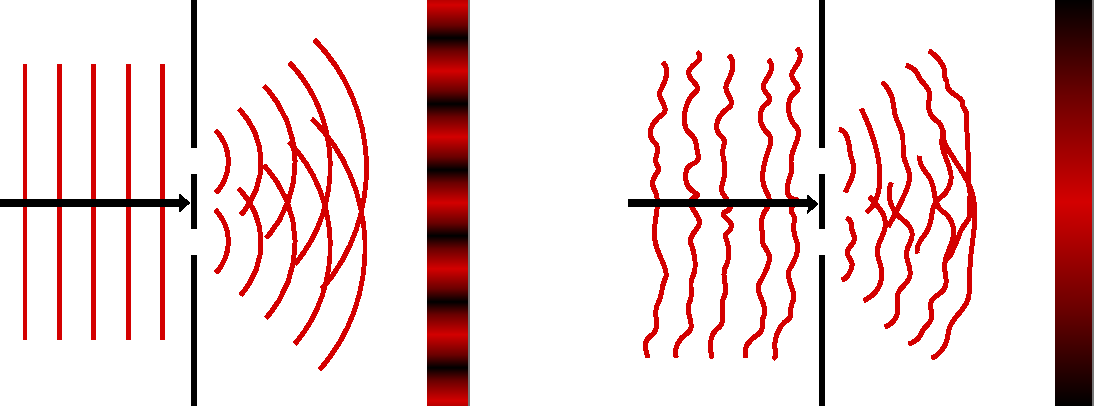
\includegraphics[width=10truecm]{slike/02_Young.pdf}
\caption{Youngov poskus na dveh režah. Le če je vpadno valovanje koherentno (levo), 
se pojavi na zaslonu interferenčni vzorec. Nekoherentno valovanje s spremenljivo
fazo (desno) ne da interferenčnega vzorca.}
\label{fig:Young}
\end{figure}

Svetloba navadnih svetil, na primer plinskih razelektritvenih cevi, 
je zaradi vrste nastanka kaotične narave. 
Atomi sevajo neodvisno, zato se faza izsevanega valovanja
spreminja. Približno konstantna je le znotraj nekega karakterističnega
časa. Če je pri interferenčnem poskusu karakteristični čas spreminjanja
faze krajši od zakasnitve med valovanjema, ki nastane zaradi različno
dolgih poti, pride na danem mestu zaslona do izmenično konstruktivne in 
destruktivne interference. Ker je čas spreminjanja praviloma
bistveno krajši od časa opazovanja interference,
utripanje svetlobe na zaslonu ni vidno. Interferenčni poskus se ne 
posreči zaradi majhne časovne koherence\index{Koherenca!časovna},
karakterističnemu času spreminjanja faze pa rečemo 
\index{Koherenčni čas}koherenčni čas
$t_{c}$. Časovno koherenco bomo natančneje obravnavali v razdelku
(\ref{sec:casovna-koherenca}), zaenkrat povejmo le, da je časovna
koherenca vezana na fazno razliko med dvema točkama, ki ležita
vzdolž smeri širjenja valovanja. 

Poleg časovne koherence na interferenčno sliko pomembno vpliva tudi
\index{Koherenca!prostorska}prostorska koherenca, ki je posledica
končne dimenzije svetila. Svetloba, ki na reži vpada iz različnih delov
svetila, ima namreč različno fazo zaradi razlike v dolžini poti od
svetila do rež. Ta faza se prišteje fazni razliki zaradi različno dolgih poti 
od rež do zaslona, zato se interferenčne proge na zaslonu nekoliko 
premaknejo. Če je fazna razlika žarkov iz različnih
delov svetila večja od fazne razlike za režami, se celotna interferenčna
slika na zaslonu izpovpreči. Interferenca se pri Youngovem poskusu
pojavi, kadar sta reži razmaknjeni le toliko, da je povprečna fazna
razlika manjša od $2\pi$. Največjemu prečnemu razmiku, ki še da interferenco,
rečemo prečna koherenčna razdalja\index{Koherenčna razdalja} $d_{c}$. 
Prostorska koherenca, ki jo bomo podrobneje spoznali v razdelku 
(\ref{Prostorska-koherenca}),
je torej vezana na fazno razliko med dvema točkama, ki ležita prečno 
na smer širjenja valovanja.

Poudarimo še enkrat, da je pojem koherence statističen.
Če je koherenčni čas $t_{c}$ dolg v primerjavi s časom opazovanja,
se seštevajo amplitude valovanj in pojavi se interferenčna slika.
Ta se slučajno spreminja z značilnim časom $t_{c}$. Če pa so razlike
poti večje od $ct_{c}$ ali razmik rež večji od $d_{c}$, gledamo
le povprečno sliko in interferenčne proge izginejo.

\section{Koherenca navadnih svetil}
\label{chap:kns}
Obravnavajmo plinsko razelektritveno cev in z
ustreznim filtrom izberimo eno samo spektralno črto. Ta črta naj ima
osrednjo frekvenco $\nu_{0}$ in končno frekvenčno širino $\Delta\nu$,
ki je kombinacija naravne širine, razširitve zaradi trkov med atomi in 
Dopplerjevega pojava (glej poglavje~\ref{Razsiritev}). Privzemimo,
da je glavni prispevek k razširitvi spektralne črte zaradi med\-atomskih
trkov, razširitev, povezano z Dopplerjevim pojavom, pa zanemarimo.

Celotna izsevana svetloba je vsota delnih valov, ki izhajajo iz posameznih
atomov in so med seboj neodvisni. Vsak delni val ohranja med trkoma,
to je v intervalu $t_{c}$, konstantno fazo. Valovni paket dolžine 
$t_{c}$ mora tako vsebovati frekvence v pasu $\Delta \nu$,
za katerega velja $t_{c}\Delta\nu\sim1$. Koherenčni čas je torej
kar reda velikosti obratne vrednosti spektralne širine svetlobe. Povsem
monokromatsko valovanje bil imelo neskončen koherenčni čas in bi bilo
popolno koherentno.

Zapišimo še izsevano polje takega svetila. 
Jakost električnega polja v izbrani točki prostora je vsota delnih
valov, ki izvirajo iz raznih delov izvora. Vsak atom v izvoru, naj
jih bo $N$, seva neodvisno, zato so tudi delna valovanja med seboj
neodvisna. Posamična valovanja ohranjajo konstantno fazo v času med
dvema trkoma atoma $t_{c}$. Zaradi enostavnosti privzemimo,
da so amplitude $E_{1}$ in polarizacije izsevanih polj posameznih atomov enake. 
Električno poljsko jakost $E$ v izbrani točki prostora potem 
zapišemo kot vsoto posameznih prispevkov
\begin{equation}
E=E_{1}\sum_{n=1}^{N}e^{i\phi_{n}(t)}.
\label{eq:amplituda-random}
\end{equation}
kjer se faza polja $\phi_{n}(t)$, ki ga izseva posamezni atom, naključno
spremeni ob trku z drugim atomom. Povprečje vsote polj je nič, 
povprečni kvadrat skupnega polja, ki je sorazmeren
z gostoto svetlobnega toka, pa je $NE_{1}^{2}$. Zaradi slučajnosti faz je 
slučajna tudi faza celotnega polja in se gotovo povsem spremeni v času, ko se
spremeni faza posameznih prispevkov, to je $t_{c}$. S tako svetlobo bomo videli 
interferenco na režah, če bo razlika poti delnih valovanj manjša od $c\, t_{c}$.

Oglejmo si izračun
na primeru. Imejmo $N=100$ neodvisnih atomov, ki se jim faza naključno
spreminja s karakterističnim časom $t_{c}=10/\nu$, kjer je $\nu$
frekvenca valovanja. Na sliki (\ref{fig:amplituda-intenziteta}) sta
prikazana časovna poteka amplitude $E$ (enačba \ref{eq:amplituda-random})
in $|E|^{2}$, ki je sorazmeren z intenziteto svetlobe.
\begin{figure}
\centering
\def\svgwidth{150truemm} 
\input{slike/02_fluktuacije02.pdf_tex}\\
\def\svgwidth{150truemm} 
\input{slike/02_fluktuacije01.pdf_tex}\\
\def\svgwidth{150truemm} 
\input{slike/02_fluktuacije03.pdf_tex}\\
\def\svgwidth{150truemm} 
\input{slike/02_fluktuacije04.pdf_tex}\\
\caption{Zgoraj: shematski prikaz električne poljske jakosti 
ravnega vala s konstantno fazo (rdeča črta) in električne
poljske jakosti navadnega svetila (modra črta) kot funkcije
časa. Faza polja se naključno spreminja s karakterističnim časom $t_{c}$.
Spodaj: intenziteta ravnega vala (rdeča črta) in intenziteta
svetlobe navadnega svetila (modra črta) kot funkciji
časa. Modra črtkana črta je povprečna intenziteta 
$\frac{1}{T}\int_{-T/2}^{T/2}E(t+t')E^{*}(t+t')dt'$
s časom integracije $T=t_{c}$. }
\label{fig:amplituda-intenziteta}
\end{figure}
Za primerjavo je prikazan tudi ravni val\index{Ravni val} $E=\sqrt{N}E_{1}e^{-i\omega t}$
s konstantno fazo in njegova intenziteta. Intenziteta ravnega vala je konstantna, 
medtem ko je povprečna intenziteta svetlobe navadnega svetila približno 
konstantna le znotraj $t_{c}$.

\section{Časovna koherenca}
\label{sec:casovna-koherenca}

Časovno koherenco\index{Koherenca!časovna} je najpreprosteje obravnavati 
z \index{Michelsonov interferometer}Michelsonovim 
interferometrom\footnote{Ameriški fizik in nobelovec Albert Abraham Michelson, 1852--1931.},
ki je prikazan na sliki (\ref{fig:michelson}). 
\begin{figure}[!h]
\centering
\def\svgwidth{85truemm} 
\input{slike/02_Michelson.pdf_tex}\\
\caption{\label{fig:michelson}Michelsonov interferometer. Svetlobo
iz izvora $P$ usmerimo preko kolimacijske leče (L) na polprepustno
zrcalo (PZ), s čimer jo razdelimo na dva snopa. S premikanjem 
enega zrcala (Z) spreminjamo zakasnitev enega delnega žarka. Interferenco opazujemo na detektorju.}
\end{figure}

Valovanje iz točke $P$ na polprepustnem 
zrcalu razdelimo na dva delna snopa, nato enega s premikanjem zrcala zakasnimo za $\tau=2x/c$.
S kolimacijsko lečo dosežemo, da je čim več žarkov, ki izhajajo iz
$P$, vzporednih z osjo interferometra. Dokler je zakasnitev
$\tau$ manjša od koherenčnega časa $t_{c}$, bosta snopa med seboj interferirala.
S spreminjanjem lege zrcala se tako na detektorju izmenično pojavijo ojačitve in oslabitve.
V primeru, da snop svetlobe ni povsem vzporeden, se na detektorju pojavijo 
osvetlitve v obliki interferenčnih krogov. Pri zakasnitvah,
ki so večje od koherenčnega časa, ni stalne fazne povezave, interferenčna
slika se spreminja in v daljših časih izpovpreči. Zapišimo to ugotovitev
še matematično.

Svetlobni tok na detektorju je sorazmeren s kvadratom električne
poljske jakosti obeh delnih valovanj
\begin{equation}
|E_{d}(t)|^{2}=|E(t)+E(t+\tau)|^{2}=|E(t)|^{2}+|E(t+\tau)|^{2}+2\Re E(t)E^{*}(t+\tau).
\label{eq:Michelson-intenziteta}
\end{equation}
Zakasnitev $\tau$ je določena s premikom pomičnega zrcala $\tau=2x/c$.
Navadno opazujemo v času $T$, ki je dolg v primerjavi s koherenčnim
časom, zato svetlobni tok povprečimo po času
\begin{eqnarray}
\langle|E_{d}(t)|^{2}\rangle & = & \frac{1}{T}\int_{-T/2}^{T/2}|E{}_{d}(t)|^{2}\, dt\nonumber \\
 & = & 2\langle|E|^{2}\rangle+2\Re\langle E(0)E^{*}(\tau)\rangle = 2\langle|E|^{2}\rangle+2\Re G(\tau).
\end{eqnarray}
Prvi člen je vsota povprečnih svetlobnih tokov obeh delnih snopov. Privzeli
smo, da je polje v povprečju stacionarno in je zato povprečje neodvisno
od izbire časovnega intervala. Drugi člen opisuje interferenco\index{Interferenca}. 
Za opis smo vpeljali
časovno avtokorelacijsko funkcijo\index{Avtokorelacijska funkcija}
električnega polja 
\boxeq{eq:avtokorelacija}{
G(\tau)=\frac{1}{T}\int_{-T/2}^{T/2}E(t)E^{*}(t+\tau)\, dt.
}
Za majhne zakasnitve $\tau$ na
detektorju zaznamo interferenco. Pri zakasnitvah, ki so precej
večje od koherenčnega časa $t_{c}$, sta polji $E(0)$ in $E(\tau)$
statistično neodvisni in povprečje produkta je enako produktu povprečij.
Ker je $\langle E(t)\rangle=0$, pri velikih zakasnitvah $\tau$ interferenčni
člen izgine in svetlobni tok je enak vsoti tokov posameznih delnih
snopov. 

Priročno je vpeljati normirano avtokorelacijsko funkcijo 
\begin{equation}
g(\tau)=\frac{G(\tau)}{G(0)}.
\label{eq:avtokorelacija-norm}
\end{equation}
Za povsem koherentno valovanje je $|g(\tau)|=1$, za povsem nekoherentno
valovanje je $|g(\tau)|=0,$ za delno koherentna  pa $0<|g(\tau)|<1$.
Praviloma se vrednost $|g(\tau)|$ z naraščajočim $\tau$ zmanjšuje,
saj postaja valovanje za velike časovne zamike vedno manj korelirano.
Ohlapno povedano je koherenčni čas zakasnitev, pri kateri postane
vrednost avtokorelacijske funkcije majhna.
Koherenčni čas\index{Koherenčni čas} $t_{c}$ lahko tudi bolj natančno definiramo 
z normirano avtokorelacijsko funkcijo
\boxeq{eq:koherencni-cas}{
t_{c}=\int_{-\infty}^{\infty}\left|g(\tau)\right|^{2}\, d\tau.
}
Zakasnitev delnih valov je pogosto posledica
različno dolgih optičnih poti, zato namesto koherenčnega časa 
uporabljamo tudi koherenčno dolžino\index{Koherenčna dolžina} $l_{c}=ct_{c}$. 
Pri tem moramo paziti, da koherenčne dolžine, ki jo izpeljemo iz časovne 
koherence, ne zamenjamo s prečno koherenčno
razdaljo, o kateri bomo govorili v nadaljevanju.

\begin{definition}
Pokaži, da v navedenih avtokorelacijskih
funkcijah $g(\tau)$ spremenljivka $t_{c}$ ustreza koherenčnemu času,
kot je definiran v enačbi (\ref{eq:koherencni-cas}), in izračunaj $|g(t_{c})|$ za oba primera.
\begin{equation}
g(\tau)=\begin{cases}
\exp\big(i\omega_{0}\tau-\left|\tau\right|/t_{c}\big),\\
\exp\big(i\omega_{0}\tau-\pi\tau^{2}/2t_{c}^{2}\big),
\end{cases}
\label{eq:gauss-eksponent}
\end{equation}

Ob nalogi (\ref{naloga-spekter}) in v razdelku~(\ref{Razsiritev}) 
bomo spoznali, da sta to avtokorelacijski
funkciji za svetlobo z \index{Spekter!Lorentzov}Lorentzovim spektrom
(razširitev spektralne črte zaradi trkov) in Gaussovim spektrom\index{Spekter!Gaussov}
(Dopplerjeva razširitev)\index{Dopplerjeva razširitev}.
\end{definition}

Poglejmo še nekaj značilnih koherenčnih dolžin. 
Koherenčna dolžina svetlobe, izsevane iz črnega telesa, je $l_{c}=ct_{c}\approx 
\hbar c/k_{B}T$ (glej nalogo~\ref{naloga-Planck})\index{Sevanje črnega telesa}. 
Svetloba s Sonca ($T \approx 6000$~K)
ima tako koherenčno dolžino zgolj $\sim 0,4~\si{\micro\metre}$. Svetloba,
izsevana iz LED sijalk\index{LED}, ima koherenčno dolžino $\sim20$--$100~\si{\micro\metre}$.
Če želimo povečati koherenčno dolžino taki svetlobi, jo moramo usmeriti
na ustrezne filtre in ji s tem zmanjšati spektralno območje.
Ožje spektralno območje ima na primer živosrebrna svetilka, zato je koherenčna
dolžina svetlobe za izbrano spektralno črto do okoli $50~\si{\centi\metre}$.
Koherenčna dolžina laserjev z ozko spektralno črto je tipično okoli
$100~\si{\metre}$, v nekaterih vlakenskih laserjih\index{Laser!vlakenski} 
pa koherenčna dolžina presega $100~\si{\kilo\metre}$.

\section{Zveza med avtokorelacijsko funkcijo in spektrom}

Spoznali smo, da je monokromatski ravni val povsem koherenten in njegov
korelacijski čas neskončen. Obravnavajmo zdaj koherenco poljubnega valovanja, ki
je v povprečju stacionarno. To pomeni, da se v času meritve povprečna intenziteta
ne spreminja. Vzamemo vzorec valovanja, ki traja čas $T$, in ga razvijemo 
v Fourierevo vrsto
\begin{equation}
E(t)=\sum_{n}A_{n}(\omega)e^{-in\Delta\omega t},\mbox{\hskip1cm}\Delta\omega=\frac{2\pi}{T}.
\end{equation}
Amplitude $A_{n}(\omega)$ so slučajne spremenljivke, ki predstavljajo delež polja pri 
krožni frekvenci $\omega=n\Delta\omega$, 
čas $T$ pa označuje čas opazovanja in mora biti bistveno daljši od $t_{c}$. 
Zapišimo amplitude $A_n$
\begin{equation}
A_{n}(\omega)=\frac{1}{T}\int_{-T/2}^{T/2}E(t)\, e^{i\omega t}\, dt.\label{eq:amplituda-An}
\end{equation}
 Vemo, da je kvadrat $|A_{n}(\omega)|^{2}$ sorazmeren gostoti 
svetlobnega toka pri krožni frekvenci $\omega$. Potem lahko vpeljemo 
\index{Spekter}spekter $S(\omega)$, ki podaja intenziteto svetlobe pri $\omega$,
deljeno z intervalom $\Delta\omega$\footnote{Gostota 
svetlobnega toka\index{Gostota energijskega toka} 
je $j = \varepsilon \varepsilon_0 c |E|^2/2$
z enotami W/m$^2$. Zaradi poenostavitve bomo namesto $j$ pogosto pisali intenziteto 
$I = |E|^2$, konstantne člene pa dodali le, če bomo rabili točno numerično vrednost.} 
\begin{equation}
S(\omega)=\frac{|A_{n}(\omega)|^{2}}{\Delta\omega}=\frac{T}{2\pi}|A_{n}(\omega)|^{2}.
\end{equation}
Vstavimo še amplitudo $A_{n}$ (enačba \ref{eq:amplituda-An}) in dobimo 
\begin{equation}
S(\omega) =\frac{1}{2\pi T}\int\int_{-T/2}^{T/2}E(t)E^{*}(t^{\prime})\, 
e^{-i\omega(t^{\prime}-t)}\, dt\, dt^{\prime}.
\end{equation}
Uvedemo novo spremenljivko $\tau=t^{\prime}-t$ in zapišemo
\begin{equation}
S(\omega)=\frac{1}{2\pi T}\int_{-\infty}^{\infty}e^{-i\omega\tau}d\tau\int_{-T/2}^{T/2}E(t)E^{*}(t+\tau)\, dt.
\label{eq:spekter}
\end{equation}
Opazimo, da je integral po $t$ ravno enak korelacijski funkciji $G(\tau)$. Ker je $T\gg t_{c}$,
je korelacijska funkcija na mejah integracije po enaka $\tau$ nič, zato
smo meje integracije po $\tau$ lahko raztegnili do neskončnosti. Zveza, ki smo jo dobili, je 
\index{Wiener-Hinčinov izrek} 
Wiener-Hinčinov izrek\footnote{Ameriški matematik Norbert Wiener, 1894--1964, in 
ruski matematik Aleksander Jakovljevič Hinčin, 1894--1959.}
\boxeq{eq:spekter-zveza}{
S(\omega)=\frac{1}{2\pi}\int_{-\infty}^{\infty}G(\tau)e^{-i\omega\tau}\, d\tau\;\Longleftrightarrow\; G(\tau)=\int_{-\infty}^{\infty}S(\omega)e^{i\omega\tau}\, 
d\omega.
}
Spekter svetlobe je torej Fouriereva transformiranka avtokorelacijske
funkcije svetlobnega polja. Pri tem ne pozabimo, da je spekter, ki smo ga zapisali z enačbo~(\ref{eq:spekter}), zapisan za izbran vzorec valovanja, 
ki traja čas $T$, in je tudi slučajna spremenljivka. Povprečen spekter dobimo tako, da naredimo
limito $T \rightarrow \infty$. 
\begin{equation}
\langle S (\omega) \rangle = \lim_{T\to \infty}S(\omega).
\end{equation}
\vglue-1truecm
\begin{remark}
Zaradi priročnosti smo zapisali spekter in Wiener-Hinčinov izrek s krožno frekvenco. Podobno lahko vpeljemo tudi spekter na frekvenčni interval in Wiener-Hinčinov izrek se prepiše v
\beq
S(\nu)=\int_{-\infty}^{\infty}G(\tau)e^{-i\,2 \pi \nu\tau}\, d\tau\;\Longleftrightarrow\; G(\tau)=\int_{-\infty}^{\infty}S(\nu)e^{i\,2\pi\nu \tau}\, d\nu.
\eeq
\end{remark}
Iz Wiener-Hinčinovega izreka (enačba~\ref{eq:spekter-zveza}) neposredno sledi, da je 
koherenca povezana s spektrom. Koherenčni čas $t_{c}$ je tako povezan s spektralno 
širino svetlobe $\gamma$, za katero velja (glej nalogo~\ref{naloga:gammatc})\index{Koherenčni čas}
\boxeq{eq:spektralna-sirina-zveza}{
\gamma=\frac{1}{t_{c}}.
}
\begin{definition}
\label{naloga:gammatc}
Formalno lahko vpeljemo spektralno širino kot 
\begin{equation}
\gamma=\frac{1}{2\pi\int_{-\infty}^{\infty}\left|s(\omega)\right|^{2}\, d\omega}; \quad
\mathrm{kjer~je} \quad
s(\omega)=\frac{S(\omega)}{\int_{-\infty}^{\infty}S(\omega) d\omega} =\frac{S(\omega)}{G(0)}
\label{eq:spektralna-sirina}
\end{equation}
normirani spekter. 
Z uporabo enačbe za koherenčni čas $t_{c}$ (enačba \ref{eq:koherencni-cas})
pokaži, da je spektralna širina obratno sorazmerna s koherenčnim
časom (enačba \ref{eq:spektralna-sirina-zveza}) ne glede na
obliko spektra. Namig: Uporabi Parsevalov izrek, ki pravi:
\begin{equation}
\int_{-\infty}^{\infty}\left|f(t)\right|^{2}\, dt={2\pi}
\int_{-\infty}^{\infty}\left|F(\omega)\right|^{2}\, d\omega,
\end{equation}
kjer je 
\beq
F(\omega)=\frac{1}{2\pi} \int_{-\infty}^{\infty}f(t)e^{-i\omega\tau}\, d\tau
\eeq
Fouriereva transformiranka funkcije $f(t)$.
\end{definition}

Za zgled Wiener-Hinčinovega izreka vzemimo primer, ki je predstavljen na 
sliki~(\ref{fig:amplituda-intenziteta}). 
Ker so trki med atomi naključni, je avtokorelacijska funkcija eksponentno pojemajoča
\beq
g(\tau)=e^{i\omega_{0}\tau} e^{-\tau/t_{c}},
\label{eq:g-primer}
\eeq
spekter take svetlobe pa je Lorentzove oblike\index{Spekter!Lorentzov} (glej nalogo~\ref{naloga-spekter})
\begin{equation}
s(\omega)=\frac{1}{\pi}\frac{\gamma}{(\omega-\omega_{0})^{2}+\gamma^{2}},
\label{eq:spekter-primer}
\end{equation}
pri čemer je $\gamma=1/t_{c}$ spektralna širina. 
Normirani spekter $s(\omega)$ in ustrezna avtokorelacijska funkcija $g(\tau)$ 
sta prikazana na sliki~(\ref{fig:SpekterAc}). 
Točke na grafih 
predstavljajo spekter in izračunano avtokorelacijsko funkcijo 
za integracijski čas $T=100\,t_{c}$. Za primerjavo sta z rdečo 
krivuljo prikazana tudi pričakovan spekter (enačba~\ref{eq:spekter-primer}) in avtokorelacijska
funkcija (enačba~\ref{eq:g-primer}). Zaradi končnega
časa $T$ pri izračunu povprečja se spekter iz simulacije nekoliko razlikuje
od pričakovane vrednosti. 
\begin{figure}[h]
\centering
\def\svgwidth{65truemm} 
\input{slike/02_spekter.pdf_tex}\qquad
\def\svgwidth{65truemm} 
\input{slike/02_avtokorelacija.pdf_tex}
\caption{Spekter in avtokorelacijska funkcija valovanja s slike~(\ref{fig:amplituda-intenziteta})}
\label{fig:SpekterAc}
\end{figure}

\begin{definition}
\label{naloga-spekter}
Imejmo dve vrsti svetlobe. Prva naj ima avtokorelacijsko funkcijo, ki je eksponentno pojemajoča, druga
pa ima avtokorelacijsko funkcijo Gaussove oblike (enačbi~\ref{eq:gauss-eksponent}). Pokaži, da sta njuna
spektra oblike\index{Spekter!Gaussov}\index{Spekter!Lorentzov}
\begin{equation}
s(\omega)=
\frac{1}{\pi}\frac{\gamma}{(\omega-\omega_{0})^{2}+\gamma^{2}} \quad \mathrm{in} \quad 
s(\omega)= \frac{1}{\sqrt{2}\pi\gamma}\exp\big(-
\frac{\left(\omega-\omega_{0}\right)^{2}}{2\pi\gamma^{2}}\big),
\end{equation}
kjer je $\gamma=1/t_{c}$ spektralna širina. 
\end{definition}

Spektralne črte atomov so pogosto Lorentzove oblike, kar je posledica
eksponentnega razpada stanj (naravna širina). Dodatno se spektralne
črte razširijo zaradi trkov med atomi, vendar tudi to vodi do približno Lorentzove
oblike spektra. V plinih je pogosto prevladujoča razširitev črt
zaradi Dopplerjevega pojava (glej razdelek~\ref{Razsiritev}). 
Spekter Dopplerjevo razširjene svetlobe je, kot bomo videli v 
nadaljevanju, Gaussove oblike. V tem primeru iz enačbe~(\ref{eq:spekter-zveza})
sledi, da je tudi avtokorelacijska funkcija Gaussove oblike.
\vglue1truecm

\begin{definition}\label{naloga-Planck}
Numerično pokaži, da je koherenčni čas svetlobe, ki jo oddaja črno telo s 
temperaturo $T$, približno enak $t_{c}\approx{\hbar}/{k_{B}T}$.\index{Sevanje črnega telesa}
Normirani spekter sevanja črnega telesa zapišemo 
kot \index{Spekter!Planckov}Planckov spekter 
\begin{equation}
s(\omega)=\frac{15}{\pi^{4}} \frac{\hbar^4\omega^3}{(kT)^4}/\left(e^{\hbar\omega/kT}-1\right)
\quad \textrm{za}~\omega >0,~\textrm{sicer}~s(\omega) = 0.
\label{eq:Planckov-spekter}
\end{equation}
\end{definition}

\begin{remark}\index{Fouriereva spektroskopija}
V prejšnjem razdelku smo videli, da časovno avtokorelacijsko funkcijo
merimo z Michelsonovim interferometrom. Dobljena povezava med merjeno
avtokorelacijo in izračunanim spektrom je osnova za Fourierevo 
spektroskopijo\footnote{Francoski matematik in fizik Jean Baptiste Joseph Fourier, 1768--1830.},
ki ima nekatere pomembne prednosti pred drugimi metodami in se danes
precej uporablja, posebej v infrardečem delu EM valovanja.\index{Infrardeče valovanje}
\end{remark}

\section{Prostorska koherenca}
\label{Prostorska-koherenca}
\index{Koherenca!prostorska}
Vrnimo se k Youngovemu poskusu\index{Youngov poskus} in obravnavi interference
\index{Interferenca} na dveh ozkih režah. 
Osvetljujmo zdaj reži s svetilom končnih razsežnosti. Svetilo naj sveti skoraj enobarvno
svetlobo in naj bo na simetrali med režama, kot kaže slika~(\ref{fig:shema-interferenca}).

Žarka, ki izhajata iz sredine svetila (polna črta), 
opravita do rež v ravnini A enako dolgo pot in povzročita na zaslonu B 
interferenčne proge. Žarka, ki izhajata iz roba izvora (prekinjena črta), 
imata do rež različno dolgo pot, zato nastane med njima fazna razlika že do ravnine A, 
ki se prišteje fazni razliki do ravnine B. Interferenčne proge, ki jih tvorita 
robna žarka, so premaknjene glede na proge centralnih žarkov. Ker so žarki z roba
statistično neodvisni od žarkov iz sredine, z njimi
ne interferirajo. Celotni interferenčni vzorec je zato kar vsota interferenčnih
vzorcev žarkov iz različnih delov svetila. Če je razlika poti za žarke
iz različnih delov velikosti valovne dolžine $\lambda$, se celotna
interferenčna slika na zaslonu B izpovpreči.

\begin{figure}[h]
\centering
\def\svgwidth{140truemm} 
\input{slike/02_precnaKoherenca.pdf_tex}
\caption{Shema interferenčnega eksperimenta z razsežnim svetilom}
\label{fig:shema-interferenca}
\end{figure}

Razdaljo med režama $d_c$, pri kateri interferenčne proge
izginejo, imenujemo\index{Koherenčna razdalja} prečna koherenčna razdalja. 
Zanjo velja približno 
\begin{equation}
\delta s = d_c\sin\varphi\approx d_c\frac{R}{z}\sim\lambda\;\Rightarrow\;
d_{c}\sim\frac{z\lambda}{R}.
\label{eq:prost_koh}
\end{equation}
Pogosto je v uporabi
tudi pojem \index{Koherenčna ploskev}koherenčna ploskev, to je območje, 
v katerem je fazna razlika v povprečju konstantna. Velikost te ploskve je približno $d_{c}^{2}$.
V območju koherenčne ploskve so tudi valovne fronte približno gladke.

Zapišimo gornje ugotovitve nekoliko bolj natančno. Na zaslonu $B$
izmerimo gostoto svetlobnega toka, ki je sorazmerna povprečju kvadrata
električne poljske jakosti valovanj, ki izhajata iz obeh odprtin
\begin{align}
\langle|E{}_{d}|^{2}\rangle & =\langle|K_{1}E_{1}+K_{2}E_{2}|^{2}\rangle\nonumber \\
&=  |K_{1}|^{2}\langle|E_{1}|^{2}\rangle+|K_{2}|^{2}\langle|E_{2}|^{2}\rangle+
2\Re K_{1}K_{2}^{*}\langle E_{1}(0)E_{2}^{*}(\tau)\rangle.
\end{align}
Pri tem je je $\tau=d\sin\vartheta/c$ zakasnitev valovanja iz druge odprtine
glede na valovanje iz prve, faktorja $K_{1}$ in $K_{2}$ pa sta določena
z uklonom na posameznih odprtinah.
Interferenčna slika je vsebovana v podobnem členu kot pri Michelsonovem
interferometru, le da nastopa v tem primeru namesto avtokorelacijske funkcije
navzkrižna korelacijska funkcija polj $E_{1}$ in $E_{2}$ iz obeh
odprtin.\index{Navzkrižna korelacijska funkcija} 

Kako je interferenčni člen povezan z lastnostmi svetila, brez težav
doženemo v izbranem primeru skoraj enobarvne svetlobe z osrednjo krožno frekvenco
$\omega$. Tedaj lahko za zakasnitve $\tau$, ki so krajše
od koherenčnega časa, zapišemo 
\begin{equation}
E_{2}(\tau)=E_{2}(0)\, e^{-i\omega\tau}
\end{equation}
 in 
\begin{equation}
\langle E_{1}(0)E_{2}^{*}(\tau)\rangle=\langle E_{1}(0)E_{2}^{*}(0)\rangle 
e^{i\omega\tau}=J(P_{1},P_{2})\, e^{i\omega\tau}.
\end{equation}
Faktor $\Re e^{i\omega\tau}= \cos(\omega \tau) = \cos(kd\sin\vartheta)$ da interferenčne
proge za koherentno osvetlitev zaslona, povprečje produkta polj
v odprtinah ob istem času $J(P_{1},P_{2})=\langle E(P_{1},0)E^{*}(P_{2},0)\rangle$
pa meri stopnjo prečne koherence med obema odprtinama. Od velikosti
tega člena je odvisen kontrast interferenčnih prog. Izračunajmo ga.

Polje v posamezni odprtini je vsota prispevkov iz celega izvora.
\begin{equation}
E(P_{j})=-\frac{i}{\lambda}\int E(\xi,\eta)\frac{e^{iks_{j}}}{s_{j}}\, d\xi\, d\eta.
\end{equation}
Pri tem je $s_{j}$ razdalja med točko $(\xi,\eta)$ na izvoru in točko
$P_{j}(x_{j},y_{j})$ na reži v ravnini A (glej sliko \ref{fig:shema-interferenca}).
Faktor pred integralom $-i/\lambda$ izhaja iz uklonske teorije (enačba~\ref{eq:Fresnel-Kirchoffov-integral}).
Tako je 
\begin{equation}
J(P_{1},P_{2})=\frac{1}{\lambda^{2}}\int\int\langle E(\xi,\eta)E^{*}(\xi^{\prime},\eta^{\prime})\rangle\frac{e^{ik(s_{1}-s_{2}^{\prime})}}{s_{1}s_{2}^{\prime}}\, d\xi\, d\eta\, d\xi^{\prime}d\eta^{\prime}.\label{eq:field-correlation}
\end{equation}
V izbranem svetilu sevajo atomi neodvisno. Valovanji iz dveh točk svetila,
ki sta razmaknjeni za več kot $\lambda$, sta neodvisni in povprečje
njunega produkta je enako nič. Tako približno velja 
\begin{equation}
\langle E(\xi,\eta)E^{*}(\xi^{\prime},\eta^{\prime})\rangle=\frac{\lambda^{2}}{\pi} \cdot \delta(\xi-\xi^{\prime},\eta-\eta^{\prime})\langle|E(\xi,\eta)|^{2}\rangle.
\label{eq:delta-Zernike}
\end{equation}
Faktor $\lambda^{2}/\pi$ poskrbi za ustrezno normalizacijo. 
Naj bo oddaljenost svetila od zaslona $A$
veliko večja od dimenzije svetila ($z\gg R$), tako da lahko imenovalec pod integralom
v izrazu~(\ref{eq:field-correlation}) nadomestimo z $z^{2}$ in postavimo
pred integral. Sledi
\begin{equation}
J(P_{1},P_{2})=\frac{1}{\pi z^{2}}\int\langle|E(\xi,\eta)|^{2}\rangle e^{ik(s_{1}-s_{2})}\, d\xi\, d\eta.\label{eq:Zernike1}
\end{equation}
Izraz lahko še nekoliko poenostavimo, če razvijemo $s_{1}$
in $s_{2}$ do drugega reda
\begin{equation}
s_{j}=\sqrt{z^{2}+(x_{j}-\xi)^{2}+(y_{j}-\eta)^{2}}\approx z+\frac{(x_{j}-\xi)^{2}+(y_{j}-\eta)^{2}}{2z}.
\end{equation}
Pri tem sta $(x_{j},y_{j})$ koordinati točke $P_{j}$. Pišimo 
še $\langle|E(\xi,\eta)|^{2}\rangle=I(\xi,\eta)$, ki je do konstante natančno
enak intenziteti valovanja, ter $x_{2}-x_{1}=\Delta x$
in $y_{2}-y_{1}=\Delta y$. S tem dobimo znani rezultat, tako imenovani \index{van Cittert-Zernikov izrek}
van Cittert-Zernikov izrek\footnote{Nizozemski fizik Pieter Hendrik van Cittert, 1889--1959, in 
nizozemski fizik in nobelovec Frits Zernike, 1888--1966.}
\boxeq{eq:Zernike2}{
J(\Delta x,\Delta y)=\frac{e^{-i\phi}}{\pi z^{2}}\int I(\xi,\eta)e^{ik(\Delta 
x\xi+\Delta y\eta)/z}\, d\xi\, d\eta.
}

Faza 
\begin{equation}
\phi=\frac{\pi}{\lambda z}[(x_{2}^{2}+y_{2}^{2})-(x_{1}^{2}+y_{1}^{2})]
\end{equation}
meri skupni premik interferenčnih prog, do katerega pride, kadar svetilo
ne leži na isti osi kot odprtini v zaslonu. Kadar ležita odprtini v ravnini $A$ 
simetrično glede na os svetila, je faza $\phi$ enaka nič.

Dobljeni rezultat si je vredno nekoliko ogledati. Prečno prostorsko
korelacijsko funkcijo $J(P_{1},P_{2})$, ki določa kontrast interferenčnih
prog, smo izrazili kot 2-D  Fourierevo transformiranko intenzitete svetlobe
na samem svetilu (enačba \ref{eq:Zernike2}). 
\begin{remark}
Ob tem se spomnimo,
da velja podobna zveza med električno poljsko jakostjo v osvetljeni odprtini 
in njeno Fraunhoferjevo uklonsko sliko (enačba~\ref{eq:FraunhoferApprox}), 
pri čemer so količine, ki nastopajo v obeh zvezah,
povsem različne. Različna je tudi veljavnost obeh izrazov: medtem ko je Fraunhoferjeva
uklonska formula veljavna le v veliki oddaljenosti, za opis uklonske slike v bližnjem polju
pa je treba uporabiti Fresnelov izraz (enačba~\ref{eq:FresnelApprox}), 
je rezultat za $J(P_{1},P_{2})$ (enačba~\ref{eq:Zernike2}) veljaven v obeh območjih.\index{Fraunhoferjev uklon}
\index{Fresnelov uklon}
\end{remark}

Ker je velikost svetila končna, $J(P_{1},P_{2})$ pri dovolj veliki
razdalji med točkama $P_{1}$ in $P_{2}$ gotovo pade na nič. Največja
razdalja, do katere je $J(P_{1},P_{2})$ še različna od nič, je ravno
prečna koherenčna razdalja $d_{c}$, ustrezna ploskev pa je koherenčna
ploskev $S_{c}$\index{Koherenčna ploskev}. Iz izraza za koherenčno razdaljo 
(enačba \ref{eq:prost_koh}) jo lahko ocenimo
\begin{equation}
S_{c}\sim\frac{(\lambda z)^{2}}{S_{0}}\sim\frac{\lambda^{2}}{\Omega_{0}},
\label{eq:koherencna-ploskev}
\end{equation}
kjer je $S_{0}$ površina svetila, $\Omega_{0}$ pa prostorski kot,
pod katerim je videti svetilo v ravnini $A$. 

Oglejmo si primer. Naj bo svetilo v obliki kroga 
s polmerom $R$, obe odprtini v zaslonu naj imata koordinati $y$  enaki nič, razmik
med režama v smeri $x$ pa naj bo $d$. 
Prečno korelacijsko funkcijo izračunamo iz enačbe~(\ref{eq:Zernike2}) in dobimo 
(glej nalogo~\ref{naloga:J})
\begin{equation}
J(0,\Delta y)=2\frac{R^{2}I_{0}}{z^{2}}\,\frac{J_{1}(kRd/z)}{kRd/z},
\label{eq:jkrozna}
\end{equation}
kjer je $J_{1}(x)$ Besslova funkcija. V ničlah Besslove funkcije
pade prečna korelacijska funkcija $J$ na nič in interferenčnega vzorca ne vidimo. 
Za prečno koherenčno razdaljo je zato smiselno vzeti ravno prvo ničlo Besslove funkcije
$J_1$, to je pri
\beq
\label{eq:okroglo_svetilo}
d_{c} \approx 3,83 \frac{z}{kR} = 0,61 \frac{\lambda z}{R}.
\eeq
\begin{definition}
\label{naloga:J}
Pokaži, da prečno korelacijsko funkcijo za okroglo svetilo s polmerom $R$, pri čemer
odprtini na zaslonu ležita simetrično na osi $y$ v razmiku $d$, zapišemo z enačbo~(\ref{eq:jkrozna}). 
\end{definition}

Doslej smo obravnavali le valovanje v središču interferenčne slike na
zaslonu $B$, to je pri tako majhnih kotih $\vartheta$, da je zakasnitev
manjša od koherenčnega časa. Pri večjih kotih moramo upoštevati še
vpliv končnega koherenčnega časa, zaradi česar se kontrast interferenčnih
prog še dodatno zmanjšuje. Interferenčna slika je 
tako produkt časovnega in prostorskega dela. 

V primeru dveh zelo tankih rež z razmikom $d$ nastanejo na zaslonu
$B$ uklonski vrhovi. Za nekaj različnih razmikov med odprtinama $d$ je intenziteta
svetlobe na zaslonu prikazana na sliki~(\ref{fig:Interferencna-slika}).
Če je $d\ll\lambda z/R$ (slika a), je modulacija interferenčnih prog v sredini
popolna in se zaradi končnega koherenčnega časa zmanjšuje le pri večjih
kotih $\vartheta$. Pri nekaj večjem razmiku (slika~b) tudi v sredini kontrast
ni več popoln. Obenem se interferenčne proge zgostijo. Kadar je $d\approx 3,83\,z/kR$,
dosežemo prvo ničlo Besslove funkcije $J_{1}(x)$ in interferenčni vzorec
prvič izgine (slika~c). Takrat je razdalja med režama ravno enaka prečni
koherenčni razdalji valovanja. Pri še večjih razmikih (slika~d) 
je Besslova funkcija negativna in ponovno se pojavijo interferenčne proge, 
vendar so slabše izražene in z nasprotno fazo, kar da v sredini temno progo. 
\index{Interferenca}

\begin{figure}[h]
\begin{center}
\def\svgwidth{0.37\textwidth} 
\input{slike/02_interferenca01.pdf_tex}
\def\svgwidth{0.37\textwidth} 
\input{slike/02_interferenca02.pdf_tex}
\def\svgwidth{0.37\textwidth} 
\input{slike/02_interferenca03.pdf_tex}
\def\svgwidth{0.37\textwidth} 
\input{slike/02_interferenca04.pdf_tex}
\caption{Interferenčna slika na zaslonu
$B$ za različne vrednosti razmikov med odprtinama: a) $d = z/kR$, b) $d=2z/kR$, 
c) $d = 3,832\,z/kR$ in d) $d = 5,136\,z/kR$. 
Z večanjem razdalje med režama se proge zgostijo in kontrast se zmanjša. Koherenčni
čas svetlobe je $t_{c}=10/\omega$, kar še dodatno zmanjšuje modulacijo
interferenčnih prog. Pri $d=3,832\,z/kR$ dosežemo prvo ničlo Besslove
funkcije in interferenčni vzorec popolnoma izgine. Nato se interferenčne
proge zopet pojavijo, vendar z manjšim kontrastom in nasprotno fazo.}
\label{fig:Interferencna-slika}
\end{center}
\end{figure}

\begin{remark}
Merjenje prečne koherenčne razdalje svetlobe
zvezd je osnova za Michelsonovo metodo določanja zvezdnih premerov.
Svetlobo izbrane zvezde zberejo v teleskop preko dveh manjših parov
zrcal, kjer sta zunanji zrcali na pomičnih rokah, tako da ju je mogoče
razmikati. Glavno zrcalo teleskopa zbere svetlobna snopa v goriščni
ravnini, kjer nastanejo interferenčne proge, če le pomični zrcali
nista preveč razmaknjeni. Iz razmika, pri katerem interferenčne proge
izginejo, je mogoče določiti premere bližnjih svetlih zvezd. Za zvezdo
s polmerom $10^{6}$ km v razdalji 5 svetlobnih let je prečna koherenčna
razdalja za zeleno svetlobo okoli $15$~m, kar je z Michelsonovim
zvezdnim interferometrom mogoče izmeriti. Pri zvezdah, ki so dlje
od nekaj deset svetlobnih let, metoda odpove.
\end{remark}


%Final

%-------------------------------------------------------------------------------
%	CHAPTER 3
%-------------------------------------------------------------------------------

\chapterimage{slike/Laguerre.jpg} % Chapter heading image

\chapter{Koherentni snopi svetlobe}
V tem poglavju bomo zapisali obosni približek valovne enačbe in spoznali 
njegovo osnovno rešitev, to je Gaussov snop. Obravnavali bomo tudi snope višjega reda in
se naučili računati prehode Gaussovih snopov skozi optične elemente. 

\section{Omejen snop svetlobe}
Pri obravnavi elektromagnetnega valovanja pogosto uporabljamo
približek ravnih valov. Ti so v smeri pravokotno na smer širjenja
neomejeni in so zato lahko le idealizacija. Čim raven val usmerimo skozi odprtino
v zaslonu, nastane omejen snop svetlobe. V snopu svetlobe valovna čela niso
ravna in meje snopa niso vzporedne, ampak se snop zaradi uklona širi\index{Uklon} 
(slika \ref{fig:Uklon-na-rezi}).
\begin{figure}[h]
\centering
\def\svgwidth{120truemm} 
\input{slike/03_uklon_na_rezi.pdf_tex}
\caption{Omejen snop nastane ob prehodu ravnega vala skozi končno odprtino.}
\label{fig:Uklon-na-rezi}
\end{figure}

V veliki oddaljenosti od zaslona polje izračunamo s
\index{Fraunhoferjev uklon}Fraunhoferjevo uklonsko teorijo (glej razdelek~\ref{FFuklon}). 
Vendar za oceno kota širjenja računa niti ne potrebujemo. Velja približno 
\begin{equation}
\vartheta\sim\frac{\lambda}{a},
\label{eq:kot_ocena}
\end{equation}
kjer je $a$ polmer odprtine v zaslonu.\index{Območje bližnjega polja}
Opis polja v bližini zaslona je zahtevnejši, saj je treba uporabiti 
Fresnelov približek\index{Fresnelov uklon} (enačba~\ref{eq:FresnelApprox}).
Območje bližnjega polja seže do $b$, ki ga ocenimo s slike (\ref{fig:Uklon-na-rezi})
\begin{equation}
\frac{a}{b}\sim{\vartheta}\sim \frac{\lambda}{a} \qquad \mathrm{in~tako} \qquad b\sim\frac{a^2}{\lambda}.
\label{eq:z_ocena}
\end{equation}

Bolj kvantitativen opis omejenih
snopov bi dobili s Fraunhoferjevo in Fresnelovo uklonsko teorijo,
kar ni najudobnejša pot (glej nalogo~\ref{ffuklon}). Lotimo se problema raje z 
uporabo obosnega približka valovne enačbe.

\begin{definition}
\label{ffuklon}
Pokaži, da je Fraunhoferjeva uklonska slika na odprtini, katere prepustnost se v radialni smeri
spreminja kot Gaussova funkcija $T(\xi, \eta)=e^{-(\xi^2+\eta^2)/w_0^2}$, podana z Gaussovo funkcijo
oblike $E(x,y,z) \propto e^{-(x^2+y^2)/w^2(z)}$ in določi odvisnost $w(z)$. Izračunaj še 
uklonsko sliko v bližnjem polju po Fresnelovi uklonski teoriji.
\end{definition}

\section{Obosna valovna enačba}
Obravnavo začnemo z valovno enačbo in monokromatskim valovanjem s krožno frekvenco $\omega$. Ustrezna
Helmholtzeva enačba je \index{Helmholtzeva enačba}(enačba~\ref{eq:Helmholtz})
\begin{equation}
\nabla^{2}E+k^{2}E=0,
\label{eq:valovna-enacba-hh}
\end{equation}
kjer je $k=n\omega/c_{0}$ valovno število in $n$ lomni količnik
sredstva, po katerem se valovanje širi. Zaradi enostavnosti obravnavamo
le eno polarizacijo, tako da $E$ pišemo kot skalar. Iščemo rešitev za
omejen snop, ki se širi približno vzdolž osi $z$. Uporabimo nastavek
\begin{equation}
E=E_{0}\psi(\mathbf{r},z)e^{ikz},
\label{eq:ravni-val-nastavek}
\end{equation}
kjer je $\mathbf{r}$ krajevni vektor v ravnini $xy$, prečni na smer širjenja svetlobe. 
Glavni del odvisnosti od koordinate $z$ smo zapisali v faktorju $e^{ikz}$, tako da lahko
privzamemo, da se $\psi$ v smeri $z$ le počasi spreminja. Vstavimo
gornji nastavek v Helmholtzevo enačbo (enačba~\ref{eq:valovna-enacba-hh})
in pri tem zanemarimo druge odvode $\psi$ po $z$, saj je zaradi počasnega spreminjanja
$\partial^{2}\psi/\partial z^{2}$ majhen v primerjavi s $k\partial\psi/\partial z$ in $k^{2}\psi$.
Dobimo obosno
ali paraksialno valovno enačbo\index{Obosna valovna enačba} za $\psi$
\index{Paraksialna enačba|see{Obosna valovna enačba}}
\boxeq{eq:obosna-valovna-enacba}{
\nabla_{\perp}^{2}\psi=-2ik{\frac{{\partial\psi}}{{\partial z}}}.
}
\begin{remark} 
Opazimo, da je obosna valovna enačba enaka Schr\"{o}dingerjevi enačbi\index{Schr\"odingerjeva enačba}
za prost delec v dveh dimenzijah, v kateri ima koordinata $z$ vlogo
časa. Omejenemu snopu v kvantni mehaniki ustreza lokaliziran delec
-- valovni paket. Ta se s časom širi, kar v optiki ustreza pojavu uklona.
\end{remark}
Preden se lotimo reševanja obosne valovne enačbe, jo primerjajmo s Helmholtzevo enačbo
na primeru ravnega vala. Nastavek za ravni val \index{Ravni val} zapišemo v obliki
\begin{equation}
\psi=e^{ik_{1}x+ik_{2}y}\, e^{-i\beta z}.
\label{eq:ravni-val-nastavek-obosni}
\end{equation}
Da bo gornji nastavek rešitev
obosne valovne enačbe~(enačba~\ref{eq:obosna-valovna-enacba}), mora veljati 
\begin{equation}
\beta=\frac{k_{1}^{2}+k_{2}^{2}}{2k}.
\end{equation}
Ko vstavimo nastavek za $\psi$ v izraz za polje $E$ 
(enačba~\ref{eq:ravni-val-nastavek}), dobimo ravni val, za katerega velja 
\begin{equation}
k_{3}=k-\beta=k-\frac{k_{1}^{2}+k_{2}^{2}}{2k}.
\label{eq:k3-razvoj}
\end{equation}
Pri tem $k_{3}$ označuje vzdolžno in $k_{1}$ ter $k_{2}$ prečni komponenti valovnega 
vektorja, $k$ pa je valovno število. Po drugi strani za ravni val, ki je 
rešitev Helmholtzeve enačbe (enačba~\ref{eq:valovna-enacba-hh}), velja zveza
\begin{equation}
k_{3}=\sqrt{k^{2}-(k_{1}^{2}+k_{2}^{2})}.\label{eq:k3-tocno}
\end{equation}
Vidimo, da sledi enačba~(\ref{eq:k3-razvoj}) iz enačbe~(\ref{eq:k3-tocno})
z razvojem za majhne vrednosti $k_1$ in $k_2$. To pove, da je približek obosne 
enačbe dober, kadar sta prečni komponenti valovnega vektorja 
majhni v primerjavi z vzdolžno. 
Takrat je majhen tudi kot širjenja snopa in člene, višje od kvadratnih,
lahko zanemarimo. To je tudi območje veljavnosti Fresnelove uklonske
teorije.\index{Fresnelov uklon}

\begin{remark}\index{Fouriereva optika}
Časovno odvisnost poljubnega začetnega
stanja v kvantni mehaniki navadno izračunamo tako, da v začetnem
trenutku paket razvijemo po lastnih stanjih energije -- ravnih valovih.
Rešitev v poljubnem kasnejšem trenutku je potem dana v obliki Fourierevega
integrala. Ta pot je zelo uporabna tudi v optiki in je osnova sklopa
računskih metod, znanih pod imenom Fouriereva optika. V našem primeru
z njo brez težav pridemo nazaj do Fresnelove uklonske formule.
\end{remark}

\section{Osnovni Gaussov snop}
\index{Gaussov snop}
Naša naloga je poiskati rešitve obosne valovne enačbe, ki popišejo omejene
snope. Iz kvantne mehanike vemo, da je najbolj lokaliziran in se najpočasneje
širi valovni paket Gaussove oblike. Zato poskusimo najti rešitev obosne
enačbe (enačba~\ref{eq:obosna-valovna-enacba}) z nastavkom
\begin{equation}
\psi(r,z)=e^{ikr^{2}/2q(z)}\, e^{-i\phi(z)},\label{eq:gaussov-snop-nastavek}
\end{equation}
kjer funkcija $q(z)$ opisuje širjenje snopa v prečni smeri,
$\phi(z)$ pa opisuje počasno spreminjanje faze snopa vzdolž osi $z$.
Vstavimo nastavek (enačba~\ref{eq:gaussov-snop-nastavek}) v obosno valovno enačbo 
(enačba~\ref{eq:obosna-valovna-enacba}). Zaenkrat se omejimo le na radialno 
simetrične rešitve in v cilindričnih koordinatah zapišemo
\begin{equation}
\nabla_{\perp}^{2}\psi=\frac{1}{r}\frac{\partial}{\partial r}\, r\,\frac{\partial\psi}{\partial r}=
\left( \frac{2ik}{q}-\frac{k^2r^2}{q^2}\right)\psi
\end{equation}
 in 
\begin{equation}
\frac{\partial\psi}{\partial z}=\left(-\frac{ikr^{2}}{2q^2}q(z)^{\prime}-i\phi^{\prime}\right)\psi.
\end{equation}
Iz obosnega približka sledi
\begin{equation}
\frac{2ik}{q}-\frac{k^2r^2}{q^2}=ik\left(\frac{ikr^{2}}{q^2}q(z)^{\prime}+2i\phi^{\prime}\right).
\end{equation}
Gornja zveza mora veljati pri vsakem $r$, zato sta koeficienta
pri $r^{2}$ na obeh straneh enačbe enaka in člena brez odvisnosti od $r$ prav tako. Sledi
\begin{equation}
q(z)^{\prime}=1\mbox{\hskip1cm in \hskip1cm}\phi^{\prime}=-\frac{i}{q}.
\end{equation}
Z integracijo dobimo najprej 
\begin{equation}
q=z-iz_{0},
\label{eq:alpha}
\end{equation}
kjer smo z $-i z_{0}$ označili integracijsko konstanto. 
Integriramo še enačbo za fazo 
\begin{equation}
\phi=\int_{0}^{z}\,-\frac{i dz}{z-iz_{0}}=-i\ln(1+i\frac{z}{z_{0}}).
\end{equation}
Sledi
\begin{equation}
\psi = \exp\left(i\frac{kr^{2}}{2(z-iz_0)}\right)\,\exp\left(-\ln(1+i\frac{z}{z_{0}})\right)
\end{equation}
in
\begin{equation}
 \psi = \frac{1}{1+i\frac{z}{z_{0}}}\,\exp\left(-\frac{kr^{2}z_{0}}{2(z_{0}^{2}+z^{2})}+
 \frac{ikr^{2}z}{2(z_{0}^{2}+z^{2})}\right).
 \label{eq:gaussov-snop-vmesni}
\end{equation}
Najprej poglejmo realni del eksponenta, ki opisuje prečno obliko snopa. Vpeljemo novo spremenljivko $w$
in realni del prečne odvisnosti zapišemo z Gaussovo funkcijo $\exp(-r^2/w^2)$, 
ki da snopu tudi ime. Parameter $w$, ki označuje 
polmer snopa\index{Gaussov snop!polmer} pri danem $z$, je podan z enačbo 
\begin{equation}
w^2 = \frac{2(z_0^2+z^2)}{kz_0}= \frac{2z_0}{k}\left(1+\left(\frac{z}{z_0}\right)^2\right).
\end{equation}
Vpeljemo $w_0 = 2z_0/k$ kot polmer snopa v izhodišču (pri $z=0$) in zapišemo
\boxeq{eq:w}{
w^2 = w_{0}^{2}\left(1+\left(\frac{z}{z_{0}}\right)^{2}\right).
}
Pri $z=0$ je polmer snopa najmanjši in pravimo, da je tam grlo snopa\index{Gaussov snop!grlo}. Parameter $z_0$ 
navadno izrazimo s polmerom snopa v grlu $w_0$
\boxeq{eq:z0}{
z_{0}=\frac{\pi w_{0}^{2}}{\lambda}.
}
Parameter $z_{0}$\index{Gaussov snop!bližnje polje} označuje oddaljenost od grla, 
pri kateri snop preide v asimptotično širjenje in tako omejuje območje,
znotraj katerega se snop ne razširi znatno. Imenujemo ga \index{Območje bližnjega polja}
\index{Rayleighova dolžina}Rayleighova dolžina\footnote{Angleški fizik in 
nobelovec John William Strutt, 3. baron Rayleighški; lord Rayleigh, 1842--1919.}
in območje približno konstantne širine snopa Rayleighovo
območje ali območje bližnjega 
polja\index{Rayleighovo območje|see{Območje bližnjega polja}}. Celotno Rayleighovo 
območje je zaradi simetričnosti dolgo $2z_0$. 
Vrednost $z_{0}$ označuje tudi oddaljenost od grla, pri kateri začne veljati 
Fraunhoferjev uklonski približek. 
\begin{figure}[h]
\centering
\def\svgwidth{120truemm} 
\input{slike/03_Gauss.pdf_tex}
\caption{Gaussov snop s karakterističnimi parametri}
\label{fig:Gauss}
\end{figure}

Zapišimo še kot divergence snopa v velikih oddaljenostih od grla. Polovični kot širjenja je
\begin{equation}
\vartheta=\lim_{z \to \infty} \frac{dw}{dz} = \lim_{z \to \infty}\frac{d}{dz} \left(w_0\sqrt{1+z^2/z_0^2}\right)=
\frac{w_{0}}{z_{0}}= \frac{\lambda}{\pi w_{0}}\label{eq:divergenca-snopa}
\end{equation}
in celotna divergenca snopa\index{Gaussov snop!divergenca}
\boxeq{eq:divergenca-snopa2}{
\theta=2 \frac{w_{0}}{z_{0}}=\frac{2\lambda}{\pi w_{0}}.
}

Izraza za območje bližnjega polja (enačba~\ref{eq:z0}) in divergenco 
(enačba~\ref{eq:divergenca-snopa}) sta v skladu z ocenama, ki smo ju 
napravili na začetku poglavja (enačbi~\ref{eq:kot_ocena} in \ref{eq:z_ocena}). Faktor
$\pi$ oziroma $1/\pi$ je značilen za Gaussov snop, ki ima od vseh oblik snopa 
najmanjšo divergenco. 

\begin{remark}
Za določanje kakovosti dejanskega laserskega snopa se pogosto vpelje faktor \index{Faktor $M^2$}$M^2$,
ki opiše odstopanje oblike snopa od idealnega Gaussovega snopa 
\begin{equation}
\theta = M^2 \frac{2\lambda}{\pi w_{0}}.
\label{faktorM}
\end{equation}
Dobri laserji dosegajo vrednost $M^2 \sim 1$,
pri močnejših trdninskih ali polprevodniških laserjih je $M^2 \sim 30$ ali več. 
V grobem velja, da $M^2$ narašča z močjo laserja in oblika snopa močnih laserjev navadno znatno
odstopa od oblike idealnega Gaussovega snopa.  
\end{remark}

Vrnimo se k imaginarnemu delu eksponenta v enačbi~(\ref{eq:gaussov-snop-vmesni}), ki ga
z vpeljavo nove spremenljivke $R$ poenostavimo v obliko $\exp(ikr^2/2R)$. Parameter $R$, ki 
ga zapišemo kot 
\boxeq{eq:R}{
R=z\left(1+\left(\frac{z_{0}}{z}\right)^{2}\right),
}
meri krivinski radij valovnih front\index{Gaussov snop!krivinski radij} 
pri oddaljenosti od grla $z$. To najlažje
uvidimo, če zapis imaginarnega dela primerjamo z zapisom za krogelni val, razvit 
po majhnih odmikih $r$ od osi
$z$
\begin{equation}
\frac{1}{R}e^{ikR}=\frac{1}{R}e^{ik\sqrt{z^{2}+r^{2}}}\approx \frac{1}{R}e^{ikz+ikr^{2}/2z} \approx \frac{1}{R}e^{ikz+ikr^{2}/2R}.
\label{eq:krogelni-val}
\end{equation}
Krivinski radij valovnih front Gaussovega snopa je v izhodišču neskončen, kar pomeni, da so tam valovne fronte 
ravne. Pri velikih oddaljenostih krivinski radij narašča linearno z oddaljenostjo in fronte
so podobne delu krogelnega vala. 

\begin{definition}
\label{naloga-ukrivljenost-snopa}
Pokaži, da je največja ukrivljenost valovnih front snopa (in s tem najmanjši $R$) ravno pri $z=\pm z_{0}$.
Izračunaj še ukrivljenost front v grlu in v veliki oddaljenosti od grla.
\end{definition}

Na sliki (\ref{fig:ravni-Gaussov-krogelni-val}) 
so prikazane valovne fronte ravnega vala, 
Gaussovega snopa (enačba~\ref{eq:gaussov-snop}) 
in krogelnega vala (enačba~\ref{eq:krogelni-val}). V bližini grla je
Gaussov snop podoben ravnemu valu. Po drugi strani je za velike oddaljenosti snop 
podoben delu krogelnega vala, le da je, kot bomo videli, faza Gaussovega snopa 
zamaknjena za $\pi/2$ glede na krogelni val. 

\begin{figure}[h]
\centering
\def\svgwidth{90truemm} 
\input{slike/03_fronte.pdf_tex}
\caption{Ravni val, Gaussov snop in
krogelni val. V bližini grla je Gaussov snop podoben ravnemu valu in 
pri velikih oddaljenostih od grla krogelnemu valu.}
\label{fig:ravni-Gaussov-krogelni-val}
\end{figure}

Ostal je  še faktor pred eksponentom v izrazu~(\ref{eq:gaussov-snop-vmesni})
\begin{equation}
\frac{1}{1+i\frac{z}{z_{0}}}=\frac{1}{\sqrt{1+(\frac{z}{z_0})^{2}}}e^{-i\eta(z)}=\frac{w_{0}}{w}e^{-i\eta(z)},
\end{equation}
 pri čemer je
\boxeq{eq:eta}{
\eta(z)=\arctan\left(\frac{z}{z_{0}}\right).
}
Ta faktor poskrbi za ohranitev energijskega toka ob širjenju žarka, saj opisuje zmanjševanje amplitude
jakosti električnega polja z naraščajočo oddaljenostjo od izhodišča. \index{Gaussov snop!faza} 
Dodatna faza $\eta$, imenujemo jo \index{Gouyeva faza}Gouyeva 
faza\footnote{Francoski fizik Louis Georges Gouy, 1854--1926.},
je posledica povečane fazne hitrosti valovanja, 
kadar je valovanje omejeno v prečni smeri. Podoben pojav bomo srečali tudi pri valovanju, ki je 
omejeno v valovode (poglavje~\ref{chap:fibri}). Za velike oddaljenosti od izhodišča je enaka $\eta (z\to\infty) = \pi/2$,
kar je v skladu s faznim zamikom na sliki~(\ref{fig:ravni-Gaussov-krogelni-val}).

S tem končno zapišemo izraz za jakost električnega polja osnovnega \index{Gaussov snop}Gaussovega 
snopa\footnote{Nemški matematik, fizik in astronom Carl Friedrich Gauss, 1777--1855.}
\boxeq{eq:gaussov-snop}{
E(r,z,t)=E_{0}\,\frac{w_{0}}{w}\,e^{ikz-i\omega t}\,e^{-r^{2}/w^{2}}\,e^{ikr^{2}/2R}
e^{-i\eta},
}
pri čemer so $w(z)$, $R(z)$ in $\eta(z)$ podani z enačbami (\ref{eq:w}), (\ref{eq:R}) in (\ref{eq:eta}).
Intenziteta svetlobe\index{Gaussov snop!intenziteta} je 
\boxeq{eq:gaussov-snop-intenziteta}{
I(r,z)= E(r,z,t)E^*(r,z,t) = I_{0}\,\frac{w_0^2}{w^2}\,e^{-2r^{2}/w^{2}}.
}
\vglue-5truemm
\begin{figure}[h]
\centering
\def\svgwidth{100truemm} 
\input{slike/03_Gauss_3D.pdf_tex}
\caption{Upodobitev intenzitete svetlobe v Gaussovem snopu za $z>0$ }
\label{fig:Gauss_3D}
\end{figure}

\begin{definition}
\label{naloga-širina-snopa}
Pokaži, da je celotna svetlobna moč v Gaussovem snopu 
enaka 
$P = c_0 \varepsilon_0 I_0 \pi w_0^2/4$.
\end{definition}

Povejmo še nekaj o parametru $q(z)$, ki smo ga uporabili pri izračunu Gaussovega snopa v nastavku
(enačba~\ref{eq:gaussov-snop-nastavek}). Spomnimo 
se, da parameter $q$ narašča linearno z oddaljenostjo od grla
\begin{equation}
q(z) = z -iz_0.
\label{eq:q}
\end{equation}
Parameter $q$ imenujemo kompleksni krivinski radij\index{Kompleksni krivinski radij} in
\index{Gaussov snop!kompleksna ukrivljenost}\index{Gaussov snop!kompleksni krivinski radij}
njegov inverz kompleksna ukrivljenost\index{Kompleksna ukrivljenost}
\boxeq{eq:q-inv}{
\frac{1}{q(z)}=\frac{1}{R}+i\frac{2}{kw^{2}}.
}
\begin{definition}
Uporabi enačbi (\ref{eq:z0} in \ref{eq:R}) in izpelji gornji izraz za kompleksno ukrivljenost.
\end{definition}
Kompleksni krivinski radij je zelo uporaben pri obravnavi preslikav Gaussovih snopov z lečami.

\section{Snopi višjega reda}
Osnovna rešitev obosne valovne enačbe (enačba~\ref{eq:obosna-valovna-enacba}) 
je Gaussov snop (enačba~\ref{eq:gaussov-snop}), ki ga imenujemo tudi TEM$_{00}$ 
snop\footnote{TEM -- {\it Transverse Electromagnetic Mode}, 
transverzalno elektromagnetno valovanje.}.\index{TEM$_{00}$} 
Poleg te rešitve obstaja še veliko drugih rešitev, ki so prav tako omejene v prečni smeri. 
V kartezičnih koordinatah rešijo obosno valovno enačbo
\index{Hermite-Gaussovi snopi}Hermite-Gaussovi snopi, imenovani tudi TEM$_{n,m}$\index{TEM$_{n,m}$}
\begin{equation}
\psi_{n,m}(x,y)=\frac{w_{0}}{w}H_{n}\left(\frac{\sqrt{2}x}{w}\right)H_{m}\left(\frac{\sqrt{2}y}{w}\right)
\exp\left(\frac{ik(x^{2}+y^{2})}{2q}-i\eta_{n,m}\right),
\label{eq:Gauss-Hermitevi}
\end{equation}
kjer so $H_{n}$ Hermitovi polinomi stopnje $n$ ($H_0(x)=1, H_1(x)=2x, H_2(x)=4x^2-2, H_3(x)=8x^3-12x$ ...). 
V to se lahko
prepričamo, če izraz vstavimo v obosno valovno enačbo\index{Obosna valovna enačba}
in upoštevamo zvezo med Hermitovimi polinomi 
\begin{equation}
H_{n}^{\prime\prime}-2xH_{n}^{\prime}+2nH_{n}=0.
\end{equation}
Osnovni Gaussov snop je očitno poseben primer gornje rešitve za $n=m=0$.
Polmer snopa $w(z)$ in kompleksni krivinski radij $q(z)$ sta za\index{Gouyeva faza}
vse $n$ in $m$ enaka kot za osnovni snop in podana z enačbama (\ref{eq:w})
in (\ref{eq:q}). Razlika je v fazi, ki je odvisna tudi od $n$ in $m$
\begin{equation}
\eta_{n,m}\left(z\right)=(n+m+1)\arctan\left(\frac{z}{z_{0}}\right).
\end{equation}
Na sliki (\ref{fig:Gauss-Hermitevi-snopi}) so intenzitetni profili 
Hermite-Gaussovih snopov višjih redov $|\psi_{n,m}(x, y, 0)|^2$.
Indeksa $n$ in $m$ določata število vozlov v prečnih smereh $x$ in $y$. Opazimo, da se polmer snopa z 
naraščajočima $n$ in $m$ povečuje.

\begin{figure}[h]
\centering
\def\svgwidth{90truemm} 
\input{slike/03_Hermite_Gauss.pdf_tex}
\caption{Prečni profil intenzitete Hermite-Gaussovih snopov v grlu 
za različne vrednosti $(n,m)$}
\label{fig:Gauss-Hermitevi-snopi}
\end{figure}

\begin{definition}
\label{naloga:HG}
Pokaži, da za Hermite-Gaussove snope višjih redov efektivni polmer snopa 
narašča sorazmerno s korenom iz števila prečnih vozlov $ w_{\mathrm{eff}}\propto w\sqrt{n+m}$.\\
Namig: pri zapisu prečne odvisnosti polja upoštevaj le vodilni člen Hermitovih polinomov 
in izračunaj, pri kateri oddaljenosti od središča snopa je amplituda polja $\psi$ največja.
\end{definition}

\begin{remark}
 Hermite-Gaussovi snopi tvorijo kompleten
ortogonalen sistem funkcij koordinat $x$ in $y$
\begin{equation}
\int\psi_{n,m}^{*}(x,y)\psi_{n',m'}(x,y)\, dx dy=\pi w_{0}^{2}\; 
2^{n+m-1}n!\;m!\; \delta_{n,n'}\;\delta_{m,m'}.
\end{equation}
Polje nekega valovanja, ki ga poznamo v ravnini $z=0$, pri
poljubnem $z$ izračunamo z razvojem po Hermite-Gaussovih snopih. Pri tem
je izbira polmera grla $w_{0}$ poljubna, bo pa seveda vplivala na
hitrost konvergence razvoja. Na tak način lahko obravnavamo uklon
na odprtini, kjer je očitno smiselno vzeti $w_{0}$ približno enak
dimenziji odprtine. Dobljeni rezultat je enako natančen kot Fresnelov
uklonski integral.\index{Fresnelov uklon}

Pri velikih $z$, kjer velja Fraunhoferjeva uklonska teorija, je
polje Fouriereva transformiranka polja pri $z=0$. Hermite-Gaussovi
snopi ohranjajo prečno obliko, ki pa se z naraščajočim $z$ širi. 
To je v skladu s tem, da je Fouriereva transformiranka Hermite-Gaussove funkcije 
$H_{n}(x)\exp(-x^{2}/2)$ kar Hermite-Gaussova funkcija.\index{Fraunhoferjev uklon}
\end{remark}

V cilindričnih koordinatah imajo snopi višjega reda obliko Laguerre-Gaussovih 
snopov\index{Laguerre-Gaussovi snopi}
\begin{equation}
\psi_{p,l}(r,\varphi,z)=\frac{w_{0}}{w}\left(\frac{\sqrt{2}r}{w}\right)^{|l|}
L_{p}^{|l|}\left(\frac{2r^{2}}{w^{2}}\right)e^{\pm il\varphi}\exp\left(\frac{ikr^{2}}{2q}-i\eta_{p,l}\right),
\label{eq:Gauss-Laguerrevi}
\end{equation}
kjer so $L_{p}^{l}$ pridruženi Laguerrovi polinomi ($L_{0}^{l}(x) = 1, 
L_{1}^{l}(x) = -x+l+1, 
L_{2}^{l}(x) = x^2/2-(l+2)x+(l+2)(l+1)/2
$ ...) in 
\begin{equation}\index{Gouyeva faza}
\eta_{p,l}\left(z\right)=(2p+l+1)\arctan\left(\frac{z}{z_{0}}\right).
\label{eq:etaGL}
\end{equation}

Podobno kot v kartezičnem primeru red polinoma določa število prečnih ničel,
določa $p$ v cilindričnem primeru število vozelnih črt, kjer je gostota 
svetlobnega toka enaka nič. Na sliki~(\ref{fig:Laguerrovi_presek})
je prikazanih nekaj intenzitetnih profilov Laguerre-Gaussovih snopov
višjih redov $|\psi_{p,l}(r, \varphi, 0)|^2$. Ker nastopa  odvisnost od kota
le v fazi, so intenzitetni profili snopa radialno simetrični. Opazimo, da je pri  
vseh snopih z $l \ne 0$ v središču snopa minimum. 
\begin{figure}[h]
\centering
\def\svgwidth{110truemm} 
\input{slike/03_Laguerre_Gauss.pdf_tex}
\caption{Prečni profil intenzitete Laguerre-Gaussovih snopov v grlu 
za različne vrednosti $(p,l)$}
\label{fig:Laguerrovi_presek}
\end{figure}

Navadno želimo, da iz laserja izhaja čim čistejši osnovni snop, vendar
pogosto opazimo tudi snope višjega reda. Da dobimo le osnovni
snop, je treba posebej paziti pri konstrukciji laserja.

\begin{remark}
Valovne fronte Laguerre-Gaussovih snopov imajo pri $l\ne0$  obliko vijačnic. 
Poyntingov vektor\index{Poyntingov vektor} 
pri njih ni vzporeden z osjo žarka, ampak ima komponento tudi v prečni smeri. Ta spreminja smer, 
zato pride do pojava vrtilne količine v smeri osi snopa in snop na snov deluje z navorom. 
Pravimo, da Laguerre-Gaussovi snopi nosijo t.\ i.\ tirno vrtilno količino\index{Tirna vrtilna količina}. 
V kvantni mehaniki funkcija $\psi_{p,l}$ predstavlja foton s tirno vrtilno količino $L = \hbar l$, 
medtem ko leva in desna cirkularna polarizacija predstavljata spin fotona. 
\begin{figure}[h]
\centering
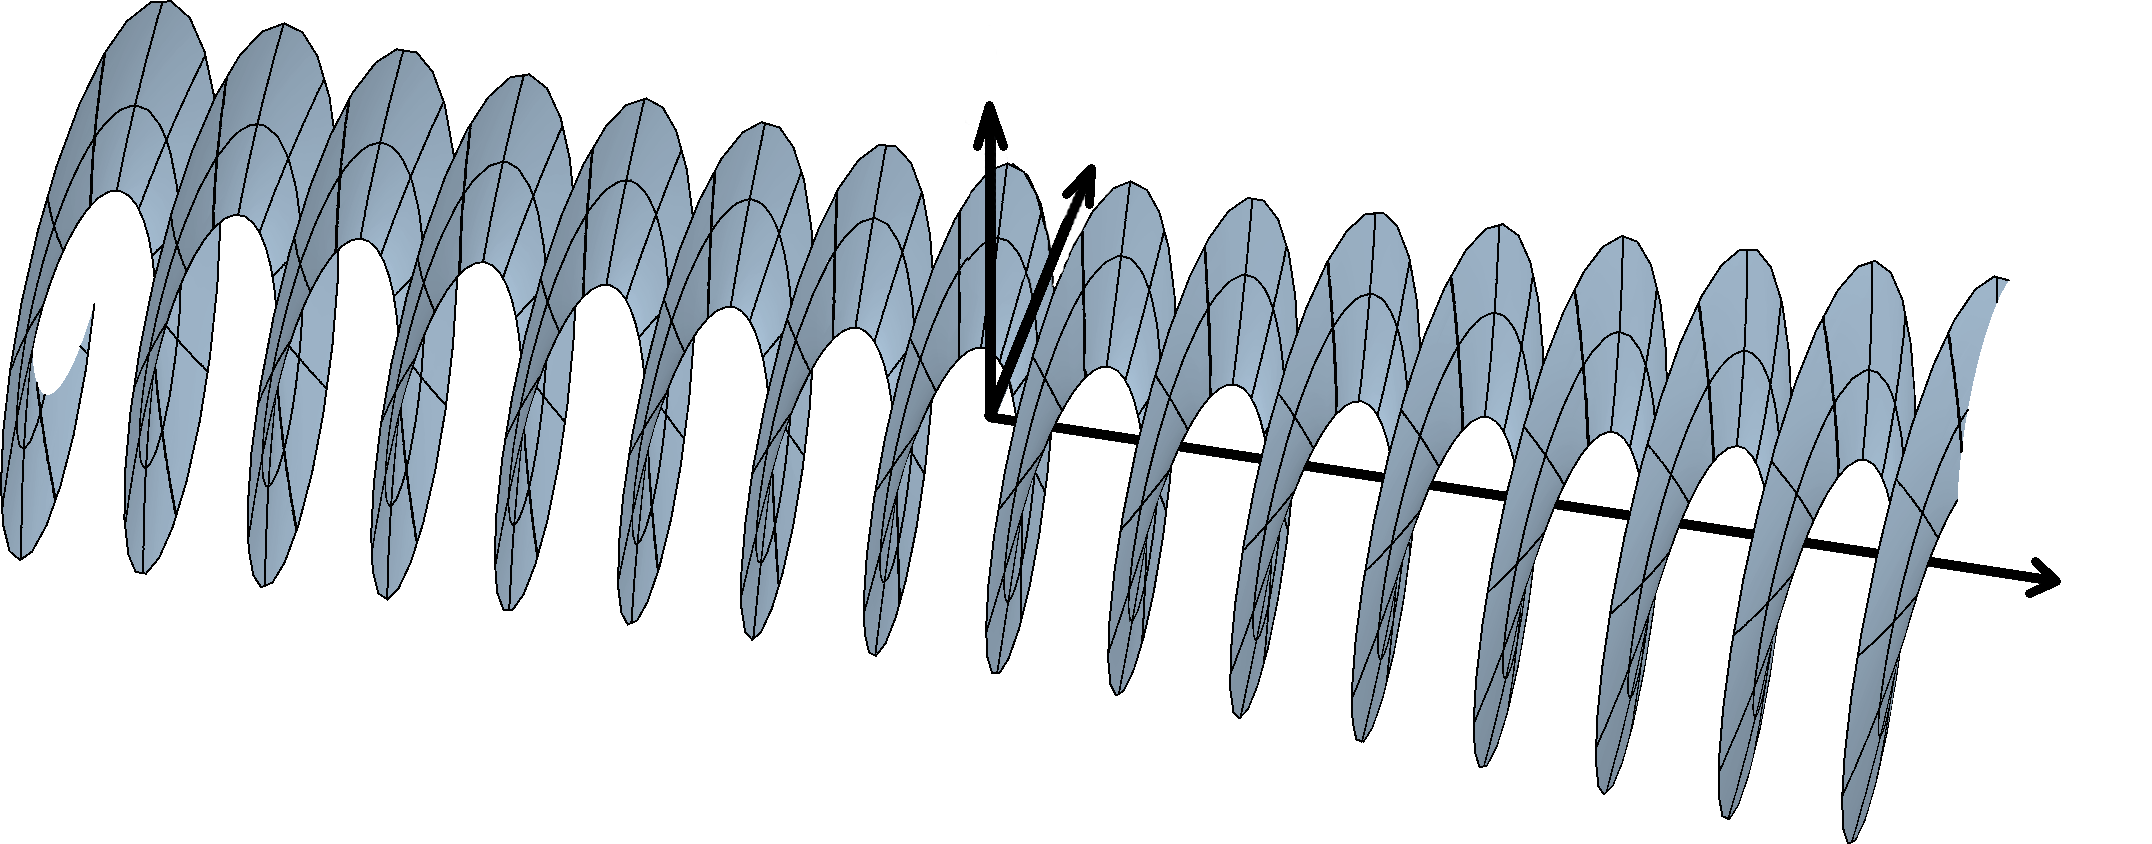
\includegraphics[width=10truecm]{slike/03_Laguerre_faza.png}
\caption{Valovna fronta Laguerre-Gaussovega snopa}
\label{fig:Laguerrova_fronta}
\end{figure}
\end{remark}

\section{*Besslov snop}

Poglejmo še en primer omejenega snopa, to je \index{Besslov snop}Besslov
snop\footnote{Nemški astronom, matematik in fizik Friedrich Wilhelm Bessel, 1784--1846.}. 
Nastavek za rešitev valovne enačbe (enačba~\ref{eq:valovna-skalarna}), 
pri čemer obravnavamo polje skalarno, naj bo
\begin{equation}
E=E_{0}\psi(x,y)e^{i\beta z-i\omega t}.
\end{equation}
Funkcija $\psi$ mora zadoščati Helmholtzevi enačbi\index{Helmholtzeva enačba}
(enačba~\ref{eq:Helmholtz})
\begin{equation}
\nabla_{\perp}^{2}\psi+k_{\perp}^{2}\psi=0
\end{equation}
pri $k_{\perp}^{2}=k^{2}-\beta^{2}$. V cilindričnih
koordinatah ($x=r\cos\varphi$, $y=r\sin\varphi$) se enačba prepiše v 
\begin{equation}
\frac{\partial^2 \psi}{\partial r^2}+ \frac{1}{r}\frac{\partial \psi}{\partial r}
+ \frac{1}{r^2}\frac{\partial^2 \psi}{\partial \varphi^2}+k_{\perp}^{2}\psi=0.
\end{equation}
Rešitve gornje enačbe so s faznim faktorjem pomnožene Besslove funkcije
\begin{equation}
\psi_m(r, \varphi)=J_{m}(k_{\perp}r)e^{im\varphi},
\end{equation}
kjer je $J_{m}$ Besslova funkcija in $m$ celo število. Za
$m=0$ je rešitev osnovi Besslov snop
\begin{equation}
E(r,z,t)=E_{0}J_{0}(k_{\perp}r)e^{i\beta z-i \omega t}.
\label{eq:Besslov-snop}
\end{equation}
Valovne fronte osnovnega Besslovega snopa so ravne
 in njegova divergenca je enaka nič\index{Besslov snop!divergenca}, zato Besslov snop na
poljubni oddaljenosti od izhodišča ohranja svojo obliko. Vendar Besslov snop ni 
omejen v pravem smislu. Za velike oddaljenosti od osi snopa $r$ intenzitetni profil 
namreč pojema kot $I \propto J_{0}^{2}(k_{\perp}r)\sim (2/\pi k_{\perp}r)\cos^{2}(k_{\perp}r-\pi/4)$.
Energija takega snopa ni omejena znotraj efektivnega radija,
kot je to pri Gaussovih snopih. Za konstrukcijo Besslovih snopov
bi (tako kot za konstrukcijo ravnega vala) potrebovali neskončno energije,
kar je seveda nemogoče. Lahko pa ustvarimo dobre približke Besslovih 
snopov, ki imajo pomembne in uporabne lastnosti. 

\begin{figure}[h]
\centering
\def\svgwidth{70truemm} 
\input{slike/03_Bessel_profil.pdf_tex}
\caption{Prečni presek in profil intenzitete Besslovega snopa}
\label{fig:Besslov_presek}
\end{figure}

\begin{remark}
Z uporabo stožčaste leče (aksikona) Gaussov snop
preoblikujemo v približek Besslovega snopa (slika~\ref{fig:Bessel_leca}). 
Na plašču stožčaste leče se namreč Gaussov snop zlomi in valovni vektorji 
nastalega snopa opisujejo stožec, kar je sicer lastnost Besslovih snopov.
Dobljeni snop je na območju z dolžino $z_{max}$ dober približek Besslovega snopa.
Znotraj tega območja je divergenca snopa praktično enaka nič. Poleg manjše divergence
imajo ti snopi še lastnost regeneracije. To pomeni, da se snop 
za objektom, ki ga osvetljuje (na primer v optični pinceti), regenerira. 
Profil snopa na senčni strani (daleč stran od objekta) je tako enak profilu 
snopa pred objektom. 
\begin{figure}[h]
\centering
\def\svgwidth{90truemm} 
\input{slike/03_Bessel_nastanek.pdf_tex}
\caption{Nastanek približka Besslovega snopa na stožčasti leči}
\label{fig:Bessel_leca}
\end{figure}
\end{remark}

\section{Transformacije snopov z lečami}

Vrnimo se k osnovnim Gaussovim snopom in poglejmo, kaj se zgodi z njimi pri prehodu
skozi optične elemente\index{Preslikava z lečo}. Začnemo
z enostavno tanko lečo z goriščno razdaljo $f$. V geometrijski optiki
je krivinski radij krogelnega vala, ki izhaja iz točke na osi, kar
enak razdalji do točke. Leča točko na optični osi preslika v točko na osi,
od koder sledi, da se krogelni val s krivinskim radijem $R_{1}$
po prehodu skozi lečo spremeni v val s krivinskim radijem $R_{2}$.
Pri tem velja zveza 
\begin{equation}
\frac{1}{R_{1}}-\frac{1}{R_{2}}=\frac{1}{f}.
\label{eq:leca}
\end{equation}
Dogovorimo se, da je krivinski radij v točki $z$ pozitiven, če je središče krožnice pri $z^{\prime}\le z$.

Kako pa je z Gaussovim snopom? Polmer snopa $w$ se pri prehodu 
skozi tanko lečo ne spremeni, zato velja po enačbah (\ref{eq:q-inv}) in 
(\ref{eq:leca}) za kompleksni krivinski radij tik pred lečo in tik za njo
\begin{equation}
\frac{1}{q_{1}}-\frac{1}{q_{2}}=\frac{1}{f}.
\label{eq:preslikava-zveza-leca}
\end{equation}
Kompleksni krivinski radij $q$ je po enačbi~(\ref{eq:q}) linearna 
funkcija koordinate $z$ in za opis Gaussovega snopa zadošča, da
v neki točki $z$ poznamo $q$. Iz realnega dela parametra $q$ določimo ukrivljenost front in iz 
imaginarnega polmer snopa. Enačba~(\ref{eq:preslikava-zveza-leca}) torej
zadošča za račun prehoda snopa skozi poljuben sistem leč brez aberacij, če le poznamo
njegovo goriščno razdaljo.

Kot primer poglejmo, kako z zbiralno lečo zberemo Gaussov snop.
\begin{figure}[h]
\centering
\def\svgwidth{140truemm} 
\input{slike/03_preslikava.pdf_tex}
\caption{Prehod Gaussovega snopa skozi
tanko lečo. Grlo velikosti $w_{01}$ v oddaljenosti $x_{1}$ od gorišča
leče $F$ se preslika v grlo velikosti $w_{02}$ v oddaljenosti $x_{2}$ od gorišča
leče $F$.}
\label{fig:Prehod-Gaussovega-snopa}
\end{figure}

Vpadni snop naj ima grlo s polmerom $w_{01}$ in parametrom $z_{01}=\pi w_{01}^2/\lambda$. 
Grlo naj leži v točki, ki je za $x_{1}$ oddaljena od levega gorišča leče $F$ (slika
\ref{fig:Prehod-Gaussovega-snopa}). Naj bosta 
\begin{equation}
q_{1}^{F}=x_{1}-iz_{01}\mbox{\hskip1cm in \hskip1cm}q_{2}^{F}=-x_{2}-iz_{02}
\label{eq:qFqF}
\end{equation}
 kompleksna krivinska radija v levem in desnem gorišču, pri čemer je koordinatna os $z$ 
 usmerjena v desno, gledamo pa referenčno glede na lego grla vsakega posameznega snopa. 
 Za vrednosti $q$ tik pred lečo in tik za njo velja tudi
\begin{equation}
q_{1}=q_{1}^{F}+f\mbox{\hskip1cm in \hskip1cm}q_{2}=q_{2}^{F}-f.
\end{equation}
 Od tod z uporabo enačbe~(\ref{eq:preslikava-zveza-leca}) izpeljemo zvezo
za $q$ v goriščih v kompaktni obliki 
\boxeq{eq:qqf}{
q_{1}^{F}q_{2}^{F}=-f^{2}.
}
Uporabimo enačbi~(\ref{eq:qFqF}) in 
zapišemo posebej realni in imaginarni del 
\begin{equation}
x_{1}x_{2}=f^{2}-z_{01}z_{02} \qquad \mathrm{in} \qquad
\frac{x_{1}}{z_{01}}=\frac{x_{2}}{z_{02}}.
\end{equation}
Dobimo enačbi za preslikavo Gaussovega snopa z lečo z goriščno razdaljo $f$.
Prva enačba določa lego grla preslikanega snopa na desni strani leče
\boxeq{eq:preslikava-grlo}{
x_{2}=\frac{x_{1}f^{2}}{x_{1}^{2}+z_{01}^{2}}.
}
Druga enačba določa povečavo
\boxeq{eq:preslikava-povecava}{
\frac{w_{02}}{w_{01}}=\sqrt{\frac{x_{2}}{x_{1}}}.
}
Enačba (\ref{eq:preslikava-grlo}) se ujema z izrazom za preslikavo točke v geometrijski
optiki le, kadar je $z_{01}\ll x_{1}$. Kadar je $z_{01}\gg f$, je
val na leči skoraj raven in $x_2 \to 0$, kar pomeni, da leži
grlo na desni strani v gorišču. V praksi za Gaussove snope, ki izhajajo iz laserjev, pogosto ne
velja ne prva ne druga limita, zato je treba uporabiti zapisani izraz 
(enačba~\ref{eq:preslikava-grlo}).
Tudi velikost polmera grla na desni, podana z enačbo (\ref{eq:preslikava-povecava}),
je precej drugačna kot v geometrijski optiki.

Za primer vzemimo snop iz He-Ne laserja\index{Laser!He-Ne} z valovno dolžino 
$633~\si{\nano\metre}$. Grlo snopa naj leži na izhodu iz laserja, njegov polmer naj bo 
$w_{01}=0,5~\si{\milli\metre}$. Za tak snop je $z_{01}=124~\si{\centi\metre}$. 
Na oddaljenost $50~\si{\centi\metre}$ od grla postavimo lečo z goriščno razdaljo 
$f=25~\si{\centi\metre}$. Po enačbi (\ref{eq:preslikava-grlo})
leži grlo za lečo v oddaljenosti $1~\si{\centi\metre}$ od gorišča in torej $26~\si{\centi\metre}$ 
za lečo. Izračunan polmer je po enačbi~(\ref{eq:preslikava-povecava})
$w_{02}=100~\si{\micro\metre}$. Enačbe geometrijske optike bi
dale popolnoma napačen položaj grla $50~\si{\centi\metre}$ za lečo in polmer grla  
$0,5~\si{\milli\metre}$. Po drugi strani bi približek, da je vpadni
snop kar raven, dal grlo na desni v gorišču s približno pravim polmerom. Zakaj da približek ravnih 
valov bolj pravilen rezultat, hitro uvidimo, če pogledamo
Rayleighovo dolžino snopa $z_{01}$: 
snop vpada na lečo še v območju bližnjega polja ($x_1 + f < z_{01}$), znotraj katerega
ima približno obliko ravnih valov. 

Če postavimo gorišče leče v grlo snopa ($x_{1}=0$), je grlo na
desni strani tudi v gorišču ($x_{2}=0$). Razmerje polmerov grl
na eni in drugi strani leče izračunamo
\begin{equation}
\lim_{x_1 \to 0}~\frac{x_{2}}{x_{1}}=\frac{f^{2}}{z_{01}^{2}} \qquad \textrm{in} \qquad
\frac{w_{02}}{w_{01}}= \frac{f}{z_{01}}.\index{Gaussov snop!grlo}
\end{equation}
Velikost grla na desni strani je tako
\begin{equation}
w_{02}=\frac{\lambda f}{\pi w_{01}}.
\end{equation}
Če želimo doseči kar se da majhno grlo po prehodu skozi lečo, mora biti polmer
vpadnega snopa kar se da velik. Vpadni snop je tako smiselno
razširiti, vendar polmer snopa ne more biti večji od polmera leče $a$. 
Najmanjša velikost grla, ki jo še lahko dosežemo z zbiralno lečo, je tako 
\boxeq{eq:wmin}{
w_{02~\textrm{min}} = \frac{\lambda f}{\pi a} \sim \lambda.
}
Dobri mikroskopski in fotografski
objektivi dosegajo $f/a\simeq 1$, zato je mogoče z njimi Gaussov snop
zbrati v piko velikosti $\sim\lambda$. 

Omenili smo, da je treba za dosego majhnega polmera grla za lečo snop pred lečo čim bolj razširiti.
Razširitev vpadnega snopa naredimo s teleskopom~(slika~\ref{fig:Prehod-Gaussovega-snopa-teleskop}),
katerega značilnost je, da je razmik med lečama enak vsoti goriščnih razdalj leč in zato gorišči
sovpadata. Povečava teleskopa je pri taki postavitvi enaka razmerju med goriščnima razdaljama leč
(glej nalogo~\ref{teleskop}).

\begin{figure}[h]
\def\svgwidth{145truemm} 
\input{slike/03_teleskop.pdf_tex}
\caption{Prehod Gaussovega snopa
skozi teleskop iz leč z goriščnima razdaljama $f_{1}$ in $f_{2}$}
\label{fig:Prehod-Gaussovega-snopa-teleskop}
\end{figure}

\begin{definition}
\label{teleskop}
Dve leči z goriščnima razdaljama $f_{1}$ in $f_{2}$ naj bosta na medsebojni
razdalji $d=f_{1}+f_{2}$. Pokaži, da je povečava takega teleskopa enaka  
\begin{equation}
\frac{w_{02}}{w_{01}}=\frac{f_{2}}{f_{1}}.
\label{eq:povecava-teleskop}
\end{equation}
\end{definition}

\section{Matrične (ABCD) preslikave v geometrijski optiki}

Preden se lotimo splošnejšega zapisa preslikav Gaussovega snopa, 
se spomnimo, kako obravnavamo preslikave v geometrijski optiki. 
Slika nastane kot presečišče žarkov,
ki izhajajo iz točke predmeta pred optičnim sistemom. Žarek 
je pravokoten na valovne ploskve, pri čemer moramo vzeti še limito zelo majhne
valovne dolžine. Ukrivljenost valovne fronte je neposredno
povezana s spreminjanjem naklona žarkov, pri čemer bomo privzeli, da so 
nakloni žarkov glede na os majhni.

Žarek v izbrani ravnini $z$ opišemo z dvema parametroma: 
oddaljenostjo $y$ od osi in naklonom $\vartheta$ glede na os sistema. Ti dve količini 
sta med seboj neodvisni in ju sestavimo 
v vektor
\begin{equation}
\left[\begin{array}{c}
y\\
\vartheta
\end{array}\right].
\end{equation}
Preslikavo žarka zapišemo kot matriko, ki deluje na vpadni vektor in ga preslika
v izhodni vektor (slika~\ref{fig:K-matricni-obravnavi})
\begin{equation}
\left[\begin{array}{c}
y_2\\
\vartheta_2
\end{array}\right] = M \left[\begin{array}{c}
y_1\\
\vartheta_1
\end{array}\right].
\end{equation}

\begin{figure}[h]
\centering
\centering
\def\svgwidth{100truemm}
\input{slike/03_k_preslikavam.pdf_tex}
\caption{Preslikave žarkov lahko obravnavamo
z matrikami. Optični element, ki ga predstavlja matrika $M$, 
preslika žarek $(y_{1},\vartheta_{1})$
v $(y_{2},\vartheta_{2})$.}
\label{fig:K-matricni-obravnavi}
\end{figure}

Matrike $M$ so na splošno oblike
\begin{equation}
M = \left[\begin{array}{cc}
A & B\\
C & D
\end{array}\right],
\label{eq:ABCDdef}
\end{equation}
zato jih imenujemo matrike ABCD\index{Matrike ABCD}. Poglejmo nekaj primerov. 

Pri premiku za $d$ vzdolž osi se zaradi končnega naklona spremeni odmik od osi, naklon pa ostane enak
\begin{equation}
\left[\begin{array}{c}
y_{2}\\
\vartheta_{2}
\end{array}\right]=\left[\begin{array}{c}
y_{1}+d\vartheta_{1}\\
\vartheta_{1}
\end{array}\right].
\end{equation}
To zapišemo v matrični obliki
\begin{equation}
\left[\begin{array}{c}
y_{2}\\
\vartheta_{2}
\end{array}\right]=\left[\begin{array}{cc}
1 & d\\
0 & 1
\end{array}\right]\cdot\left[\begin{array}{c}
y_{1}\\
\vartheta_{1}
\end{array}\right].
\end{equation}
Matrika za premik $d$ vzdolž osi $z$ je tako
\begin{equation}
M= \left[\begin{array}{cc}
1 & d\\
0 & 1
\end{array}\right].
\label{eq:MABCD1}
\end{equation}
Poglejmo še matriko za prehod skozi lečo. 
Pri prehodu skozi tanko lečo se spremeni nagib žarka. Če je žarek pred
lečo vzporeden z osjo, gre za lečo skozi gorišče, zato 
\begin{equation}
\left[\begin{array}{c}
y_{2}\\
\vartheta_{2}
\end{array}\right]=\left[\begin{array}{c}
y_{1}\\
-\frac{y_{1}}{f}
\end{array}\right]=\left[\begin{array}{cc}
1 & B\\
-\frac{1}{f} & D
\end{array}\right]\cdot\left[\begin{array}{c}
y_{1}\\
0
\end{array}\right].
\end{equation}
Pri tem koeficientov $B$ in $D$ še ne poznamo. Določimo jih iz drugega pogoja, 
ki pravi, da se žarek, ki gre skozi lečo na osi, ne spremeni
\begin{equation}
\left[\begin{array}{c}
y_{2}\\
\vartheta_{2}
\end{array}\right]=\left[\begin{array}{c}
0\\
\vartheta_{1}
\end{array}\right]=\left[\begin{array}{cc}
1 & B\\
-\frac{1}{f} & D
\end{array}\right]\cdot\left[\begin{array}{c}
0\\
\vartheta_{1}
\end{array}\right].
\end{equation}
 Sledi $B=0$ in $D=1$. Matrika za prehod skozi lečo je tako 
\begin{equation}
M= \left[\begin{array}{cc}
1 & 0\\
-\frac{1}{f} & 1
\end{array}\right].
\label{eq:MABCD2}
\end{equation}
Podobno izpeljavo kot za prehod skozi lečo naredimo za odboj na sferičnem zrcalu
s krivinskim radijem $R$. Pripadajoča matrika je 
\begin{equation}
M=\left[\begin{array}{cc}
1 & 0\\
-\frac{2}{R} & 1
\end{array}\right],
\end{equation}
pri čemer je $R>0$ za konkavna zrcala. Matrika za odboj na ravnem zrcalu je identiteta.

Matriko sestavljene optične naprave zapišemo kot produkt matrik posameznih komponent. 
Pri tem moramo paziti na vrstni red množenja, saj množenje matrik ni komutativno.
Matriko preslikave z dvema optičnima elementoma, pri čemer žarek 
najprej preide element z indeksom 1 in nato element z indeksom 2, zapišemo kot 
\begin{align}
\left[\begin{array}{cc}
A & B\\
C & D
\end{array}\right] & =  \left[\begin{array}{cc}
A_{2} & B_{2}\\
C_{2} & D_{2}
\end{array}\right]\cdot\left[\begin{array}{cc}
A_{1} & B_{1}\\
C_{1} & D_{1}
\end{array}\right].
\end{align}
V sistemu z več elementi zapišemo produkt matrik za vse elemente, 
vendar ne smemo pozabiti na premike med posameznimi elementi.

Poglejmo primer. Žarek naj najprej prepotuje razdaljo $d$, nato ga usmerimo
na tanko lečo z goriščno razdaljo $f$. Matrika za celoten prehod je
\begin{align}
\left[\begin{array}{cc}
A & B\\
C & D
\end{array}\right] & =  \left[\begin{array}{cc}
1 & 0\\
-\frac{1}{f} & 1
\end{array}\right]\cdot\left[\begin{array}{cc}
1 & d\\
0 & 1
\end{array}\right] =  \left[\begin{array}{cc}
1 & d\\
-\frac{1}{f} & -\frac{d}{f}+1
\end{array}\right].
\label{eq:Mdf}
\end{align}
\begin{remark}
Opisani matrični formalizem je zelo prikladen predvsem za računanje prehoda
svetlobe skozi zapletene optične sisteme, saj ga je prav lahko izvesti z računalnikom. Poleg
tega je enolično povezan z matričnim formalizmom za izračun
kompleksne ukrivljenosti Gaussovih snopov, zato omogoča preprost prenos 
rezultatov geometrijske optike v optiko Gaussovih snopov.
\end{remark}

\section{Linearne racionalne transformacije kompleksnega krivinskega radija}

Poskusimo zapisati podoben formalizem za kompleksne krivinske
radije. Za opis Gaussovega snopa zadošča, da v izbrani ravnini $z$ poznamo kompleksni
krivinski radij $q$. Vemo, da je $q$ linearna funkcija
premika po $z$ (enačba~\ref{eq:q}), in vemo, kako se $q$ 
spremeni pri prehodu skozi tanko lečo (enačba~\ref{eq:preslikava-zveza-leca}). 

Pri premiku iz ravnine $z_1$ v ravnino $z_2$, ki je od prve oddaljena
za $d$, se $q$ spremeni 
\begin{equation}
q_2=q_1+d.
\end{equation}
Po enačbi~(\ref{eq:preslikava-zveza-leca}) je pri prehodu skozi lečo
\begin{equation}
q_2=\frac{q_1f}{f-q_1}=\frac{q_1}{-\frac{q_1}{f}+1}.
\end{equation}
Premik in leča dasta skupaj
\begin{equation}
q_2=\frac{q_1+d}{-\frac{q_1+d}{f}+1}=\frac{q_1+d}{-\frac{q_1}{f}-\frac{d}{f}+1}.
\label{eq:premikleca}
\end{equation}
V vseh treh primerih smo transformacijo kompleksnega krivinskega radija 
$q$ zapisali v obliki ulomljene linearne oziroma M\"obiusove 
preslikave
\boxeq{eq:ulomljena-preslikava}{
q_2=\frac{Aq_1+B}{Cq_1+D}.
}
Ko koeficiente preslikave razvrstimo v matriko 
\begin{equation}
M= \left[\begin{array}{cc}
A & B\\
C & D
\end{array}\right]
\end{equation}
in iz gornjih enačb razberemo koeficiente matrik \index{Matrike ABCD} za opisane 
preslikave, vidimo, da so povsem enaki koeficientom matrik ABCD, ki jih poznamo iz
geometrijske optike (\ref{eq:MABCD1}, \ref{eq:MABCD2} in \ref{eq:Mdf}). Matrike, ki jih
poznamo iz geometrijske optike, lahko torej uporabimo tudi za izračun preslikave snopov,
vendar v tem primeru elemente matrike razvrstimo v ulomljeno linearno preslikavo.

Omenimo še eno lastnost matrik ABCD. Kadar po prehodu skozi optične elemente snop svetlobe 
preide v snov z enakim lomnim količnikom, kot je bil na začetku, je determinanta matrike 
ABCD enaka 1. V nasprotnem
primeru je determinanta matrike enaka razmerju lomnih količnikov začetne in končne snovi. 
\begin{equation}
\det(M) = AD-BC = \frac{n_1}{n_2}.
\end{equation}
\newpage
\begin{table}[t!]
 \centering
  \begin{tabular}{|c|c|c|} \hline
  Opis prehoda & Skica & Matrika za prehod \\ \hline   
      Prehod skozi prostor za $d$ & \parbox[c]{3cm}{\def\svgwidth{3cm}\input{slike/03_matrika_d.pdf_tex}} & 
      $\begin{bmatrix} 1 & d\\  0 & 1 \end{bmatrix}$ \\ \hline

      Prehod skozi mejo dveh snovi & \parbox[c]{3cm}{\def\svgwidth{3cm}\input{slike/03_matrika_n.pdf_tex}} & 
      $\begin{bmatrix} 1 & 0\\ 0 & \frac{n_{1}}{n_{2}} \end{bmatrix}$ \\ \hline
      
      Prehod skozi konveksno ukrivljeno mejo $R>0$ & \parbox[c]{3cm}{\def\svgwidth{3cm}\input{slike/03_matrika_nR.pdf_tex}} & 
      $\begin{bmatrix} 1 & 0\\ \frac{(n_{1}-n_{2})}{n_{2}R} & \frac{n_{1}}{n_{2}} \end{bmatrix}$ \\ \hline
      
      Prehod skozi konveksno lečo $f>0$ & \parbox[c]{3cm}{\def\svgwidth{3cm}\input{slike/03_matrika_f.pdf_tex}} & 
      $\begin{bmatrix} 1 & 0\\ -\frac{1}{f} & 1 \end{bmatrix}$ \\ \hline
      
      Odboj na konkavnem zrcalu $R>0$ & \parbox[c]{3cm}{\def\svgwidth{3cm}\input{slike/03_matrika_R.pdf_tex}} & 
      $\begin{bmatrix} 1 & 0\\ -\frac{2}{R} & 1 \end{bmatrix}$ \\ \hline    
  \end{tabular}
  \caption{Matrike ABCD za nekaj osnovnih preslikav, ki veljajo tako v 
	  geometrijski optiki kot za izračun preslikave kompleksnega
	  krivinskega radija $q$ Gaussovih snopov}
\label{fig:Matrike-za-preslikave}
\end{table}

\begin{definition}
Pokaži, da za naslednje prehode veljajo ustrezne matrike ABCD. \\ \\
\begin{tabular}{|c|c|c|} \hline  
      Prehod skozi prostor in lečo & \parbox[c]{3cm}{\def\svgwidth{3cm}\input{slike/03_matrika_df.pdf_tex}} & 
      $\begin{bmatrix} 1 & d\\ -\frac{1}{f} & 1-\frac{d}{f} \end{bmatrix}$ \\ \hline
      \parbox[c]{12em}{Prehod skozi lečo z debelino $d$ 
      in krivinskima radijema $R_1$ in $R_2$}& 
      \parbox[c]{3cm}{\def\svgwidth{3cm}\input{slike/03_matrika_fd.pdf_tex}} & 
      $\begin{bmatrix} 1-\frac{d}{nf_{1}} & \frac{d}{n}\\
      -\frac{1}{f_2}- \frac{1}{f_1}-\frac{d}{nf_1f_2}& 1-\frac{d}{nf_{2}} \end{bmatrix}$
      $f_{i}=\frac{R_{i}}{n-1}$\\ \hline
      Prehod skozi zaporedje plasti & \parbox[c]{3cm}{\def\svgwidth{3cm}\input{slike/03_matrika_nN.pdf_tex}} & 
      $\begin{bmatrix} 1 & \sum_{i=1}^{N}\frac{d_{i}}{n_{i}}\\ 0 & 1 \end{bmatrix}$ \\ \hline 
\end{tabular}
\end{definition}

%Final

%-------------------------------------------------------------------------------
%	CHAPTER 4
%-------------------------------------------------------------------------------

%\chapterimage{Resonator.jpg} % Chapter heading image

\chapter{Optični resonatorji}
Osnovni gradnik vsakega laserja je resonator. V njem je vzbujeno lastno elektromagnetno
nihanje, ki skozi delno prepustno steno resonatorja kot valovanje
izhaja iz sistema. V tem poglavju bomo 
spoznali različne vrste optičnih resonatorjev in kriterije za njihovo stabilno delovanje,
izračunali lastne frekvence resonatorjev in povezali izgube v laserskem resonatorju s
spektralno širino izsevane svetlobe.

\section{Odprti resonatorji}
Optični resonatorji\index{Resonator} so votline, v katerih je mogoče 
vzpostaviti stoječe svetlobno\index{Stoječe valovanje} valovanje. Če vzbujamo v resonatorju valovanja z 
različnimi frekvencami, se pri nekaterih diskretnih frekvencah pojavi resonančno
obnašanje. Te frekvence imenujemo lastne frekvence\index{Lastne frekvence resonatorja}
resonatorja in stoječa valovanja lastna nihanja. Zaradi dušenja imajo lastna nihanja
v resonatorju končno frekvenčno oziroma spektralno 
širino. Pri tem je čas dušenja mnogo daljši od nihajne periode. 

Optične resonatorje uporabljamo predvsem v dva namena:
\begin{enumerate}
\item V resonatorjih se ob razmeroma šibkem zunanjem vzbujanju pojavi velika jakost
električnega polja pri resonančni frekvenci. Za vzdrževanje
konstantne amplitude lastnega nihanja mora zunanji vir zgolj pokrivati izgube. 
Če so te majhne, je zunanji vir lahko šibek in polje
v resonatorju vseeno veliko.
\item Resonatorji delujejo kot filtri, ki prepuščajo le polje s točno  
določeno frekvenco in izbrano prostorsko odvisnostjo. Primer take uporabe je 
Fabry-Perotov interferometer\index{Fabry-Perotov interferometer}. 
\end{enumerate}

\begin{remark}
Poleg optičnih resonatorjev poznamo resonatorje tudi na drugih področjih, 
na primer akustične resonatorje pri glasbilih ali mikrovalovne in radijske resonatorje. 
V mikrovalovnem področju, kjer so valovne dolžine valovanja
okoli $1~\si{\centi\metre}$, 
so resonatorji zaprte kovinske votline z dimenzijami, ki so primerljive z 
valovno dolžino vzbujenega valovanja. Resonančne frekvence so v takem resonatorju 
med seboj dobro ločene in ni težko vzbuditi enega samega lastnega nihanja na izbranem 
frekvenčnem intervalu.
\end{remark}

V optiki so resonatorji navadno veliko večji
od valovne dolžine svetlobe. Vzemimo kocko s stranico $L\gg \lambda$, 
v kateri je vzbujeno zelo veliko število lastnih nihanj. Število lastnih nihanj $N$ 
na frekvenčni interval $\Delta \nu$ zapišemo z zvezno gostoto 
stanj\index{Gostota stanj}\footnote{Glej npr. B. E. A. Saleh in M. C. Teich, 
{\it Fundamentals of Photonics}, druga izdaja, John Wiley \& Sons, Inc. (2007).}
\begin{equation}
N=2 \frac{1}{8} 4\pi k^{2}\Delta k \frac{1}{(\pi/L)^3}=\frac{\omega^{2}}{\pi^{2}c^{3}}V\Delta\omega=
\frac{8\pi \nu^{2}}{c^{3}}V\Delta\nu.
\label{eq:N-stevilo-stanj}
\end{equation}
Do enačbe smo prišli tako, da smo prešteli stoječa valovanja z velikostjo
valovnega vektorja med $k$ in $k+\Delta k$: volumen pripadajoče krogelne lupine v pozitivnem oktantu
$\frac{1}{8} 4\pi k^{2}\Delta k$ smo delili z volumnom $(\pi/L)^3$, ki pripada enemu stanju. 
Upoštevali smo tudi, da ima vsako lastno nihanje lahko dve polarizaciji.

Poglejmo primer. Izberimo osrednjo frekvenco $\nu=3\cdot10^{14}~\si{\hertz}$, ki
ustreza valovni dolžini $1~\si{\micro\metre}$, in širino frekvenčnega
intervala $\Delta\nu=3\cdot10^{9}~\si{\hertz}$, ki je značilna za Dopplerjevo
razširjeno emisijsko črto v plinu\index{Dopplerjeva razširitev}. 
Potem je v votlini s stranico $L=1~\si{\centi\metre}$ 
in prostornino $V=1~\si{\centi\metre^3}$ število lastnih nihanj na izbran frekvenčni interval 
po enačbi~(\ref{eq:N-stevilo-stanj}) enako
$N=2,5\cdot10^{8}$. Če bi bile vse stene votline idealna zrcala,
bi bil čas dušenja vseh lastnih nihanj približno enako dolg in vedno bi vzbujali
zelo veliko število resonanc hkrati. Tak resonator bi bil neuporaben.

Hkratnemu vzbujanju velikega števila lastnih nihanj se izognemo z zmanjšanjem odbojnosti
stranskih sten votline, saj tako povečamo dušenje valov v prečni smeri.
Dušenje valov, pravokotnih na idealno odbojni končni steni, ostane nespremenjeno.
Nazadnje lahko stranske stene odstranimo, tako da stoječih valov v prečni smeri
sploh ni več. Ostane le še nekaj valov, ki so pravokotni na končni
steni. Resonatorju brez stranskih sten  pravimo odprti resonator\index{Resonator!odprti} 
(slika~\ref{fig:Odprt_resonator}).
\begin{figure}[h]
\centering
\def\svgwidth{110truemm} 
\input{slike/04_Odprt_resonator.pdf_tex}
\caption{Lastni nihajni načini odprtega resonatorja imajo diskretne vrednosti
velikosti valovnih vektorjev (a). Žarki, ki niso pravokotni na zrcali, 
iz odprtega resonatorja uidejo (b).}
\label{fig:Odprt_resonator}
\end{figure}

Obravnavajmo odprte resonatorje podrobneje. V zaprti pravokotni votlini velikosti
$a\times a\times L$ z idealno odbojnimi stenami so vrednosti
valovnega vektorja za lastna nihanja \index{Valovni vektor}
\begin{equation}
\mathbf{k}_{l,m,n}=\left(\frac{l\pi}{a}\,,\frac{m\pi}{a}\,,\frac{n\pi}{L}\right),\label{eq:k-votlina}
\end{equation}
kjer so $l$, $m$ in $n$ cela števila, $L$ dolžina in $a$ prečna
dimenzija resonatorja. Lastne krožne frekvence resonatorja so 
\begin{equation}
\omega_{l,m,n}=c|\mathbf{k}_{l,m,n}|.\label{eq:omega-votlina}
\end{equation}
Ker je dolžina resonatorja $L$ velika v primerjavi z $\lambda$, je $n$
zelo veliko število. Če prečnih sten ni, je  $\mathbf{k}$ približno
vzporeden z osjo $z$ in števili $l$ in $m$ sta majhni. Tedaj
lahko velikost valovnega vektorja razvijemo in krožno frekvenco zapišemo kot
\begin{equation}
\omega_{l,m,n}=c\left(\frac{n\pi}{L}+\frac{l^{2}+m^{2}}{2n}\frac{L \pi}{a^{2}}\right).
\label{eq:delta-omega-resonator-razvoj}
\end{equation}
Drugi člen v oklepaju je le majhen popravek, tako da so
lastne frekvence odprtih optičnih resonatorjev odvisne predvsem od
števila vozlov v vzdolžni smeri. To število je navadno veliko, med $10^{5}$
in $10^{7}$. Mogoča so tudi lastna nihanja z nekaj vozli v prečni
smeri, ki pa navadno le malo vplivajo na lastne frekvence. V nadaljevanju
bomo obravnavali predvsem lastna nihanja brez vozlov v prečni smeri in
jih označili z enim samim indeksom $n$.

Razlika med frekvencama dveh zaporednih lastnih nihanj\index{Lastne frekvence resonatorja} 
$n$ in $n+1$ je
\boxeq{eq:delta-omega-resonator}{
\Delta\omega_n=\frac{\pi c}{L} \qquad \mathrm{oziroma} \qquad \Delta \nu_n = \frac{c}{2L}.
}
Pri dolžini resonatorja $L=30~\si{\centi\metre}$ je v frekvenčnem
intervalu $\Delta \nu = 3\cdot10^{9}~\si{\hertz}$ le še $\Delta \nu /\Delta \nu_n = 6$ lastnih 
nihanj, ki jih je brez težav mogoče razločiti.

V zaprtih votlinah z zrcalnimi stenami obstajajo dobro določena lastna
nihanja pri poljubni obliki votline. To ne drži za odprte resonatorje.
Da se pojavijo lastna nihanja z majhnimi izgubami, morata
biti izpolnjena dva pogoja:

\begin{enumerate} 
\item Snop žarkov mora po mnogih odbojih ostati ujet med zrcaloma resonatorja.
\item Polmer zrcala mora biti večji od polmera uklonsko razširjenega snopa, ki se širi od nasprotnega zrcala. 
\end{enumerate}

Resonatorje, ki zadoščajo zapisanima pogojema, imenujemo stabilni 
resonatorji\index{Stabilnost resonatorja}.
Drugi pogoj lahko zapišemo tudi z enačbo, izhajajoč iz enačbe za oceno divergence (enačba~\ref{eq:kot_ocena}):
\begin{equation}
a_2 > L \vartheta = L\frac{\lambda}{a_1}\qquad \mathrm{oziroma} \qquad
\frac{a_{1}a_{2}}{\lambda L}>1,
\label{eq:Fresnelovo_stevilo}
\end{equation}
kjer sta $a_{1}$ in $a_{2}$ polmera zrcal. Izrazu 
$
F = a_{1}a_{2}/\lambda L
$
pravimo Fresnelovo število\index{Fresnelovo število} (enačba~\ref{eq:Fst})
in resonator je stabilen za $F>1$. Laserji imajo pogosto $F\gg 1$, lahko tudi $F \sim 100$, zato je 
prvi kriterij navadno odločujoč pri ugotavljanju stabilnosti resonatorja.

\subsection*{Fabry-Perotov interferometer}
Poglejmo resonator, omejen z dvema vzporednima ravnima zrcaloma
z veliko odbojnostjo. Takemu sistemu pravimo \index{Fabry-Perotov 
interferometer}Fabry-Perotov 
interferometer\footnote{Francoska fizika Maurice Paul Auguste Charles Fabry, 1867--1945, in 
Jean-Baptiste Alfred Perot, 1863--1925.}. 
Da nastane med zrcaloma stoječe valovanje, mora biti razdalja 
med zrcaloma večkratnik polovične valovne dolžine (enačba~\ref{eq:k-votlina})
\begin{equation}
L = \frac{n \lambda}{2}.
\end{equation}
Prepustnost interferometra za ravni val, ki vpada pravokotno na zrcali z
odbojnostjo ${\cal R}$, lahko izračunamo (glej nalogo~\ref{naloga:FP}). Prepustnost, to je 
razmerje med intenzitetama prepuščenega in vpadnega valovanja, je odvisna
od  frekvence vpadnega valovanja
\begin{equation}
T=\frac{I}{I_0} = \frac{1}{1+\frac{4{\cal R}}{(1-{\cal R})^{2}}\sin^{2}\omega L/c}
\label{eq:Fabry-Perot-prepustnost}
\end{equation}
in je prikazana na sliki~\ref{fig:Fabry-Perot} za tri različne vrednosti ${\cal R}$.
\begin{figure}[h!]
\centering
\def\svgwidth{95truemm} 
\input{slike/04_fabry_perot.pdf_tex}
\caption{
Prepustnost Fabry-Perotovega interferometra $T$
v odvisnosti od frekvence vpadnega valovanja $\nu$ pri različnih odbojnostih zrcal ${\cal R}$}
\label{fig:Fabry-Perot}
\end{figure}

Ko je frekvenca vpadnega valovanja enaka lastni frekvenci
resonatorja, je sistem v resonanci in $T=1$. Pri drugih frekvencah je prepustnost znatno manjša, predvsem
pri velikih $\cal{R}$, kjer pade praktično na nič. Z naraščajočo odbojnostjo zrcal ${\cal R}$ 
se zmanjšuje tudi širina resonančnega vrha.
\begin{naloga}
\label{naloga:FP}
Pokaži, da je prepustnost Fabry-Perotovega interferometra, katerega zrcali imata odbojnost $\cal{R}$, enaka 
\begin{equation}
T = \frac{1}{1+\frac{4\cal{R}}{(1-{\cal R})^2}\sin^2 \delta},
\label{eq:FP}
\end{equation}
kjer je $\delta = kL\cos{\vartheta}$, $L$ razmik med zrcaloma, $\vartheta$ vpadni kot in
$k$ valovno število.
\end{naloga}

Prvemu pogoju za stabilnost ustrezajo v Fabry-Perotovem interferometru
le žarki, ki so natanko pravokotni na zrcali. Čim sta zrcali le
malo nevzporedni, stabilnih žarkov sploh ni več. Tak 
planparalelni interferometer\index{Resonator!planparalelni} torej deluje 
na meji stabilnosti. Z izpolnjevanjem drugega
pogoja ni težav, saj morata biti pri na primer $30~\si{\centi\metre}$ dolgem resonatorju in 
valovni dolžini $0,5~\si{\micro\metre}$ zrcali večji od $0,4~\si{\milli\metre}$, da zadostita pogoju, 
zapisanem v enačbi~(\ref{eq:Fresnelovo_stevilo}).

\section{Gaussovi snopi v resonatorjih}
Spoznali smo planparalelni resonator, ki deluje na meji stabilnosti. 
Bolj stabilni resonatorji so sestavljeni iz dveh konkavno ukrivljenih
zrcal. V njih ostajajo žarki, ki potujejo pod majhnim kotom glede na osrednjo os, ujeti
med zrcaloma. Energija lastnih nihanj tako ostaja lokalizirana blizu osrednje osi in za obravnavo
električnega polja lahko uporabimo obosno valovno\index{Obosna valovna enačba} 
enačbo (enačba~\ref{eq:obosna-valovna-enacba}). 

Poleg tega vemo, da se stoječe valovanje pojavi, kadar
svetloba po odboju od zrcala konstruktivno interferira sama s sabo.
Od tod izhaja robni pogoj, ki pravi, da se oblika valovne fronte stoječega valovanja na 
zrcalu ujema z obliko zrcala, električno polje na površini zrcala
pa je približno enako nič (slika \ref{fig:Gaussov-snop-v-resonatorju}).
\vskip5truemm

\begin{figure}[h]
\centering
\def\svgwidth{100truemm} 
\input{slike/04_Resonator_Gauss.pdf_tex}
\caption{Gaussov snop v odprtem resonatorju s konkavno ukrivljenima zrcaloma
s krivinskima radijema $R_1$ in $R_2$. V stabilnem resonatorju se krivinski 
radij snopa na zrcalu ujema s krivinskim radijem zrcala. Kadar $R_1 \neq R_2$, 
grlo snopa ne leži na sredini resonatorja. Z $L$ označimo dolžino resonatorja,
$z_1$ in $z_2$ pa sta razdalji od grla do zrcal.}
\label{fig:Gaussov-snop-v-resonatorju}
\end{figure}

V prečni smeri omejene rešitve obosne enačbe smo našli v obliki potujočih
Gaussovih snopov\index{Gaussov snop} (enačba~\ref{eq:gaussov-snop}). 
Podobno kot zapišemo stoječe valovanje z vsoto valovanj, ki se širita v nasprotnih smereh,
lahko stoječe snope zapišemo s superpozicijo dveh snopov, ki se ob osi širita v različnih smereh. 
Da zadostimo robnim pogojem na zrcalih, se mora krivinski radij valovnih front 
snopa na zrcalih ujemati s krivinskima radijema zrcal $R_{1}$ in $R_{2}$ 
(slika \ref{fig:Gaussov-snop-v-resonatorju}).
Pri tem sta prosta parametra polmer grla snopa $w_0$, 
ki je povezan s parametrom $z_{0}$, in lega grla. 

Postavimo izhodišče osi $z$ v grlo, kot smo\index{Gaussov snop!krivinski radij}
navajeni, tako da sta zrcali pri $z_{1}<0$ in $z_{2}>0$. Uporabimo enačbo
za krivinski radij snopa $R$ (enačba~\ref{eq:R})  in zapišemo 
\begin{align}
-R_{1} & =  z_{1}\left(1+\left(\frac{z_{0}}{z_{1}}\right)^{2}\right) \quad  \label{eq:krivinski1} \textrm{in}\\
R_{2}  &=  z_{2}\left(1+\left(\frac{z_{0}}{z_{2}}\right)^{2}\right).
\label{eq:krivinski}
\end{align}
Pri tem smo upoštevali, da je krivinski radij za konkavno zrcalo glede na 
pozitivno smer $z$ pozitiven. Prvo enačbo smo zapisali z negativnim 
predznakom pri $R_1$, zato da je krivinski radij pozitivno število.
Veljati mora še 
\begin{equation}
z_{2}-z_{1}=L.
\label{eq:razlikaz}
\end{equation}
Iz  enačb~(\ref{eq:krivinski1}, \ref{eq:krivinski} in \ref{eq:razlikaz}) 
najprej izračunamo razdaljo $z_{1}$, ki določa
lego grla v resonatorju. Rezultat uporabimo za izračun parametra $z_{0}$, ki določa
območje bližnjega polja in z enačbo~(\ref{eq:z0}) enolično tudi polmer snopa v grlu
\begin{equation}
z_{0}^{2}=\frac{L(R_{1}-L)(R_{2}-L)(R_{1}+R_{2}-L)}{(R_{1}+R_{2}-2L)^{2}}.
\label{eq:z0_stab}
\end{equation}
Da je snop realen in omejen, mora biti $z_{0}^{2}>0$ in zato števec
v enačbi~(\ref{eq:z0_stab}) pozitiven. Ta pogoj s kratkim računom preoblikujemo
v stabilnostni kriterij\index{Stabilnost resonatorja}
\boxeq{eq:stabilnost}{
0<\left(1-\frac{L}{R_{1}}\right)\left(1-\frac{L}{R_{2}}\right)<1.
}
Resonatorji, ki zadoščajo zapisanemu pogoju, so stabilni. 

\begin{naloga}
Izhajajoč iz pogoja, da se na zrcalih resonatorja krivinski radij valovnih front snopa ujema s krivinskim
radijem zrcal (enačbi~\ref{eq:krivinski1} in \ref{eq:krivinski}), izpelji 
kriterij za stabilno delovanje resonatorja 
(enačba~\ref{eq:stabilnost}).
\end{naloga}

Stabilnostni kriterij za resonatorje je najbolj nazorno predstaviti na diagramu, 
kjer na os $x$ nanašamo $L/R_{1}$, na os $y$ pa $L/R_{2}$. Na 
sliki~\ref{fig:Podrocje-stabilnih-resonatorjev} je stabilno območje delovanja 
resonatorjev, kot ga razberemo iz enačbe~(\ref{eq:stabilnost}), označeno senčeno.
Za simetrične resonatorje\index{Resonator!simetrični} 
velja $R_{1}=R_{2}=R$ in na diagramu se taki resonatorji nahajajo na simetrali 
lihih kvadrantov pri $x=y$. 

Med njimi omenimo tri posebne vrste resonatorjev.
Prvi je konfokalni \index{Resonator!konfokalni}resonator (a), 
pri katerem sovpadata gorišči obeh zrcal in zanj velja $L=R$. Drugi je 
koncentrični \index{Resonator!koncentrični}resonator (b), pri katerem sovpadata krivinski središči zrcal in $L=2R$.
Tretji je\index{Resonator!planparalelni} planparalelni ali Fabry-Perotov (c), ki ga že poznamo. 
Slednja sta skrajna primera stabilnega simetričnega resonatorja. 
Resonatorji, ki so sestavljeni iz dveh konveksnih zrcal, niso nikoli stabilni, lahko
pa so stabilni resonatorji iz enega konveksnega in enega konkavnega zrcala (d)
ali resonatorji iz enega ravnega in enega konkavnega zrcala (e). 

V simetričnih resonatorjih leži grlo Gaussovega snopa na sredini resonatorja.
Če pa je eno zrcalo ravno (plankonkavni resonatorji), leži grlo Gaussovega snopa 
na ravnem zrcalu, saj so le tam valovne fronte ravne. V primeru konveksno-konkavnega 
resonatorja leži grlo snopa izven resonatorja. 

\begin{figure}[h]
\centering
\def\svgwidth{95truemm} 
\input{slike/04_stabilnost.pdf_tex}
\caption{Laserski resonator je stabilen, 
če sta parametra $L/R_{1}$ in $L/R_{2}$ znotraj obarvanega območja. 
(a) konfokalni \index{Resonator!konfokalni}resonator,
(b) koncentrični resonator\index{Resonator!koncentrični}, 
(c) planparalelni (Fabry-Perot) resonator, \index{Resonator!planparalelni}
(d) konveksno-konkavni resonator 
in (e) plankonkavni resonator. Pri tem je $L$ dolžina resonatorja, $R_1$ in $R_2$ pa
krivinski radiji zrcal.}
\label{fig:Podrocje-stabilnih-resonatorjev}
\end{figure}

V simetričnih resonatorjih je grlo na sredini resonatorja in enačba~(\ref{eq:z0_stab}) 
se poenostavi v 
\begin{equation}
z_{0}=\frac{1}{2}\sqrt{(2R-L)L}.
\label{eq:zosim}
\end{equation}
Polmer grla v simetričnem resonatorju je enak
\begin{equation}
w_{0}=\sqrt{\frac{\lambda z_{0}}{\pi}}=\sqrt{\frac{\lambda}{2\pi}}\sqrt[4]{(2R-L)L}.
\label{eq:grlo_v_res}
\end{equation}

\begin{naloga}
\label{naloga:uklon_konf}
 Izračunaj polmer
 snopa na zrcalu simetričnega resonatorja. Pokaži, da je polmer snopa na 
 izhodnem zrcalu najmanjši v konfokalnem resonatorju. 
\end{naloga} 

Iz naloge~(\ref{naloga:uklon_konf}) sledi, da je pri dani dolžini 
resonatorja polmer snopa na zrcalu najmanjši v konfokalnih 
resonatorjih. \index{Resonator!konfokalni} Hitro uvidimo, da takrat 
velja $z_{0}=L/2$. Dolžina območja bližnjega polja je 
enaka dolžini resonatorja in snop se na razdalji od grla do zrcala razširi
za $w_1/w_0=\sqrt{2}$. 
\vglue-2truemm
\begin{remark}
Konfokalni resonatorji so najmanj občutljivi na majhne zasuke zrcal. 
Pri zasuku zrcala se v navadnih stabilnih resonatorjih namreč premakne os, ki gre skozi 
krivinski središči obeh zrcal. Če želimo, da je največji odmik nove osi kar se da
majhen, uporabimo konfokalne resonatorje. 
\end{remark}
\vglue-2truemm
Pri dejanskem načrtovanju laserjev velja dodatna omejitev, saj želimo 
ojačevalno sredstvo, ki je v resonatorju, čim bolj izkoristiti. Pogosto je zato 
polmer grla snopa razmeroma velik. Iz enačbe~(\ref{eq:grlo_v_res})
sledi, da mora biti v tem primeru velik tudi krivinski radij zrcal. S tem
pridobimo na ojačenju, vendar nekoliko poslabšamo stabilnost resonatorja.

Poglejmo primer. Naj bo dolžina resonatorja $L=1~\si{\metre}$ in valovna
dolžina svetlobe $\lambda = 633~\si{\nano\metre}$. Tedaj je v konfokalni geometriji po enačbi~(\ref{eq:grlo_v_res})
polmer grla $w_{0}=0,32~\si{\milli\metre}$. Premer razelektritvene cevi, v kateri se 
svetloba ojači, je navadno
nekaj milimetrov in približno tako debel mora biti tudi svetlobni
snop, da dobro izkoristi ojačenje v plinu.
Da bi imelo pri isti dolžini laserja grlo premer $2~\si{\milli\metre}$, bi morali
uporabiti zrcali s krivinskim radijem okoli $50~\si{\metre}$. 

V koncentričnem resonatorju gre polmer grla (enačba~\ref{eq:grlo_v_res}) proti nič, v
simetričnih resonatorjih z zelo velikim $R$ pa 
raste sorazmerno z $R^{1/4}$. Pri resonatorjih z ravnimi zrcali 
postanejo uklonske izgube na robovih znatne. Račun z Gaussovimi snopi tedaj ni več veljaven
in treba je uporabiti pristope, ki jih bomo opisali
v razdelku~(\ref{Resonator_uklon}).

Poleg osnovnega Gaussovega snopa rešijo obosno enačbo tudi snopi višjega reda. 
Ti imajo enak parameter $z_{0}$ in enako ukrivljenost $R$, zato tudi taki snopi 
predstavljajo rešitve za polje v stabilnih resonatorjih. Vendar je pri enakem $w_{0}$
polmer snopa reda $n$ za približno $\sqrt{n}$-krat večji od polmera osnovnega snopa
(glej nalogo~\ref{naloga:HG}). Če želimo, da iz laserja izhaja samo 
osnovni Gaussov snop, 
pogosto uporabimo zaslonko, ki snope višjih redov poreže, 
ali kakšen drug element, npr. Fabry-Perotov etalon\footnote{Razlika med Fabry-Perotovim
interferometrom in etalonom je v tem, da je interferometer sestavljen iz premičnih 
zrcal, etalon pa je ploščica z nespremenljivo debelino.}, ki poveča izgube za snope višjega reda.
\vglue-3truemm
\begin{remark}
Včasih se uporabljajo tudi nestabilni resonatorji\index{Resonator!nestabilni}, za 
katere ne obstajajo preproste rešitve v obliki osnovnih Gaussovih snopov. Taki resonatorji 
imajo velike izgube na robovih zrcal, ker žarki v njih niso ujeti. 
Uporabni so predvsem v močnih laserjih z velikim ojačenjem. Njihova prednost je v tem, da 
je intenziteta svetlobe razmeroma velika v celotnem resonatorju in ne le ob 
osi. \footnote{Glej npr. A. E. Siegman, {\it Lasers}, University Science Books (1986).}
\end{remark}
\vglue-3truemm
Do zdaj smo obravnavali dva primera laserskih resonatorjev: Fabry-Perotov
resonator z dvema vzporednima ravnima zrcaloma (slika~\ref{fig:resonatorji}\,a) 
in resonator z dvema krogelnima zrcaloma (b).
Poleg teh dveh primerov je v uporabi še cela vrsta drugih resonatorjev.\footnote{Glej 
npr. B. E. A. Saleh in M. C. Teich, 
{\it Fundamentals of Photonics}, druga izdaja, John Wiley \& Sons, Inc. (2007).} Ciklični
resonator\index{Resonator!ciklični} (c) je
sestavljen iz več zrcal in žarek ciklično potuje med njimi. V vlakenskih laserjih je resonator
optično vlakno\index{Laser!vlakenski}. 
Kot laserski resonator lahko delujejo tudi mikroploščice (d) ali mikrokroglice (e), 
v katere je s totalnim odbojem\index{Totalni odboj} ujeta svetloba. 
Namesto zrcal se v mikroresonatorjih in vlaknih uporablja periodične dielektrične strukture, na katerih 
pride do Braggovega odboja valovanja (f).\index{Braggov odboj}
\begin{figure}[h]
\centering
\def\svgwidth{140truemm} 
\input{slike/04_resonatorji.pdf_tex}
\caption{Nekaj primerov različnih oblik resonatorjev}
\label{fig:resonatorji}
\end{figure}

\section{Stabilnostni kriterij z ABCD formalizmom}
V prejšnjem razdelku smo izpeljali pogoj za stabilnost resonatorja, 
sestavljenega iz dveh zrcal s krivinskima radijema $R_1$ in $R_2$, ki sta med 
seboj oddaljeni za $L$. Izhajali smo iz pogoja, da se ukrivljenost
valovnih front na zrcalu ujema z ukrivljenostjo zrcal. Vendar so sistemi z
zgolj dvema zrcaloma razmeroma redki. Pogosto so v resonatorju
druge optične komponente, ki jih je treba upoštevati pri zapisu
kriterija za stabilnost. Takrat si pomagamo z matrikami ABCD\index{Matrike ABCD}. 

Izhajamo iz zahteve, da se v stabilnem resonatorju snop po celotnem obhodu
preslika sam vase. Gaussov snop na neki točki v resonatorju 
zapišemo s kompleksno ukrivljenostjo $q$ (enačba~\ref{eq:q-inv}).
V najpreprostejšem primeru resonatorja snop prepotuje razdaljo do zrcala, se na njem 
odbije, prepotuje resonator v nasprotni smeri, se odbije od drugega zrcala in vrne 
v izhodišče. V bolj zapletenih primerih je treba upoštevati še 
prehode skozi druge optične elemente. Matriko 
za celoten prehod zapišemo kot produkt matrik ABCD za posamezne prehode $M = M_N M_{N-1} ...M_2 M_1$.
Končni produkt za celoten obhod je matrika oblike
\begin{equation}
M = \left[\begin{array}{cc}
A & B\\
C & D
\end{array}\right].
\end{equation}
Kompleksni krivinski radij $q_2$, ki ga izračunamo iz enačbe~\ref{eq:ulomljena-preslikava}, 
je po enem obhodu enak začetnemu $q$
\begin{equation}
q_2 = \frac{Aq+B}{Cq+D} = q.
\end{equation}
Enačbo prepišemo v 
\begin{equation}
Cq^2+(D-A)q-B=0.
\end{equation}
Da je $w$ realen, mora biti $q$ kompleksen (enačba~\ref{eq:q-inv}) 
in zato diskriminanta kvadratne enačbe negativna
\begin{equation}
(D-A)^2+ 4BC<0.
\end{equation}
Upoštevamo še, da je determinanta matrike $AD-BC=1$ in pogoj za 
stabilnost resonatorja\index{Stabilnost resonatorja} zapišemo s koeficienti matrike $M$
\boxeq{eq:stabilnost_ABCD}{
-1 < \left(\frac{A+D}{2}\right) < 1.
}

\begin{naloga}
Pokaži, da je za resonator z dolžino $L$ in s konkavnima zrcaloma s krivinskima radijema $R_1$ in $R_2$ 
pogoj za stabilnost (enačba~\ref{eq:stabilnost_ABCD}) ekvivalenten pogoju~(\ref{eq:stabilnost}).
\end{naloga}

\begin{remark}
Podoben, a malo bolj zapleten račun lahko naredimo tudi za resonatorje, v katerih se snop 
ne vrne v svojo začetno obliko po enem obhodu, ampak je teh obhodov $n$. V tem primeru zapišemo
matriko $M$ kot produkt elementov v enem obhodu in celotno matriko kot $M^n$. Iz pogoja,
da matrika ne divergira za velike $n$, izpeljemo pogoj za stabilnost, ki je natančno 
enak pogoju~(\ref{eq:stabilnost_ABCD}).\footnote{O. Svelto in D. C. Hanna, 
{\it Principles of Lasers}, peta izdaja, Springer (2010).}
\end{remark}

\section{Resonančne frekvence}
Frekvence
lastnih nihanj\index{Lastne frekvence resonatorja} v resonatorju izpeljemo iz pogoja, 
da se krajevni del faze lastnega nihanja po enem 
obhodu\footnote{Prelet resonatorja je prehod svetlobe od enega zrcala
do drugega. Prelet do zrcala in nazaj imenujemo obhod.}
spremeni za mnogokratnik $2\pi$. Krajevni del faze za osnovni snop 
zapišemo po enačbi~\ref{eq:gaussov-snop}\index{Gouyeva faza}, upoštevamo izraz za
$\eta(z)$ (enačba~\ref{eq:eta}) in se omejimo zgolj na valovanje na osi pri $r=0$.
Dobimo
\begin{equation}
\phi = kz+\frac{kr^{2}}{2R} -\eta(z) = kz-\arctan \left(\frac{z}{z_{0}}\right).
\label{eq:fazag}
\end{equation}
Razlika faze po obhodu je 
\begin{equation}
\frac{\omega_{n}}{c}\,2L-2\left(\arctan \left(\frac{z_{2}}{z_{0}}\right)-
\arctan\left(\frac{z_{1}}{z_{0}}\right)\right)=2n\pi.
\label{eq:fazan}
\end{equation}
Člen v oklepaju je enak za vsa nihanja in le za delček valovne dolžine 
spremeni efektivno dolžino resonatorja. Ker dolžine resonatorja niti ne poznamo
tako natančno, lahko ta prispevek zanemarimo. Dobimo znano enačbo za resonančne frekvence 
\boxeq{eq:omega}{
\omega_{n}=\frac{n\pi c}{L} \qquad \mathrm{in}\qquad \nu_{n}=\frac{n c}{2L}.
}

Konstantni členi, ki jih pri zapisu frekvence nismo upoštevali, na razmik med
frekvencami ne vplivajo. Razmik med zaporednima
lastnima frekvencama je tako v skladu z enačbo~(\ref{eq:delta-omega-resonator})
\begin{equation}
\Delta\omega_n=\frac{\pi c}{L} \qquad \mathrm{in}\qquad \Delta \nu_n=\frac{c}{2L}.
\label{eq:deltaomega}
\end{equation}

Za snope višjega reda, ki imajo vozle v prečni smeri, je faza
odvisna tudi od števila vozlov. Tako je na primer v cilindričnih koordinatah
(enačba~\ref{eq:etaGL})
\begin{equation}
\eta_{p,l}(z)=(2p+l+1)\arctan\left(\frac{z}{z_{0}}\right).
\end{equation}
Resonančni pogoj zapišemo kot
\begin{equation}
\frac{\omega_{n,p,l}}{c}2L-2(2p+l+1)\left(\arctan\left(\frac{z_{2}}{z_{0}}\right)-
\arctan\left(\frac{z_{1}}{z_{0}}\right)\right)=2n\pi.
\end{equation}
Resonančne frekvence snopov višjega reda se razlikujejo od frekvence osnovnega 
Gaussovega snopa in so odvisne od števila prečnih vozlov (slika~\ref{fig:crte}).
Razlika v lastnih frekvencah je dodaten razlog, da v laserjih, če se le da, 
vzbujamo le osnovno lastno nihanje.

\begin{figure}[h]
\centering
\def\svgwidth{110truemm} 
\input{slike/04_crte.pdf_tex}
\caption{Resonančne frekvence za osnovni Gaussov snop in snope višjih redov. Razmik
med $\nu_n$ in $\nu_{n+1}$ je odvisen samo od dolžine resonatorja, razmik med frekvencami 
snopov višjih redov pa tudi od ukrivljenosti zrcal. }
\label{fig:crte}
\end{figure}
\pagebreak
Prvi primer naj bo zanimiv in praktično pomemben konfokalni 
resonator\index{Resonator!konfokalni}, pri katerem je $z_{0}=L/2$ in 
$\arctan(L/2z_{0})= \arctan(1)=\pi/4$. Resonančne frekvence so 
\begin{equation}
\omega_{n,p,l}=\frac{\pi c}{L}\left(n+\frac{1}{2}(2p+l+1)\right) \qquad \mathrm{in}
\qquad \nu_{n,p,l}=\frac{c}{2L}\left(n+\frac{1}{2}(2p+l+1)\right).
\label{eq:omega_konf}
\end{equation}
Snopi, pri katerih je $2p+l$ liho število, imajo enake resonančne frekvence kot
osnovni snopi. Pri sodih $2p+l$ se pojavijo še resonance na sredini
med frekvencami osnovnega snopa. Razmik med so\-sed\-nji\-mi frekvencami je tako $\Delta\nu=c/4L$
in konfokalni resonator se obnaša kot dvakrat daljši planparalelni.
To lahko razumemo tudi iz geometrijske slike: žarek, ki vstopi v konfokalni
resonator ali interferometer vzporedno z osjo, se šele po dveh obhodih vrne sam
vase (slika~\ref{fig:Konfokalni_zarek}).

\begin{figure}[h]
\centering
\def\svgwidth{55truemm} 
\input{slike/04_Konfokalni.pdf_tex}
\caption{V konfokalnem resonatorju se žarek šele po dveh obhodih
vrne sam vase.}
\label{fig:Konfokalni_zarek}
\end{figure}

Drugi primer naj bo skoraj planparalelni\index{Resonator!planparalelni} 
simetrični resonator, za katerega velja $z_{0}\gg L$. Takrat lahko $\arctan(L/2z_{0})$ razvijemo, 
upoštevamo enačbo~(\ref{eq:zosim}) in zapišemo
\begin{equation}
\omega_{n,p,l}=\frac{\pi c}{L}\left(n+(2p+l+1)\frac{1}{\pi}\sqrt{\frac{2L}{R}}\right).
\end{equation}
Ker je $L$ majhen v primerjavi z $R$, so resonance snopov nizkega prečnega reda 
zelo blizu resonancam osnovnih snopov. 

Vzemimo 
simetrični resonator z dolžino $L=1~\si{\metre}$ in $R=50~\si{\metre}$, 
valovna dolžina naj bo $500~\si{\nano\metre}$. Z uporabo enačbe~(\ref{eq:zosim})
hitro izračunamo $z_0 = 4,97~\si{\metre}$. Ker je pogoj $z_0\gg L$ izpolnjen,  uporabimo
približek. Razlika med frekvencama dveh osnovnih snopov je 
$150~\si{\mega\hertz}$, medtem ko je razlika med frekvencama dveh prečnih snopov
$9,5~\si{\mega\hertz}$.

\section{Izgube v resonatorjih}
Energija lastnega nihanja odprtega resonatorja ni konstantna, ampak se počasi
zmanjšuje. Razlogov je več:
\begin{enumerate}
\item Odbojnost zrcal ni enaka 1. Tudi če bi znali narediti popolno odbojna zrcala, 
tak resonator ne bi bil uporaben, saj nihanja ne bi mogli sklopiti z zunanjim poljem. Če 
naj torej laser oddaja svetlobo, mora biti odbojnost vsaj enega od zrcal manjša od 1.\\
\item Na sredstvu in na optičnih elementih v resonatorju se svetloba absorbira in siplje. 
Te izgube želimo navadno kar se da zmanjšati.\\
\item Uklonske izgube so odvisne od velikosti zrcal in velikosti snopa na zrcalih.
Pri dani geometriji imajo najmanjši polmer osnovni snopi. Snopi višjega\index{Uklon}
reda so širši, zato imajo večje uklonske izgube. Merilo za uklonske
izgube je Fresnelovo število\index{Fresnelovo število} (enačba~\ref{eq:Fresnelovo_stevilo}) 
$F=a^{2}/(L\lambda)$, kjer je $a$ polmer zrcal. Pri enakem $F$ je
polmer snopa na izhodnem zrcalu najmanjši, če je resonator konfokalni\index{Resonator!konfokalni}, 
zato ima tak resonator tudi najmanjše uklonske izgube (glej nalogo~\ref{naloga:uklon_konf}).
Navadno so uklonske izgube zanemarljive. 
\end{enumerate}

Zmanjševanje energije v resonatorju popišemo z enačbama 
\begin{equation}
\frac{dW}{dt}=-\frac{2}{\tau}W,
\label{eq:dW}
\end{equation}
in 
\begin{equation}
W = W_0 e^{-2t/\tau},
\label{eq:dW1}
\end{equation}
pri čemer $\tau$ imenujemo življenjski ali razpadni čas nihanj\index{Življenjski čas nihanj}.
Po drugi strani je izguba energije na celoten obhod resonatorja\index{Izgube v resonatorju} 
sestavljena iz izgub na zrcalih in t.\,i.\, notranjih izgub
\begin{equation}
\Delta W = -(1-{\cal R}_{1})W-(1-{\cal R}_{2})W -\Lambda_{0} W = -\Lambda W.
\label{eq:Lambda}
\end{equation}
Z ${\cal R}_{1}$ in ${\cal R}_{2}$ smo označili odbojnosti zrcal, od katerih je navadno ena
kolikor mogoče blizu 1. Parameter $\Lambda_{0}$ popiše absorpcijo in
sipanje znotraj resonatorja ter morebitne uklonske izgube. Tipične vrednosti 
$\Lambda_0$ so do nekaj stotink. Celotne izgube združimo v parameter $\Lambda$. 

Razpadni čas nihanja lahko neposredno povežemo z izgubami, če v enačbo~(\ref{eq:dW})
vstavimo čas enega obhoda $t=2L/c$. Privzamemo, da so izgube na en obhod majhne in namesto 
odvoda zapišemo razliko vrednosti
\begin{equation}
\frac{\Delta W}{W}= -\frac{2}{\tau} t = -\frac{2}{\tau}\, \frac{2L}{c} = -\Lambda.
\end{equation}
Sledi
\begin{equation}
\frac{2}{\tau}=\frac{\Lambda c}{2L}=\frac{\Lambda_0c}{2L}+\frac{c}{2L}\left((1-{\cal R}_{1})
+(1-{\cal R}_{2})\right).
\label{taulambda}
\end{equation}
Notranje izgube $\Lambda_0$ so navadno zelo majhne, 
odbojnost enega zrcala je ${\cal R}_{1} \sim 1$, tako da za življenjski čas 
nihanj približno velja
\boxeq{eq:taucca}{
\frac{2}{\tau}=\frac{c}{2L} (1-{\cal R}_2).
}

Zaradi dušenja se energija lastnih nihanj eksponentno zmanjšuje, prav tako tudi
amplituda jakosti električnega polja, ki pojema s karakterističnim časom $\tau$. 
Spekter eksponentno pojemajoče funkcije lahko izračunamo
(glej nalogo~\ref{naloga-spekter}) in dobimo Lorentzovo krivuljo\index{Spekter!Lorentzov} 
s celotno širino črte, ki ustreza ravno
\begin{equation}
2\gamma=\frac{2}{\tau}.
\label{3.26}
\end{equation}
Lastne krožne frekvence torej niso neskončno ozke, ampak imajo končno širino $2/\tau$.
Poglejmo primer. Naj bodo notranje izgube na obhod $\Lambda_0=0,01$,
eno zrcalo naj bo idealno, drugo naj ima odbojnost ${\cal R}=0,93$. Dolžina
resonatorja naj bo $L=0,5~\si{\metre}$ in valovna dolžina $500~\si{\nano\metre}$. Tedaj
je $1/\tau=12\cdot10^{6}~\si{\second}^{-1}$. Zanimivo je razmerje med 
razliko krožnih frekvenc $\Delta \omega_n$ 
(enačba~\ref{eq:delta-omega-resonator}) in širino resonance $2/\tau$. 
Za opisani primer velja $\Delta\omega_n\tau/2 \approx 80$.

\begin{remark}
Namesto razpadnega časa $\tau$ se za opis izgub pogosto uporablja
dobrota resonatorja\index{Dobrota resonatorja}, ki jo vpeljemo kot
razmerje med resonančno krožno frekvenco in širino črte 
\begin{equation}
Q=\frac{\omega_{n}}{2\gamma} = \frac{\omega_{n}\tau}{2}.
\end{equation}
Za tipične optične resonatorje je resonančna krožna
frekvenca $\omega_n \sim 10^{15}~\si{\second}^{-1}$, širina pa reda 
 $1/\tau \sim 10^{7}~\si{\second}^{-1}$. Faktor dobrote je tako $Q \sim 10^{8}$. Optični 
 resonatorji imajo zelo velike faktorje dobrote.
\end{remark}

Poglejmo še primer, ko je $\Lambda_0 \approx 0$ in ${\cal R}_1 = {\cal R}_2$.
Iz enačbe~(\ref{taulambda}) sledi
\boxeq{eq:taucca2}{
\frac{2}{\tau}=\frac{c}{L} (1-{\cal R}).
}

Do istega rezultata pridemo tudi z razvojem izraza za prepustnost Fabry-Perotovega 
interferometra\index{Fabry-Perotov interferometer} (enačba~\ref{eq:Fabry-Perot-prepustnost})
okoli vrha pri $\omega_{n}$
\begin{equation}
T=\frac{1}{1+\frac{4{\cal R}}{(1-{\cal R})^{2}}\sin^{2}L\frac{(\omega-\omega_{n})}{c}}\approx 
\frac{1}{1+\left(\frac{2}{(1-{\cal R})}\frac{L}{c}(\omega-\omega_{n})\right)^{2}},
\label{3.27}
\end{equation}
 kjer smo upoštevali še, da je odbojnost ${\cal R} \approx 1$. Rezultat je Lorentzova
 krivulja oblike
 \begin{equation}
 T = \frac{\gamma^2}{(\omega - \omega_n)^2+\gamma^2},
 \label{eq:FBi2}
 \end{equation}
od koder hitro razberemo znani rezultat (enačba~\ref{eq:taucca2})
\begin{equation}
\frac{2}{\tau}=2\gamma = \frac{c}{L}(1-{\cal R}).
\end{equation}

\section{*Obravnava resonatorjev z uklonskim integralom}
\label{Resonator_uklon}

V nestabilnih resonatorjih stacionarna rešitev v obliki stoječega
Gaussovega snopa ne obstaja. Zato je v takih resonatorjih rešitev za električno polje precej
zahtevno poiskati. Vendar je problem soroden uklonu, zato ga lahko obravnavamo z 
uklonsko teorijo\index{Uklon}.\footnote{Glej npr. G. R. Fowles, {\it 
Introduction to Modern Optics}, druga izdaja, Dover Publications (1975).}

Označimo jakost električnega polja v točki $P_{1}$ na prvem zrcalu z $E_{1}$.
Polje na drugem zrcalu v točki $P_2$ zapišemo s Kirchhoffovim uklonskim
integralom\index{Kirchhoffov integral} (enačba~\ref{eq:Fresnelov-uklon})
\begin{equation}
E_{2} =  -\frac{i}{2\lambda}\int_{1}E_{1}(P_{1})\frac{e^{ikr}(1+\cos\vartheta)}{r}\, dS_{1}.
\label{eq:resuklon}
\end{equation}
Integriramo po celotni prvi ploskvi, $r$ je razdalja med točkama $P_{1}$ in $P_{2}$ ter $\vartheta$
kot med zveznico in normalo na zrcali v osi (slika~\ref{fig:uklon_res_shema}). 
\begin{figure}[!h]
\centering
\def\svgwidth{90truemm} 
\input{slike/04_Uklon.pdf_tex}
\caption{Koordinatna sistema na zrcalih resonatorja}
\label{fig:uklon_res_shema}
\end{figure}

Enačbo~(\ref{eq:resuklon}) prepišemo v 
\begin{equation}
E_2 =  \int_{1}E_{1}(P_{1})K(P_{1},P_{2})dS_{1}.
\end{equation}

Pri tem smo vpeljali
\begin{equation}
K(P_{1},P_{2}) = -\frac{i}{2\lambda}\frac{e^{ikr}(1+\cos\vartheta)}{r},
\label{jedro}
\end{equation}
ki predstavlja jedro integralske enačbe. Polje na prvem zrcalu je 
na enak način povezano s poljem na drugem zrcalu. Če naj zapisano polje predstavlja lastno nihanje
resonatorja, mora biti po dveh odbojih sorazmerno začetnemu polju in
\begin{equation}
E_{1}(P)=\gamma\int_{1}\int_{2}E_{1}(P_{1})K(P_{1},P_{2})K(P_{2},P_1)\, dS_{1}\, dS_{2}.
\label{3.71}
\end{equation}
Enačba~(\ref{3.71}) je homogena integralska enačba, katere
rešitve so iskana lastna nihanja elektromagnetnega polja v resonatorju.
Kompleksne lastne vrednosti $\gamma$ določajo frekvence in dušenje
nihanj. Na splošno rešitev ni mogoče poiskati analitično in treba je uporabiti 
numerične metode. Najenostavnejša je iterativna
metoda, pri kateri začnemo z nekim začetnim poljem in ponavljamo integracijo, 
dokler se polje ne spreminja več.

Integralsko enačbo (enačba~\ref{3.71}) je mogoče analitično rešiti v primeru
konfokalnega resonatorja\index{Resonator!konfokalni}. Privzemimo, da je brez izgub. 
Resonator je simetričen, zato se polje na obeh zrcalih lahko razlikuje kvečjemu
za predznak.


Vpeljemo kartezične koordinate na obeh zrcalih, kot kaže slika~\ref{fig:uklon_res_shema}.
Pričakujemo, da bo prečna razsežnost lastnega nihanja majhna v primerjavi
z dolžino resonatorja $L$, zato lahko $r$ razvijemo, pri čemer se kvadratni členi ravno odštejejo 
zaradi ukrivljenosti zrcal. Ostaneta le še mešana člena
\begin{equation}
r\approx L-\frac{xx^{\prime}+yy^{\prime}}{L}.
\label{3.72}
\end{equation}
V konfokalnem resonatorju je krivinski radij zrcal enak dolžini resonatorja.
V imenovalcu jedra integrala (enačba~\ref{jedro}) zato lahko $r$ nadomestimo
z $L$. Koti med zveznico točk na obeh zrcalih in normalo na zrcali
so majhni, zato je  $\cos\vartheta \approx 1$. 

Tako iz enačbe~(\ref{eq:resuklon}) sledi
\begin{equation}
E(x',y')=\pm\frac{ie^{ikL}}{\lambda L}\int E(x,y)\exp
\left(\frac{-ik(xx^{\prime}+yy^{\prime})}{L}\right)\, dx\, dy.
\label{3.73}
\end{equation}
Integracija poteka po celotnem zrcalu. Jedro integrala je produkt dveh
faktorjev, ki vsebujeta vsak le $x'$ ali $y'$ koordinati. Zato poiščemo
rešitev enačbe~(\ref{3.73}) v obliki  
$E(x',y')=E_{0}f(x')g(y')$.
S tem nastavkom mora funkcija $f(x')$ zadoščati enačbi
\begin{equation}
\alpha f(x')=\int f(x)\exp\left(\frac{-ikxx^{\prime}}{L}\right)\, dx,
\label{3.75}
\end{equation}
kjer je $\alpha$ še neznana konstanta. Meje integrala so od enega do 
drugega roba zrcala. Če je zrcalo dovolj veliko,
je polje na robu dovolj majhno, da lahko meje razširimo
na $-\infty$ do $\infty$. Vpeljemo še brezdimenzijski koordinati
\begin{equation}
X=x\sqrt{k/L} \qquad \mathrm{in} \qquad X'=x'\sqrt{k/L}
\label{3.76}
\end{equation}
in dobimo
\begin{equation}
\alpha f(X')=\sqrt{\frac{L}{k}}\int_{-\infty}^{\infty}f(X)e^{-iXX^{\prime}}\, dX.
\label{3.77}
\end{equation}
Enačba~(\ref{3.77}) pravi, da mora
biti $f(X)$ podobna svoji Fourierevi transformiranki. Najpreprostejša
funkcija s to lastnostjo je Gaussova funkcija 
\begin{equation}
f(X)=\exp\left(-\frac{1}{2}X^{2}\right).
\label{3.78}
\end{equation}
Podobno napravimo tudi za $g(Y)$. Polje na zrcalu ima po pričakovanju obliko Gaussovega snopa
\begin{equation}
E(x,y)=E_{0}\exp\left(-\frac{k(x^{2}+y^{2})}{2L}\right).
\label{3.79}
\end{equation}

Poiščimo še konstanto $\alpha$. Iz enačbe (\ref{3.77}) sledi, da je njena vrednost 
$\alpha = \sqrt{2\pi L/k}=\sqrt{\lambda L}$. Postavimo izračunano jakost električnega
polja (enačba~\ref{3.79}) z ustrezno vrednostjo za $\alpha$ v 
enačbo~(\ref{3.73}) in upoštevajmo, da mora biti
$E_{2}=\pm E_{1}$. Dobimo
\begin{equation}
i\alpha^{2}\frac{e^{ikL}}{\lambda L}=ie^{ikL}=\pm1.
\label{3.80}
\end{equation}
Iz tega izpeljemo resonančni pogoj za frekvence lastnega nihanja 
in izračunamo razliko med dvema lastnima krožnima frekvencama, 
ki jo že poznamo~(enačba~\ref{eq:deltaomega})
\begin{equation}
\Delta \omega_n=\frac{\pi c}{L}.
\label{3.81}
\end{equation}
Integralska enačba iz uklonske teorije tako da
enak rezultat kot obosna valovna enačba. To nas ne preseneča, saj je
obosna valovna enačba enako natančna kot Fresnelova uklonska teorija.

\begin{naloga}
Pokaži, da so funkcije, ki so sorazmerne svoji Fourierevi transformaciji, 
Hermite-Gaussove funkcije\index{Hermite-Gaussovi snopi} (enačba~\ref{eq:Gauss-Hermitevi}), 
in izračunaj lastne frekvence nihanj višjega reda.
\end{naloga}

\section{*Sklopitev resonatorja z okolico}
\index{Sklopitev resonatorja!z okolico}
Na začetku poglavja smo omenili, da resonatorjev ne uporabljamo le pri 
izdelavi laserjev, ampak tudi kot frekvenčne in
prostorske filtre za svetlobno valovanje. Povezavo med lastnimi nihanji
resonatorja in prepustnostjo ter odbojnostjo valovanja, ki na resonator
vpada, bomo poiskali s formalizmom sklapljanja valovanj, 
ki je neke vrste perturbacijska analiza in je pogosto zelo uporaben.

Začnimo z resonatorjem z idealno odbojnimi stenami brez notranjih izgub. Stoječe
lastno valovanje\index{Stoječe valovanje} v resonatorju zapišemo kot produkt krajevnega in časovnega
dela
\begin{equation}
E(\mathbf{r},t)=f(t)g(\mathbf{r}).
\label{3.31}
\end{equation}
Krajevni del $g(\mathbf{r})$ naj bo normiran tako, da je $\int g^{2}dV=1$. Iz valovne
enačbe (enačba~\ref{eq:valovna-skalarna}) sledi, da mora časovni del zadoščati 
nihajni enačbi drugega reda
\begin{equation}
\frac{d^2f}{dt^2} + \omega_{n}^{2}f=0.
\label{3.32}
\end{equation}
Vpeljemo kompleksno spremenljivko $a$ kot kombinacijo funkcije $f$ in njenega
časovnega odvoda
\begin{equation}
a=\sqrt{\frac{\epsilon_{0}}{2}}(f+\frac{i}{\omega_{n}}\frac{df}{dt}).
\label{3.33}
\end{equation}
Izbira predfaktorja bo razvidna v nadaljevanju. 
Z odvajanjem in uporabo nihajne enačbe (enačba~\ref{3.32}) ugotovimo, da za $a$ velja 
diferencialna enačba 
\begin{equation}
\frac{da}{dt}=-i\omega_{n}a.
\label{3.34}
\end{equation}
Funkcija $a$ ima preprosto časovno odvisnost $e^{-i\omega_{n}t}$.

Poglejmo elektromagnetno energijo v resonatorju. Električni
del energije polja, ki je ravno polovica celotne energije, zapišemo kot
\begin{equation}
W_e = \frac{1}{2}\varepsilon_0 \int E^2 dV = \frac{1}{2}\epsilon_{0}f^{2}
\int g^{2}dV = \frac{1}{4} (a+a^{*})^2.
\end{equation}
V spremenljivki $a$ in konjugirani spremenljivki $a^{*}$ prepoznamo 
klasično obliko anihilacijskih in kreacijskih operatorjev v kvantnomehanskem 
opisu harmonskega oscilatorja. 

Celotna energija lastnega nihanja resonatorja je po analogiji iz kvantne mehanike enaka
\begin{equation}
W=|a|^2.
\label{3.35}
\end{equation}
Spremenljivka $a(t)$ je sorazmerna z $e^{-i\omega_{n}t}$, 
zato ji pravimo tudi komponenta amplitude s pozitivno frekvenco. 
Prednost uporabe spremenljivke $a$ je v preprostejših enačbah, ki so le prvega reda. 

\index{Izgube v resonatorju} 
Izgube v resonatorju opišemo z dodatnim členom v enačbi~(\ref{3.34})
\begin{equation}
\frac{da}{dt}=-i\omega_{n}a-\frac{1}{\tau}a.
\label{3.36}
\end{equation}
V taki obliki lahko zapišemo enačbo le, kadar so izgube majhne. Če niso, 
je treba uporabiti navadno nihajno enačbo drugega reda. Zapisani približek
namreč ne vsebuje zmanjšanja nihajne frekvence pri velikem dušenju.
Prehod na dve nesklopljeni enačbi prvega reda za $a$ in $a^*$
je točen le, kadar ni izgub. Izgube sklopijo enačbi za $a$ in $a^{\ast}$, 
vendar smo v našem približku to sklopitev zanemarili.

Naj bo odbojnost enega zrcala resonatorja nekoliko manjša od 1. Izgube v resonatorju 
potem opišemo kot (enačba~\ref{eq:taucca}) $1/\tau=(1-{\cal R})c/(4L)$. Druga posledica
zmanjšane odbojnosti je sklopitev resonatorja z okolico. To pomeni, 
da valovanje izhaja iz resonatorja, po drugi strani pa to pomeni tudi, da je 
lastno nihanje mogoče vzbujati z valovanjem, ki na resonator vpada.

Naj $s_{+}$ opiše snop valovanja, ki vpada na resonator. Amplituda $s_{+}$
naj bo izbrana tako, da je $|s_{+}|^{2}$ enako moči vpadnega valovanja. Zaenkrat
tudi zanemarimo notranje izgube resonatorja. Potem lahko
zapišemo 
\begin{equation}
\frac{da}{dt}=-i\omega_{n}a-\frac{1}{\tau}a+\kappa s_{+},
\label{3.37}
\end{equation}
kjer je $\kappa$ sklopitveni koeficient med vpadnim valovanjem in
amplitudo lastnega nihanja. Koeficient $\kappa$ je določen
s prepustnostjo zrcala, ki pa je vsebovana tudi v $1/\tau$. Koeficient
$\kappa$ torej ni neodvisen in poiščimo zvezo med $\kappa$ in $1/\tau$.

Naj ima vpadno valovanje krožno  frekvenco $\omega$. Tedaj lahko iz enačbe~(\ref{3.37}) 
izračunamo amplitudo nihanja v stacionarnem stanju. Upoštevamo, 
da mora imeti v stacionarnem stanju nihanje enako frekvenco
kot vpadni val. Sledi 
\begin{equation}
a=\frac{\kappa s_{+}}{i(\omega_{n}-\omega)+1/\tau}.
\label{3.38}
\end{equation}
 
Označimo del valovanja, ki se od resonatorja odbije ali iz njega izvira, s $s_{-}$.
Če vpadnega vala ni, energija nihanja pojema zaradi odtekanja v $s_{-}$.
Ohranitev energije da 
\begin{equation}
\frac{dW}{dt}=\frac{d}{dt}|a|^{2}=-\frac{2}{\tau}|a|^{2}=-|s_{-}|^{2}.
\label{3.39}
\end{equation}
Sledi
\begin{equation}
|s_{-}|=\sqrt{\frac{2}{\tau}}|a|,
\label{3.40}
\end{equation}
pri čemer smo fazo $s_{-}$ priredili z izbiro referenčne ravnine.

Ob prisotnosti vpadnega vala $s_{+}$ lahko izhajajoči val zapišemo kot
vsoto direktnega odboja vpadnega vala $s_{+}$ in prispevka iz resonatorja
\begin{equation}
s_{-}=rs_{+}+\sqrt{\frac{2}{\tau}}a,
\label{3.41}
\end{equation}
kjer $r$ zaenkrat še ne poznamo. Ker ni notranjih izgub, mora biti v 
stacionarnem stanju vpadna moč enaka izhajajoči
\begin{equation}
|s_{+}|^{2}=|s_{-}|^{2}.
\label{3.42}
\end{equation}
Uporabimo še izraz za stacionarno vrednost $a$  (enačba~\ref{3.38}) in zapišemo
enakost 
\begin{equation}
r^{2}+\frac{2(\tau\kappa^{2}+r\kappa\sqrt{2\tau})}{1+\tau^{2}(\omega_{n}-\omega)^{2}}=1.
\label{3.43}
\end{equation}
Enačba mora veljati pri vsaki krožni  frekvenci $\omega$, to je pri vsaki vrednosti imenovalca
ulomka. Zato mora biti $r^{2}=1$ in $\tau\kappa=-r\sqrt{2\tau}$.
Ker sta $\tau$ in $\kappa$ pozitivna, je $r=-1$ in 
\begin{equation}
\kappa=\sqrt{\frac{2}{\tau}}.
\label{3.44}
\end{equation}
 Odbito valovanje zapišemo 
\begin{equation}
s_{-}=-s_{+}+\sqrt{\frac{2}{\tau}}a.
\label{3.45}
\end{equation}
Z upoštevanjem notranjih izgub, ki jih popišemo s $\tau_0$, se amplituda nihanja spremeni v 
\begin{equation}
\frac{da}{dt}=-i\omega_{n}a-\left(\frac{1}{\tau_{0}}+\frac{1}{\tau}\right)a+
\sqrt{\frac{2}{\tau}}s_{+}.
\label{3.46}
\end{equation}
 Enačbi (\ref{3.45}) in (\ref{3.46}) sta osnovna izraza za sklapljanje
resonatorjev z enim vhodom. Za primer uporabe izračunajmo odbojnost
resonatorja $s_{-}/s_{+}$ kot funkcijo frekvence vpadnega vala. V
enačbo~(\ref{3.45}) vstavimo izraz za stacionarno vrednost amplitude
nihanja 
\begin{equation}
a=\frac{\sqrt{\frac{2}{\tau}}s_{+}}{i(\omega_{n}-\omega)+(\frac{1}{\tau_{0}}+
\frac{1}{\tau})}.
\label{3.47}
\end{equation}
Dobimo
\begin{equation}
\frac{s_{-}}{s_{+}}=\frac{\frac{1}{\tau}-\frac{1}{\tau_0}-i(\omega_{n}-\omega)}
{\frac{1}{\tau}
+\frac{1}{\tau_0}+i(\omega_{n}-\omega)}.
\label{3.48}
\end{equation}
Daleč od resonance je odbojnost -1. V resonanci (pri $\omega_{n}=\omega$)
odboja ni, kadar je $\tau=\tau_{0}$. Takrat je moč, ki gre iz
vpadnega valovanja v vzbujanje resonatorja, največja in je sklopitev,
ki jo meri $\tau$, popolnoma prilagojena izgubam. Taka prilagoditev
je analogna zahtevi, da mora biti impedanca bremena na koncu valovoda
ali koaksialnega kabla enaka impedanci valovoda oziroma kabla.

Če sta obe zrcali resonatorja delno prepustni, kot na primer pri 
Fabry-Perotovem interferometru, je enačba za amplitudo nihanja 
\begin{equation}
\frac{da}{dt}=-i\omega_{n}a-\left(\frac{1}{\tau_{0}}+\frac{1}{\tau_{1}}+\frac{1}{\tau_{2}}\right)
a+\kappa_{1}s_{+1}+\kappa_{2}s_{+2},
\label{3.49}
\end{equation}
 kjer sta $s_{+1}$ in $s_{+2}$ valovanji, ki vpadata z ene in druge strani.
Izgube zaradi končne prepustnosti so
\begin{equation}
\frac{1}{\tau_{1,2}}=\frac{c}{4L}(1-{\cal R}_{1,2}).\label{3.50}
\end{equation}
S podobnim razmislekom kot prej, s tem da postavimo najprej eno, nato drugo
vpadno valovanje na nič, dobimo 
\begin{equation}
\kappa_{1,2}=\sqrt{\frac{2}{\tau_{1,2}}}.
\label{3.51}
\end{equation}
Prepustnost resonatorja -- oziroma razmerje med močjo vpadnega valovanja
na eni strani in izhodnega na drugi -- je
\begin{equation}
T=\frac{|s_{-2}|^{2}}{|s_{+1}|^{2}}=\frac{2}{\tau_{2}}\frac{|a|^{2}}{|s_{+1}|^{2}}=\frac{4\tau_c^{2}/
\tau_{1}\tau_{2}}{1+\tau_c^{2}(\omega_{n}-\omega)^{2}},
\label{3.52}
\end{equation}
 kjer je $1/\tau_c=1/\tau_{0}+1/\tau_{1}+1/\tau_{2}$. 
 Če ni notranjih izgub, je prepustnost v resonanci 
\begin{equation}
T=\frac{4/\tau_{1}\tau_{2}}{(1/\tau_{1}+1/\tau_{2})^{2}}.
\label{3.53}
\end{equation}
Prepustnost je v resonanci popolna, če sta obe zrcali enaki in $\tau_{1}=\tau_{2}$.
Enačbi~(\ref{3.52} in \ref{3.53}) se ujemata z znanim izrazom 
za prepustnost Fabry-Perotovega interferometra v bližini resonanc,
če so izgube in prepustnost zrcal majhne (enačbi~\ref{eq:Fabry-Perot-prepustnost} 
in \ref{eq:FBi2}). \index{Fabry-Perotov interferometer}

Resonatorji imajo mnogo lastnih nihanj. Očitno veljajo gornji izrazi
za vsako lastno nihanje posebej in celoten odziv resonatorja na poljubno vpadno
valovanje zapišemo kot vsoto po vseh lastnih nihanjih. Pri tem ne smemo pozabiti,
da mora vpadno valovanje, ki se sklaplja z izbranim lastnim nihanjem,
imeti prostorsko odvisnost, ki ustreza lastnemu stanju. V primeru
stabilnih resonatorjev iz prejšnjih razdelkov mora torej biti vpadni
snop Gaussov z enakim $w_{0}$ in istega prečnega reda kot resonatorsko
stanje. Če vpadno valovanje ni tako, ga najprej razvijemo po
Gaussovih snopih, ki ustrezajo resonatorju.
Pri zahtevnejših interferometričnih meritvah je treba za vzbujanje le ene 
resonance vpadni snop prilagoditi resonatorju, tako da je polmer na vhodnem 
zrcalu enak polmeru lastnega nihanja, krivinski radij vpadne valovne fronte 
pa enak krivinskemu radiju zrcala. 

Resonator ne deluje le kot frekvenčni filter, ampak tudi
kot prostorski. Če ima vpadno valovanje isto frekvenco kot
eno od nihanj resonatorja, ima prepuščeno valovanje obliko
Gaussovega snopa, kot jo določa resonator, ne glede na obliko vpadnega
snopa.

Opisani  način obravnave resonatorjev in sklopitve z vpadnim valovanjem
je posebej prikladen za račun nestacionarnega obnašanja in za primer,
ko je resonator napolnjen z nelinearnim sredstvom.

\section{*Sklopitev dveh resonatorjev}
\index{Sklopitev resonatorja!z resonatorjem}
Podobno kot sklopitev z zunanjim valovanjem lahko obravnavamo tudi
sklopitev med dvema resonatorjema. Naj bosta dva resonatorja brez izgub
sklopljena z delno prepustnim zrcalom. Sklopitev naj bo šibka, tako da lahko zapišemo 
\begin{equation}
\frac{da_1}{dt} =  -i\omega_{1}a_{1}+\kappa_{12}a_{2} \qquad \mathrm{in} \qquad 
\frac{da_2}{dt} = -i\omega_{2}a_{2}+\kappa_{21}a_{1}.
\end{equation}

Zaradi ohranitve energije sklopitvena koeficienta $\kappa_{12}$ in
$\kappa_{21}$ nista neodvisna. Vsota energij obeh resonatorjev mora
biti konstantna, zato 
\begin{align}
\frac{d}{dt}(|a_{1}|^{2}+|a_{2}|^{2}) & =  a_{1}\frac{da_1^*}{dt}+a_{1}^{*}\frac{da_1}{dt}+
a_{2}\frac{da_2^*}{dt}+a_{2}^{*}\frac{da_2}{dt}\nonumber \\
 & =  a_{1}^{*}\kappa_{12}a_{2}+a_{1}\kappa_{12}^{*}a_{2}^{*}+a_{2}^{*}\kappa_{21}a_{1}+
 a_{2}\kappa_{21}^{*}a_{1}^{*}\nonumber \\
 & =  0.
\end{align}
To velja, kadar je 
\begin{equation}
\kappa_{12}+\kappa_{21}^{*}=0.
\label{3.56}
\end{equation}

Poglejmo primer dveh sklopljenih resonatorjev, pri čemer je v drugem resonatorju vzbujeno 
stoječe valovanje. Moč tistega dela, ki potuje proti prvemu resonatorju,
je polovica energije, deljena s časom preleta od enega zrcala do drugega
\begin{equation}
|s_{+}|^{2}=\frac{1}{2}|a_{2}|^{2}\frac{c}{L}.
\label{3.57}
\end{equation}
Sledi
\begin{equation}
\kappa_{12}a_{2}=\sqrt{\frac{2}{\tau}}\, s_{+}=\sqrt{\frac{c}{\tau L}}\, a_{2},
\label{3.58}
\end{equation}
 tako da je 
\begin{equation}
\kappa_{12}=\frac{c}{2L}\sqrt{1-{\cal R}}\qquad \mathrm{in} \qquad \kappa_{21}=-\kappa_{12}.
\label{3.59}
\end{equation}

Zaradi sklopitve se spremenijo lastne frekvence resonatorjev. 
Poglejmo dva enaka sklopljena resonatorja
\begin{equation}
\frac{da_1}{dt}  =  -i\omega_{0}a_{1}+\kappa_{12}a_{2} \qquad \mathrm{in} \qquad 
\frac{da_2}{dt} =  -i\omega_{0}a_{2}-\kappa_{12}a_{1}.
\end{equation}
Z nastavkom oblik $A_{i}e^{-i\omega t}$ dobimo homogen linearen sistem za $A_{1}$ in
$A_{2}$, ki je netrivialno rešljiv, če je determinanta sistema enaka nič.
Ta pogoj da enačbo za krožno frekvenco 
\begin{equation}
(\omega-\omega_{0})^{2}=\kappa_{12}^{2}\label{3.61}
\end{equation}
 in 
\begin{equation}
\omega_{1,2}=\omega_{0}\pm\kappa_{12}.\label{3.62}
\end{equation}\index{Lastne frekvence resonatorja}
Zaradi sklopitve sta se prej enaki frekvenci resonatorjev razcepili v dve, kot
smo lahko pričakovali. Velikost razcepa je odvisna od odbojnosti zrcala in časa
preleta resonatorja (enačba~\ref{3.59}).

%Final

%-------------------------------------------------------------------------------
%	CHAPTER 5
%-------------------------------------------------------------------------------

\chapter{Interakcija svetlobe s snovjo}

V prejšnjih poglavjih smo obravnavali svetlobo v praznem prostoru. Oglejmo si
zdaj osnovne procese interakcije svetlobe s snovjo. To je seveda zelo
obširna tema in jo bomo obdelali le toliko, kolikor je treba za
obravnavo ojačevanja svetlobe s stimulirano emisijo, ki je osnova za
delovanje laserjev. Najprej bomo na kratko pogledali termodinamsko ravnovesje 
svetlobe v stiku s toplotnim rezervoarjem, torej sevanje črnega telesa, ki 
zahteva kvantno obravnavo elektromagnetnega polja. Nato bomo vpeljali fenomenološki
Einsteinov opis mikroskopskih procesov absorpcije, spontane in stimulirane
emisije in pokazali, da ti procesi niso neodvisni. Izpeljali bomo
izraze za absorpcijski koeficient in koeficient ojačanja, na koncu poglavja
pa bomo nakazali še kvantnomehansko izpeljavo verjetnosti za prehod
atoma iz višjega energijskega stanja v nižje s sevanjem.

\section{Kvantizacija elektromagnetnega polja}

Ravni valovi\index{Ravni val} so enostavne in zelo prikladne rešitve valovne 
enačbe~(\ref{eq:valovna-skalarna}), zato jih pri reševanju problemov pogosto uporabimo kot 
bazo, po kateri razvijemo elektromagnetno polje\index{Elektromagnetno valovanje}. Možen je razvoj
po celotnem prostoru, vendar je tedaj nekoliko nerodna normalizacija baznih
funkcij. Če je omejimo na le del prostora, se temu problemu izognemo. Mora pa biti 
izbrani del prostora dovolj velik, da končni rezultat ni odvisen od izbire 
njegove velikosti in oblike.


Najpreprosteje je vzeti votlino v obliki velike kocke s stranico
$L$ in idealno prevodnimi stenami. Rešitve Maxwellovih enačb~(\ref{eq:Maxwell1} do \ref{eq:Maxwell4}) 
znotraj take votline so ob upoštevanju robnih pogojev (\ref{eq:robni-pogoji}) 
stoječa valovanja. Zapišemo jih v obliki
\begin{eqnarray}
E_{x} & = & E_{x0}\cos\frac{\pi lx}{L}\sin\frac{\pi my}{L}\sin\frac{\pi nz}{L}e^{-i\omega t},\nonumber \\
E_{y} & = & E_{y0}\sin\frac{\pi lx}{L}\cos\frac{\pi my}{L}\sin\frac{\pi nz}{L}e^{-i\omega t},\nonumber \\
E_{z} & = & E_{z0}\sin\frac{\pi lx}{L}\sin\frac{\pi my}{L}\cos\frac{\pi nz}{L}e^{-i\omega t},
\label{eq:stojece_votlina}
\end{eqnarray}
kjer so $l,m$ in $n$ cela števila. Vsako stoječe valovanje je določeno z valovnim 
vektorjem 
\beq
\mathbf{k}=\left(\frac{\pi l}{L},\frac{\pi m}{L},\frac{\pi n}{L}\right),
\eeq 
katerega velikost je povezana s frekvenco $k = \omega/c$.
Iz Maxwellove enačbe za prazen prostor (enačba~\ref{eq:Maxwell3}) 
$\nabla\cdot\mathbf{E}=0$ sledi $\mathbf{k}\cdot\mathbf{E}=0$. 
Za vsako trojico števil $l$, $m$, $n$ imamo tako le dve
neodvisni polarizaciji.

\begin{definition}
 Pokaži, da stoječe valovanje, zapisano v obliki~(\ref{eq:stojece_votlina}), reši 
 valovno enačbo v kocki s stranico $L$ in zadosti robnim pogojem idealno prevodnih sten votline.
\end{definition}


Preštejmo, koliko je lastnih nihanj v intervalu velikosti valovnega
vektorja med $k$ in $k+dk$ - to smo na hitro naredili že pri obravnavni
resonatorjev (enačba~\ref{eq:N-stevilo-stanj}). Možni valovni vektorji tvorijo tridimenzionalno
mrežo v prvem oktantu prostora vseh valovnih vektorjev. Razmik med
dvema zaporednima mrežnima točkama v smeri ene od osi je $\pi/L$.
Število točk v osmini krogelne plasti med $k$ in $k+dk$ je za dovolj
velike $l$, $m$ in $n$ enako volumnu plasti, deljenemu
z volumnom, ki pripada posamezni mrežni točki, to je $(\pi/L)^{3}$.
Upoštevati moramo še, da imamo pri vsakem $\mathbf{k}$ dve polarizaciji, in dobimo
\begin{equation}
dN=\left(\frac{L}{\pi}\right)^{3}\pi k^{2}\, dk.
\label{4.2}
\end{equation}
Zapišemo število nihanj na enoto volumna
\beq
\rho(k)\, dk=\frac{ k^{2}}{\pi^{2}} dk
\label{4.3}
\eeq
in ga prevedemo na frekvenčno odvisnost
\beq
\rho(\nu)\, d\nu=\frac{8 \pi \nu^{2} }{c^{3}}d\nu.
\eeq
oziroma
\boxeq{4.4}{
\rho(\omega)\, d\omega=\frac{\omega^{2}}{\pi^{2}c^{3}}d\omega.
}
Številu nihanj na frekvenčni interval in enoto volumna votline $\varrho (\omega)$ 
pravimo gostota stanj\index{Gostota stanj}.


Vsote po lastnih valovanjih, to je po dovoljenih vrednostih valovnega vektorja $k$
lahko s pomočjo gostote stanj spremenimo v integrale po $k$ ali po $\omega$
\begin{equation}
\sum_{k}\ldots \quad \rightarrow \quad V\int\rho(k)\ldots dk=V\int\rho(\omega)\ldots d\omega.
\label{4.5}
\end{equation}


Označimo zdaj brezdimenzijski krajevni del rešitve~(\ref{eq:stojece_votlina}) z 
$E_{\alpha}$, kjer $\alpha$
označuje vsa tri cela števila $l$, $m$ in $n$ in še obe možni polarizaciji, da bo manj pisave. 
Pripadajoče magnetno polje izračunamo z Maxwellovo enačbo~(\ref{eq:Maxwell2}) 
\beq
\nabla\times\mathbf{E}_{\alpha}=i\omega\mathbf{B}_{\alpha}.
\label{Maxalfa}
\eeq
Polja $\mathbf{E}_{\alpha}$ in $\mathbf{B}_{\alpha}$ tvorijo poln ortogonalen
sistem, zato lahko vsako elektromagnetno polje v votlini razvijemo
\begin{eqnarray}
\mathbf{E}(\mathbf{r},t) & = & -\frac{1}{\sqrt{V\epsilon_{0}}}
\sum_{\alpha}p_{\alpha}(t)\mathbf{E}_{\alpha}(\mathbf{r}) \quad \mathrm{in}\nonumber \\
\mathbf{B}(\mathbf{r},t) & = & i\sqrt{\frac{\mu_{0}}{V}}c_0\sum_{\alpha}
\omega_{\alpha}q_{\alpha}(t)\mathbf{B}_{\alpha}(\mathbf{r}).
\label{eq:pqrazvoj}
\end{eqnarray}
Postavimo razvoj~(\ref{eq:pqrazvoj}) v Maxwellovi enačbi~(\ref{eq:Maxwell2}
in \ref{eq:Maxwell1}), upoštevamo zvezo~(\ref{Maxalfa}) in njej analogno za rotor magnetnega polja
in dobimo 
\begin{equation}
p_{\alpha}=\dot{q}_{\alpha} \quad \mathrm{in} \quad 
\omega_{\alpha}^{2}q_{\alpha}=-\dot{p}_{\alpha},
\label{4.7}
\end{equation}
od koder sledi še 
\begin{equation}
\ddot{p}_{\alpha}+\omega_{\alpha}^{2}p_{\alpha}=0.
\label{4.8}
\end{equation}
Ta enačba da seveda pričakovano odvisnost od časa oblike $e^{-i \omega_\alpha t}$.


Z upoštevanjem razvoja (enačbi~\ref{eq:pqrazvoj}) lahko zapišemo še energijo 
polja -- \index{Hamiltonova funkcija}Hamiltonovo 
funkcijo\footnote{Irski fizik in matematik Sir William Rowan Hamilton, 1805--1865.}
\begin{equation}
{\cal H}=\frac{1}{2}\int(\epsilon_{0}E^{2}+\frac{B^{2}}{\mu_0})\, 
dV=\frac{1}{2}\sum_{\alpha}(p_{\alpha}^{2}+\omega_{\alpha}^{2}q_{\alpha}^{2}).
\label{4.9}
\end{equation}
Enačbi~(\ref{4.8}) in (\ref{4.9}) kažeta, da lahko elektromagnetno polje v votlini
obravnavamo kot sistem neodvisnih harmonskih oscilatorjev\index{Harmonski oscilator}. 
Pri tem se koeficienti razvoja $p_{\alpha}$ in $q_{\alpha}$ obnašajo kot
impulzi in koordinate. 


Prehod v kvantno mehaniko dosežemo tako, da klasičnim spremenljivkam impulza in koordinate
priredimo operatorje $\hat{p}_{\alpha}$ in $\hat{q}_{\alpha}$,
ki morajo zadoščati komutacijskim pravilom 
\begin{equation}
[\hat{q}_{\alpha},\hat{p}_{\beta}]=i\hbar \delta_{\alpha, \beta}.
\label{4.10}
\end{equation}


Iz kvantne mehanike vemo, da so lastne vrednosti energije harmonskega oscilatorja, 
opisanega s Hamiltonianom (enačba~\ref{4.9}), enake
\boxeq{4.11}{
W_{n,\alpha}=\hbar\omega_{\alpha}(n_{\alpha}+\frac{1}{2}), \quad n_{\alpha}=1,\;2,\ldots
}
Celotna energija kvantiziranega elektromagnetnega polja v votlini
je torej 
\beq
W=\sum_{\alpha}\hbar\omega_{\alpha}n_{\alpha},
\eeq
pri čemer smo izpustili ničelno energijo. Izpuščali jo bomo tudi v nadaljevanju, saj
je to energija osnovnega stanja, ki se ne more sprostiti. 


{\bf Razliki energije harmonskega oscilatorja, če se $n_{\alpha}$
spremeni za 1, pravimo foton.}\index{Foton} Iz same konstrukcije vidimo,
da je pojem fotona vezan na določen opis elektromagnetnega polja --
reprezentacijo. V njej na primer vprašanje, kje se foton nahaja, očitno
nima smisla.


\section{Sevanje črnega telesa}

Obravnavajmo sevanje v votlini, ki je v toplotnem ravnovesju s stenami s temperaturo
$T$. Iz statistične fizike vemo, da verjetnost $P$, da je v izbranem stanju 
votline $\alpha$ $n_{\alpha}$ fotonov, zapišemo s kanonično porazdelitvijo
\begin{equation}
P(n_{\alpha})=\frac{e^{-W_{n,\alpha}/k_BT}}{\sum_{n_{\alpha}}e^{-W_{n,\alpha}/k_BT}} = 
\frac{e^{-\beta\hbar\omega_{\alpha}n_{\alpha}}}
{\sum_{n_{\alpha}}e^{-\beta\hbar\omega_{\alpha}n_{\alpha}}}=
e^{-\beta\hbar\omega_{\alpha}n_{\alpha}}(1-e^{-\beta\hbar\omega_{\alpha}}),
\label{4.12}
\end{equation}
pri čemer $\beta = 1/k_BT$ in $k_B$ Boltzmannova konstanta. Povprečno število fotonov 
v stanju $\alpha$ je potem\index{Sevanje črnega telesa}
\begin{equation}
\overline{n_{\alpha}}=\sum_{n_{\alpha}}n_{\alpha}P(n_{\alpha})=\frac{1}{e^{\beta\hbar\omega_{\alpha}}-1}.
\label{4.13}
\end{equation}
S tem izrazom lahko tudi verjetnost $P(n)$ zapišemo nekoliko drugače
\begin{equation}
P(n)=\frac{\overline{n}^{n}}{(1+\overline{n})^{1+n}}.
\label{4.14}
\end{equation}
Ravnovesno gostoto energije elektromagnetnega polja v votlini na
frekvenčni interval $u$ dobimo tako, da povprečno energijo posameznega
stanja $n_{\alpha}\hbar\omega_{\alpha}$ pomnožimo s številom stanj
na frekvenčnem intervalu, to je, z gostoto stanj $\varrho (\omega)$ 
(enačba~ref{4.4})
\begin{equation}
u(\omega)\, d\omega=\hbar\omega\overline{n}\, \rho(\omega)\, 
d\omega=\frac{\hbar}{\pi^{2}c^{3}}\frac{\omega^{3}\, d\omega}{e^{\beta\hbar\omega}-1}.
\label{4.15}
\end{equation}
Dobimo znano formulo za energijo na enoto volumna na enoto frekvence, 
to je \index{Planckov zakon}Planckov 
zakon\footnote{Nemški fizik in nobelovec Max Karl Ernst Ludwig Planck, 1858--1947.} 
za spekter svetlobe v toplotnem ravnovesju z okolico s temperaturo $T$
\boxeq{eq:Planck}{
u(\omega)=\hbar\omega\overline{n}\, \rho(\omega)\, 
d\omega=\frac{\hbar}{\pi^{2}c^{3}}\frac{\omega^{3}}{e^{\beta\hbar\omega}-1}.
}
Lahko ga zapišemo tudi z valovno dolžino in dobimo energijo na enoto volumna
na interval valovne dolžine
\beq
u(\lambda)=\frac{8 \pi h c}{\lambda^5}\frac{1}{e^{\beta h c/\lambda}-1}.
\eeq
\begin{figure}[h]
\centering
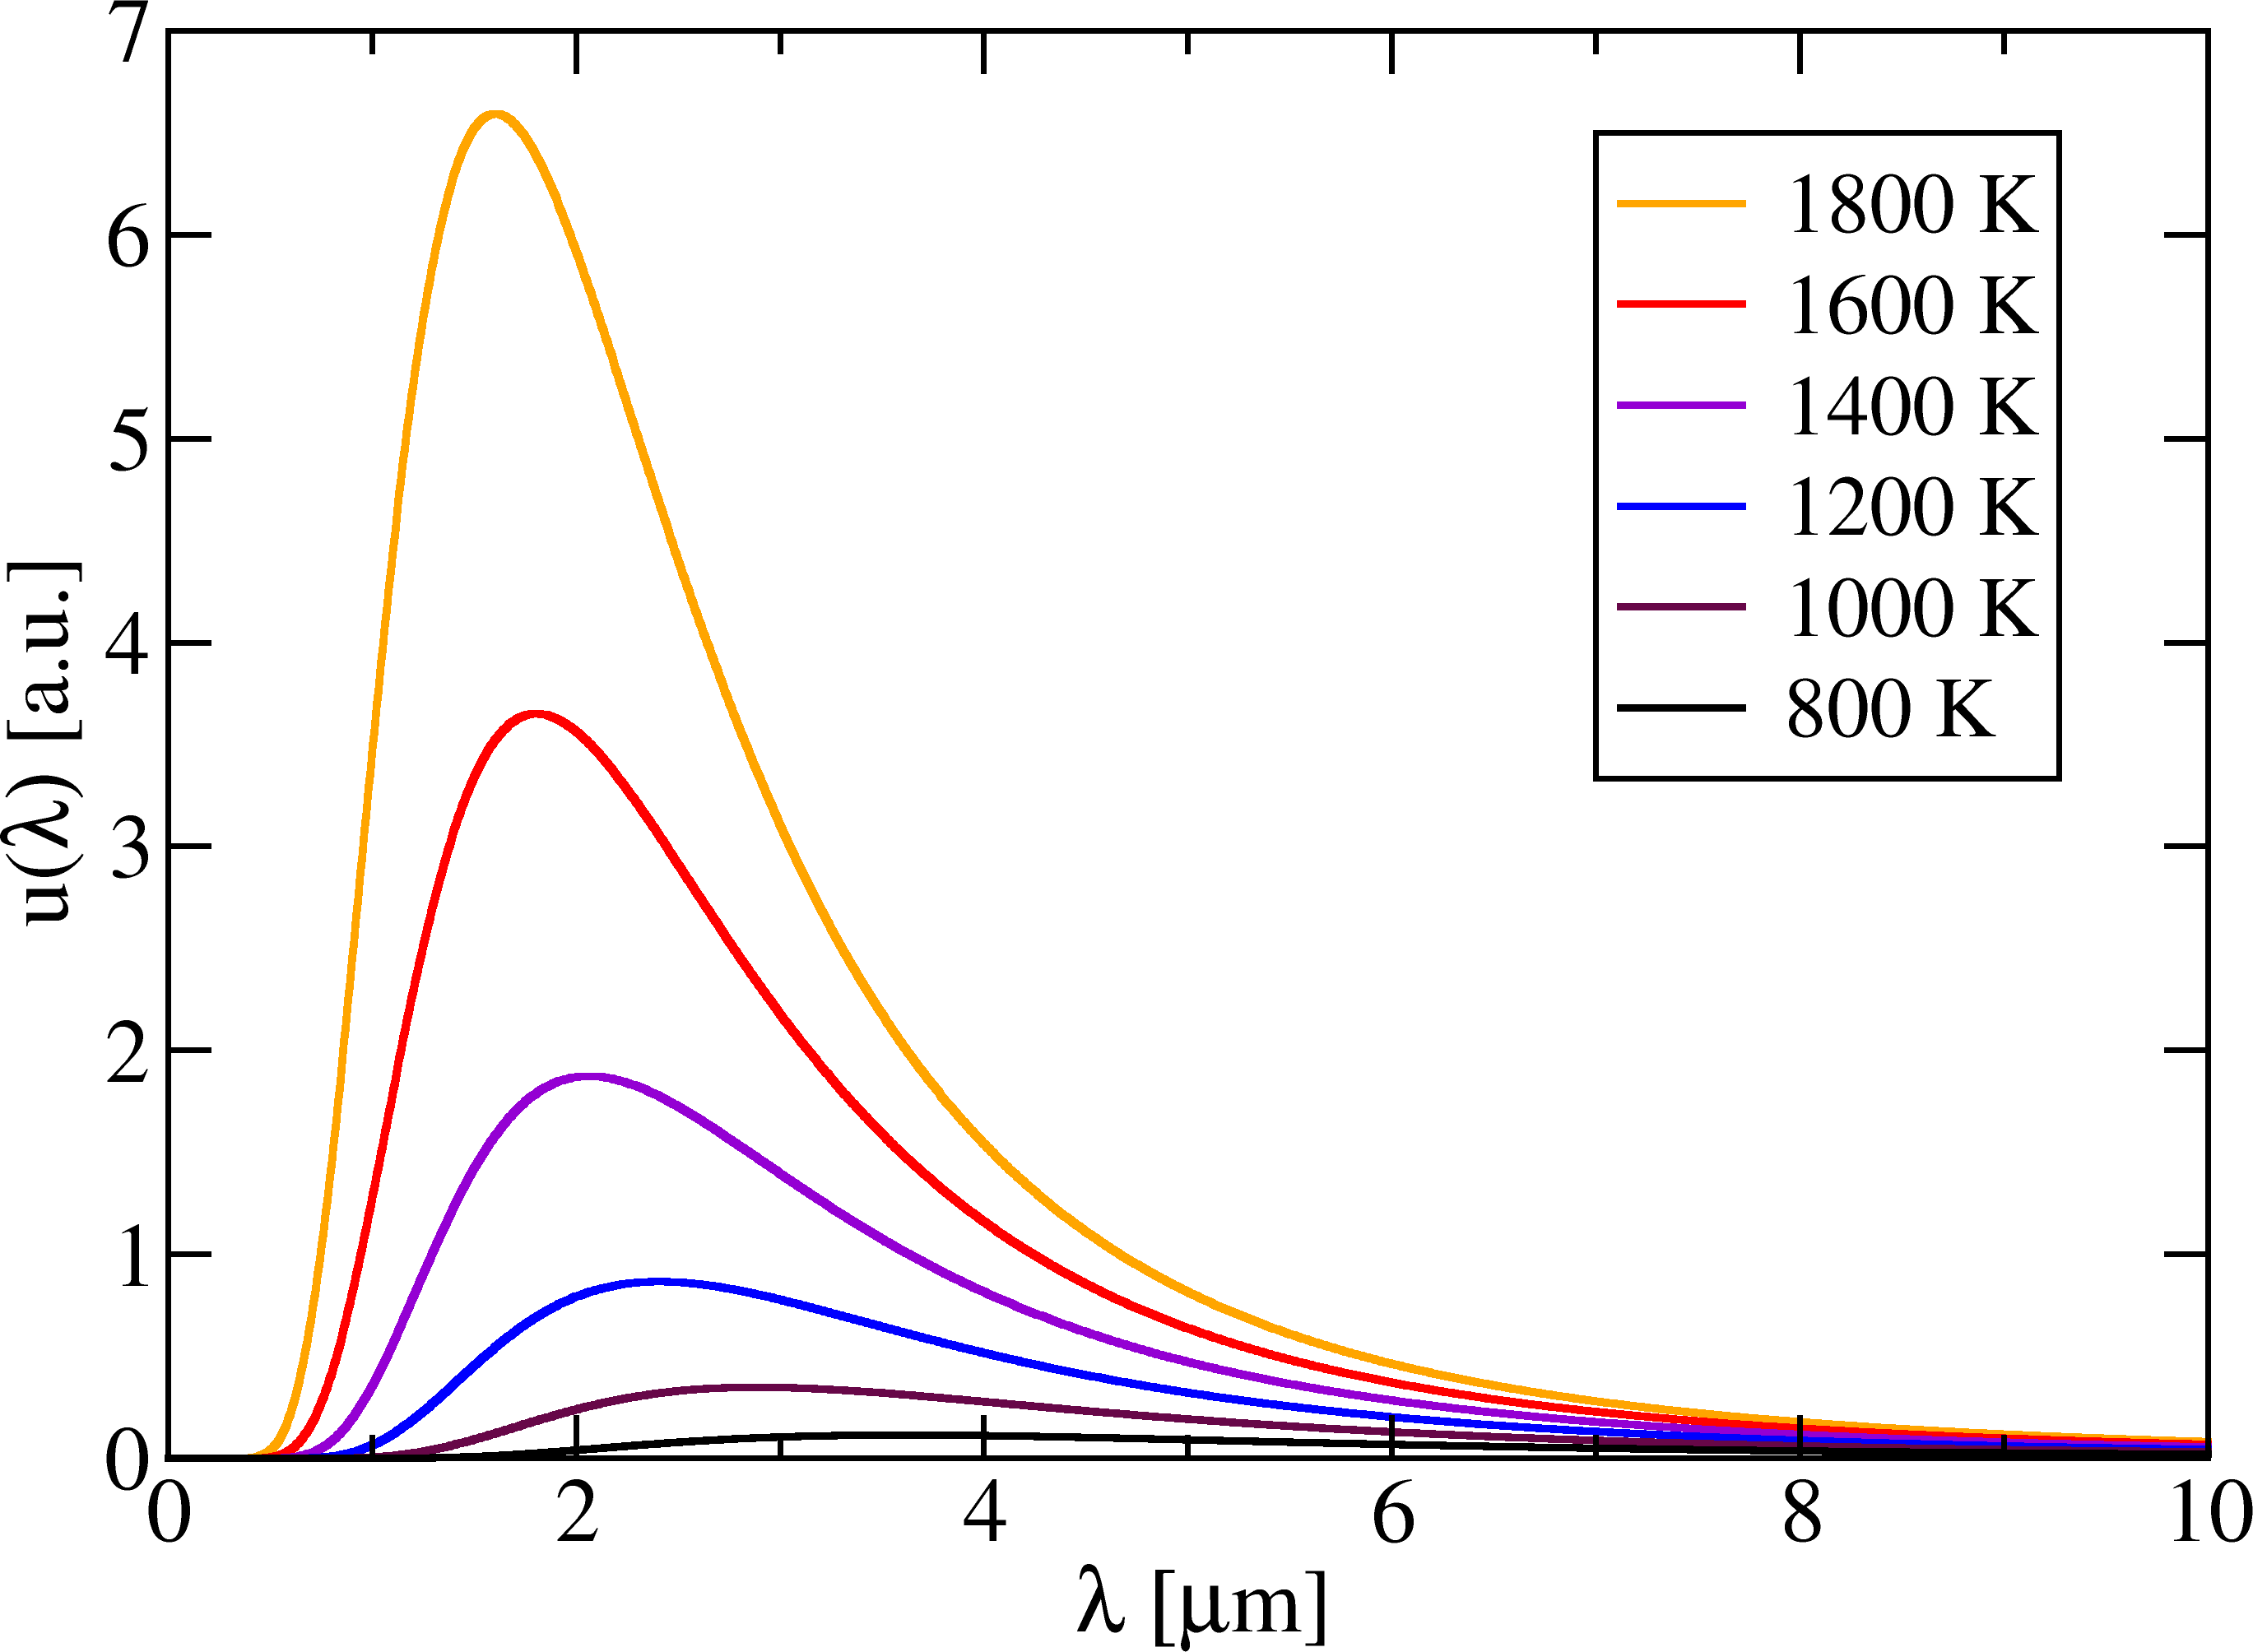
\includegraphics[width=7truecm]{slike/05_Planck.png}
\caption{Planckov spekter za sevanje črnega telesa pri različnih temperaturah}
\label{fig:Planck}
\end{figure}


\section{Absorpcija, spontano in stimulirano sevanje}

Oglejmo si zdaj osnovne procese interakcije svetlobe s snovjo. Naj
bo v votlini poleg elektromagnetnega polja še $N$ atomov, ki se med
seboj ne motijo. Za začetek naj bodo prav enostavni\index{Dvonivojski sistem}: 
imajo naj le dve energijski stanji z energijama $E_{1}$ in $E_{2}>E_1$ (glej sliko~\ref{sl4.1}\,a).\\
\begin{figure}[h]
\centering
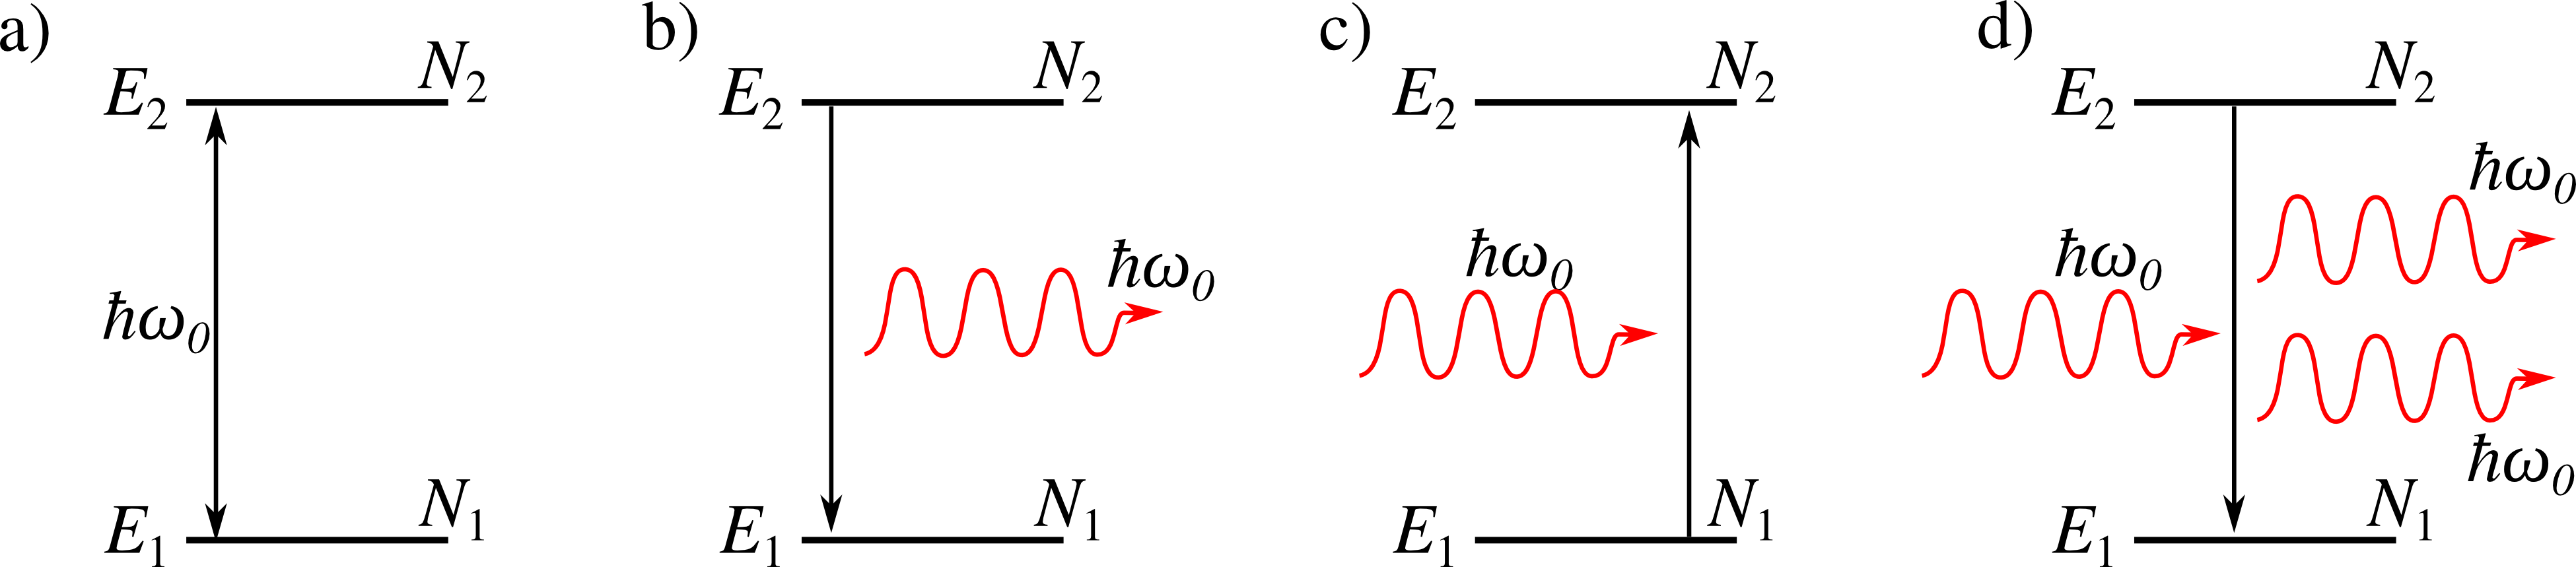
\includegraphics[width=14truecm]{slike/05_Dvonivojski.png}
\caption{Shema energijskih nivojev dvonivojskega atoma (a) in prehodov med njima:
spontano sevanje (a), absorpcija (b) in stimulirano sevanje (c).}
\label{sl4.1}
\end{figure}


Zaradi interakcije s poljem pri frekvenci prehoda $\omega_{0}=(E_{2}-E_{1})/\hbar$
atomi prehajajo iz nižjega stanja v višje in obratno. Trije procesi opisujejo to 
prehajanje: spontano sevanje, absorpcija in stimulirano sevanje. Oglejmo si te procese
bolj natančno.

\subsection*{Spontano sevanje}
Vemo, da atom v vzbujenem stanju tudi brez vpliva zunanjega polja
ni stabilen, temveč prej ali slej preide v nižje stanje. Temu pojavu
pravimo spontano sevanje\index{Spontano sevanje} ali spontana emisija (slika~\ref{sl4.1}\,b). 
Pri spontanem sevanju se izseva foton v katerokoli stanje polja v bližini 
frekvence prehoda. Verjetnost za prehod na enoto časa označimo z $A_{21}$.
Karakteristični razpadni čas gornjega stanja je tako
$1/A_{21}$.

\subsection*{Absorpcija}
Absorpcija fotona\index{Absorpcija fotona} je prehod, pri katerem se foton 
z ustrezno energijo absorbira, atom pa preide iz spodnjega stanja v zgornje (slika~\ref{sl4.1}\,c). 
Verjetnost za prehod na časovno enoto $r_{12}$ je sorazmerna spektralni gostoti
energije polja $u(\omega)$, to je energiji na enoto volumna in frekvenčni interval, 
pri frekvenci prehoda $\omega_{0}$
\begin{equation}
r_{12}=B_{12}u(\omega_{0}).
\label{4.16}
\end{equation}
Vpeljali smo sorazmernostni koeficient $B_{12}$. Pri absorpciji se
seveda zmanjša število fotonov v enem od stanj polja pri frekvenci
$\omega_{0}$.

\subsection*{Stimulirano sevanje}
Tretji pojav je prehod atoma iz gornjega stanja v spodnje zaradi interakcije
s poljem. Temu procesu pravimo stimulirano sevanje\index{Stimulirano sevanje} ali 
stimulirana emisija. Tudi verjetnost za stimuliran prehod na časovno enoto $r_{21}$ 
je sorazmerna spektralni gostoti energije polja pri frekvenci prehoda $\omega_{0}$
\begin{equation}
r_{21}=B_{21}u(\omega_{0}).
\label{4.17}
\end{equation}
V tem primeru smo sorazmernostni koeficient označili z $B_{21}$. V primeru
stimuliranega sevanja, se število fotonov v stanju, ki je prehod povzročilo, poveča za ena. 


Preden nadaljujemo, se še nekoliko pomudimo pri izrazih za absorpcijo
(enačba~\ref{4.16}) in stimulirano emisijo (enačba~\ref{4.17}).
Zaradi končnega življenjskega časa ima gornje
stanje tudi končno spektralno širino. Zapisani enačbi~(\ref{4.16}) in (\ref{4.17})
veljata le, kadar je spektralna gostota elektromagnetnega polja $u(\omega)$
preko celotne širine prehoda približno konstantna (slika~\ref{fig:spektri}\,a). To je gotovo res, če
obravnavamo sevanje v votlini, ki je v termičnem ravnovesju (črno telo). 


Če pa na atome svetimo s svetlobo s spektrom, ki je ozek v primerjavi s širino prehoda, na
primer iz laserskega resonatorja, je verjetnost za prehod odvisna tudi od tega, kako
blizu centralne frekvence prehoda je frekvenca vpadne svetlobe (slika~\ref{fig:spektri}\,b). 
Naj bo $w_{\omega R}$ gostota energije (ne spekter!) monokromatske svetlobe s frekvenco
$\omega_R$. Tedaj lahko verjetnost za absorpcijo na časovno enoto zapišemo
v obliki 
\begin{equation}
r_{12}=B_{12}g(\omega_R)\, w_{\omega R}.
\label{4.18}
\end{equation}
Pri tem funkcija $g(\omega)$ opisuje obliko atomske spektralne črte z vrhom 
pri $\omega_{0}$ ima vrh. \\
\begin{figure}[h]
\centering
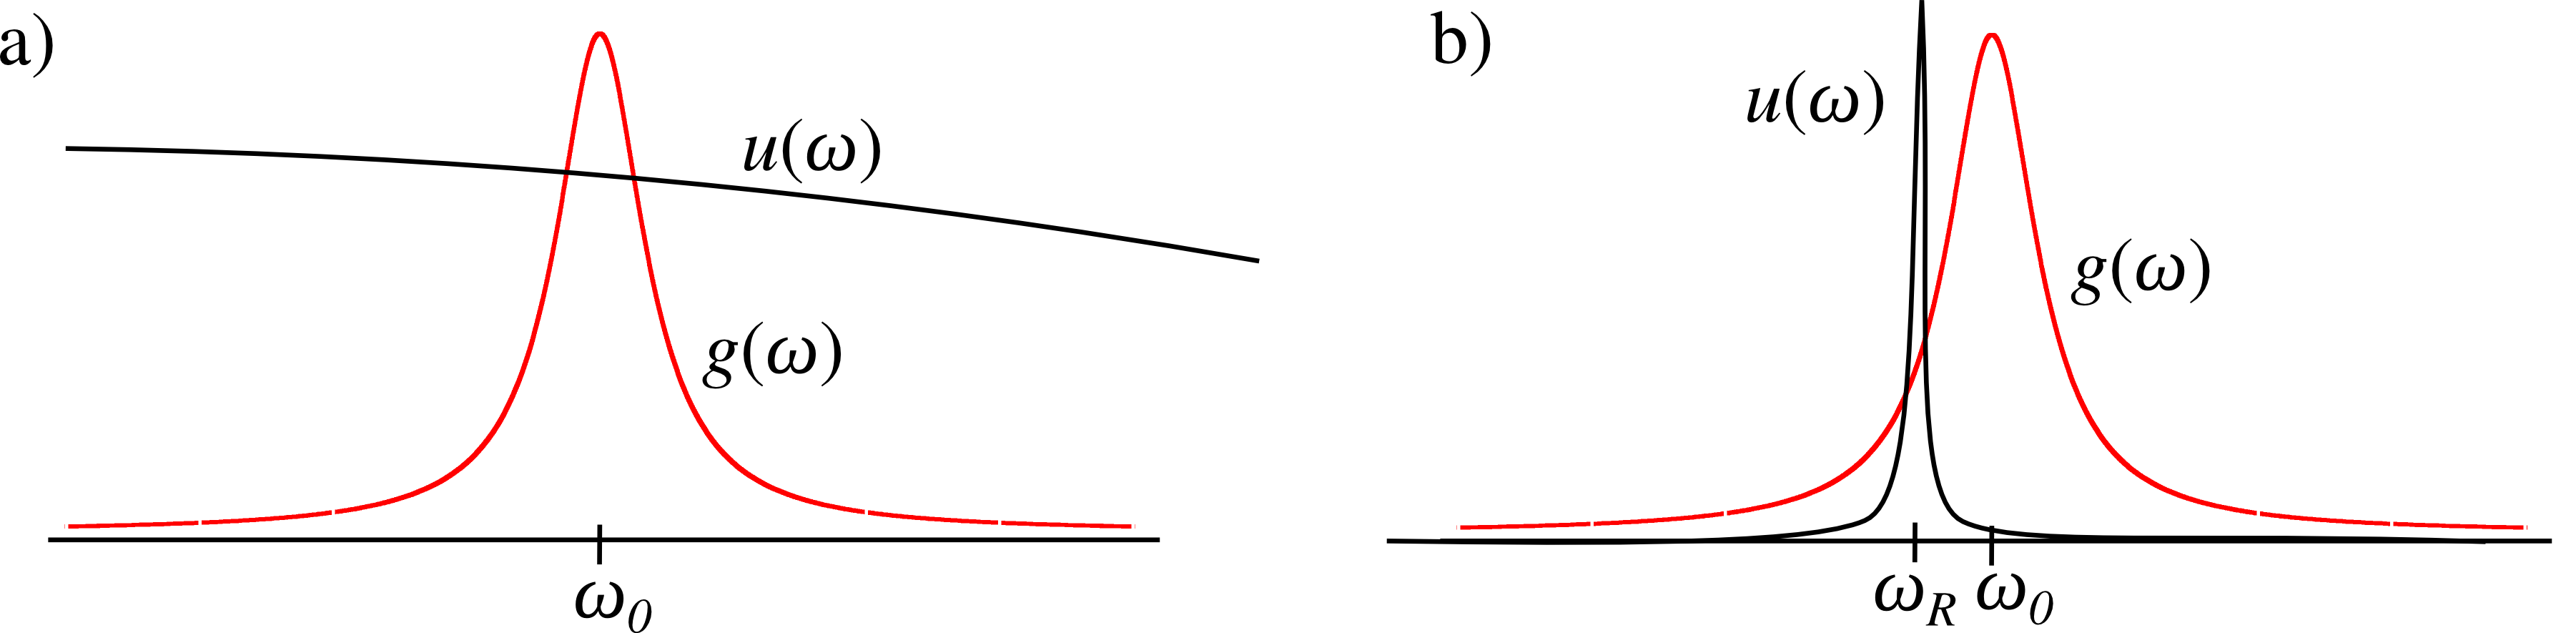
\includegraphics[width=12truecm]{slike/05_Spektri.png}
\caption{Pri izračunu verjetnosti za absorpcijo in stimulirano emisijo je pomembno, ali je 
širina spektralne gostote elektromagnetnega polja bistveno večja (a) ali bistveno manjša (b)
glede na atomsko spektralno črto.}
\label{fig:spektri}
\end{figure}


V splošnem primeru, ko se spekter vpadne svetlobe spreminja v območju 
frekvence prehoda, moramo sešteti prispevke pri posameznih frekvencah (\ref{4.18}) 
po ozkih frekvenčnih intervalih
\begin{equation}
r_{12}=B_{12}\int g(\omega)\, u(\omega)\, d\omega.
\label{4.19}
\end{equation}
Če preverimo gornji zapis na primeru spektra črnega telesa, ki se ne spreminja 
dosti v območju prehoda, lahko $u(\omega)$ postavimo pred integral in po pričakovanju
dobimo znano enačbo~(\ref{4.16}). Iz tega sledi, da mora biti funkcija $g(\omega)$ normirana
\begin{equation}
\int g(\omega)\, d\omega=1.
\label{4.20}
\end{equation}
Zelo pogosto je $g(\omega)$ Lorentzove oblike\index{Lorentzov spekter}
\begin{equation}
g(\omega)=\frac{1}{\pi}\frac{\gamma}{(\omega-\omega_{0})^{2}+\gamma^{2}}.
\label{4.21}
\end{equation}
Za grobe ocene lahko funkcijo $g(\omega)$ aproksimiramo tudi s pravokotnikom širine
$\delta\omega\simeq\gamma$ in višine $1/\delta\omega$.

\subsection*{Einsteinovi koeficienti}
\label{AB}
Vrnimo se k fenomenološkim koeficientom $A_{21}$, $B_{21}$ in $B_{12}$, ki jih je 
vpeljal Einstein\footnote{Nemški fizik in nobelovec Albert Einstein, 1879--1955.}. 
S temi koeficienti, pravimo jim tudi Einsteinovi koeficienti\index{Einsteinovi koeficienti}, 
je mogoče uspešno opisati velik del pojavov pri interakciji svetlobe s snovjo.


Vpeljimo pojem zasedenost stanj\index{Zasedenost stanj}, ki pove število 
atomov v določenem stanju. Ker obravnavamo preproste modele atomov z zgolj 
dvema stanjema, zapišemo samo dve zasedenosti. Naj bo $N_1$ zasedenost 
spodnjega stanja, $N_{2}$ zasedenost zgornjega, skupno število atomov pa
$N=N_1+N_2$. V prisotnosti svetlobe 
se bo število atomov v spodnjem in zgornjem stanju v splošnem spreminjalo, skupno 
število pa se bo ohranjalo.


Obravnavajmo termično ravnovesje, ko je spekter svetlobe bistveno širši
od širine atomskega prehoda (slika~\ref{fig:spektri}\,a), tako da lahko
uporabljamo enačbi~(\ref{4.16}) in (\ref{4.17}). Zasedenost zgornjega nivoja
se zmanjšuje zaradi spontanih in stimuliranih prehodov v spodnje
stanje, povečuje pa se zaradi absorpcije s spodnjega stanja. To zapišemo z enačbo
\begin{equation}
\frac{dN_{2}}{dt}=-A_{21}N_2 - r_{21}N_2 + r_{12}N_1 = 
-A_{21}N_{2}-B_{21}u(\omega_{0})N_{2}+B_{12}u(\omega_{0})N_{1}.
\label{4.22}
\end{equation}
Zaradi ohranitve skupnega števila atomov velja 
\beq
\frac{dN_{1}}{dt}=\frac{-dN_{2}}{dt}.
\eeq
V termičnem ravnovesju sta zasedenosti konstantni, tako da lahko zapišemo 
\begin{equation}
\frac{dN_{1}}{dt}=A_{21}N_{2}+B_{21}u(\omega_{0})N_{2}-B_{12}u(\omega_{0})N_{1}=0.
\label{4.23}
\end{equation}
Vemo pa, da mora biti v termičnem ravnovesju spektralna gostota energije sevanja
$u(\omega)$ kar termična Planckova gostota $u_{T}(\omega)$.
Izrazimo najprej spektralno gostoto iz enačbe~(\ref{4.23})
\begin{equation}
u_{T}(\omega_{0})=\frac{A_{21}}{B_{12}\frac{N_{1}}{N_{2}}-B_{21}}.
\label{4.24}
\end{equation}
Vemo tudi, da v termičnem ravnovesju za zasedenosti $N_{1}$ in $N_{2}$ velja
kanonična porazdelitev
\begin{equation}
\frac{N_{2}}{N_{1}}=e^{-\beta(E_{2}-E_{1})} = e^{-\beta \hbar \omega_0},
\label{4.25}
\end{equation}
kjer je $\beta=1/k_BT$. Sledi
\begin{equation}
u_{T}(\omega_{0})=\frac{A_{21}/B_{12}}{e^{\beta\hbar\omega_{0}}-B_{21}/B_{12}}.
\label{4.26}
\end{equation}
Za določitev koeficientov primerjamo gornji izraz s Planckovo formulo za $u_{T}(\omega_{0})$
(enačba~\ref{eq:Planck}). Očitno morata biti koeficienta $B_{21}$ in $B_{12}$ enaka 
(če sta stanji nedegenerirani), med $A_{21}$ in $B_{12}$ pa velja zveza 
\boxeq{4.27}{
A_{21}=\frac{\hbar\omega^{3}}{\pi^{2}c^{3}}\, B_{12} \qquad \mathrm{in} \qquad B_{12}=B_{21}.
}
Koeficient pred $B_{12}$ je ravno enak gostoti stanj elektromagnetnega polja 
$\rho(\omega)$ (enačba~\ref{4.4}), pomnoženi z energijo fotona $\hbar\omega$. 
Videli bomo, da to ni slučajno in da sledi iz verjetnosti za prehod v kvantni 
elektrodinamiki (poglavje~\ref{chap:verjetnost}).
Pozoren bralec je lahko tudi opazil, da je z enačbo~(\ref{4.26}),
ki smo jo dobili le z uporabo kanonične porazdelitve za atome, že
določena oblika Planckove formule, ne da bi karkoli rekli o fotonih.

\section{Absorpcijski koeficient}

V prejšnjem razdelku smo napovedali, da lahko velik del pojavov pri interakciji 
svetlobe s snovjo opišemo z Einsteinovimi koeficienti. Poskusimo zdaj 
koeficienta $A_{21}$ in $B_{21}$ povezati z makroskopskim absorpcijskim
koeficientom plina atomov. 


Naj na izbran volumen plina vpada snop svetlobe s frekvenco
$\omega$, ki je blizu frekvence atomskega prehoda $\omega_{0}$. Gostota
vpadnega energijskega toka je $j_{\omega}=w_{\omega}c$ (enačba~\ref{eq:jcw}), 
pri čemer je $w_{\omega}$ gostota energije. Obravnavajmo primer, ko je 
spekter vpadnega snopa ozek v primerjavi s širino atomskega prehoda
(slika~\ref{fig:spektri}\,b). V tej obliki zapisane enačbe bodo bolj 
priročne pozneje pri obravnavi laserja. Privzemimo še, da
je stanje stacionarno. 
\begin{figure}[h]
\centering
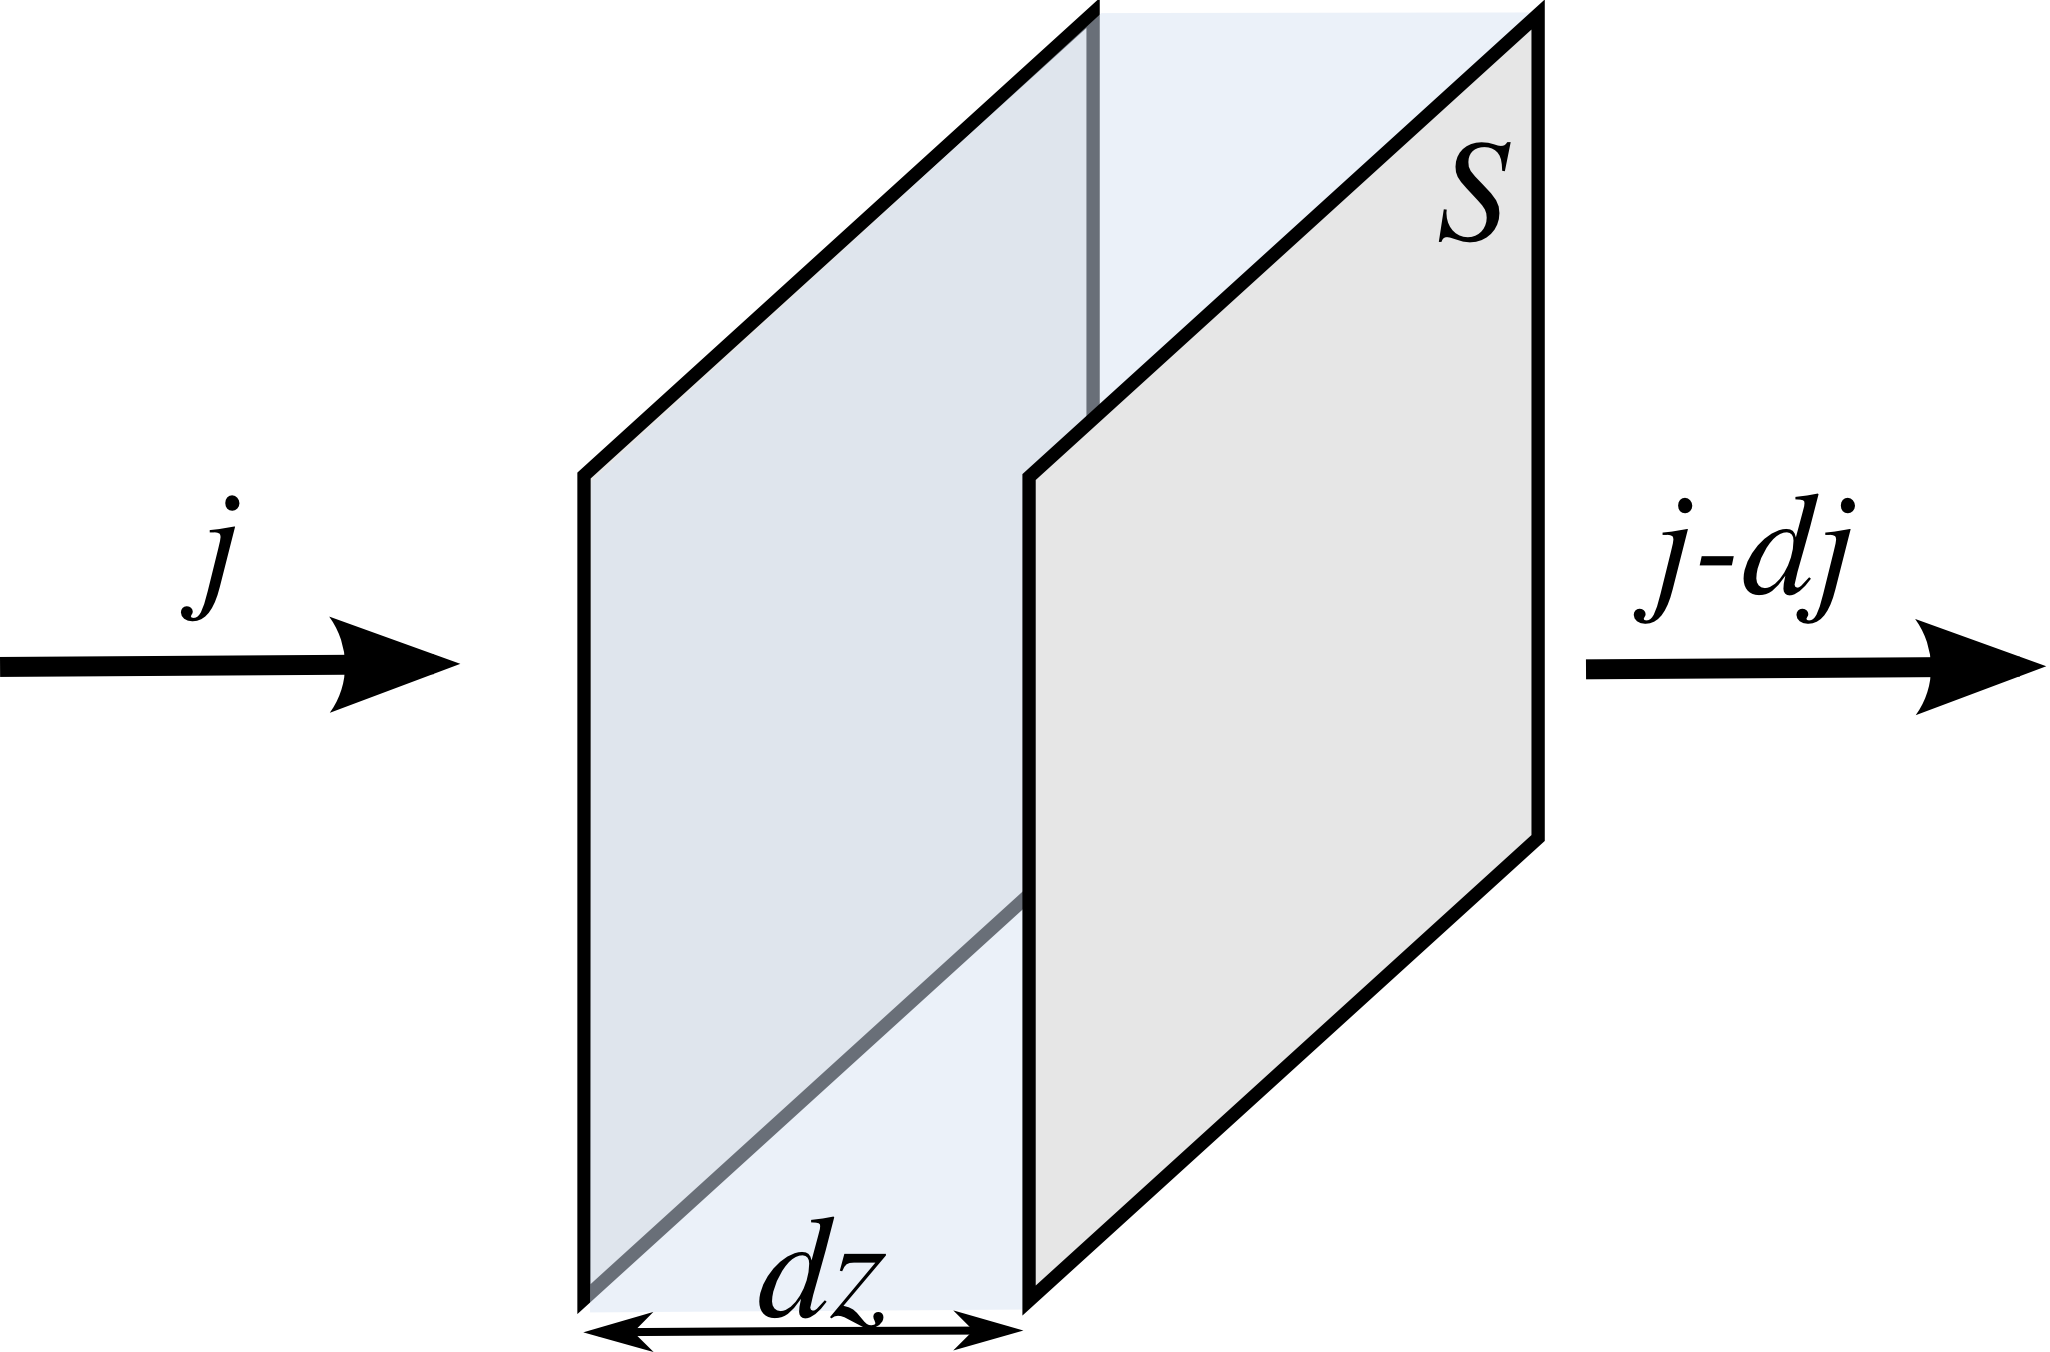
\includegraphics[width=6truecm]{slike/05_Absorpcija.png}
\caption{K absorpciji snopa svetlobe v plasti atomov}
\label{fig:abs}
\end{figure}

 
Ko svetloba vpade na plast plina debeline $dz$, se gostota
energijskega toka zmanjša zaradi absorpcije in hkrati poveča zaradi 
stimulirane emisije (slika~\ref{fig:abs}). 
Spontano sevanje, ki je seveda tudi prisotno, lahko zanemarimo, saj
bo izsevano na vse strani enakomerno in ga bo le zelo majhen del v smeri snopa.
Sprememba energije snopa na enoto časa je enaka razliki med 
številom absorpcij in stimuliranih prehodov na enoto časa, pomnoženih z 
energijo fotona. To popišemo z enačbo 
\begin{equation}
dP=S\, dj=(N_{2}-N_{1}) \, \frac{S dz}{V} \, \hbar\omega \,r_{12} = 
(N_{2}-N_{1})\, \frac{S dz}{V}\, \hbar\omega \, B_{21}g(\omega) w_{\omega},
\label{4.28}
\end{equation}
pri čemer smo verjetnost z prehod izrazili iz enačbe~(\ref{4.18}).
S $S$ smo označili presek snopa, z $V$ pa volumen plina. Tako dobimo 
enačbo za spreminjanje gostote toka 
\begin{equation}
dj=\frac{1}{V}(N_{2}-N_{1})\, B_{21}g(\omega)\, \frac{\hbar\omega}{c}j_{\omega}\, dz
\label{4.29}
\end{equation}
Priročno je vpeljati še presek za absorpcijo\index{Presek za absorpcijo} ali
stimulirano sevanje\index{Presek za stimulirano sevanje} 
\beq
\sigma(\omega)=\frac{B_{21}\, g(\omega)\, \hbar\omega}{c}.
\label{sigma}
\eeq
Z njim se izraz (\ref{4.29}) poenostavi v 
\boxeq{4.30}{
\frac{dj}{dz}=\frac{N_{2}-N_{1}}{V}\sigma(\omega)j.
}
Navadno imamo opravka s plinom, ki je blizu termičnega ravnovesja,
zato je $N_{2}<N_{1}$ in je $dj$ negativen. V tem primeru pride do
absorpcije\index{Absorpcija} z absorpcijskim koeficientom\index{Absorpcijski koeficient}
\begin{equation}
\mu(\omega)=\frac{N_{1}-N_{2}}{V}\, B_{21}\, g(\omega)\frac{\hbar\omega}{c}=
\frac{N_{1}-N_{2}}{V}\sigma(\omega),
\label{4.31}
\end{equation}
za gostoto energijskega toka pa velja enačba
\beq
\frac{dj}{j} = -\mu dz.
\label{eq:jabs}
\eeq
Energija se pri absorpciji na našem plinu dvonivojskih atomov seveda
ne izgublja, temveč le siplje. Atom, ki je prešel v vzbujeno stanje,
se s spontano emisijo vrne nazaj v osnovno, svetloba pa se izseva
na vse strani -- se siplje.

\section{Nasičenje absorpcije}
\label{chap:NasAbs}

Čeprav je na prvi pogled enačba~(\ref{eq:jabs}) za zmanjševanje 
gostote svetlobnega toka pri prehodu skozi absorbirajoči plin preprosta,
je ni mogoče enostavno integrirati, saj je $\mu$ odvisen od 
gostote energijskega toka. Pri dovolj veliki gostoti
svetlobnega toka namreč z absorpcijo znaten delež
atomov preide v višje stanje, zaradi česar se zmanjša razlika $N_{1}-N_{2}$,
posledično se pa zmanjša tudi absorpcijski koeficient -- absorpcija
se nasiti. Zato temu pojavu pravimo nasičenje absorpcije\index{Nasičena absorpcija}.
Obravnavajmo ga še matematično.


Obravnavajmo snop monokromatske svetlobe, ki vpada na plin. 
Atomi v plinu prehajajo med nivoji zaradi absorpcije, spontane in stimulirane emisije. 
Podobno kot smo zapisali enačbo~(\ref{4.23}) za termično ravnovesje v primeru
širokega spektra, zapišemo stacionarno enačbo za naš primer kot
\begin{equation}
A_{21}N_{2}+B_{21}\,g(\omega)\,(N_{2}-N_{1})\frac{j}{c}=0,
\label{4.32}
\end{equation}
pri čemer smo za verjetnost za prehod namesto enačbe~(\ref{4.17}) vzeli
enačbo~(\ref{4.18}). Zasedenost višjega stanja $N_{2}$ lahko izrazimo s 
celotnim številom atomov $N$ in razliko zasedenosti 
\beq
N_{2}=\frac{1}{2}N+\frac{1}{2}(N_{2}-N_{1}).
\label{4.321}
\eeq
S tem lahko izračunamo razliko zasedenosti 
\begin{equation}
N_{2}-N_{1}=-\frac{N}{1+2\frac{Bg(\omega)}{cA}j}.
\label{4.33}
\end{equation}
Pri majhni gostoti toka $j$ so praktično vsi atomi v osnovnem stanju in prispevajo
k absorpciji. Pri velikih gostotah toka pa imenovalec gornjega
izraza močno naraste, razlika zasedenosti gre proti nič in absorpcija se zmanjšuje.
Ko drugi člen v imenovalcu enačbe~(\ref{4.33}) doseže vrednost 1, pravimo, da
gostota energijskega toka doseže vrednost saturacijske gostote\index{Saturacijska gostota toka}.
Zapišemo jo kot 
\begin{equation}
j_{s}(\omega)=\frac{cA_{21}}{2B_{21}g(\omega)}=
\frac{\hbar\omega^{3}}{2\pi^{2}c^{2}g(\omega)},
\label{4.34}
\end{equation}
pri čemer smo upoštevali zvezo~(\ref{4.27}) med koeficientoma $A_{21}$ in $B_{21}$.
Kot vidimo, je saturacijska gostota odvisna le od frekvence vpadnega valovanja 
in širine atomskega prehoda. Za črto z valovno dolžino okoli 600~nm in širino črte
$10^{8}~\mathrm{s}^{-1}$ znaša saturacijska gostota svetlobnega toka okoli 
$20~\mathrm{mW/cm}^{2}$. Tako gostoto toka v ozek frekvenčni interval
je z običajnimi svetili, na primer plinsko razelektritveno cevjo,
praktično nemogoče doseči, medtem ko jo iz laserjev dobimo z lahkoto.
Izraz za razliko zasedenosti stanj lahko zdaj zapišemo v pregledni obliki
\begin{equation}
N_{2}-N_{1}=-\frac{N}{1+\frac{j}{j_{s}(\omega)}}.
\label{4.35}
\end{equation}
Vstavimo gornji izraz v enačbo za zmanjševanje gostote toka (enačba~\ref{4.30}) in 
dobimo 
\boxeq{4.36}{
dj=-\frac{\mu_{0}}{1+\frac{j}{j_{s}}}\, j\, dz,
}
kjer smo z $\mu_{0}=N\,B_{21}\,g(\omega)\,\hbar\omega/Vc$ označili
absorpcijski koeficient pri majhnih gostotah vpadnega toka.
Enačbo brez težav integriramo in dobimo 
\begin{equation}
\ln\frac{j}{j_{0}}+\frac{1}{j_{s}}(j-j_{0})=-\mu_{0}\, z,\label{4.37}
\end{equation}
kjer smo z $j_{0}$ označili začetno gostoto toka. 
\begin{figure}[h]
\centering
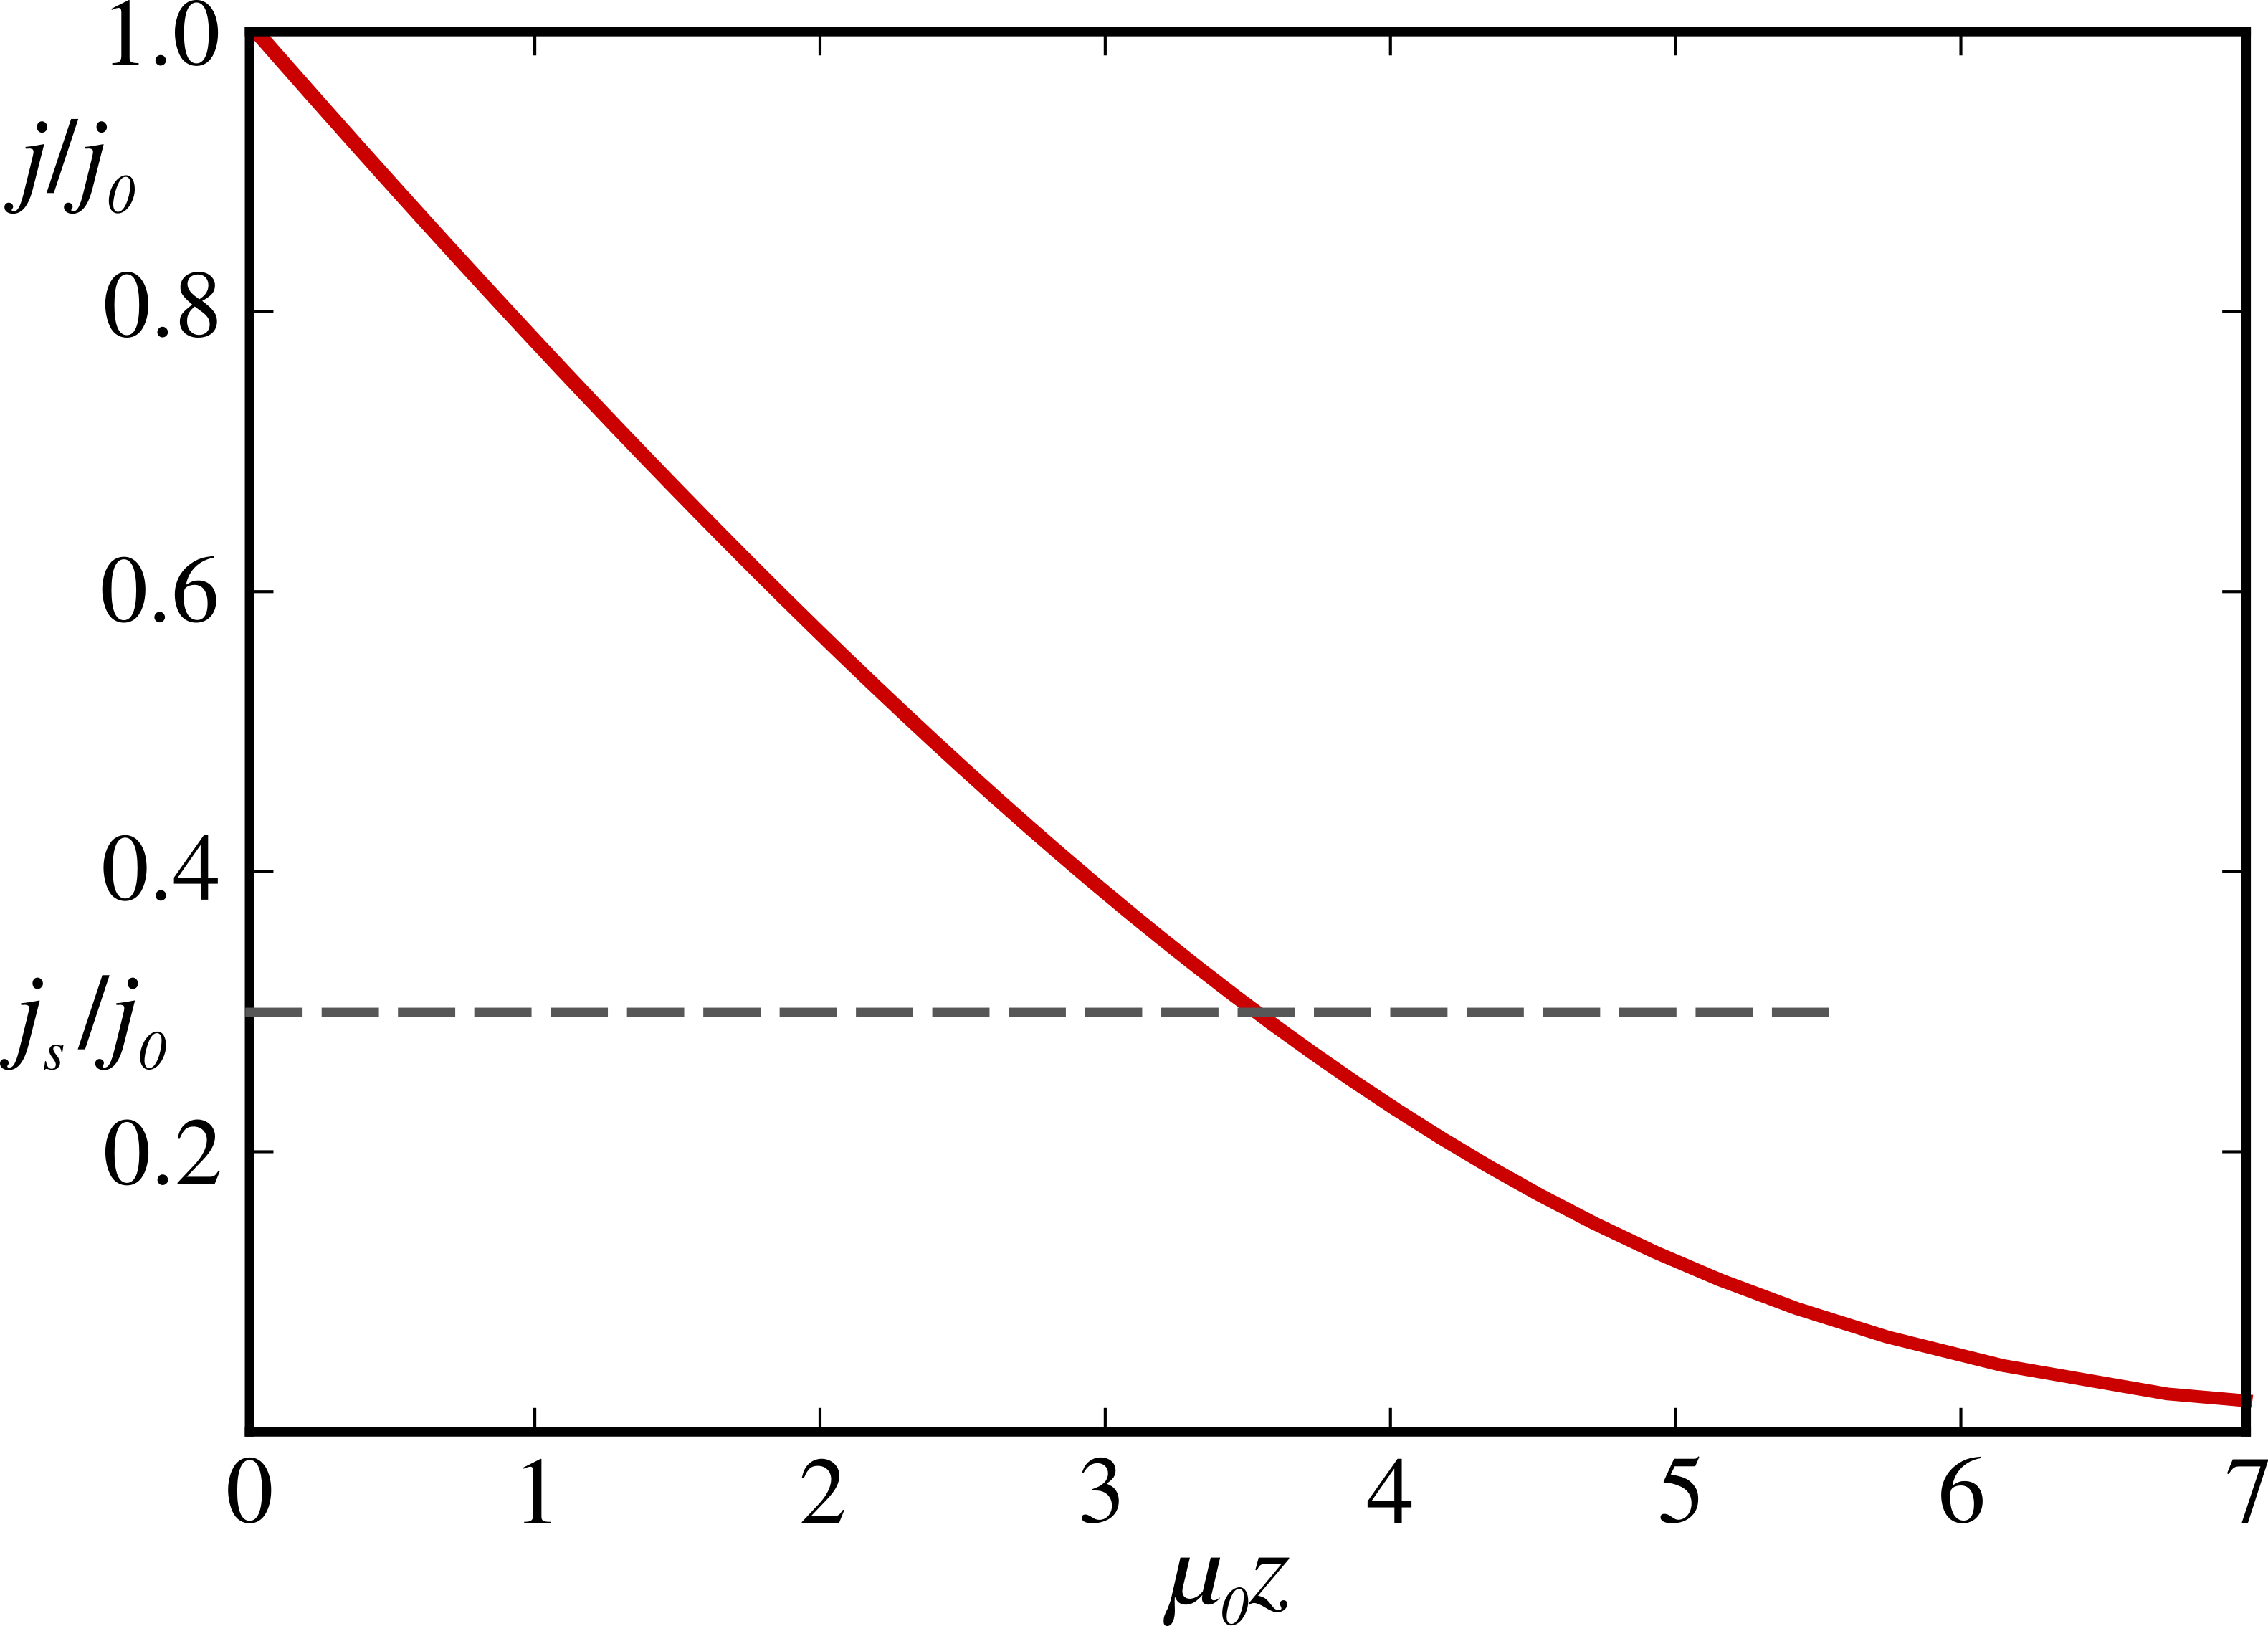
\includegraphics[width=8truecm]{slike/05_jabs.png}
\caption{Pojemanje gostote svetlobnega toka v absorbirajočem plinu}
\label{fig:abs}
\end{figure}
Kadar je ta dosti
manjša od $j_{s}$, lahko drugi člen v gornji enačbi zanemarimo in dobimo 
navadno eksponentno pojemanje
\beq
j = j_0 e^{-\mu_0 z}.
\eeq
Pri zelo velikih vpadnih gostotah pa lahko zanemarimo prvi člen in dobimo, 
da je pojemanje zgolj linearno
\begin{equation}
j=j_{0}-\mu_{0}j_{s}z=j_{0}-\frac{N}{2V}A\hbar\omega\, z.
\label{4.38}
\end{equation}
V primeru močnega vpadnega toka je zasedenost spodnjega in zgornjega nivoja skoraj
enaka in je absorpcija omejena s tem, kako hitro se atomi vračajo
v osnovno stanje preko spontanega sevanja, kar je razvidno tudi iz
zadnje oblike izraza~(\ref{4.38}).

\section{Optično ojačevanje}
V prejšnjih razdelkih smo obravnavali prehod svetlobe skozi dvonivojski plin. V primeru
termičnega ravnovesja je zgornji nivo manj zaseden od spodnjega in v plinu pride
do absorpcije svetlobe. Če pa nekako dosežemo primer, da je $N_{2}>N_{1}$, 
se bo snop svetlobe pri prehodu skozi tako pripravljen plin ojačeval. 
Takemu primeru pravimo stanje obrnjene zasedenosti\index{Obrnjena zasedenost}. 
Tako stanje seveda ni v termičnem ravnovesju in ga je treba vzdrževati z dovajanjem 
energije plinu. Dovajanju energije pravimo tudi optično črpanje\index{Optično črpanje}. 
Načinov, kako dosežemo obrnjeno zasedenost z optičnim črpanjem je veliko. Oglejmo 
si nekaj primerov. 


V plinih je najpogostejši način vzbujanja z električnim tokom. Elektroni,
ki so glavni nosilci toka, se zaletavajo v atome ali ione in jih vzbujajo
na višje nivoje, pri čemer lahko pride do obrnjene zasedenosti med
nekim parom nivojev. Pogost proces v plinih je tudi prenos energije
med atomi s trki. Vzemimo mešanico dveh plinov, pri katerih se nek
nivo enih atomov ujema po energiji s stanjem drugih atomov. Vzbujen
atom prve vrste lahko pri trku preda energijo brez sevanja atomu druge
vrste, ki iz osnovnega stanja preide v ustrezen višji nivo. Če je
pod tem nivojem še drugo vzbujeno stanje, bomo med njima dobili obrnjeno
zasedenost, kadar je življenjski čas gornjega nivoja daljši od spodnjega.


V trdnih neprevodnih kristalih sta v optičnem področju absorpcija
in sevanje pri določeni valovni dolžini navadno posledica primesi.
Obrnjeno zasedenost para nivojev primesi največkrat dobimo tako, da
kristal obsevamo s svetlobo s frekvenco, ki ustreza prehodu na nek
nivo nad izbranim parom. Tak način optičnega črpanja deluje tudi v
organskih barvilih.


V polprevodnikih dosežemo obrnjeno zasedenost med prevodnim in valenčnim
pasom z vbrizgavanjem elektronov in vrzeli v območje p-n spoja z električnim
tokom v prevodni smeri. Možen mehanizem vzbujanja so tudi kemične
reakcije. Po reakciji lahko produkti ostanejo v vzbujenem stanju
in lahko dobimo obrnjeno zasedenost med paroma stanj.


Nekoliko bolj podrobno si bomo nekaj teh mehanizmov ogledali v nadaljevanju
na konkretnih laserjih. Zaenkrat si kot primer oglejmo le model optičnega
črpanja plina atomov s tremi stanji.


\section{Optično črpanje trinivojskega sistema}

Naj imajo atomi poleg osnovnega stanja z energijo $E_0$, označimo ga $|0\rangle$,
še dve vzbujeni stanji z energijo $E_1$ (stanje $|1\rangle$) in energijo $E_2>E_1$
(stanje $|2\rangle$). Na plin svetimo s svetlobo, ki
vzbuja atome iz stanja $|0\rangle$ v stanje $|2\rangle$, pri čemer
je lahko spektralna gostota $u_{p}$ črpalne svetlobe široka. Poleg
tega naj se po plinu širi še monokromatska svetloba s frekvenco $\omega$
blizu frekvence prehoda $\omega_{0}$ med stanjema $|1\rangle$ in
$|2\rangle$ in z gostoto energije $w$. Ugotoviti želimo, pri kakšnih
pogojih lahko dosežemo obrnjeno zasedenost med stanjema $|1\rangle$ in $|2\rangle$
in s tem ojačevanje svetlobe okoli frekvence $\omega_{0}$.
\begin{figure}[h]
\centering
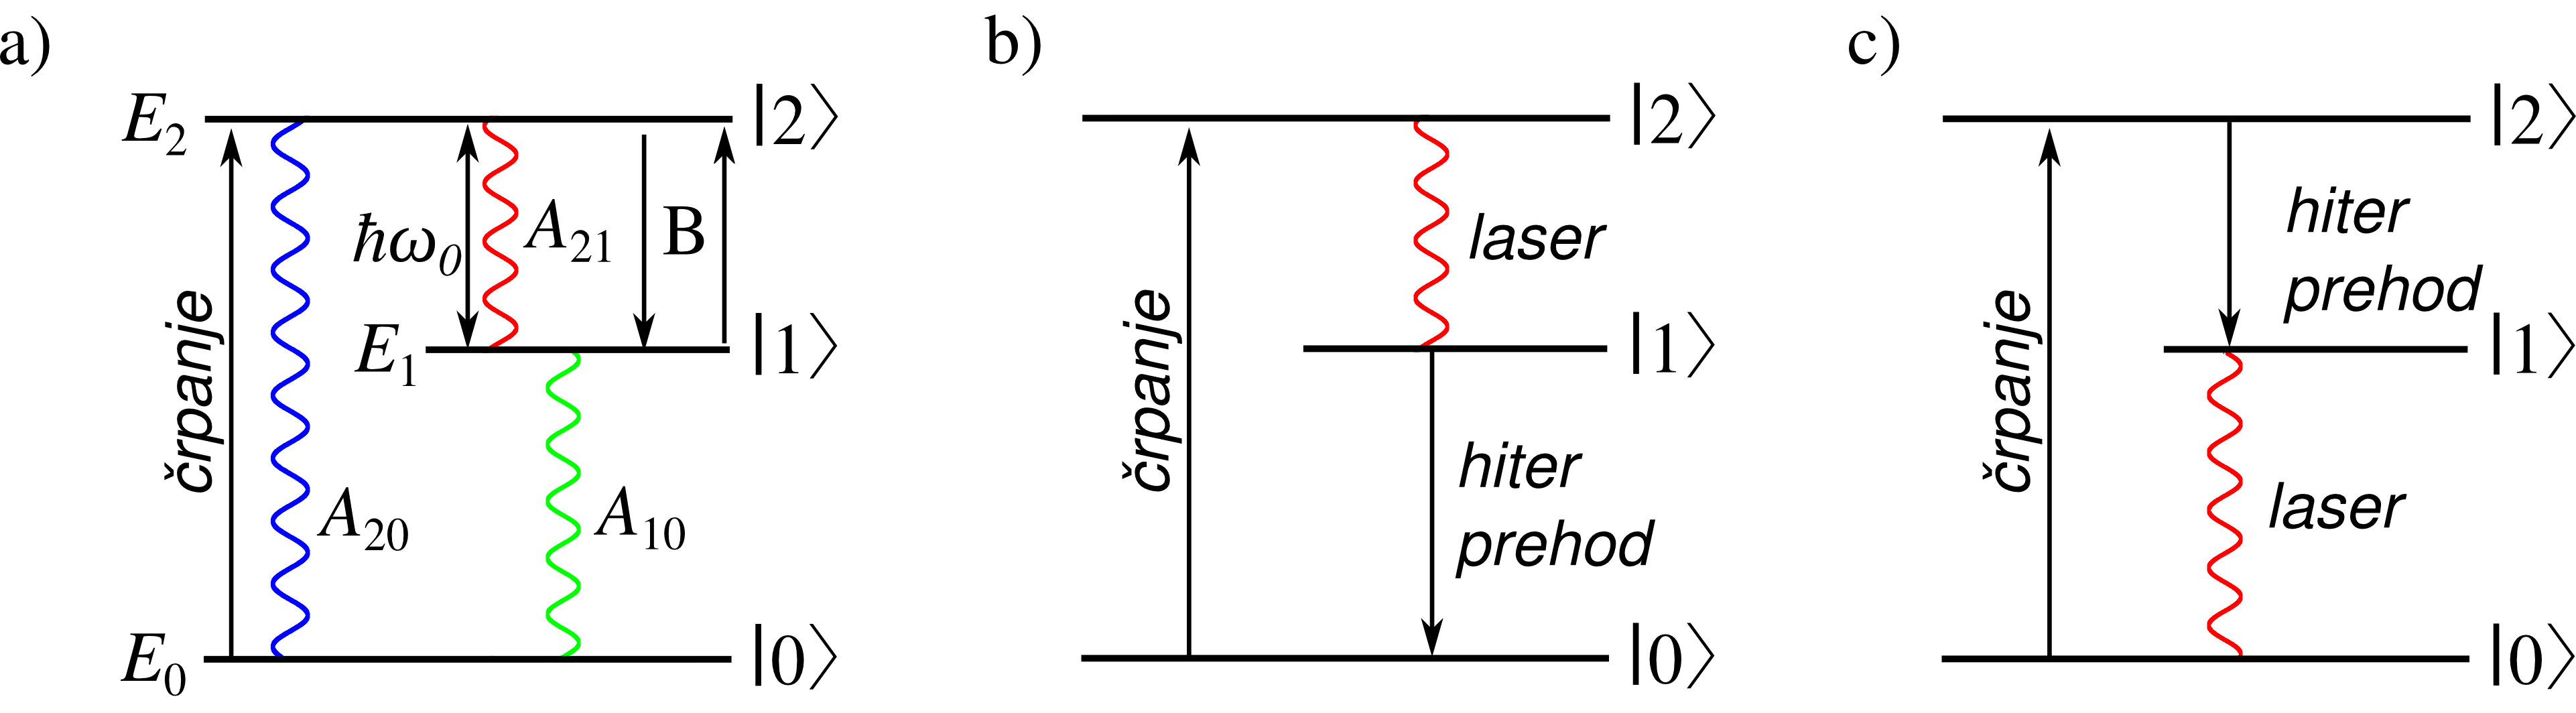
\includegraphics[width=14truecm]{slike/05_Trinivojski.png}
\caption{Shema energijskih nivojev trinivojskega sistema in prehodov med njimi (a).
V plinskih laserjih imamo navadno stanje obrnjene zasedenosti med drugim in prvim
vzbujenim stanjem (b), v navadni trdninskih laserjih (npr. rubinskem) pa med 
prvim vzbujenim in osnovnim stanjem (c).}
\label{fig:3nivojski}
\end{figure}


Zapišimo enačbe za spreminjanje zasedenosti posameznih stanj. Osnovno stanje
se prazni zaradi absorpcije črpalne svetlobe in polni zaradi
spontanih prehodov iz stanj $|1\rangle$ in $|2\rangle$, stimulirane
prehode iz stanja $|2\rangle$ pa bomo zanemarili. Zasedenost stanja $|2\rangle$ se
povečuje zaradi absorpcije s spodnjih nivojev in zmanjšuje
zaradi spontanega in stimuliranega sevanja. Srednje stanje se polni
s stimuliranimi in spontanimi prehodi iz stanja $|2\rangle$ in prazni
zaradi absorpcije v $|2\rangle$ in spontanih prehodov v $|0\rangle$.
Pri tem velja, da je vsota vseh treh zasedenosti enaka številu vseh atomov: $N_{0}+N_{1}+N_{2}=N$. 
Zasedbene enačbe so torej 
\begin{eqnarray}
\frac{dN_{0}}{dt} & = & -rN+A_{20}N_{2}+A_{10}N_{1} \label{4.39.1}\\
\frac{dN_{1}}{dt} & = & -A_{10}N_{1}+B_{21}\,g(\omega)\,w\, (N_{2}-N_{1})+A_{21}N_{2} \label{4.39.2}\\
\frac{dN_{2}}{dt} & = & rN_0-A_{20}N_{2}-A_{21}N_{2}+B_{21}\,g(\omega)\,w\, (N_1-N_2),
\label{4.39}
\end{eqnarray}
pri čemer predpostavili, da je $N_0 \approx N \gg N_1, N_2$ in zato lahko črpanje $B_{20}\, 
u_{p} (N_0-N_2)$, ki je praktično konstantno, zapisali s koeficientom $r$. Mehanizem črpanja 
smo tako skrili v $r$ in prav nič ni pomembno, na kakšen način poteka. 


Zanima nas stacionarno stanje, ko so vsi trije časovni odvodi enaki nič. 
Brez škode lahko tudi zanemarimo spontano sevanje iz stanja
$|2\rangle$ v osnovno stanje. Tako iz druge enačbe sistema~(\ref{4.39.2}) 
dobimo
\begin{eqnarray}
B_{21}\,g(\omega\,)w\, N_{2}+A_{21}N_{2} = B_{21}\,g(\omega\,)w\, N_{1} + A_{10}N_{1} 
\end{eqnarray}
in
\begin{eqnarray}
N_2 = \frac{B_{21}\,g(\omega\,)w + A_{10}}{B_{21}\,g(\omega\,)w+A_{21}}N_1.  
\end{eqnarray}
Ob upoštevanju zveze, ki jo dobimo iz prve enačbe sistema~(\ref{4.39.1})
\beq
N_1= \frac{rN}{A_{10}}, 
\eeq
zapišemo razliko zasedenosti kot 
\begin{equation}
N_{2}-N_{1}=\left(\frac{N_2}{N_1}-1\right)N_1=\frac{A_{10}-A_{21}}{A_{21}+
B_{21}g(\omega)w} \,\frac{rN}{A_{10}}.
\label{4.42}
\end{equation}
Iz gornje enačbe sledi, da dobimo obrnjeno zasedenost, če je $A_{10}>A_{21}$, torej kadar je
razpadni čas stanja $|1\rangle$ krajši kot razpadni čas stanja $|2\rangle$.
Tak rezultat smo seveda lahko pričakovali.


V praktični primerih navadno velja $A_{10}\gg A_{21}$. Ob upoštevanju zveze $j=wc$ povežemo
razliko zasedenosti z gostoto vpadnega svetlobnega toka
\beq
N_{2}-N_{1}=\frac{rN}{A_{21}} \, \frac{1}{1+\frac{B_{21}g(\omega)j}{c A_{21}}} = 
\frac{rN}{A_{21}} \, \frac{1}{1+j/j_s}.
\label{eq:3n_N}
\eeq
Konstante $c A_{21}/B_{21}g(\omega)$ smo pospravili v $j_s$, ki ga bomo imenovali 
saturacijska gostota svetlobnega toka\index{Saturacijska gostota toka}. Vidimo, da je dobljen
izraz zelo podoben saturacijski gostoti za dvonivojski sistem (enačba~\ref{4.34}), razlika je le
v faktorju 2. Do te razlike pride zaradi različnega števila stanj in pogoj $N_{1}+N_{2}=N$
ne velja več. 

\begin{definition}
 Pokaži, da je saturacijska gostota toka $j_2$ odvisna le od frekvence valovanja in širine 
 atomske črte $\delta \omega$. 
\end{definition}



Poglejmo zdaj, kaj se ob vpadu na plast trinivojskega plina zgodi s svetlobo s frekvenco $\omega$ in 
gostoto svetlobnega toka $j=wc$. Račun je zelo podoben računu pri absorpciji (enačba~\ref{4.29}). Zapišemo
spremembo gostote toka na debelini $dz$ 
\begin{equation}
dj=\frac{1}{V}(N_{2}-N_{1})\, B_{21}g(\omega)\, \frac{\hbar\omega}{c}j\, dz,
\label{eq:dj}
\end{equation}
pri čemer gostota toka $j = wc$ nastopa tudi v izrazu za razliko zasedenosti (enačba~\ref{eq:3n_N}). 
Če to upoštevamo, dobimo diferencialno enačbo za gostoto toka
\begin{equation}
\frac{1}{j}\left(1+\frac{j}{j_{s}}\right)\, dj=G\, dz
\label{4.43}
\end{equation}
oziroma
\boxeq{eq:djG}{
dj=\frac{G}{1+\frac{j}{j_{s}}}\, j\, dz,
}
ki je spet zelo podobna enačbi za absorpcijo (enačba~\ref{4.36}).
Z $G$ smo označili t.i. koeficient ojačenja pri majhnih vpadnih gostotah
toka. Podan je z 
\begin{equation}
G=\frac{rNB_{21}\hbar\omega g(\omega)}{VcA_{21}}.\label{4.44}
\end{equation}
Rešitev diferencialne enačbe je prikazana na sliki~(\ref{fig:ojacanje}). 
\begin{figure}[h]
\centering
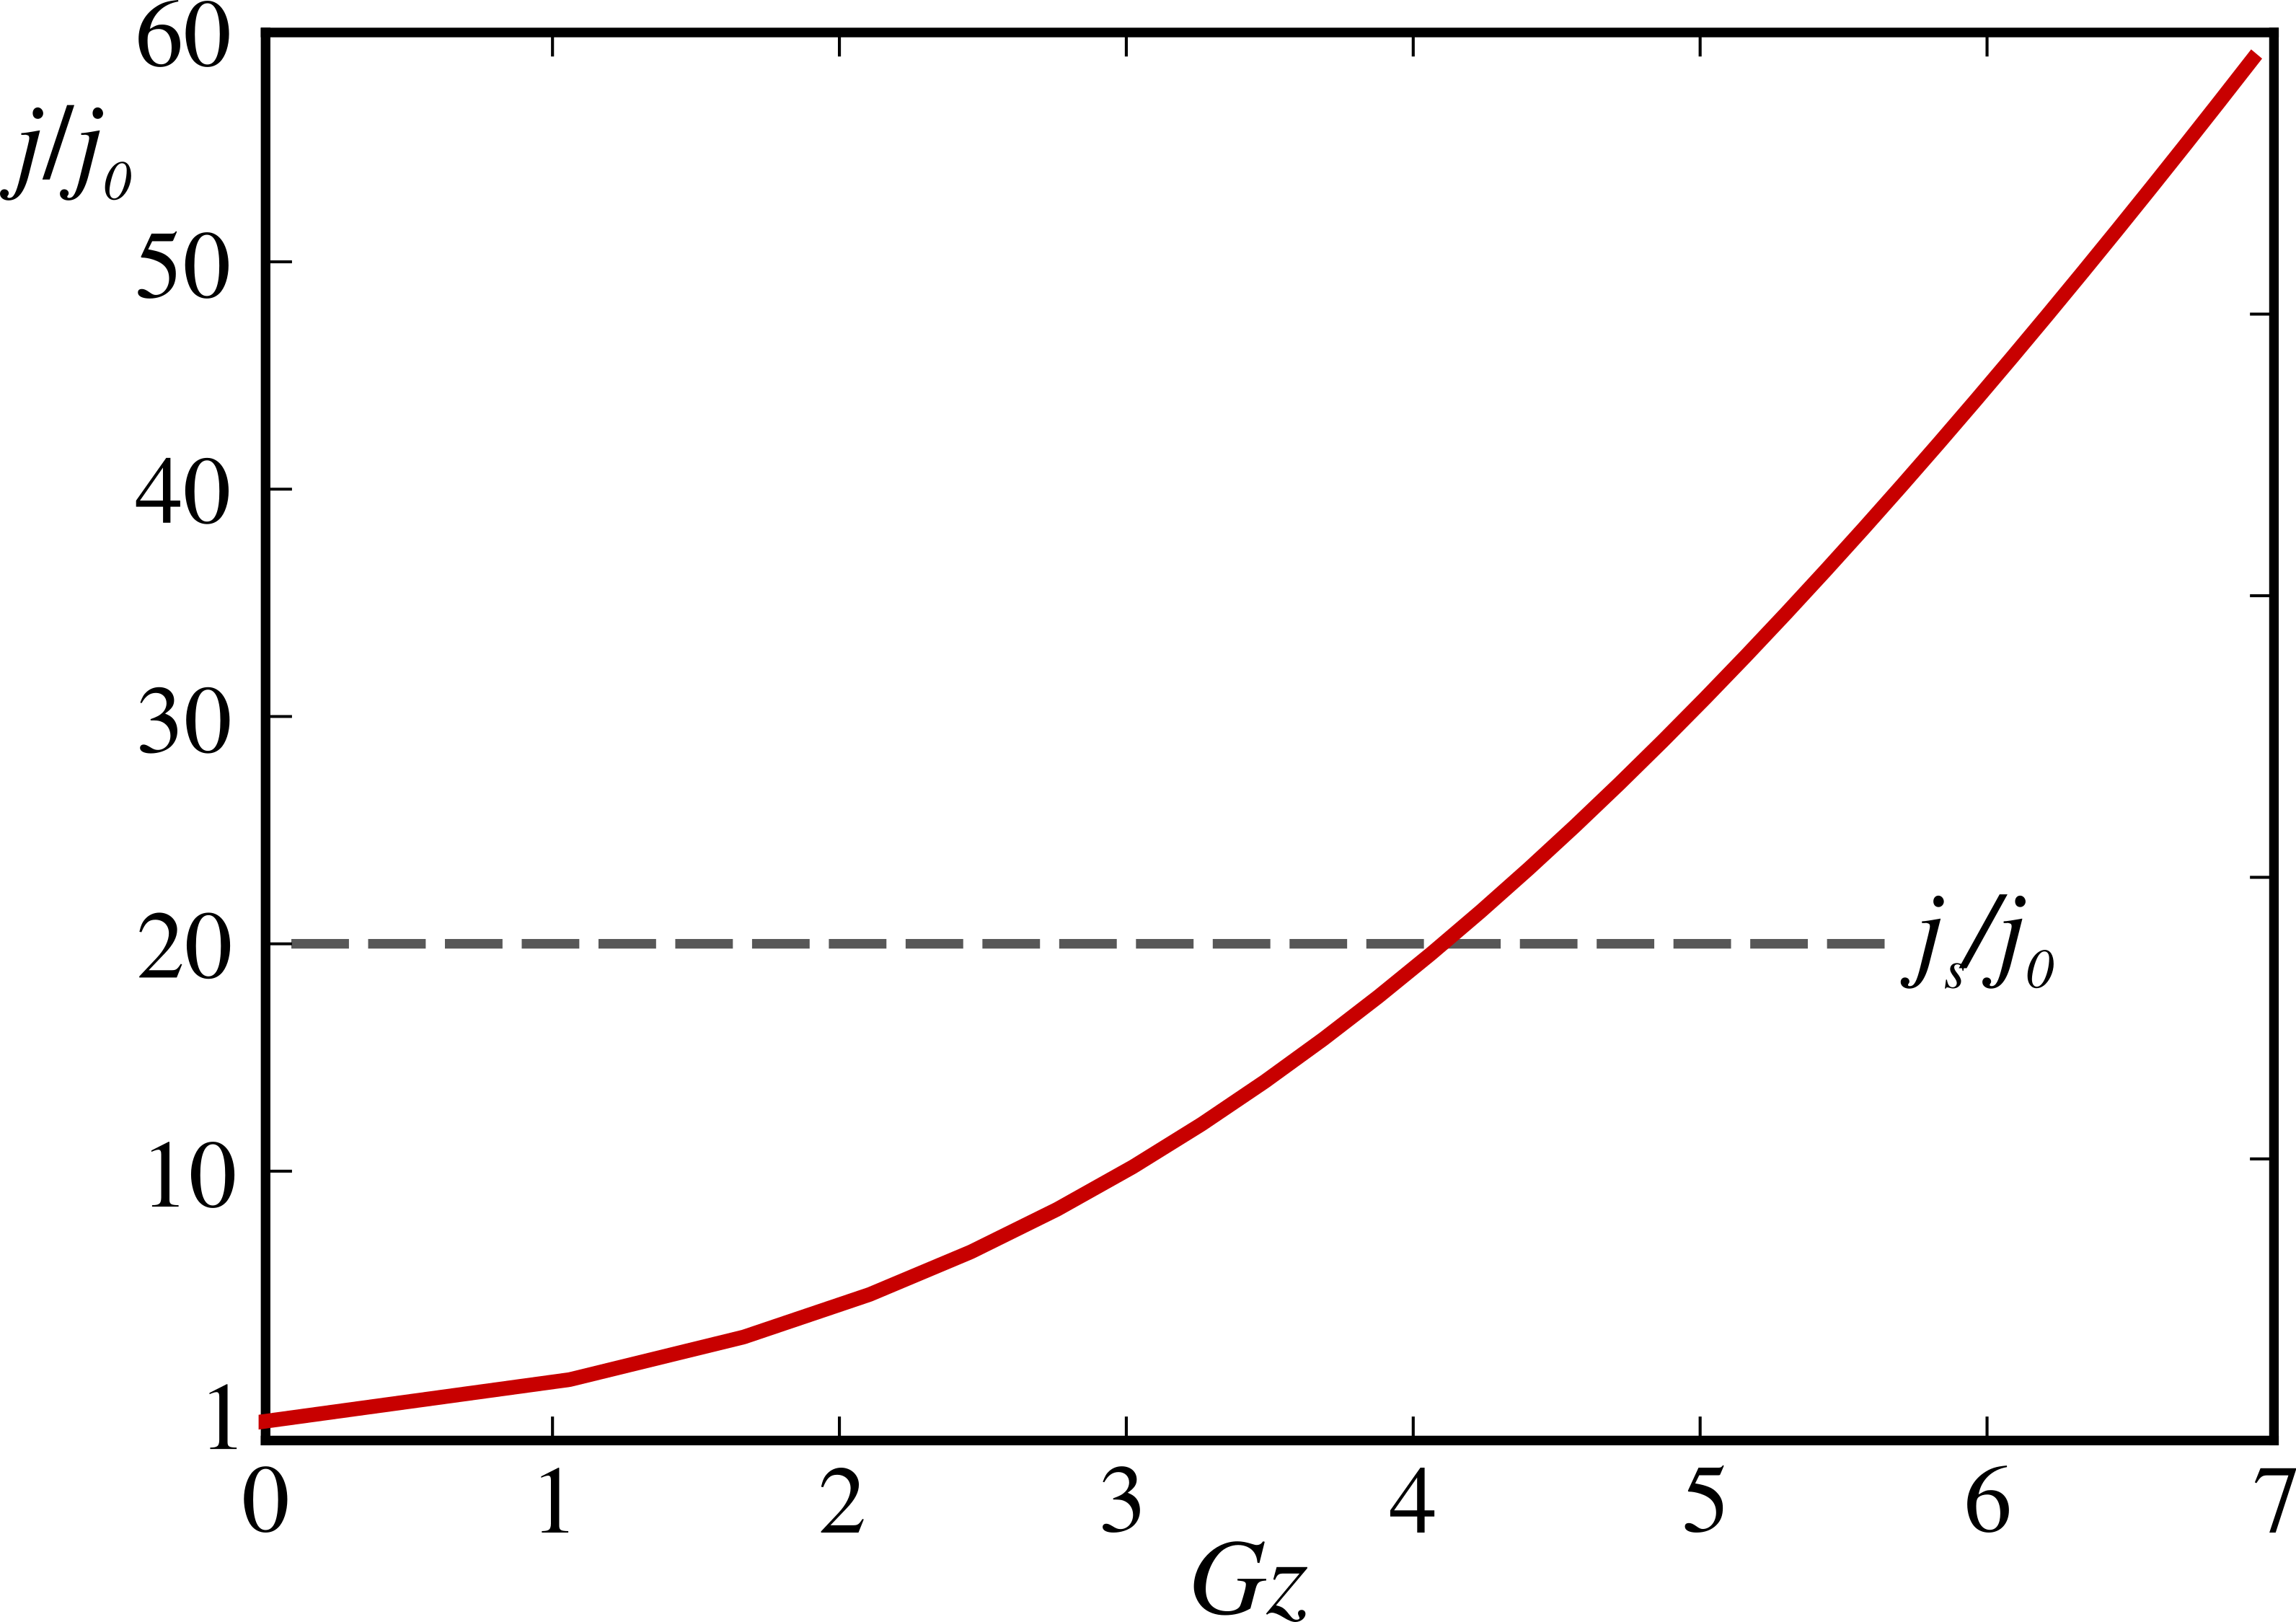
\includegraphics[width=8truecm]{slike/05_joja.png}
\caption{Naraščanje gostote svetlobnega toka pri optičnem ojačanju}
\label{fig:ojacanje}
\end{figure}


Obnašanje gostote svetlobnega toka ima, tako kot pri absorpciji, dva režima. 
Pri majhnih gostotah toka $j\ll j_{s}$ je naraščanje eksponentno 
\begin{equation}
j(z)=j_{0}e^{Gz}.
\label{4.45}
\end{equation}
Pri velikih gostotah toka pride do nasičenja in gostota svetlobnega
toka se ojačuje linearno z razdaljo
\begin{equation}
j(z)=\tilde{j_{0}}+j_{s}Gz=\tilde{j_{0}}+\frac{rN}{V}\hbar \omega z.
\label{4.46}
\end{equation}
 V tem primeru je gostota toka dovolj velika, da vsi atomi, ki jih
s črpanjem spravimo v najvišje stanje, preidejo v stanje $|1\rangle$
s stimuliranim sevanjem. Pri konstantnem črpanju je tedaj 
linearno naraščanje gostote toka razumljivo. 

\section{Homogena in nehomogena razširitev spektralne črte}
\label{Razsiritev}
Doslej smo predpostavili, da svetijo vsi atomi obravnavane snovi
pri isti frekvenci $\omega_{0}$ in z isto spektralno širino, ki smo
jo popisali s funkcijo $g(\omega)$, z vrhom pri $\omega_0$. Če to drži, 
pravimo, da je razširitev spektralne črte homogena\index{Spektralna črta!homogena razširitev}. 
Primera homogene razširitve sta naravna širina in razširitev zaradi trkov med atomi. 
Funkcija $g(\omega)$ je v tem primeru Lorentzove oblike
\beq
g(\omega)=\frac{1}{\pi}\frac{\gamma}{(\omega-\omega_{0})^{2}+\gamma^{2}}
\eeq
s širino črte $\gamma$. 

% %izračunaj širino zaradi trkov v HeNE laserju. Tlak p, molska masa M, 
% collision time tc sqrt(2/3 MkT)/8 pi pa^2.
% pri 0.5 atm, tc 0.5 mus, delta ni 0.64 MHz << 5 10^14 hz. 
% Primerjaj z naravno širino, = kako sešteješ.
% 
% Nehomogena razširitev - Gauss, impurities v steklu, local elektctic field, 
% Stark shift, NdGlass, 5.4 THz, 
% 
% Doppler / Gauss.HenE 1.7 GHz
% 
% Seštevanje razširitev s konvolucijo int g*(x) g(omega - omega 0-x) dx
% voigt funkcija
% če dva homogena, delta je vsota delta.
% če dva nehomogena delata je sqrt delta^2


Spektralna črta je lahko razširjena tudi zato, ker vsi atomi ne svetijo
pri povsem enaki frekvenci. Tedaj govorimo o nehomogeni 
razširitvi\index{Spektralna črta!nehomogena razširitev}.
Najpomembnejši primer nehomogene razširitve je Dopplerjeva 
\index{Dopplerjeva razširitev} razširitev v plinu. 
Atomi plina vedno sevajo pri praktično isti frekvenci, vendar jih zaradi gibanja
opazovalec v mirujočem (laboratorijskem) sistemu v skladu z Dopplerjevim pojavom 
zazna pri različnih frekvencah. Tako so frekvence $\omega$ posameznih atomov 
odvisne od hitrosti $v$ atoma glede na smer opazovanja. Zapišemo jih kot  
\begin{equation}
\omega=\omega_{0}-\frac{v}{c}\omega_{0}=\omega_{0}-k_{0}v.
\label{4.81}
\end{equation}
Označimo z ${\cal N}(v)$ porazdelitev gostote atomov po hitrostih
v smeri opazovanja. V termičnem ravnovesju je ${\cal N}(v)$ Maxwellova
porazdelitev
\begin{equation}
{\cal N}(v)=\frac{N}{V}\left(\frac{m}{2\pi k_{B}T}\right)^{1/2}e^{-\frac{mv^{2}}{2k_{B}T}}.
\label{4.82}
\end{equation}
 Porazdelitev atomov po frekvencah dobimo tako, da hitrost izrazimo
iz enačbe~(\ref{4.81}), pri čemer dobljeno funkcijo $g_{D}(\omega)$
normiramo tako. Dobimo
\begin{equation}
g_{D}(\omega)=\frac{c}{\omega_{0}}\left(\frac{m}{2\pi 
k_{B}T}\right)^{1/2}e^{-\frac{mc^{2}}{2k_{B}T}\frac{(\omega-\omega_{0})^{2}}{\omega_{0}}}.
\label{4.821}
\end{equation}
Dopplerjeva razširitev v plinu je torej Gaussove oblike. Njena širina pri polovični 
višini\footnote{To širino imenujemo FWHM -- \it{Full width at half maximum}.} je
\begin{equation}
\Delta\omega_{D}=2 \sqrt{\frac{2k_{B}T \ln 2}{mc^{2}}}\omega_{0}.
\label{4.83}
\end{equation}
\begin{definition}
Izpelji obliko nehomogeno razširjene črte za Dopplerjevo razširitev (enačba~\ref{4.821})
in pokaži, da je njena širina podana z enačbo~(\ref{4.83}).
\end{definition}


Izračunajmo Dopplerjevo razširitev na primeru He-Ne laserja. Za prehod
atoma neona pri 632,8~nm in temperaturi 300~K dobimo 
$\Delta\omega_{D}=8\times10^{9}~\hertz$. Nehomogena Dopplerjeva razširitev v 
redkem plinu je navadno nekaj redov velikosti večja od homogene naravne širine in 
razširitve zaradi trkov.

% \section{*Nasičenje nehomogeno razširjene absorpcijske črte}
% 
% V razdelku~(\ref{chap:NasAbs}) smo obravnavali nasičenje absorpcije pri homogeno 
% razširjenem prehodu. Pri nasičenju absorpcije, kadar prevladuje nehomogena razširitev,
% nastopijo pomembni novi pojavi, zato si to podrobneje oglejmo.
% 
% 
% Naj na plin vpada močan snop monokromatske svetlobe s frekvenco $\omega$,
% ki je blizu osrednje frekvence $\omega_{0}$ Dopplerjevo razširjene črte. S svetlobo
% lahko sodeluje le skupina atomov, pri kateri se Dopplerjevo premaknjena
% frekvenca od $\omega$ ne razlikuje več kot za homogeno širino, ki
% jo opisuje funkcija $g(\omega)$. Zato ne moremo zapisati zasedbenih
% enačb za vse atome hkrati, ampak le za tiste, ki imajo hitrost med
% $v$ in $v+dv$ in ki absorbirajo pri frekvenci $\omega_{0}-kv$.
% 
% 
% Naj sta ${\cal N}_{1}(v)$ in ${\cal N}_{2}(v)$ hitrostni porazdelitvi
% atomov v spodnjem in v zgornjem stanju. Enačba za spreminjanje gostote
% ${\cal N}_{2}(v)$ je analogna enačbi~(\ref{4.22}) za celotno
% zasedenost v homogenem primeru
% \begin{equation}
% \frac{d{\cal N}_{2}(v)}{dt}=-A{\cal N}_{2}(v) -B\, g(\omega-\omega_{0}+kv)
% \frac{j_{\omega}}{c}\,
% [{\cal N}_{2}(v)-{\cal N}_{1}(v)],
% \label{4.85}
% \end{equation}
%  kjer je $j_{\omega}$ gostota vpadnega svetlobnega toka. Upoštevali
% smo, da je zaradi Dopplerjevega pojava prehod premaknjen k frekvenci
% $\omega_{0}-kv$. Velja tudi
% \begin{equation}
% {\cal N}_{1}(v)+{\cal N}_{2}(v)={\cal N}(v)\mbox{\hskip1cm in \hskip1cm}\frac{d{\cal N}_{2}(v)}{dt}=-\frac{d{\cal N}_{1}(v)}{dt}.
% \label{4.86}
% \end{equation}
% Vpeljimo ${\cal Z}(v)={\cal N}_{2}(v)-{\cal N}_{1}(v)$. Podobno kot 
% v enačbi~(\ref{4.321}) zapišemo
% \beq
% {\cal N}_{2}(v)=1/2{\cal N}(v)+1/2{\cal Z}(v)
% \eeq
% in dobimo 
% \begin{equation}
% \dot{{\cal Z}}(v)=-A{\cal Z}(v)-A{\cal N}(v)
% -2B\,g(\omega-\omega_{0}+kv)\frac{j_{\omega}}{c}
% {\cal Z}(v).
% \label{4.87}
% \end{equation}
% V stacionarnem stanju je 
% \begin{equation}
% {\cal Z}(v)=\frac{{\cal N}(v)}{1+\frac{2B}{Ac}g(\omega-\omega_{0}+kv)j_{\omega}}.\label{4.88}
% \end{equation}
%  Če je nasičenje majhno, lahko imenovalec v gornji enačbi razvijemo
% \begin{equation}
% {\cal Z}(v)\simeq{\cal N}(v)[1-\frac{2B}{Ac}g(\omega-\omega_{0}+kv)j_{\omega}].\label{4.89}
% \end{equation}
%  Porazdelitev ${\cal Z}(v)$je podobna nemoteni porazdelitvi atomov
% po hitrosti ${\cal N}(v)$, le da je pri hitrosti $v=(\omega_{0}-\omega)/k$
% zmanjšana zaradi vpliva vpadne svetlobe, ki jo atomi s to hitrostjo
% lahko absorbirajo in s tem prehajajo v gornje stanje. V porazdelitvi
% atomov v spodnjem stanju tako nastane vdolbina, pravijo ji tudi Bennetova
% vdolbina, v gornjem stanju, ki je bilo na začetku prazno, pa dobimo
% ustrezen ozek vrh (Slika \ref{***}). Širina vdolbine je določena
% s homogeno širino prehoda, to je s funkcijo $g(\omega-\omega_{0}+kv)$,
% globina pa z gostoto vpadnega toka.
% 
% Zapišimo sedaj absorpcijski koeficient pri neki frekvenci $\omega^{\prime}$,
% ki ga izmerimo tako, da na plin posvetimo z dodatnim, šibkim testnim
% snopom. Upoštevati moramo, da k absorpciji prispevajo vsi atomi, katerih
% hitrost je taka, da je prehod dovolj blizu $\omega^{\prime}$. Zato
% dobimo absorpcijski koeficient s seštevanjem po porazdelitvi ${\cal Z}(v)$
% \begin{equation}
% \mu(\omega^{\prime})=\frac{\hbar\omega^{\prime}}{c}\int{\cal Z}(v)Bg(\omega^{\prime}-\omega_{0}+k^{\prime}v)\, dv\label{4.90}
% \end{equation}
%  Homogena razširitev je navadno dosti manjša od Dopplerjeve širine.
% V prvem približku vzemimo, da lahko $g(\omega)$ nadomestimo kar z
% $\delta(\omega)$, pri čemer to ne smemo narediti tudi v imenovalcu
% izraza za ${\cal Z}(v)$. Tako dobimo 
% \begin{eqnarray}
% \mu(\omega^{\prime}) & = & \frac{\hbar\omega^{\prime}}{k^{\prime}c}B\frac{{\cal N}(\frac{\omega^{\prime}-\omega0}{k})}{1+\frac{2B}{Ac}g(\omega-\omega^{\prime})j_{\omega}}\nonumber 
%  & \simeq & \hbar B{\cal N}(\frac{\omega^{\prime}-\omega0}{k})[1-\frac{2B}{Ac}g(\omega-\omega^{\prime})j_{\omega}].
% \end{eqnarray}
%  V drugi vrstici smo uporabili približek \ref{4.89}. Odvisnost $\mu(\omega^{\prime})$,
% ki jo izmerimo tako, da spreminjamo frekvenco testnega snopa $\omega^{\prime}$,
% je Gaussove oblike z vdolbino pri $\omega$ in je podobna porazdelitvi
% ${\cal Z}(v)$, kot jo kaže slika \ref{***}. Vdolbina ima obliko
% homogeno razširjene črte. Merjenje nasičenja absorpcije s testnim
% žarkom torej omogoča dobiti obliko homogene črte kljub mnogo večji
% nehomogeni Dopplerjevi razširitvi in je zato v moderni spektroskopiji
% velikega pomena.
% 
% Absorpcijski koeficient za prvi, močan vpadni snop dobimo s tem, da
% v gornjem izrazu postavimo $\omega^{\prime}=\omega$. ${\cal N}((\omega-\omega^{\prime})/k)$
% opisuje običajno Gaussovo obliko Dopplerjevo razširjene črte, izraz
% v oglatem oklepaju pa da zmanjšanje absorpcije zaradi nasičenja, ki
% je odvisno le od vrednosti $g(0)$ in zato enako pri vseh $\omega$.
% Z enim samim snopom izmerjena črta je kljub nasičenju še vedno Gaussove
% oblike. Vdolbina, ki jo izžge svetloba v hitrostni porazdelitvi atomov,
% s takim preprostim opazovanjem ne moremo zaznati.
% 
% Namesto z dvema različnima snopoma, od katerih lahko enemu spreminjamo
% frekvenco, lahko vdolbino v porazdelitvi zaznamo tudi z enim snopom
% spremenljive frekvence, ki se po prvem prehodu skozi plin odbije od
% ogledala in vrne v nasprotni smeri. S tem se v porazdelitvi atomov
% v spodnjem stanju simetrično pri hitrostih $\pm(\omega_{0}-\omega)/k$
% pojavita dve vdolbini. Kadar je $\omega$ blizu $\omega_{0}$, se
% začneta obe vdolbini prekrivati, stopnja nasičenja se poveča in s
% tem se celotna absorpcija po dveh prehodih zmanjša (Slika \ref{***}).
% 
% Zapišimo še enačbe za ta primer. Snop povzroči spremembo zasedenosti
% pri prehodu skozi plin v obeh smereh, zato je sedaj 
% \begin{equation}
% {\cal Z}(v)\simeq{\cal N}(v)\{1-\frac{2B}{Ac}j_{\omega}[g(\omega-\omega_{0}+kv)+g(\omega-\omega_{0}-kv)]\}.\label{4.92}
% \end{equation}
%  Enako kot prej je absorpcijski koeficient za širjenje svetlobe v
% pozitivni smeri 
% \begin{eqnarray}
% \mu_{+}(\omega) & = & \frac{\hbar\omega}{c}B\int{\cal Z}(v)g(\omega-\omega_{0}+kv)\, dv\nonumber \\
%  & \simeq & \hbar B{\cal N}(\frac{\omega-\omega0}{k})\{1-\frac{2B}{Ac}[g(0)+g(2(\omega-\omega_{0}))]j_{\omega}\}\;.
% \end{eqnarray}
%  Ker je ${\cal Z}(v)={\cal Z}(-v)$, je izraz za absorpcijo v negativni
% smeri enak. Pri $\omega=\omega_{0}$ je nasičenje večje in absorpcija
% se zato zmanjša. Izmerjeni absorpcijski profil ima na sredini vdolbino,
% ki je zopet podobna homogeno razširjeni črti. Faktor 2 v argumentu
% funkcije $g(2(\omega-\omega_{0}))$ je posledica našega grobega približka,
% ko smo v integraciji $g(\omega-\omega_{0}+kv)$ nadomestili kar z
% $\delta$ funkcijo. Natančnejši račun pokaže, da je vrh pri $\omega_{0}$
% kar oblike $g(\omega-\omega_{0})$ (Naloga).


\section{Izpeljava verjetnosti za prehod}
\label{chap:verjetnost}
Verjetnosti za prehod atoma iz enega stanja v drugo s sevanjem, ki
smo jih opisali s fenomenološkimi Einsteinovimi koeficienti $A_{21}$
in $B_{21}$ (razdelek~\ref{AB}), je mogoče izpeljati tudi drugače.
Pri tem se poslužimo kvantne elektrodinamike, kar pomeni kvantno obravnavo 
tako atoma kot elektromagnetnega polja. Povsem strog račun je zahteven in presega
okvir te knjige, zato si na kratko oglejmo le, kako pridemo do rezultata s
perturbacijsko metodo.


Postavimo dvonivojski atom v votlino z elektromagnetnim poljem.
Izračunajmo verjetnost, da zaradi interakcije s poljem atom
preide iz stanja $|2\rangle$ v stanje $|1\rangle$, pri čemer se
število fotonov v izbranem stanju elektromagnetnega polja $\alpha$
poveča z $n_{\alpha}$ na $n_{\alpha}+1$. V vseh ostalih stanjih
polja naj bo število fotonov enako nič.


Med atomom in poljem privzemimo električno dipolno interakcijo 
\begin{equation}
\hat{H}_{i}=-e\hat{E}(\mathbf{r},t)\hat{x},
\label{4.47}
\end{equation}
kjer je $\hat{x}$ operator koordinate elektrona v atomu. Privzeli
smo, da je nihajoče polje polarizirano v smeri osi $x$. Stanja celotnega sistema, 
to je atoma in polja, zapišimo v obliki produkta atomskih stanj in
stanja elektromagnetnega polja, pri čemeer moramo navesti število fotonov
v vsakem nihanju votline $\alpha$
\begin{equation}
|i,\{n_{\alpha}\}\rangle\equiv|i\rangle|\{n_{\alpha}\}\rangle.
\label{4.48}
\end{equation}
Začetno stanje celotnega sistem naj bo tako $|2,n_{\alpha}\rangle$, kar pomeni, da je
atom v gornjem stanju, polje pa ima $n_{\alpha}$ fotonov v enem samem stanju $\alpha$.
Ustrezno končno stanje je $|1,n_{\alpha}+1\rangle$.


V prvem redu teorije motenj je verjetnost za prehod iz začetnega v končno stanje
na časovno enoto enaka
\begin{equation}
w_{21}=\frac{2\pi}{\hbar}|\langle1,n_{\alpha}+
1|\,\hat{H}_{i}\,|2,n_{\alpha}\rangle|^{2}\,
\delta(E_{2}-E_{1}-\hbar\omega_{\alpha}).
\label{4.49}
\end{equation}
Z delta funkcijo izberemo le prehoda, pri katerih se ohranja
energija.


Operator elektromagnetnega polja lahko po enačbi~(\ref{eq:pqrazvoj}) 
razvijemo po lastnih nihanjih votline 
\begin{equation}
\hat{E}(\mathbf{r},t)=-\frac{1}{\sqrt{V\epsilon_{0}}}\sum_{\alpha}
\hat{p}_{\alpha}(t)E_{\alpha}(\mathbf{r}),
\label{4.50}
\end{equation}
kjer je $\hat{p}_{\alpha}$ operator impulza nihanja $\alpha$, $E_{\alpha}$
pa funkcija, ki popisuje krajevno odvisnost polja. Vemo, da se vsako 
elektromagnetno nihanje votline obnaša kot harmonski oscilator.
Zato lahko vpeljemo kreacijske in anihilacijske operatorje
\begin{eqnarray}
\hat{a}_{\alpha}^{\dagger} & = & \frac{1}{\sqrt{2\hbar\omega_{\alpha}}}\,
(\omega_{\alpha}\hat{q}_{\alpha}-i\hat{p}_{\alpha}) \\
\hat{a}_{\alpha} & = & \frac{1}{\sqrt{2\hbar\omega_{\alpha}}}\,(\omega_{\alpha}\hat{q}_{\alpha}+i\hat{p}_{\alpha}).
\end{eqnarray}
 Kreacijski operatorji povečujejo, anihilacijski pa znižujejo število
fotonov v danem stanju
\begin{eqnarray}
\hat{a}_{\alpha}^{\dagger}|n_{\alpha}\rangle & = & \sqrt{n_{\alpha}+1}
|n_{\alpha}+1\rangle\qquad \mathrm{in} \\
\hat{a}_{\alpha}|n_{\alpha}\rangle & = & \sqrt{n_{\alpha}}|n_{\alpha}-1\rangle.
\end{eqnarray}
Edini od nič različni matrični elementi so tako oblike
\begin{eqnarray}
\langle n_\alpha +1|\, \hat{a}_{\alpha}^{\dagger}\,|n_{\alpha}\rangle & = 
& \sqrt{n_{\alpha}+1} \qquad \mathrm{in} \nonumber\\
\langle n_\alpha-1|\,\hat{a}_{\alpha}\,|n_{\alpha}\rangle & = & \sqrt{n_{\alpha}}.
\label{eq:ankr}
\end{eqnarray}
Operatorje $\hat{p}_{\alpha}$ zdaj lahko izrazimo s kreacijskimi in anihilacijskimi
operatorji in jih vstavimo v razvoj električnega polja (enačba~\ref{4.50}). Dobimo
\begin{equation}
\hat{E}(\mathbf{r},t)=-i\sum_{\alpha}\sqrt{\frac{\hbar\omega_{\alpha}}{2V\epsilon_{0}}}\,
\left(\hat{a}_{\alpha}^{\dagger}-\hat{a}_{\alpha}\right)E_{\alpha}(\mathbf{r}).
\label{4.53}
\end{equation}
Nadaljujemo z izračunom potrebnega matričnega elementa. Operator koordinate
$\hat{x}$ deluje le na atomski del stanja, $\hat{E}$ pa le na elektromagnetno
polje, zato velja 
\begin{eqnarray}
\langle1,n_{\alpha}+1|\,\hat{H}_{i}\,|2,n_{\alpha}\rangle & = & -e\,
\langle1,n_{\alpha}+1|\,\hat{E}\,\hat{x}\,|2,n_{\alpha}\rangle \\
 & = & -e\,\langle1|\,\hat{x}\,|2\rangle\langle n_{\alpha}+1|\,\hat{E}\,|n_{\alpha}\rangle.
\end{eqnarray}
Vstavimo polje, ki smo ga izrazili s kreacijskimi in anihilacijskimi operatorji (enačba~\ref{4.53}),
upoštevamo zvezi~(\ref{eq:ankr}) in dobimo
\begin{eqnarray}
\langle n_{\alpha}+1|\, \hat{E}\,|n_{\alpha}\rangle & = 
& -i\sum_{\beta}\sqrt{\frac{\hbar\omega_{\beta}}{2V\epsilon_{0}}}
\langle n_{\alpha}+1|\,\hat{a}_{\beta}^{\dagger}-\hat{a}_{\beta}\,|n_{\alpha}\rangle\, 
E_{\beta}(\mathbf{r})\nonumber \\
 & = & -i\sqrt{\frac{\hbar\omega_{\alpha}}{2V\epsilon_{0}}}
 \sqrt{n_{\alpha}+1}\, E_{\alpha}(\mathbf{r}).
\end{eqnarray}
Od vseh operatorjev v razvoju polja dobimo namreč od nič različen matrični
element le za kreacijski operator za stanje $\alpha$.


Vpeljimo še simbol za matrični element koordinate med 
atomskimi stanji $\langle1|\hat{x}|2\rangle=x_{12}$. Iskana verjetnost za prehod iz 
začetnega stanja, v katerem smo imeli vzbujen atom in $n_{\alpha}$ fotonov, v končno
stanje z atomom v osnovnem stanju in $n_{\alpha}+1$ fotonov v stanju $\alpha$ je tako
\begin{equation}
w_{21}=\frac{\pi e^{2}\omega_{\alpha}x_{12}^{2}}{V\epsilon_{0}}
(n_{\alpha}+1)\,E_{\alpha}^{2}(\mathbf{r})\,\delta(E_{2}-E_{1}-\hbar\omega_{\alpha}).
\label{4.56}
\end{equation}
Verjetnost za prehod je sorazmerna z $n_{\alpha}+1$ in je od nič
različna, tudi če je število kvantov polja enako nič. Tedaj imamo seveda
spontano sevanje\index{Spontano sevanje}. Prispevek, ki je 
sorazmeren s številom že prisotnih fotonov, pa predstavlja stimulirano 
sevanje\index{Stimulirano sevanje}. Prehodna verjetnost vsebuje
še kvadrat prostorske odvisnosti polja $E_{\alpha}^{2}(\mathbf{r})$.
Če ne poznamo natančnega položaja atoma ali če imamo plin atomov, ki je enakomerno
porazdeljen po votlini, lahko ta člen nadomestimo kar s povprečno vrednostjo.
Kadar imamo stoječe valovanje, je to 1/2.


Spontana emisija je možna v vsa elektromagnetna nihanja votline s
pravo frekvenco. Celotno verjetnost za prehod atoma iz vzbujenega
v osnovno stanje dobimo, če seštejemo verjetnosti za prehod z izsevanim fotonom 
v določenem stanju. Spomnimo se, da je ta verjetnost ravno enaka 
Einsteinovem koeficientu $A_{21}$\index{Einsteinovi koeficienti} (enačba~\ref{4.27})
\begin{equation}
A_{21}=\sum_{\alpha}w_{21}=\sum_{\alpha}\frac{\pi 
e^{2}\omega_{\alpha}x_{12}^{2}}{2V\epsilon_{0}}\,\delta(E_{2}-E_{1}-\hbar\omega_{\alpha}).
\label{4.57}
\end{equation}
Za prostorsko odvisnost polja $E^{2}(\mathbf{r})$ smo vzeli povprečje
1/2. Vsoto po nihanjih lahko z uporabo enačbe~(\ref{4.5}) spremenimo v integral
in upoštevamo enačbo~(\ref{4.4}). Dobimo
\begin{equation}
A_{21}=\frac{\pi e^{2}x_{12}^{2}}{2\hbar\epsilon_{0}}\int\rho(\omega_{\alpha})\omega_\alpha\, 
\delta(\omega_{0}-\omega_{\alpha})\, d\omega_{\alpha}=\frac{e^{2}\omega_{0}^{3}x_{12}^{2}}{2\pi\epsilon_{0}\hbar c^{3}}.
\label{4.58}
\end{equation}
 Z $\omega_{0}=(E_{2}-E_{1})/\hbar$ smo označili frekvenco prehoda. S tem smo 
 izpeljali vrednost Einsteinovega koeficienta $A_{21}$. 
 

Zaradi spontanega sevanja vzbujeno atomsko stanje ne more biti popolnoma
stacionarno. Poleg tega energija stanja s končnim razpadnim časom ni natančno
določeno. Zato moramo verjetnost za stimulirano sevanje (enačba~\ref{4.56}) malo 
popraviti. Delta funkcijo energije nadomestimo s končno široko funkcijo $g(\omega)$, 
ki ima vrh pri $\omega_{0}$ in je njen integral enak 1. Pri tem dobimo zaradi 
spremembe integracijske spremenljivke še en dodaten faktor $1/\hbar$. Tako imamo 
\begin{equation}
w_{21}=\frac{\pi e^{2}\omega_{\alpha}x_{12}^{2}}{2V\epsilon_{0}\hbar}
(n_{\alpha}+1)g(\omega_{\alpha}).
\label{4.59}
\end{equation}
Einsteinov koeficient za stimulirano sevanje lahko izrazimo iz enačbe~(\ref{4.18}), 
če upoštevamo, da je gostota energije polja $n_{\alpha}\hbar\omega_{\alpha}/V$
\begin{equation}
B_{21}g(\omega_{\alpha})=\frac{Vw_{21}}{n_{\alpha}\hbar\omega_{\alpha} g(\omega_{\alpha})}
=\frac{\pi e^{2}x_{12}^{2}}{2\epsilon_{0}\hbar^{2}}.
\label{4.60}
\end{equation}
Poglejmo  še razmerje izračunanih Einsteinovih koeficientov iz enačb~(\ref{4.58}) in 
(\ref{4.60}). Vidimo, da se ujema z razmerjem, ki smo ga izpeljali z uporabo
Planckove formule (enačba~\ref{4.27}). Prehojena pot jasno kaže zvezo med spontanim in
stimuliranim sevanjem ter gostoto stanj elektromagnetnega polja. 

%Še branje

%-------------------------------------------------------------------------------
%	CHAPTER 6
%-------------------------------------------------------------------------------

\chapterimage{slike/Navy.jpg} 
\chapter{Laser}

V prejšnjih poglavjih smo spoznali resonatorje, pojasnili proces ojačevanja svetlobe in 
opisali črpanje, ki je potrebno za vzdrževanje obrnjene zasedenosti v ojačevalnem sredstvu. 
V tem poglavju bomo vsa ta
spoznanja združili in komponente sestavili v eno samo napravo -- laser. Zapisali
bomo zasedbene enačbe, pojasnili delovanje laserjev in spoznali prednosti 
laserske svetlobe pred svetlobo iz navadnih svetil. Opisali bomo način delovanja 
sunkovnih laserjev in na koncu predstavili semiklasični model laserja. 

\section{Laser}
\index{Laser}\index{Spontano sevanje}
\index{Optično ojačevanje}
V sredstvu, v katerem med dvema nivojema dosežemo obrnjeno 
zasedenost, se svetloba z ustrezno valovno dolžino ojačuje. 
Postavimo tako sredstvo v optični resonator. \index{Resonator} 
Na začetku nastaja predvsem spontano izsevana svetloba in 
v resonatorju se vzbujajo tista lastna nihanja, katerih frekvenca je blizu frekvence
atomskega prehoda. Resonator poskrbi, da se svetloba odbija nazaj v ojačevalno 
sredstvo. Če v njem vzdržujemo obrnjeno zasedenost, se svetloba ob prehodu skozi 
sredstvo ojačuje.
V začetku je ojačenje za
izbrana nihanja veliko, z naraščajočo intenziteto pa se ojačenje zmanjšuje.
\index{Izgube v resonatorju} 
Ko se ojačenje na prelet izenači z izgubami, sistem preide v stacionarno stanje in 
seva močno koherentno svetlobo. Tak
izvor svetlobe imenujemo laser. Beseda laser je nastala iz kratice za {\it Light
Amplification by Stimulated Emission of Radiation} --  ojačenje svetlobe s
stimuliranim sevanjem.

\begin{figure}[h]
\centering
\def\svgwidth{100truemm} 
\input{slike/06_shema.pdf_tex}
\caption{Shema laserja s ključnimi deli: ojačevalno sredstvo, črpalni mehanizem in resonator}
\label{fig:shemalaserja}
\end{figure}
\begin{remark}
Kot klasično analogijo za laser vzamemo klarinet, ki je sestavljen iz 
cevi in ustnika. Cev deluje kot resonator, v katerem nastane 
stoječi zvočni val, pri čemer je frekvenca stoječega vala določena z 
dolžino cevi in s številom vozlov. Naloga ustnika je dovajanje energije 
in s tem vzdrževanje konstantne amplitude nihanja. To glasbenik doseže s 
pihanjem v ustnik in tresenjem prožnega jezička, ki s tresljaji proizvaja 
zvok. Tresenje jezička je približno periodično in vsebuje mnogo različnih 
frekvenc, tudi take, ki ustrezajo frekvenci stoječih valov v cevi. 
Ko amplituda tlaka v cevi naraste nad neko mejo, nastopi zanimiv
pojav. Nihanje tlaka v gornjem koncu cevi povratno deluje na ustnik
in ga sili, da niha s frekvenco najmočneje vzbujenega stoječega vala v cevi,
druge frekvence pa zamrejo. Moč pihanja gre le še v
nihanje jezička s pravo frekvenco in ojačuje nihanje zračnega stolpca. 
Tako se s povratno zvezo med nihanjem jezička in stoječim valovanjem v cevi
vzdržuje stoječe valovanje s konstantno amplitudo. 
\end{remark}

V grobem ima laser tri ključne sestavne dele: ojačevalno sredstvo, 
črpalni mehanizem in resonator, ki je v najpreprostejšem primeru sestavljen iz dveh 
ukrivljenih zrcal (slika~\ref{fig:shemalaserja}). Črpalni \index{Črpanje}
mehanizem vzdržuje obrnjeno zasedenost v ojačevalnem sredstvu, medtem ko resonator 
omogoča, da se svetloba med številnimi prehodi skozi ojačevalno sredstvo dovolj ojači.
Odbojnost vsaj enega od zrcal 
mora biti manjša od 1, da skozenj lahko izhaja svetloba.

Zaenkrat se omejimo na najpreprostejši model laserja in 
privzamemo, da frekvenca le enega resonatorskega lastnega nihanja sovpada s 
frekvenco prehoda aktivne snovi. Ta predpostavka v večini laserjev ni
avtomatično izpolnjena, vendar jo je pogosto mogoče doseči z dodatnimi elementi 
v resonatorju. Aktivno snov oziroma ojačevalno sredstvo v laserju stalno 
črpamo in s tem vzdržujemo obrnjeno zasedenost. 

Naj bo $W$ energija svetlobnega valovanja v resonatorju. Zaradi izgub skozi
zrcali in zaradi absorpcije ter sipanja v resonatorju se energija na en obhod 
resonatorja zmanjša za (enačba~\ref{eq:Lambda})
\begin{equation}
\Delta W_{\rm izgube}=-\Lambda W=-\left(1-{\cal {R}}_{1}+1-{\cal {R}}_{2}
+2\alpha L\right)W,
\label{5.1}
\end{equation}
kjer so $\Lambda $ celotne izgube, $\alpha$ izgube na enoto poti zaradi
absorpcije in sipanja, $L$ je dolžina resonatorja ter \index{Izgube v resonatorju}
${\cal {R}}_{1}$ in ${\cal {R}}_{2}$ odbojnosti
zrcal. V ojačevalnem sredstvu, v katerem vzdržujemo obrnjeno zasedenost,
pride do ojačevanja s stimuliranim sevanjem. Energija nihanja resonatorja 
se tako na en obhod po enačbi (\ref{eq:djG}) poveča za 
\index{Ojačevanje s stimuliranim sevanjem|see{Stimulirano sevanje}}
\begin{equation}  
\Delta W_{\rm oja\check{c}enje}=\frac{G}{1+W/W_s}\,W\, 2L'.
\label{5.2}
\end{equation}
Vpeljali smo saturacijsko energijo $W_s=Vj_s/c$, $G$ pa je koeficient ojačenja.
Dolžino ojačevalnega sredstva,
ki se v splošnem razlikuje od dolžine resonatorja $L$, smo označili z $L'$.
\index{Saturacijska energija}
Zapis sicer pogosto poenostavimo in vzamemo $L'=L$, vendar tukaj zaradi
jasnosti obdržimo ločen zapis. Privzeli smo tudi, da je ojačenje na en
obhod dovolj majhno, da enačbe (\ref{eq:djG}) ni treba integrirati.

V stacionarnem stanju se zmanjšanje energije zaradi izgub ravno izenači 
s povečanjem energije zaradi ojačenja. Zapišemo
\beq
|\Delta W_{\rm izgube}|=|\Delta W_{\rm oja\check{c}enje}|,
\eeq
od koder sledi
\begin{equation}  
\Lambda\, W=\frac{G\,2L'}{1+W/W_s}\,W.
\label{5.3}
\end{equation}
\begin{figure}[h]
\centering
\def\svgwidth{140truemm} 
\input{slike/06_stacio.pdf_tex}
\caption{Za majhne vrednosti ojačenja $G$ ima enačba~(\ref{5.3}) eno samo 
rešitev, to je pri $W=0$ (a). Pri večjih ojačenjih ima tudi neničelno rešitev (b).}
\label{fig:stacio}
\end{figure}

Enačba~(\ref{5.3}) ima pri majhnem ojačenju $G$ eno samo rešitev, to je 
$W=0$. Pri večjih vrednostih ojačenja $G$ obstaja še neničelna rešitev
za energijo svetlobnega nihanja (slika~\ref{fig:stacio})
\boxeq{5.4}{ 
W=W_s \left(\frac{G}{G_\mathrm{pr}}-1\right),
}
pri čemer smo vpeljali
\boxeq{5.5}{
G_\mathrm{pr} = \frac{\Lambda}{2L'}.
}
Združimo obe rešitvi: energija svetlobe v laserju je pod določeno\index{Prag delovanja laserja}
vrednostjo ojačenja, imenujemo jo ojačenje na pragu delovanja $G_\mathrm{pr}$, enaka
nič. Nad pragom energija svetlobe linearno narašča z ojačenjem $G$ (slika~\ref{fig:energija}).
Ojačenje je seveda odvisno od stopnje obrnjene zasedenosti, ki je povezana
z močjo črpanja.
\begin{figure}[h]
\centering
\def\svgwidth{60truemm} 
\input{slike/06_energija.pdf_tex}
\caption{Odvisnost energije svetlobe v laserju od ojačenja. Pod pragom je energija enaka nič, 
nad pragom pa linearno narašča z ojačenjem.}
\label{fig:energija}
\end{figure}

Izhodna moč laserja je enaka energiji, ki zapusti\index{Izhodna moč laserja}
resonator skozi izhodno zrcalo, deljeni s časom obhoda resonatorja $2L/c$ 
\boxeq{5.6}{
P=(1-{\cal {R}}_{1})\frac{c}{2L}\,W.
}
Ker so vsi predfaktorji v enačbi konstantni, je izhodna moč kar sorazmerna
z energijo svetlobe v resonatorju. Odvisnost izhodne moči laserja od črpanja je 
tako do konstante enaka energiji, prikazani na sliki~\ref{fig:energija}. 

Gostoto svetlobnega toka, ki izhaja iz laserja, zapišemo 
\begin{equation}
 j = \frac{P}{S} = \frac{1}{2} (1-{\cal {R}}_{1}) j_s \left(\frac{G}{G_\mathrm{pr}}-1\right).
\end{equation}
Zapisana enačba seveda velja za ojačenja nad pragom, $G>G_\mathrm{pr}$.

\begin{definition}
Izračunaj izhodno moč iz laserja pri dani dolžini resonatorja ($L=L'$), 
odbojnosti enega zrcala ${\cal {R}}_{2}=1$, 
notranjih izgubah na enoto dolžine $\alpha$ in ojačenju $G$. Pokaži, da
je izhodna moč največja pri odbojnosti izhodnega zrcala 
\beq
{\cal {R}}_1 = 1-2\alpha L \left(\sqrt{\frac{G}{\alpha}}-1\right).
\eeq
\end{definition}

\section{Zasedbene enačbe}
\index{Zasedbene enačbe}
Za podrobnejši opis delovanja laserja zapišemo zasedbene enačbe. 
Enačbam za zasedenost atomskih nivojev \index{Trinivojski sistem}
v trinivojskem sistemu (enačbe~\ref{4.39.1}--\ref{4.39}) dodamo še enačbo za 
energijo lastnega nihanja v resonatorju. Še naprej obravnavajmo primer, ko je 
vzbujeno le eno lastno resonatorsko nihanje, in opazujemo prehode  med prvim 
in drugim vzbujenim atomskim stanjem (slika~\ref{fig:3nivojski}\,b). 

Preden zapišemo enačbe, napravimo še nekaj poenostavitev. Najprej privzamemo, 
da je razpadni čas spodnjega atomskega stanja $|1\rangle$, 
ki ga določa koeficient $A_{10}$, dosti krajši od razpadnega
časa zgornjega stanja $|2\rangle$. Tedaj vsi atomi iz spodnjega stanja zelo 
hitro preidejo v osnovno stanje in $N_1 \approx 0$, če le ni preveč
stimuliranega sevanja. Zanemarimo tudi spontano sevanje iz drugega vzbujenega
nivoja $A_{20} \approx 0$. Celoten sistem potem opišemo z dvema 
\index{Obrnjena zasedenost}
spremenljivkama: prva je $N_2$, ki označuje zasedenost drugega vzbujenega
stanja in hkrati približno obrnjeno zasedenost; druga je $n$, ki pove število
fotonov v izbranem lastnem nihanju resonatorja. Število fotonov določa energijo 
polja v resonatorju, ki je enaka $W = \hslash\omega n$ (enačba~\ref{4.11}). Ustrezna
gostota energije je $w = \hslash\omega n/V$, pri čemer je $V$ volumen resonatorja.

Zasedbeni enačbi sta
\begin{equation}
\frac{dN_2}{dt}=rN-A_{21}N_2-B_{21}gN_2\frac{\hslash \omega}{V}\,n
=rN-A_{21}N_2-\frac{\sigma c}{V}\, N_2\,n
\label{5.7}
\end{equation}
in \index{Izgube v resonatorju}\index{Življenjski čas nihanj}
\begin{equation}
\frac{dn}{dt}=\frac{\sigma c}{V}\, N_2\,(n+1)-\frac{2}{\tau}\,n.
\label{5.8}
\end{equation}
Prva enačba sledi neposredno iz enačbe~(\ref{4.39}) ob upoštevanju zgoraj navedenih
poenostavitev. Drugo  dobimo s sledečim razmislekom. Energija svetlobe 
oziroma število fotonov v resonatorju se povečuje predvsem 
zaradi stimuliranega sevanja, opisanega z zadnjim členom v enačbi~(\ref{5.7}).
Po drugi strani vemo, da je verjetnost za prehod atoma iz višjega v nižje stanje z 
izsevanjem fotona v izbrano stanje elektromagnetnega polja sorazmerna z 
$n+1$ (enačba~\ref{4.59}), kjer je $n$ število fotonov v izbranem stanju. 
Če torej namesto $n$ v zadnjem členu enačbe~(\ref{5.7}) pišemo $n+1$, 
opišemo poleg stimuliranega sevanja tudi prispevek spontanega sevanja. Dodamo še 
člen, s katerim popišemo zmanjševanje energije svetlobe v resonatorju zaradi 
izgub, kar opišemo z razpadnim časom $\tau/2$ (enačba~\ref{eq:dW}). 
\index{Ojačenje s stimuliranim sevanjem|see{Stimulirano sevanje}}
\index{Koeficient ojačenja}

Enačbi~(\ref{5.7} in \ref{5.8}) predstavljata sistem dveh sklopljenih diferencialnih enačb za 
časovni razvoj števila fotonov v resonatorskem stanju in za zasedenost 
zgornjega atomskega stanja. Enačbi sta nelinearni in nimata  
analitične rešitve. Vseeno lahko nekaj povemo o takem sistemu.

Poglejmo najprej stacionarne rešitve, za katere velja $dN_2/dt=0$ in 
$dn/dt=0$. Iz enačbe~(\ref{5.7}) izrazimo $N_{2}$ in ga vstavimo v enačbo~(\ref{5.8}).
Sledi 
\begin{equation}
\frac{2}{\tau }n\left(A_{21}V+\sigma c\,n\right)=
\sigma c\, r\,N\,(n+1).
\label{5.9}
\end{equation}
Enačbo zapišemo bolj pregledno, če vpeljemo koeficient ojačenja $G$ (enačba~\ref{4.44})
in ojačenje na pragu $G_\mathrm{pr}$ (enačbi~\ref{taulambda} in \ref{5.5})
\beq
G_\mathrm{pr}\, n\, \left(1+\frac{\sigma c}{VA_{21}}n \right)= G(n+1).
\label{5.9.a}
\eeq
Vpeljemo brezdimenzijsko konstanto $p$, pri čemer upoštevamo zvezo
med Einsteinovimi koeficienti (enačba~\ref{4.27})
\begin{equation}
p=\frac{VA_{21}}{\sigma c} = 
\frac{VA_{21}}{B_{21}\hslash \omega g}=\frac{V\omega ^{2}}{\pi
^{2}c^{3}g}\approx
\frac{V\omega ^{2}}{\pi ^{2}c^{3}}\Delta \omega.  
\label{5.10}
\end{equation}
V zadnjem koraku smo privzeli, da je $g\approx 1/\Delta \omega $. 
Parameter $p$ je približno enak produktu 
gostote stanj elektromagnetnega polja v resonatorju (enačba~\ref{4.4}),
širine atomskega prehoda in volumna, torej kar številu vseh stanj 
v frekvenčnem intervalu atomskega prehoda. To število je navadno precej 
veliko $p \sim 10^{8}$--$10^{10}$. 

\begin{definition}
Primerjaj izraz za $p$ (enačba~\ref{5.10}) z izrazom za saturacijsko 
gostoto toka $j_s$ (enačba~\ref{eq:jsatg}). Pokaži, da velja
\begin{equation}
p = \frac{W_s}{\hslash \omega}.
\end{equation}
Parameter $p$ je torej enak številu fotonov v resonatorju, pri katerem pride 
do nasičenja ojačenja, če je frekvenca nihanja resonatorja blizu 
centra atomske črte. 
\end{definition}

Enačbo~(\ref{5.9.a}) prepišemo in dobimo
\begin{equation}
\frac{n^2}{p}-\left(\frac{G}{G_\mathrm{pr}}-1\right)\,n-\frac{G}{G_\mathrm{pr}}=0
\label{5.11}
\end{equation}
s pozitivno rešitvijo 
\begin{equation}
n=\frac{p}{2}\left( \left(\frac{G}{G_\mathrm{pr}}-1\right)+\sqrt{\left(\frac{G}{G_\mathrm{pr}}
-1\right)^{2}+ \frac{4G}{p\,G_\mathrm{pr}}}\right).
\label{5.12}
\end{equation}
Ker je $p$ zelo veliko število, lahko koren razvijemo, če le ni ojačenje
preveč blizu praga, ko je $G/G_\mathrm{pr}\sim 1$. 
\index{Prag delovanja laserja} 

Pod pragom je $G<G_\mathrm{pr}$ in 
\begin{equation}
n\approx \frac{p}{2}\left( \left(\frac{G}{G_\mathrm{pr}}-1\right)+\left(1
-\frac{G}{G_\mathrm{pr}}\right)+\frac{2G}{p(G_\mathrm{pr}-G)}\right) =\frac{G}{G_\mathrm{pr}-G}.
\label{5.13}
\end{equation}
Pri razvoju korena smo upoštevali, da mora biti pozitiven. 

Nad pragom je
število fotonov 
\boxeq{5.14}{
n\approx p\left(\frac{G}{G_\mathrm{pr}}-1\right) = \frac{W_s}{\hslash \omega} \left(\frac{G}{G_\mathrm{pr}}-1\right).
}
Rezultat, ki je po pričakovanju skladen z enačbo~(\ref{5.4}), si oglejmo podrobneje. 
Pod pragom so izgube večje od črpanja in gre praktično vsa moč, ki jo dovedemo v sistem, 
s spontanim sevanjem v veliko število stanj elektromagnetnega polja. 
Število fotonov v izbranem resonatorskem nihanju je tako okoli 
ena vse do neposredne bližine praga. Nad pragom povsem prevlada stimulirano sevanje 
v eno samo izbrano nihanje resonatorja in število fotonov je reda velikosti $p$ (slika~\ref{fig:p}).
Prehod čez prag je zaradi velikega $p$ tako hiter, da ga ni mogoče izmeriti.
Izjema so polprevodniški laserji, \index{Laser!polprevodniški}katerih 
volumen -- in posledično tudi $p$ -- 
je tako majhen, da je mogoče opaziti zvezen prehod čez prag.
\begin{figure}[h]
\centering
\def\svgwidth{50truemm} 
\input{slike/06_p.pdf_tex}
\caption{Odvisnost števila fotonov v resonatorju od ojačenja za $p=10^5$. 
Pod pragom je število fotonov majhno, ob pragu skokovito naraste in tudi 
pri močnem črpanju ostaja reda velikosti $p$.}
\label{fig:p}
\end{figure}

Izračunajmo še stacionarno zasedenost zgornjega atomskega nivoja. Iz 
enačbe~(\ref{5.8}) sledi
\boxeq{5.15}{
N_2=\frac{2V}{\tau \sigma c}\frac{n}{n+1} \approx \frac{2V}{\tau \sigma c}.
}
Na pragu je po enačbi (\ref{5.12}) $n=\sqrt{p}$. 
Sledi 
\begin{equation}  
N_{\rm 2pr}=\frac{2V}{\tau \sigma c}\frac{\sqrt{p}}{\sqrt{p}+1}.
\label{5.16}
\end{equation}
Ker je $p$ zelo veliko število, lahko zasedenost zgornjega
nivoja (oziroma obrnjena zasedenost) narašča le do bližine praga. Nad pragom ostaja praktično
konstantna in skoraj natanko enaka kot na pragu. Tega ni težko razumeti. Nad
pragom je število fotonov v resonatorju veliko in linearno narašča 
z močjo črpanja. S tem se povečuje hitrost praznjenja zgornjega atomskega 
stanja s stimuliranim sevanjem, kar ravno izniči učinek povečanja črpanja. 
V stacionarno delujočem laserju obrnjene zasedenosti torej ni mogoče povečati 
nad vrednost na pragu $N_{\rm 2pr}$. To ima pomembne praktične posledice, kot bomo
videli v nadaljevanju.

\begin{remark}
Obravnava laserja z zasedbenimi enačbami je seveda zelo groba. Nismo
upoštevali, da je prostorska odvisnost polja v delujočem laserju 
drugačna od lastnega nihanja praznega resonatorja. Poleg tega smo
privzeli, da so atomi lahko le v lastnih energijskih stanjih, kar je res le
v primeru stacionarnih stanj brez zunanjega, časovno odvisnega polja
svetlobe. Bolj podroben pristop je semiklasični model, pri katerem 
za opis svetlobe uporabimo klasično valovno enačbo, za atome
pa kvantno mehaniko (glej razdelek~\ref{chap:semiklasicni}). Ta model
zadošča za opis skoraj vseh pojavov v laserjih razen vpliva spontanega sevanja. 
Za dosledno obravnavo tega je treba svetlobo opisati s pomočjo 
kvantne elektrodinamike.
\end{remark}

Povzemimo na kratko, kaj smo spoznali o delovanju 
enofrekvenčnega laserja. Pri dovolj velikem ojačenju, ki ravno pokriva izgube 
resonatorja, je v stacionarnem stanju energija in s tem amplituda 
izbranega lastnega nihanja resonatorja različna od nič. Frekvenca svetlobe je
določena z izbranim lastnim nihanjem resonatorja, ki določa tudi prostorsko
odvisnost valovanja v resonatorju in obliko izhodnega snopa. V navadnem stabilnem 
resonatorju je polje po obliki zelo blizu Gaussovemu snopu, zato je tak tudi izhodni snop.
Gaussova prostorska odvisnost izhodnega snopa je morda najpomembnejša lastnost
laserjev. Gaussov snop se, kot vemo, najmanj širi zaradi uklona in ga je mogoče
zbrati v piko reda velikosti valovne dolžine. Laser se tako najbolj 
približa idealno točkastemu izvoru svetlobe.

\section{Spektralna širina enega laserskega nihanja}
\index{Spektralna črta}
Povejmo še nekaj o spektralni širini svetlobe enofrekvenčnega laserja. 
Če bi se lastno stanje 
elektromagnetnega polja v resonatorju obnašalo kot klasično 
harmonsko nihalo, bi bil spekter laserja neskončno ozek. Vendar 
imajo laserji končno spektralno širino -- v idealnem primeru zaradi
kvantizacije elektromagnetnega polja, v praksi pa zaradi zunanjih motenj.
Poskusimo oceniti razširitev zaradi vpliva kvantizacije. Zaradi nje
je poleg stimuliranega sevanja vedno prisotno tudi spontano sevanje. To 
predstavlja kvantni šum, ki povzroči razširitev spektra. 

Predstavimo amplitudo nihanja $E(t)$ na izbranem mestu v resonatorju kot kompleksno 
število, ki ga v kompleksni ravnini določata dolžina $|E(t)|$ in faza
$\varphi$ (slika~\ref{fig:fazor}). 
Pri tem fazo določimo glede na neko začetno izbrano fazo. 
Ker je energija svetlobe sorazmerna s številom fotonov, je dolžina $|E(t)|$
sorazmerna s korenom iz števila fotonov v izbranem lastnem nihanju. 
Stimulirano sevanje, ki ravno pokriva izgube resonatorja, vzdržuje
dolžino $|E(t)|$ praktično konstantno, nespremenjena ostaja 
tudi faza. Spontano sevanje velikosti amplitude nihanja ne spreminja dosti, 
vendar stohastična narava spontano izsevanih fotonov vpliva na njeno fazo.
Majhen prispevek spontanega sevanja zaradi spreminjajoče se faze
skrajša koherenčni čas in določa spodnjo mejo za širino spektralne črte. 

\begin{figure}[h]
\centering
\def\svgwidth{70truemm} 
\input{slike/06_fazor.pdf_tex}
\caption{Amplituda polja v resonatorju in njena sprememba zaradi 
spontanega sevanja}
\label{fig:fazor}
\end{figure}

Pri spontani emisiji se izseva en foton s poljubno fazo. Prispevek h kompleksni
amplitudi ima torej dolžino 1 in poljubno smer (slika~\ref{fig:fazor}). Zanima
nas povprečje kvadrata spremembe faznega kota pri enem spontano izsevanem fotonu
\begin{equation}
\overline{(\Delta \varphi_{1})^{2}}=\overline{\left(\frac{\cos\psi}{\sqrt{n} }\right)^2}
=\frac{1}{2\overline{n}},
\label{5.17}
\end{equation}
pri čemer je kot $\psi$ označen na sliki~\ref{fig:fazor}. 
Zaporedne spontane emisije so med seboj neodvisne, zato izračunamo
povprečni kvadrat spremembe faze pri $m$ emisijah tako, da seštejemo
povprečne kvadrate za posamezne fotone 
\begin{equation}
\overline{\Delta \varphi_{m}^{2}}=m\overline{\Delta \varphi_{1}^{2}}=
\frac{m}{2\overline{n}}.
\label{5.18}
\end{equation}
Ocenimo še število spontano izsevanih fotonov na časovno enoto.
Vemo, da stimulirano sevanje ravno pokrije izgube resonatorja, zato je
stimulirano izsevanih fotonov na časovno enoto $2\overline{n}/\tau $. Vemo tudi, 
da je razmerje med verjetnostjo za stimulirano in spontano sevanje enako \index{Stimulirano sevanje}
številu fotonov v danem stanju polja (enačba~\ref{4.56}), zato je število 
spontanih sevanj na časovno enoto kar $2/\tau $.\index{Spontano sevanje}
Tako je število spontano izsevanih fotonov v času $t$ enako $m=2t/\tau $ in 
\begin{equation}
\overline{\Delta \varphi^{2}(t)}=\frac{t}{\overline{n}\tau }.
\label{5.19}
\end{equation}
Čas $t_{p}$, v katerem se faza znatno spremeni, je torej
velikostnega reda 
\begin{equation}
t_{p}\sim \overline{n}\tau =\frac{W}{\hslash \omega }\,\tau =\frac{P}{\hslash
\omega }\tau ^{2}.
\label{5.20}
\end{equation}
Ker je število fotonov v izbranem nihanju nad pragom zelo veliko ($\sim 10^9$ v majhnem 
He-Ne laserju) in $\tau~\sim 10^{-7}$, je karakteristični\index{Laser!He-Ne}
čas za fazno razširitev idealnega laserja $t_p \sim 100~\si{s}$. 

Iz enačbe (\ref{5.20}) vidimo tudi, da je spektralna širina, ki je
podana z $1/t_{p}$, obratno sorazmerna z izhodno močjo laserja. Spodnjo
mejo za spektralno širino pri dani izhodni moči laserja 
podaja Schawlow-Townseva limita\footnote{Ameriška fizika in nobelovca 
Arthur Leonard Schawlow, 1921--1999, in Charles Hard Townes, 1915--2015.}
\beq
\Delta \nu_\mathrm{min} = \frac{ \pi h \nu}{P} \Delta \nu_R^2,
\eeq
pri čemer $\Delta \nu_R$ predstavlja širino nihanja praznega 
resonatorja.\footnote{Natančnejši izračun odstopa od preprosto izpeljanega za faktor 2. V 
zapisanem izrazu je že upoštevan pravilen predfaktor.}
V neposredni bližini praga, kjer je $\overline{n}\sim 1$, je 
spektralna širina približno enaka širini nihanja praznega resonatorja.

Dejanski laserji seveda nimajo niti približno tako ozkega spektra, kot smo ga
pravkar ocenili. Vemo, da je frekvenca laserja določena z dolžino resonatorja 
($\nu=N c/2L$), pri čemer je $N$ zelo veliko celo število. Že majhna
sprememba dolžine resonatorja povzroči spremembo frekvence laserja, pri 
znatnejši spremembi dolžine lahko preskoči tudi vzbujeno
nihanje v resonatorju, torej se spremeni število $N$. Dolžina resonatorja se 
spreminja predvsem zaradi zunanjih mehanskih motenj in zaradi spreminjanja
temperature. Če se posebej ne potrudimo s konstrukcijo resonatorja, so 
fluktuacije frekvence kar reda velikosti razmika med sosednimi stanji 
resonatorja, to je reda velikosti $\sim 100~\si{MHz}$. 
Fluktuacije dolžine je mogoče zmanjšati s skrbno konstrukcijo, 
temperaturno stabilizacijo in uporabo materialov z majhnim toplotnim raztezkom. 
Na tak način je mogoče dobiti laser z efektivno spektralno širino pod $\sim 1~\si{MHz}$.

\begin{remark}
Zapisali smo, da lahko s posebno konstrukcijo laserjev dosežemo
spektralno širino pod $\sim 1~\si{MHz}$. Vendar najmanjša spektralna širina
znaša $\sim 10~\si{mHz}$, kar je še 8 velikostnih redov manj! Za to je potreben prav poseben 
laser iz monokristalov silicija, hlajen na $-150~\si{\celsius}$. Fluktuacije
dolžine resonatorja so pogojene s termičnimi fluktuacijami v odbojnih plasteh, 
ki znašajo okoli $10^{-17}\si{\metre}$. Koherenčna dolžina takega laserja je več
milijonov kilometrov.\footnote{Phys. Rev. Lett. {\bf 118}, 263202 (2017).} 
\end{remark}

Velja opozoriti, da je narava spektralne razširitve v laserju 
drugačna kot v navadnih svetilih. V drugem poglavju smo videli, da 
intenziteta svetlobe navadnega svetila fluktuira na časovni skali 
koherenčnega časa, ki je obraten spektralni širini (razdelek~\ref{chap:kns}). 
Šum navadnih svetil je torej amplitudno moduliran šum. Pri \index{Šum}
enofrekvenčnem laserju je drugače. Amplituda in intenziteta 
izhodne svetlobe sta konstantni, fluktuira le frekvenca oziroma
faza. Šum laserja je torej v obliki frekvenčne modulacije.

\section{Primerjava laserjev in navadnih svetil}
Primerjajmo enofrekvenčni laser, v katerem je vzbujeno eno lastno nihanje
resonatorja Gaussove oblike, z navadnim nekoherentnim izvorom svetlobe.

Svetlobni snop iz laserja ima dve takoj očitni odliki: je zelo\index{Laser!enofrekvenčni}
usmerjen in zelo enobarven. Prva lastnost je posledica tega, da je
lastno nihanje stabilnega resonatorja Gaussove oblike in je zato tak tudi
izhodni snop. Divergenca Gaussovega snopa je posledica uklona in je 
najmanjša možna. Valovne fronte izhodne svetlobe so gladke in na dani oddaljenosti ves 
čas enake, zato je laserski snop prostorsko idealno koherenten. 
Koherenten Gaussov snop lahko z ustrezno optiko zberemo v piko velikosti
valovne dolžine, s čimer dosežemo že pri razmeroma majhni izhodni moči zelo veliko
gostoto svetlobnega toka. To je zelo uporabno v tehnologiji, na primer za natančno in
čisto obdelavo materialov, ter v medicini za
zahtevne kirurške posege.

Kako pa je z navadnimi svetili? V njih atomi sevajo neodvisno, zato
izsevana svetloba ni prostorsko koherentna. Valovna fronta na danem 
mestu je nepravilna in se znotraj koherenčnega časa znatno spremeni. 
Vendar tudi iz svetlobe navadnega nekoherentnega svetila lahko pridobimo
koherenten snop, če na dano razdaljo od svetila postavimo zaslonko, ki
je manjša od koherenčne ploskve na tistem mestu (glej 
razdelek~\ref{Prostorska-koherenca}). Ocenimo moč tako dobljenega
koherentnega snopa za zaslonko.\index{Koherenčna ploskev}

Svetilo naj ima svetlost\footnote{Svetilnost je moč, izsevana v dan 
prostorski kot; svetlost je svetilnost na enoto ploskve
$B= dP/Sd\Omega$.} $B$.  
Moč koherentnega snopa za zaslonko, ki prepušča svetlobo skozi prostorski kot 
$\Delta\Omega$, je (slika~\ref{fig:svetlost})\index{Svetilnost}\index{Svetlost}
\begin{equation}
P=BS_{0}\Delta \Omega =\frac{BS_{0}S_{c}}{z^{2}}\sim \frac{BS_{0}}{z^{2}}\,
\frac{\lambda ^{2}z^{2}}{S_{0}}=B\lambda ^{2}.
\label{5.21}
\end{equation}
Pri tem je $S_{0}$ površina svetila, $z$ oddaljenost zaslonke od svetila in
$S_{c}$ velikost koherenčne ploskve, za katero smo uporabili oceno 
(enačba~\ref{eq:koherencna-ploskev}). Da iz $S_0=1~\si{mm}^2$ velikega svetila 
dosežemo koherenten snop svetlobe z valovno dolžino okoli $550~\si{nm}$, 
mora biti premer zaslonke, ki jo postavimo $1~\si{m}$ od izvora, 
okoli $0,6~\si{mm}$. V tem primeru znaša 
moč, ki prehaja skozi zaslonko, pri svetlosti $100~\si{W/cm^{2}}$ 
le približno $3\cdot10^{-7}~\si{W}$.
Pri podobni divergenci snopa je močno navadno svetilo torej štiri rede
velikosti šibkejše od šibkih laserjev z močjo $1~\si{mW}$. 
\begin{figure}[h]
\centering
\def\svgwidth{100truemm} 
\input{slike/06_svetlost.pdf_tex}
\caption{K izračunu moči koherentnega snopa svetlobe iz nekoherentnega svetila}
\label{fig:svetlost}
\end{figure}

Druga odlična lastnost svetlobe iz enofrekvenčnega laserja je njena zelo majhna
spektralna širina, ki je lahko z nekaj truda pod $1~\si{kHz}$. Po drugi strani so emisijske 
črte v plinu zaradi Dopplerjeve razširitve široke vsaj nekaj $\si{GHz}$, 
pa še to le v razmeroma redkem in hladnem plinu, kjer je svetlost majhna.

Primerjajmo spektralno gostoto moči laserja in navadnih svetil. Majhen He-Ne
laser seva $1~\si{mW}$ v približno $10^{7}~\si{Hz}$ in spektralna gostota
moči je $dP/d\nu \sim 10^{-10}~\si{W/Hz}$. Po drugi strani zelo svetla 
živosrebrna svetilka seva v močno razširjene spektralne črte s širino okoli 
$10~\si{nm}$, kar ustreza $\sim 10^{13}~\si{Hz}$. \index{Spektralna gostota moči}
Spektralna gostota v koherentnem snopu, ki smo ga pripravili iz
navadne svetilke, je tako le okoli $3\cdot 10^{-20}~\si{W/Hz}$. Šolski
He-Ne laser torej prekaša najmočnejše nekoherentno svetilo za 10\index{Laser!He-Ne}
velikostnih redov. Z laserji je seveda mogoče doseči znatno večje
moči, v sunkih tipično do okoli $10^{12}$ W, tako da po spektralni gostoti moči v
koherentnem snopu laserji prekašajo običajna svetila za $20$--$25$
velikostnih redov. Verjetno v zgodovini težko najdemo kak drug izum, 
ki je prinesel tolikšno izboljšavo v neki bistveni količini, in tako ni 
nenavadno, da je prihod laserjev v začetku 60-ih let dvajsetega stoletja povzročil preporod optike.

\section{*Stabilizacija frekvence laserja na nasičeno absorpcijo}
\label{chap:stabilizacija}
\index{Nasičena absorpcija!{stabilizacija frekvence}}\index{Spektralna črta}
Laserska svetloba ima končno spektralno širino, ki 
je v realnih sistemih pogosto pogojena s fluktuacijami dolžine resonatorja ali 
temperature ojačevalnega sredstva. Eden od načinov 
zoženja spektralne črte je zato aktivna stabilizacija
dolžine resonatorja. Ideja je sledeča: svetlobo iz laserja primerjamo
z nekim standardom in iz razlike določimo spremembo dolžine. S
piezoelektričnim nosilcem nato premaknemo eno od zrcal in popravimo 
dolžino resonatorja. 

Poglavitna težava je najti dovolj stabilen primerjalni standard za frekvenco. 
Ena možnost je, da izhodno svetlobo usmerimo skozi pomožni 
interferometer, \index{Fabry-Perotov interferometer}
ki je skoraj v resonanci z laserjem in ima dovolj ozek vrh prepustnosti. Že majhen 
premik frekvence laserja povzroči spremembo prepuščenega svetlobnega toka. 
Na prvi pogled je videti, da z uporabo interferometra nismo pridobili, 
saj je tudi resonančna frekvenca interferometra stabilna le toliko, kot je 
stabilna njegova dolžina. Vendar je z izolacijo in temperaturno stabilizacijo 
mogoče ohranjati dolžino praznega resonatorja -- interferometra -- znatno
natančneje kot dolžino resonatorja, v katerem se nahaja aktivno sredstvo, ki mu 
dovajamo energijo.

Druga možnost je stabilizacija laserja na primerno molekularno absorpcijsko
črto. Te so v razredčenem plinu lahko zelo ozke, zato je tudi spekter 
laserja lahko izredno ozek, pod $1~\si{kHz}$. 
Pri tem moti Dopplerjeva razširitev absorpcijske črte, vendar se ji
je mogoče izogniti s pojavom nasičenja 
absorpcije. \index{Nasičena absorpcija}V poglavju
(\ref{NasabsNehom}) smo spoznali, da se pri dvakratnem prehodu
monokromatskega snopa svetlobe skozi plin v nasprotnih smereh pojavi v
sredini Dopplerjevo razširjene črte Lambova vdolbina,\index{Lambova vdolbina} ki 
ima obliko homogeno razširjene črte (slika~\ref{fig:Lamb}). 
Homogena širina je navadno mnogo manjša od Dopplerjeve in
je zato vdolbina uporabna kot frekvenčni standard. 

S spreminjanjem dolžine resonatorja spreminjamo frekvenco laserja in 
ko se ta znotraj homogene širine približa sredini absorpcijske črte (pri $\omega_0$), 
se absorpcija zmanjša in moč laserja poveča. To naredimo tako, da je 
eno od zrcal pritrjeno na piezoelektrični nosilec, na katerega je priključena
izmenična napetost s krožno frekvenco $\Omega$. Zaradi periodičnega spreminjanja dolžine
laserja se spreminja izhodna moč. Kadar je krožna frekvenca laserja 
enaka $\omega_0$, se moč spreminja z dvojno krožno frekvenco modulacije $2\Omega$. 
Kadar pa srednja krožna frekvenca laserja odstopa od $\omega_0$, se izhodna moč 
pri odmiku v zrcala v eno stran spremeni drugače kot v drugo, kar pomeni, 
da je v izhodnem signalu tudi komponenta s krožno frekvenco $\Omega$. Da držimo 
srednjo krožno frekvenco laserja enako $\omega_0$, moramo torej meriti komponento 
izhodne moči pri modulacijski frekvenci in jo s povratno zanko ohranjati na nič.

Napravimo še kvantitativno oceno opisane stabilizacijske sheme. Odvisnost
izhodne moči od krožne frekvence laserja $\omega$ lahko približno zapišemo v
obliki 
\begin{equation}  
\label{5.40}
P(\omega)=P_0 + \frac{P_1\gamma^2}{(\omega- \omega_0)^2+\gamma^2},
\end{equation}
pri čemer je $P_0$ moč laserja brez saturacijskega vrha pri $\omega_0$, $P_1$ 
povečanje moči pri $\omega_0$ in $\gamma$ homogena širina črte. Privzeli  
smo, da se ojačenje laserja in nehomogeno razširjeni del absorpcije ne 
spreminjata znatno znotraj homogene širine absorberja in je zato moč $P_0$ 
približno konstantna. Krožno frekvenco laserja moduliramo, tako da je 
\begin{equation}  
\label{5.41}
\omega=\omega_0+\Delta\omega+b \sin \Omega t.
\end{equation}
Z $\Delta\omega$ smo označili odstopanje srednje krožne frekvence laserja od
sredine absorpcijske črte $\omega_0$ in z $b$ amplitudo modulacije. 
Če sta $b$ in $\Delta\omega$ majhna v
primerjavi s homogeno širino $\gamma$, lahko imenovalec v enačbi~(\ref{5.40})
razvijemo
\begin{equation}  
\label{5.42}
P(\omega)=P_0+P_1 \left(1-\frac{\Delta\omega^2}{\gamma^2} +\frac{2}{\gamma^2} b
\Delta\omega \sin\Omega t - \frac{b^2}{\gamma^2}\sin^2\Omega t\right).
\end{equation}
Amplituda signala pri krožni frekvenci modulacije $\Omega$ je 
\begin{equation}
P(\Omega) = \frac{2P_1 b \Delta\omega}{\gamma^2}. 
\end{equation}
Najmanjša moč, ki jo ločeno zaznamo na detektorju, je določena s šumom 
meritve. Kot bomo videli v poglavju (\ref{chap:sum}), je najmanjša 
sprememba svetlobne moči, ki jo lahko izmerimo, enaka 
\begin{equation}  
\label{5.43}
P_N\approx \sqrt{\hslash\omega P \frac{1}{\tau}},
\end{equation}
pri čemer je $P$ celotna vpadna svetlobna moč, $\tau$ pa čas
meritve. Vzemimo na primer He-Ne laser,\index{Laser!He-Ne} stabiliziran na 
jodove pare. Povprečna moč laserja naj bo $P_0 = 10~\si{mW}$ in $P_1= 0,1~\si{mW}$. 
Širina absorpcijske črte je $\gamma= 10^6~\si{s}^{-1}$. Izberimo amplitudo 
modulacije $b=10^5~\si{s}^{-1}$ in $\tau=10^{-4}~\si{s}$. Časovna konstanta 
$\tau$ ne sme biti prevelika, določa namreč, kako hitro prilagajamo dolžino 
laserja. Za najmanjšo zaznavno moč pri $\Omega$ dobimo 
$P_N(\Omega) = 5\times10^{-9}~\si{W}$.
Najmanjše merljivo odstopanje krožne frekvence laserja je tedaj 
\begin{equation}  
\label{5.44}
\Delta\omega_N=\frac{P_N \gamma^2}{2P_1 b}=250~\si{s}^{-1}.
\end{equation}
Takšno in še boljšo stabilnost frekvence se danes lahko doseže. 

\begin{remark}
Na absorpcijsko črto stabiliziranega laserja navadno ne uporabljamo
direktno, temveč z njim kontroliramo drug laser. Del izhodne svetlobe iz
obeh laserjev zmešamo na detekcijski fotodiodi. V signalu dobimo utripanje,
ki je enako razliki frekvenc obeh laserjev. S spreminjanjem dolžine drugega
laserja skrbimo, da je frekvenca utripanja konstantna. Na ta način lahko v
ozkem frekvenčnem intervalu še spreminjamo frekvenco drugega laserja.
Z opazovanjem utripanja med dvema stabiliziranima laserjema določamo tudi
njuno stabilnost.
\end{remark}

\section{Večfrekvenčni laser}
Do zdaj smo obravnavali laserje, v katerih je bilo vzbujeno eno samo stoječe
valovanje. Vendar je ojačevalna širina večine aktivnih (ojačevalnih) sredstev 
navadno večja od razlike med frekvencami posameznih \index{Laser!večfrekvenčni}
nihanj resonatorja. V plinih, na primer, je ojačevalna širina zaradi 
Dopplerjevega pojava vsaj nekaj $\si{GHz}$. Po drugi strani so lastne frekvence resonatorja 
pri $30~\si{cm}$ dolgem resonatorju razmaknjene za $500~\si{MHz}$ in kaj  
lahko se zgodi, da ojačenje v laserju za več lastnih nihanj hkrati 
presega ojačenje na pragu. Takrat je v resonatorju vzbujenih več lastnih nihanj in 
svetloba iz takega večfrekvenčnega laserja ni monokromatska,
temveč je sestavljena iz množice ozkih črt znotraj ojačevalnega pasu.
Izsevana svetloba ni bistveno bolj monokromatska od ustrezne spektralne 
komponente svetlečega plina. Ostaja seveda prostorsko koherentna.

Za holografijo, interferometrijo in nekatere spektroskopske metode
potrebujemo ozko spektralno črto. Zato moramo poskrbeti, da je v laserju vzbujeno le
eno lastno nihanje resonatorja, najbolje tisto, ki je najbližje vrhu ojačenja
aktivnega sredstva. To dosežemo tako, da za vsa ostala nihanja povečamo izgube,
na primer s Fabry-Perotovim etalonom, \index{Fabry-Perotov interferometer}
ki ga vstavimo v laserski resonator
(slika~\ref{fig:FPres}). Njegova prepustnost je odvisna od krožne frekvence 
svetlobe $\omega$, debeline ploščice $L$, lomnega količnika $n$, odbojnosti na stenah 
${\cal R}$ in nagiba glede na os resonatorja $\varphi$ (slika~\ref{fig:Fabry-Perot}).
Zapišemo jo z enačbo~(\ref{eq:FP}) 
\begin{equation}
T=\frac{1}{1+\frac{4{\cal {R}}}{(1-{\cal {R}})^{2}}\sin^{2}(\frac{n\omega}{c}L\cos \varphi )}.
\label{5.22}
\end{equation}

\begin{figure}[h]
\centering
\def\svgwidth{90truemm} 
\input{slike/06_FPres.pdf_tex}
\caption{Shema laserja z vstavljenim Fabry-Perotovim etalonom}
\label{fig:FPres}
\end{figure}
Debelino etalona in njegov nagib 
izberemo tako, da vrh prepustnosti sovpada z izbranim lastnim nihanjem resonatorja. 
Izgube za ostala nihanja, ki bi sicer bila ojačena, so znatno večje in laser
sveti pri eni sami izbrani frekvenci. Ta proces je shematsko prikazan na 
sliki~\ref{fig:FPmodes}: izmed vseh možnih stanj v resonatorju (a) svetijo le tista, za katere
je ojačenje nad pragom (b). Ko v resonator dodamo Fabry-Perotov etalon z razmeroma velikim
razmikom med sosednjimi vrhovi prepustnosti (c), je ojačeno eno samo nihanje (d). 
Ker zadošča že zmerno povečanje izgub, je odbojnost sten etalona navadno dokaj nizka, 
pod 0,5. 

\begin{figure}[h]
\centering
\def\svgwidth{100truemm} 
\input{slike/06_FPmodes.pdf_tex}
\caption{Lastne frekvence resonatorja (a) in frekvenčna odvisnost ojačenja z označenim 
pragom delovanja (b). Z zeleno so označene tiste lastne frekvence, ki se v laserju ojačujejo. 
Ko dodamo Fabry-Perotov etalon z dano prepustnostjo (c), povečamo
izgube za vse načine, ki bi sicer bili ojačeni, razen za enega. 
Tako dosežemo delovanje laserja pri eni sami frekvenci (d).}
\label{fig:FPmodes}
\end{figure}
Opisali smo, kako v laserju dosežemo delovanje pri enem samem longitudinalnem nihanju.
Poleg tega je treba omejiti tudi ojačenje višjih prečnih nihanj. To navadno 
dosežemo z zaslonkami, saj imajo snopi višjih redov večji efektivni polmer od osnovnega. 
\begin{remark}
Nagib etalona omogoča natančno spreminjanje izbrane frekvence, poleg tega
 je nujen, da se neprepuščena svetloba odbije ven iz smeri osi resonatorja. Če bi 
bila os etalona vzporedna z osjo resonatorja, bi se pojavile dodatne resonance, 
kar bi močno motilo delovanje laserja. Namesto Fabry-Perotovega etalona se uporabljajo
tudi prizme in uklonske mrežice.
\end{remark}

\section{Relaksacijske oscilacije}
\index{Relaksacijske oscilacije}
Stacionarno delovanje laserjev smo že dodobra spoznali. Za obravnavo
nestacionarnega delovanja  se moramo vrniti k obravnavi zasedbenih enačb 
(\ref{5.7}) in (\ref{5.8}), ki jih je na splošno treba reševati numerično. 
Vseeno lahko nekaj povemo o obnašanju laserja
v bližini stacionarnega delovanja. 

Spet se omejimo na enofrekvenčni laser, v katerem zasedenost vzbujenega stanja
in število fotonov opišemo z enačbama (\ref{5.7})
in (\ref{5.8}). Najprej zaradi preglednosti vpeljemo
brezdimenzijski čas $t^{\prime}=t A$ in $\tau^{\prime}=\tau A$, kar pomeni, da merimo 
čas v enotah življenjskega časa laserskega nivoja. Ponovno uporabimo parameter
$p=VA/(B\hslash\omega g)$ (enačba~\ref{5.10}), ki pomeni število lastnih stanj 
elektromagnetnega polja v volumnu $V$ in znotraj spektralne širine laserskega prehoda. 
Enačbi zapišemo kot
\begin{align}  
\frac{d N_2}{d t^{\prime}}&=-\frac{nN_2}{p}-N_2+N_{20} \label{5.23a} \\
\frac{d n}{d t^{\prime}}& =  \frac{nN_2}{p}-\frac{2}{\tau^{\prime}}n.
\label{5.23}
\end{align}
Pri tem smo vpeljali konstanto $N_{20}= rN/A$, ki ima tudi nazoren pomen.
Predstavlja zasedenost, ki bi jo dobili pri danem stacionarnem črpanju, če v
izbranem stanju ne bi bilo fotonov in s tem ne stimuliranega sevanja. Meri torej 
moč črpanja. V enačbi za hitrost spreminjanja števila fotonov
smo zanemarili prispevek spontanega sevanja, za katerega smo že ugotovili,
da se pozna le do praga.

Poiščimo približne rešitve sistema sklopljenih diferencialnih enačb z 
linearizacijo. Naj laser najprej deluje stacionarno, nato se v nekem trenutku  
nekoliko izmakne iz stacionarnega stanja. To se lahko zgodi, na primer, če v nekem 
trenutku spremenimo moč črpanja. Trenutno zasedenost $N_2$ in število fotonov $n$
zapišemo v obliki 
\begin{equation}  
N_2= N_{2s}+x \qquad \mathrm{in} \qquad n=n_s+y,
\label{5.24}
\end{equation}
kjer sta $N_{2s}$ in $n_s$ vrednosti v stacionarnem stanju. Zanju velja 
\begin{equation}  
N_{2s}=\frac{2p}{\tau^{\prime}}\qquad \mathrm{in}\qquad  
n_s=p\frac{N_{20}-N_{2s}}{N_{2s}}=p(a-1).
\label{5.26}
\end{equation}
Prva enačba je v skladu s tem, da je stacionarna zasedenost 
enaka zasedenosti na pragu, ta pa je odvisna od izgub resonatorja. 
Razmerje $a=N_{20}/N_{2s}$ je mera za moč črpanja in
mora biti v delujočem laserju večje od 1. V večini praktičnih primerov
doseže vrednosti $a \sim 5$.

Vstavimo nastavka (enačbi~\ref{5.24}) v enačbi (\ref{5.23a} in \ref{5.23}). 
Dobimo sistem enačb
\begin{align}  
\frac{d x}{d t^{\prime}} &=-\frac{n_sN_{2s}}{p}-N_{2s}+N_{20}- \frac{1}{p}
(n_sx+N_{2s}y+xy)-x \\
\frac{d y}{d t^{\prime}} &= \frac{n_sN_{2s}}{p}-\frac{2}{\tau^{\prime}}n_s
+ \frac{1}{p}(n_s x+N_{2s} y+xy)-\frac{2}{\tau^{\prime}}y.
\label{5.27}
\end{align}

Ker sta $x$ in $y$ majhna v primerjavi s stacionarnimi vrednostmi, lahko
mešani produkt $xy$ zanemarimo. Vsi členi, ki vsebujejo le stacionarne vrednosti,
dajo ravno 0, saj smo jih tako določili. Če upoštevamo še izraza 
za stacionarni vrednosti (enačbi~\ref{5.26}), 
sta linearizirani diferencialni enačbi za odmika od stacionarnih vrednosti 
\begin{equation}
\frac{dx}{dt^{\prime }} =-a\,x-\frac{2}{\tau ^{\prime }}\,y   \qquad \mathrm{in} \qquad
\frac{dy}{dt^{\prime }} =(a-1)\,x.
\label{5.28}
\end{equation}
Rešitev linearnega sistema diferencialnih enačb s konstantnimi
koeficienti poiščemo z nastavkom
\begin{equation}
x=x_{0}e^{\lambda t^{\prime }} \quad \mathrm{in} \quad 
y=y_{0}e^{\lambda t^{\prime }}.
\label{5.29}
\end{equation}
Dobimo homogen sistem linearnih enačb 
\begin{align}
(a+\lambda )x_{0}+\frac{2}{\tau ^{\prime }}y_{0} &=0  \label{5.30} \\
-(a-1)x_{0}+\lambda y_{0} &=0,
\end{align}
ki ima netrivialno rešitev le, če je njegova determinanta enaka nič
\begin{equation}
\lambda ^{2}+a\lambda +\frac{2}{\tau ^{\prime }}(a-1)=0.  
\label{5.301}
\end{equation}
Rešitvi sta 
\begin{equation}
\lambda =-\frac{a}{2}\pm \sqrt{\frac{a^{2}}{4}-\frac{2}{\tau ^{\prime }}(a-1)}.
\label{5.31}
\end{equation}
Obnašanje rešitve je odvisno od velikosti brezdimenzijskega relaksacijskega
časa nihanja resonatorja $\tau ^{\prime }=A\tau $. 

Kratek račun pokaže, da je 
za $\tau ^{\prime }>2$ izraz pod korenom za vse vrednosti $a$ pozitiven in laser 
se eksponentno vrača v stacionarno stanje. Za $\tau' <2$ je koren v določenem območju
parametra $a$ imaginaren in laser se v stacionarno stanje vrača z
dušenim nihanjem, ki mu pravimo relaksacijske oscilacije. \index{Relaksacijske oscilacije}
Primer takega nihanja 
pri vključitvi laserja kaže slika~\ref{fig:relax}. Opazimo, da sta tako 
frekvenca relaksacijskih oscilacij kot karakteristični čas dušenja oscilacij
odvisna od parametra $a$, torej od moči črpanja.
\begin{figure}[h]
\centering
\def\svgwidth{80truemm} 
\input{slike/06_relax.pdf_tex}
\caption{Relaksacijske oscilacije števila fotonov po vklopu laserja}
\label{fig:relax}
\end{figure}

Poglejmo primer. Vzemimo vrednost $\tau \sim 10^{-7}~\si{s}$ in razpadno
konstanto laserskega nivoja $A \sim 10^5/\si{s}$. Tedaj je $\tau^{\prime}\sim 10^{-2}$ 
in relaksacijske oscilacije se pojavijo pri vseh dosegljivih vrednostih črpanja 
nad pragom, to je za $a>1$. Ker $a$ v praksi ni nikoli dosti večji od $3$--$5$, 
je krožna frekvenca oscilacij v brezdimenzijskih enotah približno
enaka $\omega^{\prime}_r\sim 1/\sqrt{\tau^{\prime}}$. Ko preidemo
nazaj na enote časa, dobimo $\omega_r\sim \sqrt{A/\tau}$. Krožna frekvenca 
relaksacijskih oscilacij je v tem primeru velikostnega reda geometrijske 
sredine med razpadnima konstantama nihanja resonatorja in atomskega stanja. 
Tipične vrednosti frekvence relaksacijskih oscilacij so $\sim 10^5~\si{Hz}$, 
karakteristični čas dušenja pa $\sim 10^{-5}~\si{s}$.
\begin{remark}
Relaksacijske oscilacije so praktično pomembne, saj določajo zgornjo mejo
hitrosti, s katero lahko izhodna moč laserja sledi modulaciji črpanja.
Poleg tega se pri tej frekvenci pojavi resonanca, pri kateri se šum črpanja
ojačeno prenaša v šum izhodne moči. 
\end{remark}

\section{Sunkovni laserji}
Kadar potrebujemo veliko izhodno moč svetlobe iz laserja pri zmerni povprečni porabi 
energije, zvezno delujoči laserji, ki smo jih obravnavali do zdaj, 
niso primerni. Uporabiti moramo sunkovne laserje, 
ki v kratkem časovnem intervalu delujejo z zelo veliko izhodno močjo. 
\index{Sunkovni laser}

Poglejmo primer. 
Sunkovni laser naj oddaja svetlobo v $10~\si{ns}$ dolgih sunkih 
s povprečno energijo $1~\si{J}$ in s ponovitvijo $1000/\si{s}$.
Povprečna moč, s katero deluje tak laser, je $1~\si{kW}$ in moč, ki jo 
dosega v sunkih, $100~\si{MW}$. Po drugi strani ima močan zvezno delujoč laser  
izhodno moč $10~\si{kW}$. Tako pri desetkrat nižji povprečni moči laserja
dosežemo moči, ki so za $5$--$10$ velikostnih redov večje od moči 
zvezno delujočih laserjev. 

V grobem ločimo dva načina sunkovnega delovanja laserjev. V prvem primeru
periodično spreminjamo črpalno moč, medtem ko v drugem  periodično 
spreminjamo izgube v resonatorju. V slednjo skupino uvrščamo laserje na 
preklop dobrote in laserje, ki uklepajo faze valovanj.   

Obravnavajmo najprej način, pri katerem periodično moduliramo črpanje.
To dosežemo na primer z bliskavico ali drugim sunkovnim laserjem. V 
intervalu \index{Sunkovni laser!{preklop črpanja}}\index{Črpanje}
črpanja je ojačenje večje od izgub in svetloba izhaja iz laserja, ko pa črpanja 
ni, so izgube prevelike in laser ne sveti (slika~\ref{fig:Gswitch}\,a). Za dosego velike
obrnjene zasedenosti v ojačevalnem sredstvu mora biti sprememba črpanja zelo hitra, 
da v času preklopa števila fotonov še ne poveča znatno. 
Najbolj pogosto se modulacija črpanja uporablja
v polprevodniških laserjih, saj v njih črpanje poteka z električnim tokom, ki 
ga je zelo preprosto modulirati z razmeroma velikimi frekvencami. 
\begin{figure}[h]
\centering
\def\svgwidth{140truemm} 
\input{slike/06_pulseG.pdf_tex}
\caption{Delovanje sunkovnega laserja s periodično moduliranim črpanjem (a). Laser sveti,
kadar je črpanje dovolj veliko in ojačanje $G$ nad pragom $G_{\mathrm{pr}}$. 
Pri hitrem preklapljanju črpanja se lahko pojavijo neželene oscilacije izhodne moči $P$ in 
izhodni sunek se popači (b).}
\label{fig:Gswitch}
\end{figure}

Pri modulaciji črpanja se lahko pojavi težava. Ko ob močnem črpanju 
obrnjena zasedenost znatno preseže zasedenost praga (v nestacionarnem stanju 
je to mogoče), laser posveti in v kratkem času zasedenost pade nazaj pod prag. 
Če tedaj črpanje še traja, zasedenost naraste in laser ponovno posveti. 
To se lahko večkrat ponovi. Razmiki med zaporednimi sunki\index{Relaksacijske oscilacije}
so reda velikosti periode relaksacijskih oscilacij in so lahko precej
nepravilni  (slika~\ref{fig:Gswitch}\,b). Pri takem delovanju
razpoložljiva energija črpanja ne izstopa iz laserja v obliki enega samega lepo oblikovanega sunka, 
ampak v zaporedju sunkov. Omenjene oscilacije močno omejujejo uporabnost tega pristopa.

\section{Delovanje v sunkih s preklopom dobrote}
\index{Preklop dobrote|see{Sunkovni laser}}
\label{qswitch}
Namesto modulacije črpanja lahko v sunkovnih laserjih periodično spreminjamo 
izgube.\index{Sunkovni laser!{preklop dobrote}} Čim večje so namreč izgube, višji 
je prag za delovanje laserja. \index{Obrnjena zasedenost}\index{Izgube v resonatorju}
Posledično lahko dosežemo večjo stopnjo obrnjene zasedenosti in v sistemu atomov shranimo več 
energije kot pri majhnih izgubah.\index{Sunkovni laser}
Ko je enkrat ustvarjena velika obrnjena zasedenost, izgube zelo hitro zmanjšamo. 
Optično ojačenje je veliko in energija svetlobe v kratkem času močno naraste. 
S tem se tudi obrnjena zasedenost hitro zniža na vrednost močno pod pragom.
Predstavljamo si lahko, da dobimo prvi nihaj relaksacijskih oscilacij, le da
je začetno stanje daleč od stacionarnega in zato linearni približek ne drži več.
Iz laserja dobimo kratek in zelo močan sunek svetlobe, pri čemer je energija
sunka skoraj tolikšna, kot je bila energija obrnjene zasedenosti. Tipične
dolžine sunkov, ki jih dosežemo na ta način, so $t \sim 10~\si{ns}$, sunki
pa se ponavljajo s frekvenco $\nu \sim 1$--$100~\si{kHz}$.
Dogajanje v laserju kaže slika~\ref{fig:pulseQ}.

\begin{remark}
V elektrotehniki se izgube resonatorjev podajajo z dobroto $Q$, to je razmerjem
frekvence lastnega nihanja in njegove širine. Ker s povečanjem izgub spremenimo 
širino črte in z njo dobroto, opisano tehniko imenujemo preklop 
dobrote.\index{Dobrota resonatorja}
\end{remark}

\begin{figure}[h]
\centering
\def\svgwidth{90truemm} 
\input{slike/06_pulseQ.pdf_tex}
\caption{Delovanje laserja v režimu preklopa dobrote. Izgube (a), relativno ojačenje (b), 
zasedenost višjega nivoja (c) in moč izsevane svetlobe (d) v odvisnosti od časa.}
\label{fig:pulseQ}
\end{figure}

Izgube resonatorja je mogoče spreminjati na več načinov. Najpreprosteje
je mehansko, na primer z vrtečo prizmo ali zrcalom. Tedaj je resonator uglašen le v kratkem
intervalu, ko žarek vpada pravokotno na zrcalo resonatorja. Bolj razširjen način 
je z vgradnjo elektro-optičnega ali akusto-optičnega modulatorja, o katerih
bomo govorili v nadaljevanju (poglavje~\ref{chap:modulacija}). Na kratko povejmo, 
da z njimi izgube preklapljamo zelo hitro, saj to naredimo s spreminjajočo se 
električno napetostjo.

Kot smo že povedali, sistema nelinearnih enačb za zasedenost vzbujenega stanja $N_2$ 
in število fotonov $n$
(enačbi~\ref{5.7} in \ref{5.8}) ne moremo analitično rešiti. Vendar lahko na hitro
naredimo nekaj ocen. Dolžina izhodnega sunka je odvisna od hitrosti, 
s katero se izprazni zgornji laserski nivo. To se ne more zgoditi
hitreje kot v nekaj preletih sunka skozi resonator. Trajanje sunka je torej
vsaj nekajkrat $2L/c$, to je za $15~\si{cm}$ dolg resonator vsaj nekaj $\si{ns}$.

Ocenimo še hitrost naraščanja števila fotonov na začetku in 
njegovega upadanja na koncu sunka. Še enkrat zapišemo enačbi za zasedenost in za število
fotonov, pri čemer upoštevamo, da nas zanima le dogajanje v času sunka,
ki je zelo kratek v primerjavi z atomskim razpadnim časom, zato 
ustrezni člen v enačbi (\ref{5.7}) zanemarimo. Navadno je tudi črpanje prešibko, da
bi med sunkom samim znatno vplivalo na zasedenost, zato tudi člen $rN$
izpustimo. Seveda je črpanje upoštevano v tem, da je v sistemu velika začetna 
zasedenost $N_{20}$. Tako ostane 
\begin{equation}
 \frac{d N_2}{d t}=-\frac{\sigma c}{V}\,n\,N_2 
 \label{5.32a}
\end{equation}
in 
\begin{equation}
 \frac{d n}{d t}=\frac{\sigma c}{V}\,n\,N_2 - \frac{2}{\tau}\,n.
 \label{5.32}
\end{equation}
Na začetku sunka je $N_2$ velik in se ne razlikuje dosti od začetne vrednosti $N_{20}$. Takrat 
je vrednost  $n$ majhna, zato drugi člen v enačbi~(\ref{5.32}) lahko  
zanemarimo. Izračunamo, da število fotonov
na začetku sunka narašča približno eksponentno
\begin{equation}  
n(t)=n_0e^{t\,N_{20}\,\sigma c/V}= n_0e^{t/\tau_r},
\label{5.33}
\end{equation}
ker je $t_r = V/N_{20} \sigma c$.
Začetnega števila fotonov ne poznamo, vendar vemo, da je velikostnega reda 1,
saj predstavlja spontano emisijo. Da $n$ znatno naraste, recimo nad 
$10^{10}$ fotonov, je potreben čas blizu $25~\tau_r$.
Proti koncu sunka $N_2$ pojema zaradi sevanja svetlobe in v enačbi~(\ref{5.32}) lahko 
zanemarimo člen z $N_2$. Ostane samo še drugi člen, ki da preprosto rešitev
\begin{equation}  
n(t)=\tilde{n}_0e^{-2t/\tau}.
\label{5.33a}
\end{equation}
Eksponentno pojemanje števila fotonov na koncu sunka je torej določeno z izgubami
v resonatorju (enačba~\ref{taulambda}). 

Dogajanja v vmesnih časih ne moremo enostavno popisati, vendar lahko najdemo
medsebojno zvezo med $n$ in $N_2$. 
Izrazimo $dt$ iz enačbe (\ref{5.32a}) in ga vstavimo v enačbo~(\ref{5.32}).
Dobimo
\begin{equation}
dn=-dN_{2}+\frac{\tilde{N}_2}{N_{2}}dN_{2}\;\;,  \label{5.341}
\end{equation}
kjer smo zapisali $\tilde{N}_{2}=2V/(\sigma c\,\tau)$.
Enačbo brez težav integriramo
\boxeq{5.351}{
n=N_{20}-N_{2}+\tilde{N}_{2}\ln \frac{N_{2}}{N_{20}}.
}
Pri tem smo privzeli, da je na začetku sunka $n=0$ in $N_{2}=N_{20}$. 
Najprej izračunamo, kolikšna je zasedenost na koncu sunka 
$N_{2k}$. Izhajamo iz pogoja, da je število fotonov na koncu sunka $n=0$, 
kar da transcendentno enačbo za $N_{2k}$
\beq
\ln \frac{N_{2k}}{N_{20}} = \frac{N_{2k}}{\tilde{N}_2}- \frac{N_{20}}{\tilde{N}_2}.
\label{xaenacba}
\eeq
Enačbo preprosto numerično rešimo (slika~\ref{fig:Qeq}).

\begin{figure}[h]
\centering
\def\svgwidth{90truemm} 
\input{slike/06_Qeq.pdf_tex}
\caption{Rešitev enačbe~(\ref{xaenacba}), ki pove, kolikšna je
zasedenost vzbujenega stanja $N_{2k}$ na koncu sunka pri dani začetni 
zasedenosti $N_{20}$. Večja kot je začetna zasedenost, bolj se 
izprazni vzbujeni nivo.
}
\label{fig:Qeq}
\end{figure}

Če vpeljemo parametra $x=N_{2k}/\tilde{N}_2$ in $a=N_{20}/\tilde{N}_{2}$, se
enačba prepiše v 
\beq
\ln \frac{x}{a}= x-a.
\eeq
Za vrednosti $a<1$ enačba nima rešitev in 
v $\tilde{N}_{2}$ prepoznamo zasedenost vzbujenega stanja na pragu delovanja. Kadar je začetna 
zasedenost $N_{20}$ le malo nad pragom, končna zasedenost $N_{2k}$ ne pade 
dosti pod prag, zato je izraba energije slabša. Pri večjih začetnih vrednostih 
$N_{20}$ pade končna zasedenost praktično na nič. Za $a=2$, na primer,
je $x=0,41$, medtem ko je že pri $a=4$ vrednost $x$ le še 0,08. 

Ko poznamo začetno in končno zasedenost, lahko izračunamo 
celotno energijo v sunku $W=\hslash \omega (N_{20}-N_{2k})$. Kadar je začetna vrednost
dovolj nad pragom ($N_{20}\gg\tilde{N}_{2}$), končno zasedenost zanemarimo ($N_{k}\ll\tilde{N}_{2}$) in 
celotna energija svetlobe, izsevane v sunku, je 
\boxeq{QW}{
W\approx\hslash \omega\,N_{20}.
}
\begin{definition}
\label{nalpmax}
Trenutna moč svetlobe, ki izhaja iz laserja, je enaka 
\begin{equation}
P=n \hslash \omega \frac{2}{\tau}.
\end{equation}
Pokaži, da je izsevana moč največja natanko tedaj, ko pade zasedenost na vrednost pri 
pragu ($N_{2}=\tilde{N}_{2}$). 
\end{definition}

Največja izsevana moč iz laserja je \index{Izhodna moč laserja}
\beq
P_{\rm max}=\frac {n_{\rm max} \hslash \omega}{2L/c}\left(1-\cal{R}\right) = 
\frac {2 n_{\rm max} \hslash \omega}{\tau},
\eeq
pri čemer smo z $n_\textrm{max}$ označili število fotonov v vrhu sunka. 
Ko vstavimo še vrednost za $n_{\rm max}$ pri $N_{2}=\tilde{N}_{2}$ (glej 
nalogo~\ref{nalpmax}), dobimo
\beq
P_{\rm max}=\frac {2\hslash \omega}{\tau} \left(N_{20}-\tilde{N}_{2}-\tilde{N}_{2}
\ln (N_{20}/\tilde{N}_{2})\right).
\eeq
Ker je navadno $N_{20}\gg \tilde{N}_2$, je $n_{\rm max} \approx N_{20}$
in 
\boxeq{QP}{
P_{\rm max} \approx \frac{2}{\tau} \hslash \omega N_{20}.
}

Poglejmo primer. Naj bo presek za stimulirano sevanje $\sigma=B\hslash \omega g/c$ 
okoli $10^{-19}~\si{cm}^{2}$ in začetna gostota zasedenosti $N_{20}/V=10^{19}~\si{cm}^{-3}$.
Tedaj je $\tau_{r}=30~\si{ps}$ in čas naraščanja
sunka okoli $\sim 1~\si{ns}$. Število fotonov se nato zmanjšuje s
karakterističnim razpadnim časom resonatorja $\tau /2\sim 2L/(c(1-{\cal R}))$. 
Za dosego kratkih sunkov svetlobe je zato v laserjih s preklopom dobrote odbojnost 
izhodnega zrcala navadno dokaj nizka, recimo $0,5$. Pri dolžini resonatorja 
$L=15~\si{cm}$ je $\tau=4~\si{ns}$.
Celotno trajanje sunka je v izbranem primeru $~\sim~10~\si{ns}$, pri
čemer traja okoli $100~\si{ns}$ od preklopa dobrote do trenutka, ko sunek zraste iz šuma
spontanega sevanja. Energija v sunku je blizu $N_{20}\hslash \omega $, to pri
aktivnem volumnu $0,5~\si{cm}^3$ znaša $\sim~1~\si{\joule}$. Ocenimo, da je
moč v vrhu sunka $\sim~100~\si{MW}$.

\section{Uklepanje faz}
\index{Uklepanje faz}\index{Sunkovni laser}
\label{chap:Uklepanje}
Krajše sunke kot s preklopom dobrote je mogoče dobiti z uklepanjem faz.
Pri tem gre za povsem drugačen način, ki je prav presenetljiva manifestacija 
koherentnosti laserske svetlobe. Spoznali smo že, da je v laserju navadno 
vzbujenih več lastnih nihanj hkrati, pri čemer so njihove krožne frekvence 
enakomerno razmaknjene za $\Delta \omega =\pi c/L$ 
(enačba~\ref{eq:delta-omega-resonator}). Celotno električno
polje v neki točki v laserju zapišemo kot vsoto 
\begin{equation}
E(t)=\sum_{m=-N/2}^{N/2}A_{m}e^{-i(\omega _{0}+m\Delta \omega )t+i\varphi
_{m}(t)},
\label{5.342}
\end{equation}
pri čemer je $N$ število vseh vzbujenih nihanj. Upoštevali smo, da ima vsako
vzbujeno nihanje lahko poljubno fazo $\varphi _{m}(t)$, ki je na splošno predvsem
zaradi zunanjih motenj slučajna funkcija časa. Zaradi tega se
celotno polje v resonatorju slučajno spreminja, kar močno zmanjšuje uporabnost
takega laserja.

Denimo, da nekako dosežemo enake faze vseh nihanj, ki naj bodo vse enake nič. 
Poleg tega zaradi enostavnosti
računa privzamemo, da so enake tudi vse amplitude vzbujenih nihanj $A_{m}= A_0$. Tedaj
postane vsota (\ref{5.342}) geometrijska in jo brez težav seštejemo 
\begin{equation}
E(t)=A_{0}\,e^{-i\omega _{0}t}\frac{\sin (N\Delta \omega t/2)}{\sin(\Delta
\omega t/2)}.
\label{5.352}
\end{equation}
Moč izhodne svetlobe ima časovno odvisnost (slika~\ref{s5.10})\index{Izhodna moč laserja}
\begin{equation}
P(t)=P_{0}\,\frac{\sin ^{2}(N\Delta \omega t/2)}{\sin ^{2}(\Delta \omega t/2)}.
\label{5.36}
\end{equation}

\begin{definition}
\label{naloga:mlock}
Pokaži, da izhodno moč iz laserja v primeru enakih faz vzbujenih lastnih nihanj
zapišemo z enačbo~(\ref{5.36}). Pokaži še, da je razmik med posameznimi sunki (vrhovi
moči) enak $T=2L/c$, dolžina posameznega sunka $\tau = T/N$, vrednost moči v vrhu 
sunka $N^{2}P_{0}$ in povprečna moč $NP_{0}$.
\end{definition}

Izhodna svetloba predstavlja periodično zaporedje sunkov, 
ki si sledijo s periodo $T=2\pi /\Delta \omega =2L/c$, kar je enako času obhoda
svetlobe v resonatorju (glej nalogo~\ref{naloga:mlock}).  Izračunamo lahko tudi 
dolžino sunkov
\begin{equation}
\tau=\frac{T}{N}=\frac{2\pi }{N\Delta \omega }=\frac{2\pi }{\Delta\omega_{G}} = 
\frac{1}{\Delta\nu_{G}}.
\label{5.37}
\end{equation}
\begin{figure}[h]
\centering
\def\svgwidth{140truemm} 
\input{slike/06_pulseML.pdf_tex}
\caption{Valovanja z različno lastno frekvenco, a enako fazo, se seštejejo v 
posamezne vrhove (a). 
Časovna odvisnost izhodne moči večfrekvenčnega laserja z uklenjenimi fazami je 
v obliki izrazitih sunkov (b).}
\label{s5.10}
\end{figure}

Ker je $N$ število vzbujenih lastnih nihanj, ki se med seboj po krožni 
frekvenci razlikujejo za $\Delta \omega$, je produkt $N\Delta \omega$ ravno enak
širini ojačenja $\Delta \omega_{G}$. Dolžina sunka je torej obratno sorazmerna s širino
ojačevanja aktivnega sredstva. Za dosego zelo kratkih sunkov z metodo uklepanja
faz je treba uporabiti laser s kar se da veliko širino ojačevanja. 

Poglejmo primer. V Ti:safir laserju z dolžino resonatorja $L=1,5~\si{m}$ \index{Laser!Ti:safir}je 
širina ojačenja $\Delta \nu_G = 100~\si{THz}$. Iz takega laserja izhajajo
sunki, dolgi $\tau = 1/\Delta \nu_G = 10~\si{fs}$, med posameznima sunkoma 
poteče $T = 2L/c = 10~\si{ns}$. Število fazno uklenjenih lastnih načinov je 
$N = T/\tau = 10^6$.

Premislimo, kakšna je prostorska odvisnost električnega polja v
resonatorju. Polje na danem mestu opisuje enačba~(\ref{5.352}). Krajevno 
odvisnost dobimo, če v enačbi~(\ref{5.352}) parameter $t$ zamenjamo s $(t-z/c)$. To
predstavlja svetlobni paket, ki potuje sem in tja med zrcaloma
resonatorja. Na izhodnem zrcalu se vsakič del sunka odbije in del zapusti
resonator (slika~\ref{fig.5.11}). Razmik med sunki, ki izhajajo iz
resonatorja, je $2L$, prostorska dolžina posameznega sunka pa $\tau c=2L/N$.
\begin{figure}[h]
\centering
\def\svgwidth{120truemm} 
\input{slike/06_MLvsota.pdf_tex}
\caption{Prostorska odvisnost fazno uklenjenih sunkov. Pri vsakem odboju del
sunka zapusti resonator.}
\label{fig.5.11}
\end{figure}
\vglue-5truemm
\begin{remark}
V našem računu predpostavka, da so vse amplitude $A_{m}$ enake, ni ključnega 
pomena. Če vzamemo, da so amplitude oblike 
$A_{m}=A_{0}\exp (-(m\Delta \omega /\Delta \omega_{G})^{2})$, 
kar je bolj realistično (slika~\ref{fig:FPmodes}), vsote (enačba~\ref{5.342}) 
ne znamo točno sešteti. Lahko jo
približno pretvorimo v integral, ki je Fouriereva transformiranka Gaussove
funkcije (pri prehodu z diskretne vsote na integral seveda izgubimo
periodičnost zaporedja sunkov). Ta je zopet Gaussova funkcija, katere
širina je obratna vrednost širine prvotne funkcije, prav podobno, kot
smo dobili zgoraj. Odvisnost amplitud vzbujenih lastnih nihanj od $m$ 
vpliva torej le na točno obliko sunkov.
\end{remark}
\newpage
Pri uklepanju faz je bistvena predpostavka, da so vse faze $\varphi_m$ enake. 
V večfrekvenčnih laserjih so resonatorska stanja na splošno med seboj
neodvisna, zato so njihove faze poljubne in se zaradi motenj lahko še spreminjajo.
Za dosego istih faz posameznih nihanj moramo poskrbeti posebej. Tako ujemanje
oziroma uklepanje faz lahko dosežemo na več načinov. V grobem ločimo dva načina:
aktivno in pasivno uklepanje faz.

Pri aktivnem uklepanju faz moduliramo izgube v resonatorju
s frekvenco,\index{Uklepanje faz!aktivno} ki je ravno enaka razliki 
frekvenc med lastnimi resonatorskimi nihanji (slika~\ref{fig:aktpas}\,a). 
To dosežemo tako, da v resonator dodamo
modulator, na primer akusto-optični modulator (glej poglavje~\ref{chap:modulacija}).
Ko v akusto-optičnem modulatorju vzbudimo stoječe zvočno valovanje, se 
svetloba na njem uklanja in izgube so velike. Stoječe valovanje periodično izginja
in takrat se uklonske izgube zmanjšajo. Če se to dogaja v časovnih\index{Akusto-optični pojav}
razmikih, ki so enaki $T=2L/c$, se v resonatorju ojačuje le kratek sunek svetlobe. 
Navadno zadošča razmeroma majhna sinusna modulacija izgub, pri kateri je relativna 
prepustnost v minimumu za nekaj desetink manjša od največje. Ta način se uporablja
v šibkejših sunkovnih laserjih, na primer v Nd:YAG laserjih.\index{Laser!Nd:YAG}
\begin{figure}[h]
\centering
\def\svgwidth{80truemm} 
\input{slike/06_aktpas.pdf_tex}
\caption{Izgube v resonatorju in izhodna moč pri aktivnem (a) in pasivnem (b) uklepanju faz}
\label{fig:aktpas}
\end{figure}

Kako se pri modulaciji izgub faze uklenejo, lahko uvidimo še drugače.
Modulacija amplitude $m$-tega lastnega nihanja povzroči, da se v spektru nihanja
pojavita še stranska pasova pri krožnih frekvencah $(\omega_0 + m\Delta \omega) \pm \Delta\omega$. Ta
se ravno ujemata z obema sosednjima nihanjema in se konstruktivno
prištejeta, če imata enako fazo. Podobno tudi naprej za ostala nihanja. 
S tem se zmanjšajo izgube in delovanje laserja z uklenjenimi fazami ima najnižji prag. 

Pri pasivnem uklepanju faz dodanega elementa ne krmilimo od zunaj, 
ampak\index{Uklepanje faz!pasivno} je njegova prepustnost odvisna od intenzitete
izbranega nihajnega načina (slika~\ref{fig:aktpas}\,b). 
Ena vrsta pasivnih elementov je plast raztopljenega
barvila, ki močno absorbira svetlobo pri majhni gostoti svetlobnega toka, pri veliki 
gostoti pa pride do nasičenja absorpcije (glej\index{Nasičena absorpcija}
razdelek~\ref{chap:NasAbs}) in praktično vsa vpadna svetloba je prepuščena. 
V laserju je po vklopu prisotno predvsem 
spontano sevanje, ki se pri enem prehodu skozi aktivno snov deloma ojači. 
Barvilo najmanj absorbira fluktuacijo z največjo intenziteto. Pri dovolj 
velikem ojačenju se ta izbrana fluktuacija ojačuje, ostale pa ne, zato
se pojavi fazno uklenjeni sunek. Vzbujeni atomi se morajo čim hitreje
vrniti v osnovno stanje, da se svetloba lahko spet absorbira. To pomeni, da
 mora biti relaksacijski čas barvila  krajši od časa
obhoda $T$, tipično je $\sim \si{ps}$. 

Drugi način pasivnega uklepanja faz je z uporabo nelinearne optike 
(glej \index{Kerrov pojav!optični}
razdelek~\ref{OKP}). Z optičnim Kerrovim pojavom se snop svetlobe, ki vpade na 
optično nelinearno sredstvo, zoža, pri čemer je njegova širina odvisna od 
intenzitete svetlobe. Z dodatkom zaslonke poskrbimo, 
da je prepuščen le zelo močen svetlobni sunek, šibkejši, ki imajo večji polmer,
pa so zadušeni. Ta način pogosto
uporabimo v Ti:safirnih laserjih,\index{Laser!Ti:safir} s čimer dosežemo zelo
kratke izhodne sunke.

Z uklepanjem faz je mogoče dobiti sunke, krajše od $100~\si{fs}$. 
Tak sunek traja le še nekaj deset optičnih period. S posebnimi prijemi 
jih lahko še skrajšamo na okoli $10~\si{fs}$ (glej razdelek~\ref{kompdisp}). 
Zelo kratki svetlobni sunki so uporabni za študij hitre molekularne dinamike 
in kratkoživih vzbujenih elektronskih stanj v trdnih snoveh. Z uporabo fazno
uklenjenih sunkov svetlobe se je časovna ločljivost merilnih metod povečala za 
več redov velikosti.

\section{*Frekvenčni glavnik in absolutna meritev frekvence laserja}
\index{Frekvenčni glavnik}\index{Uklepanje faz}\index{Sunkovni laser}
Iz fazno uklenjenega laserja izhajajo zelo kratki sunki svetlobe, ki 
so sestavljeni iz velikega števila vzbujenih lastnih nihanj. Spekter 
izhodne svetlobe tako vsebuje veliko število spektralnih črt, ki\index{Spekter}
so med seboj enakomerno razmaknjene (slika~\ref{fig:comb}). Zaradi podobnosti spektra
z glavnikom imenujemo tak izvor svetlobe frekvenčni glavnik. Značilna širina ojačenega
območja je $300~\si{THz}$, razmik med posameznimi črtami pa $100~\si{MHz}$, tako 
da tipični glavnik vsebuje okoli več milijonov spektralnih črt.\footnote{Za odkritje 
sta John L. Hall in Theodor W. H\"ansch leta 2005 prejela 
Nobelovo nagrado.} 
\begin{figure}[h]
\centering
\def\svgwidth{110truemm} 
\input{slike/06_comb.pdf_tex}
\caption{Spekter svetlobe iz frekvenčnega glavnika}
\label{fig:comb}
\end{figure}

Frekvence izhodne svetlobe na splošno zapišemo kot 
\begin{equation}
\nu = \nu_0 + m\Delta \nu,
\label{eq:comb}
\end{equation}
pri čemer je $m$ naravno število, $\Delta \nu = c/2L$ razlika med dvema zaporednima 
frekvencama in $\nu_0$ frekvenčni zamik. S stabilizacijo $\Delta \nu$ in 
frekvenčnega zamika $\nu_0$ so frekvence izhodne svetlobe  
natančno določene, zato frekvenčni glavnik uporabljamo kot referenco 
za izredno natančno določanje frekvenc. Ko svetloba z neznano frekvenco
interferira s svetlobo iz frekvenčnega glavnika, nastopi utripanje -- pojavi
se signal pri razliki obeh frekvenc. Zaradi velikega števila lastnih nihanj 
in posledično majhnih razlik v frekvencah je frekvenca utripanja navadno v 
radijskem območju. To pa znamo zelo natančno izmeriti in tako določiti neznano 
vpadno frekvenco. Na ta način lahko merimo frekvence z natančnostjo do 
$10^{-18}$.

V primeru, da so sunki svetlobe iz laserja povsem periodični in se ujemajo tako
v amplitudi kot v fazi, so frekvence izhodne svetlobe kar 
večkratniki $\Delta \nu$. V praksi se zaradi Gouyeve faze,\index{Gouyeva faza}
disperzije \index{Disperzija}in nelinearnosti pojavi zamik
v fazi $\Delta \varphi$ in vrh ovojnice sunka na splošno ne sovpada z vrhom amplitude
nihanja (slika~\ref{fig:comb2}). V izrazu za
frekvenco izhodne svetlobe se zato pojavi dodatni zamik $\nu_0 \neq 0$ (enačba~\ref{eq:comb}). 
Za absolutno
določitev frekvence moramo ta zamik seveda natančno poznati. 
\begin{figure}[h]
\centering
\def\svgwidth{110truemm} 
\input{slike/06_comb2.pdf_tex}
\caption{Časovna odvisnost amplitude izhodne svetlobe iz frekvenčnega glavnika. V splošnem
vrh ovojnice sunka ne sovpada z vrhom amplitude nihanja, vendar zamik $\nu_0$ znamo izmeriti.}
\label{fig:comb2}
\end{figure}

Zamik $\nu_0$ lahko izmerimo
z interferometrom, v katerem med seboj primerjamo valovanje pri 
osnovni in pri podvojeni frekvenci\footnote{Tak interferometer imenujemo $f$--$2f$
interferometer, kar nakazuje na osnovno ($f$)  in podvojeno ($2f$) frekvenco.}.
Valovanje pri osnovni frekvenci najprej frekvenčno podvojimo. To dosežemo 
z nelinearnimi optičnimi pojavi, ki omogočajo generacijo valovanja pri frekvenci, 
ji je enaka dvakratni frekvenci vpadnega valovanja 
(glej razdelek~\ref{chap:SHG}). Podvojeno frekvenco $2(\nu_0 + 
m\Delta \nu)= 2\nu_0 + 2m\Delta \nu$ nato primerjamo s frekvenco pri 
točno dvakrat večjem $m$, to je pri $\nu_0 + 2m\Delta \nu$. Pri razliki med tema
dvema frekvencama, ki je ravno $\nu_0$, se na detektorju pojavi utripanje.
Zamik $\nu_0$ na ta način izmerimo, hkrati ga s povratno zanko
vzdržujemo konstantnega. Ko določimo oba parametra $\nu_0$ in $\Delta \nu$, 
poznamo absolutne vrednosti frekvenc posameznih spektralnih črt v frekvenčnem 
glavniku z relativno natančnostjo okoli $10^{-18}$.

\subsection*{Definicija metra}
Danes je meter definiran kot pot, ki jo svetloba v vakuumu prepotuje v \index{Definicija metra}
$1/299\,792\,458~\si{s}$.  Vendar ni bilo vedno tako. Do šestdesetih let dvajsetega
stoletja je bil meter definiran z dolžino prametra, to je palice iz platine in iridija, 
pri atmosferskem tlaku in temperaturi taljenja ledu. 

Leta 1960 so definicijo 
izboljšali in jo vpeljali glede na svetlobo kriptonove svetilke. Meter je bil 
definiran kot $1\,650\, 763,73$ valovnih dolžin svetlobe, ki jo izseva kriptonov
izotop $^{86}$Kr med nivojema $2p_{10}$ in $5p_5$. Vendar je širina črte
kriptonove svetilke razmeroma velika, zato je bil meter 
definiran le z relativno negotovostjo $4 \times 10^{-9}$ oziroma absolutno 
negotovostjo $4~\si{nm}$. 

Z odkritjem laserjev so hitro spoznali, da definicija s kriptonovo svetlobo ni 
najprimernejša, saj se je izkazalo, da je njen spekter razmeroma širok in asimetričen. 
S heterodinsko tehniko \index{Heterodinska detekcija}so primerjali valovno dolžino 
svetlobe \index{Laser!He-Ne}
iz He-Ne laserja, stabiliziranega z metanom ($3,39~\si{\micro\meter}$), z osnovno
cezijevo uro in določili absorpcijsko črto z natančnostjo cezijeve ure.
Frekvenca izhodne svetlobe je bila določena na $88,376181627(50)~\si{THz}$.
Po drugi strani so lahko izmerili valovno dolžino izsevane svetlobe s primerjavo 
z valovno dolžino kriptonove svetlobe in tako določili hitrost svetlobe na
$299\, 792\, 458~\si{m/s}$.

Leta 1983 so definicijo metra vnovič spremenili in jo prek hitrosti svetlobe v
vakuumu vezali na enoto sekunde. Ta definicija velja še danes. Sekunda je določena
z nihaji cezijevih atomov in to omogoča določitev metra z relativno 
negotovostjo $10^{-13}$. 

Z novo definicijo izbira snovi, ki izseva svetlobo, ni več ključnega
pomena. Priporočena realizacija definicije metra je s He-Ne laserjem, 
stabiliziranim z jodovo celico, ki z absorpcijo še zmanjša spektralno širino črte.
V tem primeru je meter $1\,579\,800,762042(33)$ valovnih dolžin izsevane svetlobe. 
Laser je tako postal sekundarni standard za dolžino -- vendar je laser pri tem le pomožna 
naprava, standard je ustrezni molekularni prehod. 

\section{*Semiklasični model laserja}
\label{chap:semiklasicni}
\index{Semiklasični model}
Doslej smo laserje obravnavali le z modelom zasedbenih enačb. Ta je zelo
grob, saj smo pri tem zanemarili nekaj pomembnih pojavov. Svetlobo v 
resonatorju smo opisali s celotno energijo oziroma številom fotonov in se za
njeno valovno naravo nismo menili. Privzeli smo, da sta frekvenca
delujočega laserja in oblika polja lastnega nihanja v njem enaki kot v
praznem resonatorju. Aktivno snov smo opisali z zasedenostjo zgornjega
in spodnjega atomskega nivoja in s tem izpustili možnost, da se zaradi
interakcij z elektromagnetnim poljem atomi nahajajo v nestacionarnem,
mešanem stanju.\index{Zasedbene enačbe}

Navedene pomanjkljivosti delno odpravimo s tem, da elektromagnetno polje v
resonatorju obravnavamo klasično z valovno enačbo, atome aktivne snovi pa
kvantno in upoštevamo, da se pokoravajo Schr\"odingerjevi enačbi. S tem dobimo 
semiklasični model laserja. Za še natančnejši opis bi morali obravnavati
kvantno tudi svetlobo.

Aktivna snov naj bo množica enakih dvonivojskih 
atomov s stanjema $|1\rangle$ in $|2\rangle$, ki imata energiji $E_1$ in $E_2$.
Atomi s svetlobo interagirajo z dipolno interakcijo oblike $H = -eE(t)\hat{x}$, 
kjer je $E(t)$ polje v resonatorju, ki naj bo zaradi preprostosti 
polarizirano v smeri osi $x$. Časovno odvisno stanje atomov
zapišemo v obliki 
\begin{equation}  \label{5.45}
|\psi\rangle=c_1(t)|1\rangle\exp(-iE_1t/\hslash)+
c_2(t)|2\rangle\exp(-iE_2t/\hslash).
\end{equation}
Iz Schr\"odingerjeve enačbe (enačba~\ref{eq:sk-S}) dobimo za časovna odvoda
koeficientov $c_1(t)$ in $c_2(t)$ zvezi
(glej enačbi~\ref{eq:c1c2})
\begin{equation}
\frac{d c_1}{dt}=-\frac{i}{\hslash} \mathcal{V} E(t) e^{-i\omega_0 t}\, c_2 
\qquad \mathrm{in} \qquad
\frac{d c_2}{dt}=-\frac{i}{\hslash} \mathcal{V} E(t) e^{i\omega_0 t}\, c_1,
\label{5.46}
\end{equation}
pri čemer je $\mathcal{V} = -e\langle1|\hat{x}|2\rangle$ realen in $\omega_0=(E_2-E_1)/\hslash$.

Električni dipolni moment atoma v stanju ${\psi}$ je 
\begin{equation}  
\label{5.47}
p=e\langle\psi|\hat{x}|\psi\rangle=-
(c_1^{\ast}c_2e^{-i \omega_0t}+c_1c_2^{\ast}e^{i \omega_0 t}) \mathcal{V}.
\end{equation}
Razdelimo $p$ na dva dela in zapišemo
\begin{equation}  
\label{5.48}
p=p^+ + p^-=-\mathcal{V}\left(\eta(t)+\eta^{\ast}(t)\right),
\end{equation}
kjer smo vpeljali $\eta(t)=c_1^{\ast}c_2e^{-i \omega_0 t}$.

Zanima nas, kako se dipolni moment spreminja s časom. Zadošča, da vemo, kako se 
s časom spreminja parameter $\eta(t)$. Njegov časovni odvod izrazimo
iz enačb (\ref{5.46}) in dobimo
\begin{equation}  
\label{5.49}
\frac{d\eta}{dt}=- i \omega_0\eta+\frac{i}{\hslash}\,\mathcal{V}E(t) \left(|c_2|^2-|c_1|^2\right).
\end{equation}
Spomnimo, da je $|c_i|^2$ verjetnost za zasedenost stanja $|i\rangle$. Izraz v oklepaju
na desni strani enačbe~(\ref{5.49}) torej meri razliko zasedenosti obeh stanj, ki jo označimo
s $\zeta$. Podobno kot zgoraj izrazimo spreminjanje razlike zasedenosti s časovni odvodom 
\begin{equation}  
\label{5.50}
\frac{d\zeta}{dt}=\frac{2i}{\hslash}\, \mathcal{V} E(t)\left(\eta- \eta^{\ast}\right).
\end{equation}
S tem smo iz Schr\"odingerjeve enačbe dobili enačbi za časovni razvoj
dipolnega momenta in obrnjene zasedenosti, vendar ju moramo še dopolniti.

Naj bo atom na začetku v vzbujenem stanju $|2\rangle$ in naj bo $E(t)=0$. Začetna
vrednost obrnjene zasedenosti je tako $\zeta(0)=1$. Po enačbi (\ref{5.50}) naj bi 
bil odvod obrnjene zasedenosti enak nič in $\zeta$ konstantna. 
Vendar vemo, da se atom, ki je v vzbujenem stanju, sčasoma vrne v
osnovno stanje. Verjetnost za tak spontan prehod na časovno enoto smo označili z $A$ (glej 
razdelek~\ref{chap:ASSS}).

Poleg tega moramo upoštevati še črpanje, s katerim\index{Črpanje}
vzdržujemo obrnjeno zasedenost in s tem lasersko delovanje. Za podroben
opis črpanja bi morali v Hamiltonov operator dodati ustrezne člene in
morda upoštevati še druga stanja atomov, vendar nas take podrobnosti 
ne zanimajo. Če bi ne bilo črpanja, bi bila stacionarna vrednost
v odsotnosti laserskega polja
\begin{equation}
 \zeta_{\mathrm{stac}}= |c_2|^2-|c_1|^2 = -1.
\end{equation}
Zaradi črpanja zavzame obrnjena zasedenost neko vrednost $-1<\zeta_0<1$, 
odvisno od moči črpanja. Enačbi (\ref{5.50}) dodamo ustrezen člen
\begin{equation}  
\label{5.51}
\frac{d\zeta}{dt}=A\left(\zeta_0-\zeta\right)+\frac{2i}{\hslash}\,\mathcal{V}E(t)\left(\eta-\eta^{\ast}\right),
\end{equation}
ki opisuje vpliv črpanja in spontane prehode v nižje stanje. 

Dopolnimo še enačbo za časovno spreminjanje električnega dipola 
(enačba~\ref{5.49}). Pri $E(t)=0$ da zapisana enačba časovno odvisnost 
$\eta \propto e^{-i \omega_0 t}$, to je brez dušenja. Vendar vemo, da električna
polarizacija v mešanem stanju razpada vsaj zaradi spontanega sevanja, lahko
pa še zaradi drugih vplivov, na primer trkov z drugimi atomi. Označimo
koeficient dušenja polarizacije snovi, ki meri tudi spektralno širino svetlobe, 
izsevane pri prehodu $2\rightarrow 1$, z $\gamma$. Zapišemo
dopolnjeno enačbo
\begin{equation}  
\label{5.52}
\frac{d\eta}{dt}=- \left(i \omega_0+\gamma\right)\eta+\frac{i}{\hslash}\,\mathcal{V} E(t) \zeta
\end{equation}
in kompleksno konjugirano enačbo
\begin{equation}  
\label{5.52c}
\frac{d\eta^*}{dt}=-\left(-i \omega_0+\gamma\right)\eta^*-\frac{i}{\hslash}\,\mathcal{V}E(t) \zeta.
\end{equation}
Dobili smo sistem sklopljenih diferencialnih enačb, ki opisuje časovno
spreminjanje obrnjene zasedenosti in dipolnega momenta atoma. 
\begin{remark}
 Enačbe~(\ref{5.51}), (\ref{5.52}) in (\ref{5.52c}) pogosto imenujemo \index{Maxwell-Blochove enačbe}
 Maxwell-Blochove ali optične Blochove enačbe\footnote{Švicarsko-ameriški fizik 
 in nobelovec Felix Bloch, 1905--1983.}. Osnovne Blochove enačbe opisujejo gibanje 
 jedrskega magnetnega  momenta v elektromagnetnem polju, zato so jih najprej uporabili za opis 
 jedrske magnetne in elektronske spinske resonance. 
\end{remark}

Za opis potrebujemo še enačbo za polje $E(t)$. To naredimo klasično, tako da
jakost električnega polja zadošča valovni enačbi. Upoštevati moramo, 
da je v snovi tudi električna polarizacija različna od nič. 
Valovna enačba v skalarni obliki je tedaj\index{Valovna enačba}
\begin{equation}  
\label{5.54}
\nabla^2 E-\frac{1}{c^2}\frac{\partial^2 E}{\partial t^2}=\mu_0 \frac{\partial^2 P}{\partial t^2},
\end{equation}
pri čemer je v primeru, da so vsi atomi enakovredni, električna polarizacija enaka
\begin{equation}  
\label{5.53}
P=\frac{N}{V}p = -\frac{N}{V}\,\mathcal{V}\left(\eta+\eta^{\ast}\right)=P^+ + P^-,
\end{equation}
kjer smo z $V$ označili volumen in z $N$ število atomov.

Namesto mikroskopske količine $\zeta$ uvedemo gostoto obrnjene
zasedenosti $Z=(N/V)\zeta$ in enačbe (\ref{5.51}), (\ref{5.52}) in (\ref{5.52c})
prepišemo v obliko 
\begin{eqnarray}
\frac{dZ}{dt} &=& A\left(Z_0-Z\right)+\frac{2i}{\hslash}E\left(P^- - P^+\right), \label{5.56} \\
\frac{dP^+}{dt}&=&\left(-i \omega_0-\gamma\right)P^{+}-\frac{i}{\hslash} \mathcal{V}^2 E  Z, \label{5.56b}\\
\frac{dP^-}{dt}&=&\left(i \omega_0-\gamma\right)P^{-}+\frac{i}{\hslash} \mathcal{V}^2 E  Z.\label{5.56c} 
\end{eqnarray}
Opozorimo še, da je prehod z enačb (\ref{5.51}--\ref{5.52c}) na (\ref{5.56}--\ref{5.56c}) 
mogoč le, kadar so vsi atomi enakovredni, to je, kadar ni nehomogene razširitve 
spektra.\footnote{Kako je v primeru nehomogene razširitve, lahko bralec poišče npr. v 
H. Haken, {\it Laser Theory}, Springer Verlag.}

Enačbe (\ref{5.56}--\ref{5.56c}), skupaj z valovno enačbo (enačba~\ref{5.54}) podajajo
semiklasični opis interakcij svetlobe s snovjo. Iz izpeljave je razvidno, da
je v semiklasičnem opisu spontano sevanje obravnavano pomanjkljivo, le s fenomenološkim
nastavkom. To je moč popraviti tako, da tudi elektromagnetno polje kvantiziramo. 
Kljub tej pomanjkljivosti je s semiklasičnim modelom mogoče zelo podrobno opisati 
večino pojavov v laserjih in tudi druge pojave širjenja svetlobe po snovi. Je pa 
reševanje zapisanega sistema nelinearnih parcialnih diferencialnih enačb  
na splošno zelo težavno.

\subsection*{Primer enofrekvenčnega laserja}\index{Laser!enofrekvenčni}
Semiklasične enačbe pobliže spoznajmo na najenostavnejšem primeru. To naj bo laser, 
v katerem je vzbujeno le eno resonatorsko nihanje, označimo ga z $n$.
Polje ima tedaj obliko
\begin{equation}  
\label{5.57}
E(\mathbf{r},t)= E_n(t)u_n(\mathbf{r}),
\end{equation}
kjer je $u_n(\mathbf{r})$ krajevni del lastnega nihanja resonatorja, ki
zadošča enačbi 
\begin{equation}  
\label{5.58}
\nabla^2 u_n+\frac{\omega_n^2}{c^2}u_n=0.
\end{equation}
Funkcija $E_n(t)$ opisuje časovno odvisnost. Za laser v stacionarnem
delovanju je periodična, vendar njena krožna frekvenca $\Omega$ ni nujno enaka lastni
krožni frekvenci praznega resonatorja $\omega_n$. Krožno frekvenco 
$\Omega$ moramo še izračunati.

Razvijmo še električno polarizacijo po lastnih funkcijah $u_n(\mathbf{r})$. 
Ker so lastne funkcije med seboj ortogonalne, preide valovna enačba (\ref{5.54}) 
ob upoštevanju enačbe~(\ref{5.58}) v 
\begin{equation}  
\label{5.59}
\omega_n^2 E_n+\frac{d^2 E_n}{dt^2}= 
-\frac{1}{\epsilon_0}\frac{d^2P_n}{dt^2}.
\end{equation}

Razstavimo $E_n(t)$ na dva dela: 
\begin{equation}  \label{5.60}
E_n(t)=E_n^+(t)+E_n^-(t)=A^+(t)e^{-i
\omega_nt}+A^-(t)e^{i \omega_nt}.
\end{equation}
Dejanska krožna frekvenca laserja je blizu $\omega_n$, zato pričakujemo,
da se bosta amplitudi $A^{\pm}(t)$ v primerjavi z $e^{-i \omega_nt}$ le
počasi spreminjali. Izračunajmo 
\begin{equation}  
\label{5.61}
\frac{d^2 E_n^+}{dt^2}=-\omega_n^2 E_n^+ - 2i \omega_n 
\frac{dA^+}{dt} e^{-i \omega_nt} \approx 
-\omega_n^2 E_n^+-2i \omega_n\left(\frac{dE_n^+}{dt}+
i \omega_nE_n^+\right).
\end{equation}
Izpustili smo drugi odvod $A$ po času in s tem napravili približek počasi spreminjajoče se amplitude.

Električna polarizacija snovi je približno periodična s krožno frekvenco $\omega_0 \approx \omega_n$.
Tudi amplituda polarizacije se le počasi spreminja, zato lahko privzamemo, da je 
drugi odvod $P_n^+$ po času približno enak $-\omega_0^2 P_n^+$. Z uporabo tega
približka in enačbe~(\ref{5.61}) preide valovna enačba (enačba~\ref{5.54}) za izbrano nihanje v 
\begin{equation}  
\label{5.62}
\frac{dE_n^+}{dt}=-i \omega_n E_n^++
\frac{i \omega_0}{2\epsilon_0}P_n^+.
\end{equation}

Doslej še nismo upoštevali, da je polje v praznem resonatorju dušeno, zato
moramo enačbo še popraviti
\begin{equation}  
\label{5.63}
\frac{dE_n^+}{dt}=\left(-i \omega_n-\frac{1}{\tau}\right) E_n^+ 
+\frac{i \omega_0}{2\epsilon_0}P_n^+.
\end{equation}
Kadar v resonatorju ni snovi, je dobljena enačba enaka enačbi (\ref{3.36}).

Enačbe (\ref{5.56}--\ref{5.56c}) so nelinearne, zato jih ni moč kar tako
prepisati za razvoj po lastnih nihanjih resonatorja. Pri enačbah za
razvoj polarizacije (enačbi~\ref{5.56b} in \ref{5.56c}) v zadnjem členu na desni 
nastopa produkt komponente polja $E_n$ in obrnjene zasedenosti $Z$. Bistveni
prispevek je od krajevnega povprečja $\overline{Z}$, ki se s časom le počasi spreminja.
Seveda vsebuje $Z$ tudi krajevno odvisne komponente, ki so pomembne 
predvsem zato, ker sklapljajo različna lastna nihanja resonatorja, vendar to
presega našo obravnavo. Iz enačbe~(\ref{5.56b}) dobimo
\begin{equation}  
\label{5.64}
\frac{d P_n^+}{dt}=\left(-i \omega_0-\gamma\right)P_n^{+}-\frac{i}{\hslash}
\mathcal{V}^2 E_n^+ \overline{Z}.
\end{equation}
Povprečje $\overline{Z}$ izrazimo iz enačbe (\ref{5.56}). V zadnjem členu nastopajo produkti 
$E^{\pm}P^{\pm}=E_n^{\pm}P_n^{\pm} u_n^2\left(\mathbf{r}\right)$,
ki jih moramo prostorsko povprečiti. Funkcije $u_n\left(\mathbf{r}\right)$ so
normirane, tako da je $\int u_n^2\left(\mathbf{r}\right) \,dV=V$ in $\overline{u_n^2\left(\mathbf{r}\right)}=1$.
Sledi
\begin{equation}  
\label{5.65}
\frac{d\overline{Z}}{dt}= A\left(\overline{Z}_0-\overline{Z}\right)+ \frac{2i}{\hslash}\left(E_n^+
+E_n^-\right)\left(P_n^- - P_n^+\right),
\end{equation}
kjer je $\overline{Z}_0$ povprečje nenasičene zasedenosti $Z_0$. V zadnjem
členu nastopajo produkti, ki nihajo s krožnimi frekvencami $\omega_n-
\omega_0$ in $\omega_n+ \omega_0$. Frekvenci sta si zelo blizu,
zato je njuna vsota znatno večja od razlike. Hitro spreminjajoče se člene 
$E_n^+P_n^+$ in $E_n^- P_n^-$ izpustimo, 
saj skoraj nič ne vplivajo na valovanje blizu $\omega_n$. Časovno odvisnost 
$\overline{Z}$ tako zapišemo 
\begin{equation}  
\label{5.66}
\frac{d\overline{Z}}{dt}= A\left(\overline{Z}_0-\overline{Z}\right)+\frac{2i}{\hslash}\left(E_n^+
P_n^- - E_n^- P_n^+\right).
\end{equation}
Enačbe (\ref{5.63}), (\ref{5.64}) in (\ref{5.66}) predstavljajo skupaj s konjugirano
kompleksnimi enačbami za $E_n^-$ in $P_n^-$ zaključen
sistem, ki opisuje delovanje enofrekvenčnega laserja. Uporabimo jih za
izračun frekvence izhodne svetlobe.

Naj bo stanje stacionarno. Tedaj polje zapišemo v obliki $E_{n
}^{+}=E_{0}e^{-i\Omega t}$, kjer je $E_{0}$ realna konstanta, krožna frekvenca
svetlobe $\Omega$ pa je blizu $\omega _{0}$ in $\omega _{n }$. V
stacionarnem stanju ima električna polarizacija enako časovno odvisnost in 
$P_{n }^{+}=P_{0}e^{-i\Omega t}$. Tedaj je v enačbi~(\ref{5.66}) drugi
oklepaj konstanten in povprečna gostota obrnjene zasedenosti $\overline{Z}$ je 
v stacionarnem stanju od časa neodvisna. 

Sistem enačb (\ref{5.63}), (\ref{5.64}) in (\ref{5.66}) 
tako da 
\begin{eqnarray}
\left(i\left(\Omega - \omega_n\right)-\frac{1}{\tau}\right) E_{0}+\frac{i\omega _{0}}
{2\epsilon _{0}}\,P_{0} &=&0  \label{5.67} \\
\left(i\left(\Omega-\omega_{0}\right)-\gamma\right)P_{0}-\frac{i}{\hslash}\mathcal{V}^{2}
E_{0}\overline{Z} &=&0 \label{5.67b}\\
A\left(\overline{Z}_{0}-\overline{Z}\right)+\frac{2i}{\hslash }\,E_{0}\left(P_{0}^{*}-P_{0}\right) &=&0.
\end{eqnarray}

Najprej iz druge enačbe izrazimo $P_0$, ga vstavimo v tretjo in izračunamo $\overline{Z}$. Dobimo
\begin{equation}  
\label{5.68}
\overline{Z}=\overline{Z}_0\left(1+\frac{4\mathcal{V}^2}{\hslash^2 A}\,E_0^2\, \frac{\gamma}
{\left(\omega_0-\Omega\right)^2+\gamma^2}\right)^{-1}.
\end{equation}
Ta izraz že poznamo. V njem prepoznamo Einsteinov
koeficient $B$ (enačba~\ref{4.60}),
$E_0^2$ je sorazmeren gostoti energije polja v resonatorju, medtem ko 
zadnji ulomek v oklepaju podaja obliko homogeno razširjene atomske
črte (\ref{eq:homogenasirina}). Zapišemo
\begin{equation}  
\label{5.69}
\overline{Z}=\overline{Z}_0\left(1+\frac{2B}{Ac}\,g\left(\omega_0- \Omega\right)j\right)^{-1}.
\end{equation}
To je enako izrazu za nasičenje zasedenosti stanj, ki smo ga
izpeljali iz zasedbenih enačb v četrtem poglavju (enačba~\ref{4.33}).

Vstavimo $P_0$ iz prve enačbe sistema (\ref{5.67}) v drugo (\ref{5.67b})
\begin{equation}  
\label{5.70}
E_0\left(-i\Omega+i\omega_n+\frac{1}{\tau}\right) \left(i\Omega- i\omega_0
-\gamma\right)=-\frac{V^2 \omega_0}{2\hslash\epsilon_0}\,E_0\,\overline{Z}.
\end{equation}
V delujočem laserju je $E_0\ne 0$, zato ga lahko krajšamo. Vrednost $\overline{Z}$ je
realna, tako da mora biti imaginarni del leve strani enak nič. Dobimo
\begin{equation}  
\label{5.71}
\left(\Omega- \omega_n\right)\gamma+\left(\Omega- \omega_0\right)\frac{1}{\tau} = 0.
\end{equation}
Od tod lahko izračunamo krožno frekvenco delujočega laserja 
\begin{equation}  \label{5.72}
\Omega=\frac{\omega_n\gamma+ \omega_0\frac{1}{\tau}}{\gamma + \frac{1}{\tau}}.
\end{equation}
Krožna frekvenca torej ni enaka krožni frekvenci praznega resonatorja $\omega_n$,
temveč je premaknjena proti centru atomske črte $\omega_0$. Premik je
odvisen od razmerja širine atomske črte in izgub v resonatorju.

Opisani primer uporabe semiklasičnih enačb je zelo preprost. Prava moč
modela se pokaže pri obravnavi večfrekvenčnega laserja, na primer pri
računu uklepanja faz laserskih nihanj, kar presega okvir te knjige. 

%v delu

%-------------------------------------------------------------------------------
%	CHAPTER 7
%-------------------------------------------------------------------------------

\chapterimage{slike/Primeri.jpg} 
% Chapter heading image
\chapter{Primeri laserjev}
\label{chap:Primeri}
V tem poglavju bomo spoznali nekaj najpomembnejših vrst laserjev.
V grobem laserje razlikujemo po aktivnem sredstvu, ki je lahko plin, trdna snov, 
organsko barvilo ali polprevodnik. Tudi pri izbranem
sredstvu obstaja veliko različnih izvedb in načinov delovanja laserja. Za vsak 
obravnavani primer bomo navedli osnovne karakteristike, a se v podrobnosti 
izvedbe ne bomo spuščali.\footnote{Za podrobnejši opis glej npr. W. T. Silfvast,
{\it Laser Fundamentals}, druga izdaja, Cambridge University Press (2004) ali
O. Svelto in D. C. Hanna, {\it Principles of Lasers}, peta izdaja, Springer (2010).}

\section{Laserski sistemi}
\index{Laserski sistemi}
Laser \index{Laser} je lahko dokaj preprosta naprava z malo sestavnimi deli,
lahko pa je zelo velik in zapleten sistem. Večina laserskih sistemov
je sestavljena iz osnovnega laserja, ki ni posebno močan, a daje kvaliteten
snop svetlobe, in iz enega ali več ojačevalnikov. V njih se svetloba 
ojačuje v sredstvu, ki je enako kot v osnovnem laserju in ki je v kolikor 
mogoče visokem stanju obrnjene zasedenosti. V več ojačevalnih korakih 
se tako doseže zelo velika svetlobna moč. 

Pri velikih laserskih močeh nastopi vrsta novih težav. Da gostota 
svetlobnega toka ne poškoduje optičnih komponent, mora biti
premer ojačevanega snopa (in vseh vmesnih ojačevalnih stopenj) razmeroma velik. 
Na zadnjih stopnjah največjih laserskih sistemov je 
premer snopa večji od pol metra, kar seveda pomeni, da morajo imeti tolikšno odprtino 
vse optične komponente v sistemu. Poleg tega je
treba skrbno paziti, da se odbita svetloba ne vrača v prejšnji
ojačevalnik ali v osnovni laser in s tem moti delovanje. Med
posamezne ojačevalne stopnje zato damo optične izolatorje, ki temeljijo na Faradayevem
pojavu vrtenja polarizacije v snovi z magnetnim poljem.

\begin{figure}[h!]
\centering
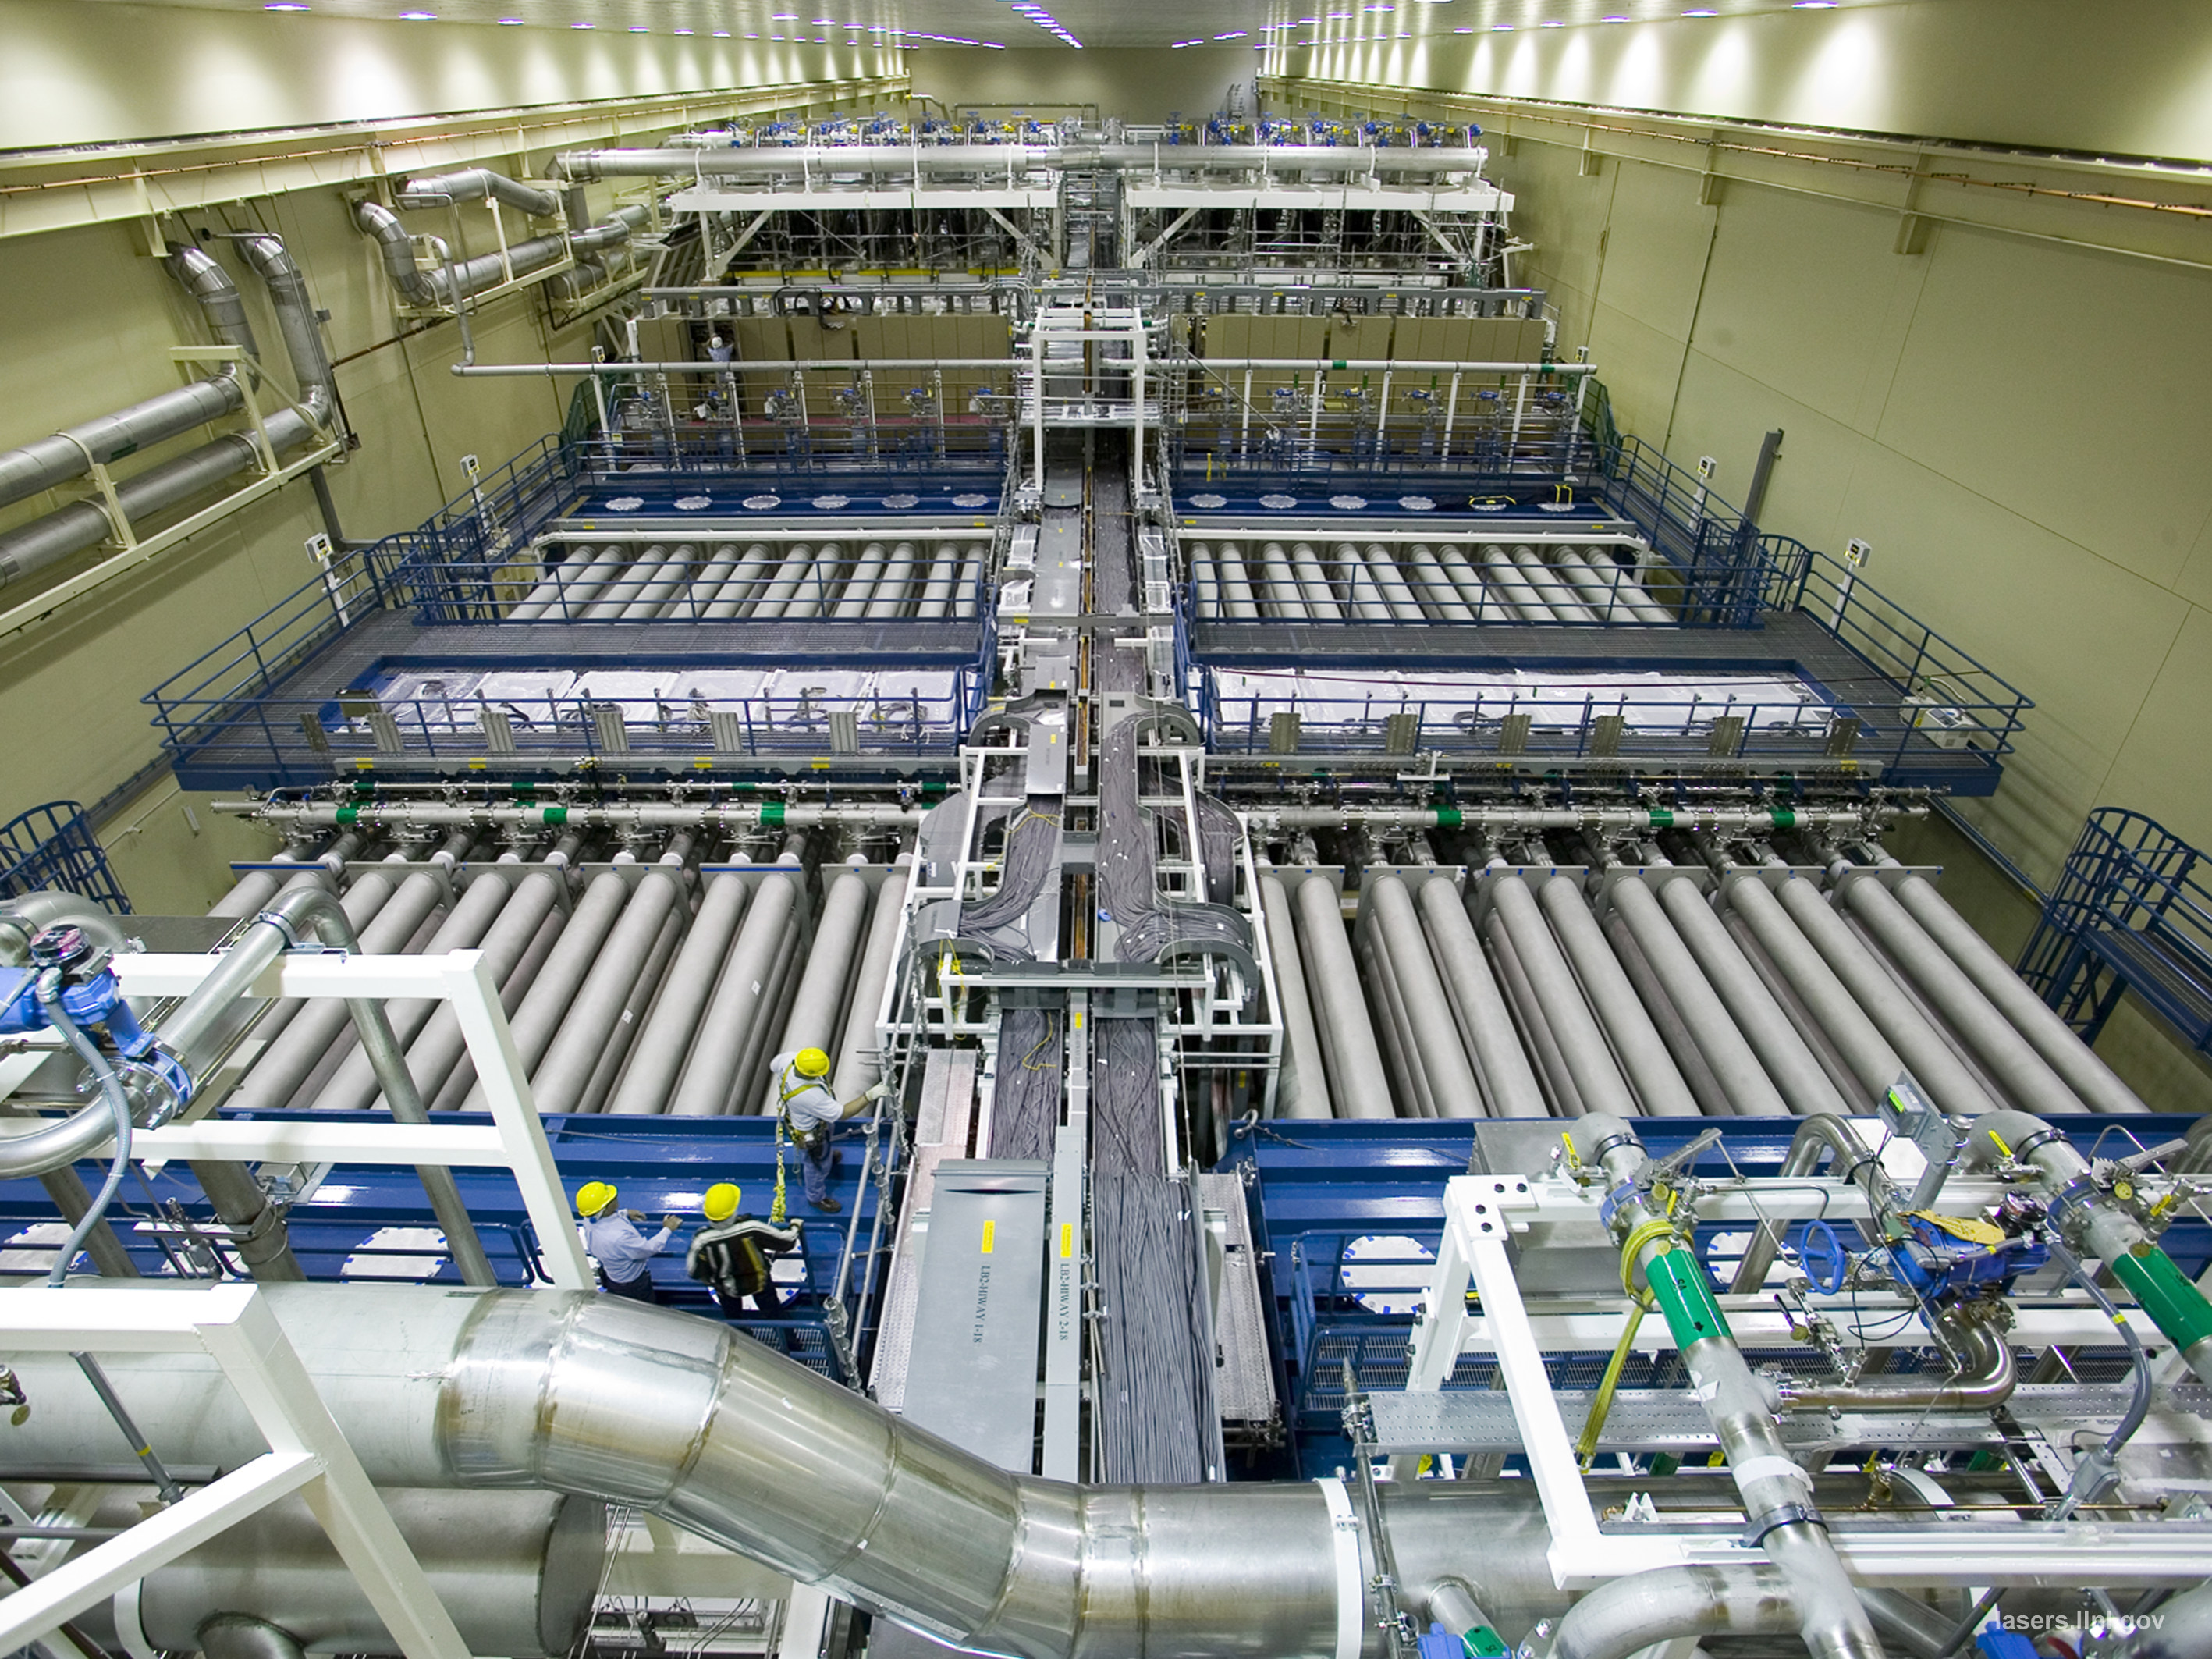
\includegraphics[width=90truemm]{slike/07_NIF_Laser_Bay.jpg}
\caption{Eden najmočnejših laserskih sistemov na svetu, ki doseže 
$500~\si{\tera\watt}$ moči v sunku. \\Vir: National Ignition Facility, Livermore, Kalifornija.}
\label{fig:NIF}
\end{figure}

Najmočnejši laserski sistemi oddajajo svetlobo z zelo veliko izhodno močjo. 
Najmočnejši zvezno delujoči laserji dosegajo moči 
$\sim 100~\si{\kilo\watt}$. Še bistveno večje moči dosegajo sunkovni laserji, 
saj lahko v sunku dosežejo moč tudi $\sim 500~\si{\tera\watt}$ (slika~\ref{fig:NIF}). 
Vendar so sunki s tako veliko svetlobno močjo izredno kratki, tipično reda pikosekunde, tako da
znaša celotna energija v sunku do nekaj $\si{\mega\joule}$. Pomemben
parameter pri sunkovnih laserjih je tudi čas, ki poteče med dvema zaporednima
sunkoma (repeticija). Najmočnejši laserski sistemi lahko izsevajo največ nekaj sunkov 
dnevno.\footnote{S. N. Dixit et al. CLEO: 2013, San Jose, CA (2013).}

\section{He-Ne laser}
\index{Laser!He-Ne}
Najprej si oglejmo helij-neon (He-Ne) laser, ki je bil prvi zvezno 
delujoči laser in je še danes zelo razširjen.\footnote{A. Javan, W. R. Bennet Jr. in 
D. R. Herriott, Phys. Rev. Lett. $\mathbf{6}$, 106 (1961).} Najpogosteje deluje 
pri valovni dolžini $632,8~\si{\nano\metre}$ v rdečem delu spektra, lahko 
pa tudi pri infrardečih $1,15~\si{\micro\metre}$ in 
$3,39~\si{\micro\metre}$ ter nekaterih drugih\index{Infrardeče valovanje}
valovnih dolžinah v oranžnem in zelenem delu spektra. Laser deluje v zveznem 
načinu delovanja s tipičnimi močmi $0,5$--$100~\si{\milli\watt}$.

Ojačevalno sredstvo je plin, mešanica helija in neona, katerih relevantni
energijski nivoji so prikazani na sliki~\ref{fig:HeNeE}. 
\index{Energijski nivoji!He-Ne}
\index{Trinivojski sistem}
Atome helija
s trki z elektroni vzbudimo v eno izmed dveh dolgoživih metastabilnih stanj $2^3S$ ali
$2^1S$ z razpadnima časoma $0,1~\si{\milli\second}$ in $5~\si{\micro\second}$.
Ti dve stanji slučajno praktično sovpadata z dvema stanjema neona ($4s$ in $5s$). 
Ko heliju dodamo neon, se energija s trki 
prenese z vzbujenih helijevih atomov na atome neona, ki s tem preidejo v 
že omenjeni vzbujeni stanji. Helijevi atomi se po trku vrnejo v osnovno stanje, od koder
jih ponovno vzbudimo. Prenos energije z atomov helija na atome neona s trki je 
zelo učinkovit, zato zasedenost vzbujenih neonovih stanj hitro naraste. Ko preseže 
zasedenost nižjih vzbujenih stanj, dosežemo obrnjeno zasedenost. 

\begin{figure}[h]
\centering
\def\svgwidth{100truemm} 
\input{slike/07_HeNeE.pdf_tex}
\caption{Shema energijskih nivojev v He-Ne laserju. Nivoji helija so označeni
z modro in nivoji neona z zeleno, laserski prehodi pa z rdečimi barvami in pripisano
ustrezno valovno dolžino.}
\label{fig:HeNeE}
\end{figure}

Znana rdeča svetloba He-Ne laserja z valovno dolžino $632,8~\si{\nano\metre}$ nastane 
pri prehodu iz stanja $5s$ v eno od stanj $3p$. Pri tem je življenjski čas 
stanja $5s$ okoli $100~\si{\nano\second}$, stanja $3p$ pa okoli $10~\si{\nano\second}$, zato
se spodnji nivo s spontano emisijo hitro prazni v metastabilno stanje $3s$. 
V tem stanju se atomi kopičijo, saj so dipolni sevalni prehodi v osnovno stanje prepovedani.
Atomi prehajajo v osnovno stanje le s trki ob steno cevi. Da pospešimo
praznjenje nivoja $3s$ in omogočimo večjo obrnjeno zasedenost, zmanjšamo 
premer razelektritvene cevi. Zaradi gibanja atomov je spektralna 
črta Dopplerjevo razširjena\index{Dopplerjeva razširitev} ($\Delta \nu = 1,5~\si{GHz}$). 

Laser deluje tudi pri prehodu iz $5s$ v stanje $4p$, pri katerem 
ima izsevana svetloba valovno dolžino $3,39~\si{\micro\metre}$. 
Ojačenje je za ta prehod celo precej večje kot za
prehod pri $632,8~\si{\nano\metre}$, deloma zaradi nižje frekvence 
(glej zvezo med Einsteinovima koeficientoma $A$ in $B$, enačba~\ref{4.27}), 
deloma zaradi kratke življenjske dobe spodnjega laserskega nivoja $4p$. 
Zato bi pričakovali, da bo He-Ne laser svetil v infrardečem delu in ne vidnem. 
To delno prepreči absorpcija v steklu, delno pa izgube namerno povečamo s selektivno odbojnostjo
resonatorskih zrcal, ki dvigne prag delovanja za $3,39~\si{\micro\metre}$ 
nad prag za $632,8~\si{\nano\metre}$. V laser lahko dodamo tudi
celico metana, ki infrardeč del svetlobe močno absorbira, vidnega pa ne.
Omenimo še prehode iz stanja $4s$, ki ga dosežejo neonovi atomi s trki
z vzbujenimi helijevimi atomi iz nivoja $2^3S$. Prehod $4s$ v $3p$, ki da svetlobo
pri $1,15~\si{\micro\metre}$, je bil prvi opažen prehod v He-Ne laserjih.
Zaradi razcepov posameznih nivojev je možnih prehodov še veliko več.

Tipičen He-Ne laser je razmeroma preprosto zgrajen (sliki~\ref{fig:HeNeShema}
in \ref{fig:Iskra}).\index{Laser!zgradba}
V razelektritveni cevi (napetost  $\sim 1~\si{\kilo\volt}$), skozi
katero teče električni tok ($\sim 10~\si{\milli\ampere}$), 
se nahaja mešanica helija in neona v razmerju od
$5:1$ do $10:1$. Skupni tlak v cevi je nizek, le okoli $3~\si{\milli\bar}$, 
cev pa je tipično dolga okoli $0,5~\si{\metre}$ s premerom $1$--$2~\si{\milli\metre}$.  
Cev s plinom na obeh straneh zapirata okni, ki sta nagnjeni za Brewstrov kot, 
tako da so izgube pri odboju za eno polarizacijo kar se da majhne.\index{Brewstrovo okno}
Izhodna svetloba iz laserja je zato polarizirana. V manjših laserjih
so namesto Brewstrovih oken na razelektritveno cev privarjena kar
resonatorska zrcala, zaradi česar so taki laserji nepolarizirani. 
Navadno je razelektritvena cev obdana z dvema ukrivljenima zrcaloma, 
ki imata zelo veliko odbojnost za izbrano valovno dolžino.
Nekaj tipičnih podatkov za He-Ne laser je zbranih v tabeli~(\ref{tab:Ar}).
\begin{figure}[h]
\centering
\def\svgwidth{100truemm} 
\input{slike/07_HeNeShema.pdf_tex}
\caption{Shema He-Ne laserja: R -- razelektritvena cev, IZ -- izhodno zrcalo, Z -- zrcalo
z veliko odbojnostjo, B -- Brewstrovi okni}
\label{fig:HeNeShema}
\end{figure}

\begin{figure}[h]
\centering
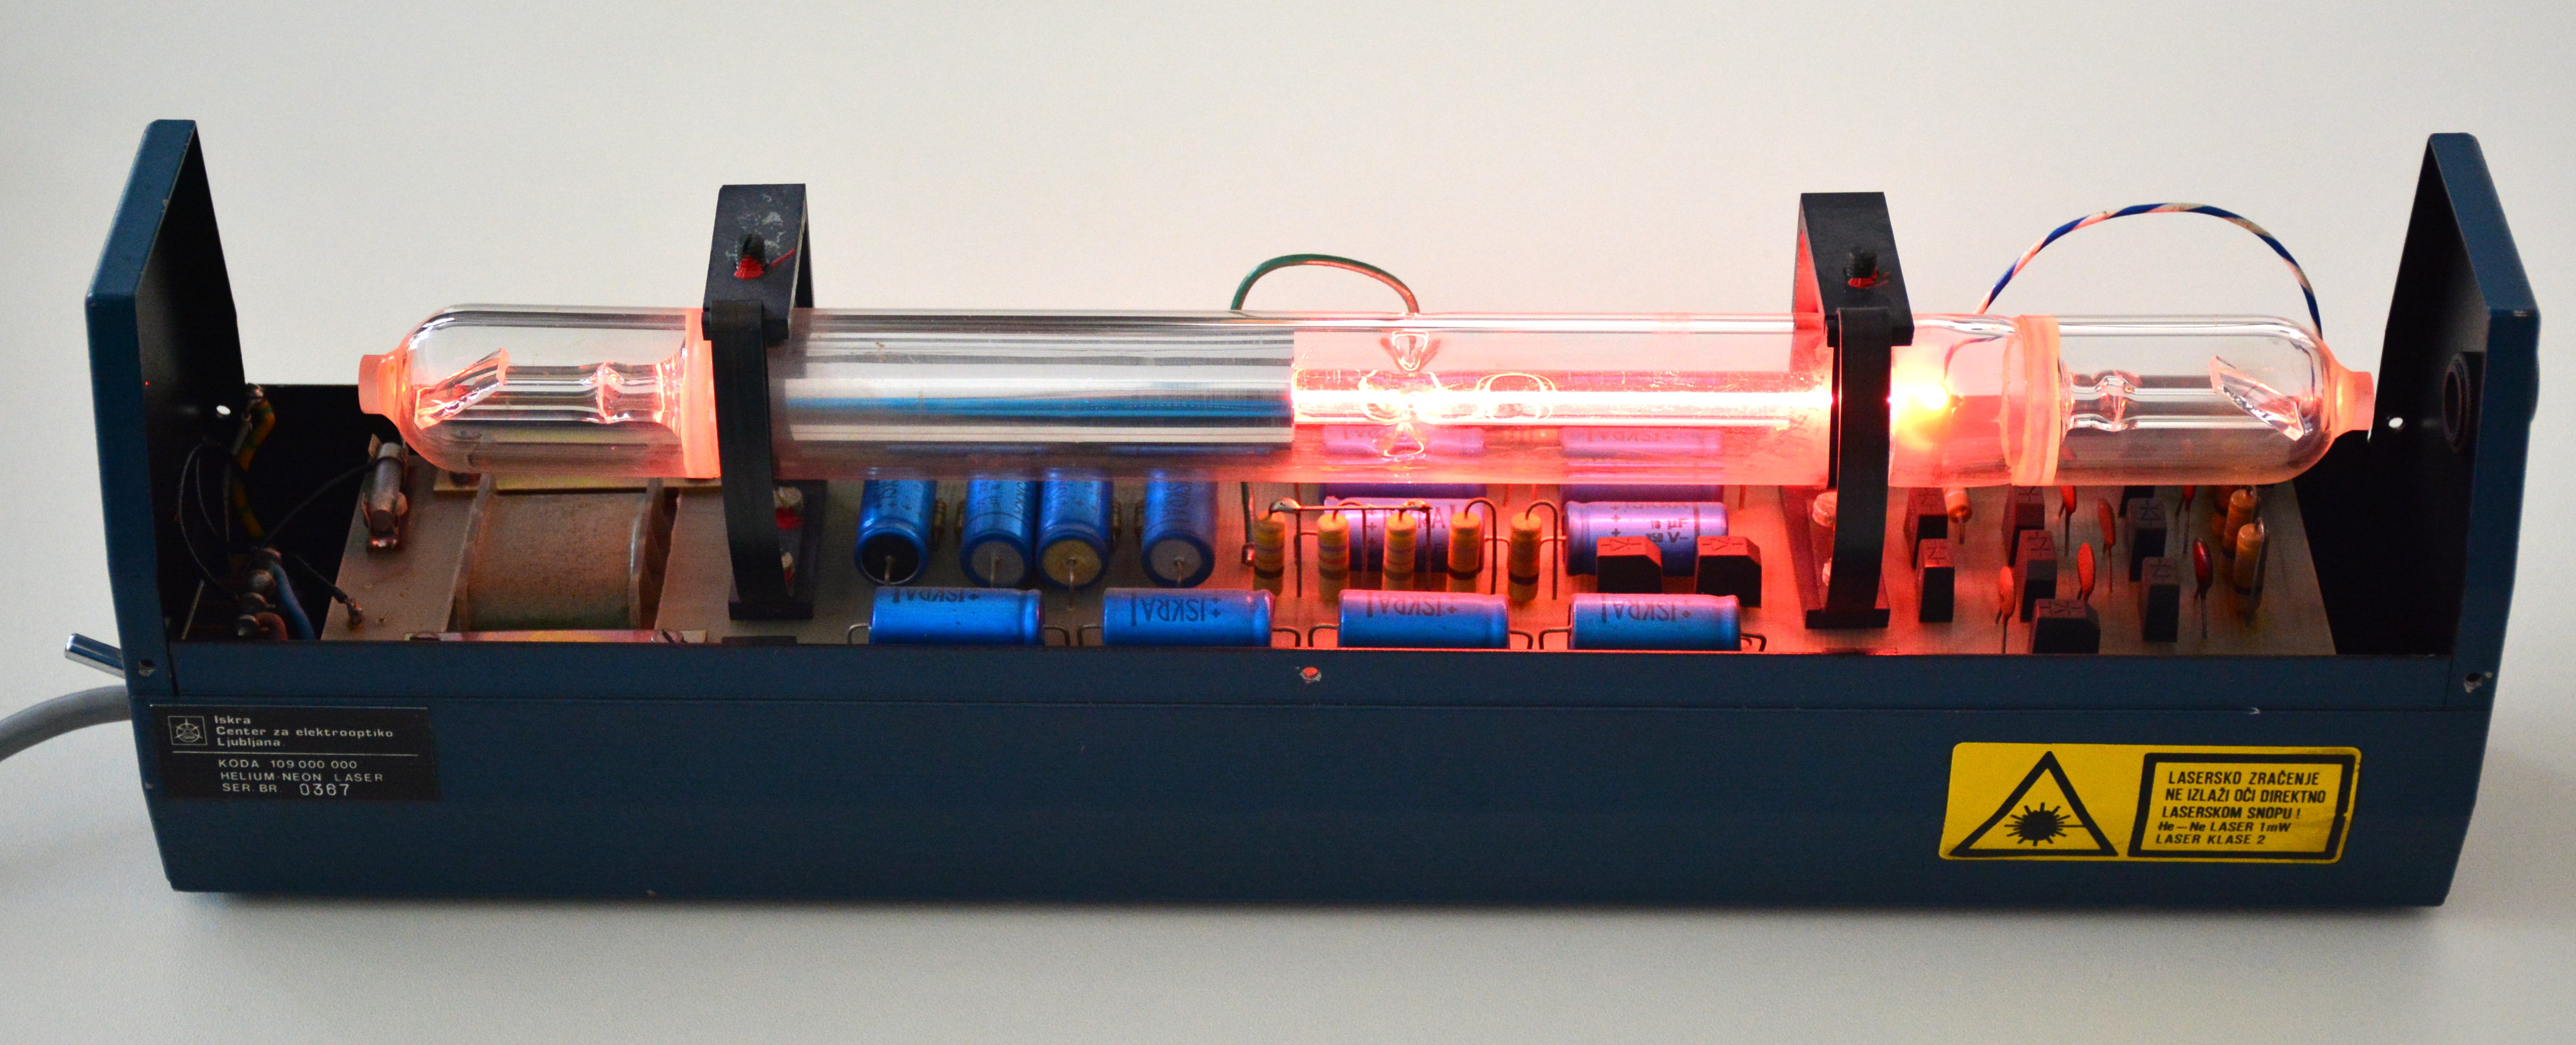
\includegraphics[width=100truemm]{slike/07_HeNe.jpg}
\caption{Primer starejšega He-Ne laserja, izdelanega v Sloveniji}
\label{fig:Iskra}
\end{figure}

He-Ne laserji so preprosti, stabilni, zanesljivi, poceni, imajo visoko kvaliteto snopa
in dolgo služijo ($\sim~50 000$ ur).
Danes jih sicer izrivajo polprevodniški laserji, vendar so še vedno v uporabi
v merilnih napravah, v optičnih bralnih sistemih, v šolah, v raziskovalnih 
laboratorijih za interferometrijo, holografijo itd. Na njem je osnovan tudi 
standard za meter.

\section{Argonov ionski laser}
\index{Laser!argonov}
Kot drugi primer plinskega laserja obravnavajmo argonov ionski (Ar$^+$) laser,
za katerega je značilno zvezno delovanje v modrem in zelenem delu spektra pri 
valovnih dolžinah $488,0~\si{\nano\metre}$ in $514,5~\si{\nano\metre}$, deluje 
pa tudi v bližnjem ultravijoličnem delu spektra. \footnote{W. B. Bridges,
Appl. Phys. Lett. $\mathbf{4}$, 128 (1964).} Tipične moči delovanja argonovega laserja
so od $100~\si{\milli\watt}$ do $50~\si{\watt}$.\index{Ultravijolično valovanje}

Kot večino plinskih laserjev tudi tega črpamo z električnim tokom.
Atome argona vzbudimo s trki z elektroni v ione argona, ti pa z nadaljnjimi
trki preidejo v vzbujena stanja. Obrnjeno zasedenost
dosežemo med nivojema $4p$ in $4s$ (slika~\ref{fig:ArE}). 
Ta dva nivoja vsebujeta veliko podnivojev, zato je tudi prehodov med
njima zelo veliko. Argonov laser tako seva pri več kot tridesetih različnih
valovnih dolžinah, najznačilnejši sta že omenjeni 488~nm in 514,5~nm. 
Življenjski čas zgornjega nivoja je okoli $10~\si{ns}$, kar je približno 
desetkrat več od življenjskega časa spodnjega nivoja, od koder se ioni
z rekombinacijo z elektroni vrnejo v osnovno stanje. Tudi pri tem laserju
je poglavitni vzrok za razširitev črte \index{Dopplerjeva razširitev}Dopplerjev 
pojav ($\Delta \nu = 3,5~\si{GHz}$).\index{Energijski nivoji!argon}

\begin{figure}[h]
\centering
\def\svgwidth{80truemm} 
\input{slike/07_ArE.pdf_tex}
\caption{Shema energijskih nivojev v Ar$^+$ laserju}
\label{fig:ArE}
\end{figure}

Argonov laser je v osnovi zgrajen podobno kot He-Ne laser. \index{Laser!zgradba}
V razelektritveni cevi
(tipična dolžina $1~\si{\metre}$ in premer $1$--$2~\si{\milli\metre}$)
se nahaja argon pri pritisku okoli $10~\si{\milli\bar}$. Ker gre pri 
vzbujanju atomov argona za dvostopenjski proces, mora biti električni tok, 
s katerim dosežemo obrnjeno zasedenost, precej velik, lahko tudi nekaj deset amperov. 
Pri tipični napetosti nekaj kV to pomeni, da so za delovanje potrebne velike električne moči, 
pogosto več deset $\si{\kilo\watt}$, in močnejši argonovi laserji morajo biti
zaradi velike količine odvečne toplote hlajeni, najpogosteje vodno.

\begin{figure}[h]
\centering
\def\svgwidth{100truemm} 
\input{slike/07_ArShema.pdf_tex}
\caption{Poenostavljena shema Ar$^+$ laserja s prizmo: R -- razelektritvena cev, 
IZ -- izhodno zrcalo, Z -- zrcalo z veliko odbojnostjo, B -- Brewstrovi okni, \index{Brewstrovo okno}
P -- prizma
}
\label{fig:ArS}
\end{figure}

\begin{remark}
V argonovih laserjih pogosto ustvarimo vzdolžno magnetno polje, ki preprečuje 
elektronom, da bi predčasno zapustili ojačevalno območje in trčili ob steno. S
tem se poveča izhodno moč laserja, hkrati pa preprečuje poškodbe na stenah, ki bi jih 
povzročili visokoenergijski elektroni. Iz istega razloga so pri močnejših
laserjih zrcala izven plinske cevi. 
\end{remark}

V resonator argonovega laserja moramo vgraditi še element, ki omogoči
izbiro ene same spektralne črte. Najpogosteje za ta frekvenčno selektiven element
uporabimo kar majhno prizmo pred enim od obeh zrcal (slika~\ref{fig:ArS}). Zaradi disperzije
v prizmi se snopi različnih valovnih dolžin lomijo pod različnimi koti in le tisti 
snop, ki vpada pravokotno na zrcalo, se ojačuje. Tako z vrtenjem prizme ali zrcala 
izbiramo valovno dolžino izhodne svetlobe. Nekaj tipičnih podatkov za argonov
laser je zbranih v tabeli~(\ref{tab:Ar}).

Argonovi laserji so zanesljivi in dajejo zelo dober osnovni Gaussov snop pri eni
sami frekvenci. Uporabljajo se v optični spektroskopiji,
interferometriji, holografiji in merilni tehniki. Delujejo v zveznem načinu,
zaradi razmeroma široke črte ojačenja jih uporabljamo tudi za fazno uklenjene
sunkovne laserje z dolžino sunkov okoli $150~\si{\pico\second}$. 
V kombinaciji s kriptonovimi laserji, ki so zelo podobni argonovim, le da delujejo
v rdečem in oranžnem delu spektra, se uporabljajo tudi v zabavni industriji.
V zadnjem času jih vse bolj izrivajo polprevodniški laserji in frekvenčno
podvojeni Nd:YAG. 

\section{CO$_\mathsf{2}$ laser}
\index{Laser!CO$_2$}
Do zdaj opisani plinski laserji delujejo na elektronskih prehodih v atomih oziroma ionih. 
Laser na ogljikov dioksid deluje na prehode med vibracijskimi stanji molekul 
CO$_2$, pri čemer elektroni ostanejo v osnovnem stanju.\footnote{C. K. N. Patel,
Phys. Rev. $\mathbf{136}$, A1187 (1964).}
Zaradi majhnih energijskih razlik med vibracijskimi stanji deluje
ta laser v infrardečem delu spektra, najpogosteje pri \index{Infrardeče valovanje}
$9,6~\si{\micro\metre}$ in $10,6~\si{\micro\metre}$. Laser deluje v zveznem
in v sunkovnem načinu. Odlikuje ga zelo velik izkoristek ($~\sim 30~\%$) in 
posledično zelo velike moči, tipično od $1~\si{\watt}$ do $10~\si{\kilo\watt}$. 

Preden opišemo delovanje laserja, si na kratko oglejmo lastna nihanja molekule 
ogljikovega dioksida. Molekula CO$_2$ je v osnovnem stanju linearna molekula 
(slika~\ref{fig:CO2}\,a). 
Za molekule take oblike obstajajo trije osnovni načini nihanja atomov glede na težišče:
atomi nihajo v smeri pravokotno na os (upogib, slika~\ref{fig:CO2}\,b),
atoma kisika nihata simetrično vzdolž osi molekule, ogljik pa pri tem miruje
(simetrični razteg, slika~\ref{fig:CO2}\,c) in atoma kisika nihata v isti smeri 
vzdolž osi, ogljik pa v nasprotni (asimetrični razteg, slika~\ref{fig:CO2}\,d). 
Pri tem ima najvišjo frekvenco asimetrični razteg in najnižjo upogib. 
Vsako vibracijsko stanje molekule lahko razstavimo na osnovne nihajne načine in 
ga opišemo s številom energijskih kvantov v posameznem osnovnem nihanju, 
torej s trojico celih števil $(n_1,n_2,n_3)$. Po dogovoru stanje 100 opisuje
osnovni simetrični razteg, stanje 010 osnovni upogib in stanje 001 
osnovni asimetrični razteg.

\begin{figure}[h]
\centering
\def\svgwidth{100truemm} 
\input{slike/07_CO2.pdf_tex}
\caption{Molekula CO$_2$ (a) in trije osnovni načini nihanja molekule:
upogib (b), simetrični razteg (c) in asimetrični razteg (d). Atom ogljika je označen s črno
in kisika z rdečo barvo.}
\label{fig:CO2}
\end{figure}

Vibracijska stanja molekule vzbudimo z električnim tokom skozi plin. 
\index{Energijski nivoji!CO$_2$}
Zato v razelektritveno cev dodamo dušik (N$_2$) in podobno kot pri He-Ne laserju
se tudi CO$_2$ črpa predvsem preko trkov z dušikovimi molekulami. 
Dušikova molekula je dvoatomna in ima zato zgolj eno vibracijsko stanje, ki po energiji
praktično sovpada z energijo stanja 001 (slika~\ref{fig:CO2E}). Iz tega zgornjega
nivoja molekule prehajajo v stanje 100 ($10,6~\si{\micro\metre}$) ali v stanje
020 ($9,6~\si{\micro\metre}$). Da pospešimo prehod nazaj v osnovno stanje, 
plinski mešanici dodamo helij, s katerim trkajo molekule.
Razmerje parcialnih tlakov je navadno 1:1:8 za CO$_2$:N$_2$:He pri tlaku $1~\si{\milli\bar}$. 
Pri tako nizkih tlakih je poglavitna razširitev spektralne črte Dopplerjeva, 
\index{Dopplerjeva razširitev}ki 
je v primerjavi z ostalimi plinskimi laserji zaradi nizkih frekvenc zelo majhna,
le okoli $70~\si{\mega\hertz}$. V laserjih z višjim tlakom 
prevlada razširitev zaradi medmolekulskih trkov. Pri tlakih okoli $20~\si{\bar}$
znaša razširitev okoli $500~\si{\giga\hertz}$, kar omogoča izdelavo fazno uklenjenih 
sunkovnih laserjev s sunki dolžine $\sim 1~\si{\pico\second}$. Nekaj tipičnih podatkov 
za laser na ogljikov dioksid je zbranih v tabeli~(\ref{tab:Ar}).

\begin{figure}[h]
\centering
\def\svgwidth{95truemm} 
\input{slike/07_CO2E.pdf_tex}
\caption{Shema vibracijskih nivojev v CO$_2$ laserju. 
Nivoji dušika so označeni z modro in nivoji CO$_2$ z zeleno, laserski prehodi 
pa z rdečimi barvami in pripisano ustrezno valovno dolžino.}
\label{fig:CO2E}
\end{figure}

Najpreprostejši laser na ogljikov dioksid \index{Laser!zgradba} 
je po svoji zgradbi podoben drugim plinskim laserjem. 
Razelektritvena cev (polmer $\sim 1~\si{\centi\metre}$ in dolžina $0,5$--$2~\si{\metre}$) 
je na obeh koncih zaključena z Brewstrovima oknoma in zrcaloma. Vsi optični elementi
v laserju morajo biti seveda prepustni oziroma odbojni za infrardeč del spektra. Ker lahko 
laser deluje pri različnih valovnih dolžinah, dodamo v resonator frekvenčno selektiven
člen, na primer uklonsko mrežico (slika~\ref{fig:CO2S}).\index{Uklonska mrežica}

\begin{figure}[h]
\centering
\def\svgwidth{100truemm} 
\input{slike/07_CO2Shema.pdf_tex}
\caption{Poenostavljena shema  CO$_2$ laserja: R -- razelektritvena cev, 
IZ -- izhodno zrcalo, Z -- zrcalo z veliko odbojnostjo, B -- Brewstrovi okni, 
U -- uklonska mrežica\index{Brewstrovo okno}
}
\label{fig:CO2S}
\end{figure}

Laserji na ogljikov dioksid se zaradi svoje velike moči uporabljajo v 
industriji za zahtevne obdelave materialov, na primer za rezanje 
kovin, vrtanje, ablacijo, varjenje in tudi za vojaške namene. Zaradi velike
absorpcije izsevane svetlobe v vodi se uporablja tudi v medicinske namene, predvsem
za rezanje tkiv in dermatologijo. 
Obdelava z laserji omogoča veliko natančnost, čistočo in je zelo fleksibilna.

\begin{table}
\small
\begin{center}
\begin{tabular}{|l|c|c|c|c|}\hline
Laser & He-Ne & Ar$^+$ & CO$_2$ & ekscimer\\ \hline
Valovna dolžina  $\lambda$ & $632,8~\si{\nano\metre}$& $488$ in
$514,5~\si{\nano\metre}$ & $9,6$ in $10,6~\si{\micro\metre}$ & UV
\\ \hline
Verjetnost za spontani prehod $A$ & $3,4 \times 10^6/\si{\second}$ & 
$7,8 \times 10^7/\si{\second}$ & $0,25/\si{\second}$ & $\sim 10^8/\si{\second}$ \\ \hline
Presek za stimulirano emisijo $\sigma$ & $3 \times 10^{-17}~\si{\metre}^2$&  $2,6 \times 10^{-16}~\si{\metre}^2$ & $3 \times 10^{-22}~\si{\metre}^2$ & $ 10^{-20}~\si{\metre}^2$ \\ \hline
Spektralna širina črte $\Delta \nu$ & $1,5 \times 10^{9}~\si{\hertz}$ & 
$3,5 \times 10^{9}~\si{\hertz}$ &$7 \times 10^{7}~\si{\hertz}$ & $10^{13}~\si{\hertz}$ \\ \hline
Obrnjena zasedenost $\Delta N/V$ & $5 \times 10^{15}/\si{\metre}^3$ & $2 \times 10^{15}/\si{\metre}^3$ & $3 \times 10^{21}/\si{\metre}^3$ & $10^{20}/\si{\metre}^3$\\ \hline
\end{tabular}
\caption{Izbrani podatki za He-Ne, Ar$^+$, CO$_2$ in tipičen ekscimerni laser}
\index{Laser!He-Ne}
\index{Laser!argonov}
\index{Laser!CO$_2$}
\index{Laser!ekscimerni}
\label{tab:Ar}
\end{center}
\end{table}

\section{Ekscimerni laser}
\index{Laser!ekscimerni}
Ekscimerji ({\it excited dimer, excimer}) so vzbujena vezana stanja dveh atomov, 
ki bi se v osnovnem stanju ne vezala.\footnote{N. G. Basov et al., JETP Lett.
$\mathbf{12}$, 329 (1970).}
Za laserje so zanimivi predvsem ekscimerji
težkih žlahtnih plinov in halogenov, na primer Ar$_2^*$ ($126~\si{\nano\metre}$), 
Kr$_2^*$ ($146~\si{\nano\metre}$), Xe$_2^*$ ($172~\si{\nano\metre}$),
ArF ($193~\si{\nano\metre}$), KrF ($248~\si{\nano\metre}$), 
XeCl ($308~\si{\nano\metre}$), ArBr ($161~\si{\nano\metre}$) in 
NeF ($108~\si{\nano\metre}$). Te molekule obstajajo samo v vzbujenem stanju,
v osnovnem stanju  je zaradi prevelike odbojne sile med atomoma molekula neobstojna.
Vsi našteti primeri oddajajo lasersko svetlobo v\index{Ultravijolično valovanje}
ultravijoličnem delu, ki ga drugi laserski sistemi le težko pokrivajo. 
Ekscimerni laserji delujejo v sunkih, pri čemer je tipična oddana energija v sunku 
$\sim 1~\si{\joule}$, dolžina sunka pa $10$--$100~\si{\nano\second}$ pri repeticiji
$\sim 100~\si{\hertz}$.

Dva atoma se vežeta, kadar je ionizacijska energija prvega
atoma manjša od vsote elektronske afinitete drugega atoma in
elektrostatične energije vezave obeh ionov. Vzemimo za primer klor in
kripton. Ionizacijska energija kriptona v osnovnem stanju je 14~eV, v
vzbujenem pa 5~eV. Elektronska afiniteta klora je 3,75~eV in
elektrostatična vezavna energija KrCl okoli 7~eV. Tako je treba za nastanek
molekule KrCl v osnovnem stanju dodati okoli 4~eV, pri tvorbi
molekule v vzbujenem stanju pa se sprosti okoli 6~eV. Odvisnost
potencialne energije molekule KrCl v osnovnem in vzbujenem stanju
kaže slika~\ref{fig:exE}. Molekula, ki je vezana v vzbujenem stanju, po
sevalnem prehodu v osnovno stanje takoj razpade, zato je zelo lahko doseči
obrnjeno zasedenost. Razpadni čas vezanega stanja je $\sim~10~\si{\nano\second}$ in
spodnjega nevezanega okoli $0,1~\si{\pico\second}$.
Da nastanejo ekscimeri, vzbujamo mešanico 
plinov v heliju. Pritisk
je razmeroma velik ($\sim 3~\si{\bar}$), zato plin v cevi vzbujamo prečno.
Velika je tudi spektralna širina prehoda ($\Delta\nu = 10^{13}~\si{Hz}$). Nekaj tipičnih podatkov 
za ekscimerne laserje je zbranih v tabeli~(\ref{tab:Ar}).
\index{Energijski nivoji!ekscimer}

Ekscimerni laserji delujejo v sunkih s precej veliko energijo in se zaradi kratke valovne
dolžine in velike natančnosti uporabljajo v fotolitografiji in izdelavi mikroprocesorjev 
ter v medicini, predvsem oftalmologiji in kirurgiji.
\vskip-3truemm
\begin{figure}[h]
\centering
\def\svgwidth{50truemm} 
\input{slike/07_exE.pdf_tex}
\caption{Shema energije v odvisnosti od razdalje med jedroma atomov. V vzbujenem stanju
se atoma povežeta v molekulo, po prehodu v nižji nivo  molekula razpade.}
\label{fig:exE}
\end{figure}

\section{Neodimov laser}
Druga skupina laserjev, ki jo bomo obravnavali, so trdninski laserji. Taki laserji
temeljijo na elektronskih prehodih v ionih primesi, ki jih dodamo v kristal ali steklo,
črpamo pa jih optično. Primesi so navadno redke zemlje ali prehodne kovine, 
kristali pa so oksidi ali fluoridi. Izdelava ojačevalnih sredstev na osnovi stekla
je bistveno bolj preprosta in poceni, vendar ima steklo precej nižjo toplotno prevodnost
od kristalov in se zato bolj greje. 
Začeli bomo z opisom dveh primerov neodimovega laserja, Nd:YAG
in Nd:steklo.\footnote{
Podobne laserje dobimo, če v kristalu YAG itrijeve ione deloma
nadomestimo z iterbijem ($1030~\si{\nano\metre}$) ali 
erbijem ($2940~\si{\nano\metre}$).\index{Iterbij}\index{Erbij}} 

\subsection{Nd:YAG}
\index{Laser!Nd:YAG}
V Nd:YAG laserju\footnote{J. E. Geusic,
H. M. Marcos in L. G. Van Uitert, Appl. Phys. Lett. $\mathbf{4}$, 182 (1964).} je ojačevalno sredstvo
itrij-aluminijev granat (Y$_3$Al$_5$O$_{12}$, YAG) s primesmi neodimovih ionov Nd$^{3+}$. 
Laser deluje pri valovni dolžini $1,064~\si{\micro\meter}$ ali frekvenčno podvojeni
$532~\si{\nano\metre}$. Deluje v zveznem \index{Infrardeče valovanje}
načinu pri močeh do $5~\si{\kilo\watt}$ ali sunkovnem z dolžino sunkov okoli 
$100~\si{\nano\second}$ in energijo sunka $\sim 1~\si{\joule}$.

Neodimov laser je primer štirinivojskega laserskega sistema, 
\index{Štirinivojski sistem}pri čemer je 
laserski prehod med stanjema $^4$F$_{3/2}$ in $^4$I$_{11/2}$ neodimovih ionov 
(slika~\ref{fig:NdE}). S svetlobo višje frekvence 
(tipično okoli $800~\si{\nano\metre}$) črpamo elektrone v višje nivoje, ki hitro 
preidejo v zgornji laserski nivo. Življenjski čas zgornjega nivoja je 
okoli $230~\si{\micro\second}$, spodnjega pa precej krajši, zato je 
lahko doseči veliko obrnjeno zasedenost. Spodnje stanje je dovolj visoko nad 
osnovnim, da pri sobni temperaturi v ravnovesju ni znatno zasedeno. 
Razširitev črte je homogena in je posledica predvsem \index{Spektralna črta!homogena razširitev}
termičnega nihanja kristalne mreže ($\Delta \nu = 130~\si{GHz}$). 
Prag neodimovega laserja za zvezno delovanje je nizek in ga je lahko doseči, 
prav tako dobro neodimov laser deluje v sunkih, predvsem s preklopom dobrote.
\index{Energijski nivoji!Nd:YAG}
\begin{figure}[h]
\centering
\def\svgwidth{85truemm} 
\input{slike/07_NdE.pdf_tex}
\caption{Shema energijskih nivojev neodimovih ionov v Nd:YAG laserju}
\label{fig:NdE}
\end{figure}

Laser optično črpamo z diodnimi laserji ali močnimi ksenonovimi svetilkami za zvezno delovanje 
ter podobnimi bliskavicami za sunkovno delovanje (slika~\ref{fig:Nd}\,a). 
Aktivna snov v laserju je v obliki paličice dolžine od nekaj cm do dobrih 
$10~\si{\centi\metre}$ in premera $\sim 1~\si{\centi\metre}$. 
V kristalu YAG neodimovi ioni nadomestijo približno $1~\%$ itrijevih, zato je ojačevalno
sredstvo na videz rahlo rožnato (slika~\ref{fig:Nd}\,b). 
Aktivna paličica in svetilka sta vgrajeni v cilindrično ali eliptično votlino z 
zrcalnimi ali belimi stenami, tako da se čim večji del črpalne svetlobe absorbira v 
laserski paličici (slika~\ref{fig:Nd}\,c).

\begin{figure}[h]
\centering
\def\svgwidth{120truemm} 
\input{slike/07_Nd.pdf_tex}
\caption{Ksenonova bliskavica (a), ojačevalno sredstvo v Nd:YAG laserju (b) 
in shema prečnega preseka eliptične črpalne votline (c)}
\label{fig:Nd}
\end{figure}

Pri črpanju s ksenonovo svetilko je le manjši del črpalne svetlobe v
absorpcijskih pasovih, zato je izkoristek razmeroma slab, tipično 
pod $1~\%$. Za izhodno moč zvezno delujočega Nd:YAG laserja $\sim 10~\si{\watt}$ je tako
potrebna električna moč $\sim \si{kW}$. Velika večina porabljene moči 
gre v gretje, zato je v laserjih z nekoliko večjo povprečno
močjo potrebno vodno hlajenje. Gretje povzroča tudi toplotne deformacije
laserske paličice, kar lahko močno spremeni lastnosti resonatorja. Toplotni
učinki so ena poglavitnih praktičnih težav pri izdelavi neodimovih
laserjev s klasičnimi svetilkami. Danes zato zvezno delujoče neodimove laserje
črpamo z diodnimi laserji, ki svetijo v območju največje
absorpcije Nd$^{3+}$. Črpanje je lahko prečno ali vzdolžno (slika~\ref{fig:NdS}). 
Pri diodnem črpanju je izkoristek dosti večji in je manj gretja, kar omogoča 
bolj kompaktno konstrukcijo in boljšo stabilnost izhodne moči.
\index{Laser!zgradba} 
\begin{figure}[h]
\centering
\def\svgwidth{120truemm} 
\input{slike/07_NdS.pdf_tex}\index{Črpanje!vzdolžno}
\caption{Shema vzdolžno črpanega Nd:YAG laserja. O -- ojačevalno sredstvo, 
IZ -- izhodno zrcalo, D -- dikroično zrcalo, 
prepustno za črpalno svetlobo in odbojno za lasersko, DL -- diodni 
laser za črpanje, L -- leča
}
\label{fig:NdS}
\end{figure}

Neodimovi laserji so zelo razširjeni, tako v osnovni kot tudi v frekvenčno 
podvojeni različici. Uporabni so za obdelavo materialov (vrtanje, varjenje, 
litografija). Ker snop preprosto sklopimo v optično vlakno, so 
zelo uporabni tudi v medicini (endoskopska kirurgija in dermatologija). 
Pomemben proizvajalec sunkovnih Nd:YAG laserjev 
za medicinske namene je podjetje Fotona d.o.o. iz Ljubljane.\index{Fotona d.o.o.}

\begin{table}[h]
\small
\begin{center}
\begin{tabular}{|l|c|c|c|}\hline
Laser & Nd:YAG & Nd:steklo & Ti:safir \\ \hline
Valovna dolžina  & $1064~\si{\nano\metre}$ & $1050~\si{\nano\metre}$ & 
 $600-1100~\si{\nano\metre}$\\ \hline
Verjetnost za spontani prehod $A$ & $4 \times 10^3/\si{\second}$ & $3 \times 10^3/\si{\second}$
& $3 \times 10^5/\si{\second}$\\ \hline
Presek za stimulirano emisijo $\sigma$ & $3 \times 10^{-23}~\si{\metre}^2$ &
$3 \times 10^{-24}~\si{\metre}^2$ & $3 \times 10^{-23}~\si{\metre}^2$\\ \hline
Spektralna širina črte $\Delta \nu$ & $1,3 \times 10^{11}~\si{\hertz}$ &
$7 \times 10^{12}~\si{\hertz}$ & $1 \times 10^{14}~\si{\hertz}$\\ \hline
Gostota obrnjene zasedenosti $\Delta N/V$ & $1,6 \times 10^{23}/\si{\metre}^3$ &
$8 \times 10^{23}/\si{\metre}^3$ & $6 \times 10^{23}/\si{\metre}^3$\\ \hline
\end{tabular}
\caption{Tipični podatki za Nd:YAG, Nd:steklo in Ti:safirni laser}
\index{Laser!Nd:YAG}
\index{Laser!Nd:steklo}
\index{Laser!Ti:safir}
\label{tab:nd}
\end{center}
\end{table}

\subsection{Nd:steklo}
\index{Laser!Nd:steklo}
Namesto v kristal lahko neodimove ione Nd$^{3+}$ vgradimo tudi v steklo. 
Laser z Nd:steklo ojačevalnim sredstvom deluje 
pri valovni dolžini $1,050~\si{\micro\meter}$ v sunkovnem načinu 
s preklopom dobrote ali z uklepanjem faz z energijami sunkov $~\sim 1~\si{\joule}$.
Zaradi amorfne strukture stekla in posledično 
nehomogenega lokalnega polja je laserska črta nehomogeno razširjena 
($\Delta \nu = 7~\si{THz}$).
\index{Spektralna črta!nehomogena razširitev}
Ojačenje je manjše kot v Nd:YAG in za prag laserskega delovanja je
potrebna precej večja črpalna moč. Laserji Nd:steklo se zato uporabljajo le v 
sunkovnem načinu in za tako delovanje so celo primernejši od Nd:YAG laserjev.
Zaradi manjšega ojačenja pri dani obrnjeni zasedenosti 
je v laserju s preklopom dobrote mogoče doseči večjo načrpanost preden pride do praznjenja
zaradi ojačevanja spontanega sevanja v enem preletu paličice. Problem teh laserjev
predstavlja nizka toplotna prevodnost stekla, ki omejuje repeticijo sunkov.
Velika širina spektralne črte je zelo primerna za delovanje v načinu uklepanja faz, s 
katerim dosegamo ultrakratke sunke ($\sim 100~\si{\femto\second}$). 

\begin{remark}
Energije izsevanih sunkov je mogoče še povečati z ojačevalniki. Med največjimi je
laserski sistem Nd:steklo, ki ga uporabljajo za raziskave fuzije (NIF - National Ignition Facility, 
Livermore, Kalifornija).
Okoli $1~\si{\nano\second}$ dolg sunek iz osnovnega laserja razdelijo na 192
ojačevalnih vej, sunek postopoma ojačujejo, nato ga na koncu spet združijo.
Končna energija sunka je tako nad $\sim 1~\si{\mega\joule}$. Z njim z vseh strani posvetijo na
kroglico iz devterija in tritija, ki se dovolj segreje in stisne, da pride do 
njunega zlivanja. Vršna moč laserskega sunka je okoli $10^{15}$~W. 
Če laserski snop zberemo na površino 1~mm$^2$, je v gorišču jakost električnega polja
okoli $5 \times 10^{11}$~V/m, kar je približno enako električnemu polju v vodikovem atomu.
\end{remark}

\section{Ti:safir laser}
\index{Laser!Ti:safir}
Titan-safirni laser je trdninski laser\footnote{P. F. Moulton, J. Opt. Soc. Am. B $\mathbf{3}$
125 (1986).}, pri katerem so v kristal safirja
Al$_2$O$_3$ primešani ioni titana Ti$^{3+}$. Njegova najpomembnejša značilnost je
zvezna nastavljivost valovne dolžine v zelo širokem frekvenčnem pasu 
($600$--$1100~\si{\nano\metre}$) z največjo učinkovitostjo pri okoli $800~\si{\nano\metre}$. Deluje
v zveznem načinu z močmi do $50~\si{\watt}$ in sunkovno  v fazno uklenjenem načinu 
z dolžino sunkov $\sim~10~\si{\femto\second}$ z vršnimi močmi nad $10^{12}~\si{\watt}$. 
\index{Energijski nivoji!Ti:safir}
\begin{figure}[h]
\centering
\def\svgwidth{90truemm} 
\input{slike/07_TiE.pdf_tex}
\caption{Energijski nivoji v Ti:safir laserju. Dva nivoja sta zaradi vibracij
razcepljena na veliko število podnivojev, ki se med seboj deloma prekrivajo.
Zelo podobna je tudi shema energijskih nivojev organskih barvil. 
}
\label{fig:TiE}
\end{figure} 

Ojačevalno sredstvo v Ti:safir laserju je aluminijev oksid, v katerem 
približno $0,2~\%$ aluminijevih ionov nadomestimo s titanovimi. Titanovi ioni imajo 
v taki konfiguraciji zgolj eno vzbujeno stanje, vendar se zaradi sklopitve s fononi
vibracijski nivoji posameznega stanja med seboj prekrivajo in prehod je močno razširjen. 
Z optičnim črpanjem vzbudimo titanove ione iz osnovnega stanja v eno izmed vibracijskih 
stanj vzbujenega stanja. Ioni nato hitro preidejo v najnižje vzbujeno stanje. 
Laserski prehod poteka med najnižjim vzbujenim stanjem in enim od vibracijskih 
nivojev osnovnega stanja (slika~\ref{fig:TiE}). Življenjski čas
vzbujenega stanja je kratek ($3,2~\si{\micro\second}$) in širina črte največja med
vsemi trdninskimi laserji ($\Delta \nu =  100~\si{THz}$). 
Ker je vrh absorpcijskega pasu blizu $500~\si{\nano\metre}$,
laser črpamo z zeleno svetlobo (argonov laser oziroma
frekvenčno podvojen neodimov laser za sunkovno delovanje). 
Najpomembnejša uporaba Ti:safir laserjev je v raziskovalnih laboratorijih za ustvarjanje zelo 
kratkih sunkov svetlobe z dolžino $\sim 10~\si{\femto\second}$. Pot, ki jo 
v tem času prepotuje svetloba, je le nekaj valovnih dolžin svetlobe. 

\section{Laserji na organska barvila}
\index{Laser!organska barvila}
Naslednja skupina laserjev so laserji na organska barvila, v katerih
je barvilo raztopljeno v tekočini, praviloma vodi ali alkoholu. 
To so bili prvi laserji z veliko spektralno širino in nastavljivo valovno dolžino
delovanja. Delujejo lahko kot zvezni laserji in z izbiro barvila dosežemo
delovanje v območju $300$--$1500~\si{\nano\metre}$ pri močeh do $\sim 2~\si{\watt}$.
Široka spektralna širina omogoča sunkovno delovanje z uklepanjem faz 
z nekaj femtosekundnimi sunki pri energiji sunka nekaj $100~\si{\joule}$.

Shema energijskih nivojev molekule tipičnega organskega barvila
je zelo podobna shemi energijskih nivojev Ti:safir laserja (slika~\ref{fig:TiE}).
Vsi elektronski nivoji so razcepljeni v vibracijske in rotacijske podnivoje. 
V toplotnem ravnovesju je molekula na dnu osnovnega elektronskega stanja S$_0$. 
Z absorpcijo vidne svetlobe primerne frekvence preide v neko vzbujeno
singletno stanje $S_1$. Preko trkov z molekulami topila vzbujena barvilna molekula
zelo hitro, v času okoli pikosekunde, preide na dno vzbujenega stanja, od
koder s sevanjem preide nekam v osnovno stanje $S_0$, od tam pa s trki
hitro nazaj na dno osnovnega stanja. Ker
sta obe elektronski stanji zaradi vibracij in rotacij razširjeni, sta 
absorpcijska in emisijska fluorescenčna črta široki ($\Delta \nu = 30~\si{THz}$).
Energija izsevane svetlobe je zmanjšana za energijo
prehodov s trki, zato je emisijska črta premaknjena k nižjim
frekvencam glede na absorpcijsko. Absorpcijski in fluorescenčni spekter prehoda $S_0-S_1$
za barvilo rodamin 6G kaže slika~\ref{fig:RhG}.
\vglue5truemm
\begin{figure}[h]
\centering
\def\svgwidth{80truemm} 
\input{slike/07_RhG.pdf_tex}
\caption{Absorpcijski in emisijski spekter barvila rodamin 6G, ki se uporablja v laserjih}
\label{fig:RhG}
\end{figure} 

\begin{table}[h]
\begin{center}
\begin{tabular}{|l|c|}\hline
Valovna dolžina  & $300$--$1500~\si{\nano\meter}$\\ \hline
Verjetnost za spontani prehod $A$ & $ \sim 10^8/\si{\second}$ \\ \hline
Presek za stimulirano emisijo $\sigma$ & $3 \times 10^{-20}~\si{\metre}^2$ \\ \hline
Spektralna širina črte $\Delta \nu$ & $3 \times 10^{13}~\si{\hertz}$  \\ \hline
Gostota obrnjene zasedenosti $\Delta N/V$ & $ \sim 10^{22}/\si{\metre}^3$ \\ \hline
\end{tabular}
\caption{Tipični podatki za laserje na organska barvila}
\label{tab:orgb}
\end{center}
\end{table}

Laser na organska barvila lahko deluje pri vseh frekvencah znotraj široke
fluorescenčne črte. Zato moramo v resonator vgraditi frekvenčno
selektivni element, s katerim nastavljamo frekvenco izhodne svetlobe. Za to lahko 
uporabimo prizmo ali eno od zrcal nadomestimo 
z uklonsko mrežico, ki je zasukana pod takim kotom, da se po osi resonatorja odbije le svetloba
izbrane valovne dolžine.\index{Uklonska mrežica}
Barvilne laserje črpamo ali z bliskavico ali z drugim laserjem primerne 
valovne dolžine, na primer argonovim ali ekscimernim laserjem. 

Slabost laserjev na organska barvila je njihova degradacija. Barvila v
laserjih je treba pogosto menjati (tipično na 100 ur delovanja), poleg tega je ravnanje
z njimi zahtevno, saj je veliko barvil in topil strupenih ali korozivnih.
Laserji na organska barvila so zaradi svoje nastavljive valovne dolžine
uporabni v spektroskopiji, za ločevanje izotopov, v 
medicini (dermatologija, odstranjevanje ledvičnih kamnov) ...
 
\section{Vlakenski laserji}
\index{Laser!vlakenski}
Posebna vrsta laserjev so vlakenski laserji, v katerih predstavlja aktivno 
sredstvo optično vlakno, dopirano z ioni \index{Optično vlakno}redkih zemelj.\footnote{Za
podroben opis optičnih vlaken glej poglavje~\ref{chap:fibri}.}
Valovna dolžina, pri kateri oddajajo svetlobo, je odvisna od snovi, s katerimi
je vlakno dopirano. Najpogosteje je to erbij ($1550~\si{nm}$),\index{Erbij}
iterbij ($\sim 1100~\si{nm}$)\index{Iterbij} ali neodim ($1064~\si{nm}$).
Vlakenske laserje odlikuje\index{Infrardeče valovanje}
izredno velik izkoristek (tipično okoli $70$--$80~\%$, lahko tudi več) 
in posledično zelo velika moč (do $20~\si{kW}$). Za njih sta značilni tudi
izredno velika kakovost snopa (faktor $M^2<1,1$, glej poglavje~\ref{chap:gaussovsnop}) in 
razmeroma majhna občutljivost na zunanje motnje. Delujejo lahko v zveznem
ali sunkovnem načinu.\index{Faktor $M^2$}

\begin{figure}[h]
\centering
\def\svgwidth{130truemm} 
\input{slike/07_FibEr.pdf_tex}
\caption{Energijski nivoji v erbijevem vlakenskem laserju (a) in 
absorpcijski ter emisijski spekter za erbij (b). Dodaten absorpcijski 
vrh pri $980~\si{nm}$ ni prikazan.}
\label{fig:ErFib}
\end{figure} 

Oglejmo si vlakenski laser, katerega vlakno je dopirano z ioni erbija 
(masni delež $\sim 1~\%$). Vlakna so pogosto dodatno dopirana z iterbijem, kar
poveča absorpcijo črpalne svetlobe in s tem izkoristek laserja. Laser črpamo
optično z lasersko diodo pri $980~\si{nm}$ ali $1480~\si{nm}$, laserski prehodi 
pa se zgodijo ob povratku v osnovno stanje. Osnovno stanje je razcepljeno v več podnivojev
(slika~\ref{fig:ErFib}), zato je valovna dolžina oddane svetlobe v razmeroma 
širokem intervalu $1520$--$1560~\si{nm}$. Velika spektralna širina
omogoča delovanje z uklepanjem faz. 

Zgradba vlakenskih laserjev se razlikuje od do zdaj opisanih. Glavna razlika je
seveda v resonatorju, ki je v tem primeru kar optično vlakno. Tipičen premer je 
$\sim 5~\si{\micro\meter}$ in dolžina več metrov. Na koncih vlakna lahko
postavimo dikroični zrcali, ki omogočata longitudinalno sklopitev črpalne svetlobe 
v vlakno. Namesto zrcal se pogosto uporablja periodične strukture 
na koncih vlakna, na katerih se valovanje izbrane valovne dolžine Braggovo odbija
(slika~\ref{fig:Fibshema}). \index{Laser!zgradba}\index{Braggov odboj}
S selektivnim odbojem se širina spektra izhodnega valovanja bistveno zmanjša. 

Navadno uporabljamo vlakna, ki so sestavljena iz sredice in dveh plaščev. Laserska
svetloba ostaja ujeta v sredici vlakna, medtem ko črpalno svetlobo vodimo po notranjem plašču. To
omogoča bistveno lažjo sklopitev črpalne svetlobe v vlakno. Poleg tega so zaradi povečanja
efektivnega polmera snopa vršne intenzitete manjše in posledično manjše verjetnosti
pojava neželenih nelinearnih pojavov (razdelek~\ref{NLOFIB}).

\begin{figure}[h]
\centering
\def\svgwidth{100truemm} 
\input{slike/07_Fibshema.pdf_tex}
\caption{Shema vlakenskega laserja: LD -- črpalna laserska dioda, 
BPS -- Braggova periodična struktura, V -- optično vlakno
}
\label{fig:Fibshema}
\end{figure}

Vlakenski laserji se uporabljajo v telekomunikacijah, saj oddajajo svetlobo 
valovnih dolžin, pri katerih je v vlaknih najmanjša disperzija (glej razdelek~\ref{chap:Disperzija}). 
Velika intenziteta svetlobe omogoča obdelavo materialov, varjenje, vrtanje in rezanje kovin. 
Zaradi svojih mehanskih lastnosti so primerni tudi za premično lasersko obdelavo snovi.

\begin{table}[!h]
\begin{center}
\begin{tabular}{|l|c|}\hline
Valovna dolžina  & $1550~\si{\nano\meter}$\\ \hline
Verjetnost za spontani prehod $A$ & $ \sim 90/\si{\second}$ \\ \hline
Presek za stimulirano emisijo $\sigma$ & $7 \times 10^{-25}~\si{\metre}^2$ \\ \hline
Spektralna širina črte $\Delta \nu$ & $3 \times 10^{12}~\si{\hertz}$  \\ \hline
Gostota obrnjene zasedenosti $\Delta N/V$ & $ \sim 10^{24}/\si{\metre}^3$ \\ \hline
\end{tabular}
\caption{Tipični podatki za erbijev vlakenski laser}
\label{tab:fib}
\end{center}
\end{table}

\begin{remark}
 Namesto vlaken, dopiranih z ioni redkih zemelj, lahko za izdelavo vlakenskih laserjev
 izkoristimo pojav stimuliranega Ramanovega sipanja (glej razdelek~\ref{chap:SRS}). 
 Pri tem pojavu se črpalna svetloba neelastično siplje, ojači pa se valovanje 
 pri nižji frekvenci. Razlika frekvenc ustreza vibracijskim prehodom 
 molekul, ki prevzamejo preostanek energije. Signal, ki se pri prehodu ojačuje, 
 ostaja pretežno ujet v vlakno z Braggovimi periodičnimi strukturami na koncih.
 Zavedati se moramo razlike med navadnim laserjem, ki deluje zaradi vzpostavljene
 obrnjene zasedenosti, in Ramanskim laserjem, v katerem se ojači sipana
 svetloba.\index{Laser!Ramanski}\index{Ramanovo sipanje!stimulirano}
\end{remark}

\section{Polprevodniški laserji}
\label{chap:SCL}
\index{Laser!polprevodniški}\index{Laser!diodni|see {Laser!polprevodniški}}
Danes so nedvomno najpomembnejši polprevodniški oziroma diodni 
laserji.
Njihove glavne značilnosti so veliko ojačenje in zato majhna 
dimenzija ($\sim 10$--$100~\si{\micro\metre}$), nizka cena, 
velik izkoristek ($\sim 50~\%$) in neposredno črpanje z električnim tokom. 
Za črpanje zadoščajo majhni tokovi \index{Črpanje}\index{Ultravijolično valovanje}
(tipično $\sim 100~\si{\milli\ampere}$), kar omogoča zelo hitro modulacijo (več $10~\si{GHz}$)
svetlobne moči s spreminjajočim se črpanjem. Slabost polprevodniških laserjev je razmeroma širok 
spekter in posledično majhna koherenca. Polprevodniški laserji delujejo v območju 
valovnih dolžin od $\sim 375~\si{nm}$ do več $\si{\micro\meter}$. Izhodne moči
so zelo odvisne od valovne dolžine: v UV območju so razmeroma nizke ($\sim 100~\si{mW}$),
sicer pa dosegajo vrednosti $\sim 3~\si{\watt}$.

Na hitro lahko rečemo, da delovanje diodnih laserjev temelji na rekombinaciji  
elektronov iz prevodnega pasu z vrzelmi v valenčnem pasu, pri čemer se izseva foton. Ta proces je lahko 
spontan, kot v svetlečih diodah, ali stimuliran, zaradi česar se svetloba ojači. 
Za podrobnejšo razlago ojačenja v polprevodniških 
laserjih moramo poznati osnove polprevodniške fizike, zato jo na kratko 
ponovimo.\footnote{Glej npr. N. W. Ashcroft in N. D. Mermin, {\it Solid State Physics}, Harcourt College
Publishers (1976).}

\subsection*{Energijski pasovi v polprevodnikih}
V trdnih snoveh elektroni niso lokalizirani in zaradi interakcij med sosednjimi atomi
se sicer ostra energijska stanja razširijo v energijske pasove. Zgornji pas je lahko 
le delno zaseden (kovine), lahko pa se med najvišjim polno zasedenim 
(valenčnim) pasom in najnižjim nezasedenim (prevodnim) pasom pojavi energijska reža. 
Če je velikost energijske reže $E_g$ nekaj $kT$, je snov polprevodnik 
(tabela~\ref{table:gap}), sicer je izolator.\index{Polprevodnik}
\begin{table}[h]
 \centering
\begin{tabular}{|l|c|c|c|c|c|c|} \hline  
      Snov & InSb & InAs & Ge & Si & GaAs & GaP \\ \hline
      $E_g~[\si{eV}]$ & 0,17 & 0,36 & 0,67 & 1,124 & 1,43 & 2,26  \\ \hline  
\end{tabular}
  \caption{Širina energijske reže $E_g$ v nekaterih polprevodnikih}
\label{table:gap}
\end{table}
\vglue-5truemm
Ko na polprevodnik vpade foton z energijo $\hslash\omega > E_g$, se foton absorbira, elektron
iz valenčnega pasu preide v prevodni pas in v valenčnem pasu ostane vrzel. Pričakovali bi, 
da se elektron, ki hitro preide na dno prevodnega pasu, spontano vrne v valenčni 
pas, pri čemer se svetloba izseva. Vendar je pri \index{Energijska reža}
prehodu treba upoštevati tudi ohranitev gibalne količine. Pri najobičajnejših polprevodnikih, 
siliciju in germaniju, leži vrh valenčnega pasu pri valovnem vektorju $\mathbf{k}=0$, 
dno prevodnega pasu pa pri $\mathbf{k} \neq 0$ (slika~\ref{fig:Ek}\,a).\index{Silicij}\index{Germanij}
\index{GaAs}\index{GaP}\index{InAs}\index{InSb}
Prehod elektrona preko take indirektne reže je malo verjeten, saj mora zaradi ohranitve 
gibalne količine priti še do interakcije s fononom. Prehod je veliko bolj verjeten v 
snoveh z direktno režo, pri katerih ležita tako dno prevodnega kot vrh valenčnega pasu 
pri $\mathbf{k}=0$ (slika~\ref{fig:Ek}\,b). Snovi z direktno režo so na primer GaAs in 
druge spojine elementov III. skupine (Al, Ga, In) in V. skupine (P, As, Sb), ki so najbolj 
uporabne za izdelavo diodnih laserjev.
\begin{figure}[h]
\centering
\def\svgwidth{145truemm} 
\input{slike/07_Ek.pdf_tex}
\caption{Energijski pasovi v polprevodniku, kjer modra označuje valenčni pas, 
zelena pa prevodnega. Reža je lahko indirektna (a) ali direktna (b). V vzbujenem stanju (c) so 
najnižja mesta v prevodnem pasu zasedena in najvišja mesta valenčnega pasu
izpraznjena. 
}
\label{fig:Ek}
\end{figure}

V najpreprostejši sliki obliko prevodnega pasu v bližini minimuma opišemo 
s parabolično odvisnostjo od velikosti valovnega vektorja $\mathbf{k}$
\beq
E_p = E_g + \frac{\hslash^2 k^2}{2m_p}.
\label{pp:Ec}
\eeq
Pri tem $m_p$ označuje efektivno maso elektrona v prevodnem pasu, ki upošteva
interakcije z mrežo in se zato razlikuje od mase prostega elektrona $m_0$.

Podobno z efektivno maso zapišemo energijo vrzeli v valenčnem pasu
\beq
E_v = - \frac{\hslash^2 k^2}{2m_v}.
\label{pp:Ev}
\eeq
Zapišemo še gostoti stanj na energijski interval za prevodni in valenčni pas. Izhajamo iz zveze
$\varrho(k) dk = k^2dk /\pi^2$ (enačba~\ref{4.3}) in z upoštevanjem 
enačb~(\ref{pp:Ec} in \ref{pp:Ev}) dobimo
\beq
\varrho_p(E) = \frac{1}{2\pi^2}\left(\frac{2m_p}{\hslash^2} \right)^{3/2} \sqrt{E-E_g}
\qquad \mathrm{in}\qquad
\varrho_v(E) = \frac{1}{2\pi^2}\left(\frac{2m_v}{\hslash^2} \right)^{3/2} \sqrt{-E}.
\label{eq:rho_p}
\eeq
Pri tem sta ključna parametra efektivna masa 
elektronov in vrzeli. Ti dve masi sta značilni za posamezen polprevodnik
in znašata v GaAs $m_p = 0,067~m_0$ in $m_v = 0,5~m_0$. 
Gostota stanj za vrzeli je v GaAs zato približno 
dvajsetkrat večja od gostote stanj za elektrone.\index{Gostota stanj}

Verjetnost za zasedenost stanj je podana s Fermi-Diracovo funkcijo 
\begin{equation}  
f_p(E)=\frac{1}{e^{(E-E_F)/k_B T}+1},
\label{eq:7FD}
\end{equation}
kjer $E_F$ označuje Fermijevo energijo. Pri $T=0$ so vsa stanja pod \index{Fermijeva energija}
Fermijevo energijo zasedena in nad njo prazna. Fermijeva energija leži
v energijski reži (slika~\ref{fig:Fermi}\,a). Pri končni temperaturi se na dnu prevodnega pasu nahajajo 
termično vzbujeni elektroni in na vrhu valenčnega pasu vrzeli (slika~\ref{fig:Fermi}\,b). Verjetnost 
za pojav vrzeli v valenčnem pasu je $f_v = 1 - f_p$.\index{Fermi-Diracova porazdelitev}
\begin{figure}[h]
\centering
\def\svgwidth{145truemm} 
\input{slike/07_Fermi.pdf_tex}
\caption{Verjetnost za zasedenost stanj. Pri $T=0$ je valenčni pas poln in prevodni prazen (a).
Pri končni temperaturi termično vzbujeni elektroni preidejo v prevodni pas (b). Za opis neravnovesnega
stanja uporabimo dve Fermijevi energiji $F_v$ in $F_p$, za vsak pas svojo (c).
}
\label{fig:Fermi}
\end{figure}
\vglue-0.5truecm
\begin{remark}
$E_F$ se določi iz pogoja, da je število elektronov v prevodnem pasu enako 
številu vrzeli v valenčnem pasu in $N_{p0} = N_{v0}$. Fermijeva energija
leži na sredini energijske reže le v primeru, da sta efektivni masi 
za elektrone in vrzeli enaki. Sicer se Fermijeva energija premakne
proti pasu z manjšo efektivno maso. 
\end{remark}

Število elektronov v prevodnem pasu na prostorninsko enoto izračunamo kot 
produkt gostote stanj in verjetnost, da je stanje zasedeno, integrirano po 
celotnem energijskem pasu
\beq
N_{p0}=\int_{E_g}^{\infty}\,\rho_p(E)f_p(E)\,dE.
\label{6.3a}
\eeq
Število vrzeli v valenčnem pasu je 
\beq
N_{v0}=\int_{-\infty}^{0}\,\rho_v(E)f_v(E)\,dE.
\label{6.3b}
\eeq
Število elektronov v prevodnem pasu (in vrzeli v valenčnem) je pri
$T=0$ enako nič in tudi pri končnih temperaturah ostaja razmeroma nizko. 
Znatno ga lahko povečamo, če polprevodnik dopiramo in s tem povišamo 
Fermijevo energijo.

Dopiranje polprevodnika pomeni nadzorovano dodajanje ustreznih nečistoč. 
Če dodamo donorske primesi, ki povečajo število elektronov v snovi, 
govorimo o polprevodniku tipa $n$. Če dodajamo akceptorske snovi, ki 
elektrone sprejemajo, govorimo o polprevodniku tipa $p$. \index{Polprevodnik!tip $n$}
Primeri donorjev za GaAs so žveplo, selen ali telur,\index{Polprevodnik!tip $p$}
primer akceptorjev pa cink in kadmij. 

Zaradi primesi se v energijski 
reži pojavi dodaten energijski nivo, pri čemer je donorski nivo navadno 
tik pod prevodnim pasom in akceptorski tik nad valenčnim. V polprevodniku tipa $n$ se
Fermijeva energija premakne navzgor, pri močnem dopiranju lahko tudi v 
prevodni pas. V tem primeru so zasedena vsa stanja v valenčnem pasu in vsa
stanja do Fermijeve energije v prevodnem. Podobno je v močno dopiranem polprevodniku tipa 
$p$, v katerem se Fermijeva energija pomakne navzdol in število vrzeli v valenčnem 
pasu močno naraste. Prosta so tako vsa stanja v prevodnem pasu in stanja do 
Fermijeve energije v valenčnem pasu.

\begin{remark}
 Zgolj z dopiranjem se verjetnost za prehod in izsevanje fotona ne spremeni. V
 polprevodniku tipa $n$, na primer, se število elektronov v prevodnem pasu sicer znatno poveča, 
 vendar v valenčnem pasu ni ustreznih vrzeli, s katerimi bi se elektroni rekombinirali.
\end{remark}

Ko elektrone vzbudimo iz valenčnega v prevodni pas, se v valenčnem pasu pojavijo
vrzeli. Dokler se ne rekombinirajo (tipično nekaj $\si{ns}$),
vlada v prevodnem pasu kvazi-termično ravnovesje, saj je relaksacija 
elektronov znotraj pasu bistveno hitrejša (tipično $\si{ps}$). 
Pri veliki populaciji elektronov v prevodnem in vrzeli v 
valenčnem pasu Fermijeva funkcija ni več dobra za opis zasedenosti stanj 
(sliki~\ref{fig:Ek}\,c in \ref{fig:Fermi}\,c). Uporabimo \index{Kvazi-Fermijeva energija}
koncept kvazi-Fermijevih nivojev $F_p$ in $F_v$, s katerima opišemo porazdelitvi
v vsakem pasu posebej, za prevodni in valenčni pas
\beq
f_p(E)=\frac{1}{e^{(E-F_p)/k_B T}+1} \qquad \mathrm{in} \qquad 
f_v(E)=\frac{1}{e^{(E-F_v)/k_B T}+1}.
\eeq
To lahko naredimo, ker je hitrost rekombinacije elektronov in vrzeli znatno počasnejša
od vzpostavljanja kvazi-ravnovesja znotraj pasu. V termičnem ravnovesju je razlika med 
kvazi-Fermijevima energijama $F_{p}-F_v$ enaka nič, z naraščajočim vzbujanjem pa se 
razlika povečuje.

\subsection*{Ojačenje svetlobe v polprevodnikih}
Posvetimo na polprevodnik v vzbujenem stanju s svetlobo s krožno frekvenco $\omega$.
Vpadna svetloba povzroča prehode med stanji z energijo $E_a$ v valenčnem 
in stanji z energijo $E_b$ v prevodnem pasu (slika~\ref{fig:Ek}\,b).
Če je prehodov iz prevodnega pasu v valenčnega več kot prehodov v obratni
smeri, se svetloba ojačuje.\index{Ojačenje v polprevodnikih}\footnote{Glej npr. 
B. E. A. Saleh in M. C. Teich, 
{\it Fundamentals of Photonics}, druga izdaja, John Wiley \& Sons, Inc. (2007).}

Za zapis verjetnosti za prehod med dvema stanjema na časovno
enoto uporabimo Fermijevo zlato pravilo. Verjetnost, da je zgornje stanje zasedeno, je 
$f_p(E_b)$, verjetnost za zasedenost spodnjega stanja pa je $1-f_v(E_a)$. Verjetnost 
za prehod pri določenem valovnem vektorju je\index{Fermijevo zlato pravilo}
\begin{equation}  
w_s(k)=\frac{2\pi}{\hslash}|H_{pv}|^2\delta(E_b-E_a- \hslash\omega)
f_p(E_b)[1-f_v(E_a)],
\label{6.5}
\end{equation}
kjer je $H_{pv}= \langle p| \hat{x}|v\rangle E $ matrični element za dipolni
prehod  med prevodnim in valenčnim pasom v svetlobnem polju $E$. Podobno je
verjetnost za absorpcijo 
\begin{equation}  
w_a(k)=\frac{2\pi}{\hslash}|H_{pv}|^2\delta(E_b-E_a- \hslash\omega)
f_v(E_a)[1-f_p(E_b)].
\label{6.6}
\end{equation}
Upoštevamo enačbi~(\ref{pp:Ec}) in (\ref{pp:Ev}) in zapišemo razliko energij
\begin{equation}  
E_b-E_a= E_g + \frac{\hslash^2 k^2}{2}(\frac{1}{m_p}+ \frac{1}{m_v})= E_g + \frac{\hslash^2 k^2}{2m_r},
\label{6.8}
\end{equation}
kjer smo z $m_r=m_v m_p/(m_v+m_p)$ označili reducirano maso elektrona in vrzeli.

Število emisij oziroma absorpcij na enoto volumna v danem času izračunamo tako,
da verjetnosti za prehod integriramo po vseh $\mathbf{k}$. Razliko med številom 
emisij in absorpcij na enoto volumna je
\begin{align}  
N_{pv}-N_{vp}&=\int\left(w_s-w_a\right)\rho(k)\,dk  \nonumber \\
&=\frac{2}{\pi\hslash} \int |H_{pv}|^2\left(f_p(E_b)-f_v(E_a)\right)
\delta \left(\frac{\hslash^2 k^2}{2m_r}+E_g -\hslash\omega\right) k^2\,dk.
\label{6.7}
\end{align}
Upoštevali smo, da je gostota stanj $\rho(k)=k^2\, dk/\pi^2$. Vpeljemo
novo spremenljivko 
\beq
X = \frac{\hslash^2 k^2}{2m_r}+E_g -\hslash\omega
\eeq
in zapišemo integral
\beq
N_{pv}-N_{vp}=\frac{1}{\pi\hslash}\left(\frac{2m_r}{\hslash^2}\right)^{3/2} 
\int |H_{pv}|^2 \left(f_p(E_b)-f_v(E_a)\right)
\sqrt{\left(X-E_g+\hslash \omega\right)}\,
\delta (X) dX.
\label{6.7a}
\eeq
Z upoštevanjem lastnosti funkcije $\delta$ zapišemo
\begin{equation}  
N_{pv}-N_{vp}=\frac{1}{\pi\hslash}\left(\frac{2m_r}{\hslash^2}\right)^{3/2}
|H_{pv}|^2 \sqrt{\hslash \omega-E_g}\left(f_p(E_b)-f_v(E_a)\right).
\label{6.11}
\end{equation}
Poglejmo rezultat podrobneje. Da je število prehodov iz prevodnega v valenčni pas
večje od števila prehodov v obratno smer in se torej vpadna svetloba ojačuje
namesto absorbira, mora biti $N_{pv}-N_{vp} >0$. Sledi pogoj
\begin{equation}  
\frac{1}{e^{(E_b-F_{p})/k_B T}+1}>\frac{1}{e^{(E_a-F_v)/k_B T}+1}.
\label{6.12}
\end{equation}
Upoštevamo zvezo $E_b-E_a = \hslash \omega$ in zahtevo, da mora biti število prehodov realno. 
Dobimo pogoj za ojačevanje 
\boxeq{6.13}{  
E_g \leq \hslash\omega<F_{p}-F_{v}.
}
Energija fotonov, ki se v snovi ojačujejo, mora biti po pričakovanjih večja od
energije reže, sicer se niti ne absorbirajo niti ne ojačujejo. Pogoj za ojačevanje pove tudi, 
da za ojačenje svetlobe ne zadošča le nekaj vzbujenih elektronov in nekaj ustreznih vrzeli. 
V prevodnem pasu mora biti toliko elektronov, da pri neki energiji zasedejo vsaj polovico stanj, 
hkrati  mora biti v valenčnem pasu toliko vrzeli, da je vsaj polovica stanj nezasedena.
Ojača se torej le svetloba z energijo fotonov, ki je manjša od razlike med kvazi-Fermijevima
nivojema. 

Koeficient ojačenja vpadne svetlobe pri dani krožni
frekvenci $\omega$ je
\beq
\gamma(\omega) = K \sqrt{\hslash \omega - E_g}\left(f_p(E_b)-f_v(E_a)\right),
\label{eq:gainSC}
\eeq
pri čemer smo konstante pospravili v sorazmernostni faktor $K$. Za ojačenje velja
\beq
dj = \gamma(\omega) j dz.
\eeq
Z naraščajočo stopnjo vzbujenosti 
koeficient ojačenja razumljivo narašča, manjša pa se z naraščajočo 
temperaturo. Njegovo odvisnost od energije vpadnih fotonov kaže slika~\ref{s6.11}. Vidimo,
da se z naraščajočo temperaturo zmanjšuje tudi širina pasu, v katerem se svetloba ojačuje.
\begin{figure}[h]
\centering
\def\svgwidth{80truemm} 
\input{slike/07_gamma.pdf_tex}
\caption{Ojačenje v polprevodniku kot funkcija energije vpadnih fotonov. Črna črta
velja pri $T=0$ in rdeča pri $T>0$. Pri frekvencah, večjih od $(F_p-F_v)/\hslash$,
se svetloba absorbira. 
}
\label{s6.11}
\end{figure}

\subsection*{Spoj $\textbf{\textit{p}}$-$\textbf{\textit{n}}$}
\index{Spoj $p$-$n$}
Svetloba se v polprevodniku ojačuje le, če je na istem mestu v prevodnem pasu
dovolj veliko število elektronov in v valenčnem pasu zadosti vrzeli. Za delovanje
polprevodniškega laserja moramo torej s črpanjem vzdrževati neravnovesno stanje, 
podobno kot smo pri navadnih laserjih vzdrževali obrnjeno zasedenost. 
Neravnovesno stanje dosežemo tako, da v degeneriran pol\-pre\-vod\-nik tipa $p$, v
katerem je veliko vrzeli, dovolj hitro dodajamo elektrone v prevodni pas. To lahko storimo s spojem
$p$-$n$, na katerega priključimo napetost v prevodni smeri. \index{Črpanje}

Najpreprostejši primer spoja $p$-$n$ je spoj dveh kosov iste snovi, ki je
na eni strani dopirana z akceptorji ($p$) in na drugi z donorji ($n$). 
Ko staknemo območji $p$ in $n$, elektroni iz območja z višjo koncentracijo 
difundirajo v območje z nižjo koncentracijo in vrzeli ravno obratno. 
Ob spoju nastane v stacionarnem stanju ozek pas, tako imenovani izpraznjeni sloj, 
v katerem ni prostih nosilcev naboja. Na strani $n$ ostanejo pozitivni donorski ioni in 
na strani $p$ negativni akceptorski ioni, ki ustvarjajo električno polje. 
Nastalo polje preprečuje nadaljnjo difuzijo nosilcev naboja. 
V ravnovesju se Fermijeva energija na obeh straneh izenači, 
prevodni in valenčni pas pa se ukrivita (slika~\ref{fig:pnlaser}\,a).
\begin{figure}[h]
\centering
\def\svgwidth{150truemm} 
\input{slike/07_pnlaser.pdf_tex}
\caption{Energijska pasova v močno dopiranem spoju $p$-$n$ (a) in 
ista pasova ob priključeni napetosti v prevodni smeri (b). $F_p$ in $F_v$
označujeta kvazi-Fermijevi energiji in senčen del  aktivno območje, 
v katerem se elektroni in vrzeli rekombinirajo.
}
\label{fig:pnlaser}
\end{figure}

Ko na spoj priključimo napetost v prevodni smeri (torej pozitivno napetost na stran
$p$), se potencialni skok zmanjša. Pri tem je potencialna razlika kar sorazmerna priključeni
napetosti $U$. Fermijevi energiji na $p$ in $n$ strani se razmakneta in v
ozkem območju v bližini spoja pride do hkratne zasedenosti elektronov
v prevodnem pasu in vrzeli v valenčnem pasu (slika~\ref{fig:pnlaser}\,b). 
\index{Spoj $p$-$n$!{aktivno območje}}
To imenujemo aktivno območje, saj v njem prihaja do rekombinacij in do nastanka fotonov. 

Pri nizkih 
priključenih napetostih oziroma nizkih tokovih skozi spoj $p$-$n$ prihaja
do spontane rekombinacije in nizke izsevane moči svetlobe. 
Pri večjih napetostih, ko je $e_0U \approx E_g$, so koncentracije nosilcev naboja velike in
stimulirane rekombinacije omogočajo optično ojačenje. Takrat presežemo prag delovanja
diodnega laserja. \index{Prag delovanja laserja}
Ojačenje v polprevodniških laserjih je precej veliko, lahko več od 
$100~/\si{cm}$, zato je mogoče dobiti delujoč laser že v zelo majhnem aktivnem 
območju, lahko tudi le nekaj mikronov. Navadni polprevodniški laserji so tako 
dolgi $\sim~0,25~\si{mm}$.

\subsection*{Zgradba laserja}
Prvi polprevodniški laser je bil narejen iz GaAs  in je oddajal svetlobo \index{GaAs}
pri $850~\si{nm}$\footnote{R. N. Hall 
et al., Phys. Rev. Lett. $\mathbf{9}$, 366 (1962).}. 
Shema takega laserja je na sliki~\ref{fig:pnshema}. Svetloba se v njem ojačuje
v tanki aktivni plasti in iz laserja izhaja v smeri vzdolžno z laserjem. 
Vidimo, da polprevodniški laser nima resonatorja iz dveh odbojnih zrcal,
ampak se svetloba odbija kar na gladko odklanih stranskih ploskvah kristala. Zaradi
velikega lomnega količnika (npr. $n=3,5$ za GaAs) je odbojnost dovolj velika
za učinkovito delovanje.\index{Laser!zgradba}
\begin{figure}[h]
\centering
\def\svgwidth{140truemm} 
\input{slike/07_pnshema.pdf_tex}
\caption{Shema preprostega polprevodniškega laserja (a) in porazdelitev svetlobne
intenzitete na spoju $p$-$n$. Tipična širina je $100$--$200~\si{\micro\metre}$, 
dolžina $200$--$500~\si{\micro\metre}$ in debelina aktivne plasti  $\sim 1~\si{\micro\metre}$. 
Svetlobni profil v laserju (b). Svetloba 
se ojači v aktivnem območju (vijolična). V območjih $p$ in $n$ se svetloba absorbira.
}
\label{fig:pnshema}
\end{figure}

Opisani polprevodniški laserji imajo kar nekaj slabosti. So zelo močno dopirani, 
dobro delujejo le močno hlajeni (prvotno pri $77~\si{K}$), poleg tega je snop 
v takih laserjih pogosto širši od debeline aktivnega območja. To znaša
$\sim 1~\si{\micro\meter}$, širina snopa pa nekaj mikronov več, zato
znaten del svetlobe potuje po območju $p$ in $n$, kjer se absorbira in posledično
snov segreva. Tokovi, potrebni za 
delovanje takega laserja, so visoki ($\sim 100~\si{kA}/\si{cm}^2$ pri sobni temperaturi) in
kakovost snopa razmeroma slaba. 

Bistveno izboljšano delovanje je v tako imenovanih 
heterostrukturah.\footnote{Za 
iznajdbo heterostruktur sta Zhores I. Alferov in Herbert Kroemer leta 2000 prejela Nobelovo nagrado.}
 To so dvojni spoji $p$-$n$, 
v katerem sta spojeni dve različni snovi, medtem ko se aktivno območje (tipično debelo le okoli $100~\si{nm}$) 
nahaja med polprevodnikoma tipa $p$ in $n$.\footnote{H. Kroemer, Proc. IEEE $\mathbf{51}$, 1782 (1963).}
Najpomembnejši primer je plast $p$-GaAs, ki se nahaja med plastjo  \index{Heterostruktura}
$n$-Al$_x$Ga$_{1-x}$As in $p$-Al$_x$Ga$_{1-x}$As \index{AlGaAs}
(slika~\ref{fig:hetero}\,a). Elektroni v tem primeru tečejo iz tipa $n$ v prevodni pas aktivne plasti
GaAs in vrzeli iz tipa $p$ v valenčni pas. 
Tak laser deluje v območju od $750~\si{nm}$ do $880~\si{nm}$, odvisno od $x$ in koncentracije primesi.
Drug pomemben primer je laser z In$_{x}$Ga$_{1-x}$As$_{1-y}$P$_y$, ki seva svetlobo z valovno 
dolžino med $1,1~\si{\micro\metre}$ in $1,6~\si{\micro\metre}$. To ga naredi še posebej pomembnega za optične
komunikacije, v katerih se najpogosteje uporablja svetlobo pri $1,3~\si{\micro\meter}$ in $1,55~\si{\micro\meter}$. 
Prvi primer si oglejmo podrobneje.\index{Infrardeče valovanje}
\begin{figure}[h]
\centering
\def\svgwidth{145truemm} 
\input{slike/07_hetero.pdf_tex}
\caption{Shema laserja z dvojno heterostrukturo (a) in oblika energijskih pasov 
na spoju pri napetosti, priključeni v prevodni smeri (b). V aktivnem območju
je število elektronov v prevodnem pasu in vrzeli v valenčnem pasu zelo veliko, zato se 
svetloba močno ojačuje.
}
\label{fig:hetero}
\end{figure}
\begin{remark}
Pri izdelavi heterostruktur je ključno najti snovi, ki imajo čim bolj podobno strukturo.
Take plastne strukture naredijo z epitaksialno rastjo, zato si morajo biti medatomske
razdalje različnih materialov čim bolj podobne. V nasprotnem primeru se pojavijo 
defekti, zaradi katerih naprava slabše deluje. 
GaAs in AlAs imata enako strukturo in praktično enako medatomsko razdaljo, zato 
lahko brez škode na strukturi atome galija zamenjamo z atomi aluminija. Tipične 
vrednosti $x$ v Al$_x$Ga$_{1-x}$As so $0,3$. S spreminjanjem koncentracije aluminija $x$ hkrati
zvezno spreminjamo širino energijske reže ($E_g \approx 1,42 + 1,3x~\si{eV}$) in lomni količnik 
zlitine ($n \approx 3,5-0,71x$).
\end{remark}

Heterostruktura ima nekaj poglavitnih prednosti. Zlitina z aluminijem ima večjo 
energijsko režo od čistega GaAs, zato mejni plasti ustvarita potencialno bariero, 
ki preprečuje difuzijo nosilcev naboja iz aktivne plasti (slika~\ref{fig:hetero}\,b). Tako ostane koncentracija 
elektronov v prevodnem pasu in vrzeli v valenčnem pasu že pri razmeroma majhnih tokovih
velika in svetloba se ojačuje. Druga prednost je manjši lomni količnik zlitine, 
zaradi katerega ostane svetloba ujeta v aktivni plasti, podobno kot v valovnem 
vodniku. Ker manjši del svetlobe potuje izven aktivnega območja, je ojačenje večje,
poleg tega se zaradi večje energijske reže občutno zmanjša absorpcija izven aktivnega območja.
Skupaj z zmanjšano debelino aktivnega območja to vodi do znižanja tokov, 
potrebnih za delovanje laserja, za približno dva reda velikosti ($\sim 1~\si{kA}/\si{cm}^2$). 
Z uporabo heterostrukture se tudi izboljša izkoristek in zmanjša gretje.  

Pri strukturi, ki jo kaže slika~\ref{fig:hetero}, je aktivna plast v prečni smeri praktično neomejena, 
zato lahko hkrati sveti mnogo nihanj. Posledično je prečna koherenca snopa razmeroma slaba in 
delovanje laserja nestabilno. To slabost popravijo z jedkanjem plasti ob straneh, da ostane le
kakih $5~\si{\micro\meter}$ širok pas (\ref{fig:heshema}). Odjedkani material nadomestijo s čistim Al$_x$Ga$_{1-x}$As, 
tako da je aktivno območje z vseh strani obdano s snovjo z večjim lomnim količnikom in laserski
snop ostane ujet v pravokoten valovni vodnik. Izhodni snop je zaradi oblike aktivne snovi eliptičen s 
premerom okoli $1~\si{\micro\meter}$ v navpični in $5~\si{\micro\meter}$ v prečni smeri. 
V večji oddaljenosti je divergenca snopa $\sim~50~\si{\degree}$ v navpični in $\sim~5~\si{\degree}$ 
v prečni smeri. Če potrebujemo cilindrično simetričen snop, ga moramo popraviti z ustreznimi 
lečami.
\begin{figure}[h]
\centering
\def\svgwidth{95truemm} 
\input{slike/07_heshema.pdf_tex}
\caption{Shema laserja z dvojno heterostrukuro z dodatno prečno omejitvijo
}
\label{fig:heshema}
\end{figure}

\begin{remark}
Omenili smo, da polprevodniški laserji nimajo posebnih zrcal. Zaradi velikega lomnega
količnika polprevodnika se dovolj svetlobe odbije na mejni ploskvi. Vendar naloga resonatorja ni 
samo odboj svetlobe, ampak tudi izbira posameznega nihajnega načina. Ker tega z odbojem 
na ploskvi ne dosežemo, pogosto uporabimo periodične strukture, na katerih se svetloba selektivno
Braggovo odbije. Druga možnost je periodično spreminjajoča se debelina plasti, na kateri pride
do porazdeljene povratne sklopitve ({\it distributed feedback}). \index{Braggov odboj}\index{Porazdeljena
povratna sklopitev}
 
Večja odbojnost mejnih ploskev je nujna v laserjih, pri katerih svetloba ne izhaja iz
tanke aktivne plasti vzporedno z ravnino spoja $p$-$n$, ampak izhaja v smeri pravokotno na aktivno plast.
To so tako imenovani VCSEL ({\it Vertical Cavity Surface-Emitting 
Laser}).\footnote{F. Koyama et al., Trans. IEICE ${\mathbf E71}$, 1089 (1988).} Ker je sevalna površina večja in 
ojačevalno sredstvo krajše, je ojačenje na prelet manjše in mora biti odbojnost resonatorja toliko večja. 
Kakovost snopa je v takih laserjih občutno boljša kot v navadnih diodnih laserjih, poleg tega ima izhodni 
snop manjšo divergenco.\index{Laser!VCSEL}
\end{remark}

\begin{remark}
Posebna vrsta polprevodniških laserjev so nizkodimenzionalni laserji. V njih je 
velikost aktivnega območja vsaj v eni smeri primerljiva z medatomsko razdaljo (tipično $\sim 10~\si{nm}$).
Najpreprostejši je laser s potencialno jamo ({\it quantum well laser}), \index{Laser!s potencialno jamo}ki 
je po svoji zgradbi zelo podoben heterostrukturnim (slika~\ref{fig:heshema}), le da so dimenzije precej
manjše. Zaradi majhne dimenzije se v taki snovi bistveno zmanjša gostota stanj. \index{Gostota stanj}
Za dosego zahtevane razlike med kvazi-Fermijevimi nivoji, s čemer dosežemo prag za delovanje laserja,
je zato potrebna precej manjša gostota nosilcev naboja in tok, potreben za delovanje laserja,
se zniža. 

Kvantne pike, ki sicer niso laserji, so kvantno omejene v vseh treh smereh.
V njih so stanja diskretna in pasov ni več. Ker je tehnološko zelo zahtevno izdelati povsem enake
kvantne pike, je spekter izsevane svetlobe iz skupine kvantnih pik zelo nehomogeno razširjen. 
\end{remark}

Diodni laserji so danes eni najpomembnejših laserjev. Uporabljamo jih v vsakodnevnih napravah 
(tiskalnikih, optičnih bralnikih), v medicini, industriji, izrednega
pomena so za telekomunikacije, pogosto jih uporabljamo tudi za 
črpanje trdninskih ali vlakenskih laserjev. 
Poleg že naštetih prednosti jih odlikuje tudi zelo dolg življenjski čas ($\sim~50 000$~ur). 

\subsection{Svetleče diode - LED}
\index{Svetleče diode}\index{LED|see {Svetleče diode}}
Svetleče diode so danes eden najbolj razširjenih izvorov svetlobe in nadomeščajo
navadne žarnice ali svetilke. Oddajajo svetlobo od UV do IR, odlikujeta jih \index{Ultravijolično valovanje}
dober izkoristek (nad $25~\%$) in dolga življenjska doba ($\sim~50 000$~ur).

Svetleče diode delujejo podobno kot polprevodniški laserji. Na spoju $p$-$n$ prihaja do 
spontane emisije fotonov zaradi rekombinacij elektronov in vrzeli. Za razliko od laserjev 
svetleče diode nimajo praga delovanja, ampak začnejo svetiti, čim je na spoj priključena 
napetost v prevodni smeri. Zaradi spontane narave prehodov je svetloba, ki jo oddajajo
svetleče diode, nekoherentna in nepolarizirana. \index{Spoj $p$-$n$}

Prve svetleče diode, ki so oddajale svetlobo v vidnem delu spektra,
so bile izdelane iz GaAsP\index{GaAsP} in so oddajale 
svetlobo pri $710~\si{nm}$.\footnote{N. Holonyak Jr. in S. F. Bevacqua, Appl. Phys. Lett.
${\mathbf 1}$, 82 (1962).} Pomemben
napredek je bila izdelava svetlečih diod, ki so oddajale svetlobo v modrem delu 
spektra.\footnote{Za iznajdbo modrih LED so Isamu Akasaki, Hiroshi Amano in 
Shuji Nakamura leta 2014 prejeli Nobelovo nagrado.} Te so sestavljene iz dvojne
heterostrukture, v kateri je plast InGaN, dopiranega s cinkom, 
med plastema $p$-AlGaN in $n$-AlGaN.

Belo svetlobo iz LED svetil lahko dobimo z mešanjem svetlobe iz treh različnih 
diod: rdeče, zelene in modre. Bolj primeren je pristop z uporabo ene same diode, 
ki oddaja svetlobo v modrem delu spektra. Tako diodo prevlečemo z molekulami fosforja, ki
modro svetlobo absorbira in spontano izseva svetlobo pri nižjih frekvencah 
oziroma daljših valovnih dolžinah. Z ustrezno izbiro parametrov dobimo belo svetlobo
ceneje in preprosteje kot s tremi ločenimi diodami. 

\begin{remark}
Posebna vrsta svetlečih diod so organske svetleče diode (OLED).\footnote{C. W. Tang in
S. A. VanSlyke, Appl. Phys. Lett. $\mathbf{51}$, 913 (1987).} Te so narejene iz
organskih snovi, ki se obnašajo kot organski polprevodniki. S spreminjanjem kemijske
sestave se spreminja valovno dolžino, ki jo LED oddaja. Njihova poglavitna prednost
je preprosta izdelava, saj je proizvodnja organski spojin preprostejša in cenejša
od rasti kristalov. \index{Svetleče diode!OLED}
\end{remark}

%Manjkajo Vlakenski in polprevodniški

%-------------------------------------------------------------------------------
%	CHAPTER 8
%-------------------------------------------------------------------------------

\chapterimage{Mavrica.jpg} % Chapter heading image

\chapter{Nelinearna optika}
\label{chap:NLO}
Pri obravnavi svetlobnega valovanja v snovi smo doslej vedno privzeli linearno 
zvezo med polarizacijo in jakostjo električnega polja. To 
je seveda približek, ki je dovolj dober le pri razmeroma majhnih jakostih
polja. Kadar doseže jakost polja velike vrednosti -- in v laserskih snopih
jih nedvomno lahko doseže -- je treba upoštevati tudi višje člene v razvoju. Takrat
govorimo o nelinearni optiki\index{Nelinearna optika}, saj zveza med polarizacijo
in električnim poljem ni linearna. V tem poglavju bomo spoznali zanimive pojave, ki jih 
povzroči nelinearni del polarizacije, med drugim optično 
podvajanje frekvenc, optično usmerjanje, samozbiranje laserskega snopa, 
optične solitone in optično fazno konjugacijo. 

\section{Nelinearna susceptibilnost}
\label{Chap:Chi}
V linearnem približku odziva snovi velja, da je polarizacija snovi\index{Električna polarizacija} 
$\mathbf{P}$ linearna funkcija električne poljske jakosti svetlobe 
$\mathbf{E}$\index{Električno polje!jakost}. Takrat zapišemo (enačba~\ref{eq:PM})
\beq
\mathbf{P} = \mathbf{D} - \varepsilon_0 \mathbf{E} = 
\varepsilon_0 \underline{\epsilon} \cdot\mathbf{E} - \varepsilon_0 \mathbf{E} = 
\varepsilon_0 (\underline{\epsilon} - 1)\cdot\mathbf{E}. 
\eeq
Če uvedemo tenzor linearne susceptibilnosti\index{Susceptibilnost!linearna}
\beq
\chi^{(1)} = \underline{\epsilon} - 1,
\eeq
lahko linearni odziv snovi zapišemo strnjeno kot
\beq
\mathbf{P}_{\mathrm{L}} =  \varepsilon_0 \chi^{(1)} \cdot \mathbf{E}.
\eeq
Ta približek je dober za majhne jakosti električnega polja. Pri večjih poljih
postanejo pomembni tudi členi višjega reda v razvoju polarizacije
po $\mathbf{E}$
\boxeq{8.1}{
\mathbf{P}=\mathbf{P}_{\mathrm{L}}+ \mathbf{P}_{\mathrm{NL}}=
\epsilon_{0} \chi^{(1)}\cdot \mathbf{E}+
\epsilon_{0}\chi^{(2)}:\mathbf{E}\, \mathbf{E}+
\epsilon_{0}\chi^{(3)}\vdots \mathbin \mathbf{E}\mathbin \mathbf{E}\mathbin\mathbf{E} + \dots
}
Vpeljali smo nelinearni susceptibilnosti\index{Susceptibilnost!nelinearna} 
$\chi^{(2)}$ in $\chi^{(3)}$, ki sta tenzorja tretjega in četrtega ranga. 
Za bolj nazorno predstavo izpišimo nelinearna dela še po komponentah
\beq
\left(\mathbf{P}_{\mathrm{NL,2}}\right)_i= \epsilon_{0}\chi^{(2)}_{ijk} \,E_j \,E_k
\label{eq:nlin2}
\eeq
in 
\beq
\left(\mathbf{P}_{\mathrm{NL,3}}\right)_i= \epsilon_{0}\chi^{(3)}_{ijkl} \,E_j \,E_k\, E_l,
\label{eq:nlin3}
\eeq
pri čemer smo uporabili Einsteinov zapis seštevanja po indeksih. Značilne vrednosti
susceptibilnosti v trdnih snoveh so $\chi^{(1)} \sim 1$, 
$\chi^{(2)} \sim 10^{-12}~\textrm{m/V}$ 
in $\chi^{(3)} \sim 10^{-22}$~m$^2$/V$^2$. Obravnavali bomo samo snovi, v katerih
ni izgub in so susceptibilnosti realne.

\begin{definition}
Pokaži, da so gostote svetlobnega toka, pri katerih dosežemo znaten nelinearen 
prispevek k polarizaciji 
 $$\frac{P_{NL}}{P_L} \sim 10^{-6},$$
velikostnega reda 1~MW/cm$^2$. 
Ker so take vrednosti z navadnim svetilom povsem nedosegljive, je bilo mogoče nelinearne
optične pojave opazovati šele po iznajdbi laserjev.
\end{definition}
 
Tenzor $\chi^{(2)}$ je od nič različen le v snoveh, ki nimajo centra inverzije. 
Ker lahko v produktu (enačba~\ref{eq:nlin2}) vrstni red $E_j E_k$ zamenjamo, mora biti
tenzor invarianten na to zamenjavo
\beq
\chi_{ijk} = \chi_{ikj}.
\label{eq:chijk}
\eeq
Vpeljemo poenostavljen zapis, pri katerem prvi indeks prepišemo $(x = 1, y = 2, z = 3)$,
zadnja dva indeksa pa združimo. Dogovorjene oznake so $xx = 1, yy = 2, zz = 3, yz = zy =4, 
xz = zx =5, xy = yx = 6$. Tako na primer $\chi_{xxz}$ zapišemo kot $\chi_{15}$. Namesto
splošnega tenzorja tretjega ranga smo torej uvedli matriko velikosti $3\times6$. 
Vendar koeficienti matrike niso poljubni. Zaradi simetrijskih lastnosti kristala se matrika
poenostavi in navadno je le nekaj komponent različnih od nič. 
Kadar je v snovi absorpcija pri vseh treh frekvencah dovolj majhna, lahko matriko poenostavimo
z dodatnim približkom, tako imenovano  
\index{Kleinmanova domneva} Kleinmanovo domnevo\footnote{D. A. Kleinman, Phys. Rev. 126, 1977 (1962).}.
Ta pravi, da je 
\beq
\chi_{ijk} = \chi_{ikj} = \chi_{kij} = \chi_{kji} = \chi_{jik} = \chi_{jki}.
\eeq
\begin{table}[h!]
 \centering
\begin{tabular}{|c|c|c|c|} \hline  
      Kristal & Grupa & Neničelne komponente tenzorja $\chi$ & Vrednosti ($10^{-12}$~m/V)\\ \hline
      BaTiO\index{BaTiO$_3$}$_3$ & 4mm & $\chi_{xxz} = \chi_{yyz} = \chi_{xzx} = \chi_{yzy} = 
      \chi_{15} = \chi_{24}$  &
	    $\chi_{15} = 42,6$ \\
	      & & $\chi_{zxx} = \chi_{zyy} = \chi_{31} = \chi_{32}$ &  $\chi_{31} = 45,2$ \\
	      & & $\chi_{zzz} = \chi_{33}$ & $\chi_{33} = 16,0$ \\ \hline
      KDP\index{KDP} & 
      $\overline{4}$2m & $\chi_{xyz} = \chi_{yxz} = \chi_{xzy} = \chi_{yzx} = \chi_{14} = \chi_{25}$  &
	    $\chi_{14} = 0,88$ \\
	    & & $\chi_{zxy} = \chi_{zyx} = \chi_{36}$ &  $\chi_{36} =1,12$ \\ \hline
      Telur\index{Telur} & 32 & $\chi_{xxx} = -\chi_{xyy} = -\chi_{yyx} = -\chi_{yxy} =$  & \\
      & &  = $\chi_{11} = -\chi_{12}=-\chi_{26}$  &
	    $\chi_{11} = 1300$ \\
	    & & $\chi_{xyz} = \chi_{xzy} = -\chi_{yxz}= - \chi_{yzx}= \chi_{14} = 
	    -\chi_{25}$ &  $\chi_{14} \approx 0$ 
	    \\ \hline
      LiNbO$_3$\index{LiNbO$_3$} & 3m & $\chi_{xxz} = \chi_{yyz} = \chi_{xzx} = \chi_{yzy} = \chi_{15} = \chi_{24}$  &
	    $\chi_{15} \approx \chi_{31}$ \\
	     & & $\chi_{zxx} = \chi_{zyy} = \chi_{31} = \chi_{32}$ &  $\chi_{31} = -11,9$ \\
	      & & $\chi_{zzz} = \chi_{33}$ & $\chi_{33} = 68,8$ \\
	    & &  $-\chi_{xxy} = - \chi_{xyx} = \chi_{yyy} = -\chi_{yxx}  = $ & \\
	    & & $=-\chi_{16} = \chi_{22}$ = $-\chi_{21}$  &
	    $\chi_{22}  = 5,52$ \\
\hline 
\end{tabular}
  \caption{Koeficienti nelinearne susceptibilnosti za nekaj izbranih snovi}
\label{table:chi}
\end{table}

Poglejmo primer. Vzemimo barijev titanat (BaTiO$_3$)\index{BaTiO$_3$} s točkovno grupo 4mm. To pomeni, da
ima 4-števno os simetrije in dve zrcalni ravnini, od katerih ena preslika $x \to -x$ ali $y \to -y$, 
druga pa $x\to y$ in $y\to x$. Od nič različni elementi susceptibilnosti so tako samo:
\beq
\chi_{xxz} = \chi_{xzx} =   \chi_{yyz} = \chi_{yzy}  ; \quad  \chi_{zzz}; \quad \chi_{zxx} = \chi_{zyy}.   
\eeq
Z upoštevanjem Kleinmanove domneve se število različnih členov še zmanjša in ostaneta le dva
\beq
\chi_{xxz} = \chi_{xzx} = \chi_{yyz} = \chi_{yzy} =\chi_{zxx} = \chi_{zyy} \quad \mathrm{in} \quad \chi_{zzz}.   
\eeq
V tabeli~(\ref{table:chi})\footnote{Izmerjene vrednosti, ki jih najdemo v literaturi, 
se med seboj pogosto znatno razlikujejo.} so navedene izmerjene vrednosti in vidimo, da Kleinmanova
domneva ni povsem točna, ampak zgolj dober približek. 

\section{Nelinearni optični pojavi drugega reda}
\index{Nelinearna optika!drugega reda}
Vzemimo optično nelinearni kristal s $\chi^{(2)} \neq 0$. V smeri pravokotno 
glede na njegovo mejno ploskev naj vpadata dve valovanji s frekvencama
$\omega_{1}$ in $\omega_{2}$. Zaradi nelinearne sklopitve nastajajo v snovi nova 
valovanja z različnimi kombinacijami frekvenc (glej sliko~\ref{fig:nl2}).
\begin{figure}[h]
\centering
\def\svgwidth{140truemm} 
\input{slike/08_nl3.pdf_tex}
\caption{Shematski prikaz nastanka valovanj pri nelinearnih optičnih pojavih drugega reda in spekter
izhodne svetlobe}
\label{fig:nl2}
\end{figure}

Nastanku valovanja pri podvojeni frekvenci pravimo tudi
SHG\index{SHG|see {Optično podvajanje frekvenc}} ({\it Second harmonic 
generation})\index{Optično podvajanje frekvenc}, 
nastanku valovanja pri vsoti frekvenc SFG\index{SFG|see {Generacija vsote frekvenc}}
({\it Sum frequency generation})\index{Generacija vsote frekvenc}, 
nastanku valovanja pri razliki frekvenc DFG\index{DFG|see {Generacija razlike frekvenc}} 
({\it Difference frequency generation})\index{Generacija razlike frekvenc} in pojavu 
statičnega polja pri $\omega = 0$ optično usmerjanje\index{Optično usmerjanje}
({\it Optical rectification}). Oglejmo si nekaj teh pojavov podrobneje. 

Pri močnih vpadnih valovanjih navadna valovna enačba ne zadošča. Pride do pojava
nelinearne polarizacije in valovanje opišemo z nelinearno valovno enačbo\index{Valovna enačba}
\boxeq{8.3}{
\nabla^{2}\mathbf{E}-\frac{\epsilon}{c_0^{2}}{\frac{\partial^2\mathbf{E}}{\partial t^2}}=
\mu_{0}{\frac{\partial^2\mathbf{P}_{\textrm{NL}}}{\partial t^2}}.
}

\begin{definition}
Iz Maxwellovih enačb~(\ref{eq:Maxwell1} do \ref{eq:Maxwell4}) izpelji 
nelinearno valovno enačbo (\ref{8.3}), pri čemer upoštevaj zvezo (\ref{8.1}). 
Pri tem si pomagaj z identiteto
$$
\nabla \times (\nabla \times \mathbf{A}) = \nabla (\nabla \cdot \mathbf{A}) 
- \nabla^2 \mathbf{A}.
$$
\end{definition} 

Nehomogene valovne enačbe v splošnem ne znamo rešiti in se moramo zateči k približkom.
Prva poenostavitev, ki jo bomo naredili, je omejitev na vzporedna vpadna žarka,
ki se širita v smeri osi $z$. Poleg tega se bomo omejili na izračun samo enega
nastalega valovanja in privzeli, da je neodvisno od drugih nastalih valovanj.
Ta omejitev ni huda. Dokler sta namreč amplitudi valovanj pri vsoti in razliki
frekvenc majhni, ju lahko obravnavamo vsako posebej. Ni sicer nujno,
da sta obe nastali amplitudi vedno majhni, vendar je lahko, kot bomo videli kasneje, 
le eno valovanje naenkrat po jakosti primerljivo z vpadnim. 

V snovi so tako prisotna tri valovanja:
dve vpadni in tretje, novo nastalo
\begin{eqnarray}
\mathbf{E}_{1} & = & \frac{\mathbf{e}_{1}}{2}\left[A_{1}(z)\, 
e^{i(k_{1}z-\omega_{1}t)}+A_{1}^{*}(z)\, e^{-i(k_{1}z-\omega_{1}t)}\right]\nonumber \\
\mathbf{E}_{2} & = & \frac{\mathbf{e}_{2}}{2}\left[A_{2}(z)\, 
e^{i(k_{2}z-\omega_{2}t)}+A_{2}^{*}(z)\, e^{-i(k_{2}z-\omega_{2}t)}\right]\nonumber \\
\mathbf{E}_{3} & = & \frac{\mathbf{e}_{3}}{2}\left[A_{3}(z)\, 
e^{i(k_{3}z-\omega_{3}t)}+A_{3}^{*}(z)\, e^{-i(k_{3}z-\omega_{3}t)}\right].
\end{eqnarray}
Polja smo zapisali v realni obliki, to je s kompleksno konjugiranimi
deli, saj valovna enačba (\ref{8.3}) ni linearna. Upoštevali smo tudi,
da so zaradi nelinearnih pojavov amplitude funkcije kraja, za
katere pa lahko privzamemo, da se le počasi spreminjajo. Njihova kompleksna vrednost
dopušča pojav dodatnega faznega zamika. Za valovna
števila velja $k_{n}^{2}=\epsilon_{n}\omega_n^{2}/c_0^{2}$,
pri čemer je $\epsilon_{n}$ dielektrična konstanta pri frekvenci
$\omega_{n}$ in polarizaciji $\mathbf{e}_{n}$, indeks $n = 1...3$ pa označuje
valovanje. S tem vsako od treh valovanj
pri konstantni amplitudi reši linearni del valovne enačbe. 

Naša naloga
je ugotoviti, kako se zaradi nelinearnosti spreminjajo amplitude posameznih valovanj.
Nastavek za polje, ki bo rešil nelinearno valovno enačbo, je tako
\beq
\mathbf{E}(z,t) = \sum_{n=1}^3 \frac{\mathbf{e}_{n}}{2}\left[A_{n}(z)\, 
e^{i(k_{n}z-\omega_{n}t)}+A_{n}^{*}(z)\, e^{-i(k_{n}z-\omega_{n}t)}\right].
\label{eq:nlnastavek}
\eeq
Izračunajmo najprej 
\begin{equation}
\nabla^{2}\mathbf{E}=-\sum_{n=1}^3 \frac{\mathbf{e}_{n}}{2}\left[k_{n}^{2}A_{n}(z)-2ik_{n}
\frac{dA_{n}(z)}{dz}\right]\, e^{i(k_{n}z-\omega_{n}t)}+\mbox{ k. k.}
\label{8.5}
\end{equation}
S k. k. smo označili kompleksno konjugirani del. Upoštevali smo,
da se amplituda $A_{n}(z)$ le počasi spreminja s krajem in smo zato njen
drugi odvod zanemarili.
Izračunamo še drugi odvod po času 
\begin{equation}
\frac{\partial^2\mathbf{E}}{\partial t^2}=\sum_{n=1}^3 \frac{\mathbf{e}_{n}}{2}
\left(-\omega_n^2\right) \left[A_{n}(z)\, e^{i(k_{n}z-\omega_{n}t)}+\mbox{ k. k.}\right].
\label{8.5a}
\end{equation}
Nelinearna polarizacija vsebuje produkte polj, ki nihajo z vsemi možnimi
vsotami in razlikami parov frekvenc $\omega_{1}$, $\omega_{2}$ in
$\omega_{3}$
\begin{multline}
\mathbf{P}_{\mathrm{NL}}= \epsilon_{0}\chi^{(2)}:\mathbf{E}\, \mathbf{E} =
\varepsilon_0 \sum_{n=1}^3 \sum_{m=1}^3 
 \left( \frac{1}{4} \chi^{(2)}:\mathbf{e}_{n}\,\mathbf{e}_{m}\right) 
 A_{n}(z)\,A_{m}(z) e^{i(k_{n}+k_{m})z-i(\omega_{n}+\omega_{m})t}+  \\
\left( \frac{1}{4} \chi^{(2)}:\mathbf{e}_{n}\,\mathbf{e}_{m}\right)
A_{n}(z)\,A_{m}^*(z) e^{i(k_{n}-k_{m})z-i(\omega_{n}-\omega_{m})t}+ \mathrm{k. k.}
\label{8.5b}
\end{multline}
Če želimo, da je valovna enačba~(\ref{8.3}) izpolnjena ob vsakem času $t$, se morajo
ujemati izrazi pri istih časovnih odvisnostih, to je pri istih frekvencah. Izberimo
najprej člene pri $\omega_n = \omega_3$ in $\omega_3 = \omega_1 + \omega_2$. Dobimo
\beq
ik_{3}\mathbf{e}_{3}\frac{dA_{3}}{dz}e^{ik_{3}z}=-\frac{\mu_{0} 
\varepsilon_0 \omega_{3}^{2}}{4}\chi:\mathbf{e}_{1}\mathbf{e}_{2}\,A_{1}\,A_{2}e^{i(k_{1}+k_{2})z}.
\label{8.7}
\eeq
Množimo še obe strani skalarno z $\mathbf{e}_{3}$, upoštevajmo zvezo med $k_{3}$ in $\omega_{3}$
in ravnajmo podobno še za drugi dve valovanji. Tako dobimo sistem sklopljenih
enačb za amplitude valovanj v optično nelinearnem sredstvu
\boxeq{eq:nlAz}{
\frac{dA_{3}}{dz} &= \frac{i\omega_{3}\chi_{ef}}{4c_0 n_3} A_{1}\, A_{2}\, e^{-i\Delta kz}\\
\frac{dA_{2}}{dz} &= \frac{i\omega_{2}\chi_{ef}}{4c_0 n_2} A_{1}^*\, A_{3}\, e^{i\Delta kz}\\
\frac{dA_{1}}{dz} &= \frac{i\omega_{1}\chi_{ef}}{4c_0 n_1} A_{2}^*\, A_{3}\, e^{i\Delta kz}\label{eq:nlA3}.
}
Pri tem je 
\beq
\chi_{ef}=\mathbf{e}_{3}\cdot\chi:\,\mathbf{e}_{1}\,\mathbf{e}_{2} = 
\sum_{ijk} \chi_{ijk} e_{3i} e_{1j} e_{2k}.
\label{eq:chicomp}
\eeq
Ker ni nujno, da so polarizacijski vektorji vzporedni s koordinatnimi osmi, tudi $\chi_{ef}$ 
niso čiste kartezične komponente tenzorja nelinearne susceptibilnosti. 

Z $\Delta k$ smo označili razliko valovnih vektorjev
\beq
\Delta k = k_{3}-k_{1}-k_{2}.
\eeq
Čeprav je $\omega_{3}-\omega_{2}-\omega_{1}=0$, je $\Delta k$ navadno različen od nič zaradi 
frekvenčne disperzije lomnega količnika. Videli bomo, da je to ključnega pomena 
za vrsto nelinearnih optičnih pojavov. Dobljeni sistem sklopljenih diferencialnih enačb opisuje več pojavov, 
odvisno od začetnih pogojev in relativnih intenzitet valovanj. Mi si bomo ogledali le nekaj
najpomembnejših primerov.
\begin{definition}
Pokaži, da nastavek za polje v nelinearni snovi (enačba~\ref{eq:nlnastavek}) reši nelinearno
valovno enačbo (\ref{8.3}), in pokaži, da spreminjanje amplitude posameznih valovanj 
ustreza enačbam~(\ref{eq:nlAz}-\ref{eq:nlA3}).
\end{definition}

\section{Optično podvajanje frekvenc}

Obravnavajmo optično nelinearno sredstvo, na katerega vpadata valovanji $E_1$ in $E_2$.
Naj bosta frekvenci vpadnih valovanj enaki $\omega_{1}=\omega_{2}=\omega$, valovanji
pa razlikujemo zaradi možnosti dveh različnih polarizacij. Takrat je $\omega_{3}=2\omega$
in govorimo o najpreprostejšem in tudi najpomembnejšem optičnem nelinearnem 
pojavu~\textendash~podvajanju 
frekvence\index{Optično podvajanje frekvenc}. 
Pogosto ga uporabljamo za pridobivanje laserskih snopov pri krajših valovnih dolžinah, na primer
pri Nd:YAG laserju\index{Laser!Nd:YAG}, ko infrardeče izhodno valovanje (1064~nm) 
pretvorimo v vidno svetlobo zelene barve (532~nm). 

Zanima nas, kako se $A_{3}(z) = A_{2\omega}(z)$ spreminja vzdolž nelinearnega kristala
pri začetnem pogoju $A_{2\omega}(0)=0$.
Privzemimo še, da se pretvori le manjši del vpadnega energijskega toka,
tako da sta amplitudi $A_{1}=A_{2}=A_0$ približno konstantni. Tedaj lahko
enačbo za $A_{3}(z)$ (enačba~\ref{eq:nlAz}) brez težav integriramo do dolžine kristala $L$ in 
zapišemo
\begin{equation}
A_{2\omega}(L)=\frac{i\omega \chi_{ef} A_0^2}{2c_0 n_{2\omega}}
\,e^{-i\Delta kL/2}\, \frac{\sin\left(\frac{\Delta k L}{2}\right)}{\frac{\Delta kL}{2}}L,
\label{8.9}
\end{equation}
kjer smo z $n_{2\omega}$ označili lomni količnik pri dvojni frekvenci.
Iz tega izraza izračunamo izhodno gostoto svetlobnega toka pri dvojni
frekvenci 
\begin{equation}
j_{2\omega}(L) =\frac{1}{2}\epsilon_{0}n_{2\omega}c_0|A_3|^2 = 
\frac{\omega^2 \chi_{ef}^2}{2 n_{2\omega} n_\omega^2c_0^3\varepsilon_0} j_\omega^2 L^2
\left(\frac{\sin\left(\frac{\Delta k L}{2}\right)}{\frac{\Delta kL}{2}}\right)^2.
\label{8.10}
\end{equation}
Gostota energijskega toka frekvenčno podvojene svetlobe torej narašča s kvadratom
intenzitete vpadne svetlobe. Naj bo $S$ presek snopa. Potem je razmerje med 
energijskim tokom pri podvojeni in osnovni frekvenci oziroma izkoristek pretvorbe
\boxeq{8.11}{
\frac{P_{2\omega}}{P_{\omega}}=
\frac{\omega^2 \chi_{ef}^2}{2 S n_{2\omega} n_\omega^2c_0^3\varepsilon_0} P_\omega L^2
\left(\frac{\sin\left(\frac{\Delta k L}{2}\right)}{\frac{\Delta kL}{2}}\right)^2.
}

\begin{remark}
Pri izpeljavi frekvenčnega podvajanja iz enačb za nelinearne pojave drugega
reda (enačbe~\ref{eq:nlAz}-\ref{eq:nlA3}) moramo biti pazljivi. 
Tukaj smo uporabili splošne enačbe in tako privzeli, da je 
vpadno valovanje sestavljeno iz dveh ločenih valovanj s frekvenco $\omega$
z intenziteto $j_\omega$. Lahko pa frekvenčno podvajanje obravnavamo
z enim vpadnim valovanjem s frekvenco $\omega$ in intenziteto $2j_\omega$, 
ki nelinearno interagira samo s sabo. Takrat je zapis enačb za predfaktor
drugačen, končen rezultat pa seveda enak. 
\end{remark}

V izrazih (\ref{8.10}) in (\ref{8.11}) nastopa 
faktor $\sin^{2}(\Delta kL/2)/(\Delta kL/2)^{2}$ (slika~\ref{fig:shg2}). 
Zaradi njega je na poti, ki je daljša od $\pi /\Delta k$, stopnja pretvorbe zelo majhna.
\begin{figure}[h]
\centering
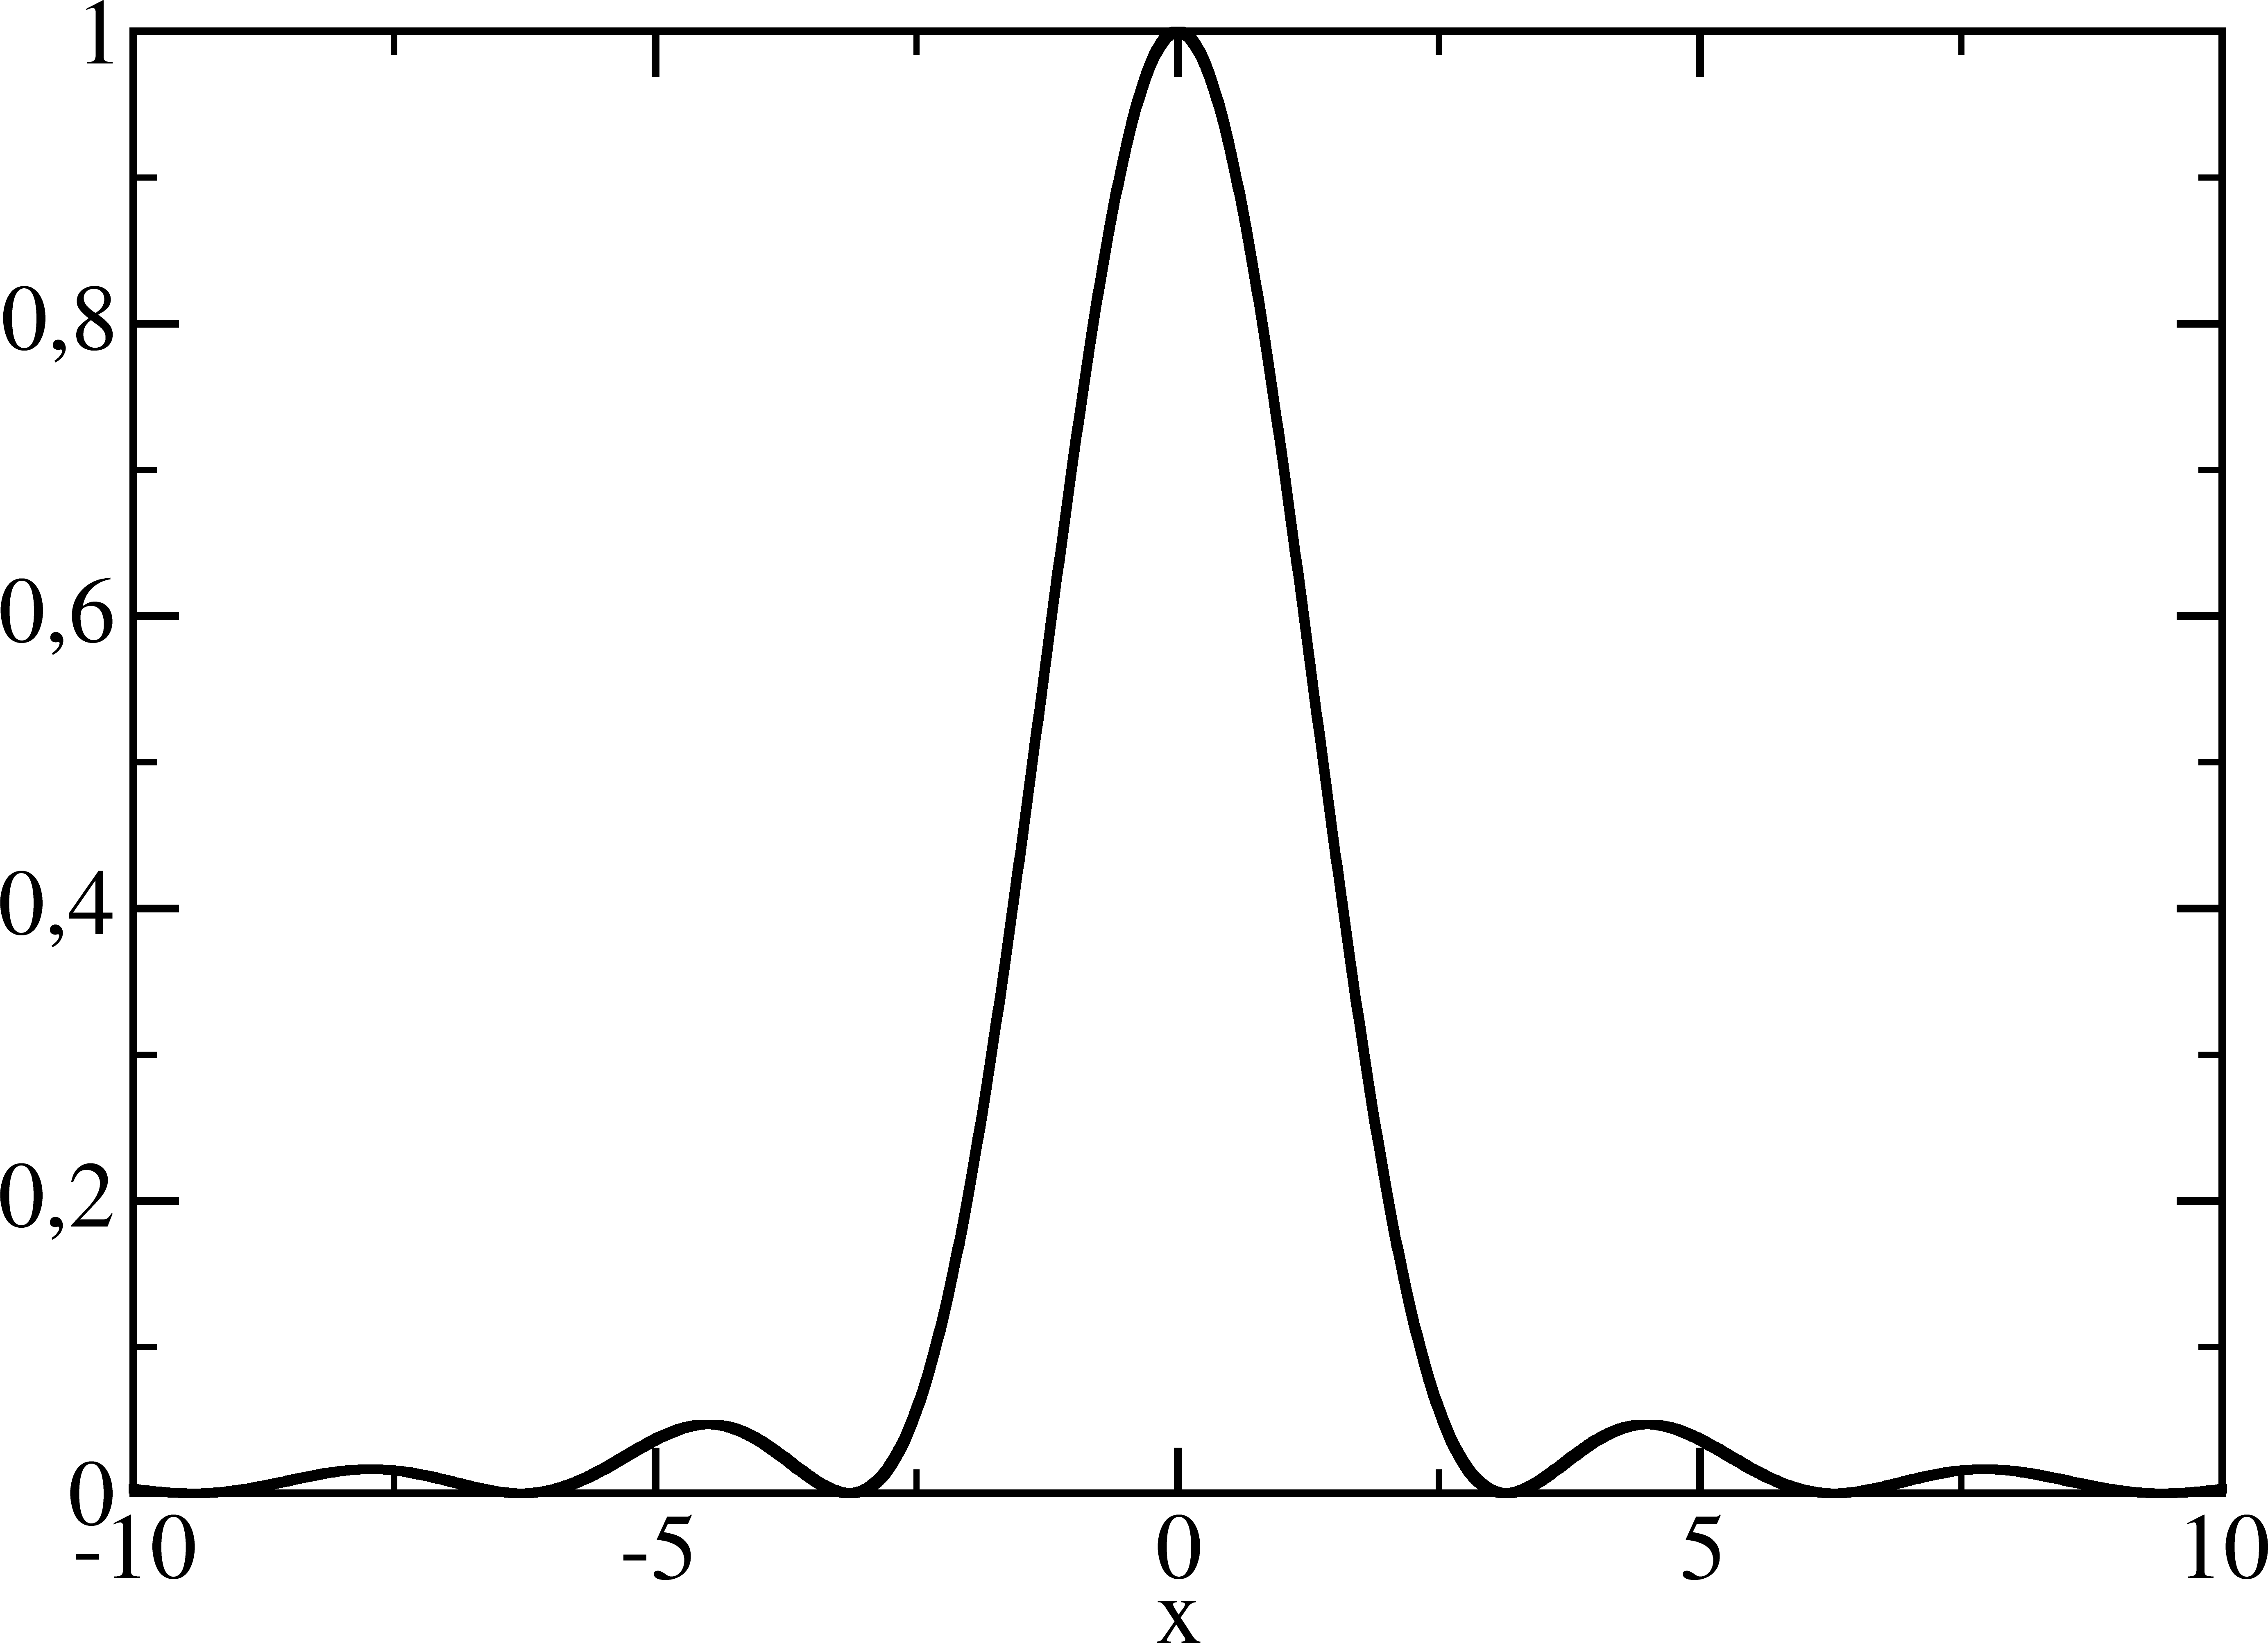
\includegraphics[width=7truecm]{slike/08_shg2.png}
\caption{Izkoristek pretvorbe v frekvenčno podvojeno valovanje je 
sorazmeren s funkcijo $(\sin(x)/x)^2$,
pri čemer je $x = \Delta k L/2$.}
\label{fig:shg2}
\end{figure}

Poglejmo primer. Faktor $\Delta k$ je različen od nič zaradi odvisnosti
lomnih količnikov od frekvence. V KH$_{2}$PO$_{4}$\index{KDP} je 
redni lomni količnik pri 1000 nm 1,496, pri 500 nm pa 1,514. Vrednost, pri kateri
pade intenziteta frekvenčno podvojenega valovanja na nič
$L_{c}=\pi /\Delta k$, je tako le okoli 30 mikrometrov. Na večjih dolžinah
postane stopnja pretvorbe zanemarljivo majhna.

Za visok izkoristek pretvorbe v frekvenčno podvojeno valovanje je torej 
pomembno, da se faze čim bolj ujemajo in da je $\Delta k = 0$. 
Takrat je vrednost faktorja $\sin(\Delta kL/2)/(\Delta kL/2)$ največja in izkoristek 
pretvorbe narašča sorazmerno s kvadratom dolžine
\beq
\frac{P_{2\omega}}{P_{\omega}}=
\frac{\omega^2 \chi_{ef}^2}{2 S n_{2\omega} n_\omega^2c_0^3\varepsilon_0} P_\omega L^2.
\eeq
Za uporabno pretvorbo v frekvenčno podvojeno valovanje je torej treba doseči 
fazno ujemanje valovnih vektorjev\index{Ujemanje faz} 
pri osnovni in podvojeni frekvenci. Kako to naredimo,
bomo spoznali v prihodnjem razdelku.

\begin{definition}
\label{deplet}
Vemo, da intenziteta frekvenčno podvojenega valovanja narašča sorazmerno s
kvadratom dolžine kristala. Takšna odvisnost velja le, če je intenziteta valovanja
pri podvojeni frekvenci bistveno manjša od intenzitete vpadnega valovanja, 
oziroma $A_3 \ll A_1, A_2$. Pokaži, da v nasprotnem primeru intenziteta frekvenčno
podvojenega valovanja $j_{2\omega}(L)$ narašča kot
\beq
j_{2\omega} (L) = j_0 \tanh^2 \left(\chi_{ef}\omega \sqrt{\frac{j_0}
{2 n_3 n_1^2 c_0^3 \varepsilon_0}} L\right),
\eeq
pri čemer je $j_0$ vpadna intenziteta valovanja pri osnovni frekvenci. Namig: upoštevaj, 
da se celotna energija ohranja.
\end{definition}

\begin{figure}[h]
\centering
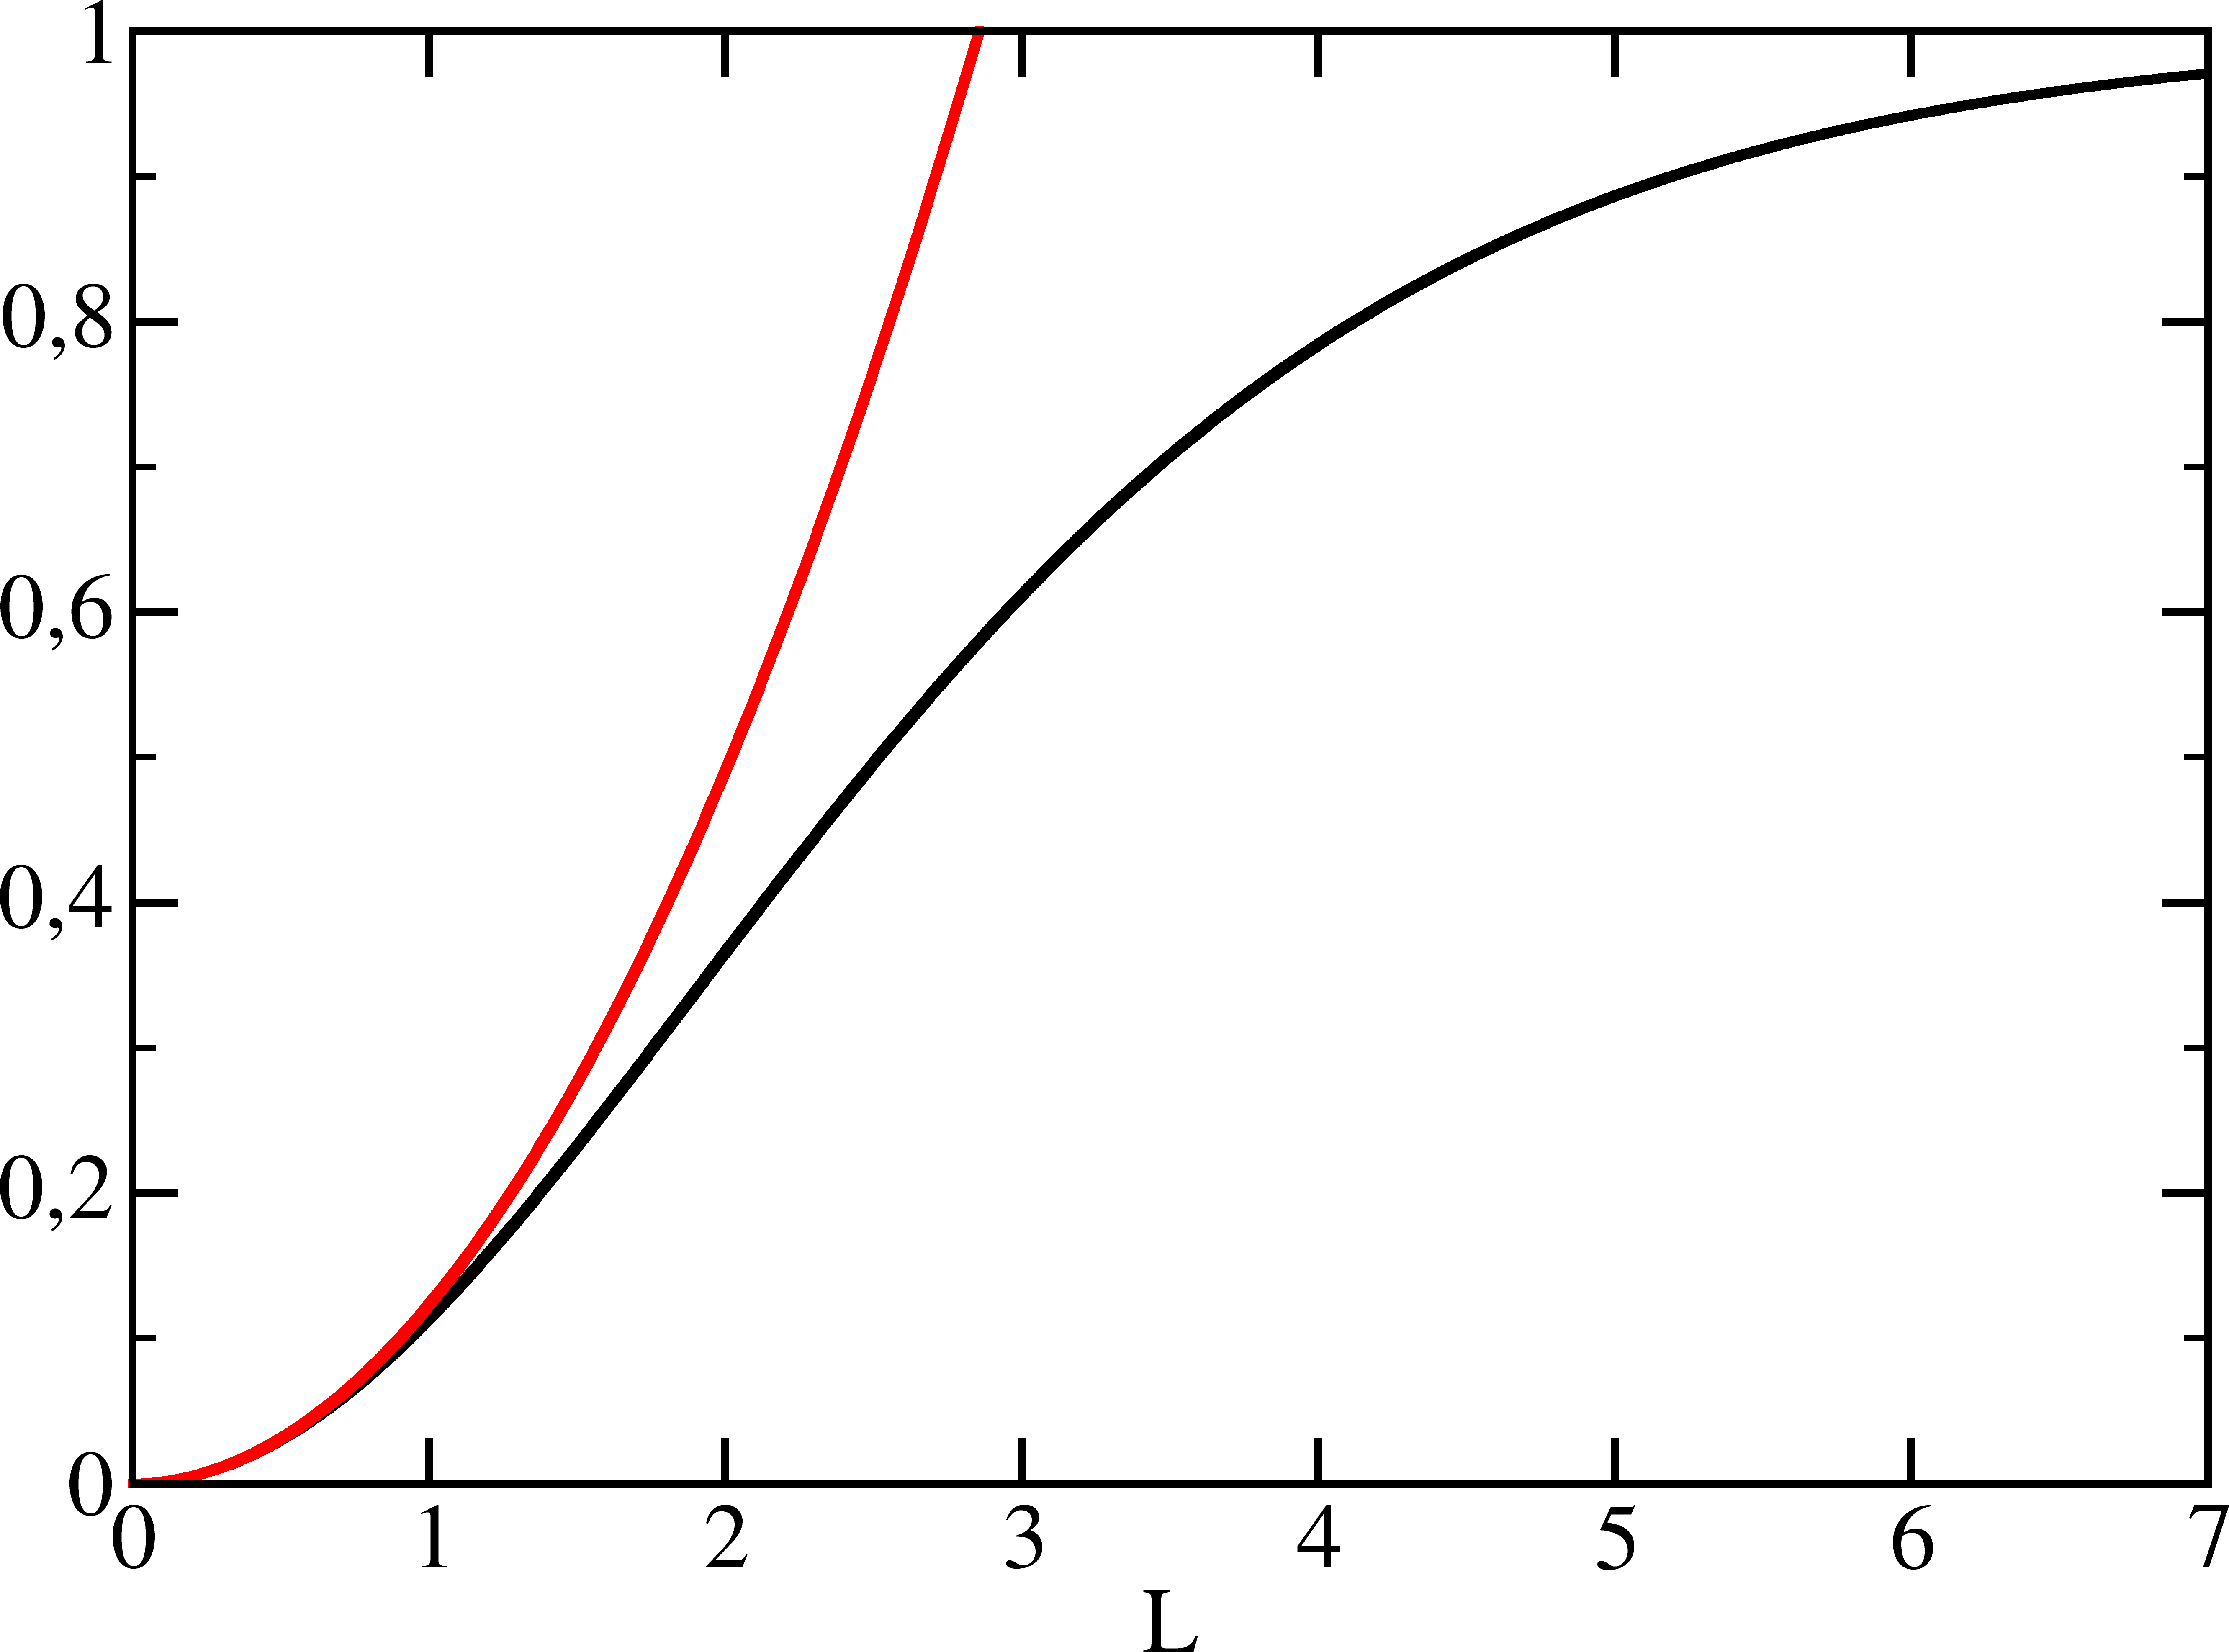
\includegraphics[width=8truecm]{slike/08_shg_depletion.png}
\caption{Izkoristek pretvorbe v frekvenčno podvojeno valovanje. Če privzamemo, da se
intenziteta osnovnega žarka ne zmanjšuje, je odvisnost parabolična (rdeča krivulja), kar 
je dober približek le za majhne intenzitete. Bolj natančen izračun pokaže, da je izkoristek 
pretvorbe sorazmeren s $\tanh^2(\kappa L)$.}
\label{fig:shg2dep}
\end{figure}

Poglejmo še, kaj se zgodi, kadar pogoj ujemanja faz ni izpolnjen in 
 $\Delta k \neq 0$. Takrat dolžino kristala $L$ v izrazu~(\ref{8.11})
pokrajšamo in izkoristek pretvorbe z naraščajočim
$L$ sinusno niha med nič in neko največjo vrednostjo. Tak pojav lahko opazimo, če
uporabimo klinast vzorec, ki se mu debelina spreminja, ali pa če vzorec sučemo 
in na ta način spreminjamo razliko faz. Ta pojav, imenujemo ga Makerjeve 
oscilacije\footnote{P. D. Maker et al., Phys. Rev. Lett. 8, 21 (1962).}, 
uporabljamo za določanje nelinearne susceptibilnost kristalov.\index{Makerjeve oscilacije}

% \begin{remark}
%  Odvisnosti stopnje pretvorbe od razlike valovnih vektorjev pri osnovni
% in podvojeni frekvenci je lahko razumeti s pomočjo slike~(\ref{fig:shg1}). Opazujmo
% prispevka k frekvenčno podvojenem valu, ki nastaneta eden na začetku kristala
% in drugi na koncu. Prispevek z začetka kristala zaradi disperzije na izhodni
% strani ni v fazi s prispevkom s konca. Pri dovolj veliki fazni razliki
% pride do destruktivne interference, ki zmanjšuje moč podvojene svetlobe.
% Razmere so podobne kot pri uklonu na široki reži, kjer prav tako seštevamo
% delna valovanja, ki se jim faza po reži linearno spreminja.
% \begin{figure}[h]
% \centering
% 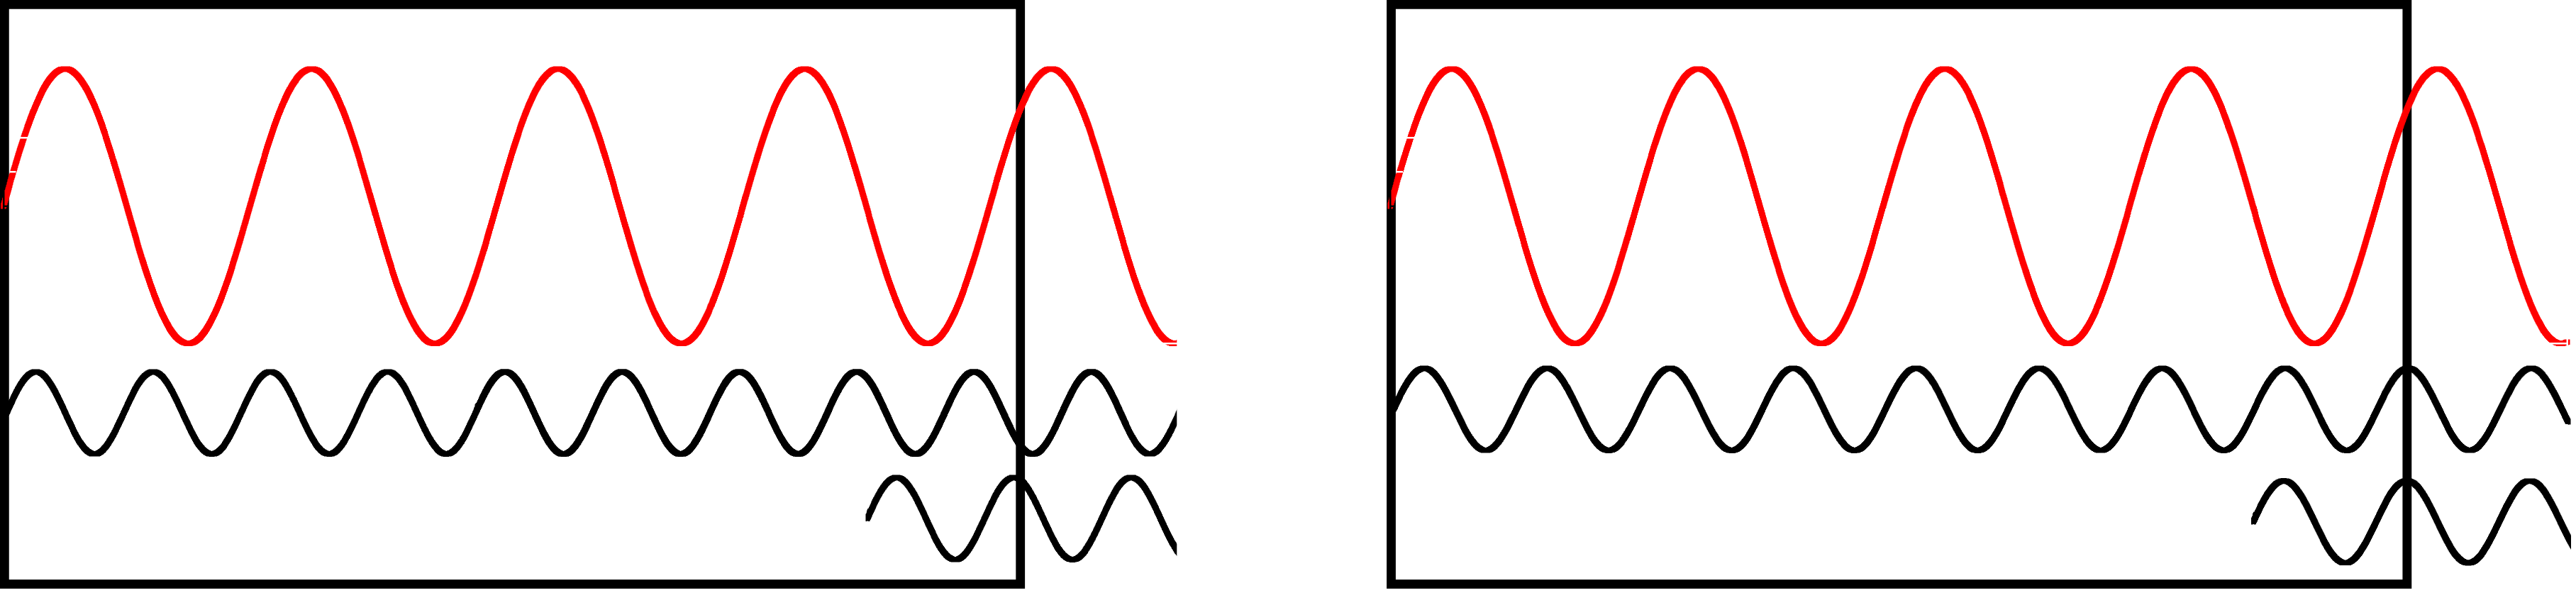
\includegraphics[width=10truecm]{slike/08_shg1.png}
% \caption{Levo: Neujemanje faz privede do destruktivne interference med valovi, ki nastajajo
% v različnih delih nelinearnega sredstva. Desno: V primeru, da se faze ujemajo, se valovanje 
% podvojeni frekvenci ojača.}
% \label{fig:shg1}
% \end{figure}
% \end{remark}

\subsection*{Ujemanje faz}
\index{Ujemanje faz}
Poglejmo, kako lahko dosežemo ujemanje faz, ki je nujno za učinkovito optično
podvajanje frekvenc. Spomnimo se, da je pogoj za ujemanje faz 
\beq
\Delta k = k_3 - k_1 -k_2 = k_3^{2\omega} - k_1^{\omega} -k_2^\omega = 
\frac{2\omega}{c_0} n_3 - \frac{\omega}{c_0} n_1- \frac{\omega}{c_0} n_2 =0.
\eeq
Iz tega sledi pogoj za ujemanje faz
\boxeq{eq:dk0}{
n_1^\omega + n_2^\omega = 2n_3^{2\omega}.
}
Da lahko zadostimo gornjemu pogoju, izkoristimo dvojni lom\index{Dvolomnost} v anizotropnih kristalih
(glej poglavje~\ref{chap:anizotropni}), pri čemer se zaradi enostavnosti omejimo le na optično 
enoosne kristale. Obravnavajmo samo kristale brez absorpcije in z normalno disperzijo, 
to pomeni, da oba lomna količnika naraščata s frekvenco.  

Za razumevanje je najbolj nazoren grafični prikaz (slika~\ref{fig:dk}). 
Podrobneje poglejmo primer s slike (a). Na njem so narisani lomni količniki
\index{Lomni količnik} za pozitivno
anizotropni ($n_e>n_o$) enoosni kristal pri enojni in dvojni
frekvenci v odvisnosti od kota glede na optično os. Rdeča barva nakazuje lomne količnike
pri vpadni frekvenci, modra pa pri podvojeni. Ekscentričnost elipse za 
izredni lomni količnik in frekvenčna disperzija sta zaradi večje nazornosti močno 
pretirani. Opazimo, da je pri nekem kotu $\vartheta$ med smerjo širjenja svetlobe $\mathbf{k}$
in optično osjo $z$ redni lomni količnik pri dvojni frekvenci enak izrednemu količniku pri osnovni
frekvenci. Če torej izberemo izredno polarizacijo vpadnega valovanja (tako, ki leži
v ravnini optične osi in smeri širjenja), bo za podvojeno valovanje z redno
polarizacijo (to je pravokotno na optično os) pri kotu
$\vartheta_m$ izpolnjen pogoj ujemanja faz~(enačba~\ref{eq:dk0}). Zapišimo to še z enačbo.

\begin{figure}[h]
\centering
\def\svgwidth{160truemm} 
\input{slike/08_phasematch.pdf_tex}
\caption{Štirje primeri, pri katerih je izpolnjen pogoj za ujemanje faz. 
(a) Ujemanje faz prvega reda za pozitivno anizotropno snov, (b)
ujemanje faz prvega reda za negativno anizotropno snov ter 
ujemanje faz drugega reda za pozitivno (c) in negativno (d) anizotropno snov.}
\label{fig:dk}
\end{figure}

Lomni količnik za redno polarizirano valovanje pri podvojeni frekvenci mora biti enak lomnemu 
količniku za izredno polarizirano valovanje pri osnovni frekvenci. Pri tem je lomni količnik
za izredno valovanje odvisen od kota
\begin{equation}
\frac{1}{(n_o^{2\omega})^2} = \frac{1}{(n^{\omega}(\vartheta))^2}=
\frac{\cos^{2}\vartheta}{(n_{o}^{\omega})^2}+\frac{\sin^{2}\vartheta}{(n_{e}^{\omega})^2}.
\label{8.12}
\end{equation}
Tako dobimo izraz
\begin{equation}
\cos^{2}\vartheta_m=\frac{(n_o^{2\omega})^{-2}-(n_{e}^{\omega})^{-2}}
{(n_{o}^{\omega})^{-2}-(n_{e}^{\omega})^{-2}},
\label{8.13}
\end{equation}
iz katerega lahko izračunamo kot $\vartheta_m$, pri katerem pride do ujemanja faz.
\begin{definition}
Pokaži, da v primeru negativne anizotropije pogoj za ujemanje faz zapišemo kot
\beq
\cos^{2}\vartheta_m=\frac{(n_o^{\omega})^{-2}-(n_{e}^{2\omega})^{-2}}
{(n_{o}^{2\omega})^{-2}-(n_{e}^{2\omega})^{-2}}.
\label{8.13a}
\eeq
\end{definition}

S slike~(\ref{fig:dk} c in d) lahko razberemo, da obstaja še en primer, pri 
katerem je izpolnjen pogoj za ujemanje faz. Poglejmo primer (c), pri katerem sta v vpadnem
valovanju prisotni obe polarizaciji, redna in izredna, podvojeno valovanje pa
je redno polarizirano. Tedaj mora biti za ujemanje faz vsota rednega in izrednega
lomnega količnika pri osnovni frekvenci enaka dvakratniku rednega lomnega 
količnika pri dvojni frekvenci. Povedano drugače: lomni količnik pri dvojni
frekvenci mora biti enak povprečju rednega in izrednega lomnega količnika
pri osnovni frekvenci. Za praktično uporabo je ta izbira, kadar obstaja,
celo ugodnejša, ker je pri njej kot ujemanja faz bliže $\pi/2$. 
Ujemanje faz je zato manj občutljivo na majhna odstopanja v kotu ali na temperaturne
spremembe lomnih količnikov. Račun kota $\vartheta_m$ za ta primer je
bolj zahteven, saj je treba rešiti enačbo četrte stopnje.

\subsection*{Efektivna susceptibilnost}
\index{Susceptibilnost!nelinearna, efektivna}
Na izhodno moč frekvenčno podvojenega snopa poleg faznega faktorja bistveno vpliva tudi efektivna 
susceptibilnost $\chi_{ef}$, ki jo moramo izračunati za vsak primer posebej. 
V optično enoosnem kristalu
je kriterij ujemanja faz izpolnjen na stožcu okoli optične osi, pri čemer je stožec določen 
z izračunanim kotom $\vartheta_m$ (enačbi~\ref{8.13} in \ref{8.13a}). 
Drugi kot, ki določa smer širjenja v ravnini, ki je pravokotna na optično os, pa 
izberemo tako, da izkoristimo največje komponente nelinearne 
susceptibilnosti. 

Oglejmo si kot primer spet KH$_{2}$PO$_{4}$\index{KDP}, ki je negativno anizotropen 
z vrednostmi $n_o^{\omega} = 1,4942$, 
$n_e^{\omega} = 1,4603$, $n_o^{2\omega} = 1,5129$ in $n_e^{2\omega} = 1,4709$
(slika~\ref{fig:dk}\,b). Valovna dolžina osnovnega snopa naj bo 1064~nm. 
Po podatkih, navedenih zgoraj, izračunamo po enačbi~(\ref{8.13a}) za kot ujemanja faz 
$\vartheta_m = 41,25^\circ$. Nelinearna susceptibilnost ima v tetragonalni
simetriji $\bar{4}2m$ od nič različne komponente $\chi_\textrm{xyz}$, $\chi_\textrm{xzy}$
$\chi_\textrm{zxy}$, $\chi_\textrm{zyx}$, $\chi_\textrm{yzx}$ in $\chi_\textrm{yxz}$
(glej tabelo~\ref{table:chi}). 
Zaradi poenostavitve privzamemo, da so njihove vrednosti enake. 

Naj se osnovno in frekvenčno podvojeno valovanje širita 
v smeri $\mathbf{s}$. Pri zapisu vektorja si pomagamo 
s sliko (\ref{fig:chi})
\begin{equation}
\mathbf{s}=(\cos\varphi\sin\vartheta_m,\sin\varphi\sin\vartheta_m,\cos\vartheta_m),
\label{8.14}
\end{equation}
kjer je $\varphi$ kot med osjo $x$ in projekcijo $\mathbf{s}$ na ravnino
$xy$. Naša naloga je poiskati vrednost kota $\varphi$, pri kateri je 
moč frekvenčno podvojenega valovanja največja.
\begin{figure}[h]
\centering
\def\svgwidth{70truemm} 
\input{slike/08_chi.pdf_tex}
\caption{K izračunu efektivne susceptibilnosti. Rdeč vektor označuje
polarizacijo vhodnega valovanja, moder pa polarizacijo frekvenčno podvojenega valovanja.}
\label{fig:chi}
\end{figure}
Iz pogoja za ujemanje faz vidimo, da mora biti vpadna svetloba redno polarizirana, 
izhodna frekvenčno podvojena pa izredno polarizirana. Redna polarizacija je pravokotna na 
os $z$ (optično os) in hkrati pravokotna na smer vektorja $\mathbf{s}$. Zapišemo jo kot
\begin{equation}
\mathbf{e}_o=(\sin\varphi,-\cos\varphi,0).
\label{8.15}
\end{equation}
Izredna polarizacija leži v ravnini, ki jo tvori vektor $\mathbf{s}$ z osjo $z$,
hkrati pa je pravokotna na vektor $\mathbf{s}$, 
tako da jo zapišemo kot 
\begin{equation}
\mathbf{e}_e=(-\cos \varphi \cos \vartheta_m,-\sin \varphi \cos \vartheta_m ,\sin \vartheta_m).
\label{8.15a}
\end{equation}
Spomnimo se, da efektivno susceptibilnost izračunamo kot (enačba~\ref{eq:chicomp})
\beq
\chi_{ef} = \sum_{ijk} \chi_{ijk} e_{3i} e_{1j} e_{2k} = \sum_{ijk} \chi_{ijk} e_{ei} e_{oj} e_{ok}.
\eeq
Krajši račun pokaže, da je zaradi oblike tenzorja nelinearne susceptibilnosti v izbranem 
primeru od nič različna le $z$ komponenta nelinearne polarizacije. Zapišemo
\beq
\chi_{ef} = \chi_{\textrm{zxy}} e_{ez} e_{ox} e_{oy} + \chi_{\textrm{zyx}} e_{ez} e_{oy} e_{ox}
\eeq
in
\begin{eqnarray}
P_{\textrm{z}}^{2\omega}&=&- 2\varepsilon_0\, \chi_{\textrm{zxy}}E_{0}^2\cos\varphi\sin\varphi
\sin\vartheta_m \nonumber \\
&=& - \varepsilon_0\, \chi_{\textrm{zxy}}E_{0}^2\sin(2\varphi) \sin\vartheta_m.
\label{8.151}
\end{eqnarray}
Nelinearna polarizacija je največja, kadar je $\varphi=\pi/4$.
Največji efektivni koeficient $\chi_{ef}$, ki nastopa v izrazih za amplitudo in 
moč podvojene svetlobe (enačbi~\ref{8.10} in \ref{8.11}), je torej v izbranem primeru 
\begin{equation}
\chi_{ef}= 
\sin\vartheta_m \chi_{\textrm{zxy}} \approx 0,66\, \chi_{\textrm{zxy}} \approx 0,74~\mathrm{pm/V}.
\label{8.16}
\end{equation}

\begin{definition}
Izračunaj efektivno nelinearno susceptibilnost za frekvenčno podvajanje svetlobe z valovno
dolžino 10~$\mu$m v kristalu telurja s simetrijsko grupo 32 (glej tabelo~\ref{table:chi}). 
Lomni količniki: $n_o^{\omega} = 4,7969$, 
$n_e^{\omega} = 6,2455$, $n_o^{2\omega} = 4,8657$ in $n_e^{2\omega} = 6,3152$.
\end{definition}

\section{Frekvenčno podvajanje Gaussovih snopov}
\index{Optično podvajanje frekvenc}
Doslej smo vpadni in frekvenčno podvojeni snop obravnavali kot ravni valovanji,
ki sta bili razsežni v prečni smeri. Izračunali smo, da v primeru \index{Ujemanje faz}
ujemanja faz ($\Delta k=0$)
moč frekvenčno podvojene svetlobe narašča s kvadratom dolžine poti po nelinearnem
sredstvu. Pretvorba v frekvenčno podvojeno svetlobo je po enačbi~(\ref{8.11}) tem
učinkovitejša, čim večja je gostota svetlobnega toka pri osnovni frekvenci.
Zato v praksi vpadno svetlobo vselej fokusiramo in tako povečamo gostoto toka.  

Poglejmo, kako se enačbe spremenijo, če je vpadni snop pri osnovni 
frekvenci Gaussove oblike\index{Gaussov snop!frekvenčno podvajanje}. 
Rezultat lahko ocenimo, če vzamemo, da je
efektivna dolžina za pretvorbo $L$ kar dolžina grla; izven grla je 
gostota toka znatno manjša kot v grlu, s tem pa tudi izkoristek pretvorbe v 
frekvenčno podvojeni snop.
Dolžina grla je 
\beq
L=2z_{0}=\frac{2n \pi w_{0}^{2}}{\lambda} = \frac{n w_0^2 \omega}{c_0}.
\label{SHGG}
\eeq
Tako je presek vpadnega snopa
\beq
S=\pi w_{0}^{2} = \frac{\pi c_0 L}{n \omega.}
\eeq
Daljše ko je grlo in večja dolžina $L$, na kateri pride do frekvenčnega podvajanja, 
večji je tudi presek snopa $S$ in zato manjša intenziteta svetlobe, kar zmanjša
učinek pretvorbe v frekvenčno podvojeno valovanje.
Vstavimo $S$ v enačbo~(\ref{8.11}), upoštevamo ujemanje faz in dobimo 
\boxeq{8.17}{
\frac{P_{2\omega}}{P_{\omega}}=
\frac{\omega^3 \chi_{ef}^2}{2 \pi n_{2\omega} n_\omega c_0^4\varepsilon_0} P_\omega\, L.
}
Ob optimalnem fokusiranju je torej izkoristek pretvorbe sorazmeren z 
dolžino kristala in ne z njenim kvadratom.

\begin{definition}
Imamo 1~cm dolg kristal KH$_{2}$PO$_{4}$. Valovna dolžina vpadne svetlobe 
je 1,06~$\mu$m, vhodna moč $P_\omega = 10$~kW, efektivna nelinearna susceptibilnost
$\chi_{ef}=7\cdot10^{-13}~$m/V, $\Delta k=0$ in $n=1,5$. Pokaži, da je
faktor pretvorbe v frekvenčno podvojeno svetlobo okoli $20~\%$.

Da je dolžina grla $2z_{0}=1$~cm, mora biti polmer
grla okoli 40~$\mu$m. Gostota svetlobnega toka v kristalu je pri
tem $2\cdot10^{8}$~W/cm$^{2}$, kar je že blizu praga za poškodbe,
predvsem na vstopni ali izstopni površini. Zato je pri podvajanju frekvenc
zelo pomembna odpornost nelinearnega kristala proti poškodbam
zaradi velike gostote svetlobnega toka. To in možnost izpolnitve kriterija ujemanja 
faz sta poglavitna kriterija pri izbiri snovi za frekvenčno podvajanje. 
\end{definition}

\section{{*}Račun podvajanja Gaussovih snopov}
\index{Gaussov snop!frekvenčno podvajanje}
V prejšnjem razdelku smo na hitro grobo ocenili vpliv oblike Gaussovih snopov
na frekvenčno podvajanje. Naredimo zdaj še natančnejši izračun. Vrnimo se k valovni
enačbi~(\ref{8.3}), vpadna snopa naj bosta pri frekvencah
$\omega_{1}$ in $\omega_{2}$, nastajajoč snop pa pri frekvenci
$\omega_{3}=\omega_{1}+\omega_{2}$.
Podobno kot prej naj ima vsako od polj obliko 
\beq
\mathbf{E}_{i}  = \frac{\mathbf{e}_{i}}{2}\left[\tilde{A}_{i}(r,z)\, 
e^{i(k_{i}z-\omega_{i}t)}+\tilde{A}_{i}^{*}(r,z)\, e^{-i(k_{i}z-\omega_{i}t)}\right],
\eeq
pri čemer je $\tilde{A}(r,z)$ zdaj funkcija tako vzdolžne kot tudi prečne koordinate. Privzeli
bomo, da se vzdolž $z$ le počasi spreminja.
Zaradi poenostavljenega zapisa vpeljimo novo spremenljivko 
\beq
\psi_i = \sqrt{\frac{n_i}{\omega_i}}\tilde{A}_i.
\eeq
Tako je nastavek za električno poljsko jakost
\begin{equation}
\mathbf{E}_{i}=\frac{\mathbf{e}_{i}}{2}\sqrt{\frac{\omega_{i}}{n_{i}}}\psi_{i}(r,z)
e^{i(k_{i}z-\omega_{i}t)}+\mbox{ k. k.}
\label{8.18}
\end{equation}
Vstavimo nastavek~(\ref{8.18}) v valovno
enačbo~(\ref{8.3}) in ločimo na levi in desni člene z enako frekvenco.
Zaradi počasnega spreminjanja vzdolž smeri $z$ lahko zanemarimo tudi druge odvode 
$\psi$ po $z$. Od tod sledi sklopljen sistem obosnih enačb 
\begin{eqnarray}
\nabla_{\perp}^{2}\psi_{1}+2ik_{1}\psi_{1}^{\prime} & = & -
\frac{k_{1}}{2}\kappa\psi_{2}^{\ast}\psi_{3}e^{-i\Delta kz}\\
\nabla_{\perp}^{2}\psi_{2}+2ik_{2}\psi_{2}^{\prime} & = & -
\frac{k_{2}}{2}\kappa\psi_{1}^{\ast}\psi_{3}e^{-i\Delta kz}\\
\nabla_{\perp}^{2}\psi_{3}+2ik_{3}\psi_{3}^{\prime} & =
& - \frac{k_{3}}{2}\kappa\psi_{1}\psi_{2}e^{i\Delta kz}
\label{SHGGauss_3}
\end{eqnarray}
s pripadajočim sistemom konjugiranih enačb. Pri tem je 
\begin{equation}
\kappa=\frac{\chi_{ef}}{c_0} \sqrt{\frac{\omega_{1}\omega_{2}\omega_{3}}{n_{1}n_{2}n_{3}}}.
\label{8.20}
\end{equation}
S črtico smo označili odvajanje po $z$. Gornji sistem enačb je očitno
posplošitev sistema enačb~(\ref{eq:nlAz} do \ref{eq:nlA3}) za primer, ko je valovanje odvisno
tudi od prečne koordinate. Reševanje tega nelinearnega sistema parcialnih
diferencialnih enačb je v splošnem zelo zapleteno.

Poglejmo le najenostavnejši primer frekvenčnega podvajanja, ko je 
$\omega_{3}=2\omega_{1}=2\omega$.
Vpadna snopa naj bosta enaka in Gaussove oblike~(enačba~\ref{eq:gaussov-snop}), 
njuna amplituda pa naj bo enaka $A_1$
\begin{equation}
\psi_{1} = \psi_2 = A_{1}\frac{1}{1+iz/z_1}
\exp\left(-\frac{r^{2}}{w_1^{2}(z)}+\frac{ik_1r^{2}}{2R_1(z)}\right).
\label{8.21}
\end{equation}
Privzemimo še, da je izpolnjen pogoj za ujemanje faz\index{Ujemanje faz}, $\Delta k=0$,
in da je $\psi_{3}$ dovolj majhen, da nam zmanjševanja $\psi_{1}$
ni treba upoštevati. Tudi za podvojeni snop privzemimo Gaussovo 
obliko, njegova amplituda $A_3$ pa naj le počasi narašča. Zapišemo ga kot
\begin{equation}
\psi_{3}=A_{3}(z)\psi_{3H}(z,r)=A_{3}(z)\frac{1}{1+iz/z_{3}}
\exp\left(-\frac{r^{2}}{w_{3}^{2}(z)}+\frac{ik_{3}r^{2}}{2R_{3}(z)}\right),
\label{8.22}
\end{equation}
pri čemer $\psi_{3H}$ reši homogeno obosno valovno 
enačbo~(\ref{eq:obosna-valovna-enacba})\index{Obosna valovna enačba}. Ko izraza za $\psi_{1}$
in $\psi_{3}$ vstavimo v tretjo enačbo sistema sklopljenih enačb (\ref{SHGGauss_3}),
ostane na levi le člen oblike $2ik_{3}A_{3}^{\prime}(z)\psi_{3H}$. Tako dobimo pogoj
\begin{equation}
A_{3}^{\prime}(z)\frac{1}{1+iz/z_3}\exp\left(-\frac{r^{2}}{w_{3}^{2}(z)}+\frac{ik_{3}r^{2}}
{2R_{3}(z)}\right)=
\frac{i\kappa}{4}A_{1}^{2}\frac{1}{(1+iz/z_{1})^{2}}\exp\left(-\frac{2r^{2}}
{w_{1}^{2}(z)}+\frac{ik_{1}r^{2}}{R_{1}(z)}\right).
\label{8.23}
\end{equation}
Poiščimo rešitev te enačbe v obliki, za katero velja $w_{30}^{2}=w_{10}^{2}/2$. Tedaj je 
\beq
z_{3}=\frac{k_{3}w_{30}^{2}}{2}=\frac{2k_{1}w_{10}^{2}}{4}=z_{1}
\eeq
in je tudi $w_{3}^{2}(z)=w_{1}^{2}(z)/2$. Poleg tega je $R_{3}(z)=R_{1}(z)$
in lahko na obeh straneh pokrajšamo eksponentna faktorja. Ostane 
\begin{equation}
A_{3}^{\prime}(z)=\frac{i\kappa}{4}A_{1}^{2}\frac{1}{1+iz/z_1}.
\label{8.24}
\end{equation}
Gornjo enačbo seveda brez težav integriramo. Naj bo grlo vpadnega
snopa ravno na sredini nelinearnega sredstva, tako da integriramo
od $-L/2$ do $L/2$
\begin{eqnarray}
A_{3}(L) & = & \frac{i\kappa}{4}A_{1}^{2}\int_{-L/2}^{L/2}\frac{dz}{1+iz/z_1} 
  = \frac{\kappa}{4}A_{1}^{2}z_{1}\ln\frac{1+i\frac{L}{2z_{1}}}{1-i\frac{L}{2z_{1}}}= \nonumber \\
 & = & \frac{\kappa}{2}A_{1}^{2}z_{1}\arctan\frac{L}{2z_{1}}\;.
\end{eqnarray}
Moč Gaussovega snopa je
\begin{equation}
P_{i}=\pi w_{i0}^{2} \frac{1}{2}c_0 n_i \epsilon_{0}E_{i0}^{2}=
\frac{\pi}{2}w_{i0}^{2}\varepsilon_0 c_0 \omega_{i} A_{i}^{2},
\label{8.26}
\end{equation}
tako da je izkoristek pri frekvenčnem podvajanju Gaussovega snopa 
\begin{equation}
\frac{P_{2\omega}}{P_{\omega}}=\frac{A_3^2}{A_1^2} = 
\frac{\chi_{ef}^2 \omega^3 P_\omega z_1}{2 \pi c_0^4 \varepsilon_0 n_1 n_3} 
\arctan^2 \left( \frac{L}{2z_1}\right)
= \frac{\chi_{ef}^2 \omega^3 P_\omega}{2 \pi c_0^4 \varepsilon_0 n_1 n_3} \frac{L}{2}
\arctan^2 \left( \frac{L}{2z_1}\right) \frac{1}{L/2z_1}.
\label{8.27}
\end{equation}
Funkcija $(\arctan^{2}x)/x$ zavzame največjo vrednost 0,64 pri $x =L/2z_1=1,39$.
Pri dani dolžini nelinearnega sredstva $L$ je torej 
izkoristek največji, kadar je $z_{1}=0,36\,L$, kar je malo manj kot pri
preprosti oceni $z_{1}=0,5\,L$ (enačba~\ref{SHGG}). Največji izkoristek
frekvenčnega podvajanja Gaussovih snopov je tako
\begin{equation}
\frac{P_{2\omega}}{P_{\omega}}
= 0,32 \frac{\chi_{ef}^2 \omega^3 }{2 \pi c_0^4 \varepsilon_0 n_1 n_3} P_\omega L.
\label{8.28}
\end{equation}
To je malo manj od preproste ocene, ki smo jo naredili v prejšnjem razdelku (enačba~\ref{8.17}),
v obeh primerih pa izkoristek narašča linearno z dolžino kristala.

\section{Optično parametrično ojačevanje}
\index{Optično parametrično ojačevanje}
\index{Parametrično ojačevanje|see{Optično parametrično ojačevanje}}

Oglejmo si še en zelo uporaben primer mešanja treh valovanj, 
ki ga opisujejo enačbe (\ref{eq:nlAz}) do (\ref{eq:nlA3}). Gre za
optično parametrično ojačevanje, pri katerem nelinearne optične pojave
izkoristimo za ojačevanje optičnih signalov. Imejmo vhodni
signal pri frekvenci $\omega_{1}$, ki ga želimo ojačati, in močno črpalno valovanje
pri frekvenci $\omega_{3}>\omega_{1}$. Zaradi nelinearnosti v snovi se 
intenziteta valovanja pri $\omega_{1}$ povečuje, 
intenziteta valovanja pri $\omega_{3}$ zmanjšuje, hkrati pa zaradi
ohranitve energije nastaja dodatno valovanje pri razliki frekvenc
$\omega_{2}=\omega_{3}-\omega_{1}$. Proces parametričnega ojačevanja 
si torej lahko predstavljamo kot pretvorbo enega fotona pri frekvenci 
$\omega_{3}$ v dva fotona pri $\omega_{1}$ in $\omega_{2}$.
Parametrično ojačevanje pogosto uporabljamo za ojačevanje šibkih signalov 
v infrardečem območju.
\begin{figure}[h]
\centering
\def\svgwidth{100truemm} 
\input{slike/08_opa.pdf_tex}
\caption{Shematski prikaz nastanka valovanj pri optičnem parametričnem ojačevanju}
\label{fig:opa2}
\end{figure}

Izhajamo iz splošnih enačb za nelinearne optične pojave drugega reda (enačbe~\ref{eq:nlAz} do
\ref{eq:nlA3}). 
\begin{eqnarray}
\frac{dA_{3}}{dz} &=& \frac{i\omega_{3}\chi_{ef}}{4c_0 n_3} A_{1}\, A_{2}\, e^{-i\Delta kz}\\
\frac{dA_{2}}{dz} &=&\frac{i\omega_{2}\chi_{ef}}{4c_0 n_2} A_{1}^*\, A_{3}\, e^{i\Delta kz}\\
\frac{dA_{1}}{dz} &=&\frac{i\omega_{1}\chi_{ef}}{4c_0 n_1} A_{2}^*\, A_{3}\, e^{i\Delta kz}.
\label{eq:opaA}
\end{eqnarray}
Privzemimo, da je črpalno valovanje vselej dosti močnejše od drugih dveh
($A_{3}\gg A_{1}$, $A_{2}$) in njegova jakost približno konstantna $A_3 = A_{30}$.
Poskrbimo še, da je izpolnjen pogoj za ujemanje faz, $\Delta k=0$, 
začetna pogoja pa zapišemo kot $A_{1}(z=0)=A_{10}$ in $A_{2}(z=0)=0$. Ko vse to upoštevamo,
dobimo dve sklopljeni enačbi
\begin{eqnarray}
\frac{dA_{1}}{dz} &=& \frac{i\omega_{1}\chi_{ef}}{4c_0 n_1} A_{2}^*\, A_{30}\label{eq:opaA1} 
\qquad \mathrm{in} \\
\frac{dA_{2}^*}{dz} &=& -\frac{i\omega_{2}\chi_{ef}}{4c_0 n_2} A_{1}\, A_{30}^*.
\label{eq:opaA2}
\end{eqnarray}
Enačbi lahko rešimo, tako da prvo odvajamo po $z$ in vanjo vstavimo drugo enačbo.
Sledi
\beq
\frac{d^2 A_1}{d z^2} = \frac{\omega_1 \omega_2 \chi_{ef}^2|A_{30}|^2}
{16 c_0^2 n_1 n_2} A_1 = \kappa^2 A_1
\eeq
in podobno za $A_2$
\beq
\frac{d^2 A_2}{d z^2} = \frac{\omega_1 \omega_2 \chi_{ef}^2|A_{30}|^2}
{16 c_0^2 n_1 n_2} A_2 = \kappa^2 A_2.
\eeq
Ob upoštevanju začetnih pogojev izračunamo rešitev za naraščanje amplitude signalnega žarka
z začetno amplitudo $A_{10}$
\boxeq{eq:opa}{
A_1 = A_{10} \cosh (\kappa L).
}
Hkrati z njim narašča tudi amplituda dodatnega nedejavnega ({\it idle}) žarka, ki nastane
med procesom ojačanja
\boxeq{eq:opan}{
A_2 = A_{20} \sinh (\kappa L).
}
V gornjih enačbah je $L$ dolžina nelinearnega sredstva, 
\beq
\kappa^2 = \frac{\omega_1 \omega_2 \chi_{ef}^2|A_{30}|^2}
{16 c_0^2 n_1 n_2} 
\label{opakapa}
\eeq
in
\beq
A_{20} = i \sqrt{\frac{\omega_2 n_1}{\omega_1 n_2}} A_{10}.
\label{opakapaA}
\eeq
Na začetku intenziteti obeh valovanj naraščata približno eksponentno na račun črpalnega
valovanja. Ko postane njuna intenziteta znatna in se začne $A_3$ zmanjševati, je treba to seveda
tudi upoštevati pri izračunu. V tem primeru je treba rešiti bolj zahteven sistem treh 
sklopljenih enačb, podobno~\textendash~a še bolj zapleteno~\textendash~kot v nalogi~(\ref{deplet}).

\begin{definition}
Pokaži, da sta izraza za amplitudi polji $A_1$ in $A_2$ (enačbi~\ref{eq:opa} in~\ref{eq:opan})
rešitvi sklopljenih enačb~(\ref{eq:opaA1}) in (\ref{eq:opaA2}) ob parametrih $A_{20}$ in $\kappa$, kot sta zapisana v enačbah~(\ref{opakapa}) in (\ref{opakapaA}).
\end{definition}

Do zdaj smo vedno privzeli, da je izpolnjen pogoj ujemanja faz \index{Ujemanje faz}
in $\Delta k=k_{3}-k_{1}-k_{2}=0$. 
Ta pogoj lahko izpolnimo na enak način kot pri podvajanju frekvence: v dvolomnem kristalu 
izberemo ustrezno smer glede na optično os in ustrezne polarizacije, 
tako da velja $\omega_{3}n_{3}=\omega_{1}n_{1}+\omega_{2}n_{2}$.

Lahko na primer vzamemo izredno polarizacijo za črpalno valovanje
in redni polarizaciji za obe ojačevani valovanji, podobno kot pri
podvajanju frekvence. Tedaj mora biti izpolnjen naslednji pogoj 
\begin{equation}
\left[\left(\frac{\cos\vartheta_{m}}{n_{o}^{\omega_{3}}}\right)^{2}
+\left(\frac{\sin\vartheta_{m}}{n_{e}^{\omega_{3}}}\right)^{2}\right]^{-1/2}=
\frac{\omega_{1}}{\omega_{3}}n_{o}^{\omega_{1}}+\frac{\omega_{2}}{\omega_{3}}n_{o}^{\omega_{2}}.
\label{8.34}
\end{equation}

\begin{figure}[h]
\centering
\def\svgwidth{90truemm} 
\input{slike/08_opagraf.pdf_tex}
\caption{Normirani intenziteti ojačanega žarka in dodatnega žarka, ki nastane zaradi ohranitve
energije. Naraščajoči funkciji sta seveda samo približek, ki velja, dokler je ojačanje majhno in 
se intenziteta črpalnega žarka ne zmanjšuje znantno.}
\label{fig:opagraf}
\end{figure}

\begin{definition}
Obravnavali smo optično parametrično ojačevanje, ko je bil izpolnjen kriterij za ujemanje faz. 
Pokaži, v primeru neujemanja faz $\Delta k \neq 0$ amplitudi ojačevanega in dodatnega 
žarka naraščata kot \index{Neujemanje faz}
\beq
A_1 = A_{10} \left( \cosh(\kappa z) - \frac{i \Delta kz}{2 \kappa} \sinh (\kappa z) 
\right) e^{\frac{i \Delta kz}{2}}\\
A_2 = A_{20} \sinh(\kappa z) e^{\frac{i \Delta k}{2}},
\eeq
pri čemer sta
\beq
\kappa^2 = \frac{\omega_1 \omega_2 \chi_{ef}^2|A_{30}|^2}
{16 c_0^2 n_1 n_2} - \frac{\Delta k^2}{4} \quad \mathrm{in} \quad
A_{20} = i \sqrt{\frac{\omega_2 n_1}{\omega_1 n_2}} \sqrt{1 + \frac{\Delta k^2}{4 \kappa^2}}
~A_{10}.
\eeq
Hitro uvidimo, da so gornje enačbe v limitnem primeru $\Delta k = 0$ enake 
enačbam~(\ref{eq:opa}, \ref{eq:opan} in \ref{opakapa}).
\end{definition}

Za konec ocenimo koeficient ojačanja v nelinearnem kristalu 
LiNbO$_{3}$\index{LiNbO$_3$}, v katerem želimo
ojačati svetlobo z valovno dolžino $\lambda = 1~\mu$m. Črpajmo z laserjem z valovno dolžino 
okoli 500~nm in gostoto svetlobnega toka 5~MW/cm$^{2}$. Lomni količnik snovi je 
$n = 2,2$, $\chi_{ef} = 5$~pm/V. Vstavimo podatke v enačbo~(\ref{opakapa}) in dobimo vrednost
$\kappa \sim 0,15$/cm. Faktor ojačanja vpadne intenzitete svetlobe v 1~cm dolgem kristalu je 
tako le približno $2~\%$. 

\subsection*{Optični parametrični oscilator (OPO)}
\index{Optični parametrični oscilator}
Gornji izračun kaže, da optično parametrično ojačevanje pri prehodu skozi kristal ni prav veliko
kljub dokaj močnemu črpalnemu žarku. Zato je smiselno, da svetloba skozi ojačevalno 
sredstvo preide večkrat in se postopoma ojačuje. To naredimo tako, 
da optično ojačevalno sredstvo zapremo v optični 
resonator\index{Resonator!parametrični oscilator}
in signal se ob vsakem obhodu ojača. Sestavili smo t.\,i.\,optični parametrični oscilator. 
\begin{figure}[h]
\centering
\def\svgwidth{100truemm} 
\input{slike/08_opo.pdf_tex}
\caption{Shematski prikaz tipičnega optičnega parametričnega oscilatorja. Ojačevalno sredstvo
zapremo med resonatorja, da se signalni žarek ($\omega_1$) ob vsakem preletu ojači.}
\label{fig:opo}
\end{figure}

V optičnemu resonatorju je odbojnost zrcal za črpalni žarek ($\omega_3$) zelo majhna, 
odbojnost za ojačani žarek pa blizu ena. Valovanje pri $\omega_1$,
ki se v parametričnem oscilatorju ojačuje, nastane spontano, prav tako valovanje pri 
$\omega_2 = \omega_3 -\omega_1$. Njuni frekvenci sta dodatno določeni s pogojem za 
ujemanje faz $ k_3 - k_1 - k_2 = 0$, 
hkrati pa mora ojačevano nihanje sovpadati z lastnim nihanjem resonatorja. 
S sukanjem ojačevalnega kristala lahko na ta način spreminjamo
ojačano frekvenco in naredili smo nastavljiv izvor svetlobe, navadno infrardeče. 

Za delovanje oscilatorja biti jakost črpalnega žarka tako velika, da je parametrično 
ojačevanje na obhod večje od izgub. Izračunajmo za primer prag simetričnega oscilatorja. Signal z močjo 
$P_0$ se ob prehodu skozi ojačevalno sredstvo ojača (enačba~\ref{eq:opa})
\beq
P_1 = P_0 \cosh^2 (\kappa L),
\eeq
hkrati pa se zaradi delno prepustnih zrcal z odbojnostjo $R$ intenziteta žarka zmanjšuje. 
Pri tem ne pozabimo, da je pogoj ujemanja faz izpolnjen le v eni smeri in se svetloba
ojačuje le enkrat na celoten obhod. Ob preletu v drugo smer je namreč $\Delta k \neq 0$ in žarek se ne ojačuje.
Moč žarka po obhodu $P_2$ je enaka začetni moči $P_0$, saj je pri pragu ojačanje ravno enako izgubam 
\beq
P_2 = R^2 P_1 = R^2 P_0 \cosh^2 (\kappa L) = P_0
\eeq
oziroma
\beq
R^2 \cosh^2 (\kappa L) =1.
\eeq
Iz gornjega pogoja določimo parameter $\kappa$, po enačbi~(\ref{opakapa}) pa mejno 
amplitudo in intenziteto črpalnega žarka. Nadaljujmo še prejšnji primer ojačanja 
svetlobe v 1~cm dolgem kristalu LiNbO$_{3}$.
Če je odbojnost zrcal $R=0,9$ in prečni presek žarka $10~\mu$m$^2$, je moč 
praga $P_{\omega_3} = 5$~W.

\begin{remark}
Optični parametrični oscilator torej oddaja svetlobo, podobno kot laser. Tudi sicer
sta si do neke mere podobna: oba sistema potrebujeta močen črpalni mehanizem, oba sistema
sta sestavljena iz resonatorja, v katerem se žarek velikokrat odbije in postopoma ojača,
in oba oddajata koherentno svetlobo pri točno določeni valovni dolžini. Vendar
je med parametričnim oscilatorjem in laserjem velika razlika. Pri laserju pride do
ojačanja svetlobe zaradi obrnjene zasedenosti stanj, pri oscilatorju pa 
zaradi nelinearnega optičnega pojava. Ker pri oscilatorju energija ni shranjena v
snovi, ampak se ojača sproti, je zelo pomembno, da sunek črpalnega laserja vpade
na kristal istočasno kot ojačevan žarek. Velika prednost oscilatorjev pred laserji 
je zvezno nastavljiva frekvenca delovanja v zelo širokem frekvenčnem območju.  
\end{remark}

\section{Optično usmerjanje in teraherčno valovanje}
\index{Optično usmerjanje}
\index{Teraherčno valovanje}
Ko smo obravnavali nelinearne optične pojave drugega reda, smo zapisali
različne frekvence, ki so vsebovane v izhodnem signalu (slika~\ref{fig:nl2}). Eno izmed
izhodnih valovanj ima tudi frekvenco enako nič, kar pomeni, da je to statično električno polje. Iz analogije
z elektronskimi vezji, kjer izmenično napetost z usmernikom spremenimo v enosmerno napetost, 
pojav imenujemo optično usmerjanje, saj iz svetlobnega valovanja nastane statično polje. Tako statično 
polje navadno ni veliko, saj sunek svetlobe z vršno močjo nekaj MW tipično povzroči 
nekaj deset mV napetosti v smeri prečno na smer potovanja svetlobe. 

\begin{definition}
Pokaži, da je napetost, ki se pojavi pri optičnem usmerjanju, približno enaka
\beq
U = \frac{\chi P_0}{n^3 \varepsilon_0 c_0 a},
\eeq
pri čemer je $P_0$ moč vpadne svetlobe, $n$ lomni količnik snovi in $a$ širina kristala.
Namig: nelinearen kristal obravnavaj kot ploščati kondenzator. Oceni še napetost, če je
$\chi = 3$~pV/m, $P_0 = 1$~MW, $n = 2,2$ in $a = 5$~mm. 
\end{definition}

Precej bolj uporaben je pojav, ko na nelinearen kristal posvetimo z ultrakratkimi 
sunki svetlobe, tipično okoli ps ali krajšimi. Spomnimo se, da je povsem monokromatsko valovanje
lahko samo tako, ki ima neskončnen koherenčni čas in je časovno neomejeno 
(\ref{eq:spektralna-sirina-zveza}). 
Če je valovanje časovno omejeno, je njegov spekter končno širok, pri čemer imajo krajši 
sunki svetlobe širši spekter valovanja. Ko z ultrakratkim sunkom osvetlimo optično 
nelinearen kristal, v kristal vstopajo vse frekvence z danega intervala $\omega \pm \Delta \omega$.
Optično usmerjanje ni več popolno, saj se frekvence ne odštejejo povsem, ampak se 
namesto statičnega polja pojavi valovanje pri frekvencah, ki so podobne širini spektra. Ocenimo jih. 

\begin{figure}[h]
\centering
\def\svgwidth{90truemm} 
\input{slike/08_THz.pdf_tex}
\caption{Shematski prikaz nastanka teraherčnega valovanja v optično nelinearnem sredstvu}
\label{fig:THz}
\end{figure}

S sunkom, ki je dolg 1~ps, tako dobimo
\beq
\Delta \omega = \frac{1}{\tau} = \frac{1}{10^{-12}~\mathrm{Hz}} = 1~\mathrm{THz}.
\eeq
Valovanje, ki nastane pri takem kvazi optičnem usmerjanju, ima torej frekvence v teraherčnem
področju in naredili smo izvor teraherčnega valovanja. Teraherčno valovanje, to je 
elektromagnetno valovanje s frekvencami v območju od 0,3 do 3~THz oziroma z valovnimi dolžinami 
med 0,1 in 1~mm, se uporablja za neinvazivno slikanje in preiskave tkiv in materialov. Kristali, ki 
se najpogosteje uporabljajo za nastanek teraherčnega valovanja, so ZnTe, GaP, GaSe in GaAs.

\section{Nelinearni pojavi tretjega reda}
\index{Nelinearna optika!tretjega reda}
Doslej smo obravnavali najnižji red nelinearnosti, katerega glavni
učinek je mešanje treh frekvenc, na primer podvajanje frekvence ali
parametrično ojačevanje. Ti pojavi so možni le v kristalih brez centra
inverzije. Naslednji člen razvoja nelinearne polarizacije po električnem
polju obstaja v vsaki snovi. V njem nastopa polje v tretji potenci
\boxeq{eq:nl3P}{
\mathbf{P}_{\mathrm{NL,3}}= \epsilon_{0}\chi^{(3)}\vdots \mathbin 
\mathbf{E}\mathbin \mathbf{E}\mathbin\mathbf{E}
}
oziroma izpisano po komponentah
\beq
\left(\mathbf{P}_{\mathrm{NL,3}}\right)_i= \epsilon_{0}\chi^{(3)}_{ijkl} \,E_j \,E_k\, E_l.
\eeq
Pri tem je $\chi^{(3)}$ tenzor četrtega ranga, tipična velikost pa je okoli 
$10^{-22}$~m$^2$/V$^2$. V splošnem ima 81 različnih neodvisnih komponent, to
število pa se lahko zelo zmanjša zaradi simetrije snovi. V izotropni snovi je tako
21 neničelnih elementov, od katerih so le trije neodvisni. 

Če vsebuje vpadno polje le eno frekvenco, se zaradi nelinearnosti tretjega
reda pojavi polarizacija pri 3$\omega$ in $\omega$. Pri dveh vpadnih
frekvencah $\omega_{1}$ in $\omega_{2}$ so možne kombinacije $2\omega_{1}\pm\omega_{2}$
in $\omega_{1}\pm2\omega_{2}$, pri treh vpadnih frekvencah pa vse
možne vsote in razlike frekvenc, to so $\omega_1$, $\omega_2$, $\omega_3$, 
$3\omega_1$, $3 \omega_2$, $3\omega_3$, 
$\omega_1 + \omega_2 + \omega_3$, $\omega_1 + \omega_2 - \omega_3$, 
$\omega_1 - \omega_2 + \omega_3$, $- \omega_1 + \omega_2 + \omega_3$, 
$2 \omega_1\pm\omega_2$, $2 \omega_1\pm\omega_3$, $2 \omega_2\pm\omega_1$,
$2 \omega_2\pm\omega_3$, $2 \omega_3\pm\omega_1$, $2 \omega_3\pm\omega_2$.
Možnosti je torej precej več kot pri nelinearnosti drugega reda in računi so zato 
v splošnem precej zapletenejši.

Obravnava nastanka valovanja pri
kombinaciji frekvenc je zelo podobna obravnavi podvajanja frekvence in parametričnemu
ojačevanju. V enačbah za nastanek novega valovanja ali ojačevanje
katerega od vpadnih snopov spet nastopi fazni faktor, ki vsebuje razliko
vseh valovnih vektorjev $\Delta{\bf k}$. Da bo nastajanje novega
valovanja znatno, mora biti $\Delta kL\simeq0$, spet mora biti torej
izpolnjen pogoj ujemanja faz. Ker v tem primeru nastopajo v splošnem štirje
valovni vektorji, je seveda tudi pri izbiri geometrije in polarizacij
za ujemanje faz precej več možnosti.\index{Ujemanje faz}

Vrnimo se k najpreprostejšemu primeru, ko ima vpadno valovanje le eno 
frekvenco. Takrat se pojavi valovanje pri potrojeni frekvenci, pa tudi
pri frekvenci, ki je enaka vpadni. Pojavi se torej polarizacija pri 
vpadni frekvenci, ki spremeni obnašanje osnovnega žarka, in žarek vpliva sam nase.
Ti pojavi, ki jih poimenujemo s predpono {\it samo-}, kot na primer samozbiranje, so
značilni za nelinearne pojave tretjega reda\index{Samozbiranje}. 

\section{Optični Kerrov pojav}
\index{Optični Kerrov pojav|see Kerrov pojav!optični}
\index{Kerrov pojav!optični}
\label{OKP}
Naj valovanje vpada na nelinearno snov, za katero velja $\chi^{(2)} = 0$.
Polarizacija je potem enaka vsoti linearnega in nelinearnega dela tretjega reda 
(enačba~\ref{8.1})\index{Električna polarizacija}
\beq
\mathbf{P}=
\epsilon_{0} \chi^{(1)}\cdot \mathbf{E}+
\epsilon_{0}\chi^{(3)}\vdots \mathbin \mathbf{E}\mathbin \mathbf{E}\mathbin\mathbf{E}.
\eeq
Ker obravnavamo nelinearne pojave, moramo tudi v tem primeru zapisati realna
električna polja. To naredimo z vsoto dveh kompleksno konjugiranih členov
\begin{equation}
\mathbf{E}=\frac{\mathbf{e}}{2}(Ae^{i(kz-\omega t)}+A^{*}e^{-i(kz-\omega t)}).
\label{8.71}
\end{equation}
Podobno zapišemo tudi za polarizacijo, pri čemer nas bodo zanimali samo členi,
ki nihajo s frekvenco $\omega$
\begin{equation}
\mathbf{P}=\frac{1}{2}(\mathbf{P}_\omega e^{i(kz-\omega t)}+\mathbf{P}_\omega^{*}e^{-i(kz-\omega t)}).
\label{8.71a}
\end{equation}
Ti členi nastopijo v primeru, da
v izrazu $\mathbf{E}\mathbin \mathbf{E}\mathbin\mathbf{E}$ 
vzamemo dvakrat nekonjugirani del, enkrat pa konjugiranega. To lahko naredimo na tri
možne načine in dobimo tri enake člene. Sledi
\beq
\frac{1}{2}\mathbf{P}_{\omega,\mathrm{NL}} = 3 \frac{1}{8} A A^* \left( 
\varepsilon_0 \chi^{(3)}\vdots \mathbin \mathbf{e}\mathbin \mathbf{e} \right) \mathbf{A}.
\label{pomega}
\eeq
Celotna polarizacija je
\beq
\mathbf{P}=
\epsilon_{0} \chi^{(1)}\cdot \mathbf{E}+\frac{3}{4} |A|^2 \left( 
\varepsilon_0 \chi^{(3)}\vdots \mathbin \mathbf{e}\mathbin \mathbf{e} \right) \mathbf{E}.
\label{eq:ptnl}
\eeq
Z upoštevanjem zveze med amplitudo polja in povprečno gostoto energijskega toka (enačba~\ref{eq:j})
zapišemo
\beq
\mathbf{P}=
\epsilon_{0} \left( \chi^{(1)} +\frac{3}{4} \frac{2  j }
{\varepsilon_0 \tilde{n} c_0} \chi^{(3)}\vdots \mathbin \mathbf{e}\mathbin 
\mathbf{e} \right) \mathbf{E}.
\eeq
Z $\tilde{n}$ smo označili lomni količnik pri frekvenci $\omega$. 
Faktor v oklepaju ni nič drugega kot efektivna susceptibilnost, ki je neposredno povezana
z lomnim količnikom snovi $\chi_{ef} = \varepsilon -1 =n^2 -1$. Gornja enačba torej opisuje pojav, 
pri katerem vpadna svetloba vpliva na lomni količnik snovi.
Gre za podoben učinek kot pri Kerrovem pojavu (enačba~\ref{7.1}), 
pri katerem se lomni količnik spremeni pod vplivom zunanjega električnega polja, 
zato imenujemo opisan pojav optični Kerrov pojav\footnote{Škotski fizik John Kerr, 1824\textendash1907.}. 

Poglejmo pojav podrobneje na primeru izotropne snovi. Na snov naj vpada valovanje, ki je polarizirano
v smeri $x$, tako da ima nelinearna polarizacija le komponento 
\beq
P_{\mathrm{NL},x}=
\epsilon_{0} \left(\chi_{xx} +\frac{3}{4} \chi_{xxxx}\frac{2 j }
{\varepsilon_0 \tilde{n} c_0}\right)E = \varepsilon_0 \chi_{ef}E = \varepsilon_0 (n^2-1) E.
\eeq
Ko izrazimo lomni količnik, dobimo
\beq
n \approx \tilde{n} + \frac{3 \chi_{xxxx}}{4 \varepsilon_0 c_0 \tilde{n}^2} j.
\eeq
Efektivni lomni količnik v snovi lahko torej zapišemo kot 
\boxeq{eq:nnl}{
n= \tilde{n} + n_2 j,}\index{Lomni količnik!efektivni}
pri čemer smo vpeljali nelinearni lomni količnik\index{Lomni količnik!nelinearni}
\boxeq{eq:n2}{
n_2 = \frac{3 \chi_{xxxx}}{4 \varepsilon_0 c_0 \tilde{n}^2}.
}
Efektivni lomni količnik snovi je torej odvisen od intenzitete svetlobe, ki vpada nanjo. 
Tipične vrednosti nelinearnega lomnega količnika za vidno svetlobo so $10^{-20}$~m$^2$/W.
V tekočini CS$_2$ je $n_2 = 3,2 \cdot 10^{-18}$~m$^2$/W, v nekaterih \index{CS$_2$}
drugih snoveh (npr. polprevodnikih) je lahko vrednost $n_2$ večja še za več 
velikostnih redov, $n_2$ pa je lahko tudi negativen. 

\begin{table}[h]
 \centering
\begin{tabular}{|c|c|c|} \hline  
      Snov & $\chi^{(3)}$~(m$^2$/V$^2$) & $n_2$~(m$^2$/W)\\ \hline
     steklo BK7 & 2,8 $\times 10^{-22}$ & $3,2 \times 10^{-20}$ \\ \hline
     voda & $2,5 \times 10^{-22}$ & $4,1 \times 10^{-20}$ \\ \hline
     GaAs & $1,4 \times 10^{-18}$ & $3,3 \times 10^{-17}$ \\ \hline
     ZnSe & $6,2 \times 10^{-20}$ & $3,0 \times 10^{-18}$ \\ \hline
     CS$_2$ & $3,1 \times 10^{-20}$ & $3,2 \times 10^{-18}$ \\ \hline 
     polimer 4BCMU  & $-1,2 \times 10^{-19}$ & $-1,5 \times 10^{-17}$ \\ \hline      
\end{tabular}
  \caption{Susceptibilnost tretjega reda in nelinearni lomni količnik za nekaj izbranih snovi}
\label{table:chi3}
\end{table}

Zanimivi posledici lomnega količnika, odvisnega od intenzitete svetlobe, 
sta samozbiranje svetlobnega snopa in širjenje solitonov po vodnikih, 
kar si bomo pogledali v naslednjih
razdelkih.

\begin{remark}
Ničesar nismo povedali o ujemanju faz, ki je sicer nujno potrebno za učinkovite nelinearne 
optične pojave. V tem primeru vpada na snov en sam laserski žarek in pogoj ujemanja faz
je vedno izpolnjen. 
\end{remark}

\section{Samozbiranje}
\index{Samozbiranje}
Za začetek si oglejmo pojav samozbiranja svetlobe. Osnovni Gaussov snop 
(enačba~\ref{eq:gaussov-snop}) naj vpada na sredstvo,
v katerem je lomni količnik odvisen od intenzitete po enačbi~(\ref{eq:nnl}).
Vzemimo, da je $n_{2}>0$, tako da je lomni količnik v sredini snopa večji 
od nemotenega lomnega količnika na robu. V osi snopa se optična pot 
zaradi optično gostejšega sredstva podaljša in valovna fronta začne
v osi zaostajati glede na fronte na robu snopa. Če je zaostajanje dovolj veliko,
lahko krivinski radij valovne fronte postane negativen in snop se
ne širi, temveč oži (slika~\ref{fig:sf1}). Temu pojavu pravimo 
samozbiranje. Samozbiranje je pri dovolj
veliki moči snopa lahko tako veliko, da pride do katastrofične zožitve snopa
in s tem do tolikšnega povečanja gostote svetlobnega toka, da nastanejo
poškodbe v snovi.
\begin{figure}[h]
\centering
\def\svgwidth{100truemm} 
\input{slike/08_sf1.pdf_tex}
\caption{V Gaussovem snopu je intenziteta valovanja odvisna od prečne lege, zato
 je tudi lomni količnik nelinearnega sredstva odvisen od nje. To vodi do 
 samozbiranja svetlobe. Na sliki so fronte Gaussovega snopa narisane kot ravni valovi.}
\label{fig:sf1}
\end{figure}

\begin{definition}
Gaussov snop svetlobe z močjo $P$ in polmerom $w$ naj pravokotno vpada na ploščico
kristala debeline $d$. Pokaži, da ploščica deluje na snop kot leča z goriščno razdaljo 
\beq
f = \frac{\pi w^4}{8 n_2 d P},
\eeq
pri čemer je $n_2$ nelinearni lomni količnik.
\end{definition}

\begin{remark}
\index{Metoda vzdolžnega premika}
\index{Z-scan|see Metoda vzdolžnega premika}
Eksperimentalna metoda, s katero merimo nelinearni lomni količnik, je tako imenovana
metoda vzdolžnega premika ({\it Z-scan}). Optično nelinearno sredstvo (naj ima $n_2>0$)
postavimo v zožan laserski snop (slika~\ref{fig:zscan}). 
Zaradi samozbiranja deluje vzorec kot leča, njena goriščna razdalja
pa je odvisna od intenzitete snopa in od nelinearnega lomnega količnika. Ko vzorec 
premikamo vzdolž snopa, se skupna efektivna goriščna razdalja leče in nelinearne snovi 
spreminja in žarek na detektorju je enkrat bolj zbran, drugič manj. 
Za lege vzorca desno od prvotnega gorišča ($z>0$), je skupna goriščna
razdalja daljša od goriščne razdalje leče, snop je bolj zbran (pikčasta črta) in signal 
na detektorju ($D$) naraste. Za lege vzorca levo
od prvotnega gorišča ($z<0$) je ravno obratno, snop se razširi (črtkana črta) in 
signal na detektorju se zmanjša. Za snovi z negativnim nelinearnim lomnim količnikom
je odziv ravno nasprotnega predznaka. Pri določanju nelinearnga lomnega količnika je
ključno, da smo uporabili zaslonko ($Z$), s katero smo omejili 
velikost vpadnega snopa. Če zaslonko odstranimo in merimo 
odvisnost celotne vpadne intenzitete od lege vzorca, nelinearnega lomnega količnika 
ne moremo meriti, lahko pa določimo nelinearni absorpcijski koeficient. 

\begin{figure}[h!]
\raggedleft 
\def\svgwidth{130truemm} 
\input{slike/08_zscan.pdf_tex}
\caption{Shema metode vzdolžnega premika}
\label{fig:zscan}
\end{figure}
\end{remark}

Zaradi uklona se Gaussov snop navadno širi, pojav samozbiranja pa ima nasprotni
učinek. Zato je pri določeni moči snopa možno doseči, da se oba pojava po
velikosti ravno izenačita in snop ima v snovi konstanten polmer, valovne
fronte pa so ravne. Snop na ta način samemu sebi ustvarja valovni vodnik, kjer
je v sredi lomni količnik večji kot na robu, in nastane t.\,i. krajevni soliton.
\index{Soliton!krajevni}

Ocenimo, kolikšna mora biti vpadna moč svetlobe, da pride do pojava krajevnih solitonov. 
Vzemimo, da je na izbranem mestu valovna fronta ravna. Lahko si mislimo,
da je tam grlo Gaussovega snopa. Brez samozbiranja bi bil na razdalji
dolžine grla $z_{0}$ krivinski radij valovne fronte (enačba~\ref{eq:R})
\begin{equation}
R(z_{0})=z_{0}\left( 1+\left(\frac{z_{0}}{z_{0}}\right)^{2}\right)=2z_{0}.
\label{8.75}
\end{equation}
V bližini osi lahko Gaussovo funkcijo, ki opisuje prečno odvisnost
amplitude polja v snopu, razvijemo po prečni koordinati $r$ do drugega
reda. Po enačbi~(\ref{eq:nnl}) je odvisnost lomnega količnika približno
\begin{equation}
n(r)=\tilde{n}+n_2 j_0 e^{-2r^2/w_0^2} \approx \tilde{n}+n_2 j_0 \left(1 - 2\frac{r^2}{w_0^2}\right).
\label{8.76}
\end{equation}
Razlika med lomnim količnikom na osi in pri $w_{0}$ od osi je $\Delta n= 2j_{0} n_{2}$.
Zaradi tega je razlika optičnih poti za žarek na osi in za $w_{0}$
od osi $\Delta nz_{0} = 2 n_2 j_0 z_0$. Valovna fronta bi se na razdalji $z_0$ torej
ukrivila na nek krivinski radij $-R$. Iz preproste geometrije velja zveza 
\begin{equation}
\Delta nz_{0}=R-R\sqrt{1-\frac{w_{0}^{2}}{R^{2}}}\approx \frac{w_{0}^{2}}{2R}
\label{8.77}
\end{equation}
Da valovna fronta ostale ravna, morata biti krivinska radija v
enačbah (\ref{8.75}) in (\ref{8.77}) enaka. Od tod sledi 
\begin{equation}
\Delta n=\frac{w_{0}^{2}}{4z_{0}^{2}}.
\label{8.78}
\end{equation}
Moč snopa s stacionarnim polmerom je potem 
\begin{equation}
P_{s}= \frac{1}{2}\pi w_0^2 \,j_0 = \frac{1}{2}\pi w_0^2 \, \frac{\Delta n}{2 n_2} = 
\frac{1}{2}\pi w_0^2 \,\frac{w_{0}^{2}}{4z_{0}^{2}}\,\frac{1}{2 n_2} = \frac{\lambda^2}{16 \pi n_2},
\label{8.79}
\end{equation}
pri čemer smo upoštevali zvezo med $z_0$ in $w_0$ (enačba~\ref{eq:z0}).

Zanimivo je, da kritična moč, pri kateri se pojavijo solitoni, ni odvisna od začetnega polmera snopa.
Pri moči, ki je manjša od kritične, se vpadli Gaussov snop širi, 
čeprav nekoliko počasneje kot v sredstvu s konstantnim lomnim količnikom, 
če pa je moč znatno večja od kritične moči, pa lahko
pride do katastrofičnega samozbiranja in porušitve snovi.

\begin{definition}
Nariši skico k enačbi~(\ref{8.77}) in izpelji izraz za moč, pri kateri pride do pojava
solitonov (enačba~\ref{8.79}). 

Izračunaj še kritično moč za pojav solitonov v CS$_{2}$,
če je valovna dolžina vpadnega valovanja 1~$\mu$m, nelinearni lomni količnik te tekočine pa je 
 $n_{2}=3,2 \cdot 10^{-18}$~m$^{2}$/W. 
\end{definition}

\section{*Izpeljava krajevnih solitonov}
\index{Soliton!krajevni}
\label{chap:ks}
Za podrobnejšo obravnavo krajevnih solitonov moramo rešiti valovno 
enačbo v obosnem približku. Začnimo s krajevnim delom valovne 
enačbe za monokromatsko valovanje v skalarni obliki (enačba~\ref{eq:Helmholtz})
\begin{equation}
\nabla^{2}E+n^{2}\frac{\omega^{2}}{c_0^{2}}E=0
\label{8.80}
\end{equation}
Polje zapišimo v obliki počasi spreminjajoče se amplitude in faznega faktorja, podobno kot 
smo to naredili pri izpeljavi Gaussovega snopa (enačba~\ref{eq:ravni-val-nastavek})
\begin{equation}
E=\psi(\mathrm{r},z)e^{ik_{0}z}
\label{8.81}
\end{equation}
 kjer je $k_{0}=\tilde{n}\omega/c_0$ valovno število brez upoštevanja nelinearnosti.
Funkcija $\psi(\mathbf{r},z)$ naj se v smeri osi $z$ le počasi spreminja, tako da lahko
drugi odvod po $z$ zanemarimo in dobimo 
\begin{equation}
\nabla_{\bot}^{2}\psi+\frac{\omega^{2}}{c_0^{2}}(n^{2}-\tilde{n}^{2})\psi+2ik_{0}
\frac{\partial\psi}{\partial z}=0.
\label{8.82}
\end{equation}
Upoštevajmo odvisnost lomnega količnika od intenzitete, pri čemer
zanemarimo člen z $n_{2}^{2}$, ker je gotovo majhen, in dobimo
\begin{equation}
\nabla_{\bot}^{2}\psi+2k_{0}^{2}\frac{n_{2}}{\tilde{n}}j\psi+2ik_{0}\frac{\partial\psi}{\partial z}=0.
\label{8.83}
\end{equation}
Izrazimo še gostoto svetlobnega toka z amplitudo električne poljske jakosti 
\beq
\nabla_{\bot}^{2}\psi+
k_{0}^{2} n_2 \varepsilon_0 c_0 |\psi|^2 \psi+
2ik_{0}\frac{\partial\psi}{\partial z}=0.
\label{8.83a}
\eeq
Preden se lotimo reševanja gornje enačbe, vpeljimo še
\begin{equation}
\kappa=k_{0}^{2} n_2 \varepsilon_0 c_0
\end{equation}
 in novo spremenljivko vzdolž osi $z$
\begin{equation}
\zeta=\frac{z}{2k_{0}}.
\end{equation}
 S tem preide enačba (\ref{8.83a}) v standardno obliko nelinearne Schr\"odingerjeve
enačbe, le da namesto odvoda po času tukaj nastopa odvod po koordinati $\zeta$. Sledi
\index{Nelinearna Schr\"odingerjeva enačba}
\boxeq{8.84}{
i\frac{\partial\psi}{\partial\zeta}+\nabla_{\bot}^{2}\psi+\kappa\left|\psi\right|^{2}\psi=0.
}
V treh dimenzijah je reševanje enačbe (\ref{8.84}) težavno in analitične
rešitve niso znane. V dveh dimenzijah pa stacionarno rešitev znamo
poiskati. Stacionarni rešitvi se vzdolž $\zeta$ lahko spreminja le faza, zato
rešitev iščemo v obliki 
\begin{equation}
\psi=e^{i\eta^{2}\zeta}\, u(x),
\label{8.87}
\end{equation}
 kjer je $\eta$ konstanta, katere pomen bomo videli v nadaljevanju, 
 funkcija $u(x)$ pa naj bo realna. 
Uporabimo gornji nastavek v enačbi (\ref{8.84}) in dobimo
\begin{equation}
\frac{d^{2}u}{dx^{2}}=\eta^{2}u-\kappa u^{3}.
\end{equation}
 Z množenjem obeh strani z $u^{\prime}$ lahko enačbo enkrat integriramo
\begin{equation}
\left(\frac{du}{dx}\right)^{2}=\eta^{2}u^{2}-\frac{1}{2}\kappa u^{4}.
\end{equation}
Ločimo spremenljivki in zapišemo 
\begin{equation}
\int_{\eta\sqrt{2/\kappa}}^{u}\frac{du}{\sqrt{\eta^{2}u^2-\frac{1}{2}\kappa u^{4}}}=x-x_{0},
\label{8.85}
\end{equation}
pri čemer smo uvedli integracijsko konstanto $x_{0}$ in integracijsko mejo postavili 
tako, da so vrednosti pod korenom pozitivne.
Integral brez težav izračunamo
\begin{equation}
\frac{1}{\eta}\ln\left(\sqrt{\frac{\kappa}{2}}\frac{u}{\eta+
\sqrt{\eta^{2}-\kappa u^{2}/2}}\right)=x-x_{0}
\end{equation}
in izrazimo iskano funkcijo $u(x)$
\begin{equation}
u=\sqrt{\frac{2}{\kappa}}\frac{2 \eta }{e^{\eta(x-x_{0})}+e^{-\eta(x-x_{0})}}=
\sqrt{\frac{2}{\kappa}}\frac{\eta}{\cosh\eta(x-x_{0})}.
\label{8.86}
\end{equation}
Po enačbi (\ref{8.87}) je rešitev
\begin{equation}
\psi(x,z)=\sqrt{\frac{2}{\kappa}}\,\eta\,\frac{e^{i\eta^{2}\zeta}}{\cosh\eta(x-x_{0})}.
\label{8.88}
\end{equation}
Vidimo, da predstavlja spremenljivka $1/\eta$ neko karakteristično širino snopa, $x_{0}$ pa
je le njegov prečni premik, ki ga lahko brez škode postavimo na $x_0=0$. Tako
lahko zapišemo celotno polje stacionarnega snopa 
\begin{equation}
E_{s}(x,z)=\sqrt{\frac{2}{\kappa}}\,\frac{\eta}{\cosh(\eta x)}\,\exp\left(ik_{0}z\left(1+
\frac{\eta^{2}}{2k_{0}^{2}}\right)\right).
\label{8.89}
\end{equation}
Intenziteta svetlobe je sorazmerna kvadratu amplitude polja, zato 
\boxeq{8.89a}{
j_{s}(x,z)= j_0 \frac{1}{\cosh^2(\eta x)}.
}
\begin{figure}[h]
\centering
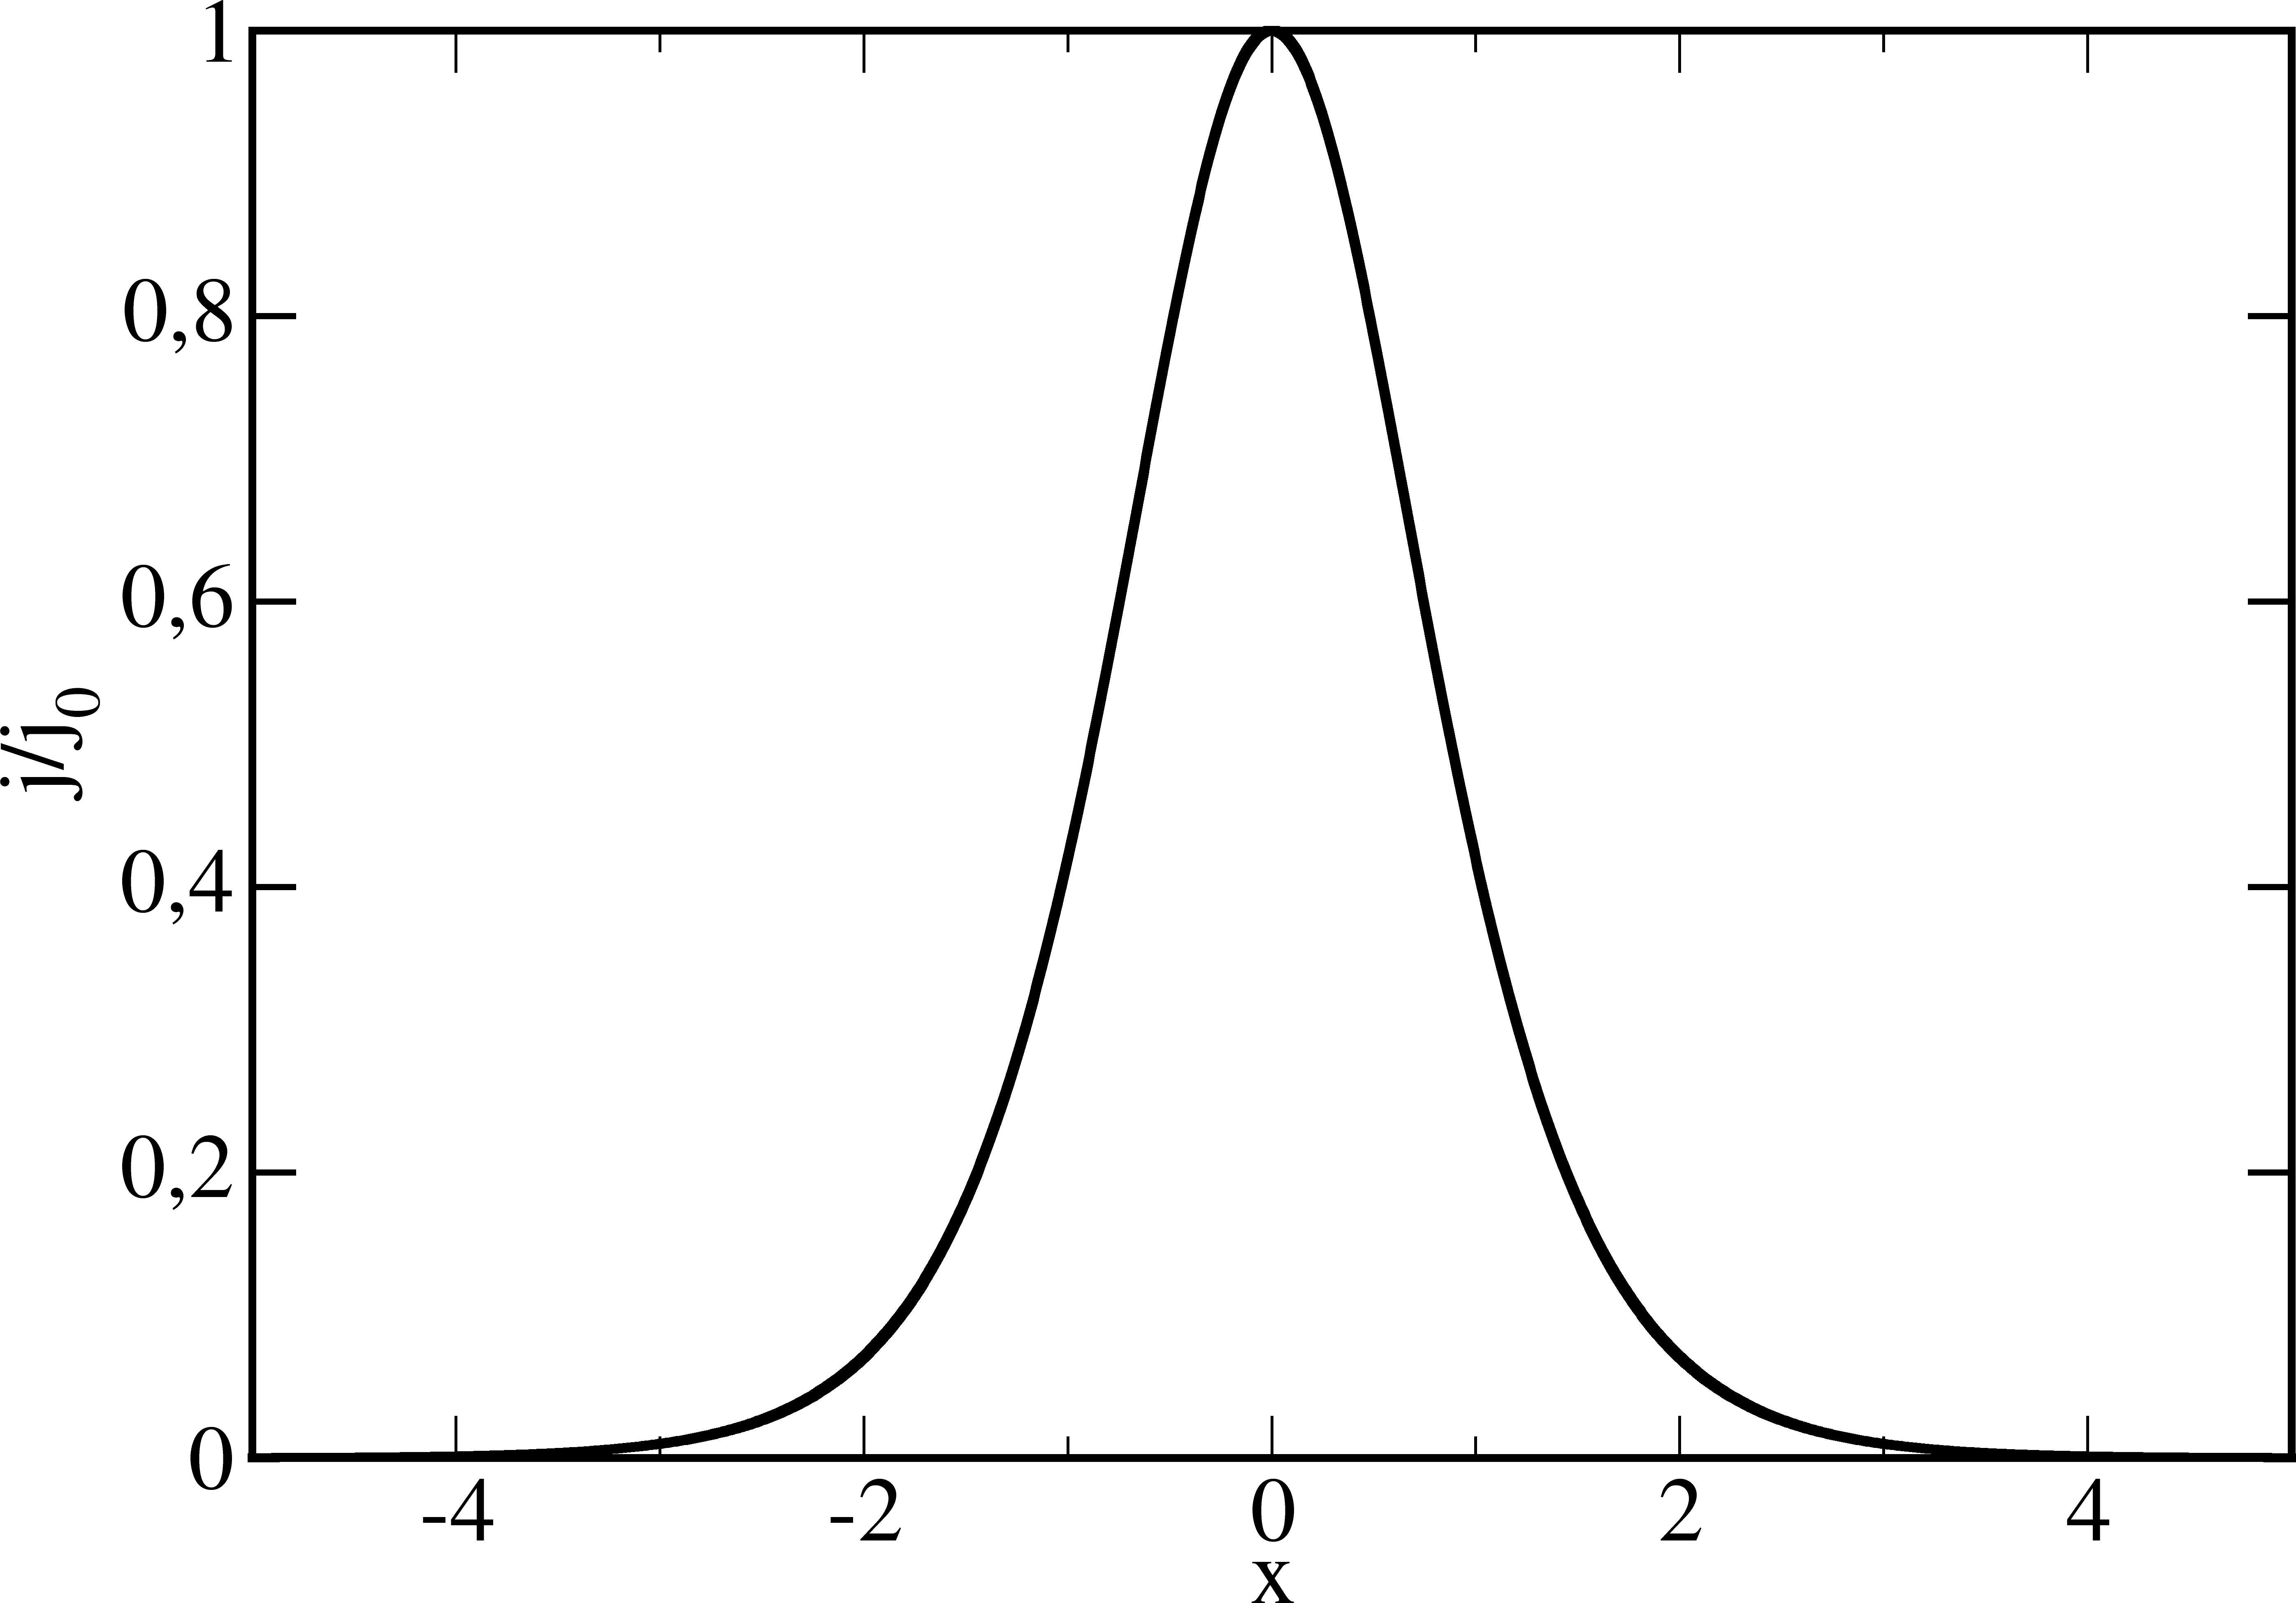
\includegraphics[width=8truecm]{slike/08_soliton.png}
\caption{Prečni profil krajevnega solitona v 2D. Vzdolž koordinate $z$ se profil ohranja.}
\label{fig:soliton}
\end{figure}

Če se vrnemo k izrazu za električno poljsko jakost (enačba~\ref{8.89}), vidimo, da
je parameter $\eta$ nastopa tudi v faznem faktorju. To pomeni, da je od njega odvisna 
tudi konstanta širjenja in s tem fazna hitrost
\index{Soliton!fazna hitrost}
\begin{equation}
v_{f}=\frac{\omega}{k} = \frac{c}{\tilde{n}\left(1+\frac{\eta^{2}}{2k_{0}^{2}}\right)}.
\end{equation}
Fazna hitrost omejenih snopov oziroma solitonov je torej vedno manjša od fazne hitrosti ravnih valov. 
Bolj ko je snop omejen, manjša je fazna hitrost, za velike polmere snopa pa doseže 
limitno vrednost $c_0/\tilde{n}$.

Moč dvodimenzionalnega snopa je enaka integralu
gostote svetlobnega toka (enačba~\ref{8.89a}) po $x$. Integriramo in zapišemo 
\begin{equation}
P_S = \int j_s dx \propto \int |E_S|^2 dx  = 
\frac{2}{\kappa}\,\eta^{2}\int_{-\infty}^{\infty}\frac{dx}
{\cosh^{2}\eta x}=\frac{4\eta}{\kappa}.
\label{eq:solj}
\end{equation}
Moč stacionarnega snopa~\textendash~solitona~\textendash~v dveh dimenzijah je 
torej obratno sorazmerna s širino snopa $1/\eta$. Zato tudi pri poljubno veliki moči 
obstaja stacionarna širina. To je bistvena razlika med obravnavanim dvo- in 
tridimenzionalnim primerom, kjer se snop z nadkritično močjo skrči v singularnost.

\section{Optični solitoni}
\index{Soliton!optični}
V prejšnjem razdelku smo ugotovili, da pojav samozbiranja svetlobnega
snopa lahko izniči širjenje zaradi uklona, tako da ima pri
ustrezni moči snop povsod konstantno širino in obliko. Takim snopom 
smo rekli krajevni solitoni. Povsem podoben pojav poznamo tudi v časovni 
domeni, kjer se pojavijo časovni ali optični solitoni. 

Sunek svetlobe  naj se širi po valovnem vodniku. Ker je lomni količnik
odvisen od frekvence valovanja, se sunek svetlobe podaljšuje. Več o tem bomo spoznali pri 
obravnavi disperzije v optičnih vlaknih (poglavje~\ref{chap:Disperzija}). 
Ob primernih pogojih lahko odvisnost lomnega količnika od intenzitete ravno izniči
odvisnost lomnega količnika od valovne dolžine in sunek
ohranja obliko. Sunkom svetlobe, ki potujejo po sredstvu brez spremembe
oblike, pravimo optični solitoni. Posebej so pomembni v optičnih vlaknih, 
kjer je disperzija izrazita in želimo njen vpliv zaradi učinkovitosti prenosa
informacije čim bolj zmanjšati. 

Pojava optičnih solitonov ni težko pojasniti. Naj na optično nelinearno sredstvo
vpade sunek svetlobe, ki je Gaussove oblike (slika~\ref{fig:optsoliton})
\beq
j(t) = j_0 e^{-t^2/\tau^2}.
\label{08_pulz}
\eeq
Faza takega sunka je 
\beq
\phi (t) = k_o n z - \omega_0 t = k_0 (\tilde{n} + n_2 j)z - \omega_0 t = 
\phi_0 + k_0 n_2 z j - \omega_0 t,
\eeq
frekvenca pa 
\beq
\omega = -\frac{d\phi}{dt} = \omega_0 - k_0 n_2 z \frac{dj}{dt}.
\eeq
Če vstavimo časovno obliko sunka svetlobe (enačba~\ref{08_pulz}), vidimo, da se 
frekvenca takega sunka spreminja s časom
\beq
\omega = \omega_0 + \frac{2k_0 n_2 z j_0}{\tau^2} \, t \, e^{-t^2/\tau^2}.
\eeq
Začetnemu delu sunka (pri $t<0$) se torej frekvenca zmanjša, zadnjemu delu sunka
(pri $t>0$) pa se mu poveča (slika~\ref{fig:optsoliton}). 
Ta pojav spreminjanja frekvence znotraj kratkega sunka imenujemo čričkanje sunkov 
({\it chirping}), \index{Čričkanje} po podobnosti z oglašanjem čričkov.

\begin{figure}[h]
\centering
\def\svgwidth{80truemm} 
\input{slike/08_OpticniSoliton.pdf_tex}
\caption{Zaradi nelinearnega lomnega količnika pride do frekvenčnega premika v sunku svetlobe.}
\label{fig:optsoliton}
\end{figure}
Pri prehodu optičnega sunka z osnovno frekvenco $\omega_0$ se torej različnim delom sunka
frekvenca različno spremeni (slika~\ref{fig:chirp}\,a), začetnemu delu se zmanjša, 
zadnjemu pa poveča. Po drugi strani pa v snoveh poznamo barvno disperzijo, 
kar pomeni, da veljajo za valovanja z različnimi frekvencami različni lomni količniki.
\index{Disperzija} Pojav disperzije je še bolj zapleten pri potovanju sunkov svetlobe,
kar bomo podrobneje obravnavali pri optičnih vlaknih (poglavje~\ref{chap:Disperzija}).
Zaenkrat povejmo le, da je pomemben parameter disperzija grupne hitrosti, ki je sorazmerna
z drugim odvodom lomnega količnika po valovni dolžini 
\beq
D = -\frac{\lambda}{c_0}\frac{d^2n}{d\lambda^2}.
\eeq
Pri določenih pogojih (izbrana snov in določeno frekvenčno območje) 
lahko dosežemo, da potuje del valovanja z večjo valovno dolžino hitreje kot del valovanja
z manjšo valovno dolžino (slika~\ref{fig:chirp}\,b). V tem primeru zadnji del sunka 
dohiteva sprednjega in učinek disperzije ravno izniči učinek nelinearnosti. 
Nastane signal, ki ohranja svojo obliko~\textendash~soliton. 
\begin{figure}[h]
\centering
\def\svgwidth{120truemm} 
\input{slike/08_Chirp.pdf_tex}
\caption{Čričkanje sunkov svetlobe zaradi nelinearnega pojava. Z ustrezno disperzijo lahko
čričkanje izničimo in nastane sunek svetlobe, ki oblike ne spreminja~\textendash~soliton.}
\label{fig:chirp}
\end{figure}

\section{*Izpeljava optičnih solitonov}
\index{Soliton!optični}
Za matematični opis optičnih solitonov izhajamo iz nelinearne 
valovne enačbe (enačba~\ref{8.3}), ki jo zapišemo v skalarni obliki
\begin{equation}
\nabla^{2}E-\frac{n^2}{c_0^{2}}{\frac{\partial^2 E}{\partial t^2}}=
\mu_{0}{\frac{\partial^2P_{\textrm{NL}}}{\partial t^2}},
\end{equation}
pri čemer je 
$P_\textrm{NL}$ nelinearna polarizacija tretjega reda (enačba~\ref{eq:nlin3}).
Namesto v časovni domeni je enačbo prikladnejše reševati v frekvenčni domeni, zato
namesto $E$ in $P_{\mathrm{NL}}$ vpeljemo Fourierevi transformiranki $\tilde{E}$ in $\tilde{P}$.
Sledi
\begin{equation}
\nabla^{2}\tilde{E}+\frac{n^2}{c_0^{2}}\omega^2 \tilde{E}=
- \mu_{0}\omega^2 \tilde{P}.
\end{equation}
Gornjo enačbo rešujemo z nastavkoma
\beq
\tilde{E} = \tilde{A} (z,\omega - \omega_0) e^{ik_0z}\quad \textrm{in} \quad 
\tilde{P} = \tilde{B} (z,\omega - \omega_0) e^{ik_0z},
\eeq
pri čemer je $\omega_0$ osrednja frekvenca svetlobnega sunka in $k_0 = \omega_0 n/c_0$. Vpeljemo še
$\Omega =\omega - \omega_0$
\beq
\left(\frac{\partial^2}{\partial z^2}+k^2\right)\tilde{A}(z,\Omega) e^{ik_0z} =
- \mu_{0}\omega^2 \tilde{B} (z,\Omega) e^{ik_0z}.
\eeq
Da lahko rešimo to enačbo, naredimo nekaj približkov. Ker je $\omega \approx \omega_0$, na desni strani
enačbe nadomestimo frekvenco z osrednjo frekvenco. Poleg tega upoštevamo, da se amplituda 
glede na valovno dolžino le počasi spreminja, zato drugi odvod zanemarimo in 
\beq
2 i k_0 \frac{\partial \tilde{A}}{\partial z} + (k^2-k_0^2) \tilde{A} = - \mu_{0}\omega_0^2 \tilde{B}.
\eeq
Če je disperzija šibka, lahko zapišemo $k^2 - k_0^2$ kot razliko kvadratov, $k(\omega_0 + \Omega)$ pa 
razvijemo v Taylorjevo vrsto okoli osrednje frekvence $\omega_0$ do tretjega člena. Sledi
\beq
k^2 - k_0^2 \approx 2k_0 (k-k_0) \approx 2k_0 (k'\Omega + \frac{1}{2}k''\Omega^2),
\eeq
pri čemer $'$ označuje odvod po frekvenci, in prepišemo enačbo v 
\beq
2 i k_0 \frac{\partial \tilde{A}}{\partial z} + 2k_0(k'\Omega + \frac{1}{2}k''\Omega^2) \tilde{A} 
= - \mu_{0}\omega_0^2 \tilde{B}.
\eeq
Vrnimo se v časovno domeno, tako da naredimo inverzno Fourierevo transformacijo. Naj bo 
$A(z,t)$ kompleksna amplituda električne poljske jakosti in inverzna transformiranka 
funkcije $\tilde{A}(z,\Omega)$, funkcija $B(z,t)$ pa naj bo 
amplituda polarizacije in inverzna transformiranka 
funkcije $\tilde{B}(z,\Omega)$.
Sledi
\begin{equation}
i (\frac{\partial}{\partial z}+\frac{1}{v_{g}}\frac{\partial}{\partial t})A-
\frac{1}{2}\frac{d^{2}k}{d\omega^{2}}\,\frac{\partial^{2}A}{\partial t^{2}}=
-\frac{\mu_0\omega_0^2}{2 k_0}B,
\label{8.93}
\end{equation}
pri čemer smo z $v_g = d\omega/dk = 1/k'$ označili grupno hitrost.
Vpeljimo novo spremenljivko 
\begin{equation}
\tau=t-\frac{z}{v_{g}},
\end{equation}
s katero opišemo obliko sunka $A_S(z,\tau)$, kot ga vidi opazovalec, ki se giblje
z grupno hitrostjo skupaj s sunkom. Uporabimo pravilo verižnega odvajanja in dobimo
\beq
\frac{\partial A}{\partial z} = \frac{\partial A_S}{\partial z} + \frac{\partial A_S}{\partial \tau}
\frac{\partial \tau}{\partial z}
= \frac{\partial A_S}{\partial z} -\frac{1}{v_g} \frac{\partial A_S}{\partial \tau}.
\eeq
Podobno naredimo še za odvod po času $\tau$, ki pa se ne razlikuje od odvoda po času $t$
\beq
\frac{\partial A}{\partial t} = \frac{\partial A_S}{\partial z}\frac{\partial z}{\partial \tau}+
\frac{\partial A_S}{\partial \tau}\frac{\partial \tau}{\partial t} 
= \frac{\partial A_S}{\partial \tau} \qquad \textrm{in} \qquad 
\frac{\partial^2 A}{\partial t^2} = \frac{\partial^2 A_S}{\partial\tau^2}.
\eeq
Vstavimo še amplitudo nelinearne polarizacije (enačba~\ref{eq:ptnl})
\beq
B = \frac{3}{4}\varepsilon_0\chi |A|^2 A.
\eeq
in enačba~(\ref{8.93}) dobi obliko 
\begin{equation}
i\,\frac{\partial A_S}{\partial z}-\frac{1}{2}\frac{d^{2}k}{d\omega^{2}}\,\frac{\partial^{2}A_S}{\partial\tau^{2}}+\kappa\left|A_S\right|^{2}A_S=0,
\label{8.95}
\end{equation}
pri čemer je 
\beq
\kappa = \frac{3\omega_0\chi}{8c_0 \tilde{n}}
\eeq
sorazmeren nelinearnemu lomnemu količniku $n_2$ 
(enačba~\ref{eq:n2}). Enačba~(\ref{8.95}) ni nič drugega kot nelinearna Schr\"odingerjeva 
enačba\index{Nelinearna Schr\"odingerjeva enačba}, ki smo jo 
zapisali že pri izpeljavi krajevnih solitonov~(enačba~\ref{8.84}). Enačbi se razlikujeta v tem, da
ima vlogo prečne koordinate $x$ tukaj čas $\tau$ in rešitve nimajo več konstantnega premera,
ampak imajo konstantno dolžino sunka. Stacionarne rešitve obstajajo le v primeru, kadar je  $d^{2}k/d\omega^{2}<0$ oziroma kadar ima drugi odvod nasprotni predznak od nelinearnega lomnega količnika $n_2$. Kot pri krajevnih solitonih tudi tukaj vpeljemo parameter $\eta$, ki je sorazmeren 
z energijo solitona (enačba~\ref{eq:solj}). Sledi 
\beq
A_S\left(z,\tau\right)=\sqrt{\frac{2}{\kappa}}\eta\frac{e^{i\eta^{2}z}}{{\cosh}\left(\eta \tau 
\sqrt{2\left|\frac{d^{2}\beta}{d\omega^{2}}\right|^{-1}}\right)}\,
\eeq
\begin{equation}
A\left(z,t\right)=\sqrt{\frac{2}{\kappa}}\eta\frac{e^{i\eta^{2}z}}{{\cosh}\left(\eta (t-\frac{z}{v_g}) 
\sqrt{2\left|\frac{d^{2}\beta}{d\omega^{2}}\right|^{-1}}\right)}.
\label{8.96}
\end{equation}
Zapisana je oblika solitona, ki potuje z grupno hitrostjo in pri tem ohranja obliko. Zaradi tega
so solitoni izredno zanimivi za prenos velike gostote informacij na velike razdalje, saj se izognemo
omejitvam zaradi disperzije. 

\begin{remark}
Ena izmed snovi, ki izpolnjuje pogoj, da je $k''$ nasprotnega predznaka kot $n_2$, so kvarčna 
optična vlakna. Pri valovnih dolžinah vidne svetlobe to sicer ne velja, velja pa za 
$\lambda \gtrsim 1,3~\mu$m.
Pogoj je torej izpolnjen pri valovnih dolžinah okoli 1,5~$\mu$m, ki se navadno uporabljajo 
pri prenosu signalov po optičnih vlaknih in signal lahko potuje brez podaljševanja. 
\end{remark}

\section{Optična fazna konjugacija}
\index{Optična fazna konjugacija}
Optična fazna konjugacija je zanimiv in danes tudi praktično pomemben
pojav, pri katerem nastane iz danega valovanja novo valovanje, ki ima enake valovne
fronte, vendar potuje v nasprotni smeri od prvotnega valovanja. Novo valovanje je torej tako,
kot bi začetnemu valovanju obrnili predznak časa in ga ''zavrteli nazaj''. 

Vzemimo optično nelinearno snov, na katero posvetimo z dvema močnima ravnima
snopoma v nasprotnih smereh. To sta črpalna snopa in njuna valovna vektorja 
naj bosta ${\bf k}_{1}$ in ${\bf k}_2 = -{\bf k}_{1}$. Poleg njiju naj na snov vpada
še tretji, signalni snop, ki ni nujno raven val (slika~\ref{08_OPC1}). 
Signalni snop interferira s prvim črpalnim valom in s tem zaradi nelinearnosti 
tretjega reda povzroči modulacijo lomnega količnika, ki je skoraj periodična, če
je signalni val podoben ravnemu valu. Na tej periodični modulaciji se
drugo črpalno valovanje uklanja, pri čemer je uklonjeno valovanje enake oblike
kot signalno, le potuje v nasprotni smeri, ker ima drugo črpalno valovanje
nasprotno smer od prvega. Črpalni valovanji sta seveda enakovredni in ni
mogoče ločiti, s katerim je signalno valovanje interferiralo in katero se
uklanja.
\begin{figure}[h]
\centering
\def\svgwidth{60truemm} 
\input{slike/08_opc1.pdf_tex}
\caption{Optična fazna konjugacija. Dva močna črpalna žarka (modra) vpadata 
na optično nelinearno snov v nasprotnih smereh, vpadni signal (rdeč) pa se odbije v 
smer, iz katere vpada.}
\label{08_OPC1}
\end{figure}
\begin{remark}Pozoren bralec je ugotovil, da je optična fazna konjugacija zelo 
podobna holografiji, le da pri holografiji najprej zapišemo predmetni snop, 
ki ga kasneje reproduciramo, pri fazni konjugaciji pa zapis začetnega valovanja in 
njegova reprodukcija potekata sočasno. 
\end{remark}

Naj se signalno valovanje razširja v smeri $z$. Potem ga zapišemo kot  
\begin{equation}
E_{3}=\mathrm{Re}\left(A_3\left(z\right)\, e^{i\left(kz-\omega t\right)}\right).
\label{8.97}
\end{equation}
V nadaljevanju bomo pokazali, da je novonastalo valovanje sorazmerno
\begin{equation}
E_{4} \propto \mathrm{Re}\left(A_3^{*}\left(z\right)\, e^{i\left(-kz-\omega t\right)}\right).
\label{8.98}
\end{equation}
Zaradi nasprotnega predznaka $k$ potuje nastalo valovanje v obratni smeri od signalnega
valovanja. Poleg tega je kompleksno konjugirana tudi njegova amplituda. To seveda
ne vpliva na obliko valovnih front, saj so te popolnoma enake kot pri signalnem
valovanju. Zaradi lastnosti, da lahko novo valovanje iz signalnega nastane tako,
da krajevni del kompleksno konjugiramo, nastalemu valovanju pravimo fazno
konjugirano valovanje.
\begin{figure}[h!]
\centering
\def\svgwidth{75truemm} 
\input{slike/08_opc2.pdf_tex}
\caption{Primerjava odbojev na navadnem zrcalu (levo) in faznem konjugatorju (desno): odboj ravnega
vala (a), odboj krogelnega valovanja (b) in odboj popačenega vala (c).}
\label{08_OPC2}
\end{figure}

Uporabna posledica fazne konjugacije je prikazana na sliki~(\ref{08_OPC2}).
Najpreprostejši primer je vpad ravnega vala (a), ki se ne odbije po lomnem zakonu (slika levo),
ampak se odbije v smer, iz katere je vpadel na snov (desno). Drugi primer je krogelni val 
ali v približku tudi Gaussov snop (b). Ko vpade na navadno zrcalo (levo), se njegova divergenca
ohranja in se žarek še naprej razširja. Na fazno konjugiranem zrcalu se kroglast val spet
zbere v izvoru (desno). Tretji primer je poljubno sredstvo, ki valovanju doda naključno
fazo, zato po prehodu valovne fronte niso več gladke (c). Ta popačen snop v faznem
konjugatorju generira fazno konjugiran snop, ki potuje v nasprotni smeri
in ima enako nepravilne valovne fronte kot vpadni val. Po prehodu
skozi nepravilno sredstvo se neravnosti valovne fronte izničijo
in nastanejo enake gladke valovne fronte ravnega vala, kot smo jih imeli na začetku. 
To lastnost popravljanja valovne fronte je mogoče 
koristni uporabiti, na primer namesto enega zrcala v laserskem resonatorju.

\section{*Izpeljava optične fazne konjugacije}
Poglejmo podrobneje, kako v nelinearnem sredstvu nastane fazno konjugiran
val. Kot kaže slika~(\ref{08_OPC1}), je celotno polje v nelinearnem
sredstvu vsota štirih valovanj, dveh močnih črpalnih, signalnega in odbitega
\begin{equation}
E=\frac{1}{2}A_{1}e^{i{\bf k}_{1}\cdot{\bf r}-i\omega t}+\frac{1}{2}A_{2}e^{-i{\bf k}_{1}\cdot{\bf r}-
i\omega t}+\frac{1}{2}A_{3}\left(z\right)e^{ikz-i\omega t}+\frac{1}{2}A_{4}
\left(z\right)e^{-ikz-i\omega t}+{\rm k.k.}
\label{8.99}
\end{equation}
S k.k. smo spet označili kompleksno konjugirane člene.  Vsa valovanja naj imajo
enako frekvenco, zaradi enostavnosti še privzemimo, da so enake tudi vse polarizacije.
Račun poenostavimo še s privzetkom, da sta črpalna vala $E_{1}$
in $E_{2}$ dosti močnejša od $E_{3}$ in $E_{4}$, tako da sta njuni
amplitudi konstantni, $E_{3}\left(z\right)$ in $E_{4}\left(z\right)$
pa se le počasi spreminjata.

Vstavimo $E$ v valovno enačbo z nelinearno polarizacijo (enačba~\ref{8.3}), pri čemer
smo časovni odvod že izvrednotili
\begin{equation}
\nabla^{2}E+\epsilon\frac{\omega^{2}}{c_0^{2}}\, 
E=\mu_{0}\frac{\partial^2 P_{\mathrm{NL}}}{\partial t^2}.
\label{8.100}
\end{equation}
Pri tem je $\epsilon\,\omega^{2}/c_0^{2}=k^{2}$, $P_{\textrm{NL}}$ pa je po enačbi~(\ref{eq:nl3P})
enak $P_\mathrm{NL}= \epsilon_{0}\chi^{(3)}E^3$, kjer je $\chi^{(3)} = \chi$
efektivna nelinearna susceptibilnost
za izbrano polarizacijo vseh polj. 

Ker je $E$ zapisan kot vsota osmih različnih členov
(enačba~\ref{8.99}), vsebuje produkt $E^3$ kar 512 členov. Vendar se njihovo število znatno zmanjša, 
če upoštevamo le tiste z enako časovno odvisnostjo oziroma enako frekvenco.
Poleg tega nas ne zanimajo različne kombinacije valovnih vektorjev, ampak k enačbi za $E_{3}$ 
prispevajo le tisti členi s krajevnim faznim faktorjem $\exp(ikz)$, 
k enačbi za $E_4$ pa tisti z $\exp(-ikz)$. Sledi
\begin{eqnarray}
P_{\mathrm{NL}\,3,4} &=& \frac{1}{8}\varepsilon_0\chi 
\left(6 A_1 A_2 A_4^*+ 6A_1 A_1^*A_3 + 6A_2A_2^*A_3 + 3 A_3A_3^*A_3 + 6 A_4 A_4^* A_3^*\right)
e^{i k z - i\omega t} \nonumber\\
&+& 
\left(6 A_1 A_2 A_3^*+6 A_1 A_1^*A_4 + 6A_2A_2^*A_4 + 6 A_3A_3^*A_4 + 3 A_4 A_4 A_4^*\right)
e^{-i k z - i\omega t}.
\end{eqnarray}
Če zanemarimo še člene, v katerih nastopata $A_3$ in $A_4$ v višjih potencah, dobimo
\begin{eqnarray}
P_{\mathrm{NL}\,3,4} &=& \frac{3}{4}\varepsilon_0\chi 
\left( A_1 A_2 A_4^*+ |A_1|^2 A_3 + |A_2|^2 A_3 \right)
e^{i k z - i\omega t} \nonumber\\
&+& 
\left( A_1 A_2 A_3^*+|A_1|^2 A_4 + |A_2|^2A_4 \right)
e^{-i k z - i\omega t}.
\end{eqnarray}
Vstavimo gornji izraz v valovno enačbo~(enačba~\ref{8.100}) in upoštevamo, 
da se $A_i(z)$ le počasi 
spreminja (kar pomeni, da zanemarimo drugi odvod po $z$). Dobimo enačbi 
\beq
i k \frac{dA_3}{dz} = - \frac{3}{4} \mu_0\varepsilon_0 \chi \omega^2 
\left( A_1 A_2 A_4^*+ (|A_1|^2 + |A_2|^2) A_3 \right)
\label{eq:opc1}
\eeq
in 
\beq
-i k \frac{dA_4}{dz} = - \frac{3}{4} \mu_0\varepsilon_0 \chi \omega^2 
\left( A_1 A_2 A_3^*+ (|A_1|^2 + |A_2|^2) A_4 \right).
\label{eq:opc2}
\eeq
Drugi člen na desni že poznamo: opisuje odvisnost lomnega količnika
od intenzitete črpalnih valov, torej optični Kerrov\index{Kerrov pojav!optični}
pojav, in je zato le dodaten prispevek
k fazi. Vpeljimo novi amplitudi, ki se od prejšnjih razlikujeta zgolj v faznem faktorju.
\beq
\tilde{A}_3 = A_3 \exp\left(-i\frac{ 3 \chi \omega}{4 c_0 n}(|A_1|^2 + |A_2|^2) z\right)
\eeq
in 
\beq
\tilde{A}_4 = A_4 \exp\left(i\frac{ 3 \chi \omega}{4 c_0 n}(|A_1|^2 + |A_2|^2)z\right).
\eeq
Ko novi amplitudi vstavimo v diferencialni enačbi~(enačbi~\ref{eq:opc1} in 
\ref{eq:opc2}), se Kerrov prispevek k fazi ravno odšteje
in 
\begin{equation}
\frac{d\tilde{A}_{3}}{dz}=i\frac{ 3 \chi \omega}{4 c_0 n}\,
A_{1}A_{2}\tilde{A}_{4}^{*}
\label{8.104}
\end{equation}
in 
\begin{equation}
\frac{d\tilde{A}_{4}}{dz}=-i\frac{ 3 \chi \omega}{4 c_0 n}\,
A_{1}A_{2}\tilde{A}_{3}^*.
\label{8.105}
\end{equation}
Z vpeljavo sklopitvene konstante 
\begin{equation}
\kappa=\frac{ 3 \chi \omega}{4 c_0 n}A_1 A_2
\label{8.106}
\end{equation}
se enačbi poenostavita v
\beq
\frac{d\tilde{A}_{3}}{dz}=i\kappa \tilde{A}_{4}^{*} \qquad
\textrm{oziroma} \qquad \frac{d\tilde{A}^*_{3}}{dz}=-i\kappa^* \tilde{A}_{4} 
\label{8.107a}
\eeq 
in
\begin{equation}
\frac{d\tilde{A}_{4}}{dz}=-i\kappa \tilde{A}_{3}^*.
\label{8.107}
\end{equation}
Tako smo zelo težaven problem nelinearne valovne enačbe prevedli na linearen
sistem dveh preprostih sklopljenih enačb za amplitudi signalnega in
odbitega vala. Splošni rešitvi sistema enačb~(\ref{8.107a}) in (\ref{8.107}) 
sta 
\begin{eqnarray}
\tilde{A}_3^* \left(z\right) & = & C_{1}\cos(\left|\kappa\right|z)+
C_{2}\sin(\left|\kappa\right|z)
\label{8.108}\\
\tilde{A}_4 \left(z\right) & = & D_{1}\cos(\left|\kappa\right|z)+
D_{2}\sin(\left|\kappa\right|z).
\label{8.108a}
\end{eqnarray}
Z upoštevanjem zveze, ki izhaja neposredno iz diferencialne enačbe 
(enačba~\ref{8.107a}), zapišemo
\beq
C_1 = \frac{i \kappa^*}{|\kappa|}D_2 \qquad
\textrm{in} \qquad 
C_2 = -\frac{i \kappa^*}{|\kappa|}D_1. 
\eeq
Potrebujemo še robne pogoje za obe valovanji. Z leve, pri $z=0$,
poznamo $\tilde{A}_{3}^{*}\left(0\right)$, pri $z=L$ pa ne more biti odbitega
vala in je zato $\tilde{A}_{4}\left(L\right)=0$. S tem lahko določimo konstanti $D_{1}$
in $D_{2}$
\beq
D_2 = -\frac{i|\kappa|}{\kappa^*} \tilde{A}_3^*(0) \qquad
\textrm{in} \qquad 
D_1 = -D_2 \tan(|\kappa|L). 
\eeq
Gornje enačbe združimo in lahko zapišemo amplitudi znotraj nelinearne snovi
\begin{eqnarray}
\tilde{A}_{3}\left(z\right) & = & \tilde{A}_3(0)
\frac{\cos\left(|\kappa|(L-z)\right)}{\cos\left(|\kappa|L\right)}\\
\tilde{A}_{4}\left(z\right) & = & \tilde{A}_3^*(0)\frac{i \kappa}{|\kappa|}
\frac{\sin\left(|\kappa|(L-z)\right)}{\cos\left(|\kappa|L\right)}
\label{8.109}
\nonumber 
\end{eqnarray}
Izračunajmo še amplitudi odbitega in prepuščenega vala. Amplituda odbitega vala 
pri $z=0$ je 
\boxeq{8.110}{
\tilde{A}_{4}(0)  =  \tilde{A}_3^*(0)\frac{i \kappa}{|\kappa|}
\tan \left(|\kappa|L\right),
}
amplituda prepuščenega pri $z = L$ pa
\boxeq{8.110a}{
\tilde{A}_{3}(L)  =  \frac{\tilde{A}_3^*(0)}{
\cos \left(|\kappa|L\right)}.
}
Oglejmo si gornja rezultata podrobneje. Vidimo, da je odbiti val sorazmeren 
kompleksno konjugirani amplitudi vpadnega vala, kar smo omenili že v prejšnjem
razdelku. Poleg konjugirane amplitude ima tudi natanko nasproten valovni vektor, 
zato tudi ime fazno konjugiran val. Zanimiva je tudi njegova velikost. Ker 
je lahko $\tan\left(|\kappa|L\right)>1$, je odbit val lahko močnejši od vpadnega.
To ojačanje odbitega vala gre seveda na račun moči črpalnih
valov. V našem računu bi lahko amplituda odbite svetlobe narasla proti neskončnosti, 
vendar ne smemo pozabiti, ta zapisane enačbe takrat niso več veljavne, ker smo privzeli, 
da sta signalni in odbiti žarek precej šibkejša od črpalnih.

Poglejmo še prepuščeni žarek. Ker je $\cos(x)\leq1$, je amplituda prepuščenega
žarka vedno večja od amplitude vpadnega. To pomeni, da smo na račun črpalnih žarkov
dobili prepustnost, ki je vedno večja od $100~\%$, in odbojnost, ki je lahko 
večja od $100~\%$.

Doslej smo predpostavili, da je vpadni signal ravni val. Če je njegova
amplituda odvisna še od prečne koordinate, ga lahko razvijemo po ravnih
valovih in zgoraj izpeljana enačba~(\ref{8.110}) velja za vsako komponento posebej. 
Odbite komponente so sorazmerne s konjugiranimi komponentami signalnega valovanja
z nasprotnim valovnim vektorjem in dajo skupaj valovno fronto enake
oblike kot pri signalnem valovanju, le giblje se v nasprotni smeri, kot
smo opisali že na začetku razdelka.

\begin{remark}
Omenili smo že, da se fazno konjugirana zrcala lahko uporabljajo v laserjih, da
izničimo popačenje Gaussovega snopa. Drug primer uporabe je pri optični astronomiji
ali optičnih komunikacijah skozi atmosfero. Naključne spremembe gostote v atmosferi
signalu dodajo naključni fazni premik, ki signal popači. Če se signal odbije od zrcala nazaj
proti izvoru, bo torej dvakratno popačen. Če pa se odbije od fazno konjugiranega zrcala, 
se bo vpliv nehomogenosti atmosfere ravno izničil in na prenos signala ne bo vplival, poleg
tega pa bo šibek signal še dodatno ojačan. 
\end{remark}
%Končano

%-------------------------------------------------------------------------------
%	CHAPTER 9
%-------------------------------------------------------------------------------

\chapterimage{AOModulator.jpg} % Chapter heading image

\chapter{Modulacija svetlobe}

V optičnih napravah pogosto želimo spreminjati lastnosti svetlobnega
valovanja. Tak primer smo že spoznali pri obravnavi laserja, kjer za 
preklop dobrote potrebujemo element, ki hitro spreminja prepustnost. 
Še pomembnejša je modulacija valovanja pri optičnem prenosu informacij.

Svetlobno valovanje lahko moduliramo na več načinov. Z ustreznim moduliranjem
lomnega količnika lahko valovanju spreminjamo amplitudo\index{Elektro-optična modulacija!amplitudna} 
ali frekvenco oziroma fazo\index{Elektro-optična modulacija!frekvenčna}
\index{Elektro-optična modulacija!fazna}. 
\begin{figure}[h]
\centering
\def\svgwidth{140truemm} 
\input{slike/09_AMFM.pdf_tex}
\caption{Amplitudno (levo) in fazno oziroma frekvenčno moduliran signal (desno)
}
\label{fig:amfm}
\end{figure}

Delovanje optičnih modulatorjev temelji na različnih pojavih. V tem poglavju bomo 
podrobneje spoznali dva načina, to sta elektro-optični in elasto- oziroma akusto-optični pojav. 
Pri prvem pride do spremembe lomnega količnika snovi pod vplivom zunanjega električnega polja, 
pri drugem pa zaradi mehanske deformacije. Kadar mehansko deformacijo povzroči zvočno valovanje, 
takim modulatorjem pravimo akusto-optični. Na koncu bomo spoznali poseben zelo pomemben 
primer elektro-optičnih modulatorjev na osnovi tekočih kristalov.

\section{Elektro-optični pojav}
Elektro-optični pojav\index{Elektro-optični pojav} opisuje spremembe optičnih lastnosti 
snovi (dielektričnosti in lomnega količnika) pod vplivom zunanjega električnega polja. 
Omejimo se na statično zunanje polje oziroma
na polje, katerega frekvenca je bistveno manjša od optične frekvence. Omejitev na nizko 
frekvenco je potrebna zato, da optično polje še lahko obravnavamo linearno. 
Kako je v nasprotnem primeru, ko je frekvenca polja primerljiva z optično frekvenco, 
smo na široko obravnavali v poglavju o nelinearni optiki (poglavje~\ref{chap:NLO}).

Namesto dielektričnega tenzorja\index{Dielektričnost!inverzna} 
navadno vpeljemo inverzni dielektrični tenzor
\beq
\underline{b}=\underline{\epsilon}^{-1}.
\eeq
Izračunajmo zvezo med spremembo inverznega tenzorja $\delta b_{ij}$ 
in spremembo dielektričnega tenzorja $\delta \varepsilon_{ij}$. 
Če so spremembe majhne, velja 
\begin{equation}
\underline{\varepsilon} = \underline{\tilde{\varepsilon}} + \delta \underline{\varepsilon}=
(\underline{b}+\delta \underline{b})^{-1}=\left(\underline{b}(1+\underline{b}^{-1}
\delta \underline{b})\right)^{-1}=(1+\underline{b}^{-1}\delta \underline{b})^{-1}\underline{b}^{-1}
\approx \underline{b}^{-1}-\underline{b}^{-1}\delta \underline{b}\, \underline{b}^{-1}.
\label{7.2}
\end{equation}
Sprememba dielektričnega tenzorja je tako
\beq
 \delta \underline{\varepsilon}= -\underline{b}^{-1}\delta \underline{b}\, \underline{b}^{-1}
 = -\underline{\tilde{\varepsilon}}\, \delta \underline{b}\, \underline{\tilde{\varepsilon}}.
\eeq
Če je nemoten dielektrični tenzor $\underline{\tilde{\varepsilon}}$ diagonalen, velja
\begin{equation}
\delta\epsilon_{ij}=-\tilde{\epsilon}_{ik}\delta b_{kl}\tilde{\epsilon}_{lj}
=-\tilde{\epsilon}_{ii}\tilde{\epsilon}_{jj}\delta b_{ij}.
\label{7.3}
\end{equation}

Pri elektro-optičnem pojavu so spremembe tenzorja dielektričnosti zaradi vpliva zunanjega polja razmeroma 
majhne. Spremembo komponente $\delta b_{ij}$ lahko zato zapišemo kot potenčno vrsto zunanjega polja $E$, 
pri čemer upoštevajmo zgolj prva dva člena v razvoju
\boxeq{7.1}{
\delta b_{ij}=r_{ijk}E_{k}+q_{ijkl}E_{k}E_{l}.
}
Prvi člen, linearno sorazmeren zunanjem polju, opisuje linearni elektro-optični
ali Pockelsov\index{Pockelsov pojav} pojav\footnote{Nemški fizik Friedrich Carl Alwin Pockels, 1865--1913.}. 
Tenzor tretjega ranga $r_{ijk}$, ki je lastnost snovi, imenujemo elektro-optični 
tenzor\index{Elektro-optični tenzor}
ali tudi Pockelsov tenzor\index{Pockelsov tenzor|see {Elektro-optični tenzor}}. 
Pockelsov tenzor je različen od nič v snoveh brez centra inverzije, značilne vrednosti Pockelsovega
tenzorja pa so okoli $r \sim 10^{-12} - 10^{-10}$~m/V,

Kvadratnemu elektro-optičnemu pojavu pravimo Kerrov\index{Kerrov pojav}
pojav\footnote{Škotski fizik John Kerr, 1824--1907.}, tenzorju $q_{ijkl}$ pa Kerrov tenzor\index{Kerrov tenzor}. 
Kerrov pojav je praviloma precej šibkejši od Pockelsovega, vendar je različen od nič v vseh snoveh, ne glede na
njihove simetrijske lastnosti, torej tudi v tekočinah. 
Značilna vrednost Kerrovega tenzorja je $q \sim 10^{-24}$~m$^2$/V$^2$. Navadno ločimo dva primera Kerrovega
pojava: Kerrov elektro-optični pojav pri zunanjih poljih z nizko frekvenco, in optični Kerrov pojav, ki smo 
ga podrobneje spoznali pri obravnavi nelinearnih optičnih pojavov (poglavje~\ref{OKP}).

Za uporabo trdnih kristalov je pomemben
predvsem linearni člen, zato se bomo osredotočili le nanj in zapisali
\boxeq{eq:Pockels}{
\delta b_{ij}=r_{ijk}E_{k}. 
}

\subsection*{Elektro-optični ali Pockelsov tenzor}
Simetrija snovi pomembno vpliva na obliko tenzorjev, ki opisujejo njene lastnosti.
Pockelsov tenzor $r$ je tenzor tretjega ranga, zato je lahko različen
od nič le v kristalih brez centra inverzije. 
Simetrija kristala tudi v primeru, ko ni centra inverzije, močno
zmanjša število neodvisnih komponent $r_{ijk}$. 

Ker je inverzni dielektrični tenzor $b$ simetričen, je v prvih dveh indeksih simetričen
tudi Pockelsov tenzor
\beq
r_{ijk} = r_{jik}.
\eeq
V najmanj simetričnem primeru triklinskega kristala ima tako namesto 27 zgolj 
18 neodvisnih komponent, v kristalih z višjo simetrijo pa še manj. 

Podobno kot pri nelinearni susceptibilnosti (poglavje~\ref{Chap:Chi}) 
tudi elektro-optični tenzor pogosto zapišemo le z dvema komponentama. 
Prva dva indeksa, v katerih je $r_{ijk}$ simetričen, združimo
v enega z vrednostmi od 1 do 6 po dogovoru $xx=1$, $yy=2$, $zz=3$,
$yz=4$, $zx=5$ in $xy=6$. Tako postane $r_{ijk}$ matrika velikosti
$6\times3$, simetrični tenzor drugega ranga $b_{ij}$ pa šestdimenzionalen
vektor.

\begin{definition}
Naj bo $Q$ transformacijska matrika za dano simetrijsko operacijo. Potem za tenzorje
tretjega ranga velja
\beq
r_{ijk} = Q_{ip}Q_{jq}Q_{kr}r_{pqr}.
\eeq
Zapiši transformacijsko matriko $Q$ za vrtenje okoli osi $z$ za $\pi/2$ in pokaži, da so
v primeru štirištevne simetrije od nič različne le komponente $r_{xxz}=r_{yyz}, r_{zzz}, 
r_{yzx}=-r_{xzy}$ in $r_{xzx}=r_{yzy}$. Razmisli in izračunaj, kakšen bi bil tenzor $r$, če bi 
štirištevni simetriji dodali še zrcaljenje čez ravnino $xy$.
\end{definition}

Nekaj primerov Pockelsovih tenzorjev pri različnih kristalnih simetrijah
je podanih v tabeli~(\ref{table:Pockels}).

\begin{table}[h!]
 \centering
\begin{tabular}{|c|c|c|c|} \hline  
      Kristal & Grupa & Neničelne komponente tenzorja $r$ & Vrednost ($10^{-12}$~m/V)\\ \hline
      BaTiO$_3$\index{BaTiO$_3$} & 4mm & $r_{xzx} = r_{yzy} = r_{zxx} = r_{zyy} = 
      r_{51} = r_{42}$  &
	    (pri 1,55~$\mu$m) $r_{51} = 800$ \\
	      & & $r_{xxz} = r_{yyz} = r_{13} = r_{23}$ &  $r_{13} = 8$ \\
	      & & $r_{zzz} = r_{33}$ & $r_{33} = 28$ \\ \hline
      KDP\index{KDP} & 
      $\overline{4}$2m & $r_{yzx} = r_{zyx} = r_{xzy} = r_{zxy} = r_{41} = r_{52}$  &
	    $r_{41} = 8,77$ \\
	    & & $r_{xyz} = r_{yxz} = r_{63}$ &  $r_{63} = -10,3$ \\ \hline
      GaAs\index{GaAs}\index{ZnTe} &  $\overline{4}$3m&
	  $r_{yzx} = r_{zyx} = r_{xzy} = r_{zxy} = r_{xyz} = r_{yxz}$  & (pri 10,6~$\mu$m) $r_{41} = 1,5$ \\
	ZnTe  & &   $= r_{41} = r_{52}=r_{63}$  &(pri 3,4~$\mu$m) $r_{41} = 4,2$ 
	    \\ \hline
      LiNbO$_3$\index{LiNbO$_3$} & 3m & $r_{xzx} = r_{zxx} = r_{yzy} = r_{zyy} = r_{51} = r_{42}$  &
	    $r_{51} = 32,6$ \\
	     & & $r_{xxz} = r_{yyz} = r_{13} = r_{23}$ &  $r_{13} = 9,6$ \\
	      & & $r_{zzz} = r_{33}$ & $r_{33} = 30,9$ \\
	    & &  $r_{yyy} = - r_{xxy} = -r_{xyx} = -r_{yxx}  = $ & \\
	    & &  $=r_{22} =  -r_{12} =-r_{61} $  &
	    $r_{22}  = 6,8$ \\
\hline 
\end{tabular}
  \caption{Koeficienti Pockelsovega tenzorja za nekaj izbranih snovi. Če ni navedeno drugače, veljajo
  vrednosti pri valovni dolžini okoli 600~nm.}
\label{table:Pockels}
\end{table}

\begin{remark}
Komponente elektro-optičnega tenzorja zaradi nazornosti pogosto ponazarjamo grafično. V matriki $6\times 3$
s piko označimo komponente, ki so enake nič, s polnim krožcem neničelne komponente, povezava med 
komponentami pomeni njihovo enakost, prazen krožec in črtkana črta pa označujeta 
neničelno komponento nasprotnega predznaka. Kot primer sta podana prikaza tenzorjev za 
GaAs (levo) in LiNbO$_3$ (desno).
\begin{figure}[h!]
\centering
\def\svgwidth{20truemm} 
\input{slike/09_tensor.pdf_tex}\qquad \qquad
\def\svgwidth{20truemm} 
\input{slike/09_tensor2.pdf_tex}
\end{figure}
\end{remark}

\section{Longitudinalna modulacija}
Poglejmo podrobneje, kako električno polje spremeni optične lastnosti 
elektro-optičnega kristala in kako to vpliva na svetlobo, ki potuje skozi tak kristal.
Navadno se uporabljajo kristali, ki so dvolomni že brez zunanjega polja. 
Kot primer vzemimo kristal KH$_{2}$PO$_{4}$ (KDP)\index{KDP}, ki ima tetragonalno 
simetrijo ($\bar{4}2m$). Kot razberemo iz tabele~(\ref{table:Pockels}) ima 
elektro-optični tenzor dve neodvisni komponenti: $r_{41} = r_{52}=8,77 \times 10^{-12}$~m/V
in $r_{63}= -10,3 \times 10^{-12}$~m/V.

Kristal naj bo odrezan po kristalografskih oseh, svetloba naj skozi kristal potuje 
v smeri optične osi, to je smeri $z$, v isti smeri pa na kristal priključimo
polje $E_z$. Ker je smer električnega polja vzporedna s smerjo širjenja svetlobe, taki 
postavitvi pravimo longitudinalna in pojavu longitudinalna 
modulacija.\index{Elektro-optična modulacija!longitudinalna} 
\begin{figure}[h]
\centering
\def\svgwidth{80truemm} 
\input{slike/09_AMshema.pdf_tex}
\caption{Shema longitudinalne modulacije signala. Ker je polje priključeno v smeri
potovanja svetlobe, morata biti elektrodi transparentni. Z uporabo polarizatorja in 
analizatorja sestavimo amplitudni modulator (glej poglavje~\ref{chap:ampmod}).}
\label{fig:amshema}
\end{figure}

Inverzni tenzor dielektričnosti v odsotnosti zunanjega polja zapišemo kot
\beq
\underline{\tilde{b}} = 
\left[\begin{array}{ccc}
1/n_o^2 & 0& 0\\
0 & 1/n_o^2& 0\\
0 & 0&  1/n_e^2
\end{array}\right],
\label{7.8}
\eeq
pri čemer sta $n_o$ in $n_e$ redni in izredni lomni količnik. Ko priključimo 
polje, se tenzor dielektričnosti spremeni zaradi Pockelsovega pojava. Sprememba
inverznega tenzorja dielektričnosti je po enačbi~(\ref{eq:Pockels})
\begin{align}
\delta b_{xx} & =r_{xxx}E_x + r_{xxy}E_y + r_{xxz}E_z = 0,\nonumber \\
\delta b_{xy} & = \delta b_{yx} = r_{xyx}E_x + r_{xyy}E_y + r_{xyz}E_z = r_{63}E_z,\nonumber\\
\delta b_{xz} & = \delta b_{zx} =r_{xzz}E_z = 0,\nonumber\\
\delta b_{yy} & =r_{yyz}E_z = 0,\nonumber\\
\delta b_{yz} & = \delta b_{zy} =r_{yzz}E_z = 0,\nonumber\\
\delta b_{zz} & =r_{zzz}E_z = 0.
\end{align}
Vidimo, da je večina členov enaka nič, se pa zaradi zunanjega električnega
polja v smeri $z$ pojavi izvendiagonalna komponenta 
\beq
\underline{b} = 
\left[\begin{array}{ccc}
1/n_o^2 & 0& 0\\
0 & 1/n_o^2 & 0\\
0 & 0& 1/n_e^2
\end{array}\right] + \left[\begin{array}{ccc}
 0& r_{63}E_z& 0\\
r_{63}E_z & 0 & 0\\
0 & 0&  0
\end{array}\right] = \left[\begin{array}{ccc}
1/n_o^2 & r_{63}E_z& 0\\
r_{63}E_z& 1/n_o^2 & 0\\
0 & 0&  1/n_e^2
\end{array}\right].
\label{7.8a}
\eeq
Če želimo izračunati, kako se po kristalu pod napetostjo širi vpadni svetlobni
snop, moramo gornji dielektrični tenzor diagonalizirati. Lastne vrednosti novega tenzorja
in pripadajoče nove lastne osi so
\begin{align}
\lambda_1 &= \frac{1}{n_o^2}+ r_{63}E_z \quad \mathrm{in} \quad \mathbf{e}_1 = \frac{1}{\sqrt{2}}(1,1,0)\\
\lambda_2 &= \frac{1}{n_o^2}- r_{63}E_z \quad \mathrm{in} \quad \mathbf{e}_2 = \frac{1}{\sqrt{2}}(-1,1,0)\\
\lambda_3 &= \frac{1}{n_e^2} \quad \mathrm{in} \quad \mathbf{e}_3 = (0,0,1).
\end{align}
Vidimo, da so nove lastne osi zasukane za kot $45~^\circ$ glede na prvotne osi sistema.
V novem koordinatnem sistemu je inverzni dielektrični tenzor diagonalen in enak
\beq
\underline{b} = 
\left[\begin{array}{ccc}
1/n_o^2 + r_{63}E_z& 0& 0\\
0 & 1/n_o^2 - r_{63}E_z& 0\\
0 & 0& 1/n_e^2
\end{array}\right].
\eeq
\begin{figure}[h]
\centering
\def\svgwidth{60truemm} 
\input{slike/09_AMindikatrisa.pdf_tex}
\caption{Optično enoosni kristal postane pod napetostjo dvoosen. Indikatrisa, ki je pravokotno
na optično os brez polja krožnica, se pod vplivom napetosti spremeni v elipso. }
\label{fig:amn}
\end{figure}

Spomnimo se, da potuje svetloba skozi kristal vzdolž osi $z$. Brez zunanjega električnega
polja je kristal enoosen z optično osjo v smeri $z$. Lomni količnik je torej neodvisen od
polarizacije vpadnega valovanja in je enak $n_o$. Ko priključimo polje, postane kristal
optično dvoosen, saj so vse tri lastne vrednosti tenzorja dielektričnosti različne. Za žarek, 
ki potuje vzdolž osi $z$, torej obstajata dve lastni smeri $x'$ in $y'$ z ustreznima
novima lastnima količnikoma, ki ju izrazimo kot
\beq
\frac{1}{n_{x'}^2} = \frac{1}{n_o^2}+ r_{63}E_z \quad \mathrm{in} \quad 
\frac{1}{n_{y'}^2} = \frac{1}{n_o^2}- r_{63}E_z. 
\eeq
Kadar polarizacija vpadnega valovanja ne sovpada z novimi lastnimi osmi $x'$ ali $y'$, je 
svetloba po preletu kristala v splošnem eliptično polarizirana.

Za vsa eksperimentalno dosegljiva polja velja, da je $rE\ll1/n^2$, 
zato lahko gornja izraza razvijemo za majhne popravke
\beq
n_{x'} = \sqrt{\frac{n_o^2}{1+ n_o^2 r_{63}E_z}} \approx n_o \sqrt{1- n_o^2 r_{63}E_z}.
\eeq
Sledi
\boxeq{EOnx}{
n_{x'}\approx n_o - \frac{1}{2}n_o^3 r_{63}E_z.
}
Podobno izpeljemo še za drugo lastno vrednost
\boxeq{EOny}{
n_{y'}\approx n_o + \frac{1}{2}n_o^3 r_{63}E_z.
}
Različni lastni polarizaciji potujeta vzdolž osi $z$ z različnima hitrostma. Ko 
prepotujeta dolžino kristala $L$, pride med njima do fazne razlike
\beq
\Delta \phi = k_0 n_{y'} L - k_0 n_{x'} L = \frac{\omega}{c_0}L 
n_o^3 r_{63}E_z.
\label{phiAM}
\eeq
Prelet kristala torej doda vpadnemu valovanju fazni zamik, ki je odvisen od električne poljske
jakosti $E_z$. 

Vpeljemo še karakteristično napetost $U_\pi$, pri kateri je dodatna \index{$\pi$-napetost}
fazna razlika enaka $\pi$ in kristal deluje kot ploščica $\lambda/2$\index{Ploščica $\lambda/2$}
\boxeq{UpiL}{
U_\pi = \frac{\pi c_o}{\omega n_o^3 r_{63}} = \frac{\lambda}{2 n_o^3 r_{63}}.
}
Za kristal KDP je $\pi$-vrednost napetosti pri valovni dolžini $633$~nm okoli  $9000$~V. 
Izračunana napetost je precej velika. Velike delovne napetosti
so značilne za kristalne elektro-optične modulatorje in so njihova
glavna pomanjkljivost. 

\section{Transverzalna modulacija}
\index{Elektro-optična modulacija!transverzalna}
Iz praktičnih razlogov je navadno preprosteje priključiti električno polje v smeri, ki 
je pravokotna na smer širjenja svetlobe. Taki postavitvi pravimo transverzalna in pojavu
transverzalna modulacija\index{Elektro-optična modulacija!transverzalna}.

Tudi to postavitev obravnavajmo na primeru. Za zgled vzemimo kristal LiNbO$_3$, ki 
ima trigonalno simetrijo (3m) in po tabeli~(\ref{table:Pockels}) štiri 
neodvisne komponente: $r_{51}=r_{42}, r_{13}=r_{23}, r_{33}$ in $r_{22}=-r_{12}=-r_{61}$.

\begin{figure}[h]
\centering
\def\svgwidth{80truemm} 
\input{slike/09_TMshema.pdf_tex}
\caption{Shema transverzalne modulacije signala}
\label{fig:tmshema}
\end{figure}
\pagebreak
Naj se svetloba širi vzdolž osi $z$, ki je hkrati tudi optična os, 
električno polje pa priključimo v smeri $y$ (slika~\ref{fig:tmshema}). 
Krajši račun pokaže, da je inverzni dielektrični tenzor pod vplivom polja enak
\beq
\underline{b} = 
 \left[\begin{array}{ccc}
1/n_o^2  -r_{22}E_y& 0& 0\\
0& 1/n_o^2+r_{22}E_y& r_{51}E_y\\
0 & r_{51}E_y&  1/n_e^2
\end{array}\right].
\label{7.8b}
\eeq
Tudi v tem primeru tenzor diagonaliziramo in poiščemo nove lastne vrednosti.
Ob privzetku, da je sprememba zaradi električnega polja majhna ($rE\ll1$),
so nove lastne vrednosti enake
\begin{align}
\lambda_1 &\approx \frac{1}{n_o^2}-r_{22}E_y \\
\lambda_2 &\approx \frac{1}{n_o^2}+ r_{22}E_y \\
\lambda_3 &\approx \frac{1}{n_e^2},
\end{align}
kar ustreza lomnim količnikom 
\begin{align}
n_{x'} &\approx n_o(1+\frac{1}{2}n_o^2r_{22}E_y)\\
n_{y'} &\approx n_o(1-\frac{1}{2}n_o^2r_{22}E_y)\\
n_z' &\approx n_e.
\end{align}
Kako pa je z novimi lastnimi osmi? Hitro ugotovimo, da se tudi pri 
priključenem polju os $x$ ohranja. Pojavi se torej zasuk okoli osi $x$,
ki ga označimo s kotom $\vartheta$. Račun pokaže, da je za smiselne
vrednosti električnega polja ta kot zelo majhen ($\vartheta~
\approx~r_{51}E_y/(1/n_o^2-1/n_e^2) \sim~1$~mrad),
tako da lahko v približku rečemo, da se lastne osi ohranjajo. 

Če potuje svetloba vzdolž osi $z$, sta torej lomna količnika za 
polarizaciji v smeri $x$ in $y$ približno enaka $n_{x'}$ in $n_{y'}$, fazna razlika med 
polarizacijama po preletu kristala z dolžino $L$ pa je 
\beq
\Delta \phi = k_0 n_{y'} L - k_0 n_{x'} L = \frac{\omega}{c_0}L 
n_o^3 r_{22}E_y.
\label{fazaTM}
\eeq
Karakteristična $\pi$-napetost \index{$\pi$-napetost}je tako
\boxeq{UpiT}{
U_\pi = \frac{\lambda d}{2 Ln_o^3 r_{22}},
}
pri čemer moramo ločiti med $L$, ki je dolžina kristala v smeri $z$, in $d$, ki je  
širina v prečni smeri v kateri priključimo napetost. 
Za izbran kristal ($d=5$~mm, $L=1$~cm) je $\pi$-vrednost 
napetosti pri valovni dolžini $633$~nm okoli $2000$~V. 

\begin{remark}
Transverzalno modulacijo lahko dosežemo tudi tako, da se žarek širi vzdolž 
osi $y$, električno polje pa priključimo vzdolž optične osi $z$.
V tem primeru se lastne osi ohranijo in kristal ostane optično enoosen. Vendar 
pa ima tudi ta rešitev določene slabosti. Ker je kristal že sam po sebi dvolomen\index{Dvolomnost}, 
povzroči zunanje polje le majhno dodatno fazno razliko, zato je najbolje, če je dolžina 
kristala taka, da velja $k_{0}L(n_{o}-n_{e})=2N\pi$. Pri tem pa nastopi težava. 
Pogoj je lahko zaradi temperaturnega raztezanja in odvisnosti lomnih količnikov od temperature
izpolnjen le pri eni temperaturi, poleg tega se mora svetloba širiti natančno v smeri $y$.
Zato dvolomnost nemotenega kristala navadno kompenziramo, tako da postavimo 
dva enako dolga kristala zapored, pri čemer sta optični
osi med seboj pravokotni, modulacijska napetost na drugem kristalu pa ima
nasproten predznak. Tedaj se fazna razlika med obema polarizacijama zaradi 
naravne dvolomnosti odšteje, zaradi modulacijske napetosti pa sešteje.
\end{remark}

\section{Amplitudna modulacija}
\label{chap:ampmod}
\index{Elektro-optična modulacija!amplitudna}
Poglejmo, kako lahko elektro-optični pojav izkoristimo za modulacijo
amplitude svetlobnega snopa. Pod vplivom polja pride v kristalu do
faznega zamika med polarizacijama, ki je sorazmeren napetosti 
(enačbi~\ref{phiAM} in \ref{fazaTM}).
Če za tak kristal postavimo analizator, lahko z napetostjo spreminjamo 
prepuščeno moč svetlobe -- amplitudno moduliramo signal.

Vrnimo se k longitudinalni\index{Elektro-optična modulacija!longitudinalna}
modulaciji (slika~\ref{fig:amshema}).
Naj bo vpadna električna poljska jakost $E_0$ polarizirana v smeri $y$. 
Ko priključimo napetost, os $y$ ni več lastna os, ampak sta lastni osi zasukani 
za kot $45~^\circ$ glede na prvotni lastni osi (slika~\ref{fig:amn}). Vpadno 
valovanje razstavimo na komponenti $x'$ in $y'$
\beq
\mathbf{E}_0 = E_0\, \mathbf{e}_y = \frac{E_0}{\sqrt{2}}\left(\mathbf{e}_{x'} + \mathbf{e}_{y'}\right).
\eeq
Po prehodu skozi kristal pride med njima do fazne razlike $\Delta \phi$ 
(enačba~\ref{phiAM}), zato je polje $\mathbf{E}_1$ ob izstopu iz kristala
\beq
\mathbf{E}_1 = \frac{E_0}{\sqrt{2}}\left(e^{ik_0 n_{x'}L}\mathbf{e}_{x'} + 
e^{ik_0 n_{y'}L}\mathbf{e}_{y'}\right)
= \frac{E_0}{\sqrt{2}}e^{ik_0 n_{x'}L}\left(\mathbf{e}_{x'} + 
e^{i\Delta\phi}\mathbf{e}_{y'}\right).
\eeq
Analizator na izhodni strani je obrnjen v smeri $x$, to je pravokotno
na smer vpadne polarizacije, in prepusti le projekcijo obeh lastnih polarizacij
na os $x$
\begin{equation}
\mathbf{E}_2= \mathbf{E}_1 \cdot \mathbf{e}_x = 
\frac{E_0}{\sqrt{2}}e^{ik_0 n_{x'}L}
\left(\frac{1}{\sqrt{2}} -\frac{1}{\sqrt{2}} e^{i\Delta\phi}\right)\mathbf{e}_x .
\label{7.16}
\end{equation}
Gostota prepuščenega svetlobnega toka ob vpadnem toku $j_0$ je tako 
\begin{equation}
j=\frac{1}{4}j_{0}\left|1-e^{i\Delta\phi}\right|^{2}=\frac{1}{2}j_{0}(1-\cos\Delta\phi).
\label{7.17}
\end{equation}
Preoblikujemo izraz in zapišemo prepustnost takega modulatorja ob upoštevanju 
enačbe~(\ref{phiAM})
\boxeq{AMfinal}{
T = \frac{j}{j_0} = \sin\left(\frac{\Delta\phi}{2}\right)^2 = 
\sin\left(\frac{\pi n_o^3 r_{63}U}{\lambda}\right)^2 .
}
\begin{figure}[h]
\centering
\def\svgwidth{90truemm} 
\input{slike/09_AMT.pdf_tex}
\caption{Prepustnost amplitudnega modulatorja v odvisnosti od faznega zamika $\Delta \phi$, 
ki je sorazmeren priključeni napetosti $U$. Če pred vzorec dodamo ploščico $\lambda/4$, 
se pojavi stalni fazni zamik $\pi/2$ in odvisnost prepustnosti od priključene napetosti
je približno  linearna (modra črta).}
\label{fig:amt}
\end{figure}

Ko je napetost na kristalu enaka nič, je $\Delta \phi=0$ in tudi intenziteta 
prepuščene svetlobe $j=0$. To je pričakovano, saj sta analizator in polarizator prekrižana, 
vpadni žarek pa se širi vzdolž lastne osi kristala.
Prepustnost doseže največjo vrednost, ko je $\Delta \phi=\pi$, kar je ravno pri 
$\pi$-napetosti\index{$\pi$-napetost}. Ko torej napetost povečamo z 0 na $U_\pi$, se
prepustnost modulatorja spremeni z 0 na 1 (slika~\ref{fig:amt}).

Pogosto želimo, da je zveza med modulacijsko napetostjo in izhodno
gostoto toka linearna. To lahko dosežemo, če modulator deluje v okolici $\Delta\phi=\pi/2$
(slika~\ref{fig:amt}).
Ena rešitev bi bila dodati stalno visoko napetost, signal pa modulirati okoli
te vrednosti. Precej bolj praktična rešitev je, da med polarizator
in kristal dodamo ploščico $\lambda/4$\index{Ploščica $\lambda/4$}, ki da zahtevan stalni
fazni premik med rednim in izrednim valom. Potem lahko z razmeroma majhno napetostjo
linearno amplitudno moduliramo svetlobo\index{Elektro-optična modulacija!linearna}.

\section{Fazna in frekvenčna modulacija}
\index{Elektro-optična modulacija!fazna}
\index{Elektro-optična modulacija!frekvenčna}
Svetlobo smo amplitudno modulirali, tako da smo z zunanjim
poljem spremenili fazi lastnih valov, zaradi česar je postalo linearno
polarizirano vpadno valovanje po prehodu kristala eliptično polarizirano.
Spremembo polarizacije smo z analizatorjem prevedli v spremembo amplitude.

Včasih pa želimo modulirati fazo vpadne svetlobe. Vrnimo se k primeru longitudinalne
 modulacije. Fazno oziroma frekvenčno modulacijo dosežemo tako,
da vhodno polarizacijo izberemo vzporedno eni od novih lastnih osi kristala, 
na primeri osi $x'$, izhodni polarizator pa odstranimo (slika~\ref{fig:fmshema}). 
\begin{figure}[h]
\centering
\def\svgwidth{80truemm} 
\input{slike/09_FMshema.pdf_tex}
\caption{Shema fazne modulacije signala. Vpadna polarizacija je vzporedna eni od 
novih lastnih osi kristala, ki se pojavijo pod vplivom zunanjega polja.}
\label{fig:fmshema}
\end{figure}

Celoten fazni zamik po preletu skozi kristal zapišemo kot 
\beq
\phi =  k_0 n_{x'} L -\omega_0 t= \frac{\omega_0}{c_0}L \left(n_o -
\frac{1}{2}n_o^3 r_{63}\frac{U}{L}\right)-\omega_0 t,
\label{fmphi}
\eeq
pri čemer smo za lomni količnik zapisali skladno z enačbo~(\ref{EOnx}). Opazimo,
da je fazni zamik odvisen od priključene zunanje napetosti.

Obravnavajmo dva primera spreminjajoče se napetosti. V prvem primeru naj bo 
napetost linearna funkcija časa 
\beq
U= U_0 + \frac{\Delta U}{\Delta t}t.
\eeq
Celotna faza prepuščenega valovanja je potem
\beq
\phi = \frac{\omega_0}{c_0}L n_o - \frac{\omega_0 n_o^3 r_{63}}{2c_0}\left( U_0 + 
\frac{\Delta U}{\Delta t}t\right) - \omega_0 t.
\eeq
Trenutno frekvenco valovanja izračunamo kot negativni odvod faze po času
\beq
\omega = -\frac{d\phi}{dt} = \omega_0 + \frac{\omega_0 n_o^3 r_{63}}{2c_0}\frac{\Delta U}{\Delta t} 
\eeq
oziroma
\boxeq{FMc}{
\omega  = \omega_0 + \Delta \omega.
}
Linearno naraščajoča modulacijska napetost da torej konstanten frekvenčni premik, kar v optiki 
pogosto potrebujemo. Dosegljive spremembe frekvence so seveda dokaj majhne,
do nekaj sto~MHz, saj so omejene s hitrostjo spreminjanja napetosti.
Napetost seveda tudi ne more neomejeno naraščati. Kadar se napetost
vrača na nič, pride do frekvenčnega premika v nasprotni smeri, ki pa ga
lahko zanemarimo, če je čas vračanja bistveno krajši od časa naraščanja.

Poglejmo še drug primer, pri katerem se priključena napetost periodično spreminja. 
Zapišemo jo kot \begin{equation}
U=U_{0}\sin(\omega_{m}t).
\label{7.21}
\end{equation}
Vstavimo gornji izraz v enačbo~(\ref{fmphi}) in zapišemo fazo izhodnega valovanja 
\beq
\phi = \frac{\omega_0}{c_0}L n_o - \frac{\omega_0 n_o^3 r_{63}}{2c_0} U_0\sin(\omega_{m}t)
- \omega_0 t.
\eeq
V primeru linearno spreminjajoče napetosti smo na tem mestu fazo odvajali in dobili hitrost, ki 
je bila konstantna. V tem primeru pa z odvajanjem dobimo kotno hitrost, ki se spreminja s časom. Zato
se računa lotimo drugače. Konstantni člen v gornjem izrazu lahko izpustimo in zapišemo električno
poljsko jakost prepuščenega valovanja  
\beq
E = E_0 \cos\left( \omega_0 t + \frac{\omega_0 n_o^3 r_{63}}{2c_0} U_0\sin(\omega_{m}t)\right)
= E_0 \cos\left( \omega_0 t + \delta \sin(\omega_{m}t)\right),
\eeq
pri čemer je
\beq
\delta = \frac{\omega_0 n_o^3 r_{63}}{2c_0} U_0.
\eeq
Z uporabo Jacobi-Angerjevih\footnote{Nemška matematika Carl Gustav Jacob Jacobi, 1804--1851, in Carl
Theodor Anger, 1803--1858.} identitet 
\begin{align}
\cos\left(\delta\sin x\right)  &=J_0(\delta)+2J_2(\delta)\cos2x+
2J_4(\delta)\cos4x + \ldots\nonumber \quad \mathrm{in}\\
\sin\left(\delta\sin x\right) &=2J_1(\delta)\sin x+2J_3\sin3x+
2J_5\sin5x+\ldots
\label{JA}
\end{align}
je izhodno polje mogoče zapisati v obliki 
\boxeq{fmJA}{
\begin{split}
\frac{E}{E_0} &= J_0(\delta)\cos(\omega_0 t)+ \\
&+J_1(\delta) \cos(\omega_0+\omega_m )t-
J_1 (\delta) \cos(\omega_0 -\omega_m)t + \\ 
&+J_2(\delta)\cos(\omega_0 +2\omega_m)t + 
J_2(\delta)\cos(\omega_0 -2\omega_m)t+ \\
&+ J_3(\delta)\cos(\omega_0 +3\omega_m)t - J_3(\delta)\cos(\omega_0 -3\omega_m)t+\ldots
\end{split}
}
\begin{definition}
Ob upoštevanju Jacobi-Angerjevih identitet (enačbi~\ref{JA}) pokaži, da električno polje
izhodne svetlobe ob priključeni izmenični napetosti s frekvenco $\omega_m$ ustreza
polju v enačbi~(\ref{fmJA}).
\end{definition}
Zaradi periodične fazne modulacije se torej v spektru pojavijo stranski pasovi, ki so 
od osnovne frekvence $\omega_0$ odmaknjeni za večkratnike modulacijske frekvence $\omega_m$. 
Njihova velikost je podana s kvadratom Besslovih funkcij parametra $\delta$.
Ker je ta navadno majhen, se pogosto zadovoljimo le s prvim členom.

\begin{remark}
Elektro-optični pojav izkoriščamo tudi za uklanjanje žarkov. 
\index{Elektro-optični deflektor}
Najpreprostejši primer deflektorja je trikotna prizma z elektrodama na osnovnih 
ploskvah. Svetloba se ob prehodu skozi prizmo lomi v odvisnosti od njenega 
lomnega količnika, tega pa lahko spreminjamo 
z napetostjo na elektrodah. Praktično je bolj uporabna dvojna prizma. Sestavljena je iz dveh enakih 
prizem, ki skupaj tvorita kvader, pri tem pa optični osi zgornje in spodnje prizme
kažeta v nasprotnih smereh. S spreminjanjem napetosti, ki jo priključimo prečno na smer
razširjanja svetlobe, lahko zelo hitro in zelo natančno spreminjamo smer izhodnega žarka. 
Vendar ta pristop ni splošno uveljavljen, predvsem zaradi velike napetosti, ki je 
potrebna za znatno uklanjanje. Veliko bolj razširjen je akusto-optični pojav, ki ga 
bomo spoznali v naslednjem razdelku. 
\begin{figure}[h]
\centering
\def\svgwidth{95truemm} 
\input{slike/09_EOdefl.pdf_tex}
\caption{Shema elektro-optičnega deflektorja}
\label{fig:deflshema}
\end{figure}
\end{remark}

% \section{*Modulacija pri visokih frekvencah}
% Do zdaj smo obravnavali elektro-optično modulacijo pri statičnih poljih ali 
% poljih, ki so se le počasi spreminjali s časom. Poglejmo še,
% kaj se zgodi pri visokih modulacijskih frekvencah.
% 
% Elektro-optični pojav pri nizkih frekvencah ima dva prispevka: direktnega,
% kjer zunanje polje vpliva neposredno na elektronsko polarizabilnost,
% in posrednega preko piezoelektričnega pojava. Snovi, ki nimajo centra
% inverzije, so tudi piezoelektrične in se v zunanjem električnem polju
% deformirajo. Deformacija pa povzroči spremembo lomnega količnika,
% o čemer bomo podrobneje govorili v enem od naslednjih oddelkov. Celotno
% spremembo tenzorja $b_{ij}$ lahko zapišemo 
% \begin{eqnarray}
% \delta b_{ij} & = & r_{ijk}^{\ast}E_{k}+p_{ijlm}S_{lm}\nonumber \\
%  & = & r_{ijk}^{\ast}E_{k}+p_{ijlm}\pi_{lmk}E_{k}
% \end{eqnarray}
%  Tu je $S_{lm}=\pi_{lmk}E_{k}$ piezoelektrično povzročena deformacija.
% Pri nizkih frekvencah sta oba prispevka primerljivo velika in je efektivni
% elektro-optični tenzor $r_{ijk}=r_{ijk}^{\ast}+p_{ijlm}\pi_{lmk}$.
% Pri dovolj velikih frekvencah deformacija kristala ne more več slediti
% modulacijski napetosti in ostane le direktni prispevek $r_{ijk}^{\ast}$.
% To se zgodi nad akustičnimi resonancami kristala. Pri akustičnih resonancah,
% to je, kadar modulacija v kristalu vzbudi stoječe zvočno valovanje,
% pa se piezoelektrični prispevek resonančno poveča.
% 
% Pogoj za akustično resonanco je, da je dimenzija kristala mnogokratnik
% polovice valovne dolžine akustičnega vala v kristalu. Uporabne dimenzije
% kristalov so reda velikosti centimeter, hitrost zvočnih valov je okoli
% 5000~m/s, tako da so resonance v področju od nekaj sto kHz do
% nekaj deset MHz. Mogoče jih je tudi izkoristiti za povečanje elektro-optičnega
% efekta pri izbrani frekvenci.
% 
% Pri visokih frekvencah postane pomembna tudi električna vezava modulatorja.
% Kristal predstavlja neko kapacitivno breme. Njegova impedanca pada
% z rastočo frekvenco, zato je vedno večji del padca napetosti na notranjem
% uporu izvora napetosti. Pomagamo si lahko tako, da vzporedno s kristalom
% vežemo še tuljavo, tako da je resonančna frekvenca $1/(L_{t}C)$ nastalega
% nihajnega kroga enaka željeni modulacijski frekvenci $\omega_{m}$.
% Tedaj je večina padca napetosti na kristalu in tuljavi. Da resonanca
% ni preostra in da je na voljo dovolj širok pas modulacijskih frekvenc,
% vežemo vzporedno s kristalom še upor z upornostjo $R$. Širina modulacijskega
% pasu je 
% \begin{equation}
% \Delta\omega_{m}=\frac{1}{RC}\;.\label{7.24}
% \end{equation}
%  Na uporu se troši moč 
% \begin{equation}
% P=\frac{1}{2}\frac{U^{2}}{R}=\frac{1}{2}U^{2}C\Delta\omega_{m}=
% \frac{\epsilon\epsilon_{0}La}{2d}U^{2}C\Delta\omega_{m}\;,\label{7.25}
% \end{equation}
%  kjer je $a$ velikost kristala v prečni smeri. Naj bo $U$ ravno
% napetost, ki da fazno razliko $\pi$. Potem sledi z uporabo enačbe
% \ref{7.18} 
% \begin{equation}
% P=\frac{A}{L}\,\frac{\epsilon\epsilon_{0}\Delta\omega_{m}\lambda^{2}}{3n_{0}^{6}r^{2}}\;,\label{7.26}
% \end{equation}
%  kjer je $A$ prečni presek kristala. Potrebna moč je odvisna od lastnosti
% modulatorja in širine modulacijskega pasu. Pri širini modulacijskega
% pasu 1~MHz in preseku kristala 1~cm$^{2}$ je potrebna moč nekaj
% deset W, kar je za visokonapetosten in hiter izvor že znatna moč.

\section{Elasto-optični in akusto-optični pojav}
\index{Elasto-optični pojav}
\index{Akusto-optični pojav}
Pri elasto-optičnem pojavu dielektrične lastnosti snovi in njen lomni količnik
spreminjamo z mehansko deformacijo. Podobno kot pri elektro-optičnem pojavu opišemo pojav
s spremembo inverznega dielektričnega tenzorja\index{Dielektričnost!inverzna}
\begin{equation}
\underline{b} = \underline{\tilde{b}}+ \Delta\underline{b},
\end{equation}
pri čemer je $\underline{\tilde{b}}$ tenzor v odsotnosti mehanske deformacije, 
$\Delta\underline{b}$ pa sprememba tenzorja zaradi deformacije snovi. Zapišemo jo kot
\boxeq{7.27}{
 \Delta b_{ij}=p_{ijkl}S_{kl}.
}
Sorazmerna je s tenzorjem deformacije snovi oziroma 
Greenovim tenzorjem\footnote{Angleški matematični fizik George Green, 1793--1841.} v
linearnem približku
\begin{equation}
S_{kl}=\frac{1}{2}\left({\frac{\partial u_{k}}{\partial x_{l}}}+{\frac{\partial u_{l}}{\partial x_{k}}}\right),
\label{7.28}
\end{equation}
pri čemer je $\mathbf{u}$ vektor deformacije. 

Vpeljali smo še sorazmernostni faktor
$p_{ijkl}$, ki ga imenujemo elasto-optični tenzor\index{Elasto-optični tenzor}. 
Tenzor $p$ je različen od nič v vsaki snovi, ker povezuje dva simetrična tenzorja 
drugega ranga. Posledično je simetričen v prvem in drugem paru indeksov
\beq
p_{ijkl} = p_{jikl} = p_{ijlk} =p_{jilk}.
\eeq
V najbolj splošnem primeru triklinske kristalne simetrije 
ima tako 36 neodvisnih komponent, v bolj simetričnih snoveh pa se število 
neodvisnih komponent še zmanjša. Če vpeljemo skrajšan zapis indeksov ($xx = 1,
yy=2, zz = 3, yz = 4, zx = 5, xy = 6$), zapišemo tenzor za primer izotropne snovi kot
\beq
\underline{p}_{\textrm{izo}} = 
\left[\begin{array}{cccccc}
p_{11} & p_{12}& p_{12}&0&0&0\\
p_{12} & p_{11}& p_{12}&0&0&0\\
p_{12} & p_{12}& p_{11}&0&0&0\\
0 & 0& 0&p_{44}&0&0\\
0 & 0& 0&0&p_{44}&0\\
0 & 0& 0&0&0&p_{44}
\end{array}\right],
\label{tenzorp}
\eeq
pri čemer je $p_{44}= \frac{1}{2}(p_{11}-p_{12})$. Koeficienti tenzorja so 
brezdimenzijski, njihova tipična vrednost pa je $p\sim0,1$. Za vodo, na primer, 
velja $p_{11} \simeq p_{12} = 0,31$, za LiNbO$_3$\index{LiNbO$_3$} pa $p_{11} = -0,02, 
p_{12} = 0,08, p_{13} = 0,13,  p_{14} = -0,08, p_{31} = 0,17, p_{33} = 0,07,
p_{41} = -0,15, p_{44} = 0,12$.

Podobno kot pri elektro-optičnem pojavu lahko iz enačbe~(\ref{7.27}) izrazimo
spremembo dielektričnega tenzorja 
\begin{equation}
\Delta\epsilon_{ij}=-\tilde{\epsilon}_{ii}\tilde{\epsilon}_{jj}p_{ijkl}S_{kl},
\label{7.29}
\end{equation}
kjer smo že predpostavili, da je nemoteni $\epsilon$ diagonalen. 

Dvojni lom\index{Dvolomnost}, ki se pojavi v deformirani snovi, izkoriščamo za študij
mehanskih napetosti v modelih, ki so izdelani iz prozorne plastične
snovi. Nas bo v nadaljevanju zanimal uklon svetlobe na periodični
modulaciji lomnega količnika, ki nastane zaradi zvočnega valovanja v snovi. Takemu pojavu
pravimo tudi akusto-optični pojav.

\begin{definition}
Po izotropni snovi se širi longitudinalno valovanje vzdolž smeri $z$, tako da 
deformacijo v snovi zapišemo kot
\beq
\mathbf{u} = A \cos(q z - \Omega t)\mathbf{e}_z.
\eeq
Pokaži, da je taka snov dvolomna z optično osjo vzdolž osi z, lastni 
lomni količniki pa so 
\begin{align}
n_{x'} &\approx n(1+\frac{1}{2}n^2p_{12}q A \sin (q z - \Omega t))\\
n_{y'} &\approx n(1+\frac{1}{2}n^2p_{12}q A \sin (q z - \Omega t))\\
n_z' &\approx n(1+\frac{1}{2}n^2p_{11}q A \sin (q z - \Omega t)),
\end{align}
kjer je $n$ lomni količnik v odsotnosti motnje.
\end{definition}

\section{Uklon svetlobe na zvočnem valovanju}
\index{Akusto-optični pojav}
Vzbudimo v plasti prozorne izotropne snovi zvočno valovanje z valovno dolžino $\Lambda$, 
ki potuje v smeri $x$. To naredimo tako, da na eno stran snovi priključimo piezoelektrik, 
ki se pod izmenično napetostjo periodično krči in razteza s krožno frekvenco $\Omega$.
Na drugo stran kristala damo akustični absorber ali pa reflektor, tako da lahko 
v snovi vzbudimo tudi stoječe valovanje. 
Zaradi zvočnega valovanja se v snovi periodično spreminja gostota in 
z njo lomni količnik
\beq
n = \tilde{n} + \Delta n \sin \left(\frac{2\pi}{\Lambda} x- \Omega t\right).
\eeq
V zgoščini je lomni količnik nekoliko večji kot v razredčini, zato je optična pot na takem mestu
skozi plast daljša. Ravno svetlobno valovanje, ki vpada na plast pravokotno glede
na smer širjenja zvoka, po izstopu zato nima povsod enake faze, 
valovno čelo pa je periodično modulirano s periodo 
valovne dolžine zvočnega valovanja. Zvočno valovanje v snovi torej deluje kot 
optična fazna mrežica. Tipična frekvenca, s katero vzbujamo elastično
deformacijo, je okoli $\Omega=50$~MHz, ustrezna valovna dolžina pa okoli $\Lambda = 100~\mu$m. 
Frekvence, ki so v uporabi, navadno sežejo od nekaj MHz prek 10 GHz. Vsa ta valovanja imenujemo
zvočno valovanje. 

\begin{figure}[h]
\centering
\def\svgwidth{60truemm} 
\input{slike/09_AOshema.pdf_tex}
\caption{Vpadna svetloba se na stoječem zvočnem valovanju v snovi uklanja.}
\label{fig:ao}
\end{figure}

Oglejmo si dva limitna primera. V prvem primeru je debelina plasti $d$, 
v kateri vzbujamo zvočno valovanje, zelo majhna (slika~\ref{fig:ao_bragg} levo). 
Takrat modulator deluje kot tanka uklonska mrežica in pojavi se veliko 
uklonskih vrhov, intenziteta posameznega žarka pa je razmeroma majhna. 
Kote, pod katerimi se pojavijo ojačitve, izračunamo po preprosti enačbi
\boxeq{R-N}{
\Lambda (\sin \vartheta - \sin \beta ) = N \lambda,
}
pri čemer je $\lambda$ valovna dolžina svetlobe v snovi, $N$ pa celo število. Takemu pojavu 
pravimo Raman-Nathov uklon\footnote{Indijski fizik in nobelovec Sir Chandrasekhara 
Venkata Raman, 1888--1970, 
in indijski fizik N. S. Nagendra Nath.}\index{Raman-Nathov uklon}. 
Opazimo ga pri razmeroma nizkih zvočnih frekvencah 
(pod $\sim10$~MHz) in majhnih debelinah (pod $d\sim 1$~cm) pri poljubnem vpadnem 
kotu $\vartheta$.
\begin{figure}[h]
\centering
\def\svgwidth{50truemm} 
\input{slike/09_AO_1.pdf_tex}\qquad
\def\svgwidth{65truemm} 
\input{slike/09_AO_2.pdf_tex}
\caption{Ob vpadu svetlobe na tanko plast zvočnega valovanja se pojavi veliko uklonskih vrhov, 
na debeli plasti zvočnega valovanja pa je opazen zgolj en uklonjen vrh, 
pa še ta le ob izpolnjenem Braggovem pogoju (enačba~\ref{7.29a}).}
\label{fig:ao_bragg}
\end{figure}

V nasprotnem limitnem primeru se svetloba uklanja na ravnih zvočnih valovih in modulator deluje 
kot debela uklonska mrežica. V splošnem je delež uklonjene svetlobe na taki mrežici 
neuporabno majhen. 
Znaten postane le tedaj, kadar je izpolnjen Braggov\index{Braggov uklon}
pogoj\footnote{Angleška znanstvenika in nobelovca Sir William Henry Bragg, 1862--1942,
in Sir William Lawrence Bragg, 1890--1971.}
\boxeq{7.29a}{
2 \Lambda\sin\vartheta=\pm N\lambda.
}

Poglejmo natančneje, kako pridemo do gornjega pogoja. Zapišimo pogoj
za ohranitev gibalne količine fotona pri sipanju na zvočnem valu
\begin{equation}
\mathbf{k}_{0}\pm\mathbf{q}=\mathbf{k}_{1},
\label{7.30}
\end{equation}
kjer je $\mathbf{k}_{0}$ valovni vektor vpadne svetlobe, $\mathbf{k}_{1}$
valovni vektor uklonjenega svetlobnega snopa, $\mathbf{q}$ pa valovni
vektor zvočnega vala. Znak plus velja, kadar potuje zvok proti projekciji
$\mathbf{k}_{0}$ na $\mathbf{q}$, negativen predznak pa ob potovanju zvoka v nasprotno smer. 
Ker je frekvenca zvočnega vala dosti nižja od frekvence svetlobe, se frekvenca svetlobe 
pri sipanju le malo spremeni in $\mathbf{k}_{0}$ in $\mathbf{k}_{1}$ sta po velikosti skoraj enaka.
Tedaj je $q=2k_{0}\sin\vartheta$ (glej sliko~\ref{fig:ao_bragg3}), od koder sledi Braggov pogoj 
(enačba~\ref{7.29a}). Obenem je vpadni kot na zvočni val enak izhodnemu, kar pomeni, da se na
zvočnem valu Braggovo sipana svetloba zrcalno odbije. Razmere so torej
povsem analogne Braggovemu sipanju rentgenske svetlobe na kristalnih
ravninah. Kot bomo pokazali v nadaljevanju, je ob izpolnjenem Braggovem pogoju mogoče doseči, 
da se vsa vpadna svetloba uklanja.
\begin{figure}[h]
\centering
\def\svgwidth{40truemm} 
\input{slike/09_AO_3.pdf_tex}
\caption{K izpeljavi Braggovega pogoja}
\label{fig:ao_bragg3}
\end{figure}
\begin{remark}
 Poskusimo še malo bolj natančno oceniti, kdaj je v veljavi Raman-Nathov in kdaj Braggov režim. 
Izhajajmo iz pogoja, da je razširitev žarka na debelini plasti zvočnega valovanja dovolj
 majhna, da se snop ne širi iz območja zgoščine v območje razredčine, da se torej ne razširi za 
 več kot za $\Lambda/2$. Tako zapišemo
 divergenco kot (enačba~\ref{eq:divergenca-snopa}) $\theta \sim \lambda/w_0 \sim 2\lambda/\Lambda$,
  ki ne sme presegati razširitve $\theta \sim \Lambda/2d$.
  Sledi kriterij za debelino $d$, pri kateri preidemo iz enega v drug režim
\beq
d \sim \frac{\Lambda^2}{4 \lambda}.
\eeq
Če svetloba z $\lambda = 1~\mu$m vpade na kristal, v katerem je vzbujeno zvočno
valovanje z valovno dolžino $\Lambda = 0,2$~mm in frekvenco $\Omega = 150$~MHz, je mejna 
debelina $d \sim 1$~cm.
\end{remark}

Če je zvočno valovanje potujoče, kar smo v gornjem razmišljanju že privzeli
s tem, ko smo mu pripisali natanko določen valovni vektor $\mathbf{q}$,
se spremeni tudi frekvenca sipanega vala zaradi Dopplerjevega premika
pri odboju na zvočnem valovanju, ki potuje s hitrostjo $v_{z}$. Upoštevati
moramo le projekcijo na smer vpadne in odbite svetlobe, zato je 
\begin{equation}
\frac{\Delta\omega}{\omega}=\pm\frac{2v_{z}\sin\vartheta}{c}=
\pm\frac{2\Omega\Lambda\sin\vartheta}{2 \pi c}=\pm\frac{\Omega}{\omega},
\label{7.32}
\end{equation}
pri čemer smo uporabili Braggov pogoj (enačba~\ref{7.29a}). Sprememba frekvence
sipane svetlobe je torej kar enaka frekvenci zvočnega valovanja. To je seveda v skladu 
z gornjo zahtevo, da se pri uklonu na zvočnem valovanju ohranja energija
vpadnega fotona in kvanta zvočnega valovanja (fonona), ki se pri sipanju 
absorbira ali pri njem nastane.

Malenkost drugačno je obnašanje, ko v snovi vzbudimo stoječe zvočno valovanje. 
Takrat lahko sipanje obravnavamo kot vsoto sipanja na dveh valovanjih z valovnima 
vektorjema $\mathbf{q}$ in $-\mathbf{q}$. Smer Braggovo sipanega vala je obakrat enaka, 
frekvenca pa se enkrat poveča, drugič zmanjša za $\Omega$. Zato se pojavi utripanje
sipanega vala s frekvenco $2\Omega$.

\subsection*{Uporaba akusto-optičnih modulatorjev}
Spoznali smo, da lahko z zvočnim valovanjem spreminjamo smer vpadne svetlobe.
Bistvena razlika od navadnih uklonskih mrežic je dinamičnost akusto-optičnih modulatorjev, 
saj lahko uklonski kot svetlobe hitro spreminjamo, pri čemer pa smo omejeni s 
tem, da mora biti vsaj približno izpolnjen Braggov pogoj. S kombinacijo dveh med seboj 
pravokotnih akusto-optičnih modulatorjev lahko žarek 
premikamo po ravnini, kar s pridom uporabljamo v različnih optičnih napravah, 
na primer v optičnih pincetah, optičnih čitalcih ali 
optičnih litografskih zapisovalnikih.

Z vklapljanjem in izklapljanjem zvočnega valovanja, ki ga vzbujamo s piezoelektričnim elementom,
na katerega pritisnemo izmenično napetost, lahko moduliramo intenziteto
direktnega svetlobnega snopa. To potrebujemo na primer pri preklapljanju
kvalitete laserskega resonatorja.

Tretji primer uporabe je spreminjanje frekvence svetlobe. Možne so spremembe
do nekaj 100~MHz, kar je ravno primerno za uporabo v laserskih merilnikih
hitrosti, kjer merimo frekvenco utripanja med referenčno svetlobo in svetlobo, odbito od
merjenega predmeta. Če ima referenčna svetloba
isto frekvenco kot merilni snop, ni mogoče določiti predznaka hitrosti
predmeta, če pa referenčni svetlobi nekoliko spremenimo frekvenco,
se pojavi utripanje tudi tedaj, ko predmet miruje. Frekvenca utripanja
se poveča ali zmanjša glede na predznak hitrosti predmeta.

Naslednja pomembna uporaba je za uklepanje faz
v laserskem resonatorju. Če je v Braggovem elementu prisotno stoječe zvočno
valovanje, je amplituda direktnega snopa modulirana s frekvenco zvoka.
Kadar je frekvenca zvoka ravno enaka razmiku frekvenc laserskih nihanj,
lahko nastanejo uklenjene faze vzbujenih nihanj in s tem kratki, periodični
sunki svetlobe.

Zanimiva je tudi uporaba Braggovega elementa za izdelavo
hitrega frekvenčnega analizatorja električnih signalov.  
Piezoelektrični element vzbujamo z električnim signalom,
ki ima neznan spekter. Enak spekter imajo tudi vzbujeni zvočni valovi, 
pri čemer vsakemu valu določene frekvence ustreza določen kot odklona svetlobnega
snopa. Za Braggovim elementom postavimo lečo. Vsak delni uklonjeni
snop da v goriščni ravnini svetlo točko, katere položaj je odvisen
od kota odklona in torej od frekvence zvočnega vala. Spekter zaznamo
z vrstičnim detektorjem. Akusto-optični element oziroma Braggova celica 
torej frekvenčni spekter zvočnih valov prevede v prostorski
spekter prepuščene svetlobe. Prostorski spekter svetlobe pa lahko
analiziramo z lečo, ki nam v goriščni ravnini da prostorsko
Fourierevo transformacijo svetlobnega snopa pred lečo.

\section{*Račun akusto-optičnega pojava}
\index{Akusto-optični pojav}
Izračunajmo intenziteto svetlobe, ki se uklanja na zvočnem valovanju. Izhajamo 
iz valovne enačbe v nehomogenem sredstvu, kar je dokaj težaven problem
in se moramo zateči k približkom. Uporabili bomo metodo sklopljenih valov. 

Naj vzporeden snop zvočnega valovanja s širino $d$ in valovnim vektorjem $\mathbf{q}$ 
potuje v smeri $x$.
Nanj pod kotom $\vartheta$ glede na os $z$ vpada ravno svetlobno valovanje z valovnim vektorjem 
$\mathbf{k}=(k_{x},0,k_{z})= k(\sin\vartheta,0,\cos\vartheta)$.
Vse valovanje, vpadno na levi od zvočnega snopa in izhodno na njegovi desni,
obravnavajmo znotraj snovi, da nam ni treba upoštevati še loma, ki
le zaplete izraze. 

Privzemimo, da se v snovi zaradi zvočnih valov spremeni le velikost
dielektrične konstante. Ob upoštevanju zveze med spremembo dielektričnosti in deformacijo
v zvočnem valu~(enačba~\ref{7.29}) lahko spremembo dielektričnosti
zapišemo kot  
\begin{equation}
\epsilon=\tilde{\epsilon}+\Delta\epsilon = 
\tilde{\varepsilon} -\tilde{\epsilon}^{2}pS_{0}\sin(qx-\Omega t).
\label{7.33}
\end{equation}
Zaradi spremembe dielektričnosti pride do pojava
dodatne polarizacije $\Delta P$
\beq
\Delta P = \varepsilon_0 \Delta \varepsilon E = - \varepsilon_0 
\tilde{\varepsilon}^2 p S_0 \sin(qx-\Omega t)E.
\eeq
Dodatna polarizacija v valovno enačbo doprinese dodaten nehomogen člen, podobno
kot pri nelinearni optiki (enačba~\ref{8.3}). Zapišemo
\begin{equation}
\nabla^{2}E-\frac{\tilde{\epsilon}}{c^{2}}{\frac{\partial E^{2}}
{\partial t^{2}}}=\mu_{0}{\frac{\partial^2 \Delta P}{\partial t^{2}}},
\label{7.33a}
\end{equation}
pri čemer smo privzeli, da je $\nabla\cdot\mathbf{E}\approx 0$, čeprav je
$\epsilon$ funkcija kraja. 

Enačbo~(\ref{7.33a}) brez dodane polarizacije $\Delta P$ rešijo ravni valovi 
z valovnim vektorjem $\mathbf{k}$ in frekvenco $\omega$. Tej rešitvi se 
primešajo valovi z valovnim vektorjem $\mathbf{k}\pm n\mathbf{q}$
in frekvenco $\omega\pm n\Omega$. Zato iščemo rešitve v obliki vsote
ravnih valov, torej Fouriereve vrste
\begin{equation}
E=\sum_{n}A_{n}(z)e^{in(qx-\Omega t)}e^{i(k_{x}x+k_{z}z-\omega t)}.
\label{7.34}
\end{equation}
Zaradi sklopitve preko $\Delta P$ smo dopustili, da so amplitude
$A_{n}$ funkcije $z$. Če je $\Delta\epsilon$ dovolj majhen, se $A_{n}(z)$
le počasi spreminjajo.

Izračunajmo 
\begin{equation}
\nabla^{2}E=\sum_{n}\left( -[k_{z}^{2}+(k_{x}+nq)^{2}]A_{n}(z)+2ik_{z}A_{n}'(z)\right) \, e^{i[(k_x+nq)x+k_{z}z-(\omega+n\Omega)t]}.
\label{7.35}
\end{equation}
Člene z $A_{n}''$ lahko izpustimo, če je le $k_{z}A_{n}'\gg A_{n}''$ oziroma 
kadar se $A_{n}$ spreminjajo počasi v primerjavi z exp$(ik_{z}z)$. Drugi odvod 
polarizacije po času da
\beq
\begin{split}
\frac{\partial^2 \Delta P}{\partial t^2} =&-\frac{\varepsilon_0 \tilde{\varepsilon}^2pS_0}{2i} A_n(z) \exp\left(i[(k_x+nq)x+k_{z}z-(\omega+n\Omega)t]\right) \cdot \\ &\sum_{n}\left(
-[n\Omega+\omega+\Omega]^2e^{i(qx-\Omega t)} + [n\Omega+\omega-\Omega]^2e^{i(-qx+\Omega t)} \right),
\label{7.35a}
\end{split}
\eeq
drugi odvod polja po času pa 
\beq
\frac{\partial E^{2}}{\partial t^{2}} = - (n\Omega + \omega)^2 
\sum_{n}A_{n}(z)e^{in(qx-\Omega t)}e^{i(k_{x}x+k_{z}z-\omega t)}.
\label{7.35b}
\eeq
Vstavimo izraze (\ref{7.35}), (\ref{7.35a}) in (\ref{7.35b}) v valovno enačbo (\ref{7.33a})
in izenačimo člene z isto časovno in prostorsko frekvenco, na primer
s $k_z z+(k_x+mq)x-(\omega+m\Omega)t$. Tako dobimo 
\begin{eqnarray}
-[k_{z}^{2}+(k_{x}+mq)^{2}]A_{m}+2ik_{z}A_{m}' + \frac{\tilde{\varepsilon}}{c^2}(m\Omega+\omega)^2A_m
=\\ =\frac{\mu_0\varepsilon_0\tilde{\varepsilon}^2pS_0}{2i}(\omega+m\Omega)^{2}(A_{m-1}-A_{m+1}).
\end{eqnarray}
Upoštevamo, da je 
\beq 
k_{x}^{2}+k_{z}^{2}=k^{2}=\frac{\tilde{\epsilon}\omega^2}{c^{2}}
\eeq
in naredimo približek $(\omega +m\Omega)^2 \approx \omega^2$.
Sledi
\begin{equation}
A_{m}'+i\beta_{m}A_{m}+\xi(A_{m+1}-A_{m-1})=0,
\label{7.37}
\end{equation}
kjer sta
\begin{equation}
\beta_{m}=\frac{mq}{k_{z}}(k_{x}+\frac{1}{2}mq)
\label{7.38}
\end{equation}
 in 
\begin{equation}
\xi=-\frac{\tilde{\epsilon} pS_0k^2}{4k_z}.
\label{7.39}
\end{equation}
Reševanje sistema enačb~(\ref{7.37}) je težavno, zato poiščimo rešitve le v treh
pomembnih limitnih primerih. Amplituda vala, ki vpada z leve, naj bo $A_{0}(0)=A_{0}$, 
za ostale pa naj velja $A_{n}(0)=0$.

Najprej privzemimo, da je $L\xi \ll 1$, da je torej velikost $\Delta \epsilon$
majhna in debelina zvočnega snopa ne prevelika. Tedaj je pri vseh
$z$ in za pozitivne $m$ $A_{m+1}\ll A_{m}$ in lahko člen $A_{m+1}$
v enačbi~(\ref{7.37}) izpustimo. S tem zapišemo preprost sistem enačb
\begin{equation}
A_{m}'+i\beta_{m}A_{m}=\xi A_{m-1},
\label{7.40}
\end{equation}
 ki jih lahko zapored integriramo: 
\begin{equation}
A_{m}(z)=\xi e^{-i\beta_{m}z}\int_{0}^{z}A_{m-1}(z')
e^{i\beta_{m}z'}dz'.
\label{7.41}
\end{equation}
Podobne izraze izpeljemo za negativne $m$.

Poglejmo posebej prvi uklonjeni val z amplitudo $A_{1}$. Po predpostavki,
da je $A_{\pm1}\ll A_{0}$, se le malo energije uklanja iz osnovnega
vala in lahko privzamemo, da je $A_{0}(z)$ skoraj konstanta. 
Potem lahko integral v enačbi~(\ref{7.41})
izračunamo
\begin{equation}
A_{1}(d)=A_{0}\xi d\,\frac{\sin\beta_{1}d/2}{\beta_{1}d/2}\, e^{-i\beta_{1}d/2}\;,
\label{7.41a}
\end{equation}
pri čemer je $d$ debelina plasti zvočnega valovanja.
Funkcija $A_{1}(d)$ ima vrh pri $\beta_{1}=0$, to je po enačbi~(\ref{7.38}) pri 
\begin{equation}
k_x+ \frac{q}{2} = k \sin\vartheta + \frac{q}{2} = 0
\qquad \mathrm{ali} \qquad 
2\Lambda\sin\vartheta=-\lambda.
\label{7.43}
\end{equation}
Vidimo, da predstavlja $\beta_{1}=0$ ravno pogoj za Braggovo sipanje vpadnega
vala.

Delež moči uklonjenega vala je potem
\boxeq{7.45}{
\frac{I_{1}}{I_{0}}=\left|\frac{A_{1}}{A_{0}}\right|^{2}=(\xi d)^{2}
\left(\frac{\sin\beta_{1}d/2}{\beta_{1}d/2}\right)^{2}.
}
Če je Braggov pogoj izpolnjen, je $I_{1}/I_{0}=(\xi d)^{2}$,
kar lahko velja le, dokler je $\xi d\ll1$. Kadar intenziteta uklonjenega žarka
tako naraste, da ta pogoj ni več izpolnjen, je treba v računu upoštevati tudi 
zmanjšanje moči vpadnega snopa.

Drug primer naj bo približek, da sta le $A_{0}$ in $A_{1}$ različni od nič, 
opustimo pa omejitev $d\xi\ll 1$. Ta približek je smiseln, saj je 
Braggov pogoj hkrati lahko izpolnjen le za en uklonjen val, na
primer $m=1$. Tedaj so vse ostale amplitude $A_{m, m\ne0,1}$
majhne in ne vplivajo na $A_{1}$. Zaradi velike pretvorbe 
$A_{0}(z)$ ne smemo več obravnavati kot konstante. Upoštevamo 
izpolnjen Braggov pogoj (enačba~\ref{7.43}) in iz sistema enačb~(\ref{7.37})
dobimo\index{Braggov uklon}
\begin{eqnarray}
A_{0}'+\xi A_{1} & = & 0\nonumber \\
A_{1}'-\xi A_{0} & = & 0.
\end{eqnarray}
Ob začetnih pogojih $A_{0}(0)=A_{0}$ in $A_{1}(0)=0$ sta rešitvi gornjih enačb
\beq
A_{0}(d) = A_{0}\cos (\xi d)
\eeq
in
\beq
A_{1}(d) = A_{0}\sin (\xi d).
\eeq
Če je izpolnjen Braggov pogoj, se moč vpadnega vala na razdalji $\pi/(2\xi)$
skoraj vsa pretoči v uklonjeni snop, nato pa zopet nazaj (slika \ref{s7.10}).
Za čim bolj učinkovito delovanje akusto-optičnega modulatorja seveda
želimo doseči ravno take pogoje.
\begin{figure}[h]
\centering
\def\svgwidth{90truemm} 
\input{slike/09_AOcalc.pdf_tex}
\caption{Intenziteta prepuščenega in uklonjenega valovanja na zvočnem valovanju v
odvisnosti od debeline plasti zvočnega valovanja}
\label{s7.10}
\end{figure}

V gornja izraza vstavimo še parameter $\xi$, ki je podan z enačbo~(\ref{7.39}).
Razmerje med močjo uklonjenega in vpadnega snopa je tako
\boxeq{7.48}{
\frac{I_{1}}{I_{0}}=\sin^{2}\left(\frac{\pi n_{0}^{3}pS_{0}d}{2\lambda\cos\vartheta}\right).
}

Amplituda deformacije $S_0$ je povezana z gostoto energijskega toka
zvočnega valovanja 
\begin{equation}
j_{z}=\frac{1}{2}CS_{0}^{2}v_{z},
\label{7.49}
\end{equation}
kjer je $C$ elastična konstanta snovi, $v_z$ pa hitrost zvoka v snovi. 
Iz zveze $v_{z}^{2}=C/\varrho$ izrazimo $C$ z gostoto $\varrho$, s čemer dobimo 
\begin{equation}
S_{0}=\sqrt{\frac{2j_{z}}{\varrho v_{z}^{3}}}.
\label{7.50}
\end{equation}
Praktično je vpeljati merilo uporabnosti neke snovi za akusto-optični modulator. To je koeficient 
\begin{equation}
M=\frac{n_{0}^{6}p^{2}}{\varrho v_{z}^{3}}.
\label{7.51}
\end{equation}
Večja kot je njegova vrednost, bolj izrazit je akusto-optični pojav v dani snovi. 

Poglejmo primer. V kremenu z gostoto $\varrho=2,2\cdot10^{3}$ kg/m$^{3}$ je hitrost zvoka $v_{z}=6000$~m/s,
$\tilde{n}=1,46$ in $p=0,2$. To da $M=8\cdot10^{-16}$~W/m$^{2}$.
Pri gostoti zvočnega toka 10~W/cm$^{2}$ in valovni dolžini svetlobe 633~nm
pride do popolnega prenosa moči v uklonjeni snop pri debelini $d=3$~cm. Gornja gostota
zvočnega toka je kar velika in je ni prav lahko doseči, zato so 
uklonski izkoristki navadno nekaj manjši od 1.

Izračunajmo še kot odklona uklonjenega vala $\theta = 2 \vartheta$  
\begin{equation}
\theta \approx \frac{q}{k}=\frac{\lambda}{\tilde{n}\Lambda}=1,7\cdot10^{-3}.
\label{7.52}
\end{equation}
Uklonski kot je torej precej majhen.

\begin{remark}
Opisani račun izkoristka uklona na zvočnih valovih je uporaben tudi
pri računu izkoristka holograma. V primeru faznega holograma je račun
povsem enak in nam kaže tudi razliko med tankim in debelim hologramom,
kako pa je z izkoristkom amplitudnega holograma, kjer je modulirana
absorpcija v snovi, lahko bralec izračuna sam.\footnote{Glej H. Kogelnik, Bell Syst. Tech. J.
48, 2909 (1969).}
\end{remark}

Oglejmo si še tretji primer. Izhajamo iz sistema enačb~(\ref{7.37}), ki smo ga 
zaenkrat rešili za primer Braggovega odboja oziroma v njegovi bližini. 
Enačbe je preprosto rešiti še v primeru Raman-Nathovega približka. 
\index{Raman-Nathov uklon}Vpeljimo novo neodvisno spremenljivko $\zeta=2\xi z$. 
Zveza~(\ref{7.37})
preide v 
\begin{equation}
2\frac{dA_{m}(\zeta)}{d\zeta}+A_{m+1}(\zeta)-A_{m-1}(\zeta)=\frac{\beta_{m}}{i\xi}A_{m}.
\label{7.53}
\end{equation}
 Člen na desni lahko izpustimo, če je 
\begin{equation}
\frac{\beta_{m}}{\xi}=\left| \frac{4mq}{\tilde{\varepsilon}pS_0k}(\sin\vartheta+\frac{mq}{2k})\right| 
\ll 1,
\label{7.54}
\end{equation}
oziroma če je valovna dolžina zvoka dovolj velika v primerjavi z valovno dolžino svetlobe. Potem 
v enačbi~(\ref{7.53}) prepoznamo rekurzijsko zvezo za Besslove funkcije 
\begin{equation}
2J_{n}'+J_{n+1}-J_{n-1}=0
\label{7.55}
\end{equation}
z rešitvijo $A_{m}(z)=A_{0}J_{m}(2\xi z)$. Kadar je $2\xi d$ ničla funkcije
J$_{0}$, prvič je to pri $2\xi d\approx 2.4$, se vsa energija ukloni iz
vpadnega snopa, vendar se v tem primeru, ko Braggov pogoj ni izpolnjen,
razporedi v mnogo uklonjenih snopov.

\section{Modulacija s tekočimi kristali}

\subsection*{Nematični tekoči kristali}
\index{Tekoči kristali}
\index{Tekoči kristali!Nematik}
Za konec opišimo še modulacijo svetlobe s tekočimi kristali. 
Tekoči kristali so anizotropne kapljevine. To pomeni, da so tekoči kot 
kapljevine, imajo pa določene anizotropne lastnosti kot trdni kristali. 
Tekoče kristale tvorijo podolgovate ali ploščate molekule, 
ki odražajo različne stopnje urejenosti. 

Omejimo se najosnovnejši
primer, to so podolgovate organske molekule v nematični fazi tekočega kristala. 
Navadno so to molekule z relativno togim jedrom iz
dveh ali treh benzenovih obročev, ki imajo na koncih krajše ali daljše
alifatske verige (slika~\ref{fig:5CB}). Značilnost nematične faze je, da
so v njej težišča molekul neurejena, enako kot v navadni tekočini, 
osi molekul pa so v povprečju urejene v določeno smer. Pravimo, da imajo molekule
v nematiku orientacijsko ureditev dolgega dosega. Če nematik segrejemo,
preide v izotropno tekočo fazo, če pa ga ohladimo, neposredno ali prek drugih
tekočekristalnih faz preide v trdno kristalno obliko. 

Smer povprečne urejenosti podolgovatih molekul opišemo z enotskim vektorjem 
$\mathbf{n}$, ki ga imenujemo direktor. Smeri $\mathbf{n}$ in $-\mathbf{n}$ sta 
enakovredni, saj molekule z enako verjetnostjo kažejo v smer $+\mathbf{n}$ kot 
v $-\mathbf{n}$. Stopnja urejenosti v mikroskopski sliki ni prav velika, povprečen
odklon molekul od $\mathbf{n}$ je nekaj deset stopinj, odvisno seveda od temperature.
\begin{figure}[h]
\centering
\def\svgwidth{30truemm} 
\input{slike/09_5CB.pdf_tex}\qquad\qquad
\def\svgwidth{50truemm} 
\input{slike/09_nematik.pdf_tex}
\caption{Molekula enega najbolj razširjenih tekočih kristalov, 4-ciano-4'pentil-bifenila 
ali 5CB (levo) in shematski prikaz nematične faze (desno)}
\label{fig:5CB}
\end{figure}

Molekule so v nematični fazi v povprečju orientacijsko urejene, zato se nematik
obnaša kot enoosen dvolomni kristal\index{Dvolomnost}. Njegova optična os je vzporedna 
z $\mathbf{n}$, lastni vrednosti dielektričnega tenzorja pa sta $\varepsilon_\bot$ in
$\varepsilon_{\parallel}$, ki ustrezata rednemu ($n_o$) in izrednemu ($n_e$) 
lomnemu količniku.  
Ker je optična polarizabilnost benzenovih obročev vzdolž osi molekul precej večja kot
v prečni smeri, je razlika med rednim in izrednim lomnim količnikom v nematiku razmeroma 
velika, navadno med 0,1 in 0,2, seveda spet odvisno od temperature.

V povprečju so molekule urejene v smeri direktorja. Če se smer direktorja lokalno
spremeni, je energija takega deformiranega 
stanja nekoliko večja od energije homogenega urejenega stanja. Tekoči kristal na
drugače orientiran delček snovi zato deluje z navorom v smeri zmanjševanja 
nehomogenosti $\mathbf{n}$. To lastnost, ki je značilna za tekoče kristale,
imenujemo orientacijska elastičnost. Vendar so v makroskopskem vzorcu
nematičnega tekočega kristala elastični navori prešibki,
da bi uredili celoten vzorec, zato se v splošnem smer direktorja $\mathbf{n}$ 
po vzorcu neurejeno spreminja. V optičnih napravah pa potrebujemo urejene vzorce, zato
moramo ureditev vzorca vsiliti. To naredimo z zunanjim električnim ali magnetnim poljem, 
ali pa vzorce pripravimo dovolj tanke, da ureditev vsilijo mejne površine. 

Poglejmo najprej, kako nastane urejen vzorec v tankih plasteh. Če površino,
ki je v stiku s tekočim kristalom, ustrezno pripravimo (prevlečemo s posebnimi 
plastmi ali mehansko obdelamo), se molekule tekočega kristala tik ob površini uredijo
v dani smeri (slika~\ref{s7.20a}).
Tako na primer podrgnjena tanka plast najlona uredi $\mathbf{n}$ ob površini v smeri
drgnjenja vzporedno s površino. Po drugi strani pa tanka plast lecitina ali 
surfaktanta silana uredi direktor pravokotno na površino. Ti dve snovi imata namreč
polarno glavo, ki se adsorbira na stekleno površino, in alifatsko verigo, 
ki stoji približno pravokotno na površino. Zato se tudi alifatski repi molekul
tekočega kristala uredijo pravokotno na steklo. V obeh primerih, 
vzporedni (planarni) ali pravokotni (homeotropni) ureditvi ob steni, 
se urejenost zaradi orientacijske elastičnosti
ohranja tudi stran od stene, tako da lahko brez težav naredimo urejene
vzorce debeline do kakih 200~$\mu$m. Pri večjih debelinah so elastični
navori prešibki in v vzorcu nastanejo defekti.
\begin{figure}[h]
\centering
\def\svgwidth{50truemm} 
\input{slike/09_planarno.pdf_tex}\qquad
\def\svgwidth{54truemm} 
\input{slike/09_homeo.pdf_tex}
\caption{Ureditev tekočega kristala navadno vsilimo z urejevalno površino. Dva primera
sta planarna ureditev (levo), kjer je direktor vzporeden z urejevalno površino, in 
homeotropna ureditev (desno), kjer je direktor pravokoten mejno ploskev.}
\label{s7.20a}
\end{figure}
 
Na ureditev molekul tekočega kristala vpliva zunanje električno ali magnetno polje.
Zaradi urejenosti molekul električna (in magnetna) susceptibilnost nematičnega tekočega
kristala ni skalar, temveč ima dve različni lastni vrednosti,
eno v za smer vzporedno z $\mathbf{n}$, drugo za pravokotno nanj. Zato je
elektrostatična energija odvisna od kota med zunanjim poljem $\mathbf{E}$
in direktorjem $\mathbf{n}$. Gostoto električne energije\index{Gostota energije} 
zapišemo kot 
\begin{equation}
w_{el}=-\frac{1}{2}\mathbf{E}\cdot \mathbf{D}.
\label{lcwe}
\end{equation}
Električno polje lahko razstavimo na del, ki je vzporeden z $\mathbf{n}$, in del, ki je
pravokoten nanj
\beq
\mathbf{E} = (\mathbf{E} \cdot \mathbf{n}) \mathbf{n} + \left( \mathbf{E} - 
(\mathbf{E} \cdot \mathbf{n}) \mathbf{n} \right).
\eeq
Potem je 
\beq
\mathbf{D} = \varepsilon \varepsilon_\bot \mathbf{E} + \varepsilon_0 \varepsilon_a
(\mathbf{E}\cdot\mathbf{n})\mathbf{n},
\label{7.56a}
\eeq
pri čemer je $\varepsilon_a = \varepsilon_\parallel - \varepsilon_\bot$ anizotropni
del dielektrične konstante. Anizotropni del energije je tako do konstante
\boxeq{7.56}{
w_a = -\frac{1}{2}\epsilon_{0}\epsilon_{a}(\mathbf{E}\cdot\mathbf{n})^{2},
}
Če je $\epsilon_{a}>0$, se molekule tekočega kristala uredijo v smeri 
zunanjega polja, v nasprotnem primeru pa pravokotno nanj.

Struktura tekočekristalnega vzorca je tako odvisna od orientacijske
elastičnosti, robnih pogojev, ki jih določimo z obdelavo mejne
površine, in od jakosti ter smeri zunanjega električnega ali magnetnega polja.

\subsection*{Tekočekristalni prikazovalnik}
\index{Tekočekristalni prikazovalnik}
Vzemimo tanko plast tekočega kristala med dvema površinama, ki vsiljujeta
vzporedno planarno ureditev. Vzorec je urejen in homogen, optična os leži v ravnini 
plasti. Če dodamo na površini še prozorni elektrodi, lahko
z zunanjo napetostjo spreminjamo orientacijo molekul v plasti in tako tudi 
smer optične osi. Dovolj velika napetost zasuče $\mathbf{n}$ in optična os
se postavi pravokotno na stene, razen tik ob površini. Pri debelini okoli 10~$\mu$m
je potrebna napetost nekaj voltov.

Ta pojav lahko izkoristimo za izdelavo preprostega optičnega preklopnika. 
Naj debelina plasti $d$ ustreza debelini ploščice $\lambda/2$\index{Ploščica $\lambda/2$} 
za izbrano valovno dolžino svetlobe 
\begin{equation}
d(n_{e}-n_{o})=(2N+1)\frac{\lambda}{2},
\label{7.57}
\end{equation}
kjer je $N$ celo število, $n_e$ izredni in $n_o$ redni 
lomni količnik. Ker je v nematikih $n_{e}-n_{o}\sim0,1$, 
je ustrezna debelina $d$ nekaj $\mu$m. Tak vzorec damo med dva prekrižana 
polarizatorja s prepustno smerjo pod kotom 45$^\circ$ glede na $\mathbf{n}$
oziroma optično os. Vzorec, ki deluje kot ploščica $\lambda/2$, 
polarizacijo svetlobe z izbrano valovno dolžino zasuče za 90$^\circ$ in 
svetloba prehaja skozi analizator. Ko
priključimo napetost, se optična os obrne v smeri polja. Polarizacija vpadne 
svetlobe se pri prehodu skozi plast ohrani in 
analizator je ne prepusti. Z električnim poljem smo torej preklopili iz
stanja, ki prepušča svetlobo, v stanje, ki svetlobe ne prepusti.
Vendar ima tak preklopnik nekaj slabosti. Prepustnost je odvisna
od valovne dolžine svetlobe in od temperature, poleg tega mora biti debelina 
plasti povsod povsem enaka. Zato se v praksi uporablja zasukan nematik. 

Zasukan  nematik nastane tako, da površini, ki vsiljujeta planarno ureditev,
zasučemo za kot 90$^\circ$ eno glede na drugo (slika~\ref{LCD1}\,a), zato se $\mathbf{n}$ 
v plasti zvezno zavrti.
Pokazali bomo, da polarizacija svetlobe, ki je ob vstopu 
v plast polarizirana v smeri urejanja, pri prehodu skozi plast približno
sledi $\mathbf{n}$ in je ob izstopu iz plasti pravokotna
na vpadno polarizacijo. Ko priključimo električno polje, se optična os 
obrne v smer pravokotno na plast tekočega kristala (slika~\ref{LCD1}\,b). V tem primeru 
se polarizacija ne zasuče in analizator svetlobe ne prepusti. Plast med prekrižanima
polarizatorjema brez polja torej prepušča svetlobo, s poljem pa ne. Pri tem
delovanje prikazovalnika ni dosti odvisno niti od debeline plasti niti
od valovne dolžine. 
\begin{figure}[h!]
\centering
\def\svgwidth{105truemm} 
\input{slike/09_LCD1.pdf_tex}
\caption{a) Zasukana nematična celica. 
Polarizacija (P) približno sledi smeri zasukanega direktorja in analizator (A) 
prepusti svetlobo. b) Ko priključimo električno polje, se tekočekristalne molekule
zasučejo v smer polja. Polarizacija svetlobe (P) se ohranja in analizator (A) 
je ne prepusti. }
\label{LCD1}
\end{figure}

Slabost uporabe tekočekristalnih preklopnikov je njihova diskretnost. Pri 
kristalnem elektro-optičnem modulatorju je mogoče doseči tudi vmesne
prepustnosti, medtem ko s tekočimi kristali na opisan način
dosežemo le zaprto in odprto stanje.

\begin{remark}
Tekočekristalni zasloni, ki jih uporabljamo v praksi, so precej bolj zapleteni.
Najpreprostejši so črno-beli prikazovalniki, ki delujejo z odbito svetlobo (npr. 
v žepnih računalih), zato imajo za analizatorjem odbojno površino. Večina 
sodobnih prikazovalnikov (npr. računalniški ali telefonski zasloni) pa za 
osvetlitev uporablja LED ali fluorescenčna svetila.
Barve dosežemo z barvnimi filtri (rdečim, modrim in zelenim) na vsakem 
pikslu posebej, natančno krmiljenje pikslov pa s tankoplastnimi 
tranzistorji ({\it Thin film transistors}, TFT). Veliko
sodobnejših zaslonov ima tekoče kristale urejene planarno, tekočekristalne 
zaslone pa lahko z dodatnimi plastmi naredimo tudi občutljive na dotik.
\begin{figure}[h!]
\centering
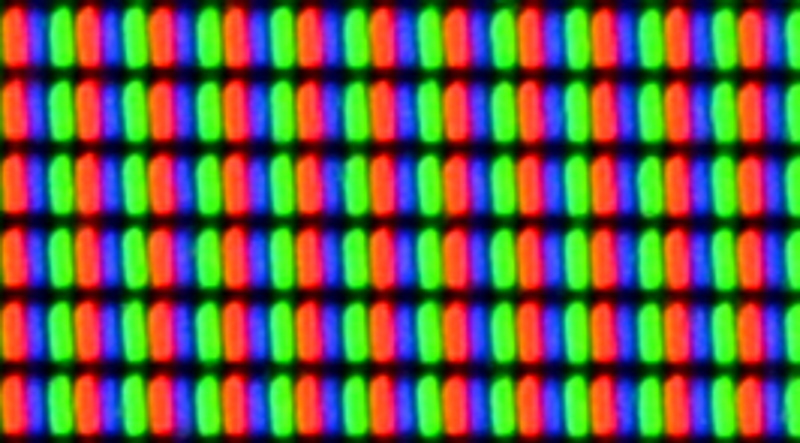
\includegraphics[width=63truemm]{slike/09_LCD.jpg}
\caption{Vsak piksel tekočekristalnega zaslona je sestavljen iz treh barv.}
\end{figure}
\end{remark}

Pokazati moramo še, da polarizacija svetlobe približno sledi zasuku optične osi. 
Vzemimo vzorec, kakršen je na sliki~(\ref{LCD1}\,a) in ga obravnavajmo
kot lokalno optično enoosno snov. Pri $z=0$ naj bo optična
os v smeri $x$, ko se premikamo vzdolž osi $z$, pa naj se optična os suče
v ravnini $xy$. Kot med optično osjo in osjo $x$ tako zapišemo 
\begin{equation}
\varphi=qz.
\label{7.58}
\end{equation}

Poleg zasukane nematične celice je pomemben primer
snovi s takimi lastnostmi holesterični tekoči kristal, ki je zelo
podoben nematičnim, le da je kiralen in se $\mathbf{n}$ spontano suče okoli
smeri, pravokotne na $\mathbf{n}$.
Zanimajmo se le za širjenje svetlobe v smeri $z$. 
Tedaj potrebujemo le del dielektričnega
tenzorja v $xy$ ravnini. 

\begin{definition}
Pokaži, da se dielektrični tenzor v zasukani nematični plasti zapiše kot
\begin{equation}
\varepsilon (z)=\left[\begin{array}{cc}
\bar{\varepsilon}+\frac{1}{2}\varepsilon_{a}\cos(2qz) & \frac{1}{2}\varepsilon_{a}\sin(2qz)\\
\frac{1}{2}\varepsilon_{a}\sin(2qz) & \bar{\varepsilon}-\frac{1}{2}\varepsilon_{a}\cos(2qz)
\end{array}\right],
\label{7.59}
\end{equation}
kjer  je $z$ razdalja od plasti, v kateri je direktor
obrnjen v smeri $x$, povprečna vrednost $\bar{\varepsilon}$ pa  
\begin{equation}
\bar{\varepsilon}=\frac{\varepsilon_{\parallel}+\varepsilon_{\perp}}{2}.
\label{7.60}
\end{equation}
\end{definition}

Iz Maxwellovih enačb~(enačbe~\ref{eq:Maxwell1}--\ref{eq:Maxwell4}) 
hitro uvidimo, da je valovna enačba
za valovanje s frekvenco $\omega$ oblike
\begin{equation}
\frac{d^{2}\mathbf{E}}{dz^{2}}+\frac{\omega^{2}}{c^{2}} \epsilon
(z)\mathbf{E}=0
\label{7.61}
\end{equation}
ali po komponentah, upoštevajoč tenzor dielektričnosti~(enačba~\ref{7.59})
\beq
\frac{d^{2}E_{x}}{dz^{2}} + 
(\beta^{2}+\alpha^{2}\cos(2qz))E_{x}+\alpha^{2}E_{y}\sin(2qz) = 0
\label{7.62a}
\eeq
in 
\beq
\frac{d^{2}E_{y}}{dz^{2}} +
\alpha^{2}E_{x}\sin(2qz)+(\beta^{2}-\alpha^{2}\cos(2qz))E_{y} = 0,
\label{7.62b}
\eeq
kjer je $\alpha^{2}=\epsilon_{a}\omega^{2}/(2c^{2})$ in 
$\beta^{2}=\bar{\epsilon}\omega^{2}/c^{2}$. Dobili smo torej sistem
dveh sklopljenih diferencialnih enačb. 

Za reševanje je ugodno vpeljati krožni polarizaciji 
$E_{+}=E_{x}+iE_{y}$ in $E_{-}=E_{x}-iE_{y}$.
Enačbi~(\ref{7.62a}) in (\ref{7.62b}) prepišemo v
\beq
-\frac{d^{2}E_{+}}{dz^{2}}=\beta^{2}E_{+}+\alpha^{2}E_{-}e^{2iqz}
\label{lcm1}
\eeq
in 
\beq
-\frac{d^{2}E_{-}}{dz^{2}}=\alpha^{2}E_{+}e^{-2iqz}+\beta^{2}E_{-}.
\label{lcm2}
\eeq

Lastne rešitve poiščimo v obliki 
\beq
E_{+}  =  Ae^{i(k+q)z} 
\label{7.65a}
\eeq
in
\beq
E_{-}  =  Be^{i(k-q)z}.
\label{7.65}
\eeq
Nastavek reši sistem enačb~(\ref{lcm1}) in (\ref{lcm2}), 
natanko takrat, kadar $A$ in $B$ rešita sistem homogenih linearnih enačb 
\beq
[(k+q)^{2}-\beta^{2}]A-\alpha^{2}B  =  0 
\eeq
in
\beq
-\alpha^{2}A+[(k-q)^{2}-\beta^{2}]B  =  0.
\eeq
 Sistem je netrivialno rešljiv, če je determinanta koeficientov enaka
nič
\begin{equation}
(k^{2}+q^{2}-\beta^{2})^{2}-4k^{2}q^{2}-\alpha^{4}=0.
\label{7.66}
\end{equation}
Spomnimo se, da sta $\beta$ in $\alpha$ sorazmerna z $\omega$,
zato dobljena enačba predstavlja disperzijsko relacijo -- zvezo med 
$\omega$ in $k$ -- za svetlobo v zavitem sredstvu
\begin{equation}
(k^{2}+q^{2}-\frac{\bar{\epsilon}\omega^{2}}{c^{2}})^{2}-
4k^{2}q^{2}- \frac{\epsilon_{a}^2\omega^{4}}{4c^{4}}
=0.
\label{7.66a}
\end{equation}

V splošnem je iskanje rešitev gornje enačbe zapleten problem, vendar 
za razlago delovanja zasukane nematične celice zadošča približek 
$q\ll\beta$ in $\alpha$, ko je torej perioda sukanja optične osi
velika v primerjavi z valovno dolžino svetlobe. Tedaj lahko $q$ v disperzijski
zvezi (enačba~\ref{7.66}) zanemarimo in dobimo
\begin{equation}
k^{2}=\left\{ \begin{matrix}\beta^{2}+\alpha^{2}=\frac{\omega^{2}}{c^{2}}\epsilon_{\parallel} 
\\               \beta^{2}-\alpha^{2}=\frac{\omega^{2}}{c^{2}}\epsilon_{\bot} 
              \end{matrix}\right.
\label{7.67}
\end{equation}
 Ti vrednosti ustrezata velikosti valovnega vektorja za izredni
in redni val v navadnem enoosnem kristalu. Vstavimo ju v enačbi~(\ref{7.65a}) ali
(\ref{7.65}) in za polarizaciji lastnih valov dobimo $B=\pm A$.

Izračunajmo še obe kartezični komponenti električnega polja za prvo rešitev
\begin{align}
E_{x} &=  \frac{1}{2}(E_{+}+E_{-})  =  \frac{1}{2}Ae^{ikz}(e^{iqz}+e^{-iqz})  =  Ae^{ikz}\cos qz\\
E_{y} & = \frac{1}{2i}(E_{+}-E_{-})  =  \frac{1}{2i}Ae^{ikz}(e^{iqz}-e^{-iqz})  =  Ae^{ikz}\sin qz.
\label{7.68}
\end{align}
Polarizacija torej res sledi optični osi. Druga rešitev da val,
ki je polariziran pravokotno na lokalno optično os in se prav tako
suče z njo. Pri tem se prvi val širi s fazno hitrostjo $c/n_{e}$, torej kot
izredni val, drugi pa s $c/n_{o}$, to je kot redni val. Če na zasukano
nematično celico vpada svetloba, ki je polarizirana ali vzporedno z 
optično osjo ob meji ali pravokotno nanjo, se pojavi na izhodni strani 
polarizacija, zasukana za enak kot, kot je zasukana optična os. 
V primeru, da vpadna polarizacija ne sovpada z eno od
lastnih osi, jo razstavimo na obe lastni in po prehodu skozi
tekoči kristal zopet sestavimo, s čemer seveda v splošnem nastane eliptična
polarizacija.

\begin{remark}
Disperzijsko zvezo (enačba~\ref{7.66} oziroma~\ref{7.66a}) 
lahko rešimo numerično (slika~\ref{gap}). Vidimo, da pri 
vseh frekvencah, razen v ozkem območju -- recimo mu frekvenčna reža --
pri danem $\alpha$ obstajajo štiri realne rešitve za $k$, 
po dve za valovanji v pozitivni in v negativni smeri.
V območju reže je en par rešitev imaginaren. Vsaki vrednosti $k$
pripada neko razmerje amplitud $A$ in $B$, ki ga izračunamo
iz enačb~(\ref{7.65a}) in (\ref{7.65}) in ki določa polarizacijo lastnega vala. Polarizacije
lastnih valov so v splošnem eliptične in pri dani frekvenci med
seboj niso pravokotne, saj zapisani sistem enačb ne predstavlja čisto 
navadnega problema lastnih vektorjev simetrične matrike. 
V območju frekvenčne reže le en par rešitev predstavlja
potujoč val, drug pa polje, ki eksponentno pojema v sredstvo. Zato
se svetloba s frekvenco v reži in z ustrezno polarizacijo, ki vpada
na holesterični tekoči kristal, totalno odbije. Pojav je povsem analogen
Braggovemu odboju na kristalih in daje holesterikom značilen obarvan
videz.\index{Tekoči kristali!Holesterik}
\begin{figure}[h]
\centering
\def\svgwidth{70truemm} 
\input{slike/09_gap.pdf_tex}
\caption{Rešitve disperzijske zveze (enačba~\ref{7.66}) v zasukanem nematiku
pri izbrani $\alpha$. Razen na ozkem frekvenčnem območju obstajajo štiri 
rešitve za vsako frekvenco.}
\label{gap}
\end{figure}
\end{remark}

\section{*Račun preklopa v tekočem kristalu -- Frederiksov prehod}
V prejšnjem razdelku smo omenili, da lahko z dovolj velikim zunanjim poljem 
molekule tekočega kristala, razen tik ob površini, obrnemo v smeri polja. 
Izračunajmo jakost polja, ki je potrebna za ta zasuk. 
\index{Frederiksov prehod}

Energija nematičnega tekočega kristala je najnižja, kadar je direktor $\mathbf{n}$
povsod obrnjen v isto smer. Povečanje energije zaradi krajevne odvisnosti $\mathbf{n}$
v splošnem zapišemo z orientacijsko elastično energijo oziroma Frankovo prosto 
energijo\footnote{Angleški fizik Sir Frederick Charles Frank, 1911--1998.}
\index{Frankova prosta energija}
\boxeq{7.70}{
F_{e}=\frac{1}{2}\int\left\{ K_{1}(\nabla\cdot\mathbf{n})^{2}+K_{2}
[\mathbf{n}\cdot(\nabla\times\mathbf{n})]^{2}+K_{3}
[\mathbf{n}\times(\nabla\times\mathbf{n})]^{2}\right\} dV.
}
Pri tem so $K_{1}$, $K_{2}$ in $K_{3}$ tri Frankove elastične
konstante, ki so odvisne od snovi in tudi od temperature. 
Prvi člen predstavlja povečanje energije zaradi deformacije v obliki 
pahljače, drugi zaradi zasuka, tretji pa zaradi upogiba (slika~\ref{s7.20}).
\begin{figure}[h]
\centering
\def\svgwidth{140truemm} 
\input{slike/09_KKK.pdf_tex}
\caption{Trije načini deformacije ureditve tekočega kristala so pahljačasta deformacija,
zasuk in upogib.}
\label{s7.20}
\end{figure}

V zunanjem električnem polju se energija tekočega kristala dodatno spremeni. 
Navadno je neodvisna električna količina električna poljska jakost, saj je polje posledica
zunanje napetosti na elektrodah. Ustrezni člen v termodinamičnem
potencialu je tedaj (enačbi~\ref{lcwe} in~\ref{7.56a})
\beq
w_{el} = -\frac{1}{2} \mathbf{D}\cdot\mathbf{E} = -\frac{1}{2} 
\left( \varepsilon_0 \varepsilon_\bot \mathbf{E}\cdot\mathbf{E} + 
\varepsilon_{0}\varepsilon_{a}(\mathbf{E}\cdot\mathbf{n})^{2}\right).
\eeq
Prvi člen je neodvisen od $\mathbf{n}$, zato ni pomemben pri izračunu
preklopa. Prosta energija
nematičnega tekočega kristala v električnem polju je tako 
\begin{equation}
F=F_{0}+F_{e}-\frac{1}{2}\varepsilon_{0}\varepsilon_{a}
(\mathbf{E}\cdot \mathbf{n})^{2},
\label{7.72}
\end{equation}
 kjer $F_{0}$ predstavlja del proste energije, ki je neodvisen od $\mathbf{n}$.
Tekoči kristal je v ravnovesju, ko je prosta energija najmanjša. Kadar je
$\epsilon_{a}>0$, se zato skuša $\mathbf{n}$ postaviti vzporedno s
poljem, popoln zasuk pa onemogoča mejna urejevalna plast. 
Da lahko z minimizacijo $F$ izrazimo $\mathbf{n}(\mathbf{r})$, moramo
torej poznati še robne pogoje.

Poglejmo primer. Naj bo nematični tekoči kristal med dvema vzporednima
steklenima ploščama v razmiku $d$. Na obeh ploščah naj bo $\mathbf{n}$ vzporeden
s površino in obrnjen v isto smer, tako da je brez zunanjega 
polja $\mathbf{n}$ povsod enako usmerjen. Naj bo to smer $x$.
Na stekleni plošči dodamo elektrodi, ki ustvarjata polje pravokotno na 
prvotno smer direktorja, naj bo to smer $z$.
Ko priključimo polje, je energijsko ugodnejše, če
se molekule vsaj delno zasučejo v smer polja. Ta zasuk opišemo s
komponento vektorja $\mathbf{n}$ v smeri $z$
\begin{equation}
\mathbf{n}(z)=(n_{x}(z),0,n_{z}(z)).
\label{7.73}
\end{equation}
Robni pogoj, kateremu mora direktor zadostiti,
je $n_{z}(0)=n_{z}(d)=0$. Približno rešitev zato iščemo z nastavkom 
\begin{equation}
n_{z}(z)=a\sin (qz), \qquad q=\frac{\pi}{d},
\label{7.74}
\end{equation}
ki ni nič drugega kot prvi člen razvoja prave rešitve v Fourierevo vrsto.
Ker je direktor enotski vektor, velja
\beq
n_x = \sqrt{1-a^2\sin^2(qz)} \approx 1 - \frac{a^2}{2}\sin^2(qz).
\eeq
Vzdolž smeri $x$ in $y$ se direktor ne spreminja, zato velja
\begin{equation}
\nabla\times\mathbf{n}=(0,\frac{dn_{x}}{dz},0)
\label{7.75}
\end{equation}
 in 
\begin{equation}
\mathbf{n}\times(\nabla\times\mathbf{n})=(-n_{z}\frac{dn_{x}}{dz},0,
n_{x}\frac{dn_{x}}{dz}).
\label{7.76}
\end{equation}
Površinska gostota proste energije je tako 
\begin{eqnarray}
F & = & \frac{1}{2}\int\left[K_{1}\left(\frac{dn_{z}}{dz}\right)^{2}+K_{3}(n_x^2+n_{z}^{2})
\left(\frac{dn_{x}}{dz}\right)^{2}-
\epsilon_{0}\epsilon_{a}(n_{z}E)^{2}\right]dz=\nonumber \\
 & = & \frac{1}{2}\int_{0}^{d}
 [K_{1}q^{2}a^{2}\cos^{2}(qz)+K_{3}q^{2}a^{4}\sin^{2}(qz)\cos^2(qz)-
 \epsilon_{0}\epsilon_{a}E^2a^{2}\sin^{2}(qz)]dz=\nonumber \\
 & = & \frac{\pi}{4q}a^2\left( K_{1}q^{2}+\frac{1}{4}K_{3}q^{2}a^2-\epsilon_{0}\epsilon_{a}E^2\right).
\end{eqnarray}
V našem primeru smo integral lahko izračunali, saj smo uporabili nastavek (enačba~\ref{7.74}).
Sicer bi morali uporabiti Euler-Lagrangeevo metodo za minimizacijo proste energije, ki 
jo poznamo iz variacijskega računa.

Zdaj lahko poiščemo amplitudo deformacije $a$, pri kateri je prosta energija
najmanjša. Tedaj mora biti $a$ rešitev enačbe 
\begin{equation}
2(K_{1}q^{2}-\epsilon_{0}\epsilon_{a}E)a+K_{3}q^{2}a^{3}=0.
\label{7.78}
\end{equation}
 Rešitvi sta 
\begin{equation}
a=0
\end{equation}
in
\beq
a^{2}=2\frac{\epsilon_{0}\epsilon_{a}E^2-K_{1}q^{2}}{K_{3}q^{2}}.
\label{7.79}
\eeq
 Pri majhnih poljih, ko je $\epsilon_{0}\epsilon_{a}E^2<K_{1}q^{2}$,
je fizikalno smiselna le prva rešitev, torej brez deformacije, pri velikih poljih pa je  
stabilna druga rešitev. Ko večamo polje, deformacija
v sredini plasti hitro naraste, tako da se $\mathbf{n}$ postavi skoraj
popolnoma v smer zunanjega polja. Tedaj naša rešitev seveda ni dobra,
saj smo pri računu privzeli, da je $n_{z}\ll1$. Prehodu iz nedeformiranega
stanja v deformirano stanje pravimo tudi Frederiksov prehod\footnote{Ruski fizik
Vsevolod Konstantinovič Frederiks, tudi Fr\'{e}edericksz, 1885--1944.}. Na njem
temelji preklapljanje optičnih prikazovalnikov na nematične tekoče kristale.

Izračunajmo še kritično jakost električnega polja, pri kateri pride do prehoda v deformirano fazo.
To se zgodi pri 
\beq
\epsilon_{0}\epsilon_{a}E_c^2-K_{1}q^{2} = 0
\eeq
oziroma
\boxeq{FreeE}{
E_c = \frac{\pi}{d}\sqrt{\frac{K_1}{\varepsilon_0\varepsilon_a}}.
}

Poglejmo še, kako narašča amplituda deformacije v bližini prehoda. Iz enačbe~(\ref{7.79})
sledi 
\beq
a = \sqrt{\frac{2 \varepsilon_0 \varepsilon_a}{K_3 q^2 }(E^2-E_c^2)}.
\eeq
Pogosto naredimo približek enakih konstant, kjer privzamemo, da so vse Frankove 
elastične konstante enake vrednosti. V tem približku je 
\beq
a \approx \sqrt{\frac{2(E^2-E_c^2)}{E_c^2}}
\eeq
in torej korensko narašča s naraščajočim poljem (slika~\ref{Fred}). Tak prehod je torej
fazni prehod drugega reda, saj količina, ki opisuje prehod (amplituda deformacije $a$)
zvezno preide iz vrednosti $a=0$ v končno vrednost. 
\begin{figure}[h]
\centering
\def\svgwidth{80truemm} 
\input{slike/09_Fred.pdf_tex}
\caption{Kvalitativno obnašanje amplitude deformacije ob Frederiksovem prehodu}
\label{Fred}
\end{figure}

\begin{definition}
Izračunaj Frederiksov prehod v zasukani nematični celici (kot zasuka med zgornjo in spodnjo 
mejno ploskvijo naj bo $\pi/2$) in pokaži, da je kritično polje za prehod enako
\beq
E_c =  \frac{\pi}{d}\sqrt{\frac{K_1}{\varepsilon_0\varepsilon_a}}
\sqrt{1 + \frac{K_3-2K_2}{4K_1}}.
\eeq
Namig: uporabi nastavek $\varphi = z \pi/2d$ in $\vartheta = a \sin(\pi z/d)$. 
\end{definition}


%Končano
%-------------------------------------------------------------------------------
%	CHAPTER 10
%-------------------------------------------------------------------------------

\chapterimage{Mavrica.jpg} % Chapter heading image

\chapter{Optična vlakna}
Moderna komunikacijska tehnologija zahteva vedno hitrejši prenos
vedno večje količine informacij. Navadne kovinske vodnike
so zato v računalniških in telefonskih povezavah nadomestila optična 
vlakna, ki jih odlikujejo majhne izgube, neobčutljivost na elektromagnetne
in medsebojne motnje ter zmožnost prenosa izjemno velike količine podatkov. 

\section{Planparalelni vodnik}
\subsection{Klasična razlaga}
Klasično lahko razložimo delovanje optičnih vlaken s totalnim odbojem
na meji med dvema plastema. Kadar prehaja svetloba iz snovi 
z večjim lomnim količnikom v sredstvo z manjšim lomnim količnikom,
se pri kotih, ki so večji od kritičnega kota, totalno odbije. 
\begin{figure}[h]
\centering
\def\svgwidth{120truemm} 
\input{slike/10_Vodnik.pdf_tex}
\caption{Klasična razlaga valovnega vodnika}
\label{fig:vodnik}
\end{figure}

Najpreprostejši model optičnega vodnika je planparalelna plast prozornega
dielektrika z lomnim količnikom $n_{1}$, ki je večji od lomnega količnika
okolice $n_2$ (slika~\ref{fig:vodnik}). 
Plasti z večjim lomnim količnikom rečemo sredica, okolici
pa plašč vodnika. Žarek je ujet v sredici, če je vpadni kot 
na mejno plast $\vartheta$ večji od kota totalnega odboja, 
za katerega velja 
\boxeq{10totalni}{
\sin\vartheta_{c}=\frac{n_{2}}{n_{1}}.
}
Količini, ki določa največji kot divergence svetlobnega snopa, 
ki vpada na vodnik in ostane v njem ujet, pravimo
numerična odprtina vlakna. Izračunamo jo kot 
\beq
NA = \sin \alpha = n_1 \sin \beta = 
n_1 \sin(\pi/2-\vartheta_c) =
n_1 \cos\vartheta_c = n_1 \sqrt{1-\sin^2\vartheta_c}.
\eeq
Upoštevajoč enačbo~(\ref{10totalni}) sledi 
\boxeq{10NA}{
NA = \sqrt{n_1^2-n_2^2}.
}
Ker je razlika lomnih količnikov v vodnikih razmeroma majhna,
tipično le nekaj stotink, je tudi numerična apertura optičnih 
vodnikov navadno
$NA \lesssim 0,1 $. Kot, pod katerim lahko vpada svetloba
v vlakno, da se v njega ujame, je zato zelo majhen. 

\subsection{Valovni opis}
Za podroben opis širjenja svetlobe po vodnikih ali vlaknih, 
ki imajo navadno polmer
sredice od nekaj do nekaj deset mikrometrov, geometrijska optika ne
zadošča. Rešiti moramo Maxwellove enačbe (enačbe~\ref{eq:Maxwell1}--\ref{eq:Maxwell4}) 
z ustreznimi robnimi pogoji (enačbe~\ref{eq:robni-pogoji}--\ref{eq:robni-pogoji5}),
kar je za praktična vlakna dokaj dolg račun. Zato ugotovimo najprej, kakšne
so osnovne značilnosti valovanja, ki se širi po vodniku.

Glede na smer polarizacije električne poljske jakosti 
ločimo dva različna primera. Če leži električna poljska
jakost vzporedno z mejnima ploskvama (smer $y$), 
govorimo o transverzalnem električnem (TE) valovanju. 
V nasprotnem primeru, ko je 
z mejnima ploskvama vzporedna magnetna poljska jakost in 
leži električna poljska jakost v ravnini $xz$, 
govorimo o transverzalnem magnetnem (TM) valovanju.
\begin{figure}[h]
\centering
\def\svgwidth{120truemm} 
\input{slike/10_TETM.pdf_tex}
\caption{TE in TM polarizaciji v valovnem vodniku}
\label{fig:TETM}
\end{figure}

Geometrijskemu žarku, ki pod kotom potuje po sredici in se na njeni meji
odbija, ustreza v valovni sliki val, ki ima prečno komponento valovnega
vektorja $k_{x}$ različno od nič. Ker je valovanje v prečni smeri 
omejeno na sredico končne dimenzije (naj bo to debelina plasti $a$), ima lahko
$k_{x}$ le diskretne vrendosti, ki so približno enake $N\pi/a$. Pri 
tem je $N$ celo število in je enako številu vozlov, ki jih ima valovanje v prečni smeri.
Pravimo tudi, da vsak $N$ določa en rod valovanj v vlaknu. Po drugi strani 
pa obstaja v vodniku največji $k_x$, ki je določen 
s kotom totalnega odboja 
\beq
k_{x \mathrm{max}} \approx k_0 n_1 \cos\vartheta_c = k_0 \sqrt{n_1^2 -n_2^2}.
\eeq
Številom možnih rešitev za $k_x$ je torej omejeno in točno določeno, odvisno
pa je od razlike lomnih količnikov in od dimenzije vodnika oziroma vlakna. 
V nadaljevanju bomo spoznali, da v optičnih vlaknih en rod vselej obstaja,
za razliko od dielektričnih in kovinskih vodnikov, kakršne
poznamo iz mikrovalovne tehnike, po katerih se pod določeno frekvenco
valovanje ne more širiti. Optični vodniki, po katerih se širi
en sam rod, imajo posebej lepe lastnosti za uporabo v komunikacijskih
sistemih.

Povejmo še nekaj o hitrosti valovanja v vlaknu.
Naj bo $\beta$ komponenta valovnega vektorja vzdolž
vlakna, recimo ji tudi valovno število, tako da je odvisnost polja
od koordinate vzdolž vlakna $\exp (i\beta z)$. Po drugi strani pa velja
zveza
\begin{equation}
n_{1}\frac{\omega}{c_0}=\sqrt{\beta^{2}+k_{x}^{2}}
\label{9.0}.
\end{equation}
Za dano vrednost $k_{x}$ torej zveza med valovnim številom $\beta$
in frekvenco $\omega$ ni linearna, zato je fazna hitrost $v_{f}=\omega/\beta$
odvisna od frekvence in pride do disperzije. Grupna hitrost $v_{g}=d\omega/d\beta$ 
je zaradi nelinearne odvisnosti različna od fazne hitrosti in tudi odvisna od 
frekvence, kar ima za uporabo vlaken pomembne posledice. Več o tem bomo spoznali 
proti koncu poglavja. 

\section{Račun lastnih rodov v planparalelnem vodniku}
Poiščimo zdaj rešitve valovne enačbe v planparalelnem vodniku. 
To je preprost dvodimenzionalen model optičnega vlakna, ki je sestavljen iz 
plasti prozornega dielektrika in plašča, ki naj bo zaradi enostavnosti na obeh 
straneh sredice enak. 
\begin{figure}[h]
\centering
\def\svgwidth{120truemm} 
\input{slike/10_VodnikRacun.pdf_tex}
\caption{K izračunu lastnih rodov v vodniku}
\label{fig:vodnikracun}
\end{figure}

Krajevni del valovne enačbe, ki jo rešujemo,
je
\beq
\nabla^{2}\mathbf{E}+n\left(x\right)^{2}k_{0}^{2}\mathbf{E}=0,
\label{9.1}
\eeq
kjer je $k_{0}=\omega/c$, $n$ pa nezvezno spremeni vrednost, ko preidemo iz sredice v plašč. 
Rešitev iščemo v obliki 
\begin{equation}
{\mathbf E}(x,z)=\mathbf{e}\psi\left(x\right)\, e^{i\beta z}.
\label{9.2}
\end{equation}
Omejimo se le na primer TE polarizacije (za izračun lastnih rodov TM polariziranega
valovanja glej nalogo~\ref{naloga:TM}). Vstavimo nastavek (enačba~\ref{9.2}) v valovno enačbo
(\ref{9.1}) in dobimo
\begin{equation}
\frac{d^{2}{\bf \psi}}{dx^{2}}+\left(k_{0}^{2}n_1^{2}-\beta^{2}\right){\bf \psi}=0
\qquad \textrm{v sredici oziroma obmo\v cju II} 
\label{9.3}
\end{equation}
in 
\begin{equation}
\frac{d^{2}{\bf \psi}}{dx^{2}}+\left(k_{0}^{2}n_2^{2}-\beta^{2}\right){\bf \psi}=0
\qquad \textrm{v plašču oziroma obmo\v cjih I in III.} 
\label{9.3}
\end{equation}
Ker je po enačbi~(\ref{9.0}) $k_0^2n_1^2-\beta^2=k_x^2$, lahko rešitve prve enačbe
zapišemo v obliki
\beq
\psi_{\mathrm{II}}(x) = C \cos(k_x x)+D \sin(k_x x).
\eeq
Rešitve v plašču pa so oblike
\beq
\psi_{\mathrm{I}}(x) = A \exp(-\kappa x)+B \exp(\kappa x),\\
\psi_{\mathrm{III}}(x) = E \exp(-\kappa x)+F \exp(\kappa x),
\eeq
pri čemer je $\kappa^2= \beta^2-n_2^2k_0^2$.

Če želimo, da je valovanje ujeto v vlakno, mora biti $\kappa$ realno število.
Le tako namreč dosežemo eksponentno pojemanje z oddaljenostjo od sredice,
sicer je valovanje v vseh treh območjih oscilatorno in ni ujeto v vlakno. 
Tako dobimo pogoj za valovno število $\beta$
\boxeq{vlaknobeta}{
k_0n_2 < \beta < k_0 n_1.
}

Zahteva po končnost rešitve da pogoj, da je v območju I (pri $x>a/2$) $B=0$, 
v območju III (pri $x<-a/2$) pa $E=0$. Dodatne omejitve se pojavijo zaradi 
simetrije problema, saj so rešitve lahko le sode ali lihe funkcije. Tako 
dobimo dve vrsti rešitev, sode in lihe:
\begin{align}
\psi_{\mathrm{I}}(x) =&~ A \exp(-\kappa x), \qquad \qquad &\psi_{\mathrm{I}}(x) =&~ A \exp(-\kappa x),\\
\psi_{\mathrm{II}}(x) =&~ C \cos(k_x x), \qquad \qquad &\psi_{\mathrm{II}}(x) =&~ D \sin(k_x x)\\
\psi_{\mathrm{III}}(x) =&~ A \exp(\kappa x), \qquad \qquad &\psi_{\mathrm{III}}(x) =&~ -A \exp(\kappa x).
\end{align}
Zvezo med koeficienti določimo z upoštevanjem robnih pogojev. Na meji
med sredico in plaščem morata biti tangencialni komponenti 
električne in magnetne poljske jakosti zvezni. Iz tega takoj 
izluščimo pogoj, da se za TE valovanje na meji ohranja amplituda električne poljske jakosti.
Drugi pogoj dobimo iz zveze $\nabla\times{\bf E}=i\omega\mu_{0}{\bf H}$, ki izhaja
neposredno iz Maxwellove enačbe~(\ref{eq:Maxwell2}). Ta pogoj zahteva, da se na meji ohranja
odvod električne poljske jakosti $dE/dx$. Tako pogoje za sode in lihe rešitve zapišemo kot
\beq
A \exp(-\kappa a/2) = C \cos(k_x a/2), \qquad \qquad A \exp(-\kappa a/2) = D \sin(k_x a/2).
\eeq
in 
\beq
-A \kappa \exp(-\kappa a/2) = -C k_x \sin(k_x a/2), \qquad
-\kappa A \exp(-\kappa a/2) = D k_x \cos(k_x a/2).
\eeq
Enačbo, ki določa rešitev $k_x$, dobimo iz zahteve, da sta gornja robna pogoja hkrati izpoljnjena. Za sode 
načine tako velja
\boxeq{sekular1}{
\frac{\kappa}{k_x} = \tan \frac{k_x a}{2},
}
za lihe pa 
\boxeq{sekular2}{
-\frac{k_x}{\kappa} = \tan \frac{k_x a}{2}.
}
Pri tem zapišimo še zvezo med $k_x$ in $\kappa$
\boxeq{kappak}{
k_x^{2}+\kappa^{2}=k_{0}^{2}\left(n_{1}^{2}-n_{0}^{2}\right).
}
Sekularnih enačb za lastne načine nihanj ne moremo rešiti analitično. Zato jih rešujemo numerično,
zelo nazorna pa je grafična predstavitev. S slike~(\ref{fig:TEsec}) lahko namreč hitro razberemo
število rešitev in njihove vrednosti. Najprej narišemo desno stran enačb~(\ref{sekular1}) 
in~(\ref{sekular2}), to je $\tan (k_x a/2)$ (črna črta). 
Nato narišemo še levi strani enačb, pri čemer upoštevamo zvezo~(\ref{kappak}), rdeča krivulja naj 
bo za sode rešitve in modra za lihe rešitve. Število presečišč rdeče in modre krivulje s črno
 da število rodov, ki se lahko razširjajo po takem vlaknu. V našem primeru je takih rodov pet:
 trije sodi in dva liha. Z grafa razberemo  še eno pomembno lastnost. Ne glede na to, kako tanek
 je vodnik, vedno bo obstajala vsaj ena rešitev za $k_x$, saj rdeča krivulja vedno nekje seka črno. 
 Vlaknu, v katerem se širi samo eno valovanje, pravimo enorodnovno vlakno, sicer so vlakna večrodovna.
 Za tipično enorodovno vlakno velja $a\lesssim 5~\mu$m, za večrodovno z okoli 20 rodovi pa 
 $a\sim 50~\mu$m.
\begin{figure}[h]
\centering
\def\svgwidth{90truemm} 
\input{slike/10_TEsekularna.pdf_tex}
\caption{K izračunu prečnih komponent valovnega vektorja v planparalelnem valovnem vodniku
za TE polarizacijo. V skiciranem primeru je vodnik petrodoven.}
\label{fig:TEsec}
\end{figure}

Ocenimo število možnih rodov še z izračunom. S slike~(\ref{fig:TEsec}) vidimo, da je največja možna 
vrednost valovnega vektorja $k_x$, pri kateri valovanje še potuje po vlaknu, omejena z vrednostjo, 
pri kateri $\kappa$ pade na nič. Do te vrednosti pa je po ena rešitev na vsakih $\pi/a$. Celotno 
število rodov je tako
\beq
N \approx \frac{k_{x\mathrm{max}}}{\pi/a}  = \frac{k_0 a NA }{\pi},
\eeq
pri čemer smo uporabili zvezo~(\ref{kappak}) ob pogoju, da je $\kappa =0$. 

Ko enkrat izračunamo dovoljene vrednosti $k_x$, končno poznamo celotno električno poljsko
jakost v vodniku in izven njega. Za primer s slike~(\ref{fig:TEsec}) so osnovni načini 
narisani na sliki~(\ref{fig:TESodi}).
\begin{figure}[h]
\centering
\def\svgwidth{70truemm} 
\input{slike/10_TESodi.pdf_tex} 
\quad
\def\svgwidth{70truemm} 
\input{slike/10_TELihi.pdf_tex} 
\caption{Osnovni načini za širjenje svetlobe po valovnem vodniku, levo so sode rešitve, desno pa lihe.}
\label{fig:TESodi}
\end{figure}

Osnovna lastna vrednost $\xi_{0}$ je pri $V<<1$ približno kar $V$.
Zato je $k_{\perp}^{2}\simeq k_{0}^{2}(n_{1}^{2}-n_{0}^{2})$ in je
$\beta=n_{0}k_{0}$. V primeru zelo šibkega vodenja je torej fazna
hitrost vodenega vala približno enaka fazni hitrosti v plašču, to
je $c/n_{0}$. To je lahko razumeti; pri majhnem $V$ je namreč tudi
$\kappa$ majhen in se eksponentno pojemajoče valovanje razteza daleč
v plašč. (Naloga:Kakšna je v tej limiti grupna hitrost?). V nasprotnem
primeru, ko je $V>>1$, je $\xi_{0}\simeq\pi/2<<V$. Zato je tudi
$k_{\perp}\simeq\pi/(2a)$ $<<n_{1}k_{0}$ in je približno $\beta\simeq n_{1}k_{0}$.
V tem primeru je torej fazna hitrost taka kot v sredstvu z lomnim
količnikom sredice, kar je v skladu s preprosto predstavo, da se pri
velikem $V$ osnovni vodeni rod širi po sredici vzdolž osi vlakna.

Račun za transverzalno magnetne (TM) valove je zelo podoben, le v
robnem pogoju za tangencialno komponento električnega polja nastopita
dielektrični konstanti sredice in plašča, zato je predvsem najnižja
lastna vrednost za $k_{\perp}$ nekoliko večja kot za TE valove. (Naloga)

\begin{definition}
\label{naloga:TM}
Ponovi izračun za TM valovanje in pokaži, da se sekularni enačbi v primeru TM polarizacije
zapišeta kot 
\beq
\frac{\kappa}{k_x} = \tan \frac{k_x a}{2} \qquad \mathrm{in} \qquad -\frac{k_x}{\kappa} = \tan \frac{k_x a}{2}.
\eeq
\end{definition}


za delec v končno globoki enodimenzionalni potencialni jami v kvantni
mehaniki, kjer lastni vrednosti energije ustreza $\beta^{2}$. 

\section{Cilindrično vlakno}

Običajna vlakna so seveda tridimenzionalna s cilindrično geometrijo.
Najpreprostejša strukutra, povsem analogna gornjemu primeru planparalene
plasti, je jedro s konstatnim lomnim količnikom, ki je nekoliko večji
od lomnega količnika plašča. Pogoste so tudi zapletenejše konstrukcije,
pri katerih je sredica sestavljena iz več kolobarjev z različnimi
lomnimi količniki. S primerno izbiro je tako mogoče zelo zmanjšati
disperzijo (Slika \ref{sl9.3}).

Račun za širjenje svetlobe po cilindričnem vlaknu s homogeno sredico
je sicer podoben kot za planparalelni primer, vendar je precej bolj
zapleten. Glavna komplikacija je, da v cilindrični geomteriji ni več
delitve na čisto električno in magnento transverzalne valove, zato
postanejo robni pogoji bolj zapleteni. Rešitve se izrazajo v obliki
kombinacij Besselovih funkcij. Podrobnosti si bralec lahko ogleda
v literaturi. Osnovne značilnosti rešite pa ostajajo
enako kot v dvodimenzionalnem primeru. Kot smo ugotovili že na začetku,
obstaja končno število vodenih valov, odvisno od premera sredice in
razlike lomnih količnikov sredice in plašča. Če sta ti količini majhni,
obstaja le eno vodeno valovanje in imamo enorodovno vlakno. Za njegovo
valovno število velja $n_{0}k_{0}<\beta<n_{1}k_{0}$.


\section{Cilindrično vlakno s paraboličnim profilom lomnega količnika}

V treh dimenzijah lahko hitro poiščemo rešitve za vlakno, v katerem
je dielektrična konstanta kvadratna funkcija radialne koordinate $r$:
\begin{equation}
n\left(r\right)^{2}=n_{0}^{2}+n_{2}^{2}\, r^{2}\label{9.15}
\end{equation}
 Parameter $n_{2}$ je v praksi vselej majhen, zato ima za vse smiselne
vrednosti $r$ tudi lomni količnik paraboličen profil. Parabolična
sredica mora sveda biti omejena, okoli nje imamo zopet plašč s konstantnim
lomnim količnikom (Slika \ref{sl9.4}). Tipičen radij sredice je nekaj
deset mikrometrov.

Komponento polja za izbrano polarizacijo napišimo v obliki 
\begin{equation}
E=E_{0}\psi(x,y)\, e^{i\beta z}\label{9.16}
\end{equation}
 Zanemarili smo, da zaradi odvisnosti od prečnih koordinat in $\nabla\cdot{\bf E}=0$
polje ne more imeti povsod iste smeri; če hočemo biti natančni, moramo
v gornji obliki zapisati vektorski potencial. Postavimo približni
nastavek v valovno enačbo. Dobimo enačbo 
\begin{equation}
\nabla_{\perp}^{2}\psi+\left[k_{0}^{2}\left(n_{0}^{2}+n_{2}^{2}r^{2}\right)-\beta^{2}\right]\,\psi=0\label{9.17}
\end{equation}
 ki je popolnoma enaka enačbi za krajevni del lastnih funkcij dvodimenzionalnega
harmonskega oscilatorja v kvantni mehaniki. Rešitve imajo obliko 
\begin{equation}
\psi_{lm}=H_{l}\left(\sqrt{2}\frac{x}{w}\right)\, H_{m}\left(\sqrt{2}\frac{y}{w}\right)\, e^{-(x^{2}+y^{2})/w^{2}},\qquad w^{2}=\frac{\lambda}{\pi n_{2}}\label{9.18}
\end{equation}
 z lastnimi vrednostmi 
\begin{equation}
\beta_{lm}^{2}=n_{0}^{2}k_{0}^{2}\left[1-\frac{2n_{2}}{k_{0}n_{0}}\left(l+m+1\right)\right]\label{9.19}
\end{equation}
 Razmerje $2n_{2}/\left(k_{0}n_{0}\right)$ je majhno, zato je približno
$\beta_{lm}=n_{0}k_{0}\left[1-\frac{n_{2}}{k_{0}n_{0}}\left(l+m+1\right)\right].$Če
je $n_{2}$ neodvisen od frekvence, je grupna hitrost 
\begin{equation}
v_{g}=\left(\frac{d\beta_{lm}}{d\omega}\right)^{-1}=\frac{c_{0}}{n_{0}}\label{9.21}
\end{equation}
 enaka za vse rodove, kar je značilnost vlakna s kvadratnim profilom
lomnega količnika. V dejanskem vlaknu je seveda taka odvisnost možna
le v omejenem območju sredice, zato je tudi gornja analiza le približna
in velja dobro za tiste rodove, ki se ne raztezajo izven sredice.

Neodvisnost grupne hitrosti od reda valovanja v vlaknu je praktično
pomembna. Grupna hitrost določa čas potovanja svetlobnega sunka, ki
lahko predstavlja en bit informacije. Če se po vlaknu lahko širi več
rodov, ki imajo različno grupno hitrost, se sunek po prehodu skozi
vlakno razširi, kar omejuje uporabno dolžino vlakna, kot bomo podrobneje
videli kasneje. Temu se lahko izognemo z uporabo enorodovnih vlaken,
ki pa so dražja in je vanje te\textquotedbl{}je uvesti svetlobni snop,
katerega divergenca in premer morata ustrezati ujetemu valu enorodovnega
vlakna, če naj ne bo izgub. Zato se za krajše zveze uporabljajo mnogorodovna
vlakna, ki imajo sredico s približno paraboličnim profilom lomnega
količnika.


\section{Sprememba lomnega količnika vlakna}

Sprememba lomnega količnika sredice ali plašča vlakna povzroči spremembo
valovnega števila $\beta$ danega roda. V enorodovnih vlaknih je to
mogoče izkoristiti za izdelavo senzorjev, na primer temperature ali
tlaka. Zaradi zunanjih vplivov, ki jih želimo zaznati, se spremeni
lomni količnik vlakna in s tem propagacijska konstanta, kar lahko
izmerimo preko spremembe faze valovanja na izhodu iz vlakna, to je,
z ustrezno sestavljenim interferometrom. Ker je dolžina vlakna lahko
velika, v nekaj centimetrov velik tulec lahko brez težav navijemo
kilometre vlakna, je celotna sprememba faze velika že pri majhnih
spremembah merjene količine. Sprememba valovnega števila povzroča
tudi nezaželjene spremembe faze in odboje pri prenosu informacij.
V tem razdelku zato poglejmo, kako se spremeni valovno število pri
dani spremembi lomenga količnika.

Vzemimo rod vlakna s propagacijsko konstanto $\beta_{lm}$ in prečnim
profilom $\psi_{lm}\left(r,\phi\right).$ Ta mora zadoščati valovni
enačbi 
\begin{equation}
\nabla_{\bot}^{2}\psi_{lm}+\left(\epsilon(r)k_{0}^{2}-\beta_{lm}^{2}\right)\psi_{lm}=0\label{9.22}
\end{equation}
 Naj se dielektrična konstanta vlakna spremeni za $\delta\epsilon.$
Zato se spremenita tudi propagacijska konstanta $\beta=\beta_{lm}+\delta\beta$
in prečna oblika $\psi=\psi_{lm}+\delta\psi.$ Tudi motena funckija
$\psi$ mora zadoščati enačbi \ref{9.22}, zato za perturbacijo velja
\begin{equation}
\nabla_{\bot}^{2}\delta\psi+\left(\epsilon(r)k_{0}^{2}-\beta_{lm}^{2}\right)\delta\psi+\delta\epsilon\, k_{0}^{2}\psi_{lm}=2\beta_{lm}\delta\beta\,\psi_{lm}\label{9.23}
\end{equation}
 kjer smo zanemarili produkte majhnih količin. Množimo obe strani
enačbe s $\psi_{lm}^{*}$ in integrirajmo po preseku vlakna, pri čemer
upoštevajmo, da je $\delta\psi$ ortogonalna na $\psi_{lm}$: 
\begin{eqnarray}
 &  & \int\psi_{lm}^{*}\nabla_{\bot}^{2}\delta\psi\, dS+\int\left(\epsilon(r)k_{0}^{2}-\beta_{lm}^{2}\right)\delta\psi\,\psi_{lm}^{*}+k_{0}^{2}\int\delta\epsilon\,\left|\psi_{lm}\right|^{2}dS\label{9.24}\\
 & = & 2\beta_{lm}\,\delta\beta\int\left|\psi_{lm}\right|^{2}dS
\end{eqnarray}
 Prvi člen na levi preoblikujmo z uporabo zvez $\int(u\,\nabla_{\bot}^{2}v-v\nabla_{\bot}^{2}u)\, dS=\int\nabla_{\bot}\cdot(u\nabla_{\bot}v-v\nabla_{\bot}u)\, dS=\oint{\bf ds\times(}u\,\nabla_{\bot}v-v\,\nabla_{\bot}u)$.
Ker fuknciji $\psi_{lm}$ in $\delta\psi$ opisujeta vodene valove,
morata iti za velike $r$ proti nič, zato je integral po krivulji
v gornji zvezi nič in velja $\int\psi_{lm}^{*}\nabla_{\bot}^{2}\delta\psi\, dS=\int\delta\psi\nabla_{\bot}^{2}\psi_{lm}^{*}\, dS$.
Ker $\psi_{lm}^{*}$ zadošča enačbi \ref{9.22}, se v enačbi \ref{9.24}
prvi in drugi člen uničita in dobimo željeno zvezo 
\begin{equation}
\delta\beta=\frac{k_{0}^{2}\int\delta\epsilon\,\left|\psi_{lm}\right|^{2}dS}{2\,\beta\int\left|\psi_{lm}\right|^{2}dS}\label{9.25}
\end{equation}
 ki je seveda analogna kvantnomehanskemu rezultatu s teorijo motenj
prvega reda za spremembo energije lastnega stanja pri majhni sprmembi
Hamiltonovega operatorja. Rezultat je tudi intuitivno razumljiv: v
najnižjem redu je $\delta\beta$ sorazmerna s uteženim povprečjem
$\delta\epsilon$, kjer je utež $\psi_{lm}$.

Sprememba valovnega števila $\beta$ v delu vlakna, po katerem potuje
svetloba, ne povzroči le spremembe faze, ampak tudi odboj dela valovanja.
Ta pojav je le nekoliko druga oblika odboja na meji (zvezni ali ostri)
dveh dielektrikov, ali splošneje, odboja vsakega valovanja na območju,
kjer se spremeni fazna hitrost valovanja.

Odboj na območju vlakna, kjer se spreminja $\beta$, bomo najlažje
dobili preko formule za odboj na meji dveh dielektrikov pri pravokotnem
vpadu. Odbita amplituda je tedaj 
\begin{equation}
E_{r}=\frac{n_{2}-n_{1}}{n_{2}+n_{1}}E_{0}\label{9.26}
\end{equation}
 Mislimo si, da je sprememba $\beta$ na delu vlakna sestavljena iz
majhnih stopničastih sprememb $\Delta\beta_{i}$ na intervalih $\Delta\dot{z}$.
Za ravno valovanje, za katerega velja enačba \ref{9.26}, je sprememba
lomnega količnika sorazmerna s spremembo fazne hitrosti. Ker tudi
$\beta$ določa fazno hitrost valovanja po vlaknu, je delež odbitega
valovanja na stopničasti spremembi $\Delta\beta_{i}$
\begin{equation}
\Delta E_{i}=\frac{\Delta\beta_{i}}{2\,\beta}\, E_{0}\label{9.27}
\end{equation}
 Predpostavili smo, da je celotni del odbitega valovanja tako majhen,
da ni treba upoštevati spremembe amplitude vpadnega vala $E_{0}$.
Vse odbito valovanje je vsota prispevkov na posameznih stopnicah $\Delta\beta_{i}$,
pri čemer moramo upoštevati še različne faze delnih odbitih valovanj:
\begin{equation}
E_{r}=\sum\frac{\Delta\beta_{i}}{2\,\beta}\, e^{2i\beta z_{i}}\, E_{0}=\frac{1}{2\,\beta}\sum\frac{d\beta}{dz}\, e^{2i\beta z_{i}}\Delta z\, E_{0}\label{9.28}
\end{equation}
 Preidimo z vsote na integral, pa dobimo, da je odbita amplituda 
\begin{equation}
E_{r}=\frac{E_{0}}{2\,\beta}\,\int\frac{d\beta}{dz}\, e^{2i\beta z}dz\label{9.29}
\end{equation}


\textit{Primer:} Naj se valovno število linearno spermeni za $\Delta\beta_{0}$
na razdalji $L$. Tedaj je po gornji formuli 
\begin{equation}
\frac{E_{r}}{E_{0}}=2\,\frac{\Delta\beta_{0}}{L}\,\frac{\sin\beta L/2}{\beta}\label{9.30}
\end{equation}
 Odbojnost je največja, kadar je $L$ majhen v primeri z $1/\beta$,
torej kadar je sprememba $\beta$ ostra stopnica. Čim počasnejša je
sprememba, tem manj je odboja, poleg tega pa odboja ni vsakič, ko
je $\sin\beta L/2=0$, to je, pride do destruktivne interference vseh
delnih odbojev.(Naloga: Odboj na erf stopnici).


\section{Izgube v optičnih vlaknih}

Ena najpomembnejših lastnosti optičnih valken je majhno slabljenje
svetlobnega vala, posebej še v vlaknih iz kremenovega stekla. Najboljša
vlakna imajo danes izgube okoli 0,2 db/km pri valovni dolžini 1,55
$\mu$m. (1 decibel je$\,0,1\,$log$(j_{0}/j).$). Glavni vzroki izgub
so absorpcija in sipanje na nečistočah in sipanje na termičnih fluktuacijah
gostote (Rayleighovo sipanje). Slika \ref{sl9.5} prikazuje tipično
odvisnost izgub od valovne dolžine za dobro enorodovno vlakno iz kremenovega
stekla s primesjo GeO$_{2}.$ Sipanje na fluktuacijah gostote je sorazmerno
z $\lambda^{-4}$, zato dominira pri majhnih valovnih dolžinah, sipanje
na defektih in nepravilnostih je skoraj zanemarljivo, pri valovnih
dolžinah nad 1,6~$\mu$m pa prevlada absorpcija. Vrh med 1,3~$\mu$m
in 1,5~$\mu$m je posledica absorpcije na OH ionih, ki se jih je
v steklu zelo težko znebiti. Iz slike je razvidno, da so izgube najmanjše
okoli 1,55~$\mu$m, zato se to območje največ uporablja za zveze
na velike razdalje. Najboljših modernih vlaken tudi ni več mogoče
kaj dosti izboljšati glede izgub, saj so že dosegla spodnjo mejo,
določeno s termičnimi fluktuacijami.

Pri optičnih zvezah nastanejo še izgube na spojih vlaken, ki so okoli
0,2 db na spoj. Skupne izgube so tako dosti manjše kot v koaksialnem
kablu in je možen prenos signala do nekaj sto kilometrov brez vmesnega
ojačevanja. S tem pri dolžini optičnih zvez izgube niso več glavna
omejitev, ampak je to popačitev signala zaradi disperzije.

V optičnem vlaknu nastanejo izgube tudi, kadar je vlakno ukrivljeno.
Te izgube postanejo znantne, kadar je krivinski radij vlakna centimeter
ali manj. Ta pojav je dovolj zanimiv, da si ga je vredno nekoliko
podrobneje ogledati.

Vzemimo spet dvodimenzionalno plast debeline $2a$ z lomnim količnikom
$n_{1}$ v sredstvu z lomnim količnikom $n_{0},$ ki naj bo ukrivljena
s krivinskim radijem $R$. Taka plast tvori del kolobarja z notranjim
radijem $R-a$ in zunanjim radijem $R+a$, pri čemer je $\dot{R}>>a$
(Slika \ref{sl9.6}). Zapišimo valovno enačbo za dve dimenziji v cilindrični
geometriji: 
\begin{equation}
\frac{1}{r}\,\frac{\partial}{\partial r}\, r\,\frac{\partial E}{\partial r}+\frac{1}{r^{2}}\,\frac{\partial^{2}E}{\partial\phi^{2}}+k_{0}^{2}n^{2}\left(r\right)\, E=0\label{9.31}
\end{equation}
 kjer ima $n\left(r\right)$ vrednost $n_{1}$ v sredici in $n_{0}$
drugje. Zanimajo nas rešitve oblike 
\begin{equation}
E=\psi\left(r\right)\, e^{im\phi}\label{9.32}
\end{equation}
 kjer je $\psi\left(r\right)$ znatna le v sredici. Ker je valovna
dolžina svetlobe dosti manjša od $R$, je $m$ veliko število, ki
je povezano z valovnim številom $\beta$: naj bo $z=R\phi$ dolžina
loka vzdolž sredine sredice. Tedaj je $m\phi=(m/R)\, z$ in je torej
$\beta=m/R$. $\psi$ zadošča enačbi 
\begin{equation}
\frac{d^{2}\psi}{dr^{2}}+\frac{1}{r}\,\frac{d\psi}{dr}+\left[k_{0}^{2}\, n^{2}\left(r\right)-\frac{m^{2}}{r^{2}}\right]\psi=0\label{9.33}
\end{equation}
 Rešitve za $\psi$ so kombinacije Besselovih funkcij reda $m$, kar
pa zaradi velikosti $m$ ni posebno zanimivo. Dosti več bomo izvedeli,
če primerno preoblikujemo valovno enačbo \ref{9.31}. Namesto $r$
in $\phi$ vpeljimo koordinati $x=r-R$ in $z=R\phi$. S tem smo prešli
nazaj na koordinate planparelelne plasti in iščemo popravke valovne
enacbe \ref{9.3} reda $1/R.$ Tako je $1/r\simeq1/R$ in 
\begin{equation}
\frac{m^{2}}{r^{2}}=\frac{m^{2}}{\left(R+x\right)^{2}}\simeq\frac{m^{2}}{R^{2}}\,\left(1-2\,\frac{x}{R}\right)=\beta^{2}\left(1-2\,\frac{x}{R}\right)\label{9.34}
\end{equation}
 S tem dobimo iz enačbe \ref{9.33} približno enačbo za prečno obliko
polja 
\begin{equation}
\frac{d^{2}\psi}{dx^{2}}+\left[k_{0}^{2}\, n^{2}\left(r\right)-\beta^{2}\right]\,\psi+\frac{1}{R}\,\left(\frac{d\psi}{dr}-2\,\beta^{2}x\,\psi\right)=0\label{9.35}
\end{equation}



\section{Disperzija}
\label{chap:Disperzija}
Zaradi disperzije, to je odvisnosti fazne in grupne hitrosti od frekvence,
se sunek svetlobe, ki potuje po vlaknu, podaljšuje. Ta pojav omejuje
količino informacije, ki jo je mogoče prenašati po vlaknu dane dolžine.
Zato je čim manjša disperzija v vlaknih vsaj toliko pomembna kot majhne
izgube.

Vzemimo najprej enorodovno vlakno in naj bo svetloba v vlaknu modulirana
v obliki kratkih sunkov, ki nosijo informacijo. Sunki potujejo z grupno
hitrostjo 
\begin{equation}
v_{g}=\frac{d\omega}{d\beta}=\left(\frac{d\beta}{d\omega}\right)^{-1}\label{9.51}
\end{equation}
 Po enačbi \ref{9.0} je grupna hitrost odvisna od frekvence tako
zaradi eksplicitne korenske zveze med $\omega$ in $\beta$ kot zaradi
odvisnosti lomnih količnikov sredice in plašča od frekvence. Prvemu
prispevku recimo valovodna disperzija, ker je posledica omejitve valovanja
v sredico vlakna, drugemu pa materialna disperzija. Oba prispevka
sta pomembna.

Naj bo dolžina vlakna $L$ in trajanje posameznega sunka $\tau$.
Sunek potuje po vlaknu čas 
\begin{equation}
T=\frac{L}{v_{g}}=L\frac{d\beta}{d\omega}\label{9.52}
\end{equation}
 Svetloba ima končno spektralno širino $\Delta\omega$. Ta mora biti
vsaj 1/$\tau,$ lahko pa je tudi večja, če svetlobni izvor, običajno
polvodniški laser, ni povsem monokromatski. Ker vse spektralne komponente
ne potujejo z isto hitrostjo, se sunek na koncu vlakna razleze za
\begin{equation}
\Delta\tau=\left|\frac{dT}{d\omega}\right|\Delta\omega=L\,\frac{d^{2}\beta}{d\omega^{2}}\,\Delta\omega\label{9.53}
\end{equation}
 Naj bo tudi razmik me zaporednimi sunki $\tau.$ Da se sunki ne bodo
prekrivali, mora biti $\Delta\tau<\tau$ in sme biti najvišja frekvenca
modulacije kvečjemu 
\begin{equation}
v_{\max}=\frac{1}{2\Delta\tau}\label{9.54}
\end{equation}


Ločiti moramo dva mejna primera. Kadar je $\Delta\omega>>1/\tau$,
to je, kadar je spektralna širina izvora mnogo večja od širine zaradi
modulacije, je 
\begin{equation}
v_{\max}=\frac{1}{L\,\Delta\omega}\left(\frac{d^{2}\beta}{d\omega^{2}}\right)^{-1}\label{9.55}
\end{equation}
 Največja gostota informacije, ki jo lahko prenašamo po vlaknu, je
v tem primeru obratno sorazmerna z dolžino vlakna in spektralno širino
laserja.

V nasprotnem primeru, ko je laser dosti bolj monokromatski od razširitve
zaradi same modulacije, imamo $\Delta\omega=1/\tau$. Pri najvišji
možni frekvenci modulacije $v_{\max}$ je $\tau\simeq\Delta\tau$
in je po enačbi \ref{9.53} 
\begin{equation}
(\Delta\tau)^{2}=L\,\frac{d^{2}\beta}{d\omega^{2}}\,\label{9.56}
\end{equation}
 in je 
\begin{equation}
v_{\max}=\sqrt{\frac{1}{L\,}\left(\frac{d^{2}\beta}{d\omega^{2}}\right)^{-1}}\label{9.57}
\end{equation}
 V tem primeru je najvišja frekvenca modulacije obratno sorazmerna
s korenom dolžine vlakna.

Večji del dicperzije grupne hitrosti prinese materialna disperzija,
to je, odvisnost lomnega količnika od frekvence. Primer meritve razširitve
sunka z znano spektralno širino v izbrani dolžini vlakna kaže slika
\ref{sl9.7}. Pri valovni dolžini okoli 1,3 $\mu$m ima materialna
disperzija, to je $d^{2}n/d\omega^{2},$ ničlo, ki je v celotni disperziji
nekoliko premaknjena zaradi prispevka valovodne disperzije. Na valovodno
disperzijo je mogoče vplivati s konstrucijo vlakna. Sredica je lahko
sestavljena iz več plasti z različnimi lomnimi količniki in različnimi
debelinami, s čimer se spremeni prispevek valovodne disperzije in
se položaj ničle celotne disperzije premakne k valovni dolžini izvora.

Iz slike \ref{sl9.7} razberemo, da je tipična disperzija enorodovnega
vlakna okoli 10~ps/km pri spektralni širini 1~nm. Od tod je $d^{2}\beta/d\omega^{2}=\Delta\tau\lambda/\left(\Delta\lambda L\omega\right)\simeq5\cdot10^{-23}$
s$^{2}/$m. Po enačbi \ref{9.57} je v 100 km dolgem vlaknu tedaj
najvišja frekvenca modulacije okoli $10^{9}$ Hz. Pri zmogljivih zvezah
na velike razdalje je torej za največjo dolžino vlakna brez obnovitve
signala disperzija hujaša omejitev kot izgube. Največja možna razdalja
in najvišje frekvenca modulacije sta danes nekaj sto kilometrov in
nekaj GHz.

V mnogorodvnih vlaknih se sunek širi zaradi razli\textquotedbl{}nih
grupnih hitrosti posameznih rodov. Različne grupne hitrosti v valovni
sliki ustrezajo različni dolžini optične poti za žarke, ki potujejo
pod različnimi koti glede na os vlakna. Te razlike so mnogo večje
od disperzije v enorodnih vlaknih, zato je pri dani dolžini vlakna
popačitev signala dosti večja in se mnogorodovna vlakna ne uporabljajo
za dolge zveze.


\section{ Potovanje sunka po enorodovnem vlaknu}

Poglejmo si nekoliko podrobneje, kako po enorodovnem vlaknu ali drugem
sredstvu z disperzijo potuje sunek valovanja z dano začetno obliko.
Denimo, da smo poiskali lastna valovanja in da torej poznamo zvezo
med valovnim številom $\beta$ in frekvenco $\omega$. Zapišimo sunek
v obliki 
\begin{equation}
E\left(z,t\right)=a\left(z,t\right)\,\psi\left(x,y\right)\label{9.61}
\end{equation}
 kjer je $\psi\left(x,y\right)$ lastna rešitev prečenega dela valovne
enačbe, ki določa tudi $\beta\left(\omega\right)$. Funkcijo $a\left(z,t\right)$,
ki opisuje širjenje sunka in njegovo obliko v $z$ smeri, lahko zapišemo
s Fourierovim integralom po frekvencah 
\begin{equation}
a\left(z,t\right)=\int a(\omega,z)\, e^{-i\omega t}d\omega\label{9.62}
\end{equation}
 Sunek naj bo približno monokromatičen s frekvenco $\omega_{0}$,
to pomeni, da je mnogo daljši od optične periode. Pri določeni $\omega$
ima Fourierova amplituda krajevno odvisnost $\exp[i\,\beta\left(\omega\right)\, z]$,
zato zadošča enačbi 
\begin{equation}
\frac{\partial a\left(z,\omega\right)}{\partial z}=i\,\beta\left(\omega\right)\, a\left(z,\omega\right)\label{9.63}
\end{equation}
 Privzeli smo, da je spekter sunka ozek, zato lahko $\beta\left(\omega\right)$
razvijemo okoli $\omega_{0}$: 
\begin{equation}
\frac{\partial a\left(z,\omega\right)}{\partial z}=i\,\left[\beta\left(\omega_{0}\right)+\frac{d\beta}{d\omega}\,\left(\omega-\omega_{0}\right)+\frac{1}{2}\,\frac{d^{2}\beta}{d\omega^{2}}\,\left(\omega-\omega_{0}\right)^{2}\right]\, a\label{9.64}
\end{equation}
 Vpeljimo novo amplitudno funkcijo, ki ne bo vsebovala osnovne odvisnosti
$\exp[i\beta\left(\omega_{0}\right)z]$ 
\begin{equation}
a\left(z,\omega\right)=A\left(z,\omega-\omega_{0}\right)\, e^{i\,\beta\left(\omega_{0}\right)\, z}\label{9.65}
\end{equation}
 Ker je spkter različen od nič le okoli $\omega_{0}$, je prikladno
$A$ pisati kot funkcijo $\omega-\omega_{0}$. Napravimo obratno Fourierovo
transformacijo zadnjega izraza: 
\begin{eqnarray}
a\left(z,t\right) & = & \int_{-\infty}^{\infty}A\left(z,\omega-\omega_{0}\right)\, e^{i\,[\beta\left(\omega_{0}\right)\, z-\omega\,\, t]}\, d\omega\label{9.66}\\
 & = & \int_{-\infty}^{\infty}A\left(z,\omega-\omega_{0}\right)\, e^{-i\left(\omega-\omega_{0}\right)\, t}d\left(\omega-\omega_{0}\right)\,\, e^{i\,[\beta\left(\omega_{0}\right)\, z-\omega\,_{0}\, t]}\nonumber \\
 & = & A\left(z,t\right)\,\, e^{i\,[\beta\left(\omega_{0}\right)\, z-\omega\,_{0}\, t]}\nonumber 
\end{eqnarray}
 Funkcija $A\left(z,t\right)$, katere Fourierova transformacija je
$A\left(z,\omega\right)$, očitno predstavlja prostorsko in časovno
odvisnost ovojnice sunka. Postavimo definicijo \ref{9.65} v enačbo
\ref{9.64}: 
\begin{equation}
\frac{\partial A\left(z,\omega-\omega_{0}\right)}{\partial z}=i\,\left[\frac{d\beta}{d\omega}\,\left(\omega-\omega_{0}\right)+\frac{1}{2}\,\frac{d^{2}\beta}{d\omega^{2}}\,\left(\omega-\omega_{0}\right)^{2}\right]\, A\left(z,\omega-\omega_{0}\right)\label{9.67}
\end{equation}
 Z obratno Fourierovo transformacijo dobimo 
\begin{equation}
\left(\frac{\partial}{\partial z}+\frac{1}{v_{g}}\,\frac{\partial}{\partial t}\right)\, A\left(z,t\right)=-\frac{i}{2}\,\frac{d^{2}\beta}{d\omega^{2}}\,\frac{\partial^{2}A\left(z,t\right)}{\partial t^{2}}\label{9.68}
\end{equation}
 Upoštevali smo, da je 
\begin{equation}
\int\left(i\omega\right)^{n}A\left(z,\omega\right)\, e^{-i\omega t}\, d\omega=\frac{\partial^{n}}{\partial t^{n}}A\left(z,t\right)\label{9.69}
\end{equation}
 in da je $d\beta/d\omega=1/v_{g}$.

Enačba \ref{9.68} opisuje razvoj oblike sunka pri širjenju po vlaknu.
Če ni disperzije grupne hitrosti, to je, če je desna stran enačbe
nič, je rešitev poljubna funkcija $f\left(z-v_{g}t\right)$. Sunek
poljubne začetne oblike potuje po vlaknu nepopačen z grupno hitrostjo.
Disperzija pa povzroči, da se spreminja tudi oblika. Enačbo lahko
še nekoliko poenostavimo z vpeljavo novih neodvisnih spremenljivk
\begin{eqnarray}
\tau & = & t-\frac{z}{v_{g}}\nonumber \\
\zeta & = & z\label{9.70}
\end{eqnarray}
 Za vrh sunka, ki naj ima pri $t=0$ koordinato $z=0$ in se giblje
z grupno hitrostjo, je vselej $\tau=0$. Spremenljivka predstavlja
$\tau$ torej čas v točki $z=\zeta$ , merjen od trenutka, ko tja
prispe center sunka. Z novima spremenljivkama se enačba \ref{9.68}
zapiše 
\begin{equation}
\frac{d^{2}\beta}{d\omega^{2}}\,\frac{\partial^{2}A}{\partial\tau^{2}}+2\, i\,\frac{\partial A}{\partial\zeta}=0\label{9.71}
\end{equation}
 Ta enačba ima isto obliko kot obosna valovna enačba, ki smo jo v
drugem poglavju uporabili za obravnavo koherentnih snopov. Podobnost
seže dlje od formalne oblike. Pri snopih, ki so omejeni v prečni smeri,
disperzija fazne in grupne hitrosti po prečnih komponentah valovnega
vektorja povzroča spreminjanje prečnega preseka snopa, pri časovno
omejenih sunkih v sredstvu s frekvenčno disperzijo pa se spreminja
vzdolžna oblika sunka. Kot se morda bralec spominja, je tudi v praznem
prostoru pri širjenju snopa v okolici grla fazna hitrost funkcija
frekvence. Zato se kratek sunek, ki je omejen v prečni smeri, tudi
v praznem prostoru razširi tako v prečni kot v vzdolžni smeri. (Naloga)

Obosno valovno enačbo rešijo Gaussovi snopi. V en. \ref{9.71} ima
vlogo prečne koordinate $\tau.$ Po analogiji s snopi se bo zaradi
disperzije najmanj širil sunek z Gaussovo časovno odvisnostjo. Računa
nam ni treba ponavljati, kar v izrazu za Gaussove snope napravimo
ustrezno zamenjavo črk. Valovnemu številu $k$ pri snopih na primer
ustreza parameter $\mu=(d^{2}\beta/d\omega^{2})^{-1}$. Tako dobimo
\begin{equation}
A\left(\tau,\zeta\right)=\frac{A_{0}}{\sigma_{0}\sqrt{1+\frac{\zeta^{2}}{\zeta_{0}^{2}}}}\exp\left(-\frac{\tau^{2}}{\sigma^{2}}\right)\exp\left(-i\frac{\mu\tau^{2}}{2b}\right)e^{i\phi\left(\zeta\right)}\label{9.72}
\end{equation}
 kjer je $\sigma$ trajanje sunka, za katerega velja enaka zveza kot
za polmer Gaussovega snopa: 
\begin{equation}
\sigma^{2}=\sigma_{0}^{2}\left(1+\frac{\zeta^{2}}{\zeta_{0}^{2}}\right)\label{9.73}
\end{equation}
 Tu je $\sigma_{0}$ trajanje sunka pri $\zeta=0$, to je na mestu,
kjer je sunek najkrajši. Dodatna skupna faza $\phi\left(\zeta\right)$
ni posebno pomembna, pač pa je zanimiv drugi eksponentni faktor v
enačbi \ref{9.72}. V njem smo z $b=\zeta\left(1+\zeta_{0}^{2}/\zeta^{2}\right)$
označili količino, ki je analogna krivinskemu radiju valovnih front
v primeru Gaussovih snopov. Odvod faze po $\tau$ predstavlja spremembo
frekvence glede na centralno frekvenco sunka $\omega_{0}$: 
\begin{equation}
\omega-\omega_{0}=\frac{\mu\tau}{b}\label{9.74}
\end{equation}
 Za pozitivno disperzijo $\mu$ je frekvenca na prednji strani sunka,
to je pri $\tau<0$, večja in se linearno zmanjšuje proti koncu sunka.
Pri $\zeta=0$ je sunek toliko kratek, kolikor je možno pri dani spektralni
širini. Pri potovanju po vlaknu se zaradi disperzije sunek razširi,
spektralna širina pa ostaja enaka, zato se je del pojavi kot spreminjanje
frekvence znotraj sunka. Lahko si mislimo tudi, da je sunek najkrajši,
to je omejen z Fourierovo transformacijo spektra, tedaj, kadar se
vse frekvenčne komponente seštejejo z isto fazo, to je pri $\zeta=0$.
Da dobimo najkrajše sunke, kadar je faza vseh delnih valov enaka,
smo srečali že pri fazno uklenjenih sunkih iz mnogofrekvenčnih laserjev.
Pri potovanju sunka se zaradi disperzije faze frekvenčnih komponent
različno spreminjajo in sunek se podaljša. Zanimivo je, da je pri
tem pomemben šele drugi odvod fazne hitrosti po frekvenci, ki je sorazmeren
z $\mu$, linearno spreminjanje faze pa ne povzroči razširitve.

Naloga: Pokaži, da je spekter sunka nespremenjen.

Naloga: Pokaži, da je za sunek poljubne začetne oblike razširitev
mogoče zapisati z uklonskim integralom.

Naloga: Pokaži, da iz en. \ref{9.73} sledi podobna ocena za maksimalno
frekvenco modulacije (minimalno razširitev sunka) pri dani dolžini
vlakna, kot jo da en. \ref{9.57}.

Razširitev sunka zaradi disperzije je pri $\dot{\mu}>0$ mogoče kompenzirati
s parom paralelnih uklonskih mrežic, kot kaže slika \ref{sl9.8}.
Prva mrežica različne frekvenčna komponente razkloni, druga pa zopet
zbere, vendar dolžine optičnih poti za različne komponente niso enake.
celoten učinek je enak kot pri razširjanju sunka po sredstvu z negativno
disperzijo. Račun je nekoliko preglednejši, rezultat pa povsem enak,
če namesto refleksijskih mrežic vzamemo transmisijski, kot kaže slika
\ref{sl9.9}. Naj na par vpada raven val pod kotom $\alpha.$ Pred
prvo mre\textquotedbl{}ico je fazni faktor $\exp\left(ik_{1}x\right),$
kjer je $k_{1}=\omega/c\,\sin\alpha$. Pri prehodu skozi mrežico se
polje pomnoži s kompleksno prepustnostjo mrežice, ki povzroči razcep
vala na uklonjene valove. Pri tem se faza za prvi uklonski red poveča
za $qx$, kje je $q=2\pi/\Lambda$ in je $\Lambda\,$perioda mrežice.
Premik do druge mrežice poveča fazo za $k_{3}L$. Za komponento valovnega
vektorja v smeri $z$ velja seveda $k_{3}=\sqrt{\left(\omega/c\right)^{2}-\left(k_{1}+q\right)^{2}}$.
Po prehodu skozi drugo mrežico nas zanima prvi negativni uklonski
red, ki da val v smeri prvotnega vala. Za ta red se faza spremeni
za $-qx$, tako da je celotna sprememba faze 
\begin{equation}
\Phi=L\sqrt{\left(\omega/c\right)^{2}-\left(k_{1}+q\right)^{2}}=
\frac{L}{c}\sqrt{\omega^{2}-\left(\omega\,\sin\alpha+qc\right)^{2}}\label{9.75}
\end{equation}
 Disperzija, ki jo povzroči par mrežic, je določena zdrugim odvodom
faze po frekvenci: 
\begin{equation}
\frac{d^{2}\Phi}{d\omega^{2}}=-\frac{L\, q}{\left[\omega^{2}-\left(\omega\,\sin\alpha+q\, c\right)^{2}\right]^{3/2}}\label{9.76}
\end{equation}
 Drugi odvod je vselej negativen. Par mrežic torej deluje kot sredstvo
z negativno disperzijo. Sunek, ki se je razširil zaradi potovanja
po sredstvu s pozitivno disperzijo, lahko ponovno skrajšamo do meje,
določene s širino spektra. Postopek se uporablja za pridobivanje zelo
kratkih sunkov. Sunku iz fazno uklenjenega barvilnega ali Ti:safirnega
laserja najprej v nelinearnem sredstvu razširijo spekter, pri čemer
se sunek tudi časovno podaljša. O tem najde bralec nekaj več v poglavju
o nelinearni optiki. Razširjen sunek nato s parom mrežic skrajšajo
za faktor 10-100 glede na prvotno dolžino sunka. Tako dobijo sunke
dolge le okoli 10 fs, kar je le še nekaj optičnih period.

\section{Sklopitev v optična vlakna}

%Končano
% -------------------------------------------------------------------------------
% 	CHAPTER 11
% -------------------------------------------------------------------------------

\chapterimage{CCD.jpg} % Chapter heading image

\chapter{Detektorji svetlobe}

V tem poglavju bomo spoznali detektorje svetlobe, ki so nepogrešljivi
pri kvantitativni obravnavi optičnih pojavov. Detektorji se med seboj razlikujejo
po načinu delovanja in po svojih specifikacijah, ki jih bomo opisali v nadaljevanju. Največ
pozornosti bomo posvetili polprevodniškim detektorjem, ki so danes najbolj razširjeni.
Na koncu bomo spoznali še šum pri detekciji, ki omejuje uporabnost naprav.

\section{Osnovne karakteristike detektorjev}

Osnovna naloga optičnih detektorjev je pretvoriti vpadni svetlobni signal 
v nek drug signal, ki ga lahko natančno merimo. Navadno sta to električni tok 
ali električna napetost, ki sta sorazmerna z močjo vpadne svetlobe 
in ne z amplitudo električne poljske jakosti. V grobem delimo detektorje v dve skupini, 
na termične in kvantne. Prvi pretvorijo energijo vpadne svetlobe 
v toploto, drugi pa temeljijo na fotoefektu, kjer vpadli foton izbije elektron ali 
ustvari par elektron-vrzel.

Pri termičnih detektorjih zaznamo svetlobo tako,
da merimo povečanje temperature senzorja zaradi absorbirane svetlobe in taki detektorji
zaznavajo energijo vpadle svetlobe. Njihov odziv je razmeroma počasen, zato jih uporabljamo
predvsem za merjenje optične moči, lahko tudi zelo velike. Po drugi strani pa je odziv
termičnih detektorjev neodvisen
od valovne dolžine vpadne svetlobe, zaradi česar so termični detektorji uporabni na 
širokem območju od globoke ultravijolične do daljne infrardeče svetlobe. Uporaba
prevlada predvsem v infrardrečem, teraherčnem ali celo mikrovalovnem območju, kjer so 
drugi detektorji bistveno manj občutljivi. 
Primeri termičnih detektorjev so bolometer, termočlen in piroelektrični detektor.

Druga skupina so kvantni detektorji, v katerih se
fotoni absorbirajo in povzročijo pojav prostih nosilcev naboja. Taki detektorji
zaznavajo število vpadlih fotonov. Odlikuje jih zelo hiter odziv 
(tipično pod $\si{\micro\second}$)
in velika občutljivost. Njihova poglavitna slabost je omejen obseg valovnih dolžin,
pri katerih zaznavajo svetlobo, poleg tega jih je za optimalno delovanje treba 
hladiti. Primeri so vakuumske, polprevodniške in plazovne fotodiode.
\begin{figure}[h]
\centering
\def\svgwidth{65truemm} 
\input{slike/11_ShemaTermKv.pdf_tex}
\caption{Primerjava spektralnega odziva termičnega in kvantnega detektorja}
\label{fig:shemaTermKv}
\end{figure}

Osnovne karakteristike, ki omogočajo primerjavo med detektorji in določajo njihovo uporabnost,
so občutljivost, spektralni odziv, odzivni čas in prag detekcije. 

\begin{enumerate}
\item Občutljivost detektorja $R$ pove, koliko je izhodnega signala 
na enoto vpadnega svetlobnega toka. Enota za občutljivost je tako A/W ali V/W. 
\item Spektralni odziv pove, kako se občutljivost spreminja z valovno dolžino $R(\lambda)$.
Pri termičnih detektorjih je $R(\lambda)$ konstanta, medtem ko kvantni detektorji 
delujejo le v določenem območju valovnih dolžin, ki je odvisen od snovi, 
iz katere je detektor narejen. 
\item Odzivni čas pove, kako hitro se detektor odzove na spremembo optičnega signala. Predvsem 
optične telekomunikacije zahtevajo izredno hiter odziv.
\item Prag detekcije pove, pri kolikšni vpadni svetlobni moči postane razmerje med signalom ($S$)
in šumom ($N$, {\it noise}) enako $S/N = 1$. 
\end{enumerate}

\section{Termični detektorji}
Termične detektorje se zaradi njihovega razmeroma počasnega odziva uporablja predvsem 
za merjenje vpadne moči in za detekcijo svetlobe tistih valovnih dolžin, za katere 
ni drugih preprostih ali učinkovitih detektorjev. Pogosto se uporabljajo za termografske 
kamere in v astronomiji.

Delovanje termičnih detektorjev temelji na spremembi temperature zaradi absorpcije svetlobe 
(energije), detektorji pa se med seboj razlikujejo predvsem v načinu pretvorbe spremembe 
temperature v električni signal.
Tipalo termičnih detektorjev mora biti pri vseh vrstah dobro počrnjeno, da absorbira
svetlobo v čim širšem spektralnem območju. Čeprav je njihova občutljivost načeloma 
neodvisna od valovne dolžine vpadne svetlobe, se v praksi pojavijo omejitve zaradi
prepustnosti okna in absorpcijskega spektra črnega nanosa. Tipala so majhna, zato 
da dosežemo čim hitrejši odziv, ki pa je kljub temu navadno počasnejši od 1~ms. Sodobnejši
detektorji se po odzivnem času že približujejo kvantnim, saj dosegajo odzivne čase tudi do
$\sim 10~\si{\micro\second}$. Termične detektorje uporabljamo pri sobni temperaturi, 
za zahtevne meritve pa jih hladimo na nekaj K. 

Obravnavajmo termični detektor, katerega tipalo naj ima toplotno kapaciteto $C$. Toplota
se s tipala odvaja v nek toplotni zalogovnik s temperaturo $T_0$, 
toplotne izgube pa označimo z $\Lambda$. Ko na tipalo vpada svetloba moč $P$, začne
temperatura tipala $T$ zaradi absorpcije svetlobe naraščati, hkrati pa se tipalo 
ohlaja zaradi odtekanja toplote:
\beq
\frac{dW}{dt} = C \frac{dT}{dt} = P - \Lambda (T-T_0).
\label{TD1}
\eeq
V stacionarnem stanju, ki ga dosežemo pri konstantnem vpadnem svetlobnem toku, se
temperatura tipala ne spreminja in razlika temperature tipala in zalogovnika je 
\beq
T - T_0 = \frac{P}{\Lambda}.
\label{temp_sens}
\eeq
Občutljivost detektorja, ki je sorazmerna z razliko temperatur, 
je torej obratno sorazmerna s toplotnimi izgubami. Za večjo občutljivost moramo
torej toplotne izgube detektorja kar se da zmanjšati. 

Po enačbi~(\ref{TD1}) se temperatura približuje stacionarni vrednosti s časovno konstanto 
\beq
\tau = \frac{C}{\Lambda},
\label{TermD_t}
\eeq
ki je ključni parameter za določanje odzivnega časa detektorja. Odzivni
čas je sorazmeren s kapaciteto senzorja, zato so tipala praviloma zelo majhna.
Vidimo, da moramo za dosego čim krajšega odzivnega časa toplotne izgube kar se da povečati. Če velike
izgube skrajšajo odzivni čas, pa po drugi strani zmanjšajo občutljivost (enačba~\ref{temp_sens}), 
zato pri termičnih detektorjih ne moremo imeti hkrati velikega in hitrega odziva. 
Če želimo toplotne izgube povečati, da s tem skrajšamo odzivni čas, detektorje hladimo z zrakom 
ali celo z vodo, majhne toplotne izgube pa so omejene s sevanjem.  

Podrobneje poglejmo odziv termičnega detektorja od vpadne moči. Naj se vpadna moč
spreminja s časom, temperatura na detektorju pa temu sledi z določeno zakasnitvijo. Odziv
najlepše izračunamo v Fourierevem prostoru. Vpadno moč in temperaturo izrazimo kot
\beq
P(t) = \int_{-\infty}^{\infty} P_\omega e^{i\omega t}d\omega \quad \mathrm{in} \quad
T = T_0 + \int_{-\infty}^{\infty} T_\omega e^{i\omega t}d\omega.
\label{TermTF}
\eeq
To vstavimo v enačbo~(\ref{TD1}) in dobimo
\beq
\int_{-\infty}^{\infty} i \omega T_\omega e^{i\omega t}d\omega = \frac{1}{C}
\int_{-\infty}^{\infty} (P_\omega - \Lambda T_\omega) e^{i\omega t}d\omega.
\eeq
Enačbi zadostimo, če izenačimo člene pred vsako spektralno komponento posebej
\beq
i \omega T_\omega = \frac{1}{C}\left(P_\omega - \Lambda T_\omega\right).
\eeq
Če vpeljemo odzivni čas $\tau$ (enačba~\ref{TermD_t}), sledi
\beq
T_\omega = \frac{1}{\Lambda}\left(\frac{1}{1+i \omega \tau}\right)P_\omega.
\label{TermOdziv}
\eeq

\begin{definition}
Pokaži, da je odziv termičnega detektorja na zelo kratek svetlobni sunek oblike 
$P(t) = P_0 \delta(t-t_0)$ enak 
\beq
T(t)=\frac{iP_0}{\Lambda}e^{-(t-t_0)/\tau}.
\eeq
\end{definition}

\subsection*{Bolometer}
Bolometer je termični detektor, pri katerem zaznavamo spremembo električne upornosti
zaradi spremembe temperature tipala\footnote{Prvi bolometer je leta 1881 naredil
ameriški fizik, astronom in letalski inženir Samuel Pierpont Langley, 1834--1906.}. 
Tipalo je praviloma počrnjena tanka ploščica, 
navadno je narejena iz termistorja, polprevodnika ali superprevodnika. Tipalo preko
referenčnega upora priključimo na napetost, preko kondenzatorja pa merimo napetost na njem.
Za meritve konstantega svetlobnega toka tipalo navadno vežemo v Wheatstonov mostiček. V obeh
primerih za referenčni upor vzamemo kar enako tipalo, ki ga zaščitimo pred vpadno svetlobo, 
tako da postane sistem neobčutljiv na morebitne spremembe temperature okolice.
\begin{figure}[h!]
\centering
\def\svgwidth{85truemm} 
\input{slike/11_bolometer.pdf_tex}
\caption{Shema bolometra}
\label{fig:Bolometer-shema}
\end{figure}

Prednost bolometrov s termistorjem je približno linearna zveza med upornostjo in 
temperaturo. Uporabljamo jih predvsem za merjenje večjih vpadnih moči, saj taki 
detektorji niso zelo občutljivi ($R\sim 100~\si{\volt/\watt}$). 
So pa robustni, stabilni in delujejo pri sobni 
temperaturi. Odzivni časi so okoli $\tau \sim 1$--$20~\si{\milli\second}$. 
Pri polprevodniških bolometrih upornost pojema eksponentno s temperaturo. 
Primerni so za detekcijo teraherčnih valovanj, vendar mora biti za ta namen 
bolometer (npr. germanijev) hlajen s tekočim helijem. Tako lahko dosežemo
občutljivosti večje od $R \sim 10^8~\si{\volt/\watt}$. Zelo občutljivi so tudi 
detektorji s superprevodnimi tipali, saj je odvisnost upornosti od temperature v bližini
prehoda v superprevodno stanje zelo velika ($R \sim 10^3~\si{\volt/\watt}$).

\begin{figure}[h]
\centering
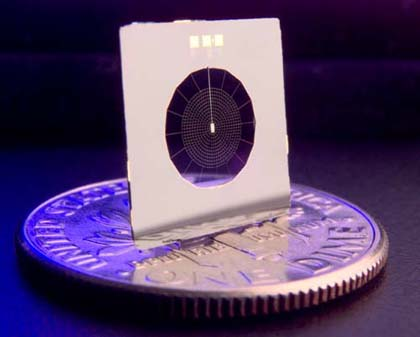
\includegraphics[width=80truemm]{slike/11_Bolometer.jpg}
\caption{Bolometer za merjenje prasevanja. Premer kovanca za primerjavo je 18~mm. 
Vir: NASA/JPL-Caltech.}
\label{fig:Bolometer}
\end{figure}

\subsection*{Termočlen}
Termočlen je sestavljen iz dveh različnih vodnikov. En spoj vodnikov počrnimo, drugega, 
referenčnega, pa zaščitimo pred svetlobo. Zaradi vpadne svetlobe se počrnjeni spoj 
segreje, med obema spojema nastane temperaturna razlika in zaradi termoelektričnega 
pojava tudi električna napetost, ki jo lahko merimo. Pri tem pazimo, da je prevodnost
vodnikov čim večja, toplotna prevodnost pa čim manjša. Odzivni čas termočlenov je 
okoli $\tau \sim 10$--$20~\si{\milli\second}$, občutljivost pa okoli $R \sim 10~\si{\volt/\watt}$.
Ker so napetosti, ki se pojavijo med stikoma, razmeroma majhne (le okoli 
$\sim 10~\si{\micro\volt/K}$) pogosto vežemo več (nekaj deset) termočlenov zaporedno v
termobaterijo. Občutljivost s tem naraste na $R \sim 200~\si{\volt/\watt}$, podaljša 
pa se časovna konstanta $\tau \sim 10$--$2000~\si{\milli\second}$. Prednost termočlenov je,
da za svoje delovanje ne potrebujejo zunanjega napajanja. 

\subsection*{Piroelektrični detektor}
Piroelektriki so snovi brez centra inverzije, v katerih je lastna električna 
polarizacija odvisna od temperature (npr. LiTaO$_3$, triglicin sulfat TGS 
in vsi feroelektriki). Piroelektrični detektor je narejen iz 
ploščice piroelektrične snovi med dvema elektrodama oziroma ploščama kondenzatorja.
Ko se ploščica zaradi absorbirane svetlobe segreje, se ji spremeni polarizacija in 
med elektrodama se pojavi premikalni tok, ki ga merimo na merilnem uporniku.

Zveza med spremembo temperature in spremembo polarizacije je
\beq
dP = a dT,
\eeq
kjer je $a$ piroelektrični koeficient. 

Med obema elektrodama s površino $S$ preteče naboj
\beq
de = I dt = S dP = S a dT.
\eeq
Tok skozi tipalo je tako
\beq
I = S a \frac{dT}{dt}.
\label{piro}
\eeq
Piroelektrični detektor je torej občutljiv na časovni odvod temperature detektorja, 
s tem pa tudi na spreminjanje vpadne svetlobne moči. V stacionarnem stanju 
detektor ne proizvaja električnega toka, zato moramo za merjenje 
konstantnega svetlobnega toka vpadno svetlobo najprej modulirati.
Navadno to naredimo kar z mehanskim zaklopom. Piroelektrični detektorji
se večinoma uporabljajo kot preprosti infrardeči detektorji. 
Njihova občutljivost je $R \sim 1~\si{\micro\ampere/\watt}$, odzivni čas pa odvisen od 
upornika v vezju, ampak lahko doseže vrednosti $\tau \sim 10~\si{\micro\second}$.

Poglejmo temperaturni odziv na tipalu. Izhajamo iz enačb~(\ref{TermTF}), (\ref{TermOdziv}) in
(\ref{piro}) in izračunajmo tok $I$ v odvisnosti od frekvence modulacije.
\beq
I = Sa \frac{dT}{dt} = Sa \frac{d}{dt} \int_{-\infty}^{\infty} T_\omega e^{i\omega t}d\omega 
=Sa\int_{-\infty}^{\infty}\frac{1}{\Lambda}\left(\frac{P_\omega}{1+i \omega \tau}\right) \,i \omega\,
e^{i\omega t}d\omega.
\eeq
Sledi 
\beq
I_\omega = \frac{i \omega\, SaP_\omega/\Lambda}{1 + i \omega \tau}.
\eeq
Vidimo, da pri majhnih frekvencah tok narašča, pri velikih frekvencah pa postane neodvisen od
frekvence modulacije vpadne svetlobe. Vendar to še ne pomeni, da lahko moduliramo s poljubno 
veliko frekvenco. Poleg relaksacijskega časa detektorja ima namreč karakteristični čas tudi
elektronsko vezje, ki določa zgornjo mejo za frekvenco. Ta je enak $\tau_e = R_eC_e$, pri čemer
sta $R_e$ upornost sistema in $C_e$ električna kapaciteta detektorja. 
\begin{figure}[h]
\centering
\def\svgwidth{65truemm} 
\input{slike/11_Piro.pdf_tex}
\caption{Spektralni odziv piroelektričnega detektorja na eni strani določajo toplotne izgube 
$\Lambda$ in toplotna kapaciteta detektorja $C$, navzgor pa odziv omejuje odziv elektronskega vezja $\tau_e$.}
\label{fig:Piro}
\end{figure}

\begin{definition}
Piroelektrični detektor naredimo iz kristala LiTaO$_3$ s koeficientom piroelektričnosti
$a = 2,3 \times 10^{-4}~\si{\ampere \second /\metre^2 \kelvin}$ in povprečno 
dielektričnostjo $\varepsilon = 50$. Izračunaj dovoljeno električno upornost sistema, 
če želimo, da detektor deluje za frekvence do 1~MHz. 
Dimenzija detektorja je $S = 1~\si{\centi\metre^2}$ in debelina $d = 1~\si{\milli\metre}$.
\end{definition}

\section{Fotoefekt}
Delovanje kvantnih detektorjev temelji na fotoefektu. To je pojav, pri katerem vpadli
fotoni iz snovi izbijajo elektrone. Izbiti elektroni lahko ubežijo kot prosti elektroni
(t. i. zunanji fotoefekt), ali pa ostanejo ujeti v snovi -- a mobilni -- in tako povečajo 
njeno prevodnost (notranji fotoefekt). V obeh primerih pride do fotoefekta le, 
če je energija vpadlih fotonov večja od neke določene energije.
Pod to vrednostjo fotoefekta ni, ne glede na moč vpadne svetlobe.
Fotoefekt je prvič opazil Hertz\footnote{Nemški fizik Heinrich Hertz, 1857--1894.} 
leta 1887, za njegovo razlago leta
1905 pa je Einstein\footnote{Nemški fizik in nobelovec Albert Einstein, 1879--1955.} 
dobil nobelovo nagrado. 

Poglejmo najprej zunanji fotoefekt, pri katerem elektron postane povsem prost. 
Da se to sploh lahko zgodi, mora biti energija vpadlega fotona dovolj velika, da 
elektron premaga potencialno bariero in izstopi iz prevodnega pasu (slika~\ref{fig:Nivoji}\,a). 
Najmanjšo energijo, ki je za to potrebna, imenujemo v kovinah izstopno delo. 
Če je energija fotona večja, gre preostanek energije v kinetično energijo izbitega
elektrona.

\begin{figure}[h]
\centering
\def\svgwidth{140truemm} 
\input{slike/11_Nivoji.pdf_tex}
\caption{Shema energijskih pasov in zunanjega fotoefekta v kovini (a) in polprevodniku (b) ter
notranjega fotoefekta v polprevodniku (c). $\Phi$ označuje izstopno delo, $E_g$ širino reže 
med valenčnim in prevodnim pasom poprevodnika,
$E_a$ pa elektronsko afiniteto. }
\label{fig:Nivoji}
\end{figure}

Zunanji fotoefekt poteka tudi v polprevodnikih (slika~\ref{fig:Nivoji}\,b). 
V tem primeru foton izbije elektron iz valenčnega pasu, njegova energija pa mora biti 
večja od vsote energije reže in elektronske afinitete, da lahko elektron zapusti snov. 
Z uporabo ustreznih materialov lahko dosežemo, da je elektronska afiniteta
negativna in je zato potrebna energija fotona kar enaka širini energijske reže.

Izstopno delo za kovine $\Phi$ je od okoli 2~eV za cezij pa do okoli 6~eV za platino. 
Ustrezna valovna dolžina svetlobe, ki še povzroči fotoefekt, je tako 
\beq
\lambda \leq \frac{hc}{\Phi},
\eeq
kar je 580~nm za primer cezija in samo okoli 200~nm za platino. Če želimo fotoefekt
izkostisti za detektorje vidne svetlobe, uporabimo druge snovi,
na primer Cs-Te, Cs-Sb, Na-K-Sb-Cs ali GaAs:Cs. 
Tako lahko zaznavamo fotone z valovnimi dolžinami od ultravijolične svetlobe 
pa vse do bližnje infrardeče. 

Pri notranjem fotoefektu (slika~\ref{fig:Nivoji}\,c) elektron snovi ne zapusti, ampak zgolj preide iz enega 
energijskega pasu v drugega. Tipično to poteka v polprevodnikih, kjer absorpcija fotona 
povzroči nastanek para elektron-vrzel, prag za nastanek para pa določa širina reže med 
energijskima nivojema. Primeri detektorjev, ki temeljijo na zunanjem fotoefektu, so 
fotocelice in fotopomnoževalke, na notranjem fotoefektu pa temeljijo na primer
fotoprevodniki, polprevodniške in plazovne fotodiode.

Za zdaj smo napisali, da fotoefekt poteče, ko foton izbije elektron. Vendar pri tem ni 
uspešen prav vsak foton, zato vpeljemo še en parameter, ki ga imenujemo kvantni izkoristek $\eta$.
Ta parameter pove verjetnost, da vpadli foton z valovno dolžino $\lambda$ oziroma frekvenco $\nu$ iz 
snovi izbije elektron. Električni tok, ki steče pri vpadni svetlobni moči $P$, je tako
\boxeq{11:eta}{
I = \eta e_0 n_F = \eta \frac{e_0 P}{h \nu},
}
kje je $n_F$ število vpadnih fotonov na časovno enoto.
Kvantni izkoristek je močno odvisen od valovne dolžine vpadne svetlobe in seveda
od snovi, na katero svetloba vpada. Za fotone z energijo, ki je manjša od izstopnega 
dela oziroma od širine energijske reže, je kvatni izkoristek praktično enak nič, 
nato pa strmo naraste in lahko doseže vrednosti, večje od $90~\%$. Podrobneje ga bomo 
obravnavali pri posameznih primerih detektorjev.

\begin{remark}
V praksi ločimo dve vrsti kvantega izkoristka: zunanji in notranji. Zunanji je vpeljan kot 
razmerje števila izbitih elektronov in fotonov, ki vpadejo na detektor. Ker pa se 
ob vpadu na detektor vedno nekaj fotonov odbije ali siplje, vpeljemo še notranji kvatni 
izkoristek kot razmerje števila elektronov in fotonov, ki se dejansko absorbirajo v detektorju.
Zunanji izkoristek je vedno manjši od notranjega in je neke vrste efektivni izkoristek.
\end{remark}

Iz enačbe(\ref{11:eta}) hitro izračunamo še občutljivost detektorja 
\boxeq{11:R}{
R = \frac{I}{P} = \frac{\eta e_0 }{h \nu}.
}

\section{Vakuumska fotodioda (fotocelica) in fotopomnoževalka}
\subsection*{Fotocelica}
Najpreprostejši kvantni detektor na zunanji fotoefekt je fotocelica ali vakuumska fotodioda
(slika~\ref{fig:Fotoefekt}). Fotocelica deluje tako, da svetloba vpada na katodo, 
zaprto v vakuumirani stekleni bučki, in tam povzroči fotoefekt. Izbite elektrone 
z zunanjo napetostjo pospešimo do anode in merimo električni tok, ki steče med 
katodo in anodo. Ker je tok sorazmeren s številom vpadlih fotonov, lahko na ta 
način izmerimo moč vpadne svetlobe.

\begin{figure}[h]
\centering
\def\svgwidth{60truemm} 
\input{slike/11_Fotoefekt.pdf_tex}
\caption{Shema fotocelice, v kateri poteka fotoefekt. 
Vpadna svetloba iz kovinske katode izbije elektrone, zaradi česar med katodo 
in anodo steče tok.}
\label{fig:Fotoefekt}
\end{figure}

Območje detekcije fotocelice je določeno z izstopnim delom kovine, iz katere fotoni izbijajo elektrone. 
Potrebno energijo fotona lahko precej zmanjšamo, če namesto čistih kovin uporabimo bi- ali 
večalkalne katode (npr. Na$_2$KSbCs), ali pa polprevodnike, na katere nanesemo tanko plast 
Cs ali Cs$_2$O. Tako ustvarimo negativno elektronsko afiniteto in izstopno delo je enako širini energijske
reže. Na ta način lahko zaznavamo svetlobo do valovnih dolžin okoli $1600~\si{\nano\metre}$. 
Na ultravijoličnem območju je delovanje
omejeno na okoli $160~\si{\nano\metre}$ zaradi neprepustnosti stekla, iz katerega je narejena bučka.
\begin{figure}[h]
\centering
\def\svgwidth{130truemm} 
\input{slike/11_SpekterKatode.pdf_tex}
\caption{Kvantni izkoristek fotocelic za različne snovi. Povzeto po Hamamatsu Photonics.}
\label{fig:Fotodioda}
\end{figure}

Čas odziva vakuumske fotodiode je odvisen od časa preleta elektronov od katode do anode. 
Da je ta čas čim krajši, je napetost na fotocelici pogosto več kV. Tedaj lahko dosežemo 
zelo kratke odzivne čase, tudi do 0,1~ns. Enostavnost in hitrost sta torej prednosti fotocelice, 
njena glavna pomanjkljivost pa je razmeroma nizek kvantni izkoristek. 
Ta je seveda močno odvisen od valovne dolžine vpadlega valovanja in snovi, iz 
katere je narejena katoda. Največje vrednosti, ki jih dosega, so okoli $40~\%$, 
pogosto pa več velikostnih redov manj. 
Vrednosti so razmeroma nizke, saj se izbiti elektroni gibljejo v vse
smeri in se pogosto sipljejo, preden sploh dosežejo površino. 

Dodaten problem fotocelic je, da pri končnih temperaturah prihaja do spontane oddaje elektrona.
Nekaj električnega toka zato teče tudi v popolni temi. To je rako imenovani temni 
tok fotodiode in tipično dosega vrednosti okoli $10^{-15}~\si{\ampere}$, lahko pa tudi do več nA. 
Za občutljive meritve je treba zato vakuumsko fotodiodo hladiti. 

\vskip1cm
\begin{definition}
Izračunaj občutljivost fotocelice na osnovi GaAs za valovanje z valovno dolžino $\lambda=620$~nm.
Pri tem kvantni izkoristek odčitaj s slike~(\ref{fig:Fotodioda}).
\end{definition}

\subsection*{Fotopomnoževalka}
Fotopomnoževalke so fotocelice z vgrajenim ojačenjem. Ojačenje dosežemo tako, da 
izbit fotoelektron najprej pospešimo z napetostjo $100$--$150~\si{\volt}$ na vmesno elektrodo, 
tako imenovano dinodo, iz katere izbije več ($\sim 5$--$10$, redkeje tudi do 40) 
sekundarnih elektronov. Ti elektroni
potujejo do naslednje dinode, ki je pod višjo pozitivno napetostjo (tipično okoli $100~\si{\volt}$
višjo), kjer ponovno izbijejo elektrone, ki vpadejo na naslednjo dinodo, ki je pod še višjo napetostjo ... 
To pomnoževanje se večkrat ponovi (navadno okoli desetkrat),
število elektronov eksponentno narašča in na en vpadli foton lahko dobimo $10^9$ elektronov na anodi. 
Občutljivost fotopomnoževalk je tako precej večja od občutljivosti vakuumske fotodiode in
dosega odzivnost na anodi do $R\sim 10^6~\si{\ampere/\watt}$.
Fotopomnoževalka tako omogoča štetje posameznih fotonov, po drugi strani pa moramo pri 
običajnih osvetlitvah paziti, da fotopomnoževalke ne osvetlimo preveč. 
\begin{figure}[h]
\centering
\def\svgwidth{80truemm} 
\input{slike/11_PMT.pdf_tex}
\caption{Shema fotopomnoževalke. Vpadna svetloba iz katode izbije elektrone, ti pa 
iz dinod izbijajo dodatne elektrone in izhodni signal se močno ojača.}
\label{fig:PMT}
\end{figure}

Fotopomnoževalke imajo zelo kratek odzivni čas, ki je odvisen od postavitve dinod. Posamezni 
elektroni do anode potujejo različno dolgo, zato je sunek na izhodu 
razširjen, tipično okoli $\sim 0,1$--$20~\si{\nano\second}$.  
Za manj zahtevne aplikacije pogosto merimo kar povprečni tok z anode. Kadar pa opazujemo
posamezne fotone, zaznamo na izhodu zaporedje sunkov. Takrat lahko 
amplituda izhodnega signala močno niha, saj je koeficient ojačenja 
odvisen od števila izbitih elektronov, kar pa je statistični proces. 

\section{Fotoprevodni detektorji}
Fotoprevodni detektorji\footnote{Fotoprevodne detektorje včasih imenujejo tudi fotouporniki.} 
so detektorji, ki temeljijo na notranjem fotoefektu.
Vpadli foton z dovolj veliko energijo se absorbira, vendar ne izbije elektrona v prostor, 
ampak ga iz valenčnega pasu dvigne v prevodnega. Pri tem nastane par elektron-vrzel. 
Ob priključeni napetosti se ti nosilci naboja začnejo premikati in steče tok, 
ki ga merimo. Z naraščajočim številom fotonov se prevodnost fotoprevodnika veča, 
zato lahko z merjenjem upornosti določimo 
intenziteto vpadle svetlobe. Tipično so fotoprevodniki iz polprevodnikov, 
lahko pa so tudi iz izolatorjev. 

Da foton lahko vzbudi elektron iz valenčnega v prevodni pas, mora biti njegova energija dovolj velika. 
V čistih (nedopiranih) polprevodnikih to pomeni, da mora biti energija fotona večja od 
širine reže. Za silicij, na primer, je širina reže 1,1~eV, s čimer lahko zaznavamo svetlobo
z valovno dolžino do okoli 
$1,1~\si{\micro\meter}$, za germanij 0,67~eV ($1,8~\si{\micro\meter}$) in za PbS 0,37~eV
($3,4~\si{\micro\meter}$). Za detekcijo daljših valovnih dolžin ne uporabljamo polprevodnikov
z manjšo energijsko režo, ampak dopirane polprevodnike (slika~\ref{fig:FPrevodnik}). 
Z novim energijskim nivojem med valenčnim in prevodnim pasom občutno zmanjšamo 
potrebno energijo vpadlih fotonov. Vendar je pri teh nizkih energijah prispevek termično 
vzbujenih elektronov že tako velik, da je treba detektorje hladiti, navadno s tekočim
dušikom ali celo tekočim helijem. Tak primer je germanij, dopiran s cinkom, 
s katerim lahko zaznavamo svetlobo do okoli $40~\si{\micro\meter}$. Pri tem ga hladimo
na $4~\si{\kelvin}$, da zmanjšamo pojav termično vzbujenih nosilcev naboja. 
\begin{figure}[h]
\centering
\def\svgwidth{150truemm} 
\input{slike/11_FPrevodnik.pdf_tex}
\caption{Shema prehoda elektrona v fotoprevodniku: prehod v čistem polprevodiku (a), 
$n$-dopiranem polprevodniku (b) in $p$-dopiranem polprevodniku (c). 
Z dopiranjem povečamo območje delovanja detektorja v infrardeče območje. }
\label{fig:FPrevodnik}
\end{figure}

Izračunajmo električni tok, ki steče, ko posvetimo na fotoprevodnik. Spomnimo se, da
je gostota električnega toka $j$ enaka vsoti prispevkov elektronov in vrzeli
\beq
j = e_0 n_v v_v + e_0 n_e v_e,
\eeq
pri čemer $n_v$ in $n_e$ pomenita gostoto vrzeli in elektronov v snovi, $v_v$ in $v_e$ pa 
hitrost vrzeli in elektronov. Ta je sorazmerna z električno poljsko jakostjo $E$, ki je priključena
 na vzorec, sorazmernostni faktor pa je gibljivost $\beta$. Ko posvetimo na vzorec, 
 se $n_v$ in $n_e$ povečata za $\Delta n_v$ in $\Delta n_e$,
gostota električnega toka pa naraste za
\beq
\Delta j = e_0 \Delta n_v v_v + e_0 \Delta n_e v_e.
\label{FP_j}
\eeq
V stacionarnem primeru se število nosilcev naboja ne spreminja in velja
\beq
0 = \frac{dn_v}{dt} = \frac{\eta_v P}{h \nu (Sl)} - \frac{\Delta n_v}{\tau_v}
\eeq
in podobno za elektrone. Pri tem je $\eta$ kvatni izkoristek, $P$ moč vpadne svetlobe,
$Sl$ prostornina detektorja in $\tau$ življenjski čas vrzeli oziroma elektrona. 
Ko stacionarno vrednost $\Delta n_v$ in $\Delta n_e$ vstavimo v enačbo~(\ref{FP_j}), dobimo
\beq
\Delta j = e_0 \frac{\eta_v P \tau_v}{h \nu (Sl)} \beta_v  E + 
e_0 \frac{\eta_e P \tau_e}{h \nu (Sl)} \beta_e  E.
\eeq
Če vpeljemo še napetost $U = E/l$, zapišemo celotni tok skozi fotoprevodnik zaradi vpadle svetlobe kot
\beq
\Delta I = \Delta j S = \frac{e_0 U P }{h \nu l^2} \left(\eta_v \tau_v \beta_v + 
\eta_e \tau_e \beta_e \right).
\eeq
Pogosto je gibljivost elektronov znatno večja od gibljivosti vrzeli (npr.
$0,135~\si{\meter}^2/\si{\volt\second}$ proti $0,048~\si{\meter}^2/\si{\volt\second}$ za silicij), 
zato prvi člen v oklepaju
zanemarimo in zapišemo
\beq
\Delta I = G \left( \frac{e_0 \eta_e}{h\nu}\right) P,
\eeq
pri čemer je koeficient ojačenja 
\beq
G = \frac{\beta_e \tau_e U}{l^2} = \frac{\tau_e}{\tau}.
\eeq
Vpeljali smo še čas preleta $\tau = v_e/l = \beta_e E/l = \beta_e U/l^2$.

Koeficient $G$ opiše ojačenje signala. Njegova vrednost je odvisna od 
vrste snovi in gibljivosti nosilcev naboja v njej, velikosti
detektorja in tudi priključene napetosti, zato lahko $G$ zavzane vrednosti od manj kot ena pa
vse do $10^6$. 

\begin{definition}
Izračunali smo spremembo toka, če fotoprevodnik osvetlimo s konstantno vpadno močjo. Pokaži, da
 je v primeru periodično spremenljive moči odziv enak
 \beq
\Delta I_\omega = G \left( \frac{e_0 \eta_e}{h\nu}\right) \frac{P_\omega}{1+i \omega \tau_e}.
 \eeq
 
\end{definition}

Fotoprevodniki so uporabni na širokem spektralnem območju, od ultra\-vijolične 
do daljne infra\-rdeče svetlobe. V vidnem in bližnjem infrardečem omočju se 
uporablja pretežno silicijeve fotoprevodnike, germanijeve
pa za valovne dolžine do $1,8~\si{\micro\meter}$. Za zaznavanje valovnih dolžin med okoli 
$2~\si{\micro\meter}$ in $7~\si{\micro\meter}$ so najprimernejši InAs, InSb in PbS detektorji, 
pri še daljših valovnih dolžinah pa se uporablja germanij, dopiran z zlatom, bakrom, cinkom, borom ...
Kvatni izkoristek takih detektorjev je razmeroma velik ($\eta = 0,5$ za Ge:Cu), vendar
je lahko faktor ojačenja $G \ll 1$ (npr. $G = 0,03$ za Ge:Hg). 

Hitrost odziva fotoprevodnika je odvisna od časa preleta nosilcev naboja,
ki je določen z geometrijo detektorja, in od karakterističnega časa elektronskega vezja. 
Tipični odzivni časi so okoli mikrosekunde, vendar lahko sežejo
tudi do desetin milisekund, ali pa v izjemnih primerih do nanosekund za zelo majhne detektorje.
S skrajšanjem rekombinacijskega časa lahko sicer skrajšamo odzivni čas detektorja, 
vendar hkrati zmanjšamo tudi njegovo občutljivost.

\begin{remark}
Fotoprevodni detektorji so narejeni iz zelo tankih plasti fotoprevodnika, saj močno absorbira
svetlobo. Tako za absorpcijo $70-90\%$ svetlobe zadošča le $1$--$2~\si{\micro\meter}$ debela plast.
Elektrode se pogosto prepletajo, da se zmanjša dolžina preleta $l$ in poveča ojačenje $G$. 
\end{remark}

\section{Polprevodniške fotodiode}
Drugi primer detektorjev, ki temeljijo na notranjem fotoefektu, so polprevodniške fotodiode.
Te so danes najpogostejša in najbolj razširjena vrsta detektorjev svetlobe, uporabljamo jih med
drugim tudi v fotoaparatih in sončnih celicah. Fotodiode so sestavljene iz $p$- in $n$-dopiranega 
polprevodnika ($p$-$n$ fotodiode) ali pa je med njima še plast nedopiranega (intrinzičnega) 
polprevodnika ($p$-$i$-$n$ fotodioda). Ko svetloba vpade na $p$-$n$ (ali $p$-$i$-$n$) 
stik, se fotoni absorbirajo in nastajajo 
pari elektron-vrzel. Nosilci naboji potujejo v različnih smereh, elektroni stečejo v eno smer,
vrzeli pa v nasprotno. Odvisno od načina delovanja lahko izmerimo tok, ki steče skozi 
stik, ali pa napetost, ki se pojavi na stiku. 

Spektralni odziv fotodiod je seveda odvisen od energijske reže polprevodnika, 
iz katerega je fotodioda narejena.
Silicijeve fotodiode so tako uporabne za zaznavanje valovnih dolžin do okoli
$1,1~\si{\micro\meter}$, za
večje valovne dolžine (do $1,6~\si{\micro\meter}$) uporabljamo InGaAs. Izkoristek fotodiod
je navadno zelo velik in presega $50~\%$, pri energiji fotonov blizu energijske reže 
je vrednost izkoristka kar blizu 1.
Za razliko od fotoprevodnikov fotodiode signala
ne ojačujejo, imajo pa praviloma hitrejši odziv, tipično okoli nanosekunde.

Dioda lahko deluje v različnih načinih (slika~\ref{11_PD}). 
Lahko jo priključimo v prevodni smeri, najpogosteje jo priključimo v zaporni smeri, saj je v
tem primeru tok skozi diodo linearno sorazmeren z intenziteto vpadne svetlobe, lahko 
je dioda kratko sklenjena, lahko pa je dioda v odprtem električnem krogu, v t.i. fotovoltaičnem 
načinu. V nadaljevanju bomo vse primere podrobneje spoznali.
\begin{figure}[h]
\centering
\def\svgwidth{140truemm} 
\input{slike/11_diode.pdf_tex}
\caption{Različne vezave fotodiode: v prevodni smeri (a), v zaporni smeri (b), kratko sklenjena (c) in 
v fotovoltaičnem načinu (d)}
\label{11_PD}
\end{figure}

\subsection*{Stik $pn$}
Ponovimo najprej, kaj se zgodi ob stiku $p$- in $n$- tipa polprevodnika. Pri tem tip $p$ označuje
polprevodnik, dopiran s trivalentnimi akceptorskimi primesmi, ki v snovi ustvarijo vrzeli.
Energijski nivo primesi je malo nad vrhom valenčnega pasu, zato je Fermijeva energija
polprevodnika premaknjena navzdol proti valenčnem pasu (slika~\ref{11_PN1}\,a). 
Po drugi strani $n$ tip označuje polprevodnike s petvalentnimi 
donorskimi primesmi, ki v snov prinesejo dodatne elektrone. Njihov energijski nivo je malo 
pod prevodnim pasom, zaradi česar je Fermijeva energija pomaknjena navzgor proti prevodnemu pasu
(slika~\ref{11_PN1}\,b).

Ko staknemo polprevodnik tipa $p$ s polprevodnikom tipa $n$, elektroni 
z območja z višjo koncentracijo (tip $n$) difundirajo v območje z nižjo koncentracijo
(tip $p$), kjer se rekombinirajo z vrzelmi. 
Ob stiku tako nastane ozek pas,  imenujemo ga izpraznjeni sloj, kjer ni več 
prostih nosilcev naboja. Ostanejo pa pozitivno nabiti donorski atomi na strani $n$
in negativno nabiti akceptorski atomi na strani $p$. Ti naboji povzročijo nastanek  
električnega polja, ki kaže od $n$ proti $p$. Nastalo polje zaustavi rekombinacijo, saj odbija
elektrone in vrzeli od stika. V ravnovesju se Fermijeva energija izenači, potencialni
skok pa je približno enak $\Delta E \approx E_d-E_a$, kar je le malo manj od 
širine reže $E_g$ (slika~\ref{11_PN1}\,c).

\begin{figure}[h]
\centering
\def\svgwidth{140truemm} 
\input{slike/11_PN1.pdf_tex}
\caption{Shema energijskih nivojev v $p$- (a) in $n$-tipu (b) polprevodnika ter na $p$-$n$ stiku (c), 
v katerem se Fermijevi energiji izenačita. Med obema polprevodnikoma nastane izpraznjeni sloj, kar 
povzroči nastanek električnega polja.}
\label{11_PN1}
\end{figure}

\begin{figure}[h]
\centering
\def\svgwidth{140truemm} 
\input{slike/11_PNU.pdf_tex}
\caption{Shema energijskih nivojev v $p$-$n$ stiku, ko na stik priključimo napetost
v prevodni smeri (a) in v zaporni smeri (b). Če v izpraznjenem sloju pride do absorpcije
fotona in nastanka para elektron-vrzel, elektron ``zdrsi'' proti strani $n$, vrzel pa proti
strani $p$.}
\label{11_PNU}
\end{figure}

Priključimo zdaj na diodo napetost, tako da je pozitivna na $p$ strani diode. Takrat 
pravimo, da smo na diodo priključili napetost v prevodni smeri. Ker lahko energijske
pasove razumemo kot potencialno energijo elektronov, s priključeno napetostjo
zmanjšamo razliko potencialnih energij in elektroni lažje prehajajo iz $n$ v $p$ del. 
Zaradi zmanjšanja potencialne razlike med $p$ in $n$ stranjo za $e_0U$ pride do povečanja toka 
večinskih elektronov iz $n$ v $p$ za faktor $\exp(e_0 U/kT)$, tok manjšinskih elektronov
iz $p$ v $n$ pa ostaja enak, saj ni ovisen od globine potencialnega skoka 
(slika~\ref{11_PNU}\,a). 

Povsem enak razmislek lahko naredimo, če priključimo 
na $n$ stran pozitivni pol, na $p$ stran pa negativnega, če torej priključimo
napetost v zaporni smeri. V tem primeru potencialna razlika naraste in tok 
večinskih elektonov se zmanjša za faktor $\exp(-e_0 |U|/kT)$, tok 
manjšinjskih elektronov pa ostane nespremenjen (slika~\ref{11_PNU}\,b).

Celotni tok skozi $p$-$n$ stik je sestavljen iz prispevkov elektronov in vrzeli, 
opiše pa ga tako imenovana karakteristična enačba diode (slika~\ref{11_IU})
\boxeq{11:dioda}{
I = I_0 (e^{e_0 U/kT}-1).
}
Pri tem $I_0$ označuje tok manjšinskih nosilcev naboja\footnote{Pravimo
mu tudi zaporni tok, tok nasičenja ali temni tok. Slednje ime sledi iz tega, da
ta tok teče skozi fotodiodo tudi v odsotnosti svetlobe.}
in je navadno zelo majhen. Njegova vrednost je odvisna od snovi, površine
detektorja, poleg tega pa je eksponentno odvisna od temperature. Znaša 
tipično okoli $10^{-5}$-$10^{-15}~\si{\ampere}$, pri čemer najmanjše
vrednosti dosegamo le ob močnem hlajenju. 

\begin{figure}[h]
\centering
\def\svgwidth{100truemm} 
\input{slike/11_IU.pdf_tex}
\caption{$I(U)$ karakteristika neosvetljene fotodiode (modra črta)
in osvetljene fotodiode (rdeče črte). Naraščajoča intenziteta vpadne svetlobe
krivuljo premakne navzdol. S simboli so označene točke delovanja za različne načine.
}
\label{11_IU}
\end{figure}
 
\subsection*{Delovanje fotodiode}
Ko na polprevodnik vpade foton, ki ima energijo večjo od širine reže, 
lahko vzbudi elektron iz valenčnega v prevodni pas in nastane par elektron-vrzel. 
Če se to zgodi v izpraznjenem sloju $p$-$n$ stika, steče elektron pod vplivom 
električnega polja na stran $n$, vrzel pa na stran $p$ (slika~\ref{11_PNU}\,c). 
Premik nosilcev naboja, do katerega je prišlo zaradi absorpcije fotona, 
torej vedno steče v zaporni smeri. 
Njegova velikost je odvisna od moči vpadne svetlobe in jo lahko zapišemo kot  
\boxeq{11:if}{
I_f = e_0 \eta n_F = e_0 \frac{\eta P}{h \nu},
}
pri čemer smo z $n_F$ onačili število vpadnih fotonov na časovno enoto, 
$\eta$ je kvantni izkoristek,
$P$ pa označuje moč vpadne svetlobe. Celoten tok skozi fotodiodo je kombinacija diodnega 
in svetlobnega toka, zato karakteristiko fotodiode zapišemo kot 
\boxeq{11:fotodioda}{
I = I_0 (e^{e_0 U/kT}-1) - I_f.
}
Vpadna svetloba torej povzroči zmanjšanje električnega toka skozi diodo, 
kar na sliki~(\ref{11_IU}) predstavlja premik karakteristike diode v vertikalni 
smeri (rdeče črte). Naraščajoča intenziteta svetlobe premika krivuljo proti 
bolj negativnim vrednostim tokov. 

Prvi način delovanja fotodiode, ki ga bomo obravnavali, je {\bf fotovoltaični način}.
To je način, pri katerem električni tokokrog ni sklenjen (slika~\ref{11_PD}\,d), 
zato ob absorpciji fotona in nastanku
para elektron-vrzel tok ne more steči. Še vedno pa se izbiti elektron pod vplivom električnega polja
na stiku premakne proti $n$ delu, vrzel pa proti $p$. Na diodi se tako pojavi napetost, 
katere vrednost lahko izračunamo iz karakteristične enačbe diode, če upoštevamo, da je $I=0$. Sledi
\beq
U_p = \frac{kT}{e_0}\ln \left(1+ \frac{I_f}{I_0}\right).
\eeq
Pri večji intenziteti vpadle svetlobe, ko se krivulja na grafu (\ref{11_IU}) pomika navzdol, se rešitev
gornje enačbe po abscisi premika proti desni. Večja intenziteta vpadne svetlobe torej pomeni večjo 
pozitivno napetost na diodi, zato tudi odzivnost v tem primeru merimo v $\si{\volt}/\si{\watt}$.
Pri dovolj velikih vpadnih močeh je zveza med vpadno močno in fotonapetostjo
logaritemska. Taka vezava fotodiode tako omogoča zaznavanje vpadne moči v zelo širokem intervalu,
najpogosteje pa se ta način delovanja uporablja v sončnih celicah. 

Drugi način delovanja je {\bf kratko sklenjena} fotodioda (slika~\ref{11_PD}\,c). V tem primeru je 
napetost na diodi enaka nič in je tok skozi tokokrog kar enak toku zaradi vpadle svetlobe $I_f$
(slika~\ref{11_IU}).

Najbolj splošno uporabljen način za detekcijo svetlobe je način, v katerem napetost na diodo 
priključimo {\bf v zaporni smeri} (slika~\ref{11_PD}\,b).
Takrat se tok skozi diodo spreminja linearno z močjo vpadne svetlobe, odziv pa je hitrejši
kot pri kratko sklenjeni diodi. Če dodamo v tokokrog zaporedno vezan še nek upornik, se odziv
spremeni. Po grafu (slika~\ref{11_IU}) se ne premikamo več navzdol, ampak pod kotom proti desni.
Enačbo, ki opisuje premico, ki seka karakteristične krivulje, lahko preprosto zapišemo
z Ohmovim zakonom $U = -|U_0|-RI$. 

Prednosti tega načina merjenja je več. Zaradi priključene napetosti se zmanjša čas preleta
nosilcev naboja in posledično se zmanjša odzivni čas detektorja. Dodatno se poveča
širina izpraznjenega pasu, kar zmanjša kapaciteto stika (stik $p$-$n$ namreč deluje kot neke vrste 
kondenzator in časovni odziv je odvisen od njegove kapacitete) in s tem odzivni čas. Povečana
izpraznjena plast pa vodi do večjega območja, v katerem lahko pride do absoprcije fotonov. 

Povejmo še nekaj o zgradbi fotodiode. Shema preproste fotodiode je prikazana na sliki~(\ref{11_shema}\,a).
Na dnu je elektroda, sledi plast $n$, nad njo je tanka plast $p$, na katero vpada svetloba.
Bistveno je, da je osvetljena plast tanka, da svetloba lahko prodre v bližino stika. Zato so 
debeline zgornje plasti tipično submikronske. Dodatno na fotodiode pogosto nanesemo
še dodatno antirefleksijsko plast (SiO$_2$). Fotoobčutljiv del komercialnih fotodiod
je tipično od nekaj $100~\si{\micro\meter}^2$ pa do več $100~\si{\milli\metre}^2$. Pri 
tem imajo večje diode seveda počasnejši odziv. 

\begin{remark}
Poleg do zdaj obravnavanih fotodiod, poznamo tudi heterostrukturne fotodiode, kjer sta $p$ in $n$ del
narejena iz druge snovi. Poseben primer so Schottkyjeve fotodiode, kjer eno plast polprevodnika
nadomestimo z zelo tanko plastjo kovine (slika~\ref{11_shema}\,c). Te so uporabne predvsem pri 
visokih energijah (v UV območju), 
saj je v navadnih fotodiodah absorpcija za te valovne dolžine prevelika, na površini pride do 
rekombinacije in zmanjšanja kvantnega izkoristka. Poleg tega je odziv Schottkyjevih fotodiod zelo hiter, 
ker nizka upornost kovine občutno zmanjša $RC$ konstanto stika. Odzivni časi dosegajo pikosekundne vrednosti. 
\end{remark}

\begin{figure}[h]
\centering
\def\svgwidth{140truemm} 
\input{slike/11_shema.pdf_tex}
\caption{Shema $p$-$n$ fotodiode (a), $p$-$i$-$n$ fotodiode, ki se od navadne 
$p$-$n$ razlikuje po vmesni plasti intrinzičnega
polprevodnika (b) in shema Schottkyjeve fotodiode (c)}
\label{11_shema}
\end{figure}

\subsection*{Fotodioda $pin$}
Fotodiode $p$-$i$-$n$ se od navadnih $p$-$n$ razlikujejo po tem, da med $p$- in $n$-plast 
vključimo še plast nedopiranega polprevodnika (slika~\ref{11_shema}\,b). S tem se efektivno bistveno poveča območje
izpraznjene plasti in njegova širina postane praktično neodvisna od priključene napetosti.
Povečanje izpraznjene plasti omogoča zaznavanje bistveno večjega deleža vpadne svetlobe, 
poleg tega pa zmanjša kapaciteto stika in s tem njegovo $RC$ konstanto. Slabost dodatnega
sloja je povečanje časa preleta čez izpraznjeno plast, vendar lahko
z ustrezno optimizacijo konstrukcije dosežemo odzivne čase nekaj deset ps.

\begin{figure}[h]
\centering
\def\svgwidth{100truemm} 
\input{slike/11_SpekterFD.pdf_tex}
\caption{Kvantni izkoristek nekaterih $p$-$i$-$n$ in Schottkyjevih fotodiod.}
\label{11_odziv}
\end{figure}

\section{Plazovne fotodiode}
Ko smo risali karakteristiko fotodiode, nismo narisali popolne slike. 
Pri velikih negativnih napetostih se namreč karakteristika znatno spremeni (slika~\ref{11_plaz}), 
česar ne moremo popisati s preprosto enačbo. Pri zapornih napetostih, ki za nekajkrat presegajo 
širino energijske reže (tipično okoli $10^7~\si{\volt}/\si{\meter}$), 
pride do naglega povečanja električnega toka. Ob absopciji fotona nastali
mobilni nosilci naboja se namreč v električnem polju tako pospešijo, da s trki ustvarjajo nove pare 
elektron-vrzel. Ti novonastali pari ponovno ustvarjajo pare in pride do ``plazu'', podobno kot v 
fotopomnoževalki. En foton torej sproži cel plaz elektronov, zato pravimo, da je plazovna dioda
fotodioda z notranjim ojačenjem. Pri tem je faktor ojačenja tipično $30$-$300$ in jih lahko 
uporabimo za detekcijo posameznih fotonov. Slabost je, da je faktor ojačenja odvisen od
temperature in je zato za natančne meritve potrebna temperaturna stabilizacija.

Napetost, pri kateri deluje plazovna fotodioda, je priključena v zaporni smeri jih jo 
držimo tik pod prebojno napetostjo. Ker že  majhna odstopanja v napetosti povzročijo veliko
spremembo v toku, moramo tudi napetost držati kar se da stabilno. Le to omogoča
linearen odziv fotodiode od moči vpadne svetlobe. Take fotodiode so praviloma zelo hitre 
($50~\si{\pico\second})$ in zelo občutljive. Z ojačenjem signala se ojača tudi šum, a je ta 
porast pogosto manjša kot bi bil prispevek k šumu na zunanjih elektonskih ojačevalcih. 

\begin{figure}[h]
\centering
\def\svgwidth{60truemm} 
\input{slike/11_plaz.pdf_tex}
\caption{Karakteristika plazovne fotodiode}
\label{11_plaz}
\end{figure}

\section{CCD in CMOS detektorji}
Do zdaj smo obravnavali detektorje, ki zaznavajo pretok vpadnih fotonov in spreminjanje
tega pretoka s časom. Dodatno informacijo dobimo, če več fotodetektorjev sestavimo v 
dvodimenzionalno matriko, saj lahko ti detektorji hkrati zaznavajo količino vpadne svetlobe 
iz različnih delov prostora in dobljene podatke sestavimo v sliko. Pri tem en detektor
podaja informacijo o številu vpadnih fotonov v dani časovni enoti (integracijski čas
oziroma čas osvetlitve) en slikovni 
element -- piksel. Slikovni detektorji z veliko ločljivostjo so tako sestavljeni iz 
več milijonov ali celo milijarde posameznih polprevodniških detektorjev in so 
nepogrešljivi v fotoaparatih, video-kamerah, mikroskopiji in astronomiji.

Podrobneje bomo obravnavali dva primera matričnih detektorjev, to so CCD 
({\it charge-coupled-device})\footnote{Za izum CCD detektorjev sta Willard 
S. Boyle in George E. Smith  leta 2009 prejela Nobelovo nagrado.} 
in CMOS ({\it complementary metal-oxide-semicoductor})
\footnote{Teh dveh oznak za detektorje praviloma ne prevajamo. Opisujeta 
strukturo in delovanje naprave in nista vezani zgolj na detekcijo svetlobe.}. Obe vrsti
detektorjev sta si glede zaznavanja svetlobe zelo pododbni, razlika
je predvsem v načinu, kako iz posameznega detektorja dobimo podatek o številu 
vpadlih fotonov oziroma številu vzbujenih elektronov.

\begin{remark}
Slikovni detektorji so seveda lahko sestavljeni tudi iz drugih svetlobnih detektorjev, 
ki smo jih obravnavali v prejšnjih razdelkih. Lahko so iz mikrobolometrov
ali fotoprevodnikov (za IR svetlobo), Schottkyjevih fotodiod (npr. PtSi, ki seže od UV do
okoli $6~\si{\micro\meter}$) ali plazovnih fotodiod.
\end{remark}

\subsection*{CCD}
Detektorjev CCD so sestavljeni iz posameznih tako imenovanih MOS ({\it metal-oxide-semiconductor}
-- kovina-oksid-polprevodnik) kodenzatorjev. Njihova osnova je dopiran silicij, vmesna 
plast med polprevodnikom in prevodno elektrodo pa je navadno zelo tanka plast (pod 100 nm)
SiO$_2$ (slika~\ref{11_MOS}).
Prevodna elektroda je bila prvotno iz kovine (npr. aluminija) in je elementu detektorja dala tudi ime.
Danes je kovino večinoma nadomestil polikristalni silicij (polisilicij), ime pa je ostalo.
Tipična dolžina stranice posameznega elementa znaša okoli $5$-$40~\si{\micro\meter}$. 
\begin{figure}[h]
\centering
\def\svgwidth{140truemm} 
\input{slike/11_MOS.pdf_tex}
\caption{Shema MOS strukture (a), ki je osnova za vse CCD in CMOS slikovne detektorje. Osnova je 
polprevodnik ($p$), na katerem je plast dielektrika (SiO$_2$), na njej pa elektroda (siva). 
Ob absorpciji svetlobe se pojavijo fotoelektroni, katere pozitivna napetost
na elektrodi drži ujete v potencialno jamo (vijolična). Prenos elektronov v CCD detektorju (b).}
\label{11_MOS}
\end{figure}

Ko foton vpade na element MOS skozi tako prozorno elektrodo, v polprevodniku ustvari
par elektron-vrzel. Pozitivna napetost na elektrodi elektrone privlači, vendar jih 
vmesna plast izolatorja tik pod površino ustavi in elektroni tako ostanejo ujeti v potencialni jami. 
Pri tem je število ujetih elektronov sorazmerno številu vpadlih fotonov v času zajemanja slike, 
pomnoženih s kvantnim izkoristkom pri dani valovni dolžini. 

S spreminjanjem napetosti na posameznih elektrodah lahko naboj, ki se lokalno nabere 
v plasti pod izolatorjem v danem času, postopoma prenesemo od posameznega 
piksla do izhodne stopnje. Najprej poteka prenos iz enega elementa na drugega v eni vrstici, 
nato pa še po celotnem stolpcu (slika~\ref{11_CCD}\,a). Na koncu signal sproti ojačujemo, 
pretvorimo v napetost, to pa v digitalni zapis. Pri tem številu elektronov iz posameznega
slikovnega elementa določimo digitalno vrednost glede na barvno globino. 8-bitni zapis slike
tako vsakemu elementu priredi vrednost od 0 do 255, 16-bitni pa od 0 do 65535.

Delovanje detektorjev CCD torej temelji na zaporednem odčitavanju števila fotoelektronov v posameznem 
slikovnem elementu. Ta način je razmeroma počasen in omejuje hitost zajemanja slike. Med 
prenašanjem nabojev do izhoda namreč slike ne moremo zajemati, saj bi prišlo do popačenja signala. 
Ta problem se večinoma rešuje tako, da le del celotnega zaslona zajema svetlobo, drug del
pa je namenjen pretakanju elektronov in omogoča nemoteno praktično neprestano zajemanje slike.
Ker se s tem količina zajete svetlobe zmanjša, se na vsak element doda lečo, ki svetlobo zbere
na detektor. S tem postanejo slikovni detektorji CCD hitrejši in bolj občutljivi. Poleg
tega jih odlikuje tudi razmeroma nizek šum, ki se ga da s hlajenjem še dodatno 
zmanjšati. 

\begin{remark}
Pogosto pri eksperimentu ne potrebujemo največje možne ločljivosti, ki jo nudi detektor. 
Takrat se pogosto poslužujemo združevanja sosednjih elementov, t. i. bininga, na primer $2\times2$
ali $4\times4$, in s tem sicer zmanjšamo ločljivost, ampak hkrati skrajšamo čas
zajemanja slike in zmanjšamo razmerje signal proti šumu. 
\end{remark}

\begin{figure}[h]
\centering
\def\svgwidth{80truemm} 
\input{slike/11_CCD.pdf_tex}
\caption{Shema CCD (a) in shema CMOS (b) slikovnega detektorja. Puščice označujejo premikanje
fotoelektronov.}
\label{11_CCD}
\end{figure}

\subsection*{CMOS}
Osnovni element detektorjev CMOS je enak kot za detektorje CCD (slika~\ref{11_MOS}\,a). 
Bistvena razlika je v načinu zajemanja fotoelektronov. Pri detektorjih CCD je bilo branje 
fotoelektronov zaporedno, pri detektorjih CMOS pa poteka branje vseh slikovnih elementov 
hkrati, pri čemer ima vsak piskel tudi svoj ojačevalnik (slika~\ref{11_CCD}\,b).
Zaradi sprotnega odčitavanja vseh pikslov naenkrat so detektorji CMOS bistveno hitrejši 
od CCD. Odlikuje jih tudi nizka poraba energije in nizka cena. Njihova poglavitna slabost
je večji šum in manjša občutljivost, saj del zaslona, kjer so ojačevalniki, slike ne more
zajemati. 

\subsection*{Barvno zajemanje slik}
Detektorji zaznavajo samo število vpadlih fotonov oziroma bolj natančno število fotoelektronov.
Za nastanek barvne slike moramo vpadle fotone ločiti še po valovni dolžini, kar naredimo
z barvnimi filtri. Namesto enega elementa, ki bi podal informacijo o intenziteti vpadne 
svetlobe, imamo štiri senzorje v kvadratni mreži, rdečega, modrega in dva zelena. 
Večji delež zelenih elementov je zaradi večje občutljivosti človeškega očesa na zeleno barvo. 
Intenziteto svetlobe na posameznem slikovnem elementu dane barve nato odčitamo kot je
opisano zgoraj.
 
\section{Šum pri optični detekciji}
Pri vsakršni detekciji svetlobe je vedno prisoten tudi šum. Beseda šum označuje naključne 
fluktuacije na izhodu iz detektorja, ki jih ne moremo ločiti od signala. Z različnimi 
pristopi lahko šum zmanjšamo, povsem ga pa ne moremo nikoli odpraviti. Obravnava 
šuma je zato najbolj pomembna pri zaznavanju šibkih signalov svetlobe. Pri tem je ključen
parameter najmanjša moč vpadne svetlobe, ki jo še lahko ločimo od šuma, pod to vrednostjo 
pa se signal v šumu izgubi (slika~\ref{11_sum}).
\begin{figure}[h]
\centering
\def\svgwidth{140truemm} 
\input{slike/11_sum.pdf_tex}
\caption{Če je signal velik v primerjavi s šumom, ga na detektorju lahko zaznamo (zgoraj). 
Pod določeno vrednostjo postane velikost signala primerljiva s šumom in signala ne zaznamo več
(spodaj).}
\label{11_sum}
\end{figure}

Na podlagi fizikalnega izvora ločimo več vrst šuma:
\begin{enumerate}
\item šum štetja, do katerega pride zaradi diskretne (kvantne) narave fotonov,
\item termični šum, do katererega pride zaradi termičnih fluktuacij,
\item šum temnega toka, ki predstavlja spontani nastanek para elektron-vrzel oziroma spontano
emisijo elektronov in
\item šum sevanja ozadja.
\end{enumerate}

\subsection*{Šum štetja} 
Ko govorimo o svetlobi, ne smemo pozabiti, da je svetloba sestavljena iz diskretnih fotonov. 
Fotoni vpadajo na detektor posamezno in enkrat jih vpade malo več, 
drugič malo manj. Vpadna moč je zato dejansko povprečna moč $\overline{P}$ in število 
vpadlih fotonov na časovno enoto je povprečna vrednost števila vpadlih fotonov na časovno enoto
\beq
\overline{n} = \frac{\overline{P}}{h\nu}.
\eeq
Pri vpadu fotonov gre za diskretne in neodvisne procese, zato za njihov vpad velja
Poissonova porazdelitev (slika~\ref{11_Poiss}). Verjetnost, da v času $\tau$, ki prestavlja 
čas merjenja, na detektor vpade $N$ fotonov, je tako 
\beq
p(N) = \frac{\overline{N}^N e^{-\overline{N}}}{N!},
\label{Poisson}
\eeq
pri čemer je povprečno število vpadlih fotonov v tem časovnem intervalu 
enako $\overline{N} = \overline{n}\tau$.
\begin{figure}[h]
\centering
\def\svgwidth{90truemm} 
\input{slike/11_poisson.pdf_tex}
\caption{Poissonova porazdelitev verjetnosti za $\overline{N}=2$ (modra), 
$\overline{N}=5$ (rdeča) in $\overline{N}=10$ (zelena). Porazdelitev je 
diskretna, črta je zgolj vodilo.}
\label{11_Poiss}
\end{figure}

Fluktuacije števila fotonov, ki vpadejo na detektor v danem časovnem 
intervalu, označimo z $\Delta N = N-\overline{N}$. V povprečju je ta vrednost seveda enaka nič, 
zato sta bolj merodajni količini varianca, ki je enaka (glej nalogo~\ref{nal:Poiss})
\beq
\sigma^2 = \overline{\Delta N^2}= \overline{(N-\overline{N})^2} = \overline{N},
\label{varianca}
\eeq
in standardni odklon
\beq
\sigma = \sqrt{\overline{\Delta N^2}} = \sqrt{\overline{N}}.
\label{sigma}
\eeq
\begin{definition}
Pokaži, da je povprečje Poissonove porazdelitve (enačba~\ref{Poisson}) vedno pri $N = \overline{N}$
in standardni odklon $\sigma = \sqrt{\overline{N}}$.
\label{nal:Poiss}
\end{definition}

Standardni odklon, ki je merilo za velikost šuma, torej narašča z naraščajočim številom 
vpadnih fotonov $\overline{N}$. Vendar nas absolutni šum večinoma ne zanima, 
saj je pri detekciji ključno razmerje 
signala proti šumu. To količino označimo s $SNR$ ({\it Signal to Noise Ratio}-- razmerje med 
signalom in šumom)\footnote{Pogosto se uporablja tudi oznako $S/N$. Tukaj smo jo 
zaradi jasnosti zamenjali, saj $N$ označuje število fotonov oziroma elektronov.}. 
V primeru Poissonove porazdelitve in šuma štetja velja
\boxeq{11:SNR}{
SNR = \frac{\overline{N}}{\sigma} = \sqrt{\overline{N}}.
}
Vidimo, da razmerje signala proti šumu narašča z naraščajočim številom vpadlih fotonov, 
relativni šum pa ob večji vpadni moči svetlobe pojema. Za primer poglejmo dva primera vpadne svetlobe. 
V prvem je povprečno število vpadlih fotonov v danem časovnem 
intervalu $10^6$, v drugem pa le $100$. Pri vpadu močnejšega signala 
na detektorju zaznavamo $10^6 \pm 1000$ fotonov, pri vpadu šibkejšega
pa $100 \pm 10$. Čeprav je absolutni šum v prvem primeru znatno večji, 
je relativni šum stokrat manjši. Za zmanjšanje šuma štetja mora biti 
torej signal kar se da velik. 

Pri šumu štetja gre za osnovno značilnost svetlobe, zato je ta vrsta šuma
prisotna pri prav vseh načinih detekcije. Mi si podrobeneje oglejmo, 
kako se ta šum izraža pri detekciji s fotodiodami. 

Naj svetloba s povprečno močjo $\overline{P}$ vpada na fotodiodo.
Povprečno število fotoelektronov, ki se pojavijo v časovnem intervalu 
$\tau$, je kar enako številu vpadlih fotonov, pomnoženim 
s kvantnim izkoristkom. 
\beq
\overline{N}_e = \frac{\overline{P}\tau}{h \nu}\eta.
\eeq
Povprečni tok, ki steče skozi detektor, je  
\beq
\overline{I} = \frac{\overline{N}_e e_0}{\tau},
\eeq
fluktuacije izhodnega električnega toka pa so
\beq
\overline{\Delta I^2}=\overline{(I-\overline{I})^2} = \overline{(N_e-\overline{N}_e)^2}\,
\frac{e_0^2}{\tau^2} = \overline{N}_e\,\frac{e_0^2}{\tau^2}= \overline{I}\,\frac{e_0}{\tau},
\eeq
pri čemer smo upoštevali enačbo~(\ref{varianca}). Vpeljemo še pasovno širino 
detekcije $\Delta\nu_B = 1/(2\tau)$ in dobimo
\boxeq{11:sum}{
\sqrt{\overline{\Delta I^2}} = \sqrt{2 \overline{I}\,e_0\, \Delta\nu_B}.
}
Šum na izhodu je torej sorazmeren s korenom iz povprečne intenzitete signala in 
s korenom od pasovne širine detekcije oziroma obratno sorazmeren z dolžino 
merjenja. Zapišemo še razmerje signala proti šumu 
\beq
SNR = \frac{\overline{I}}{\sqrt{\overline{\Delta I^2}}}= \frac{\sqrt{\overline{I}}}
{\sqrt{2 e_0\, \Delta\nu_B}}.
\label{SNRs}
\eeq
Po pričakovanjih je to razmerje večje pri večjem povprečnem signalu in pri daljši meritvi.

\begin{remark}
Razmerje signal proti šumu $SNR$ lahko vpeljemo na več načinov. Prvi je ta, ki smo ga 
uporabili mi, pri katerem velja $SNR = \overline{N}/\sigma = \sqrt{\overline{N}}$. 
V tem primeru gre za $SNR$ optične moči oziroma števila fotonov ali elektronov in s 
tem povezanega električnega toka. Lahko pa vpeljemo tudi $SNR_e$ električne moči, ki je, 
zaradi kvadratne zveze med električno močjo in električnim tokom, enak $SNR_e=SNR^2=\overline{N}$.
\end{remark}

\subsection*{Termični šum} 
Termični šum imenujemo tudi Johnsonov\footnote{Švedsko-ameriški elektroinženir in fizik 
John Bertrand Johnson, 1887--1970.} ali Nykvistov\footnote{Švedsko-ameriški elektroinženir
Harry Nyquist, 1889--1976.} ali Johnson-Nyquistov\footnote{Johnson je bil leta 1928 prvi, 
ki je pojav opazoval, Nyquist pa kmalu za eksperimentom podal teoretično razlago.} šum. 
Do njega pride zaradi termično vzbujenega naključnega gibanja elektronov. Ti premiki
na danem uporniku povzročijo majhne kratkotrajne fluktuacije v napetosti, napetost
v povprečju pa seveda ostaja enaka nič.  
Termični šum nastaja samo v uporniških elementih sistema, saj le ti lahko
sprejemajo in oddajajo energijo, v kapacitivnih in induktivnih elementih pa ne.
Izkaže se, da je termični šum najpogosteje omejujoči šum pri detekciji.

Načinov izpeljave termičnega šuma na uporniku je več. Najpogostejša 
je izpeljava na tokokrogu z dvema enakima upornikoma, ki sta v ravnovesju
pri temperaturi $T$\footnote{H. Nyquist, Phys. Rev. {\bf 32}, 110 (1928).}. 
Ko se na uporniku pojavi termična napetost, steče skozi drugi upornik električni 
tok in na njem se porabi elektična moč. Prenos energije z enega upornika
na drug lahko razumemo kot elektromagnetno valovanje, prenešena moč pa
je v ravnovesju enaka porabljeni moči. Naj bo karakterstična impedanca
žic enaka $R$, tako da ne pride do odboja, ampak se val v celoti absorbira.

Zaradi periodičnosti velja za potujoče valove zveza $L = m \lambda$
oziroma $k = m 2\pi/L$. Število elektromagnetnih valov $N$ v frekvenčnem intervalu 
$\Delta\nu_B$ je potem 
\beq
\frac{N}{\Delta\nu_B} = \frac{L}{c},
\eeq
pri čemer je $c$ hitrost valovanja. Posamezne potujoče valove lahko obravnavamo
tudi kot veliko število vzbujenih fotonov z energijo $Nh\nu$. Za njih velja Boltzmannova
porazdelitev, povprečna energija enega vala pa je 
\beq
\overline{E}(\nu) = \frac{h \nu}{e^{h\nu/kT}-1}.
\eeq
Povprečna moč, ki jo prejema drug upornik, je
\beq
\overline{P} = N \frac{\overline{E}}{L/c}= \frac{h \nu \Delta \nu_B}{e^{h\nu/kT}-1}
\approx kT \Delta \nu_B.
\eeq
Moč je po drugi strani enaka
\beq
P = \overline{\Delta I}^2\,R = \frac{\overline{\Delta U^2}}{4R},
\eeq
saj je $I=U/2R$. Od tod sledi
\boxeq{11:termicni}{
\overline{\Delta U^2}  = 4 kTR \Delta \nu_B.
}
Šum lahko zapišemo tudi za tok, če namesto zaporedno vezanega virtualnega 
izvira napetosti vzporedno vežemo virtualni izvor. Dobimo
\boxeq{11:termicni}{
\sqrt{\overline{\Delta I^2}}  = \sqrt{\frac{4 kT\Delta \nu_B}{R}}.
}
Termični šum je torej odvisen od temperature in od upornosti detektorja oziroma
vezja, preko katerega zaznavamo signal. Zmanjšamo ga lahko s hlajenjem upornika
ali s povečanjem upornosti, vendar na ta način zmanjšamo hitrost odziva detektorja. 
Tipične upornosti hitrih detektorjev so tako $R \sim 50~\si{\ohm}$. Termičnega
šuma povsem ne moremo nikoli odpraviti. 

\subsection*{Šum temnega toka} 
Natančna opazovanja pokažejo, da na večini detektorjev zaznamo nek majhen izhodni 
signal tudi v odsotnosti svetlobe. To je temni tok, do katerega pride zaradi
spontanega nastanka para elektron-vrzel ali spontane emisije elektronov 
(glej enačbo~\ref{11:dioda}). Izraza za temni tok tukaj ne bomo izpeljevali,
povejmo le, da je sorazmeren s površino diode in 
eksponentno odvisen od temperature in energijske reže polprevodnika 
\beq
I_0 = j_0\, S\, e^{-E_g/kT}.
\eeq
Zaradi diskretne narave elektronov se -- podobno
kot v primeru diskretnih vpadnih fotonov -- tudi tukaj pojavi šum štetja, le da tukaj 
namesto povprečne vrednosti signala zaradi vpadle svetlobe nastopa temni tok. 
Enačbo (11:sum) zato zapišemo kot 
\boxeq{11:dark}{
\sqrt{\overline{\Delta I^2}} = \sqrt{2 I_0\,e_0\, \Delta\nu_B}.
}
Manjši šum je torej pri detektorjih, ki imajo manjši temni tok, na primer pri silicju. 
Germanij ima v splošnem večji temni tok in zato tudi več šuma temnega toka. Pomembno
vlogo pa ima tudi temperatura, saj v temnem toku nastopa v eksponentu, in lahko 
s hlajenjem šum temnega toka znatno zmanjšamo. 

\subsection*{Šum zaradi sevanja ozadja}
Kot že ime pove, pride do tega šuma zaradi sevanja ozadja pri končni temperaturi. 
Okolico obravnavamo kot črna telesa in spekter njihovega sevanja opisuje Planckov 
zakon (enačba~\ref{eq:Planck}). Z naraščajočo temperaturo telesa se 
spektralni vrh pomika k nižjim valovnim dolžinam in s tem v infrardeče ali celo 
vidno območje. Največji problem predstavlja sevanje ozadja zato pri meritvah v
območju okoli $10$--$30~\si{\micro\meter}$, kjer še telesa pri sobni temperaturi 
znatno sevajo. Detektorjem za infrardečo svetlobo zato pogosto zmanjšamo aperturo 
na najmanjšo možno, poleg tega jih izoliramo od okolice in hladimo. 

Sevanje ozadja je neodvisno od vpadnega signala. Ker detektor ne loči fotonov, ki 
vpadejo nanj kot signal in tistih, ki vpadejo nanj iz ozadja, se prispevek ozadja 
kar prišteje signalu. Šum štetja (enačba~\ref{11:sum}) se tako poveča na
\beq
\sqrt{\overline{\Delta I^2}} = \sqrt{\frac{2 \eta e_0^2\, \Delta\nu_B}{h\nu}\,
\overline{\left( P + P_o \right)}},
\label{11:ozadje}
\eeq
pri čemer $P_o$ označuje moč vpadne svetlobe iz ozadja.

\begin{remark}
 V detektorjih, kjer pride do notranjega ojačevanja (npr. fotopomnoževalka ali plazovna fotodioda), 
 se skupaj s signalom ojača tudi šum. Če se signal ojača za faktor $G$, se za isti faktor
 povečajo tudi šum štetja, šum ozadja in šum temnega toka. Poleg tega pride do ojačenja šuma
 zaradi naključnega povečevanja števila fotonov med pomnoževanjem signala. Tukaj nastopi
 še dodaten faktor, večji od ena, ki je odvisen of snovi, strukture in ojačenja fotodetektorja. 
 Tipična vrednost je okoli 1,5-2, lahko pa doseže vrednosti tudi nad 10.
\end{remark}

\subsection*{Seštevanje šumov}
Spoznali smo, da je več vrst šuma, ki so pri različnih pogojih različno pomembni. 
V splošnem lahko vse prispevke združimo v skupni šum, pri čemer seštevamo kvadrate
odstopanj
\beq
\overline{\Delta I^2} = \overline{\Delta I^2}_{\check{s}tetja} + 
\overline{\Delta I^2}_{termi\check{c}ni} + \overline{\Delta I^2}_{temni} + 
\overline{\Delta I^2}_{ozadje}.
\eeq
Če vstavimo izraze za tokove (enačbe~\ref{11:sum}, \ref{11:termicni}, \ref{11:dark}
in \ref{11:ozadje}), sledi
\boxeq{skupensum}{
\overline{\Delta I^2} = \left( 2 \overline{I}\,e_0 + 2 I_0\,e_0
+ 2 I_o\,e_0 + \frac{4 kT}{R} \right) \Delta\nu_B.
}
Kot že omenjeno, navadno prevlada termični šum nad ostalimi. Izjema je detekcija v
infrardečem območju, kjer pomembno vpliva šum ozadja, in pri zelo nizkih intenzitetah 
vpadne svetlobe, ko pride do izraza šum štejta. 

Če pogledamo izraz za razmerje signala proti šumu
\beq
SNR = \frac{\overline{I}}{\sqrt{\left( 2 \overline{I}\,e_0 + 2 I_0\,e_0
+ 2 I_o\,e_0 + \frac{4 kT}{R} \right) \Delta\nu_B}},
\eeq
vidimo, da so vsi prispevki v imenovalcu neodvisni od intenzitete vpadne svetlobe
razen šuma štetja. Le-ta je pri majhnih intenzitetah majhen in celoten šum 
zato praktično konstanten. V tem primeru $SNR$ narašča kar linearno z intenziteto
vpadne svetlobe. Pri velikih intenzitah šum štetja prevlada nad ostalimi prispevki
in odvisnost $SNR$ od intenzitete postane korenska. 

\begin{definition}
Oceni šum štetja, termični šum in šum temnega toka na silicijevi fotodiodi, če 
nanjo vpada svetloba z valovno dolžino $\lambda=850~\si{\nano\meter}$
in vpadno močjo $P=0,1~\si{\milli\watt}$. Kvantni izkoristek diode je $85~\%$,
spektralna širina $\Delta\nu_B=150~\si{\mega\hertz}$, temni tok $10~\si{\nano\ampere}$,
skupna upornost $50~\si{\ohm}$ in temperatura $300~\si{\kelvin}$. Pokaži, 
da je razmerje signala proti šumu $SNR\sim250$. 
\end{definition}

Pomemben parameter, ki ga pogosto vpeljemo, je $NEP$ ({\it Noise Equivalent Power} -- 
moč, ki ustreza šumu). Gre za vpadno moč svetlobe, ki je po velikosti primerljiva 
s šumom, in zato predstavlja spodnjo mejo še možne detekcije. To se navadno zgodi 
pri zelo nizkih močeh vpadne svetlobe, pri katerih je šum štetja zanemarljiv.
Zapišimo pogoj, pri katerem je $SNR=1$
\beq
NEP\, \frac{e_0}{h \nu} \eta \approx \sqrt{\left(2 I_0\,e_0
+ \frac{4 kT}{R} \right) \Delta\nu_B}.
\eeq
Sledi
\beq
NEP = \frac{h \nu}{\eta e_0}\sqrt{\left(2 I_0\,e_0
+ \frac{4 kT}{R} \right) \Delta\nu_B}.
\label{NEP}
\eeq
\begin{definition}
Izračunaj $NEP$ za primer germanijeve diode pri vpadni svetlobi z valovno dolžino
$\lambda = 1,5~\si{\micro\meter}$ in kvantnim izkoristkom $\eta=0,5$. Temperatura detektorja
je $T=300~\si{\kelvin}$ in temni tok $I_0=15~\si{\micro\ampere}$. Skupna upornost
je $R=2~\si{\kilo\ohm}$, pasovna širina zajemanja svetlobe pa 
$\Delta\nu_B=150~\si{\mega\hertz}$.
\end{definition}

\begin{remark}
Zaradi priročnosti je pogosto podan $NEP$ na koren spektralne širine, saj ta ni 
karakteristična za detektor, ampak je odvisna od časa zajemanja. Podatek, ki 
ga podajo proizvajalci detektorjev, je potem $NEP$, ki je v enotah 
$\si{\watt}/\sqrt{\si{\hertz}}$. Tipične vrednosti so 
$10^{-11}$--$10^{-15}~\si{\watt}/\sqrt{\si{\hertz}}$, pri čemer je najmanjši
za silicijeve fotodiode. 
\end{remark}

Pri zapisu $NEP$ (enačba~\ref{NEP}) smo privzeli, da termični šum in šum temnega
toka prevladata nad šumom štetja signala. Če uspemo ta dva prispevka znatno 
zmanjšati, tako da postane šum štetja signala vodilni člen, 
dosežemo kvanto limito optične detekcije. Takrat je 
\beq
NEP = \frac{2 h\nu \Delta \nu_B}{\eta},
\eeq
kar znaša za zgoraj opisane primere $NEP \sim 10^{-10}\si{\watt}$. Kvantna limita
je z navadnim merjenjem praktično nedosegljiva, saj je treba odpraviti vse ostale izvore 
šuma. En način, kako jo kljub vsemu lahko dosežemo, je s heterodinskim načinom
detekcije, ki ga bomo spoznali v naslednjem razdelku.

\section{Heterodinska detekcija}
Heterodinska detekcija (pogosto imenovana tudi koherentna detekcija) je poseben način
detekcije svetlobe, ki omogoča zaznavanje zelo šibkih signalov. Za razliko od direktne detekcije,
ki smo jo obravnavali do zdaj in pri kateri pride do neposredne zaznave vpadlega fotona, 
gre pri heterodinski detekciji za zaznavanje valovanja z amplitudo in fazo. Pri takem 
pristopu detektor svetlobe osvetlimo hkrati s signalom in z močno referenčno svetlobo, 
katere frekvenca se le malo razlikuje od frekvence signala.
Vpadni signal zapišemo z
\beq
E_s = E_{s0} \cos(\omega_st+\phi),
\eeq
referenčnega pa z
\beq
E_r = E_{r0} \cos(\omega_rt),
\eeq
pri čemer je $E_{r0}$ konstanta. Če sta oba vpadna snopa vzporedna\footnote{Dodaten pogoj je,
da imata isto polarizacijo in čim bolj podobna polmer in ukrivljenost valovnih front.} je intenziteta, 
ki vpada na detektor, enaka
\beq
I \propto |E|^2 = |E_s+E_r|^2 = |E_{s0}|^2 \, \cos^2(\omega_st+\phi)+
|E_{r0}|^2 \, \cos^2(\omega_rt) + 2E_{s0}E_{r0}\, \cos(\omega_st+\phi)\, \cos(\omega_rt).
\eeq
Prva dva člena v izrazu se zelo hitro spreminjata in zato predstavljata zgolj 
izpovprečen konstanten prispevek. Zanimiv je tretji člen, ki ga lahko zapišemo
kot
\beq
E_{s0}E_{r0}\left( \cos(\omega_st+\omega_rt+\phi)+\cos(\omega_st-\omega_rt+\phi)\right).
\eeq
Člen z vsoto obeh frekvenc se izpovpreči, drug člen pa ostane in ga lahko zaznavamo. 
Pri tem smo privzeli, da je razlika frekvenc dovolj majhna, da seže v odzivno območje
detektorja. Poseben primer, ko sta frekvenci povsem enaki, imenujemo homodinski režim 
detekcije. 

Ker je referenčni žarek navadno bistveno močnejši od signalnega, je celotna intenziteta
na detektorju enaka
\beq
|E|^2 \approx \frac{1}{2}|E_{r0}|^2 + E_{s0}E_{r0}\,\cos(\omega_st-\omega_rt+\phi).
\eeq
S tem znatno pridobimo na občutljivosti, saj na detektorju ne zaznavamo več 
kvadrata majhnega signala, ampak majhen signal, pomnožen z velikim referenčnim. 

Poglejmo še razmerje $SNR$ za tak primer detekcije. Največji prispevek k šumu je 
zaradi šuma štetja referenčne svetlobe, saj je le ta praviloma bistveno močnejša od signala
\beq
\sqrt{\overline{\Delta I^2}} = \sqrt{2I_re_0 \Delta\nu_B}=\sqrt{
 e_0^2\Delta\nu_B\frac{\eta E_{r0}^2}{h\nu}},
\eeq
pri čemer smo z $I_r$ označili tok, ki steče zaradi referenčne svetlobe. Singal v tem 
primeru ni več vpadni signal, ampak kombinirani izhod iz detektorja, ki ga zaznavamo
le pri razliki frekvenc $\omega_s-\omega_r$. Sledi
\beq
SNR = \frac{\frac{e_0 \eta}{h \nu} E_{s0}E_{r0}}{\sqrt{
 e_0^2\Delta\nu_B\frac{\eta E_{r0}^2}{h\nu}}} = \sqrt{\frac{\eta}{h \nu \Delta\nu_B}}E_{s0}.
\eeq
Če to primerjamo z vrednostjo $SNR$ pri navadni detekciji (enačba~\ref{SNRs}), vidimo, 
da se razmerje signala proti šumu pri isti pasovni širini izboljša za faktor $\sqrt{2}$
(oziroma še več, če je prisoten še kakšen drug šum).
Ker je pri navadni detekciji težko meriti pri tako majhni pasovni širini, je razmerje
signala proti šumu v primeru heterodinske detekcije zato praviloma znatno večje. Poleg tega
je heterodinski način detekcije neobčutljiv za svetlobo iz ozadja, zato se pogosto 
uporablja za detekcijo svetlobe in infrardečem območju. 



\printindex

\end{document}
